% concatenated from main_v2.tex
\documentclass[11pt,reqno,a4paper]{amsart}

\usepackage[utf8]{inputenc}
\usepackage[T1]{fontenc}
\usepackage{amsmath,textcomp,  microtype, mathrsfs,csquotes,fbb}
\usepackage[most]{tcolorbox}
\usepackage{tikz}
\usetikzlibrary{arrows.meta,positioning}
\usepackage{esint}
\usepackage{amsthm,amssymb,amsfonts}
\usepackage{mathtools}
\usepackage{enumitem}
\allowdisplaybreaks


\newcommand{\R}{\mathbb{R}}
\newcommand{\Sph}{\mathbb{S}}


\DeclareMathOperator{\Ric}{Ric}
\DeclareMathOperator{\II}{II}
\providecommand{\dVg}{dV_g}
\providecommand{\dSg}{dS_g}
\providecommand{\dx}{dx}
\newcommand{\distH}{\operatorname{dist}_{H^{1}}}
\newcommand{\distHM}[2]{\distH\left(#1,#2\right)}
\DeclareMathOperator{\supp}{supp}
\numberwithin{equation}{section}
\usepackage[top=2.5cm,bottom=2.4cm,left=2.6cm,right=2.6cm,headsep=0.2in]{geometry}
\usepackage{fancyhdr}
\setlength{\headheight}{13.6pt}
\addtolength{\topmargin}{-5pt}
\pagestyle{fancy}
\fancyhf{}
\renewcommand{\baselinestretch}{1.1}
\fancyhead[CE]{\small\scshape Mayukh Mukherjee and Utsab Sarkar}

\fancyhead[CO]{\small\scshape The Escobar--Willmore Mass and Threshold Compactness}
\fancyhead[LE,RO]{\thepage}


\usepackage{hyperref}
\hypersetup{
  colorlinks=true,
  linkcolor=blue!50!green,
  citecolor=blue!50!green,
  urlcolor=blue!50!green,
  pdfauthor={Mayukh Mukherjee and Utsab Sarkar},
  pdftitle={Escobar--Willmore Mass and Threshold Compactness}
}
\usepackage{xcolor}
\newcommand{\Rn}{\mathbb{R}^n}
\newcommand{\Rp}{\mathbb{R}^n_+}
\newcommand{\B}{B}
\newcommand{\vol}{\mathrm{vol}}
\newcommand{\Id}{\mathrm{Id}}
\newcommand{\Vol}{\mathrm{Vol}}
\newcommand{\Err}{\mathrm{Err}}
\newcommand{\dist}{\mathrm{dist}}
\newcommand{\Def}{\mathrm{Def}}
\newcommand{\N}{\mathbb{N}}
\newcommand{\Z}{\mathbb{Z}}
\newcommand{\C}{\mathbb{C}}
\newcommand{\eps}{\varepsilon}
\DeclareMathOperator{\Per}{Per}
\newcommand{\Cstar}{C_\ast}
\newcommand{\kapint}{\kappa^{\mathrm{int}}_{n,p}}
\newcommand{\kapbdy}{\kappa^{\mathrm{bdy}}_{n,p}}
\newcommand{\Ytr}{Y_{\mathrm{tr}}}
\newcommand{\alphExp}{\alpha}
\newcommand{\betaExp}{\beta}
\newcommand{\WsupM}{W_M^{\mathrm{sup}}}
\newcommand{\Trb}{\mathcal{T}_{\mathrm{tr}}}
\newcommand{\Jtr}{\mathcal{J}_{\mathrm{tr}}}
\newcommand{\mgonetr}{\mathfrak{g}^{(1)}_{\mathrm{tr}}}
\newcommand{\mgoneTtr}{\mathfrak{g}^{(1)}_{\mathrm{tr},\tan}}
\newcommand{\Cstartr}{\Cstar_{\mathrm{tr}}}
\newcommand{\Deftr}{\Def_{\mathrm{tr}}}
\theoremstyle{plain}
\newtheorem{theorem}{Theorem}[section]
\newtheorem{lemma}[theorem]{Lemma}
\newtheorem{proposition}[theorem]{Proposition}
\newtheorem{corollary}[theorem]{Corollary}
\newtheorem{definition}[theorem]{Definition}
\newtheorem{standinghyp}[theorem]{Standing Hypothesis}
\newcommand{\Scal}{\mathrm{Scal}}
\newcommand{\Hmc}{H}
\newcommand{\Rnp}{\mathbb{R}^n_+}
\newcommand{\hM}{h(M)}
\newcommand{\Qopt}{Q}
\newcommand{\WM}{W_M}

\newcommand{\dimn}{n}
\newcommand{\SobCrit}{2^{*}}
\newcommand{\TraceCrit}{2^{\sharp}}


\newcommand{\Lp}[2]{\|#2\|_{L^{#1}}}
\newcommand{\Hone}[1]{\|#1\|_{H^1(M)}}


\newcommand{\Lc}{L_g^{\circ}}
\newcommand{\Bc}{B_g^{\circ}}
\newcommand{\dV}{dV_g}
\newcommand{\dS}{d\sigma_g}


\newcommand{\Qenergy}[1]{\int_M #1\Lc #1\dV + \int_{\partial M} #1\Bc #1\dS}
\newcommand{\EscQuot}[1]{\dfrac{\Qenergy{#1}}{\big\|#1\big\|_{L^{\TraceCrit}(\partial M)}^{2}}}


\newcommand{\rhoB}{\rho_{\dimn}^{\mathrm{bdy}}}
\newcommand{\rhoI}{\rho_{\dimn}^{\mathrm{int}}}


\newcommand{\Uplus}{U_{+}}
\newcommand{\Ulamxi}{U_{\lambda,\xi}}
\newcommand{\dil}{\Lambda}
\newcommand{\Hg}{H_g}
\newcommand{\Aform}{A}
\newcommand{\Atr}{A^{\circ}}


\newcommand{\Btr}{\mathcal{B}_{\mathrm{tr}}}
\newcommand{\mtr}{\mathfrak{m}_{\mathrm{tr}}}
\newcommand{\mtrtan}{\mathfrak{m}^{\tan}_{\mathrm{tr}}}
\newcommand{\Ipp}{\mathcal{I}_{p+1}}
\newcommand{\Itt}{\mathcal{I}_{2}}
\newcommand{\Jgrad}{\mathcal{J}}
\newcommand{\Mpp}{\mathcal{M}_{p+1}}
\newcommand{\Mtt}{\mathcal{M}_{2}}
\newcommand{\Mgr}{\mathcal{M}_{\nabla}}

\newcommand{\deficitM}{\mathrm{Def}_M}
\newcommand{\deficitE}{\mathrm{Def}_{\mathbb{R}^n}}
\newcommand{\distHone}[2]{\mathrm{dist}_{H^1}(#1,#2)}
\newcommand{\BubbleMan}{\mathcal{B}_M}
\newcommand{\Meucl}{\mathcal{M}_{\mathrm{eucl}}}
\newcommand{\Jflat}{\mathsf{J}_{\mathrm{flat}}}


\newcommand{\Pprof}{P}
\newcommand{\Ippp}{\mathcal{I}^{+}_{p+1}}
\newcommand{\Ittp}{\mathcal{I}^{+}_{2}}
\newcommand{\Jgradp}{\mathcal{J}^{+}}
\newcommand{\Honezero}{H^1_0}

\newcommand{\mppone}{\mathfrak{m}^{(1)}_{p+1}}
\newcommand{\mtone}{\mathfrak{m}^{(1)}_{2}}
\newcommand{\mgone}{\mathfrak{g}^{(1)}}
\newcommand{\mgoneT}{\mathfrak{g}^{(1)}_{\tan}}

\newcommand{\aN}{\frac{4(n-1)}{n-2}}


\newcommand{\IIo}{\mathring{\mathrm{II}}}


\newcommand{\tangrad}{\nabla_{\tan}}


\newcommand{\Ricg}{\mathrm{Ric}_g}


\newcommand{\calQ}{\mathcal{Q}}


\newcommand{\mgonenNtr}{\mathfrak{g}^{(1)}_{\mathrm{tr},n}}


\DeclareMathOperator*{\argmax}{argmax}


\newcommand{\Esc}{\ensuremath{\mathrm{Esc}}}
\newcommand{\Rb}{\mathfrak R_g^{\mathrm{bare}}}
\newcommand{\Rr}{\mathfrak R_g^{\mathrm{red}}}
\newcommand{\Thred}{\Theta_g^{\mathrm{red}}}


\newcommand{\Acoef}{A_{n,p}}
\newcommand{\Bcoef}{B_{n,p}}
\newcommand{\Wfunc}[1]{W_{#1}}

\newcommand{\Sn}{S_n}
\newcommand{\YGN}{Y_{\mathrm{GN}}}
\newcommand{\GNbeta}{\beta}
\theoremstyle{remark}
\newtheorem{remark}[theorem]{Remark}
\newtheorem{conjecture}[theorem]{Conjecture}
\newtheorem{convention}[theorem]{Convention}

\newcommand{\GNalpha}{\alpha}

\theoremstyle{plain}
\newtheorem*{thmA}{Theorem A}
\newtheorem*{thmB}{Theorem B}
\newtheorem*{thmC}{Theorem C}


\title[The Escobar--Willmore Mass and Threshold Compactness]{Sharp thresholds for the Escobar functional:
the Escobar--Willmore mass, geometric selection, and compactness trichotomy}

\author{Mayukh Mukherjee and Utsab Sarkar}
\address{MM: Indian Institute of Technology Bombay, Powai, Maharashtra 400076, India}\email{mathmukherjee@gmail.com}
\address{US: Indian Institute of Technology Bombay, Powai, Maharashtra 400076, India}\email{reachutsab@gmail.com}

\date{}

\begin{document}

\begin{abstract}
We study the geometry of the hemisphere threshold for the conformally covariant Escobar
functional on compact Riemannian manifolds $(M^n,g)$ with boundary.

The near-threshold landscape is organized by boundary invariants: the
conformal mean curvature coefficient $\rho_n^{\mathrm{conf}}H_g$ vanishes identically (Lemma~\ref{lem:rho-positive}) (first order),
so the leading obstruction is
a renormalized boundary mass $\mathfrak R_g$ (second order, $n\ge5$),
followed by a cubic invariant $\Theta_g$ (third order, $n\ge6$), together with an explicit
boundary-to-boundary interaction kernel $\mathsf G_\partial$ in the multi-bubble regime.

By exact evaluation of the weighted profile moments
(Proposition~\ref{prop:kappa-explicit}, Appendix~\ref{app:exact-mass}),
we find a conformal cancellation at second order: the coefficients of
$\operatorname{Ric}_g(\nu,\nu)$ and $\Scal_{\bar g}$ in the bare mass
$\mathfrak R_g^{\mathrm{bare}}$ vanish identically ($\kappa_1=\kappa_2=0$).
On the zero-mean-curvature stratum $\{H_g=0\}$
(which can always be arranged by a boundary-minimal conformal gauge;
Lemma~\ref{lem:boundary-gauge}(ii)),
the mass depends exclusively
on the trace-free second fundamental form:
\[
\mathfrak R_g^{\mathrm{bare}}
=\frac{6-n}{2(n-1)(n-3)(n-4)}|\mathring{\mathrm{II}}|^2.
\]
The Lyapunov--Schmidt correction produces a reduced mass
$\mathfrak R_g^{\mathrm{red}}\le\mathfrak R_g^{\mathrm{bare}}$
that is unconditionally nonpositive for $n\ge6$;
for $n=5$, the nonlocal LS back-reaction overcomes the positive bare coefficient
by an explicit variational bound (Proposition~\ref{prop:dkappa5-lower-bound}).
In every dimension $n\ge5$, \emph{non-umbilic boundaries are automatically subcritical}
(Theorem~\ref{thm:subcriticality-nonumbilic}): $C^*_{\mathrm{Esc}}(M,g)<S_\ast$
whenever $\mathring{\mathrm{II}}\neq 0$ at some boundary point.

At the threshold $C^*_{\mathrm{Esc}}(M,g)=S_\ast$, on manifolds not conformally
diffeomorphic to the hemisphere, every blow-up sequence of positive constrained
critical points is one-bubble and concentrates at an umbilic point
$p\in\partial M$ with $\mathring{\mathrm{II}}(p)=0$
(Corollary~\ref{cor:threshold-Sstar-onebubble});
in the refined regime, stationarity forces
$\Rr(p)=0$ and $\nabla_\partial \Rr(p)=0$.
Since $\Rr<0$ at every non-umbilic point, threshold concentration can occur
only on the umbilic stratum $\{\mathring{\mathrm{II}}=0\}$.
There the cubic coefficient $\Theta_g$, evaluated in a fixed
boundary-minimal representative ($H_g\equiv0$), governs the next bifurcation:
$\Theta_g<0$ forces subcriticality, while for $n\ge7$ positivity of $\Theta_g$
in the same representative yields threshold compactness
(Theorem~\ref{thm:compactness-umbilic}).

In the multi-bubble regime ($k\ge2$) we derive a weighted reduced functional with
a Green-kernel interaction channel through $\mathsf G_\partial$ (the signed
dimensional coefficient $c_n^{\mathrm{conf}}$ is left unevaluated;
Remark~\ref{rem:green-coefficient-status}),
and a differentiated refinement yields a conditional exclusion criterion for
pure multi-bubbling (Theorem~\ref{thm:no-pure-kge2-from-J1}).
We also establish global compactness at Escobar multiples $k^{1-2/q}S_\ast$
with equal-mass quantization.
In the fully degenerate case, conformal hemispherical rigidity follows under
standard geometric hypotheses.
\end{abstract}


\keywords{Escobar problem, boundary critical variational problems, curvature selection, sharp threshold phenomena, Willmore mass}
\subjclass{53C21, 35B44, 35J25.}
\maketitle


\tableofcontents

\section{Introduction}


The conformally covariant Escobar functional on a compact Riemannian manifold $(M^n,g)$ with boundary
has a universal sharp upper-bound $S_\ast = C^*_{\mathrm{Esc}}(\mathbb S^n_+)$ set by the round hemisphere.
Below this threshold, minimizers exist; at it, concentration (bubbling) may occur.
The central question of this paper is: \emph{what are the exact geometric coefficients that govern
whether concentration happens, where it localizes, and how the near-threshold variational landscape
is organized?}

We identify two boundary invariants that answer this question in a hierarchy of degeneracy
(the first-order coefficient $\rho_n^{\mathrm{conf}}H_g$ cancels; Lemma~\ref{lem:rho-positive}):
\[
\mathfrak R_g\quad(\text{second order, }n\ge5),\qquad
\Theta_g\quad(\text{third order, }n\ge6),
\]
together with an explicit boundary-to-boundary interaction kernel $\mathsf G_\partial$
in the multi-bubble regime.
A central result is a conformal cancellation at second order:
the coefficients of $\Ric_g(\nu,\nu)$ and $\Scal_{\bar g}$ in the
bare mass $\mathfrak R_g^{\mathrm{bare}}$ vanish identically, so the mass depends
\emph{exclusively} on the trace-free second fundamental form $\mathring{\mathrm{II}}$.
This yields unconditional subcriticality for non-umbilic boundaries in all dimensions $n\ge5$,
a threshold compactness trichotomy governed by $\Theta_g$ on the umbilic stratum,
and explicit selection laws for blow-up centers and scales.

\medskip
\noindent\textbf{The organizing coefficients.}
At second order, the one-bubble test coefficient $\mathfrak R_g^{\mathrm{bare}}$ and the
Lyapunov--Schmidt-corrected coefficient $\mathfrak R_g^{\mathrm{red}}$ play distinct roles
(subcriticality vs.\ compactness/selection; the two coincide on the umbilic stratum).
These objects, together with $\mathsf G_\partial$, drive
(a) obstruction and compactness at and below the hemisphere threshold, and (b) the
finite-dimensional reduction underlying multiplicity via noncompact Palais--Smale constructions.

\medskip
\noindent\textbf{Escobar functional (covariant).}
Let $(M^n,g)$ be a smooth compact Riemannian manifold with smooth boundary $\partial M$.
We consider the canonical conformal pair
\begin{equation}\label{eq:intro-conformal-pair}
L_g^{\circ}:=-\Delta_g+\frac{n-2}{4(n-1)}\Scal_g,\qquad
B_g^{\circ}:=-\partial_\nu+\frac{n-2}{2}H_g,\qquad
q=2^*_{\partial}=\frac{2(n-1)}{n-2},
\end{equation}
and the Escobar quotient
\begin{equation}\label{eq:intro-Escobar}
\mathcal J_g[u]
:=\frac{\displaystyle\int_M uL_g^{\circ}udV_g+\int_{\partial M} uB_g^{\circ}ud\sigma_g}
{\Big(\displaystyle\int_{\partial M}|u|^{q}d\sigma_g\Big)^{2/q}},
\qquad u\in H^1(M)\setminus\{0\}.
\end{equation}
We write
\begin{equation}\label{eq:intro-Escobar-constants}
C^*_{\Esc}(M,g):=\inf_{u\not\equiv0}\mathcal J_g[u],\qquad
S_\ast:=C^*_{\Esc}(S^n_+,g_{\mathrm{round}}).
\end{equation}
On the constraint slice
\[
\mathcal S:=\Big\{u\in H^1(M):\ \int_{\partial M}|u|^qd\sigma_g=1\Big\},
\]
the quotient reduces to its numerator:
$\mathcal J_g|_{\mathcal S}:=\mathcal E_g$.
All reductions and differentiations below are carried out in sign-preserving neighborhoods of
positive functions in $\mathcal S$.

\begin{remark}[]\label{rem:intro-H-convention}

\noindent{\emph{Mean curvature convention.}}
We use the \emph{inward}-pointing unit normal $\nu$ on $\partial M$ and the convention
\[
\mathrm{II}(X,Y) = -\langle \nabla_X \nu, Y \rangle_g,\qquad
K_g := \mathrm{tr}_{\bar g}\mathrm{II},\qquad
H_g := \frac{K_g}{n-1}.
\]
Thus $K_g$ is the \emph{trace} and $H_g$ the \emph{averaged} mean curvature; the Euclidean unit ball has $K_g=n-1$ and $H_g=1$ on its boundary.
The conformal Escobar boundary operator uses $H_g$; Fermi coordinate geometry uses $K_g$.

\smallskip
\noindent{\emph{Riemann curvature convention.}} $R(X,Y)Z:=\nabla_X\nabla_YZ-\nabla_Y\nabla_XZ-\nabla_{[X,Y]}Z$
and define $R_{ijkl}:=\langle R(\partial_k,\partial_l)\partial_j,\partial_i\rangle_g$, so that the round sphere has
$R_{ijkl}=g_{ik}g_{jl}-g_{il}g_{jk}$ and positive sectional curvature.
With the inward normal $\nu$, the Riccati equation for the shape operator reads
$\partial_\nu\mathrm{II}_{\alpha\beta}=-(\mathrm{II}^2)_{\alpha\beta}+R_{\alpha n\beta n}$.

\smallskip
\noindent{\emph{Boundary scalar curvature notation.}}
We write
\[
\bar g:=g|_{T\partial M},
\qquad
\Scal_{\bar g}:=\text{the scalar curvature of }(\partial M,\bar g).
\]
When the ambient scalar curvature is restricted to the boundary we write
$(\Scal_g)|_{\partial M}$.  Thus $\Scal_{\bar g}$ is intrinsic to the boundary,
whereas $(\Scal_g)|_{\partial M}$ is the ambient scalar evaluated on
$\partial M$.  The Gauss equation is
\[
\Scal_{\bar g}=(\Scal_g)|_{\partial M}-2\Ric_g(\nu,\nu)+K_g^2-|\mathrm{II}|^2 .
\]
\end{remark}

\paragraph{\emph{Standing analytic hypotheses.}}
We assume a strict coercivity condition \textup{(Y$^+_{\partial}$)} (so the Escobar graph form controls $\|u\|_{H^1}$)
and bounded-geometry hypotheses \textup{(BG$^{m+}$)} at the order required by the expansions and reductions below.


\subsection{Main results for the Escobar problem}

\begin{thmA}[Hemisphere threshold $S_\ast$: classification, selection, and compactness]\label{thm:intro-threshold}
Assume \textup{(Y$^+_{\partial}$)} and \textup{(BG$^{3+}$)}, and that $(M,g)$ is not conformally diffeomorphic
to $(S^n_+,g_{\mathrm{round}})$.
Let $(u_\ell)$ be smooth positive solutions of the Escobar Euler--Lagrange equation, normalized by $\|u_\ell\|_{L^q(\partial M)}=1$,
with $\mathcal J_g[u_\ell]\to C^*_{\Esc}(M,g)$.
If $(u_\ell)$ is not precompact in $H^1(M)$ (i.e.\ blows up),
then necessarily $C^*_{\Esc}(M,g)=S_\ast$, and after extraction there is a single-bubble
decomposition
\[
u_\ell=\mathcal U_{x_\ell,\varepsilon_\ell}+w_\ell,\qquad \|w_\ell\|_{H^1(M)}\to0,\qquad \varepsilon_\ell\downarrow0.
\]
If, in addition, $n\ge5$, this decomposition upgrades by Proposition~\ref{prop:isolated-simple-bridge}
to the one-bubble Lyapunov--Schmidt chart
$u_\ell=\Phi(x_\ell,\varepsilon_\ell)$, and after extraction $x_\ell\to p$ with $\mathring{\mathrm{II}}(p)=0$
(Corollary~\ref{cor:threshold-Sstar-onebubble}).
(The conformal hemispherical class is excluded from the hypothesis: on a non-round metric
conformally diffeomorphic to $(S^n_+,g_{\mathrm{round}})$, the noncompact conformal automorphism
group produces extremal sequences that need not respect the $H_g=0$ selection of the chosen
representative; on the round representative itself $H_g\equiv0$ identically, so the value
condition is vacuous.)

\smallskip
Assume in addition $n\ge 5$ and that the refined second-order regime holds in a fixed boundary collar of the
single blow-up point (so that the cutoff-independent coefficient $\mathfrak R_g^{\mathrm{red}}$ is defined there;
see Definition~\ref{def:Rg} and Proposition~\ref{rem:reduced-vs-bare}).
If moreover $H_g\equiv0$ on that collar, then applying Theorem~\ref{thm:threshold-next} with $k=1$
(the hypothesis \eqref{eq:threshold-next-macrosep} being vacuous in the one-bubble case) gives
\[
\mathfrak R_g^{\mathrm{red}}(p)=0
\qquad\text{and}\qquad
\nabla \mathfrak R_g^{\mathrm{red}}(p)=0.
\]
Thus, in the refined collar-flat regime, truly threshold one-bubble blow-up can occur only at points where both the first- and second-order
obstructions vanish.

\smallskip
The following threshold branches are established for $n\ge5$:
\begin{enumerate}[label=\textup{(\alph*)},leftmargin=1.5em]
\item
If $\partial M$ is nowhere umbilic ($\mathring{\mathrm{II}}\neq0$ everywhere), then every sequence of constrained positive critical points with
$\mathcal J_g[u_\ell]\to S_\ast$ is precompact in $H^1(M)$
\textup{(}by Corollary~\ref{cor:threshold-Sstar-onebubble} and contradiction\textup{)}.

\item
If there exists $p\in\partial M$ with $H_g(p)=0$ and $|\mathring{\mathrm{II}}(p)|\neq0$, then
$\mathfrak R_g^{\mathrm{red}}(p)<0$, hence $C^*_{\Esc}(M,g)<S_\ast$
\textup{(Theorem~\ref{thm:subcriticality-nonumbilic})}.

\item
\emph{Cubic umbilic branch.}
Assume in addition $n\ge6$ and \textup{(BG$^{4+}$)}.
Fix a boundary-minimal representative with $H_g\equiv0$ on a boundary collar
$\mathcal U$ (Lemma~\ref{lem:boundary-gauge}).
If $\mathring{\mathrm{II}}\equiv0$ on $\mathcal U$ and there exists
$p\in\mathcal U$ with $\Theta_g(p)<0$ in this representative, then
$C^*_{\Esc}(M,[g])<S_\ast$
\textup{(Proposition~\ref{prop:third-order-hand-off})}.
If moreover $n\ge7$, $H_g\equiv0$ and
$\mathring{\mathrm{II}}\equiv0$ on all of $\partial M$,
and $\Theta_g>0$ on $\partial M$ in the same representative,
then threshold blow-up of constrained critical points is excluded
\textup{(Theorem~\ref{thm:compactness-umbilic})}.
\end{enumerate}
\end{thmA}

\begin{proof}[Proof of Theorem~A]
The boundary bubble test gives $C^*_{\Esc}(M,g)\le S_\ast$: for any $x\in\partial M$,
$\mathcal J_g[v_{x,\varepsilon}]\to S_\ast$ as $\varepsilon\downarrow0$ by
Lemma~\ref{lem:Esc-first-order} (and its $n=3$ logarithmic variant), so the infimum
is at most $S_\ast$.
The threshold classification and one-bubble decomposition then follow from
compactness below the hemisphere value
(Corollary~\ref{cor:escobar-precompact-cov}: if $C^*_{\Esc}(M,g)<S_\ast$
then every minimizing sequence is precompact, contradicting blow-up;
hence $C^*_{\Esc}(M,g)=S_\ast$)
and the $k=1$ global compactness theorem
(Theorem~\ref{thm:global-compactness-kS}: at level $S_\ast$, interior
bubbles and $k\ge2$ boundary bubbles are excluded by energy).
The $n\ge5$ first-order laws are
Corollary~\ref{cor:threshold-Sstar-onebubble}.
The second-order selection in the boundary-minimal gauge ($H_g\equiv0$; Lemma~\ref{lem:boundary-gauge}) is
Theorem~\ref{thm:threshold-next} with $k=1$.
Branch~(a) is immediate by contradiction with
Corollary~\ref{cor:threshold-Sstar-onebubble}.
Branch~(b) is Theorem~\ref{thm:subcriticality-nonumbilic}.
Branch~(c): subcriticality from $\Theta_g<0$ is
Proposition~\ref{prop:third-order-hand-off};
compactness from $\Theta_g>0$ is
Theorem~\ref{thm:compactness-umbilic}.
\end{proof}

\begin{thmB}[Global compactness at Escobar multiples; equal-mass quantization]\label{thm:intro-global-compactness}
Let $(M^n,g)$ be compact with smooth boundary, satisfying \textup{(Y$^+_{\partial}$)} and \textup{(BG$^{2+}$)}, and fix $n\ge3$.
Let $(u_\ell)\subset\mathcal S$ be a positive Palais--Smale sequence for $\mathcal J_g|_{\mathcal S}$ with
\[
\mathcal J_g[u_\ell]\ \longrightarrow\ k^{1-\frac{2}{q}}S_\ast
=k^{\frac1{n-1}}S_\ast
\qquad(\ell\to\infty)
\]
for some integer $k\ge 1$. Then, up to a subsequence, $u_\ell$ admits a Struwe-type decomposition into
a weak limit $u_\infty$ solving
\[
L_g^\circ u_\infty=0\text{ in }M,
\qquad
B_g^\circ u_\infty=\lambda_\infty u_\infty^{q-1}\text{ on }\partial M,
\qquad
\lambda_\infty:=k^{1-2/q}S_\ast,
\]
finitely many boundary bubbles $U^{(j)}_\ell$
(Fermi push-forwards of half-space optimizers)
with the usual Struwe separation/orthogonality,
and a remainder $w_\ell\to0$ in $H^1(M)$.
If, in addition, $(u_\ell)$ consists of positive smooth constrained critical points and every boundary blow-up point
is isolated simple, then one may choose pure separation (no towers).
Moreover, the boundary $L^q$-masses of the bubbles are \emph{quantized and equal}:
each bubble carries mass $1/k$ and is asymptotic to $a_\ast U_{+,x_\ell^j,\varepsilon_\ell^j}$
with determined amplitude $a_\ast=S_\ast^{1/2}k^{-1/q}$,
the number of bubbles satisfies $J\le k$, with $J=k$ whenever $u_\infty\equiv0$,
and $\int_{\partial M}u_\infty^qd\sigma_g=1-J/k$.
\end{thmB}

\begin{proof}[Proof of Theorem~B]
This is an immediate specialization of Theorem~\ref{thm:global-compactness-kS}.
Setting $\lambda_\ell:=\mathcal J_g[u_\ell]$, the degree-$0$ homogeneity argument in the proof of
Theorem~\ref{thm:global-compactness-kS} yields
$B_g^\circ u_\ell-\lambda_\ell u_\ell^{q-1}=o(H^{-1/2}(\partial M))$ with
$\lambda_\ell\to\lambda_\infty$.
The standard boundary concentration-compactness / profile-extraction theory then gives
the Struwe decomposition.
The equal-mass quantization $m_j=1/k$ follows from
$\lambda_\infty m_j=S_\ast m_j^{2/q}$ via the positive half-space classification
(see the proof of Theorem~\ref{thm:global-compactness-kS}), and the limiting amplitudes are then
$a_\ast=S_\ast^{1/2}k^{-1/q}$.
The no-tower refinement for exact critical sequences
is Theorem~\ref{thm:no-tower-isolated-simple}.
\end{proof}

\begin{thmC}[Reduction at higher levels: explicit interaction and second-order selection]\label{thm:intro-reduction}
Fix $k\in\mathbb N$, set
\[
q=2^*_{\partial}=\frac{2(n-1)}{n-2},
\qquad
\alpha=\frac{n-2}{2}>1,
\]
and assume $n\ge5$, \textup{(Y$^+_{\partial}$)}, and \textup{(BG$^{3+}$)}.
Work in the admissible separated regime \eqref{eq:separation}, and for $k\ge2$ assume macroscopic separation.

\begin{enumerate}[label=\textup{(\alph*)},leftmargin=1.5em]
\item \emph{Reduced functionals.}
The Lyapunov--Schmidt construction of Lemma~\ref{lem:LS} defines the equal-amplitude reduced functional
$\mathcal J_k(\mathbf x,\boldsymbol\varepsilon)$.
For $k\ge2$, the amplitude-extended construction of Lemma~\ref{lem:LS-extended} defines the three-variable reduced functional
$\mathcal J_k(\mathbf x,\boldsymbol\varepsilon,\mathbf a)$,
and, on every neighborhood where the amplitude equation
$D_{\mathbf a}\mathcal J_k(\mathbf x,\boldsymbol\varepsilon,\mathbf a)=0$
admits a unique small $C^1$ solution
$\mathbf a=\mathbf a(\mathbf x,\boldsymbol\varepsilon)$,
it defines the amplitude-corrected reduced functional
$\hat{\mathcal J}_k(\mathbf x,\boldsymbol\varepsilon)
:=\mathcal J_k(\mathbf x,\boldsymbol\varepsilon,\mathbf a(\mathbf x,\boldsymbol\varepsilon))$.
If $u=\Phi(\mathbf x,\boldsymbol\varepsilon)$ lies on the equal-amplitude LS graph and is a constrained
critical point, then Lemma~\ref{lem:critical-to-reduced-k} gives
$D_{\mathbf x,\boldsymbol\varepsilon}\mathcal J_k=0$.
For $k\ge2$, exact multibubble critical sequences are represented on the amplitude-extended graph;
Proposition~\ref{prop:multibubble-bridge} identifies the extracted amplitude vector with the local
amplitude-critical branch and gives
$D_{\mathbf x,\boldsymbol\varepsilon}\hat{\mathcal J}_k=0$.
At the threshold blow-up level, the representation itself is furnished by
Proposition~\ref{prop:isolated-simple-bridge} for $k=1$ and Proposition~\ref{prop:multibubble-bridge} for $k\ge2$.

\item \emph{Value-level interaction expansion.}
The multi-bubble expansion of Theorem~\ref{thm:Jk-quant} gives, at first order
(with $\rho_n^{\mathrm{conf}}=0$, Lemma~\ref{lem:rho-positive}),
\[
\frac{\mathcal J_k(\mathbf x,\boldsymbol\varepsilon)}{S_\ast}
= k^{1-2/q}
+ k^{-2/q}
\sum_{i\neq j} c_n^{\mathrm{conf}}(\varepsilon_i\varepsilon_j)^\alpha\mathsf G_\partial(x_i,x_j)
+ O\Big(\sum_i\varepsilon_i^2\Big),
\]
where $\mathsf G_\partial$ is the renormalized boundary-to-boundary Green kernel from Definition~\ref{def:Gpartial}.
On the pointwise zero-mean-curvature stratum $H_g(x_i)=0$ for every $i$
(achievable by conformal gauge, Lemma~\ref{lem:boundary-gauge}),
the refined second-order expansion yields
\begin{equation}\label{eq:intro-reduction-Jk}
\frac{\mathcal J_k(\mathbf x,\boldsymbol\varepsilon)}{S_\ast}
= k^{1-2/q}
+ k^{-2/q}\Bigg[
\sum_{i=1}^k \varepsilon_i^2\mathfrak R_g^{\mathrm{red}}(x_i)
+ \sum_{i\neq j} c_n^{\mathrm{conf}}(\varepsilon_i\varepsilon_j)^\alpha\mathsf G_\partial(x_i,x_j)
\Bigg]
+ \mathcal R_k,
\end{equation}
where, for a modulus $\omega_{\mathrm{off}}(t)\to0$,
\[
\mathcal R_k
=
o\bigl(\sum_i\varepsilon_i^2\bigr)
+
\omega_{\mathrm{off}}(\varepsilon_{\max})
\sum_{i\neq j}(\varepsilon_i\varepsilon_j)^\alpha .
\]
On macroscopically separated admissible families,
\[
\sum_{i\neq j}(\varepsilon_i\varepsilon_j)^\alpha
=o\Bigl(\sum_i\varepsilon_i^2\Bigr)
\qquad(n\ge5),
\]
so the Green interaction is lower order than the second-order diagonal \emph{scale}
$\sum_i\varepsilon_i^2$.  Consequently, whenever the diagonal coefficient is bounded away from zero along
an index or along a subconfiguration, the corresponding interaction is lower order than that nonzero diagonal
contribution.  If some values of $\mathfrak R_g^{\mathrm{red}}$ vanish, however, the interaction may be the first
nonzero term below the second-order scale.  In the equal-scale subregime
$\varepsilon_1=\cdots=\varepsilon_k=\varepsilon$, the diagonal second-order part factors as
$\varepsilon^2\mathcal W_k(\mathbf x)$, where
$\mathcal W_k(\mathbf x):=\sum_{i=1}^k\mathfrak R_g^{\mathrm{red}}(x_i)$, while the displayed interaction is
\[
 c_n^{\mathrm{conf}}\varepsilon^{n-2}
 \sum_{i\ne j}\mathsf G_\partial(x_i,x_j).
\]

\item \emph{Selection laws for exact critical sequences.}
Assume in addition that $(M,g)$ is not conformally diffeomorphic to $(S^n_+,g_{\mathrm{round}})$.

\begin{enumerate}[label=\textup{(\roman*)},leftmargin=1.5em]
\item
\emph{Nondegenerate branch.}
Assume $(u_\ell)\subset\mathcal S$ is a sequence of positive constrained critical points
of $\mathcal J_g$ with
$\mathcal J_g[u_\ell]\to k^{1-2/q}S_\ast$ and $u_\infty\equiv0$
in the Struwe decomposition, so that exactly $k$ boundary bubbles are extracted.
Assume also \eqref{eq:threshold-next-macrosep}, and that
$x_{\ell,i}\to p_i\in\mathcal U_g$ (umbilic points).
Then Theorem~\ref{thm:threshold-next-local} (in the boundary-minimal gauge) gives
$\mathfrak R_g^{\mathrm{red}}(p_i)=0$ for every $i$,
and the quantitative drift law
(in which the first-order $\nabla^2_\partial H_g$ term has cancelled since
$\rho_n^{\mathrm{conf}}=0$, Lemma~\ref{lem:rho-positive})
\[
\varepsilon_{\ell,i}\nabla_\partial\mathfrak R_g^{\mathrm{red}}(p_i)
+2c_n^{\mathrm{conf}}\sum_{j\ne i}
\varepsilon_{\ell,i}^{\alpha-1}\varepsilon_{\ell,j}^{\alpha}
\nabla_1\mathsf G_\partial(p_i,p_j)
=o(\varepsilon_{\ell,i}).
\]
For $k=1$ this uses only Proposition~\ref{prop:onebubble-reduced-C2}.
For $k\ge2$, the required sequence-local differentiated multibubble estimate is the unconditional estimate of
Proposition~\ref{hyp:diff-multibubble}\textup{(b),(c)}, applied after the center-amplitude bootstrap in
Theorem~\ref{thm:threshold-next-local}.

\item
\emph{Collar-flat branch.}
Assume instead that $H_g\equiv0$ on a fixed boundary collar of a compact set
$\mathcal C\subset \partial M$ (achievable by the boundary-minimal gauge of Lemma~\ref{lem:boundary-gauge}),
and let $(u_\ell)\subset\mathcal S$ be a sequence of positive constrained critical points with
$\mathcal J_g[u_\ell]\to k^{1-2/q}S_\ast$ and $u_\infty\equiv0$,
whose extracted parameters satisfy \eqref{eq:threshold-next-macrosep} and
$x_{\ell,i}\to p_i\in\mathcal C$.
Then Theorem~\ref{thm:threshold-next} yields
$\mathfrak R_g^{\mathrm{red}}(p_i)=0$ and
$\nabla_\partial\mathfrak R_g^{\mathrm{red}}(p_i)=0$ for every $i$.
For $k=1$ this uses only Proposition~\ref{prop:onebubble-reduced-C2}.
For $k\ge2$, the required collar-flat differentiated multibubble estimate is
Proposition~\ref{hyp:diff-multibubble}\textup{(b),(c)}, applied through the collar-flat alternative in
Proposition~\ref{hyp:diff-multibubble}\textup{(b)}.
\end{enumerate}

\item \emph{Conditional exclusion of pure multi-bubbling.}
For $k\ge2$, Theorem~\ref{thm:no-pure-kge2-from-J1} gives a conditional exclusion criterion for pure $k$-bubble critical sequences.
The hypotheses include: the admissibility, macroscopic separation, scale comparability, and amplitude-stationary-branch
conditions of Proposition~\ref{prop:block-resolvent-comparison}, together with the additional
differentiated weighted block comparison hypothesis
\eqref{eq:dJk-weighted-criterion},
weighted diagonal self-monotonicity, and strict positivity of the signed symmetric
interaction kernel $\mathcal K_c$ (Definition~\ref{def:Kc-interaction}) off the diagonal.
\end{enumerate}
\end{thmC}

\begin{proof}
Part~\textup{(a)}: the reduced functionals are Definition~\ref{def:reduced}, built from
Lemmas~\ref{lem:LS} and~\ref{lem:LS-extended}.  On the equal-amplitude graph,
Lemma~\ref{lem:critical-to-reduced-k} gives
$D_{\mathbf x,\boldsymbol\varepsilon}\mathcal J_k=0$ for constrained critical points.
For exact multibubble critical sequences with $k\ge2$, Proposition~\ref{prop:multibubble-bridge}
places the sequence on the amplitude-extended LS graph, identifies the extracted amplitude vector with the
small amplitude-critical branch, and gives
$D_{\mathbf x,\boldsymbol\varepsilon}\hat{\mathcal J}_k=0$ by the envelope identity.  At the threshold blow-up
level, the graph representation is furnished by Proposition~\ref{prop:isolated-simple-bridge} when $k=1$ and
Proposition~\ref{prop:multibubble-bridge} when $k\ge2$.

For part~(b), the first-order expansion is Theorem~\ref{thm:Jk-quant}\textup{(i)}, and Definition~\ref{def:Gpartial} identifies the interaction kernel.
The refined second-order expansion \eqref{eq:intro-reduction-Jk} is Theorem~\ref{thm:Jk-quant}\textup{(ii)},
valid under the pointwise hypothesis $H_g(x_i)=0$ for every $i$.
On a macroscopically separated family, $\mathsf G_\partial$ is bounded, so
$\sum_{i\neq j}(\varepsilon_i\varepsilon_j)^\alpha
\le C_\delta\varepsilon_{\max}^{2\alpha-2}\sum_{i\neq j}\varepsilon_i\varepsilon_j
\le C'_\delta\varepsilon_{\max}^{n-4}\sum_i\varepsilon_i^2
=o\bigl(\sum_i\varepsilon_i^2\bigr)$
because $2\alpha-2=n-4>0$ and $\varepsilon_{\max}\downarrow0$.
The displayed factorization through $\mathcal W_k$ is then immediate in the equal-scale subregime.

Part~(c)(i) is Theorem~\ref{thm:threshold-next-local}, with the differentiated multibubble input supplied by
Proposition~\ref{hyp:diff-multibubble}\textup{(b),(c)} after the center-amplitude bootstrap.
Part~(c)(ii) is Theorem~\ref{thm:threshold-next}, with the collar-flat differentiated input supplied by
Proposition~\ref{hyp:diff-multibubble}\textup{(b),(c)}.  Part~(d) is Theorem~\ref{thm:no-pure-kge2-from-J1}.
\end{proof}

\begin{remark}[Precision of the value-level interaction in Theorem~\ref{thm:intro-reduction}\textup{(b)}]
\label{rem:intro-interaction-precision}
Two precise statements are made about the interaction in
Theorem~\ref{thm:intro-reduction}\textup{(b)}.  First, on macroscopically separated families with $n\ge5$,
the displayed Green interaction
$c_n^{\mathrm{conf}}\sum_{i\ne j}(\varepsilon_i\varepsilon_j)^\alpha
\mathsf G_\partial(x_i,x_j)$ is lower order than the second-order diagonal scale
$\sum_i\varepsilon_i^2$.  It is therefore lower order than a nonzero diagonal contribution whenever the
corresponding coefficient $\mathfrak R_g^{\mathrm{red}}$ does not vanish at the scale under consideration. Second, the constant
$c_n^{\mathrm{conf}}$ in the displayed interaction is identified by the pairwise Schur-complement coupling of
two boundary bubbles through the renormalized boundary Green kernel $\mathsf G_\partial$; in particular, no
other dimension-dependent prefactor is hidden in the displayed interaction.  These statements are value-level:
the multibubble selection laws in Theorem~\ref{thm:intro-reduction}\textup{(c)} are driven at the relevant
precision by the diagonal coefficient $\mathfrak R_g^{\mathrm{red}}$.
\end{remark}

\begin{remark}[Borderline dimension $n=4$]\label{rem:intro-reduction-n4}
The borderline case $n=4$ is not developed in theorem form here.
At the formal scaling level, the interaction term is of the same order as the second-order self-information
(up to logarithmic renormalization), suggesting a genuinely coupled center-interaction potential.
The required logarithmic second-order renormalization and the corresponding reduced theory
are not carried out here; see Remark~\ref{rem:n4-not-treated}.
\end{remark}

\paragraph{\emph{Model-free observability from isotropic probes.}}
Beyond qualitative selection, our expansions lead to a quantitative inverse principle (under \textup{(BG$^{3+}$)}): the geometric coefficients
$\mathfrak R_g^{\mathrm{bare}}$ (for $n\ge5$) and $\Theta_g$ (for $n\ge6$; the three-scale de-biasing requires $n\ge7$ and \textup{(BG$^{4+}$)}) can be recovered \emph{numerically} from
quotient energies of canonical isotropic boundary bubbles. Concretely, writing
$v_{x,\varepsilon}:=\mathcal T_{x,\varepsilon}U_+$ and $E(x,\varepsilon):=\mathcal J_g[v_{x,\varepsilon}]-S_\ast$,
a two-scale de-biasing of the
energies $E(x,k\varepsilon)$ recovers $\mathfrak R_g^{\mathrm{bare}}$ (and $\Theta_g$ in $n\ge7$) with quantitative rates
(Theorem~\ref{thm:sampling-observability}).
Since $\rho_n^{\mathrm{conf}}=0$, the boundary mean curvature $H_g$
is \emph{not} recoverable from the energy $E(x,\varepsilon)$ by scale sampling;
the leading observable is the conformally meaningful renormalized mass $\mathfrak R_g$.
(The reduced coefficient $\mathfrak R_g^{\mathrm{red}}$ that governs the blow-up selection
laws differs from the bare coefficient by
$-\delta\kappa_3^{\mathrm{LS}}|\mathring{\mathrm{II}}|^2\le0$;
on the umbilic stratum both coincide.)
This converts the near-threshold asymptotics into a robust ``energy-only'' measurement rule.
\medskip
\paragraph{\emph{New geometric coefficients and the Willmore channel.}}
The one-bubble expansion introduces boundary invariants that organize the near-threshold landscape
(the first-order coefficient $\rho_n^{\mathrm{conf}}H_g$ cancels (Lemma~\ref{lem:rho-positive})):
\[
\mathfrak R_g^{\mathrm{bare}} \quad(\text{second order, } n\ge 5),\qquad
\Theta_g \quad(\text{third order, } n\ge 6).
\]
A key structural identity is the Escobar--Willmore splitting of the \emph{bare} second-order coefficient in the boundary-minimal conformal gauge $H_g\equiv0$ (valid for $n\ge 5$; Proposition~\ref{prop:kappa-explicit}; the gauge is always available by Lemma~\ref{lem:boundary-gauge}):
\[
\mathfrak R_g^{\mathrm{bare}}
=\frac{6-n}{2(n-1)(n-3)(n-4)}|\mathring\II|^2
\qquad\text{(boundary-minimal gauge).}
\]
The coefficients of $\Ric_g(\nu,\nu)$ and $\Scal_{\bar g}$ vanish identically
by an exact conformal cancellation ($\kappa_1=\kappa_2=0$).
For $n\ge7$, the bare mass is unconditionally negative at non-umbilic points;
for $n=6$ it vanishes, and for $n=5$ it is positive (explaining
why subcriticality in 5D requires the nonlocal LS back-reaction,
which we show dominates the bare mass by an explicit variational bound:
Proposition~\ref{prop:dkappa5-lower-bound}).
This yields, among other things, unconditional subcriticality for non-umbilic boundaries
in all dimensions $n\ge5$ (Theorem~\ref{thm:subcriticality-nonumbilic}),
and, for $n\ge7$, a threshold compactness criterion via the bare
third-order invariant $\Theta_g$ on totally umbilic boundaries
(Theorem~\ref{thm:compactness-umbilic}).
\medskip
\paragraph{\emph{Generic threshold compactness.}}
Finally, for $n\ge5$ we show that for a $C^m$-open dense set of metrics satisfying \textup{(Y$^+_{\partial}$)} and \textup{(BG$^{3+}$)},
the threshold blow-up stratum is empty
(in particular, $\partial M$ is nowhere umbilic; Theorem~\ref{thm:generic-compactness}).
If, in addition, $C^*_{\Esc}(M,g)=S_\ast$
and $(M,g)$ is not conformally diffeomorphic to $(S^n_+,g_{\mathrm{round}})$,
then every sequence of positive constrained critical points
with energy tending to $S_\ast$ is precompact in $H^1(M)$.
This generic argument bypasses the second-order mass entirely: it rules out threshold blow-up because
the only admissible limiting centers do not exist.

\subsection{Context and related work}  The study of critical Neumann problems on manifolds with boundary was initiated by Cherrier~\cite{Cherrier1984}, who established sharp trace inequalities and early existence results for prescribed curvature problems with critical boundary nonlinearity. Escobar~\cite{EscobarAnnals92,EscobarJDG92} reformulated the problem in conformally covariant terms, identified the hemisphere as the sharp model geometry, and proved existence in a broad range of cases via localized test bubbles and positive-mass inputs. The interpolation between interior Sobolev and boundary trace inequalities was further clarified by Maggi--Neumayer~\cite{MaggiNeumayer2017}. Subsequent work by Marques~\cite{Marques2005}, Almaraz~\cite{Almaraz2010}, Brendle--Chen~\cite{BrendleChenJEMS2014}, and Mayer--Ndiaye~\cite{MayerNdiaye2017JDG}, among others, completed the existence theory in full generality.

On the compactness side, foundational results were obtained by Han--Li~\cite{HanLi1999}. Almaraz~\cite{Almaraz2011CVPDE} established compactness when the trace-free second fundamental form is nowhere vanishing, with extensions to low dimensions by Almaraz--de~Queiroz--Wang~\cite{AlmarazQueirozWang2019JFA} and Kim--Musso--Wei~\cite{KimMussoWei2021}; Disconzi--Khuri~\cite{DisconziKhuri2017} gave a systematic treatment of compactness versus blow-up more broadly; the effect of linear perturbations of mean curvature was studied by Ghimenti--Micheletti--Pistoia~\cite{GhimentiMichelettiPistoia2018}. The topological approach to multiplicity via critical points at infinity, pioneered by Bahri--Coron~\cite{BahriCoron1988}, and the Lyapunov--Schmidt framework for critical equations~\cite{AmbrosettiMalchiodi2006}, have natural extensions to the boundary setting.

On the stability side, Borquez--Caju--Van Den Bosch~\cite{BorquezCajuVDB2025} have recently established
a global quantitative stability inequality for minimizers of the Escobar functional in the strict
subcritical regime $C^*_{\mathrm{Esc}}(M,g)<S_\ast$ under $\Scal_g\ge0$,
by reducing to a boundary functional and applying a finite-dimensional {\L}ojasiewicz argument.
The present paper addresses a different problem: the geometry of the hemisphere threshold itself
and the coefficients governing one-bubble and multi-bubble concentration at
and above $S_\ast$, where minimizer stability is not the operative mechanism.
The coercive and deficit-to-bubble inputs we use in Section~\ref{sec:escobar} serve as analytic
infrastructure for the threshold theory, not as stand-alone results.

However, a quantitative near-threshold description for the \emph{covariant} Escobar quotient, including a Struwe decomposition~\cite{Struwe1984} at the Escobar multiples (see also the pointwise refinements in~\cite{DruetHebeyRobert2004}), explicit geometric selection laws for centers and scales, and a multi-bubble interaction framework in dimensions $n \ge 5$, has remained substantially less developed. Our results provide such a description in a unified framework, organized by the explicit coefficients $(\mathfrak{R}_g, \Theta_g)$ and the boundary interaction kernel $\mathsf{G}_\partial$ (the na\"ive first-order coefficient $\rho_n^{\mathrm{conf}}H_g$ cancels; Lemma~\ref{lem:rho-positive}).


\subsection{Guide to the paper}
Section~\ref{sec:escobar} develops the analytic infrastructure: hemisphere coercivity,
chart-scale transfer to $(M,g)$, and the first-order one-bubble expansion with
conformal mean curvature coefficient $\rho_n^{\mathrm{conf}}H_g$.
Section~\ref{sec:escobar-second} develops the second-order theory: the exact
Escobar--Willmore decomposition of the renormalized mass $\mathfrak R_g$,
the conformal cancellation $\kappa_1=\kappa_2=0$, non-umbilic automatic subcriticality,
the cubic invariant $\Theta_g$, sampling observability, and threshold compactness on the umbilic stratum.
Section~\ref{sec:reduced} constructs the Lyapunov--Schmidt correction,
the multi-bubble expansion with the boundary interaction kernel $\mathsf G_\partial$,
the scale-elimination and center-only potential $\mathcal W_k$,
and the second-order selection laws for blow-up sequences.
Technical toolkits (charts, Jacobians, moment estimates)
are collected in appendices to keep the main line streamlined.


\begin{figure}[t]
\centering

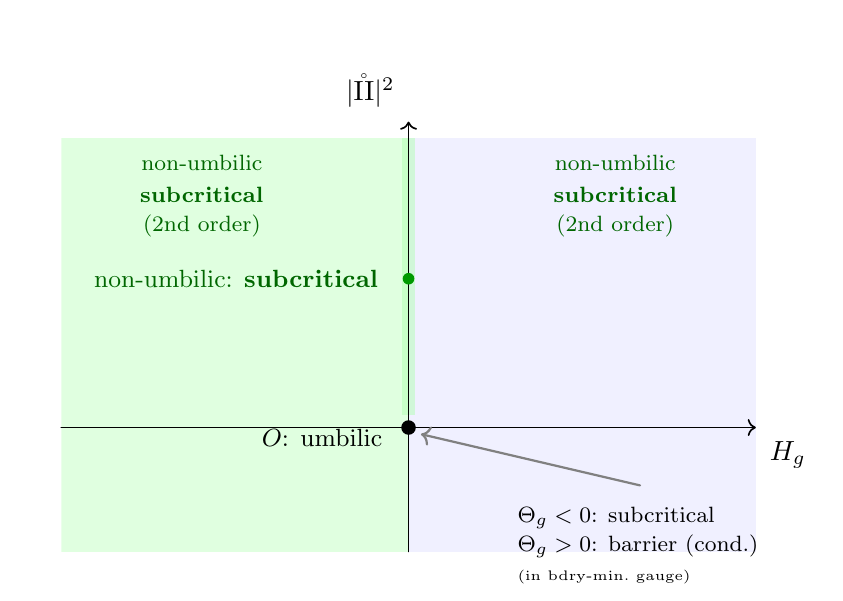
\begin{tikzpicture}[scale=1.05,line cap=round]
  %% bounding box
  \draw[white] (-4.6,-2.2) rectangle (4.6,4.0);

  %% background shading
  \begin{scope}
    \clip (-4.2,-1.5) rectangle (4.2,3.5);
    \fill[green!12] (-4.2,-1.5) rectangle (0,3.5);
    \fill[blue!6] (0,-1.5) rectangle (4.2,3.5);
  \end{scope}

  %% vertical axis highlight strip for non-umbilic subcriticality
  \fill[green!30,opacity=0.5] (-0.08,0.15) rectangle (0.08,3.5);

  %% axes
  \draw[->,semithick] (-4.2,0) -- (4.2,0) node[below right=2pt] {$H_g$};
  \draw[->,semithick] (0,-1.5) -- (0,3.7) node[above left=2pt] {$|\mathring{\mathrm{II}}|^2$};

  %% key points
  \fill (0,0) circle (2.5pt);
  \fill[green!60!black] (0,1.8) circle (2pt);

  %% point labels - non-umbilic label goes LEFT to avoid right-half collision
  \node[anchor=south east,font=\small] at (-0.2,-0.35) {$O$: umbilic};
  \node[anchor=east,font=\small,green!40!black] at (-0.25,1.8)
    {non-umbilic: \textbf{subcritical}};

  %% region labels (well inside each half)
  \node[font=\footnotesize,green!40!black,align=center] at (-2.5,2.8)
    {non-umbilic\\[1pt]\textbf{subcritical}\\(2nd order)};
  \node[font=\footnotesize,green!40!black,align=center] at (2.5,2.8)
    {non-umbilic\\[1pt]\textbf{subcritical}\\(2nd order)};

  %% arrow to origin with Theta_g annotation (lower right)
  \draw[->,thick,gray] (2.8,-0.7) -- (0.15,-0.08);
  \node[font=\footnotesize,anchor=north west,align=left] at (1.2,-0.85)
    {$\Theta_g<0$: subcritical\\
     $\Theta_g>0$: barrier (cond.)\\
     {\tiny(in bdry-min.\ gauge)}};
\end{tikzpicture}

\vspace{6pt}

\noindent\begin{minipage}{0.90\linewidth}
\small
\emph{Reading guide.}  The vertical coordinate records
$|\mathring{\mathrm{II}}|^2$.  Away from the umbilic axis, the reduced
second-order coefficient is negative and gives subcriticality.  At the umbilic
origin the second-order channel vanishes, and the displayed sign of $\Theta_g$
indicates the cubic alternative in a boundary-minimal representative.
\end{minipage}

\caption{Phase diagram for the boundary Escobar problem at the hemisphere threshold,
reflecting the exact second-order cancellation $\kappa_1=\kappa_2=0$.
Since $\kappa_3^{\mathrm{red}}<0$ for all $n\ge5$
(Propositions~\ref{prop:kappa-explicit} and~\ref{prop:dkappa5-lower-bound}),
every non-umbilic zero-mean-curvature boundary point forces strict subcriticality.
The only genuinely degenerate stratum is $\{\mathring{\mathrm{II}}=0\}$
(the origin $O$), where threshold selection is governed by $\Theta_g$
in a fixed boundary-minimal representative:
$\Theta_g<0$ implies subcriticality, while for $n\ge7$ the sign $\Theta_g>0$ gives
threshold compactness (Theorem~\ref{thm:compactness-umbilic}).
No conformal invariance of $\Theta_g$ is asserted.
All entries assume $(M,g)\not\cong_{\mathrm{conf}}(S^n_+,g_{\mathrm{round}})$.}
\label{fig:phase-diagram-escobar}
\end{figure}


\section{Escobar I: Hemisphere coercivity, transfer to \texorpdfstring{$(M,g)$}{(M,g)}, and first-order expansion}
\label{sec:escobar}

\medskip
\noindent\textbf{Standing dimension.} Throughout this section we assume $n\ge 3$.

\medskip
\noindent\emph{Dimension split.}
All first-order statements (in particular the coefficient $\rho_n^{\mathrm{conf}}$ in the
one-bubble expansion and the associated scale-deficit laws) are developed for every $n\ge 3$,
but the analytic mechanisms differ between low and high dimensions.
For $n\ge 4$ we compute $\rho_n^{\mathrm{conf}}$ explicitly from global weighted moments of the
half-space optimizer $U_+$ on $\R^n_+$. In dimension $n=3$ the corresponding weighted moments
diverge logarithmically, and the first-order correction to the Escobar quotient is
$\gamma_3H_g(x)\varepsilon\log(1/\varepsilon)$ (not $\rho_3H_g\varepsilon$);
the conformal cancellation mechanism (Lemma~\ref{lem:rho-positive}) shows
$\gamma_3=0$ as well, so no first-order $H_g$-selection occurs in any dimension.
The second- and third-order coefficients $\mathfrak R_g$ and $\Theta_g$ (renormalized mass
and third-order term) will be used \emph{systematically only for $n\ge 5$ and $n\ge 6$, respectively}
(the borderline cases $n=4$ at second order and $n=5$ at third order require logarithmic renormalization
which we do not pursue). In dimensions $n=3$ and $n=4$
we do not rely on a full renormalized second/third-order Escobar expansion; the results in
Sections~\ref{sec:escobar-second}-\ref{sec:reduced} that require $\mathfrak R_g$ or
$\Theta_g$ are therefore stated and used there under the standing conventions $n\ge 5$ and $n\ge6$.


\noindent\textbf{Standing assumption on the Escobar functional.}
\textbf{(Y$^+_{\partial}$)} Strict coercivity.

By Green's identity for the canonical conformal pair \eqref{eq:canonical-pair}, for every
$u\in C^\infty(M)$ one has
\[
\int_M uL_g^{\circ}udV_g+\int_{\partial M} uB_g^{\circ}ud\sigma_g
= \int_M\Big(|\nabla u|_g^2+\frac{n-2}{4(n-1)}\Scal_gu^2\Big)dV_g
 + \frac{n-2}{2}\int_{\partial M}H_gu^2d\sigma_g.
\]
We \emph{define} the covariant Escobar graph form on $H^1(M)$ by the right-hand side:
\begin{equation}\label{eq:Esc-energy-weak}
\mathcal N^\circ(u)
:=\int_M\Big(|\nabla u|_g^2+\frac{n-2}{4(n-1)}\Scal_gu^2\Big)dV_g
 + \frac{n-2}{2}\int_{\partial M}H_gu^2d\sigma_g,
\qquad u\in H^1(M).
\end{equation}
The associated symmetric bilinear form is defined by polarization:
\begin{equation}\label{eq:Esc-energy-bilinear}
\begin{aligned}
\mathcal N_g^\circ(u,v)
&:=
\int_M
\left(
\langle\nabla u,\nabla v\rangle_g
+
\frac{n-2}{4(n-1)}\Scal_g\,uv
\right)dV_g                                      \\
&\qquad
+
\frac{n-2}{2}
\int_{\partial M}H_g\,uv\,d\sigma_g .
\end{aligned}
\end{equation}
Thus
\[
\mathcal N^\circ(u)=\mathcal N_g^\circ(u,u).
\]
When it is useful to emphasize the metric, we write
$\mathcal N_g^\circ(u):=\mathcal N_g^\circ(u,u)$; otherwise
$\mathcal N^\circ$ suppresses the subscript.
Our standing hypothesis is the strict coercivity
\begin{equation}\label{eq:Yplus}
\mathcal N^\circ(u)\ \ge\ c_Y\|u\|_{H^1(M)}^2\qquad\forall u\in H^1(M).
\end{equation}
Under \textup{(BG$^{2+}$)} the coefficients $\Scal_g,H_g$ are bounded and the global trace
$H^1(M)\to L^2(\partial M)$ is continuous (Lemma~\ref{lem:global-trace}), hence there is $C<\infty$ with
\begin{equation}\label{eq:Esc-energy-continuity}
\mathcal N^\circ(u)\ \le\ C\|u\|_{H^1(M)}^2\qquad\forall u\in H^1(M).
\end{equation}
Consequently $\|u\|_{E,g}:=\sqrt{\mathcal N^\circ(u)}$ is equivalent to $\|u\|_{H^1(M)}$.

\medskip
\noindent\emph{Escobar sharp constant.}
Define
\begin{equation}\label{eq:Esc-sharp-constant}
C^*_{\mathrm{Esc}}(M,g):=\inf_{u\in H^1(M)\setminus\{0\}}
\frac{\mathcal N^\circ(u)}{\|u\|_{L^{2^*_\partial}(\partial M)}^2},
\qquad 2^*_\partial=\frac{2(n-1)}{n-2}.
\end{equation}
By \eqref{eq:Yplus} and the global trace inequality
$\|u\|_{L^{2^*_\partial}(\partial M)}\le C_{\mathrm{tr}}\|u\|_{H^1(M)}$ (Lemma~\ref{lem:global-trace}),
\begin{equation}\label{eq:Esc-strict-positive}
C^*_{\mathrm{Esc}}(M,g)\ \ge\ c_YC_{\mathrm{tr}}^{-2}\ >\ 0.
\end{equation}

    Such a condition~\eqref{eq:Yplus} seems standard in the Yamabe/Escobar community (see for example \cite{EscobarAnnals92,EscobarJDG92, Marques2005,HanLi1999}) for guaranteeing the well-posedness needed for subsequent stability and blow-up analysis, and also in other areas of conformal geometry/minimal surfaces (for example, positivity of the first Steklov eigenvalue ($\sigma_1>0$) in the work of Fraser--Schoen~\cite{FraserSchoen2011} on minimal surfaces).


\noindent\textbf{Standing assumption on the manifold.}
We work on a smooth Riemannian manifold with smooth boundary $(M^n,g)$ of \emph{bounded geometry up to order $k$}, denoted \textup{(BG$^{k+}$)}. This means there exist constants $r_0>0$ and families of numbers $\{C_j\}_{0\le j\le k-2}$, $\{\widetilde C_j\}_{0\le j\le k-1}$ such that:
\begin{enumerate}[label=(\roman*),leftmargin=1.25em]
\item (\emph{Uniform radii of charts}) The interior injectivity radius satisfies $\operatorname{inj}(M,g)\ge r_0$, and the normal exponential map induces a Fermi collar
\[
\exp^\perp:\ \{(x,t)\in T^\perp\partial M:\ 0\le t<r_0\}\longrightarrow \{p\in M:\ 0\le \dist_g(p,\partial M)<r_0\}
\]
 which is a diffeomorphism onto its image. Equivalently, one has geodesic normal charts on $B_{r_0}(x)\subset M^\circ$ and Fermi charts on a boundary collar of width $r_0$.
\item (\emph{Uniform curvature bounds}) The Riemann curvature tensor and its covariant derivatives up to order $k-2$ are uniformly bounded:
\[
\sup_{M}\bigl|\nabla^j \operatorname{Rm}_g\bigr|\ \le C_j,\qquad 0\le j\le k-2.
\]
\item (\emph{Uniform second-fundamental form bounds}) The second fundamental form $\II$ of $\partial M$ and its \emph{tangential} covariant derivatives up to order $k-1$ are uniformly bounded:
\[
\sup_{\partial M}\bigl|\nabla^{j}_{{}^\top}\II\bigr|\ \le \widetilde C_j,\qquad 0\le j\le k-1,
\]
 where $\nabla_{{}^\top}$ is the Levi-Civita connection of the induced metric on $\partial M$.
\end{enumerate}
\begin{lemma}[Global trace under a uniform collar]\label{lem:global-trace}
Assume \textup{(BG$^{2+}$)}. Then there exists $C_{\mathrm{tr}}<\infty$, depending only on the \textup{(BG$^{2+}$)} data, such that for all $u\in H^1(M)$,
\[
\|u\|_{L^2(\partial M)} + \|u\|_{L^{2^*_\partial}(\partial M)} \ \le\ C_{\mathrm{tr}}\|u\|_{H^1(M)}.
\]
\end{lemma}

\begin{proof}[Proof (standard)]
Let $\mathrm{Tr}:H^1(M)\to H^{1/2}(\partial M)$ be the trace operator. Under \textup{(BG$^{2+}$)} (uniform collar charts and
uniform $C^2$ control of the metric), the usual localization-to-Fermi-charts argument and the Euclidean half-space trace
estimate yield a uniform constant $C$ such that
\[
\|\mathrm{Tr}u\|_{H^{1/2}(\partial M)} \le C\|u\|_{H^1(M)}\qquad\forall u\in H^1(M).
\]
Since $\dim(\partial M)=n-1$, the Sobolev embedding $H^{1/2}(\partial M)\hookrightarrow L^{2^*_\partial}(\partial M)$ gives
\[
\|u\|_{L^{2^*_\partial}(\partial M)} \le C\|u\|_{H^{1/2}(\partial M)}.
\]
Also $H^{1/2}(\partial M)\hookrightarrow L^2(\partial M)$, hence $\|u\|_{L^2(\partial M)}\le C\|u\|_{H^{1/2}(\partial M)}$.
Combining these inequalities yields the claim with $C_{\mathrm{tr}}=C^2$.
\end{proof}

Under \textup{(BG$^{k+}$)} the metric coefficients $g_{ab}$ in any such normal/Fermi chart have all partial derivatives up to order $k$ uniformly bounded (uniform $C^k$ control of metric jets).
\begin{lemma}[Uniform $C^k$ Fermi jets from \textup{(BG$^{k+}$)}]\label{lem:fermi-jets}
Under \textup{(BG$^{k+}$)}, the metric coefficients in any Fermi chart on the collar $\{0\le t<r_0\}$ possess uniform $C^k$ bounds (in tangential variables and in the normal variable $t$), with constants depending only on the \textup{(BG$^{k+}$)} data. In particular, all mixed normal/tangential derivatives of total order $\le k$ are uniformly bounded.
\end{lemma}

\begin{proof}[Proof sketch]
Use Gauss-Codazzi and the Riccati ODE $\partial_t \II = -\II^2 + \mathrm{Rm}(\nu,\cdot,\nu,\cdot)$ to control normal derivatives from curvature bounds in (ii), while tangential derivatives are controlled by (iii). A standard bootstrap yields the stated $C^k$ bounds.
\end{proof}

\medskip
\noindent\emph{Order bookkeeping.} The distinction between \textup{(BG$^{k+}$)} and \textup{(BG$^{(k+1)+}$)} is one of available derivatives: \textup{(BG$^{(k+1)+}$)} adds one more bounded curvature derivative (up to order $k-1$) and one more bounded tangential derivative of $\II$ (up to order $k$), hence promotes uniform $C^k$ to uniform $C^{k+1}$ control of the metric jets in local coordinates. In particular, to produce an $O(\varepsilon^m)$ coefficient in the small-radius Fermi/normal expansion with a uniform $O(\varepsilon^{m+1})$ remainder, one assumes \textup{(BG$^{(m+1)+}$)}.

\medskip
\noindent\emph{Thresholds used in this paper.}
\begin{itemize}[leftmargin=1.25em]
\item \textup{(BG$^{2+}$)} (uniform $C^2$ control of $g$ and a fixed Fermi collar) suffices for all
\emph{first-order} energy expansions (the $O(\varepsilon)$ term with $O(\varepsilon^2)$ remainder)
in every dimension $n\ge 3$. For $n\ge 5$, the second-order coefficient $\mathfrak R_g$ is developed in \S\ref{sec:escobar-second};
to obtain an $O(\varepsilon^2)$ coefficient with a uniform $O(\varepsilon^3)$ remainder we work under
\textup{(BG$^{3+}$)} (and for the third-order refinement under \textup{(BG$^{4+}$)}).
\item \textup{(BG$^{4+}$)} (uniform $C^4$ control) is needed, for $n\ge 6$, for the full higher-order
Escobar expansion (the $O(\varepsilon^2)$ coefficient $\mathfrak R_g$ together with the
$O(\varepsilon^3)$ term $\Theta_g$) with a uniform $O(\varepsilon^4)$ remainder (available for $n\ge7$), which is used in the
finer observability and multi-bubble selection arguments.
\end{itemize}


\iffalse
\paragraph{Canonical conformal pair and Escobar functional.}
\begin{equation}\label{eq:conformal-pair}
L^{\circ}_g \coloneqq -\Delta_g + \frac{n-2}{4(n-1)}R_g,
\qquad
B^{\circ}_g \coloneqq -\partial_{\nu} + \frac{n-2}{2}H_g.
\end{equation}
For $q= 2^\sharp := \frac{2(n-1)}{n-2}$ for $n\geq 3$,
\begin{equation}\label{eq:Esc-functional-canonical}
\mathcal E_g[u]
:= \frac{\displaystyle \int_M uL_g^{\circ}udV_g +\int_{\partial M} uB_g^{\circ}ud\sigma_g}
{\Big(\displaystyle\int_{\partial M}|u|^{q}d\sigma_g\Big)^{2/q}},
\qquad u\in H^1(M)\setminus\{0\}.
\end{equation}
Write $S_\ast:=C_{\Esc}^*(S^n_+,g_{\mathrm{round}})$ and
$\Def^{\Esc}_g(u):=\mathcal E_g[u]-C_{\Esc}^*(g)$.
\fi


\subsection{Basic notation and conventions for \S\ref{sec:escobar}}
\label{subsec:escobar-notation}

\paragraph{\emph{Geometry, charts, and indices.}}
For $x\in\partial M$, $\Phi_x:\varepsilon B_{2R}^+\to M$ denotes a Fermi chart centered at $x$ with respect to the \emph{inner} unit normal $\nu$.  We fix $R>0$ and only consider $0<\varepsilon<\varepsilon_0:=\frac{r_0}{4R}$, so that $\varepsilon B_{2R}^+\subset\{0\le t<r_0\}$ and $\Phi_x(\varepsilon B_{2R}^+)$ lies inside the fixed Fermi collar from \textup{(BG$^{k+}$)}.
Throughout, the inner normal is used, i.e. $t\ge 0$.
We write
\[
y=(y',y_n)\in\R^{n-1}\times[0,\infty),\qquad B_{R}^+:=B_R\cap\R^n_+,
\]
and use Einstein summation for tangential indices $a,b\in\{1,\dots,n-1\}$. The induced boundary metric is $\bar g=g|_{T\partial M}$, and we raise/lower tangential indices with $\bar g$ and its inverse $\bar g^{-1}$.
\medskip
\paragraph{\emph{Second fundamental form and mean curvature.}}
$\mathrm{II}=\{\mathrm{II}_{ab}\}$ is the second fundamental form of $\partial M$ in $(M,g)$, with $\mathrm{II}^{ab}:=\bar g^{ac}\bar g^{bd}\mathrm{II}_{cd}$.
We write
\[
K_g:=\mathrm{tr}_{\bar g}\mathrm{II}=\bar g^{ab}\mathrm{II}_{ab},\qquad
H_g:=\frac{K_g}{n-1}
\]
for the trace and averaged mean curvatures, respectively,
taken with respect to the \emph{inner} normal.
With this sign, strictly convex Euclidean domains (e.g.\ the Euclidean ball) have $K_g,H_g>0$ (Remark~\ref{rem:sign-sanity}). We write $\mathring{\mathrm{II}}$ for the traceless part: $\mathrm{II}^{ab}=H_g\bar g^{ab}+\mathring{\mathrm{II}}^{ab}$.
In the conformal Escobar operator the averaged curvature $H_g$ appears; in Fermi-coordinate geometry the trace $K_g$ appears.
\medskip
\paragraph{\emph{Quadratic form $\mathcal Q_g$ and the canonical pair.}}
We set
\[
a_n:=\frac{4(n-1)}{n-2}.
\]
For the \emph{canonical} Escobar pair we fix
\begin{equation}\label{eq:canonical-pair}
L_g^{\circ}:=-\Delta_g+\frac{n-2}{4(n-1)}\Scal_g,\qquad
B_g^{\circ}:=-\partial_\nu+\frac{n-2}{2}H_g.
\end{equation}
The associated weak energy on $H^1(M)$ is (cf.\ \eqref{eq:Esc-energy-weak} upstream with $\alpha_n=1$, $\beta_n=\tfrac{n-2}{2}$)
\[
\mathcal N^\circ(u):=\int_M\Big(|\nabla u|_g^2+\frac{n-2}{4(n-1)}\Scal_gu^2\Big)dV_g
+\int_{\partial M}\frac{n-2}{2}H_gu^2d\sigma_g.
\]
We then define
\[
\mathcal Q_g(u):=a_n\int_M|\nabla u|_g^2dV_g+\int_M \Scal_gu^2dV_g
+2\int_{\partial M}K_gu^2d\sigma_g.
\]
For $u\in C^\infty(M)$, Green's identity gives
\begin{equation}\label{eq:bridge-firstorder}
\int_M uL_g^{\circ}udV_g+\int_{\partial M}uB_g^{\circ}ud\sigma_g
=\mathcal N^\circ(u),\qquad
\mathcal Q_g(u)=a_n\mathcal N^\circ(u),
\end{equation}
and by density these identities hold for all $u\in H^1(M)$ interpreting the left-hand side via the right-hand side.
\medskip
\paragraph{\emph{Escobar quotient and deficit.}}
The Escobar quotient is
\[
\mathcal J_g[u]:=\frac{\mathcal N^\circ(u)}{\|u(\cdot)\|_{L^{2^*_\partial}(\partial M)}^2},\qquad
2^*_\partial=\frac{2(n-1)}{n-2},
\]
and the sharp constant $C^*_{\Esc}(M,g):=\inf_{u\ne 0}\mathcal J_g[u]$ is strictly positive by \textup{(Y$^+_{\partial}$)} and the global trace. The (nonnegative) covariant Escobar deficit is
\[
\Def^{\Esc}_g(u):=\mathcal J_g[u]-C^*_{\Esc}(M,g)\ \ge 0.
\]

\paragraph{\emph{Half-space notation and tangential gradient.}}
On $\R^n_+$ we write $\nabla_{\tan}w:=(\partial_{y_a}w)_{a=1}^{n-1}$ and $dy$ for Lebesgue measure; $d\sigma$ denotes the flat boundary measure on $\{y_n=0\}$.
\medskip
\paragraph{\emph{Fermi pushforward at the critical trace scaling.}}
For $w$ on $\R^n_+$ (compactly supported in $B_{2R}^+$, or as a limit of such truncations),
\[
(\mathcal T_{x,\varepsilon}w)(z)
:=\varepsilon^{-\frac{n-2}{2}}w\Big(\frac{\Phi_x^{-1}(z)}{\varepsilon}\Big)\quad
\text{for }z\in \Phi_x(\varepsilon B_{2R}^+),\qquad 0\ \text{outside}.
\]
When $w$ is not compactly supported we insert a fixed smooth cutoff $\chi_R$ equal to $1$ on $B_R^+$ and define $\mathcal T_{x,\varepsilon}(\chi_R w)$; all first-order (resp.\ second-order) formulas are independent of the choice of $\chi_R$ under \textup{(BG$^{2+}$)} (resp.\ \textup{(BG$^{3+}$)} or \textup{(BG$^{4+}$)} depending on the remainder chosen earlier). We keep the shorthand $v_{x,\varepsilon}:=\mathcal T_{x,\varepsilon}(\chi_R w)$, suppressing $R$.
\medskip
\paragraph{\emph{Model profiles and cutoffs.}}
Fix a half-space optimizer $U_+$ (cf.\ \cite[Eq.~(2)]{Escobar1988}) for the \emph{covariant} Escobar problem on $\R^n_+$. Fix once and for all a representative $U_+$ that is centered at the origin and tangentially radial, and normalize it by
\[
\|\nabla U_+\|_{L^2(\R^n_+)}=1.
\]
Equivalently (since $U_+$ is an optimizer and $S_\ast$ is the sharp constant on the model),
\[
\|U_+(\cdot,0)\|_{L^{2^*_\partial}(\R^{n-1})}^{2}
=\frac{1}{S_\ast}.
\]
We also use the boundary-mass-one representative
\begin{equation}\label{eq:mass-one-Uplus}
U_\ast:=S_\ast^{1/2}U_+.
\end{equation}
Then $\|U_\ast(\cdot,0)\|_{L^{2^*_\partial}}^{2^*_\partial}=1$,
$\|\nabla U_\ast\|_{L^2(\R^n_+)}^2=S_\ast$, and $U_\ast$ solves
$-\Delta U_\ast=0$ in $\R^n_+$,
$-\partial_{y_n}U_\ast=S_\ast U_\ast^{2^*_\partial-1}$ on $\partial\R^n_+$.
All model constants (e.g.\ $\mathfrak g^{(1)}$, $\Theta$) are defined with respect to this fixed, normalized $U_+$.
Similarly, fix a radially symmetric optimizer $U_{\mathrm{int}}$ for the interior Yamabe problem on $\R^n$, normalized by $\|\nabla U_{\mathrm{int}}\|_{L^2(\R^n)}=1$.
Fix a smooth cutoff $\chi\in C_c^\infty(\R^n)$ such that $0\le\chi\le 1$, $\chi(y)=1$ for $|y|\le 1$, and $\chi(y)=0$ for $|y|\ge 2$. For $R\ge 1$, set $\chi_R(y):=\chi(y/R)$.

\begin{definition}[Bubbles and Manifolds]\label{def:bubbles}
Let $(M,g)$ satisfy \textup{(BG$^{2+}$)} with injectivity radius $r_0$.
\begin{enumerate}[label=\textbf{(\roman*)}, leftmargin=1.5em]
    \item \textbf{Boundary bubbles.} For $x\in\partial M$ and $\varepsilon>0$ small, the boundary bubble is defined via the Fermi pushforward $\mathcal T_{x,\varepsilon}$ (from \S\ref{subsec:escobar-notation}):
    \[
    U_{+,x,\varepsilon} \ :=\ \mathcal T_{x,\varepsilon}(\chi_{R(\varepsilon)} U_+),
    \]
    where $R(\varepsilon):=\varepsilon^{-3/4}$ (so that $\varepsilon R(\varepsilon)=\varepsilon^{1/4}\to0$ and the Fermi chart support stays inside the collar for $\varepsilon$ small).
    (Explicitly: $U_{+,x,\varepsilon}(z) = \varepsilon^{-\frac{n-2}{2}}(\chi_{R(\varepsilon)} U_+)\big(\Phi_x^{-1}(z)/\varepsilon\big)$ inside the Fermi chart).

    \item \textbf{Interior bubbles.} For $x\in M^\circ$ and $\varepsilon>0$ small (assuming $\dist_g(x,\partial M) > 2R(\varepsilon)\varepsilon$), let $\Psi_x$ be a geodesic normal chart at $x$. The interior bubble is
    \[
    U^{\mathrm{int}}_{x,\varepsilon}(z) \ :=\ \varepsilon^{-\frac{n-2}{2}}(\chi_{R(\varepsilon)} U_{\mathrm{int}})\left(\frac{\Psi_x^{-1}(z)}{\varepsilon}\right).
    \]

    \item \textbf{Bubble manifolds.} We define the submanifolds of $H^1(M)$ by:
    \[
    \mathcal B_\partial := \{ U_{+,x,\varepsilon} : x\in\partial M, \varepsilon>0 \},
    \qquad
    \mathcal B_{\mathrm{int}} := \{ U^{\mathrm{int}}_{x,\varepsilon} : x\in M^\circ, \varepsilon>0 \}.
    \]
\end{enumerate}
\end{definition}

\begin{remark}[Cutoff conventions]\label{rem:bubble-cutoff}
The diagonal choice $R(\varepsilon)=\varepsilon^{-3/4}$ is used throughout. It ensures:
\begin{enumerate}[label=(\alph*)]
\item The cutoff residual $\omega(R(\varepsilon))\downarrow0$ as $\varepsilon\downarrow0$, so all
cutoff-independent coefficients ($\rho_n^{\mathrm{conf}}$, $\mathfrak R_g$, etc.) are
realized in the limit. In particular, $\mathcal J_g[U_{+,x,\varepsilon}]\to S_\ast$.
\item For $n\ge5$, the cutoff-variation terms in the modulation
directions $\partial_\varepsilon U_{+,x,\varepsilon}$
and $\partial_x U_{+,x,\varepsilon}$ have
$H^1(M)$-norm $O(\varepsilon^{(3n-14)/8})=o(1)$
(since $(3n-14)/8>0$ when $n\ge5$), so the
modulation IFT (Lemma~\ref{lem:modulation}) applies to this family.
In the blow-up proof of Theorem~\ref{thm:intrinsic-single-gap},
$\chi_{R(\varepsilon_k)}\to1$ locally on every fixed ball, so the
rescaled Hessian converges to the flat Hessian at $U_+$.
\item In Section~\ref{sec:reduced} (multi-bubble theory), the same diagonal choice
ensures exact disjoint supports under macroscopic separation.
\end{enumerate}
For $n=3,4$, the first-order quotient expansion
(Lemma~\ref{lem:esc-scale-law}) is a direct computation
that does not require the modulation/coercivity package.
The quantitative coercivity and threshold theory (which begins at $n\ge5$) is not affected.
\end{remark}


\paragraph{\emph{Modulation directions.}}
For $v^\sharp=U_{+,x,\varepsilon}$, the tangent (neutral) directions are
\[
\partial_\varepsilon U_{+,x,\varepsilon},\qquad \nabla_x U_{+,x,\varepsilon}=\big(\partial_{x^\alpha}U_{+,x,\varepsilon}\big)_{\alpha=1}^{n-1},
\]
and we impose \emph{graph-orthogonality} $\langle u-v^\sharp,\partial_\varepsilon U_{+,x,\varepsilon}\rangle_{E,g}=0$ and
$\langle u-v^\sharp,\partial_{x^\alpha} U_{+,x,\varepsilon}\rangle_{E,g}=0$ in the modulation lemmas.
\medskip
\paragraph{\emph{Cayley transform and spherical optimizer.}}
The Cayley transform $\mathcal C:S^n_+\to\R^n_+$ is the standard conformal diffeomorphism; if $U_+$ is fixed on $\R^n_+$, its Cayley pullback $F_\ast:=\mathcal C^\ast U_+$ lies on the optimizer manifold $\mathcal M_S$ on $(S^n_+,g_{\mathrm{round}})$. We write $E:=T_{F_\ast}\mathcal M_S$ for the tangent space to $\mathcal M_S$ generated by boundary-preserving conformal motions.

\paragraph{\emph{First-order moments on $\R^n_+$.}}\label{par:moments-first}
For the (harmonic) optimizer $U_+$ we set, in dimensions $n\ge4$,
\[
\mathfrak g^{(1)}:=\frac{\int_{\R^n_+} y_n|\nabla U_+|^2dy}{\int_{\R^n_+}|\nabla U_+|^2dy},
\qquad
\mathfrak g^{(1)}_{\tan}:=\frac{\int_{\R^n_+} y_n|\nabla_{\tan}U_+|^2dy}{\int_{\R^n_+}|\nabla U_+|^2dy},
\qquad
\Theta:=\frac{\|U_+(\cdot,0)\|_{L^2(\R^{n-1})}^2}{\|\nabla U_+\|_{L^2(\R^n_+)}^2}.
\]
These quantities are finite for $n\ge4$ and enter the explicit formula for the first-order
coefficient $\rho_n^{\mathrm{conf}}$ in \eqref{eq:rho-conf-correct}, cf.\
Lemmas~\ref{lem:harmonic-y-moments} and~\ref{lem:rho-positive}.

In dimension $n=3$ we do \emph{not} use the individual moments
$\mathfrak g^{(1)},\mathfrak g^{(1)}_{\tan},\Theta$: the corresponding weighted
integrals for the model optimizer diverge logarithmically.  The first-order law is
therefore logarithmic rather than linear.  See Remark~\ref{rem:n3-renorm} for the
cutoff convention and the coefficient $\gamma_3$; the same conformal cancellation mechanism applies
(Lemma~\ref{lem:rho-positive}), so $\gamma_3=0$ and no first-order $H_g$-selection
occurs in dimension $3$ either.

\medskip
\paragraph{\emph{Big-O with chart radius.}}
The symbol $O_R(\varepsilon^2)$ means a bound $\le C(R)\varepsilon^2$ with $C(R)$ independent of the center $x$ (by (BG)) and acting on the appropriate quadratic norm of $w$ (e.g.\ $\|w\|_{H^1(B_{2R}^+)}^2$). We use the same convention for $O_R(\varepsilon)$. Under \textup{(BG$^{2+}$)} the constants $C(R)$ are uniform in $x$ thanks to the uniform $C^2$ bounds of the Fermi jets; for higher-order remainders we use \textup{(BG$^{3+}$)} or \textup{(BG$^{4+}$)} accordingly.
\medskip
\paragraph{\emph{Tangential radiality.}}
A function $w$ on $\R^n_+$ is \emph{tangentially radial} if $w(y',y_n)=W(|y'|,y_n)$; then $|\nabla_{\tan}w|^2=W_r^2$ and the traceless part $\mathring{\mathrm{II}}$ averages out in first-order corrections (cf.\ \eqref{eq:Q-isotropic}).


\subsection{Toolkit in Fermi charts (first order)}
\begin{lemma}[Uniform Fermi atlas and Jacobian control]\label{lem:atlas}
Assume \textup{(BG$^{2+}$)}. Then there exists an atlas of interior normal and boundary Fermi charts with uniform $C^2$ bounds and bilipschitz constants (independent of the center and chart), so that the Jacobians and their first derivatives are uniformly controlled on fixed chart radii. In particular, Euclidean capacity and trace estimates transfer to $(M,g)$ with constants depending only on the \textup{(BG$^{2+}$)} data (cf.\ Lemma~\ref{lem:global-trace}).
\end{lemma}

\begin{lemma}[Near-isometry of the energy with first-order geometric correction]\label{lem:near-iso-energy}
Let $(M^n,g)$ satisfy \textup{(BG$^{2+}$)} near a boundary point $x\in\partial M$.  Fix a Fermi chart $\Phi_x:B_{r_0}^+\to M$ adapted to the \emph{inner} unit normal, and for $0<\varepsilon<\varepsilon_0(R)$ use its restriction to $\varepsilon B_{2R}^+$.
 For $w\in H^1(\R^n_+)$ compactly supported in $B^+_{2R}$ and $u_\varepsilon:=\mathcal T_{x,\varepsilon}w$, we have
\begin{align}
\mathcal Q_g(u_\varepsilon)
&= a_n\int_{\R_+^n} |\nabla w|^2dy
+ a_n\varepsilon\int_{\R_+^n} y_n\Big(2\mathrm{II}^{ab}(x)\partial_{y_a}w\partial_{y_b}w - K_g(x)|\nabla w|^2\Big)dy \nonumber\\
&\quad + 2\varepsilon K_g(x)\|w(\cdot,0)\|_{L^2(\R^{n-1})}^2
+ O_R(\varepsilon^2)\|w\|_{H^1(B^+_{2R})}^2. \label{eq:Q-first-order}
\end{align}
Here $H_g=\frac{1}{n-1}\mathrm{tr}_{\bar g}\mathrm{II}$ is the mean curvature with respect to the inner normal. If, in addition, $w$ is tangentially radial, then the traceless part of $\mathrm{II}$ averages out and
\begin{align}
\mathcal Q_g(u_\varepsilon)
&= a_n\int_{\R_+^n} |\nabla w|^2dy \nonumber\\
&\quad + a_n\varepsilon K_g(x)\left[\frac{2}{n-1}\int_{\R_+^n} y_n|\nabla_{\tan} w|^2dy - \int_{\R_+^n} y_n|\nabla w|^2dy\right] \nonumber\\
&\quad + 2\varepsilon K_g(x)\|w(\cdot,0)\|_{L^2(\R^{n-1})}^2
+ O_R(\varepsilon^2)\|w\|_{H^1(B^+_{2R})}^2.
\label{eq:Q-isotropic}
\end{align}
\end{lemma}

\begin{proof}
Fix $R<\infty$ and $\varepsilon\in(0,\varepsilon_0(R))$. Write $y=(y',y_n)$ in Fermi coordinates at $x\in\partial M$
(boundary geodesic normal, extended by Fermi transport along the inner normal) and set
$u_\varepsilon(z)=\varepsilon^{-(n-2)/2}w(y)$ with $z=\Phi_x(\varepsilon y)$.
By \textup{(BG$^{2+}$)} and standard Fermi theory
(see \cite[\S2]{EscobarJDG92}, \cite[Ch.~2]{Aubin98}):
\begin{align}
g^{ab}(\varepsilon y)\sqrt{|g(\varepsilon y)|}
&=\delta^{ab}+\varepsilon y_n\big(2\mathrm{II}^{ab}(x)-K_g(x)\delta^{ab}\big)+O_R(\varepsilon^2),
\label{eq:F2}\\
g^{nn}(\varepsilon y)\sqrt{|g(\varepsilon y)|}
&=1-\varepsilon K_g(x)y_n+O_R(\varepsilon^2),\qquad g^{an}\sqrt{|g|}=O_R(\varepsilon^2).
\notag
\end{align}
Changing variables and expanding gives
\begin{equation}\label{eq:E2}
\int_M |\nabla u_\varepsilon|_g^2dV_g
=\int_{B^+_{2R}}|\nabla w|^2dy + \varepsilon\int_{B^+_{2R}} y_n\big(2\mathrm{II}^{ab}(x)\partial_{y_a}w\partial_{y_b}w - K_g(x)|\nabla w|^2\big)dy
+O_R(\varepsilon^2)\|w\|_{H^1}^2.
\end{equation}
The scalar-curvature term is $O_R(\varepsilon^2)\|w\|_{H^1}^2$ (since $\Scal_g$ enters at $O(\varepsilon^2)$ after rescaling).
For the boundary mean-curvature term, $H_g(\Phi_x(\varepsilon y',0))=H_g(x)+O(\varepsilon|y'|)$ gives
\begin{equation}\label{eq:E4}
\int_{\partial M} H_gu_\varepsilon^2dS_g
=\varepsilon H_g(x)\|w(\cdot,0)\|_{L^2(\R^{n-1})}^2+O_R(\varepsilon^2)\|w\|_{H^1}^2.
\end{equation}
Assembling gives \eqref{eq:Q-first-order}.
For tangentially radial $w$, isotropy of $\mathbb S^{n-2}$ kills the $\mathring{\mathrm{II}}$-trace
($\int_{\mathbb S^{n-2}}\omega_a\omega_b=\frac{\mathrm{Area}(\mathbb S^{n-2})}{n-1}\delta_{ab}$),
yielding \eqref{eq:Q-isotropic}.
\end{proof}


\begin{lemma}[Boundary trace at critical scaling has no $O(\varepsilon)$ correction]\label{lem:trace-no-linear}
Let $n\ge 3$ and let $w\in H^1(\R^n_+)$ be supported in $B_{2R}^+$ with
$w(\cdot,0)\in L^{2^*_{\partial}}(\R^{n-1})$, where $2^*_{\partial}=\frac{2(n-1)}{n-2}$.
Assume \textup{(BG$^{2+}$)}. Then, for each fixed $R<\infty$ there exists
$\varepsilon_0(R)>0$ such that for all $0<\varepsilon<\varepsilon_0(R)$,
\[
\big\|\big(\mathcal T_{x,\varepsilon}w\big)\big|_{\partial M}\big\|_{L^{2^*_{\partial}}(\partial M)}^{2^*_{\partial}}
\ =\ \big(1+O_R(\varepsilon^2)\big)\|w(\cdot,0)\|_{L^{2^*_{\partial}}(\R^{n-1})}^{2^*_{\partial}}
\]
uniformly in $x\in\partial M$, where $O_R(\varepsilon^2)$ denotes a quantity bounded by
$C(R)\varepsilon^2$ with $C(R)$ depending only on $R$ and the \textup{(BG$^{2+}$)} data.
\end{lemma}

\begin{proof}
Work in a boundary Fermi chart $\Phi_x$ centered at $x\in\partial M$, adapted to the inner
unit normal, and write $z=\Phi_x(\varepsilon y)$ with $y=(y',y_n)$ and $y_n\ge0$.
By definition,
\[
(\mathcal T_{x,\varepsilon}w)(z)=\varepsilon^{-\frac{n-2}{2}}w(y),
\qquad z\in \Phi_x(\varepsilon B^+_{2R}),
\]
and $(\mathcal T_{x,\varepsilon}w)(z)=0$ outside this chart image. On the boundary slice
$\{y_n=0\}$ we choose $y'$ to be geodesic normal coordinates for $\bar g$ at $x$. Then,
by \textup{(BG$^{2+}$)} and the standard boundary normal expansion,
\[
g_{ab}(\varepsilon y',0)=\delta_{ab}+O(\varepsilon^2|y'|^2),\hspace{2mm}
d\sigma_g\big|_{y_n=0}=\sqrt{\det(g_{ab}(\varepsilon y',0))}\varepsilon^{n-1}dy'
=\varepsilon^{n-1}\big(1+O(\varepsilon^2|y'|^2)\big)dy'.
\]
Since $(\mathcal T_{x,\varepsilon}w)|_{\partial M}$ is supported in
$\Phi_x(\varepsilon B_{2R}\cap\{y_n=0\})$, we can write
\begin{align*}
\int_{\partial M} \big|(\mathcal T_{x,\varepsilon}w)(z)\big|^{2^*_{\partial}}d\sigma_g(z)
&= \int_{\R^{n-1}} \varepsilon^{-\frac{(n-2)2^*_{\partial}}{2}}|w(y',0)|^{2^*_{\partial}}
\cdot \varepsilon^{n-1}\big(1+O(\varepsilon^2|y'|^2)\big)dy'\\
&= \int_{\R^{n-1}} |w(y',0)|^{2^*_{\partial}}\big(1+O(\varepsilon^2|y'|^2)\big)dy',
\end{align*}
because $\frac{(n-2)2^*_{\partial}}{2}=n-1$. Since $w(\cdot,0)$ is supported in $B_{2R}$,
we have $|y'|\le2R$ on the support, so $O(\varepsilon^2|y'|^2)=O_R(\varepsilon^2)$, and
\[
\int_{\R^{n-1}} |w(y',0)|^{2^*_{\partial}}O(\varepsilon^2|y'|^2)dy'
= O_R(\varepsilon^2)\|w(\cdot,0)\|_{L^{2^*_{\partial}}(\R^{n-1})}^{2^*_{\partial}}.
\]
This yields the desired estimate. Uniformity in $x$ follows from the uniformity of the Fermi
expansions under \textup{(BG$^{2+}$)}.
\end{proof}

\begin{lemma}[Weighted harmonic moment identities on $\R^n_+$]\label{lem:harmonic-y-moments}
Let $n\ge2$, let $f\in L^2(\R^{n-1})$, and let $U$ be the Poisson extension of $f$ to
$\R^n_+$, so that $U$ is harmonic in $\R^n_+$ and $U(\cdot,0)=f$ in the trace sense. Then
\begin{equation}\label{eq:moment-equalities}
\int_{\R^n_+} y_n|\nabla U|^2dy = \frac12\|f\|_{L^2(\R^{n-1})}^2,\qquad
\int_{\R^n_+} y_n|\nabla_{\tan} U|^2dy = \int_{\R^n_+} y_n|\partial_{y_n} U|^2dy = \frac14\|f\|_{L^2(\R^{n-1})}^2.
\end{equation}
In particular, if in addition $\nabla U\in L^2(\R^n_+)$ so that the dimensionless moments
from \S\ref{par:moments-first} are finite (for example, for the Escobar optimizer $U_+$ when
$n\ge4$), then
\begin{equation}\label{eq:dimensionless-relations}
\mathfrak g^{(1)} = \frac12\Theta,
\qquad
\mathfrak g^{(1)}_{\tan} = \frac14\Theta.
\end{equation}
\end{lemma}

\begin{proof}
Taking the tangential Fourier transform in $y'$ yields
\[
\widehat{U}(k,y_n)=\hat f(k)e^{-|k|y_n},\qquad k\in\R^{n-1},\ y_n>0,
\]
for the Poisson extension. In Fourier variables,
\[
|\nabla_{\tan}U|^2 \longleftrightarrow |k|^2|\hat f(k)|^2 e^{-2|k|y_n},\qquad
|\partial_{y_n}U|^2 \longleftrightarrow |k|^2|\hat f(k)|^2 e^{-2|k|y_n}.
\]
For $k\neq0$,
\[
\int_0^\infty y_n |k|^2 e^{-2|k|y_n}dy_n
= |k|^2\int_0^\infty y_n e^{-2|k|y_n}dy_n
= \frac{1}{4},
\]
while for $k=0$ the integrand is identically zero, so the inner integral vanishes.
Define
\[
J(k):=\int_0^\infty y_n |k|^2|\hat f(k)|^2 e^{-2|k|y_n}dy_n.
\]
Then $J(k)=\tfrac14|\hat f(k)|^2$ for all $k\neq0$, and $J(0)=0$, so
\[
0\le J(k)\le \tfrac14|\hat f(k)|^2\quad\text{for all }k\in\R^{n-1}.
\]
Using Tonelli and Plancherel,
\begin{align*}
\int_{\R^n_+} y_n|\nabla_{\tan}U|^2dy
&= \int_0^\infty y_n\int_{\R^{n-1}} |k|^2|\hat f(k)|^2 e^{-2|k|y_n}dkdy_n\\
&= \int_{\R^{n-1}} J(k)dk
= \frac14\int_{\R^{n-1}}|\hat f(k)|^2dk
= \frac14\|f\|_{L^2(\R^{n-1})}^2,
\end{align*}
where the last equality holds because the set $\{k=0\}$ has Lebesgue measure zero.
The same computation with $|\partial_{y_n}U|^2$ in place of $|\nabla_{\tan}U|^2$ gives
\[
\int_{\R^n_+} y_n|\partial_{y_n}U|^2dy
= \frac14\|f\|_{L^2(\R^{n-1})}^2.
\]
Adding the two equalities yields
\[
\int_{\R^n_+} y_n|\nabla U|^2dy
= \frac12\|f\|_{L^2(\R^{n-1})}^2.
\]
This proves \eqref{eq:moment-equalities}. The relations \eqref{eq:dimensionless-relations}
follow immediately by dividing by $\|\nabla U\|_{L^2(\R^n_+)}^2$ whenever the dimensionless
quantities are defined.
\end{proof}

\begin{remark}\label{rem:n3-renorm}
In dimension $n=3$ the Escobar optimizer $U_+$ on $\R^3_+$ satisfies
$U_+(y',0)\sim |y'|^{-1}$ as $|y'|\to\infty$, so its $L^2$ trace diverges
logarithmically. Consequently,
\[
\int_{\R^3_+} y_3|\nabla U_+|^2dy,\qquad
\int_{\R^3_+} y_3|\nabla_{\tan} U_+|^2dy
\]
are infinite, and the ratios $\mathfrak g^{(1)}$, $\mathfrak g^{(1)}_{\tan}$ and $\Theta$
(as defined in \S\ref{par:moments-first}) are not meaningful in $n=3$.

Whenever we need harmonic moment identities in $n=3$, we apply
Lemma~\ref{lem:harmonic-y-moments} only to harmonic functions with finite $L^2$ trace
(for instance, harmonic extensions of truncated boundary data), and we use the resulting
identities at the level of intermediate estimates. For the model optimizer $U_+$ itself,
the first-order correction to the Escobar quotient on $(M,g)$ involves a
\emph{logarithmic} term in $n=3$. However, the conformal cancellation mechanism
(Lemma~\ref{lem:rho-positive}) shows that both the boundary and bulk logarithmic
contributions cancel exactly:
\[
\mathcal J_g[v_{x,\varepsilon}]
= S_\ast+ O(\varepsilon),
\]
i.e., the coefficient $\gamma_3$ of $H_g(x)\varepsilon\log(1/\varepsilon)$ vanishes.
No first-order $H_g$-selection occurs in dimension $3$.
\end{remark}

\begin{lemma}[Canonical numerator equals the $a_n$-scaled quadratic form]\label{lem:bridge-firstorder}
Let $n\ge 3$ and set $a_n=\frac{4(n-1)}{n-2}$. Define
\[
\mathcal Q_g(u):=a_n\int_M |\nabla u|_g^2dV_g
+ \int_M \Scal_gu^2dV_g
+ 2\int_{\partial M} K_gu^2d\sigma_g.
\]
Then, for $u\in C^\infty(M)$,
\[
\int_M u L_g^{\circ}udV_g+\int_{\partial M}u B_g^{\circ}ud\sigma_g
=\mathcal N^\circ(u),\qquad
\mathcal Q_g(u)=a_n\mathcal N^\circ(u).
\]
By density, both identities extend to all $u\in H^1(M)$, interpreting the left-hand side
via the right-hand side (weak Green identity).
\end{lemma}

\begin{proof}
Integration by parts (with $\nu$ the \emph{inward} unit normal): $\int_M u(-\Delta_g u)dV_g=\int_M|\nabla u|^2_gdV_g+\int_{\partial M}u\partial_\nu ud\sigma_g$.
Substituting into $\int_M uL_g^\circ udV_g+\int_{\partial M}uB_g^\circ ud\sigma_g$ and collecting terms gives $\mathcal N^\circ(u)$; the scaling $\mathcal Q_g=a_n\mathcal N^\circ$ follows from the definitions.
\end{proof}
Combining Lemmas~\ref{lem:near-iso-energy}, \ref{lem:trace-no-linear},
and~\ref{lem:bridge-firstorder} with a \emph{tangentially radial} profile
$w\in H^1(\R^n_+)$ supported in $B_{2R}^+$ (and $w(\cdot,0)\not\equiv 0$) yields,
for $u_\varepsilon:=\mathcal T_{x,\varepsilon}w$, a first-order expansion of the Escobar
quotient of the form
\[
\mathcal J_g[u_\varepsilon]
= \mathcal J_{\mathrm{flat}}[w]
+ \varepsilon H_g(x)\Lambda[w]
+ O_R(\varepsilon^2),
\]
where $\mathcal J_{\mathrm{flat}}$ is the Escobar quotient on the half-space and
$\Lambda[w]$ is a scalar depending only on $w$ and $n$. The traceless part of $\II$ does
not contribute at first order precisely because $w$ is tangentially radial
(cf.\ \eqref{eq:Q-isotropic}), so the linear term is proportional to $H_g(x)$.

In particular, taking $w=\chi_R U_+$ with $\chi_R$ a fixed smooth \emph{tangentially radial} cutoff
supported in $B_{2R}^+$ and equal to $1$ on $B_R^+$ (so that $\chi_R U_+$ remains tangentially radial), we obtain
\[
\mathcal J_g[u_{\varepsilon,R}]
= \mathcal J_{\mathrm{flat}}[\chi_R U_+]
+ \varepsilon H_g(x)\Lambda[\chi_R U_+]
+ O_R(\varepsilon^2),
\qquad
u_{\varepsilon,R}:=\mathcal T_{x,\varepsilon}(\chi_R U_+).
\]
Since $\|\nabla(\chi_R U_+)-\nabla U_+\|_{L^2(\R^n_+)}\to0$ and $\chi_R U_+(\cdot,0)\to U_+(\cdot,0)$ in
$L^{2^*_\partial}(\R^{n-1})$ as $R\to\infty$,
we have $\mathcal J_{\mathrm{flat}}[\chi_R U_+]\to S_\ast$, and, when $n\ge4$, all the
weighted moments entering the explicit expression of $\Lambda[\chi_R U_+]$ converge to the
corresponding moments of $U_+$ itself by dominated convergence, using the finiteness of
these moments for $U_+$ (see Lemma~\ref{lem:harmonic-y-moments}). In particular, the limit
\[
\Lambda[U_+]:=\lim_{R\to\infty}\Lambda[\chi_R U_+]
\]
exists and depends only on $n$ and on the model optimizer $U_+$.

Writing $v_{x,\varepsilon}:=\mathcal T_{x,\varepsilon}U_+$ for the boundary bubble generated by $U_+$
(implemented via the cutoff convention in \S\ref{subsec:escobar-notation}), it follows that the coefficient of
$\varepsilon H_g(x)$ in the first-order expansion of $\mathcal J_g[v_{x,\varepsilon}]$
at $\varepsilon=0$ is
\[
\rho_n^{\mathrm{conf}}:=S_\ast^{-1}\Lambda[U_+],
\]
so that, for $n\ge4$,
\[
\mathcal J_g[v_{x,\varepsilon}]
= S_\ast\Big(1+\rho_n^{\mathrm{conf}}H_g(x)\varepsilon\Big)
+ o(\varepsilon)\quad\text{as }\varepsilon\downarrow0.
\]

For dimensions $n\ge4$, the first-order coefficient admits the explicit moment formula
\begin{equation}\label{eq:rho-conf-correct}
\rho_n^{\mathrm{conf}}
=\Big(2\mathfrak g^{(1)}_{\tan}-(n-1)\mathfrak g^{(1)}\Big)
+ \tfrac{n-2}{2}\Theta,
\qquad n\ge4,
\end{equation}
where $\mathfrak g^{(1)}$, $\mathfrak g^{(1)}_{\tan}$ and $\Theta$ are as in
\S\ref{par:moments-first}. The first bracket is the bulk gradient contribution
(inverse-metric correction minus Jacobian), and the second term is the boundary
Robin contribution from the conformal Escobar operator.
If, in addition, $U_+$ is harmonic with
$U_+(\cdot,0)\in L^2(\R^{n-1})$ (which holds for the Escobar optimizer when $n\ge4$),
Lemma~\ref{lem:rho-positive} yields
\[
\rho_n^{\mathrm{conf}}
=\left(\tfrac12-(n-1)\tfrac12+\tfrac{n-2}{2}\right)\Theta
=0,\qquad n\ge4.
\]
\smallskip
\noindent\emph{Dimensional note ($n=3$).}
The weighted $L^2$ moments used in \eqref{eq:rho-conf-correct} are not finite
in dimension $3$.  The corresponding logarithmic cancellation is recorded in
Remark~\ref{rem:n3-renorm} and in Lemma~\ref{lem:rho-positive}\textup{(b)}.

\begin{remark}[Sign convention]\label{rem:sign-sanity}
We orient $\nu$ as the \emph{inner} unit normal, so the second fundamental form $\II$ and
mean curvature $H_g=\frac{1}{n-1}\mathrm{tr}_{\bar g}\II$ are computed with respect to the inward
pointing normal. In particular, for the Euclidean unit ball equipped with this convention,
boundary Fermi coordinates give $g_{ab}(t)=(1-t)^2\bar g_{ab}(0)$, so comparison with the
general expansion $g_{ab}(t)=\bar g_{ab}(0)-2t\II_{ab}+O(t^2)$ yields
\[
\II_{ab}=\bar g_{ab}(0),\qquad H_g=1>0,
\]
and strictly convex Euclidean domains have \emph{positive} boundary mean curvature in our
convention.

In the first-order correction to the quadratic form (cf.\ \eqref{eq:Q-isotropic}), the
gradient part contributes
\[
\varepsilon\int_{\R^n_+} y_n\Big(2\mathrm{II}^{ab}\partial_{y_a} w\partial_{y_b} w
- K_g|\nabla w|^2\Big)dy,
\]
where $K_g=\mathrm{tr}_{\bar g}\mathrm{II}$ comes from the Jacobian
determinant of the Fermi metric.
For tangentially radial $w$, the isotropic part of the inverse-metric correction
gives $2H_g|\nabla_{\mathrm{tan}}w|^2$ (using $\mathrm{II}^{ab}=H_g\bar g^{ab}+\mathring{\mathrm{II}}^{ab}$),
and the gradient bracket reduces to
\[
H_g\left(2\int_{\R^n_+} y_n|\nabla_{\tan}w|^2dy
- (n-1)\int_{\R^n_+} y_n|\nabla w|^2dy\right).
\]
The boundary term in $\mathcal Q_g$ contributes
\[
2K_g\varepsilon\|w(\cdot,0)\|_{L^2(\R^{n-1})}^2.
\]
Under the conformal Escobar operator, the bulk gradient correction
$a_nH_g\varepsilon[2\mathfrak g_{\tan}^{(1)}-(n-1)\mathfrak g^{(1)}]
=-a_n\frac{n-2}{2}\Theta H_g\varepsilon$
is exactly cancelled by the boundary contribution
$2(n-1)\Theta H_g\varepsilon = a_n\frac{n-2}{2}\Theta H_g\varepsilon$;
the resulting first-order coefficient vanishes identically
(see Lemma~\ref{lem:Esc-first-order}).
\end{remark}


\subsection{Model coercivity on the hemisphere and transfer}


\paragraph{Constraint slice on the hemisphere.}
Let $F_\ast$ denote the Cayley pullback to $(S^n_+,g_{\mathrm{round}})$ of a fixed half-space optimizer $U_+$ for the covariant Escobar problem (normalized on the boundary). We work on
\begin{equation}\label{eq:Esc-constraint-slice}
  \mathcal S:=\Big\{u\in H^1(S^n_+):\ \|u\|_{L^q(\partial S^n_+)}=\|F_\ast\|_{L^q(\partial S^n_+)}\Big\},
\end{equation}
and denote by $E:=T_{F_\ast}\mathcal M_S$ the tangent space to the optimizer manifold on $S^n_+$ generated by boundary-preserving conformal motions (transported from $\R^n_+$ via the Cayley transform).

\begin{lemma}[Modulation near the optimizer manifold on $S^n_+$]\label{lem:modulation-sphere}
There exist $\delta_*>0$ and a $C^1$ map assigning to every $u\in\mathcal S$ with $\mathrm{dist}_{H^1}(u,\mathcal M_S)\le\delta_*$ a unique $v^\sharp\in\mathcal M_S$ such that
\begin{align*}
  u-v^\sharp\perp T_{v^\sharp}\mathcal M_S\ \text{ in the graph inner product }\ \langle \phi,\psi\rangle_{E,\mathrm{round}}
  := &\int_{S^n_+}\Big(\nabla\phi\cdot\nabla\psi+\tfrac{1}{a_n}\Scal_{g_{\mathrm{round}}}\phi\psi\Big)dV\\&\quad
   + \tfrac{n-2}{2}\int_{\partial S^n_+} H_{g_{\mathrm{round}}}\phi\psi d\sigma.
\end{align*}
Moreover, the parameter map is $C^1$ and $\|u-v^\sharp\|_{H^1}\lesssim \mathrm{dist}_{H^1}(u,\mathcal M_S)$.
\end{lemma}

\begin{proof}
The optimizer manifold on the constraint slice is
$\mathcal M_S\cap\mathcal S
=\{F_{\xi',\lambda}:(\xi',\lambda)\in\R^{n-1}\times\R_+\}$,
where $F_{\xi',\lambda}$ is the unique element of
$\mathcal S$ obtained from the half-space optimizer
$U_{+,\xi',\lambda}$ via the Cayley pullback
$\mathcal C^\ast$ and $L^q(\partial S^n_+)$-renormalization.
Because the Escobar quotient is conformally invariant,
every $F_{\xi',\lambda}$ is an exact constrained critical point of
$\mathcal J_{g_{\mathrm{round}}}$ on $\mathcal S$.

\smallskip
\noindent\textbf{Step 1 (Orthogonality system at a reference point).}
Fix a reference optimizer $F_0:=F_{\xi'_0,\lambda_0}\in\mathcal M_S\cap\mathcal S$.
The tangent space $T_{F_0}(\mathcal M_S\cap\mathcal S)$ is the
$n$-dimensional kernel~$E_{F_0}$ of the constrained Hessian
$Q_{F_0}$ (Lemma~\ref{lem:hessian-sphere}), spanned by
$\partial_\lambda F_{\xi'_0,\lambda_0}$ and
$\partial_{\xi'^\alpha}F_{\xi'_0,\lambda_0}$ for
$\alpha=1,\dots,n-1$.
Define the constraint map
$G:H^1(S^n_+)\times\R^{n-1}\times\R_+\to\R^{n}$ by
\[
G_\beta(u,\xi',\lambda)
:=\big\langle u-F_{\xi',\lambda},
\partial_{p_\beta}F_{\xi',\lambda}\big\rangle_{E,\mathrm{round}},
\qquad \beta\in\{\lambda,\xi'^1,\dots,\xi'^{n-1}\}.
\]
At $(u,\xi',\lambda)=(F_0,\xi'_0,\lambda_0)$ we have $G=0$.
Differentiating in $(\xi',\lambda)$:
\[
\partial_{p_\gamma}G_\beta\big|_{(F_0,\xi'_0,\lambda_0)}
=-\big\langle \partial_{p_\beta}F_0,
\partial_{p_\gamma}F_0\big\rangle_{E,\mathrm{round}},
\]
which is the $(n\times n)$ Gram matrix of the tangent vectors
of $\mathcal M_S\cap\mathcal S$ in the graph inner product.
By the spectral gap (Proposition~\ref{prop:robin-gap}),
the tangent vectors $\partial_{p_\beta}F_0\in E_{F_0}$
are linearly independent, so the Gram matrix is invertible.

\smallskip
\noindent\textbf{Step 2 (Implicit function theorem).}
By Step~1 and the implicit function theorem,
there exist $\delta_\ast>0$ and a unique $C^1$ map
$u\longmapsto(\xi'^\sharp(u),\lambda^\sharp(u))$
defined for all $u\in\mathcal S$ with
$\|u-F_0\|_{H^1}<\delta_\ast$,
such that
$G(u,\xi'^\sharp(u),\lambda^\sharp(u))=0$.
Setting $v^\sharp:=F_{\xi'^\sharp,\lambda^\sharp}
\in\mathcal M_S\cap\mathcal S$
gives
$u-v^\sharp\perp T_{v^\sharp}(\mathcal M_S\cap\mathcal S)$
in $\langle\cdot,\cdot\rangle_{E,\mathrm{round}}$.

\smallskip
\noindent\textbf{Step 3 (Uniformity along $\mathcal M_S$).}
For any other reference point $F_1\in\mathcal M_S\cap\mathcal S$,
there exists a boundary-preserving conformal diffeomorphism
$\Phi:S^n_+\to S^n_+$ with $\Phi^\ast F_0=cF_1$
(conformal transitivity of $\mathcal M_S$).
Since the Escobar graph inner product is conformally
covariant (Lemma~\ref{lem:graph-norm}(b)),
the Gram matrix at $F_1$ has the same determinant and inverse
norm as at $F_0$.
Hence the IFT constants $\delta_\ast$ and the Lipschitz
bound are uniform over $\mathcal M_S$:
if $\mathrm{dist}_{H^1}(u,\mathcal M_S)\le\delta_\ast$, then
$u$ lies in the IFT neighborhood of some $F_0\in\mathcal M_S$,
and the projection is unique.

\smallskip
\noindent\textbf{Step 4 (Quantitative estimate).}
By the uniform invertibility of the Gram matrix and the
triangle inequality,
$\|u-v^\sharp\|_{H^1}\lesssim\mathrm{dist}_{H^1}(u,\mathcal M_S)$.
\end{proof}

\begin{remark}[]\label{rem:modulation-scope}
The proof of Lemma~\ref{lem:modulation-sphere} is specific to
$(S^n_+,g_{\mathrm{round}})$:
it uses the \emph{exact} conformal parametrization of
$\mathcal M_S$ and conformal invariance of the graph pairing.
On a general $(M,g)$, one has no exact optimizer manifold;
instead, Lemma~\ref{lem:modulation} below provides modulation
near the \emph{approximate} boundary bubble cone
$\mathcal C_\partial=\{aU_{+,x,\varepsilon}\}$
via a Fermi-chart implicit function argument.
\end{remark}

\begin{lemma}[Modulation near $\mathcal C_\partial$ in the covariant graph gauge]\label{lem:modulation}
Assume $n\ge5$, \textup{(Y$^+_{\partial}$)} and \textup{(BG$^{2+}$)}. Work in a fixed Fermi collar. We equip $H^1(M)$ with the covariant graph bilinear form
\[
\langle \phi,\psi\rangle_{E,g}
:= \int_M\Big(\nabla\phi\cdot\nabla\psi+\tfrac{1}{a_n}\Scal_g\phi\psi\Big)dV_g
   + \tfrac{n-2}{2}\int_{\partial M} H_g\phi\psi d\sigma_g,
\]
which is an inner product equivalent to $\|\cdot\|_{H^1}$ by \textup{(Y$^+_{\partial}$)}. For $u\in H^1(M)$ sufficiently close to the scaled boundary bubble cone
\[
\mathcal C_\partial=\big\{aU_{+,x,\varepsilon}:\ a>0,\ x\in\partial M,\ \varepsilon>0\big\},
\]
there exists a unique triple of parameters $(a^\sharp,x^\sharp,\varepsilon^\sharp)$ with $a^\sharp>0$ such that, with $v^\sharp:=a^\sharp U_{+,x^\sharp,\varepsilon^\sharp}$ and $r:=u-v^\sharp$,
\[
\langle r,\partial_{\varepsilon}v^\sharp\rangle_{E,g}=0,
\qquad
\langle r,\partial_{x^\alpha}v^\sharp\rangle_{E,g}=0\quad(\alpha=1,\dots,n-1),
\]
and the boundary constraint $\int_{\partial M}(v^\sharp)^{q-1}rd\sigma_g=0$ holds (hence the amplitude direction is fixed by the slice). The parameter map $u\mapsto(a^\sharp,x^\sharp,\varepsilon^\sharp)$ is $C^1$ and
$\|r\|_{H^1(M)}\lesssim \mathrm{dist}_{H^1}(u,\{aU_{+,x,\varepsilon}:a>0,\ x\in\partial M,\ \varepsilon>0\})$.
\end{lemma}

\begin{proof}
Fix a boundary Fermi collar and a boundary chart $x=x(\xi)$ with
$\xi\in\R^{n-1}$ near a given $x_0\in\partial M$.
For parameters $p:=(a,\xi,\varepsilon)$ with $a>0$ and
$\varepsilon>0$ small, set $\Psi(p):=aU_{+,x(\xi),\varepsilon}
\in H^1(M)$.
Define the constraint map
$F:H^1(M)\times\R\times\R^{n-1}\times(0,\infty)\to\R^{n+1}$ by
\[
F(u,p):=
\begin{pmatrix}
\displaystyle \int_{\partial M}\Psi(p)^{q-1}(u-\Psi(p))d\sigma_g\\[3mm]
\big\langle u-\Psi(p),\partial_{\varepsilon}\Psi(p)\big\rangle_{E,g}\\[2mm]
\big\langle u-\Psi(p),\partial_{\xi^1}\Psi(p)\big\rangle_{E,g}\\
\vdots\\
\big\langle u-\Psi(p),\partial_{\xi^{n-1}}\Psi(p)\big\rangle_{E,g}
\end{pmatrix}.
\]
Solving $F(u,p)=0$ gives $v^\sharp=\Psi(p)$ and $r=u-\Psi(p)$
satisfying the stated orthogonality.
Fix a base point $p_0=(a_0,\xi_0,\varepsilon_0)$ with $\varepsilon_0$
small and set $u_0:=\Psi(p_0)$.
The Jacobian $D_pF(u_0,p_0)$ is an $(n+1)\times(n+1)$ Gram-type
matrix built from
$\partial_a\Psi=U_{+,x(\xi_0),\varepsilon_0}$,
$\partial_\varepsilon\Psi$,
$\partial_{\xi^\alpha}\Psi$ ($\alpha=1,\dots,n-1$),
and the slice constraint row.
In the Euclidean half-space model these vectors are linearly
independent; under \textup{(Y$^+_{\partial}$)} and \textup{(BG$^{2+}$)},
the manifold case is a small perturbation of the Euclidean one
after Fermi rescaling for $\varepsilon_0$ sufficiently small,
so $D_pF(u_0,p_0)$ is invertible uniformly for all base points
in the collar and all $\varepsilon_0$ small.
By the implicit function theorem, there exist $\delta_\ast>0$
and a unique $C^1$ map $u\mapsto p(u)$ defined for
$\|u-u_0\|_{H^1}<\delta_\ast$ with $F(u,p(u))=0$.
Taking the infimum over base points and using the triangle
inequality gives
$\|r\|_{H^1}\lesssim\dist_{H^1}(u,\{aU_{+,x,\varepsilon}\})$.
\end{proof}

\begin{remark}[Amplitude on the normalized slice]\label{rem:amplitude-bound}
On the constraint slice $\|u\|_{L^q(\partial M)}=1$,
the modulation amplitude satisfies
$a^\sharp\|U_{+,x^\sharp,\varepsilon^\sharp}(\cdot,0)\|_{L^q}=1+O(\|w\|_{H^1}^2)$
(by the boundary constraint component of the orthogonality).
Since $\|U_{+,x,\varepsilon}(\cdot,0)\|_{L^q}\to S_\ast^{-1/2}$ as $\varepsilon\to0$,
we obtain $a^\sharp=S_\ast^{1/2}+O(\varepsilon)+O(\|w\|_{H^1}^2)$.
In particular, for $\varepsilon$ and $\|w\|_{H^1}$ sufficiently small,
$a^\sharp\simeq S_\ast^{1/2}$ (uniformly in $x$ and $\varepsilon$).
This ensures that the $0$-homogeneity scalings
$D\mathcal J_g[a^\sharp U]\cdot w=(a^\sharp)^{-1}D\mathcal J_g[U]\cdot w$
and $D^2\mathcal J_g[a^\sharp U][w,w]=(a^\sharp)^{-2}D^2\mathcal J_g[U][w,w]$
produce uniform constants in the coercivity and drift estimates.
\end{remark}

\begin{lemma}[Constrained second variation at $F_\ast$]\label{lem:hessian-sphere}
Let $q=\frac{2(n-1)}{n-2}$ and let $F_\ast$ be the Cayley pullback of a half-space optimizer, normalized by $\|F_\ast\|_{L^q(\partial S^n_+)}=1$. Then
\[
L_{g_{\mathrm{round}}}^\circ F_\ast=0\ \text{ in }S^n_+,
\qquad
B_{g_{\mathrm{round}}}^\circ F_\ast=\lambda_\ast F_\ast^{q-1}\ \text{ on }\partial S^n_+,
\]
with $\lambda_\ast=\mathcal N^\circ_{g_{\mathrm{round}}}(F_\ast)=\mathcal J_{g_{\mathrm{round}}}[F_\ast]=S_\ast$. For $\phi\in T_{F_\ast}\mathcal S=\{\phi:\int_{\partial S^n_+}F_\ast^{q-1}\phi=0\}$, the constrained second variation is
\begin{equation}\label{eq:Hessian-sphere}
Q[\phi]
= \mathcal N^\circ_{g_{\mathrm{round}}}(\phi,\phi)-(q-1)\lambda_\ast\int_{\partial S^n_+} F_\ast^{q-2}\phi^2d\sigma.
\end{equation}
On $(S^n_+,g_{\mathrm{round}})$ we have $H_{g_{\mathrm{round}}}\equiv0$, so the boundary mean-curvature term vanishes in $\mathcal N^\circ_{g_{\mathrm{round}}}$. Moreover, $\ker Q=E$ and there exists $c_\ast>0$ such that $Q[\phi]\ge c_\ast\|\phi\|_{H^1(S^n_+)}^2$ for all $\phi\in T_{F_\ast}\mathcal S\cap E^\perp$.
\end{lemma}

\begin{proof}
Write
\[
\mathcal B(u,v):=\mathcal N^\circ_{g_{\mathrm{round}}}(u,v),
\qquad
\mathcal C(u):=\int_{\partial S^n_+}u^qd\sigma,
\]
so that, on the slice $\mathcal C(u)=1$, the quotient is just
$\mathcal J_{g_{\mathrm{round}}}(u)=\mathcal B(u,u)$.  Since
$F_\ast>0$ and $\mathcal C(F_\ast)=1$, the tangent space to the slice is
\[
T_{F_\ast}\mathcal S
=\Big\{\phi\in H^1(S^n_+):
\int_{\partial S^n_+}F_\ast^{q-1}\phi d\sigma=0\Big\}.
\]
The Euler--Lagrange equation for the constrained minimizer is equivalently
\begin{equation}\label{eq:EL-sphere-weak}
\mathcal B(F_\ast,\eta)
=\lambda_\ast\int_{\partial S^n_+}F_\ast^{q-1}\eta d\sigma
\qquad\forall\eta\in H^1(S^n_+).
\end{equation}
Testing with $\eta=F_\ast$ gives
$\lambda_\ast=\mathcal B(F_\ast,F_\ast)=\mathcal J_{g_{\mathrm{round}}}(F_\ast)=S_\ast$,
because $\|F_\ast\|_{L^q(\partial S^n_+)}=1$.

Let $u_t=F_\ast+t\phi+\frac12t^2\psi+o(t^2)$ be any $C^2$ curve in
$\mathcal S$ with $\phi\in T_{F_\ast}\mathcal S$.  Differentiating
$\mathcal C(u_t)=1$ twice at $t=0$ gives
\[
\int_{\partial S^n_+}F_\ast^{q-1}\psi d\sigma
=-(q-1)\int_{\partial S^n_+}F_\ast^{q-2}\phi^2d\sigma.
\]
Expanding $\mathcal B(u_t,u_t)$ and using \eqref{eq:EL-sphere-weak},
\[
\frac12\frac{d^2}{dt^2}\Big|_{t=0}\mathcal J_{g_{\mathrm{round}}}(u_t)
=\mathcal B(\phi,\phi)
-(q-1)\lambda_\ast\int_{\partial S^n_+}F_\ast^{q-2}\phi^2d\sigma,
\]
which is \eqref{eq:Hessian-sphere}.  On the round hemisphere
$H_{g_{\mathrm{round}}}=0$, so the boundary mean-curvature term is absent from
$\mathcal B$.

If $Z$ is generated by an infinitesimal boundary-preserving conformal motion of the
hemisphere, then $F_s$ stays inside the optimizer manifold and inside the normalized slice;
conformal invariance gives $\mathcal J_{g_{\mathrm{round}}}(F_s)\equiv S_\ast$.  Therefore
$Q[Z,\eta]=0$ for every $\eta\in T_{F_\ast}\mathcal S$, and $E\subset\ker Q$.
Conversely, after the Cayley transform, a constrained Jacobi field in $\ker Q$ becomes a
finite-energy Jacobi field for the flat half-space optimizer.  The standard
nondegeneracy of the sharp trace/Escobar bubble says that these fields are exactly the
translations along $\partial\R^n_+$ and the dilation mode; pulling them back gives precisely
$E$.  Thus $\ker Q=E$.

Finally, $Q$ is a compact perturbation of the positive graph form $\mathcal B$ on the compact
manifold $S^n_+$, and the kernel on the tangent slice is the finite-dimensional space $E$.
Hence the first positive spectral value of $Q$ on
$T_{F_\ast}\mathcal S\cap E^\perp$ is strictly positive, giving the asserted coercivity.
\end{proof}

\begin{proposition}[Weighted Robin (Jacobi) spectral gap on $S^n_+$]\label{prop:robin-gap}
With $Q$ as in \eqref{eq:Hessian-sphere}, there exists $\gamma_\ast=\gamma_\ast(n)>0$ such that
\[
  Q[\phi]\ \ge\ \gamma_\ast\|\phi\|_{H^1(S^n_+)}^{2}
  \qquad\text{for all }\ \phi\in T_{F_\ast}\mathcal S\ \text{ with }\ \phi\perp E
  \text{ in the pairing } \langle\cdot,\cdot\rangle_{E}:=\mathcal N^\circ_{g_{\mathrm{round}}}(\cdot,\cdot).
\]
Equivalently, the Jacobi system
\[
  L_{g_{\mathrm{round}}}^\circ\phi=0\ \text{ in } S^n_+,
  \qquad
  B_{g_{\mathrm{round}}}^\circ\phi=(q-1)\lambda_\ast F_\ast^{q-2}\phi\ \text{ on } \partial S^n_+,
\]
has strictly positive first eigenvalue on $T_{F_\ast}\mathcal S\cap E^\perp$ (orthogonality in $\langle\cdot,\cdot\rangle_{E}$). By conformal invariance, the gap is uniform along $\mathcal M_S$.
\end{proposition}
\begin{proof}
It is enough to prove the estimate at $F_\ast$; conformal invariance transports both
$Q$ and the graph pairing along $\mathcal M_S$ with unchanged constants.  Suppose that the
gap failed.  Then there exist
$\phi_j\in T_{F_\ast}\mathcal S\cap E^\perp$ with
$\|\phi_j\|_{H^1(S^n_+)}=1$ and $Q[\phi_j]\to0$.
Passing to a subsequence,
$\phi_j\rightharpoonup\phi$ weakly in $H^1(S^n_+)$ and strongly in
$L^2(\partial S^n_+)$ by compactness of the trace embedding on the compact boundary.
The slice condition and the $E$-orthogonality pass to the limit.

The boundary term
$\int_{\partial S^n_+}F_\ast^{q-2}\phi_j^2$ converges to the corresponding integral for
$\phi$, while the graph form is weakly lower semicontinuous.  Since $F_\ast$ minimizes the
quotient on the slice, $Q\ge0$ on $T_{F_\ast}\mathcal S$, and hence $Q[\phi]=0$.
By Lemma~\ref{lem:hessian-sphere}, $\phi\in E$; the limiting orthogonality to $E$ forces
$\phi=0$.

Therefore the weighted boundary integral tends to zero.  From
\[
Q[\phi_j]
=\mathcal N^\circ_{g_{\mathrm{round}}}(\phi_j,\phi_j)
-(q-1)\lambda_\ast\int_{\partial S^n_+}F_\ast^{q-2}\phi_j^2d\sigma
\]
and $Q[\phi_j]\to0$, we obtain
$\mathcal N^\circ_{g_{\mathrm{round}}}(\phi_j,\phi_j)\to0$.  The round graph norm is
equivalent to the $H^1$ norm, contradicting $\|\phi_j\|_{H^1}=1$.  This proves the gap.
\end{proof}

\begin{proposition}[Small deficit forces proximity to the optimizer manifold]
\label{prop:deficit-to-proximity}
Let $(S^n_+,g_{\mathrm{round}})$ be the standard hemisphere, $n\ge3$.
Let $\mathcal M_S$ denote the optimizer manifold (the orbit of
$F_\ast$ under boundary-preserving conformal diffeomorphisms and
positive rescalings), intersected with the constraint slice
$\mathcal S$ of \eqref{eq:Esc-constraint-slice}.
For every $\eta>0$ there exists $\delta_{\mathrm{cc}}(\eta)>0$ such that
if $u\in\mathcal S$ is \emph{positive} and satisfies
$\Def^{\mathrm{Esc}}_{g_{\mathrm{round}}}(u)\le\delta_{\mathrm{cc}}(\eta)$, then
\[
  \mathrm{dist}_{H^1(S^n_+)}(u,\mathcal M_S)\ \le\ \eta.
\]
\end{proposition}

\begin{proof}
For the sake of contradiction, let us suppose there exist $\eta_0>0$ and a sequence
$(u_k)\subset\mathcal S$ with
$\Def^{\mathrm{Esc}}_{g_{\mathrm{round}}}(u_k)\to0$ but
$\mathrm{dist}_{H^1}(u_k,\mathcal M_S)\ge\eta_0$ for every~$k$.

\smallskip
\noindent\textbf{Step 1 (Boundedness).}
Since $u_k\in\mathcal S$ and
$\mathcal J_{g_{\mathrm{round}}}[u_k]=S_\ast+o(1)$,
coercivity \textup{(Y$^+_{\partial}$)} (which holds on the round
hemisphere via $\Scal_{g_{\mathrm{round}}}>0$,
$H_{g_{\mathrm{round}}}\equiv0$) gives a uniform $H^1$-bound.

\smallskip
\noindent\textbf{Step 2 (Profile decomposition and energy counting).}
Pass to $\R^n_+$ via the Cayley transform $\mathcal C:S^n_+\to\R^n_+$:
set $f_k:=(\mathcal C^{-1})^\ast u_k$.
By the conformal transfer (Lemma~\ref{lem:graph-norm}(b)),
$\Def^{\mathrm{Esc}}_{\mathrm{flat}}(f_k)\to0$.
Since $(f_k)$ is bounded in $\dot H^1(\R^n_+)$,
apply the profile decomposition for the critical trace embedding
$\dot H^1(\R^n_+)\hookrightarrow L^q(\partial\R^n_+)$
(Lions~\cite{Lions85a}, G\'erard~\cite{Gerard98};
see also~\cite[Ch.~3]{TintarevFieseler07}).
The sharp trace inequality gives, for each nontrivial piece,
$\mathcal N^\circ_{\mathrm{flat}}(V)\ge S_\ast\|V(\cdot,0)\|_{L^q}^2$,
with equality only for half-space optimizers.
The Br\'ezis--Lieb lemma~\cite{BrezisLieb83}
applied to the $L^q(\partial\R^n_+)$ norm yields the usual mass splitting.
By strict subadditivity of $t\mapsto t^{2/q}$ (since $2/q<1$ for $n\ge3$):
if $f_\infty\not\equiv0$ and at least one bubble exists, or if
$J\ge2$ bubbles coexist, then
$\mathcal J_{\mathrm{flat}}[f_k]>S_\ast+c$ for some $c>0$,
contradicting $\mathcal J_{\mathrm{flat}}[f_k]\to S_\ast$.
Hence exactly one of the following holds:
\begin{enumerate}[label=(\alph*)]
\item $f_k\to f_\infty$ strongly in $\dot H^1(\R^n_+)$
(no bubbles; compactness), or
\item $f_\infty\equiv0$ and exactly one bubble profile emerges:
$f_k - c_kU_{+,\xi'_k,\lambda_k}\to 0$ in $\dot H^1(\R^n_+)$
for suitable $(c_k,\xi'_k,\lambda_k)$ with $c_k>0$.
\end{enumerate}

\smallskip
\noindent\textbf{Step 3 (Contradiction in both cases).}
In case~(a), $f_\infty$ attains the sharp constant (since
$\mathcal J_{\mathrm{flat}}[f_\infty]=S_\ast$), so $f_\infty$ is a
half-space optimizer.  Pulling back to $S^n_+$ via $\mathcal C$,
$u_k\to\mathcal C^\ast f_\infty\in\mathcal M_S$ in
$H^1(S^n_+)$ (graph-norm equivalence, Lemma~\ref{lem:graph-norm}(a)),
contradicting $\mathrm{dist}_{H^1}(u_k,\mathcal M_S)\ge\eta_0$.

In case~(b), set $V_k:=\mathcal C^\ast(c_kU_{+,\xi'_k,\lambda_k})
\in\mathcal M_S$.
Then
\[
  \mathrm{dist}_{H^1}(u_k,\mathcal M_S)
  \le \|u_k - V_k\|_{H^1(S^n_+)}
  \simeq \|f_k - c_kU_{+,\xi'_k,\lambda_k}\|_{\dot H^1(\R^n_+)}
  \to 0,
\]
where the norm equivalence is Lemma~\ref{lem:graph-norm}(a)-(b).
This again contradicts
$\mathrm{dist}_{H^1}(u_k,\mathcal M_S)\ge\eta_0$.
\end{proof}


\begin{theorem}[Local Escobar coercivity on $(S^n_+,g_{\mathrm{round}})$]\label{thm:local-esc-sphere}
There exist $\delta_0>0$ and $c_*>0$ (depending only on $n$) such that: if $u\in H^1(S^n_+)$ is \emph{positive} and satisfies
$\Def^{\mathrm{Esc}}_{g_{\mathrm{round}}}(u)\le\delta_0$, then for the best-fit $v^\sharp\in\mathcal M_S$ given by Lemma~\ref{lem:modulation-sphere} (so that $u-v^\sharp\perp T_{v^\sharp}\mathcal M_S$ in $\langle\cdot,\cdot\rangle_{E}$),
\[
  \Def^{\mathrm{Esc}}_{g_{\mathrm{round}}}(u)\ \ge\ c_*\|u-v^\sharp\|_{E,g_{\mathrm{round}}}^2
  \ \simeq\ \|u-v^\sharp\|_{H^1(S^n_+)}^2.
\]
\end{theorem}

\begin{proof}
By the homogeneity of $\mathcal J_{g_{\mathrm{round}}}$ in $u$, we may rescale $u$ so that $u\in\mathcal S$ and work on the constraint slice \eqref{eq:Esc-constraint-slice}. By Proposition~\ref{prop:deficit-to-proximity} (with $\eta:=\delta_\ast$ from Lemma~\ref{lem:modulation-sphere}), there exists $\delta_0>0$ such that $\Def^{\mathrm{Esc}}_{g_{\mathrm{round}}}(u)\le\delta_0$ implies $\mathrm{dist}_{H^1}(u,\mathcal M_S)\le\delta_\ast$; Lemma~\ref{lem:modulation-sphere} then applies to produce the best-fit $v^\sharp\in\mathcal M_S$ with $u=v^\sharp+w$, $w\perp T_{v^\sharp}\mathcal M_S$ in the covariant graph pairing $\langle\cdot,\cdot\rangle_{E}=\mathcal N^\circ_{g_{\mathrm{round}}}(\cdot,\cdot)$. A Taylor expansion of $\mathcal J_{g_{\mathrm{round}}}$ on the slice $\mathcal S$ at $v^\sharp$ gives
\[
  \Def^{\mathrm{Esc}}_{g_{\mathrm{round}}}(u)
  = \tfrac12Q[w]\ +\ O(\|w\|_{H^1}^3),
\]
where $Q$ is the Hessian quadratic form \eqref{eq:Hessian-sphere} (transported along $\mathcal M_S$). The cubic term is controlled by smoothness of $\mathcal J_{g_{\mathrm{round}}}$ on $\mathcal S$ and bounded geometry of $S^n_+$. By Proposition~\ref{prop:robin-gap} and Lemma~\ref{lem:graph-norm}(a),
$
Q[w]\ \gtrsim\ \|w\|_{H^1}^2.
$
By the positivity of $\Scal_{g_{\mathrm{round}}}$ and $H_{g_{\mathrm{round}}}\equiv0$, the graph norm induced by $\langle\cdot,\cdot\rangle_{E}$ is equivalent to $\|\cdot\|_{H^1(S^n_+)}$. For $\delta_0$ small the cubic remainders are absorbed, yielding the claim.
\end{proof}

\begin{lemma}[Graph norm equivalence and conformal transfer]\label{lem:graph-norm}
Let $\|\cdot\|_{E,g}$ denote the Escobar graph norm built from $(L_g^{\circ},B_g^{\circ})$ via the weak bilinear form
\[
\|u\|_{E,g}^2:=\mathcal N^\circ_g(u,u).
\]
\begin{enumerate}[label=(\alph*)]
\item (\emph{Equivalence on the sphere}) There exist $0<c\le C<\infty$ such that, for all $w\in H^1(S^n_+)$,
\[
c\|w\|_{H^1(S^n_+)}^2\ \le\ \|w\|_{E,g_{\mathrm{round}}}^2\ \le\ C\|w\|_{H^1(S^n_+)}^2.
\]
\item (\emph{Conformal transfer}) If $\widehat g=\phi^{\frac{4}{n-2}}g$ and $u=\phi v$ (equivalently $v=\phi^{-1}u$), then $\|v\|_{E,\widehat g}=\|u\|_{E,g}$ and $\Def^{\mathrm{Esc}}_{\widehat g}(v)=\Def^{\mathrm{Esc}}_{g}(u)$.
 In particular, for the Cayley transform $\mathcal C:S^n_+\to\R^n_+$ with its conformal factor,
\[
\|F-V^\sharp\|_{E,g_{\mathrm{round}}} = \|f-v^\sharp\|_{E,\mathrm{flat}},
\qquad \Def^{\mathrm{Esc}}_{g_{\mathrm{round}}}(F)=\Def^{\mathrm{Esc}}_{\mathrm{flat}}(f).
\]
\item (\emph{Explicit form and equivalence}) By the Green identity \eqref{eq:green-identity}, the graph norm is explicitly
\begin{equation}\label{eq:graph-norm-explicit}
\|u\|_{E,g}^2 = \int_M |\nabla u|^2dV_g + \frac{n-2}{4(n-1)}\int_M \Scal_gu^2dV_g + \frac{n-2}{2}\int_{\partial M} H_gu^2d\sigma_g.
\end{equation}
In particular, on $(S^n_+,g_{\mathrm{round}})$ where $H_{g_{\mathrm{round}}}\equiv 0$, this simplifies further.
Consequently, under \textup{(BG$^{2+}$)} and the coercivity assumption \textup{(Y$^+_{\partial}$)}, $\|\cdot\|_{E,g}$ and $\|\cdot\|_{H^1(M)}$ are equivalent.
\end{enumerate}
\end{lemma}

\begin{proof}
We first state the Green identity for the canonical pair $(L_g^\circ, B_g^\circ)$:
\begin{equation}\label{eq:green-identity}
\int_M uL_g^{\circ} vdV_g+\int_{\partial M} uB_g^{\circ} vd\sigma_g
= \int_M \langle \nabla u,\nabla v\rangle dV_g
 + \tfrac{n-2}{4(n-1)}\int_M \Scal_gu vdV_g
 + \tfrac{n-2}{2}\int_{\partial M} H_gu vd\sigma_g.
\end{equation}

(a) Plug $u=v=w$ into \eqref{eq:green-identity} with $g=g_{\mathrm{round}}$. Use $\Scal_{g_{\mathrm{round}}}>0$ and $H_{g_{\mathrm{round}}}\equiv0$.

(b) Standard conformal covariance of $(L^\circ,B^\circ)$.

(c) The explicit form \eqref{eq:graph-norm-explicit} is obtained by setting $u=v$ in the Green identity \eqref{eq:green-identity}. The lower bound $\|u\|_{E,g}^2 \ge c \|u\|_{H^1(M)}^2$ is the coercivity assumption \textup{(Y$^+_{\partial}$)}. The upper bound follows from the explicit form, the boundedness of $\Scal_g$ and $H_g$ under \textup{(BG$^{2+}$)}, and the trace inequality.
\end{proof}

\begin{lemma}[Local $H^1$ control from Dirichlet energy on $\R^n_+$]\label{lem:local-H1-from-Dirichlet}
Assume $n\ge3$. For every $R\ge1$ and every $w\in \dot H^1(\R^n_+)$,
\[
\|w\|_{H^1(B_R^+)}^2 \ \le\ C(n)\big(1+R^2\big)\|\nabla w\|_{L^2(\R^n_+)}^2.
\]
\end{lemma}

\begin{proof} The bound $\|\nabla w\|_{L^2(B_R^+)}\le \|\nabla w\|_{L^2(\R^n_+)}$ is immediate. For the $L^2$ term, use the Sobolev embedding $\dot H^1(\R^n_+)\hookrightarrow L^{2^\ast}(\R^n_+)$ with $2^\ast=\frac{2n}{n-2}$ and H\"{o}lder on $B_R^+$:
\[
\|w\|_{L^2(B_R^+)} \ \le\ |B_R^+|^{\frac1{2}-\frac1{2^\ast}}\|w\|_{L^{2^\ast}(\R^n_+)}
\ \lesssim\ R\|\nabla w\|_{L^2(\R^n_+)}.
\]
Combining the two bounds yields the desired inequality.
\end{proof}

\begin{corollary}[Local Escobar coercivity on $\R^n_+$ (covariant)]
\label{cor:local-esc-halfspace}
There exist $\delta_0>0$ and $c_{\mathrm{tr}}>0$ such that, if $f\in \dot H^1(\R^n_+)$ is \emph{positive} and obeys
$\Def^{\mathrm{Esc}}_{\mathrm{flat}}(f)\le\delta_0$, then for its best-fit $v^\sharp$ on the optimizer manifold,
\[
\Def^{\mathrm{Esc}}_{\mathrm{flat}}(f)\ \ge\ c_{\mathrm{tr}}\|f-v^\sharp\|_{E,\mathrm{flat}}^2,
\]
where here $\|\cdot\|_{E,\mathrm{flat}}$ is the covariant graph norm for the flat metric; since $\Scal_{\mathrm{flat}}\equiv0$ and $H_{\mathrm{flat}}\equiv0$, it reduces to the Dirichlet norm, i.e.
$\|\cdot\|_{E,\mathrm{flat}}^2=\int_{\R^n_+}|\nabla(\cdot)|^2$. Moreover, for every $R\ge1$,
\[
\|f-v^\sharp\|_{H^1(B_R^+)}^2\ \le\ C(n,R)\Def^{\mathrm{Esc}}_{\mathrm{flat}}(f).
\]
\end{corollary}
\begin{proof} The first inequality is the conformal transfer of Theorem~\ref{thm:local-esc-sphere} via Lemma~\ref{lem:graph-norm}(b). The local $H^1$ bound then follows from Lemma~\ref{lem:local-H1-from-Dirichlet} applied to $w=f-v^\sharp\in\dot H^1(\R^n_+)$.
\end{proof}


\subsection{Intrinsic coercivity on \texorpdfstring{$(M,g)$}{(M, g)}}


\begin{theorem}[Intrinsic single-bubble coercivity on $(M,g)$, $n\ge5$]\label{thm:intrinsic-single-gap}
Assume $n\ge5$, \textup{(Y$^+_{\partial}$)} and \textup{(BG$^{2+}$)}. Equip $H^1(M)$ with the covariant weak energy pairing
\[
\langle u,v\rangle_{E,g}
:=\int_M\Big(\nabla u\cdot\nabla v+\tfrac{1}{a_n}\Scal_guv\Big)dV_g
  +\tfrac{n-2}{2}\int_{\partial M}H_guvd\sigma_g,
\qquad
\|u\|_{E,g}^2:=\langle u,u\rangle_{E,g}.
\]
Then there exist $\varepsilon_0>0$ and $c_\ast>0$ (depending only on $n$ and the \textup{(BG$^{2+}$)}, \textup{(Y$^+_{\partial}$)} data of $(M,g)$) such that for every $x\in\partial M$, every $\varepsilon\in(0,\varepsilon_0]$, and every $w\in H^1(M)$ obeying the \emph{constrained orthogonality}
\begin{equation}\label{eq:esc-orthog-gauge-final}
\langle w,\partial_\varepsilon U_{+,x,\varepsilon}\rangle_{E,g}
=\langle w,\nabla_x U_{+,x,\varepsilon}\rangle_{E,g}=0,
\qquad
\int_{\partial M} (U_{+,x,\varepsilon})^{q-1}wd\sigma_g=0,
\quad q=\tfrac{2(n-1)}{n-2},
\end{equation}
(one orthogonality condition in the weak pairing for each modulation direction and one boundary constraint fixing the amplitude) one has
\begin{equation}\label{eq:intrinsic-gap-final}
\big\langle D^2\mathcal J_g[U_{+,x,\varepsilon}]w,\ w\big\rangle
\ \ge\ c_\ast\|w\|_{E,g}^2
\ \simeq\ \|w\|_{H^1(M)}^2 .
\end{equation}
\end{theorem}

\begin{proof}[Proof (via blow-up and variational convergence)]
We argue by contradiction. Suppose there exist $x_k\in\partial M$, $\varepsilon_k\downarrow0$, and $w_k\in H^1(M)$ with
\begin{equation}\label{eq:contr-setup}
\|w_k\|_{E,g}=1,\qquad
\eqref{eq:esc-orthog-gauge-final}\ \text{ holds with }(x,\varepsilon)=(x_k,\varepsilon_k),
\qquad
\big\langle D^2\mathcal J_g[U_{+,x_k,\varepsilon_k}]w_k,\ w_k\big\rangle \longrightarrow 0 .
\end{equation}

\smallskip\noindent\textbf{Step 1 (Rescaling to $\R^n_+$ and nonvanishing of the weak limit).}
For each $k$, define
\[
\widetilde w_k(y)
:=\varepsilon_k^{(n-2)/2}w_k\big(\Phi_{x_k}(\varepsilon_k y)\big),
\qquad y\in B_{r_0/\varepsilon_k}^+\subset\R^n_+.
\]
By the near-isometry estimates (Lemma~\ref{lem:near-iso-energy}),
for each fixed $R\ge1$,
\begin{equation}\label{eq:per-ball-bound}
\|\nabla\widetilde w_k\|_{L^2(B_R^+)}^2
\le \|w_k\|_{E,g}^2+O_R(\varepsilon_k)=1+o_k(1),
\end{equation}
since the Fermi metric correction on $B_R^+$ (where $|y|\le R$)
is $O(\varepsilon_k R)$
and the scalar-curvature and mean-curvature contributions
in the chart are $O(\varepsilon_k^2 R^2)+O(\varepsilon_k)$
(both $\to0$ for $\varepsilon_k\to0$ with $R$ fixed).

We also need a \emph{global} gradient bound (on the full Fermi domain, not just fixed balls).
By the exact change of variables $z=\varepsilon_k y$ (which maps $B_{r_0/\varepsilon_k}^+$ to
$B_{r_0}^+$ in the Fermi chart),
\begin{equation}\label{eq:global-grad-bound}
\int_{B_{r_0/\varepsilon_k}^+}|\nabla_y\widetilde w_k|^2dy
=\int_{B_{r_0}^+(z)}|\nabla_z w_k|^2_{\mathrm{flat}}dz
\le C_{\mathrm{BG}}\int_M|\nabla_g w_k|^2dV_g
\le C'_{\mathrm{BG}}\|w_k\|_{H^1(M)}^2\le C''_{\mathrm{BG}},
\end{equation}
where $C_{\mathrm{BG}}$ is the bilipschitz constant of the Fermi chart
(Lemma~\ref{lem:atlas}, uniform under \textup{(BG$^{2+}$)}),
and the last two steps use the Poincar\'e inequality on $M$
and the graph-norm equivalence
$\|w_k\|_{H^1(M)}\lesssim \|w_k\|_{E,g}=1$
(Lemma~\ref{lem:graph-norm}(c)).
By the trace Sobolev inequality on the half-ball $B_{r_0/\varepsilon_k}^+$
(with the standard $H^1$ correction for bounded domains,
whose leading constant is independent of the radius by scaling),
\begin{equation}\label{eq:global-trace-bound}
\|\widetilde w_k(\cdot,0)\|_{L^q(\{|y'|<r_0/\varepsilon_k\})}
\le C_n\Big(\|\nabla\widetilde w_k\|_{L^2(B_{r_0/\varepsilon_k}^+)}
+\frac{\varepsilon_k}{r_0}\|\widetilde w_k\|_{L^2(B_{r_0/\varepsilon_k}^+)}\Big)
\le C,
\end{equation}
uniformly in $k$: the gradient term is $\le C_{\mathrm{BG}}^{1/2}$ by \eqref{eq:global-grad-bound},
and the $L^2$ correction satisfies
$(\varepsilon_k/r_0)\|\widetilde w_k\|_{L^2}
=r_0^{-1}\|w_k\|_{L^2(M)}\le r_0^{-1}\|w_k\|_{H^1}\le C'$
(by the critical scaling $\widetilde w_k(y)=\varepsilon_k^{(n-2)/2}w_k(\varepsilon_k y)$
and the graph-norm equivalence).
This global trace bound will be used in the tail estimate below.

By a standard diagonal argument over an exhaustion
$B_1^+\subset B_2^+\subset\cdots$,
we extract a subsequence and a function
$\widetilde w\in H^1_{\mathrm{loc}}(\R^n_+)$ such that
$\widetilde w_k\rightharpoonup\widetilde w$
weakly in $H^1(B_R^+)$ for every $R$.
By weak lower semicontinuity applied per ball and then
sending $R\to\infty$ (monotone convergence):
\begin{equation}\label{eq:wlimit-gradient-bound}
\|\nabla\widetilde w\|_{L^2(\R^n_+)}^2
:=\sup_R\|\nabla\widetilde w\|_{L^2(B_R^+)}^2
\le1,
\end{equation}
so $\widetilde w\in\dot H^1(\R^n_+)$.

We now show $\widetilde w\not\equiv0$.
Expanding the Hessian hypothesis \eqref{eq:contr-setup}:
\[
\big\langle D^2\mathcal J_g[U_{+,x_k,\varepsilon_k}]w_k,w_k\big\rangle
= \|w_k\|_{E,g}^2
   - (q-1)\lambda_k\int_{\partial M}U_{+,x_k,\varepsilon_k}^{q-2}w_k^2d\sigma_g
\to 0,
\]
where $\lambda_k:=\mathcal N^\circ_g(U_{+,x_k,\varepsilon_k})/\|U_{+,x_k,\varepsilon_k}\|_{L^q(\partial M)}^q\to S_\ast^{q/2}$
(the boundary Euler--Lagrange multiplier; note $\|U_+(\cdot,0)\|_{L^q}^q=S_\ast^{-q/2}$ by our normalization).
Since $\|w_k\|_{E,g}^2=1$, this forces
\begin{equation}\label{eq:bdry-mass}
(q-1)S_\ast^{q/2}\int_{\partial M}U_{+,x_k,\varepsilon_k}^{q-2}w_k^2d\sigma_g
\longrightarrow 1.
\end{equation}
Rescaling the boundary integral via the Fermi chart and
the near-isometry of the boundary Jacobian
(Lemma~\ref{lem:trace-no-linear}) gives
\[
\int_{\partial M}U_{+,x_k,\varepsilon_k}^{q-2}w_k^2d\sigma_g
=\int_{\R^{n-1}}U_+^{q-2}(y',0)
\widetilde w_k^2(y',0)dy'+o(1).
\]
(This is valid because $U_{+,x_k,\varepsilon_k}^{q-2}$
is concentrated at scale $\varepsilon_k$ near $x_k$,
so the contribution from outside the Fermi chart is negligible,
and inside the chart the boundary Jacobian correction is
$O(\varepsilon_k)$.)
Now, since $\widetilde w_k\rightharpoonup\widetilde w$ in
$H^1_{\mathrm{loc}}(\R^n_+)$ (from the diagonal extraction above), the traces satisfy
$\widetilde w_k(\cdot,0)\to\widetilde w(\cdot,0)$
strongly in $L^2_{\mathrm{loc}}(\R^{n-1})$ by the Rellich theorem.
Since $(n-2)(q-2)=2$, we have
$U_+^{q-2}(\cdot,0)\sim(1+|y'|)^{-2}\in L^{n-1}(\R^{n-1})$,
and $\|\widetilde w_k(\cdot,0)\|_{L^q}\le C_nC_{\mathrm{BG}}^{1/2}$
uniformly in $k$ by the global trace bound \eqref{eq:global-trace-bound}.
H\"older's inequality (with exponents $n-1$ and $q/2$,
since $\frac1{n-1}+\frac2q=1$) gives, for every $R>0$,
\[
\bigg|\int_{|y'|>R}U_+^{q-2}\widetilde w_k^2dy'\bigg|
\le \|U_+^{q-2}\|_{L^{n-1}(|y'|>R)}
     \|\widetilde w_k(\cdot,0)\|_{L^q}^2
\le C\|U_+^{q-2}\|_{L^{n-1}(|y'|>R)}\ \to\ 0
\]
as $R\to\infty$,
uniformly in $k$.
Combined with the $L^2_{\mathrm{loc}}$ convergence on $\{|y'|\le R\}$:
\[
\int_{\R^{n-1}}U_+^{q-2}\widetilde w_k^2dy'
\ \longrightarrow\
\int_{\R^{n-1}}U_+^{q-2}\widetilde w^2dy'.
\]
By \eqref{eq:bdry-mass}, the limit is
$\frac{1}{(q-1)S_\ast}>0$, so $\widetilde w\not\equiv0$.

\smallskip\noindent\textbf{Step 2 (Flat Hessian bound and spectral gap contradiction).}
By \eqref{eq:wlimit-gradient-bound} and the boundary integral convergence from Step~1,
\[
Q_\flat[\widetilde w]
:=\|\nabla\widetilde w\|_{L^2(\R^n_+)}^2
  -(q-1)S_\ast^{q/2}\int_{\R^{n-1}}U_+^{q-2}\widetilde w^2d\sigma
\ \le\ 1-1\ =\ 0.
\]
(Here $(q-1)S_\ast^{q/2}U_+^{q-2}=(q-1)S_\ast\hat U_+^{q-2}$
where $\hat U_+=S_\ast^{1/2}U_+$ is the $L^q$-normalized optimizer,
so the kernel and gap of $Q_\flat$ are those of
Lemma~\ref{lem:hessian-sphere} via the Cayley transfer.)
By Lemma~\ref{lem:hessian-sphere}
(which identifies the $n$-dimensional constrained kernel $E$
on the slice $T_{U_+}\mathcal S=\{\phi:\int U_+^{q-1}\phi=0\}$,
spanned by the dilation mode $\partial_\lambda U_+$ and the
tangential translation modes $\partial_{\xi'^\alpha}U_+$,
$\alpha=1,\dots,n-1$)
and Proposition~\ref{prop:robin-gap},
$Q_\flat\ge\gamma_\ast\|\cdot\|_{\dot H^1}^2$
on $T_{U_+}\mathcal S\cap E^\perp$.
The boundary constraint $\int U_+^{q-1}\widetilde w=0$
(from passage to the limit of the slice condition)
places $\widetilde w\in T_{U_+}\mathcal S$.
Since $\widetilde w\not\equiv0$ and
$Q_\flat[\widetilde w]\le0$,
$\widetilde w$ must have a nonzero component in the
constrained kernel $E$.
But the rescaled modulation orthogonality conditions
\eqref{eq:esc-orthog-gauge-final} pass to the limit
(weak convergence for the $\langle\cdot,\cdot\rangle_{\dot H^1}$
pairings with the decaying modes $\partial_\lambda U_+$,
$\partial_{\xi'}U_+$,
by the same Rellich+tail argument as above) and force
$\widetilde w\perp E$ in $T_{U_+}\mathcal S$.
Hence $\widetilde w\in T_{U_+}\mathcal S\cap E^\perp$, so
$Q_\flat[\widetilde w]\ge\gamma_\ast\|\widetilde w\|_{\dot H^1}^2>0$,
contradicting $Q_\flat[\widetilde w]\le0$.
\end{proof}


\begin{theorem}[Deficit-to-bubble estimate on $(M,g)$, covariant]\label{thm:quant-escobar-M-cov}
We use the covariant weak graph norm
\begin{equation*}
\langle \phi,\psi\rangle_{E,g}:=\mathcal N_g^\circ(\phi,\psi)
=\scalebox{.94}{$\int_M\Big(\nabla\phi\cdot\nabla\psi+\tfrac{1}{a_n}\Scal_g\phi\psi\Big)dV_g
 + \tfrac{n-2}{2}\int_{\partial M} H_g\phi\psi d\sigma_g$}, \|\phi\|_{E,g}^2:=\langle\phi,\phi\rangle_{E,g}.
\end{equation*}
Assume $n\ge5$, \textup{(Y$^+_{\partial}$)} and \textup{(BG$^{2+}$)}. There exist $\delta_0>0$, $\varepsilon_0>0$, $C>0$, and $C_{\mathrm{geo}}>0$ (depending only on $(M,g,n)$) with the following property.
If $u\in H^1(M)$ satisfies $\|u\|_{L^{q}(\partial M)}=1$ with $q=2^*_\partial=\tfrac{2(n-1)}{n-2}$, $\Def^{\mathrm{Esc}}_g(u)\le \delta_0$, and its best-fit \emph{scaled} boundary bubble
$v^\sharp=a^\sharp U_{+,x^\sharp,\varepsilon^\sharp}$ (given by Lemma~\ref{lem:modulation}
with the \emph{covariant weak} graph inner product and the boundary $L^q$-slice, so that
$a^\sharp>0$ and $(x^\sharp,\varepsilon^\sharp)$ are uniquely determined) has scale $\varepsilon^\sharp\in(0,\varepsilon_0)$, then
\begin{equation}\label{eq:quant-escobar-M-cov}
\|u-v^\sharp\|_{E,g}^2\ \le\ C\Def^{\mathrm{Esc}}_g(u)\ +\ C_{\mathrm{geo}}(\varepsilon^\sharp)^{2},
\end{equation}
and hence, by graph/H$^1$ norm equivalence on bounded geometry,
\[
\|u-v^\sharp\|_{H^1(M)}^2\ \lesssim\ \Def^{\mathrm{Esc}}_g(u)\ +\ C_{\mathrm{geo}}(\varepsilon^\sharp)^2.
\]
\end{theorem}


\begin{lemma}[Taylor remainder in a slice chart]
\label{lem:quotient-cubic-remainder}
Let $q=2^*_{\partial}>2$, and let $v$ be a positive normalized bubble on the
boundary slice,
\[
\|v\|_{L^q(\partial M)}=1.
\]
Let
\[
T_v\mathcal S:=\left\{h\in H^1(M):\int_{\partial M}v^{q-1}h\,d\sigma_g=0\right\},
\]
and define the local normalization chart
\[
\mathcal R_v(h):=
\frac{v+h}{\left(\int_{\partial M}|v+h|^q d\sigma_g\right)^{1/q}},
\qquad h\in T_v\mathcal S,
\]
for $\|h\|_{H^1}$ sufficiently small.  Then, uniformly for the bubble family
in Theorem~\ref{thm:quant-escobar-M-cov} with
$0<\varepsilon^\sharp\le\varepsilon_0$,
\[
\mathcal J_g[\mathcal R_v(h)]
=
\mathcal J_g[v]+L_{\mathcal S}[v](h)+\frac12Q_{\mathcal S,v}[h]+\mathcal R_v^{(3)}(h),
\]
where $L_{\mathcal S}[v]$ and $Q_{\mathcal S,v}$ are the first and second
variations of $\mathcal J_g|_{\mathcal S}$ in this chart, and
\begin{equation}
\label{eq:quotient-cubic-remainder-chart}
|\mathcal R_v^{(3)}(h)|\le C\|h\|_{E,g}^{\min\{3,q\}} .
\end{equation}
Consequently, if $u=v+w\in\mathcal S$ and
$w\in T_v\mathcal S$, then $\mathcal R_v(w)=u$ and the same expansion holds
with $h=w$.
\end{lemma}

\begin{proof}
The numerator $\mathcal N_g^\circ$ is a quadratic form.  Thus all nonlinear
terms of order higher than two in the slice expansion come from the
normalization map $h\mapsto\mathcal R_v(h)$ and from the boundary map
\[
B(f):=\int_{\partial M}|f|^q d\sigma_g .
\]
For the scalar function $F(t)=|t|^q$ one has the pointwise estimate
\[
\big|F(a+b)-F(a)-F'(a)b-\tfrac12F''(a)b^2\big|
\le C_q
\begin{cases}
|b|^q, & 2<q\le3,\\
(|a|+|b|)^{q-3}|b|^3, & q\ge3,
\end{cases}
\]
with the usual interpretation at $a=0$.  After integration over $\partial M$
and the critical trace inequality, this gives
\[
B(v+h)=1+DB(v)[h]+\frac12D^2B(v)[h,h]
+O\bigl(\|h\|_{H^1}^{\min\{3,q\}}\bigr).
\]
For $h\in T_v\mathcal S$, $DB(v)[h]=q\int_{\partial M}v^{q-1}h=0$.
Since $B(v+h)$ stays in a fixed compact subinterval of $(0,\infty)$ for
$\|h\|_{H^1}$ small, the scalar map $s\mapsto s^{-1/q}$ and hence
$h\mapsto\mathcal R_v(h)$ have the same second-order Taylor remainder,
namely $O(\|h\|_{H^1}^{\min\{3,q\}})$ after composition with the trace map.
Composing the exact quadratic numerator with this chart yields the displayed
remainder estimate.  Uniformity follows from the uniform trace constants,
uniform positivity and normalization of the bubble family in the fixed
bounded-geometry collar, and equivalence of $\|\cdot\|_{E,g}$ and
$\|\cdot\|_{H^1}$.
If $u=v+w\in\mathcal S$, then $B(v+w)=1$, so $\mathcal R_v(w)=v+w=u$.
\end{proof}

\begin{proof}[Proof of Theorem~\ref{thm:quant-escobar-M-cov}]
Write $w:=u-v^\sharp$.

By Lemma~\ref{lem:modulation}, $w$ satisfies the orthogonality conditions $w\perp\mathrm{span}\{\partial_\varepsilon U_{+,x^\sharp,\varepsilon^\sharp},\nabla_x U_{+,x^\sharp,\varepsilon^\sharp}\}$ in $\langle\cdot,\cdot\rangle_{E,g}$
and $\int_{\partial M}(v^\sharp)^{q-1}wd\sigma_g=0$ (tangency to the slice).
Taylor-expand $\mathcal J_g$ at $v^\sharp$ on the constraint slice:
\begin{equation}\label{eq:taylor}
\mathcal J_g[u]-\mathcal J_g[v^\sharp]
= L[v^\sharp](w)
+ \tfrac12Q_{v^\sharp}[w]
+ \mathcal R(v^\sharp;w),
\end{equation}
where $L[v^\sharp]$ is the constrained first variation, $Q_{v^\sharp}$ the constrained Hessian, and
\begin{equation}\label{eq:cubic-remainder}
|\mathcal R(v^\sharp;w)|\le C\|w\|_{E,g}^{\min\{3,q\}},
\end{equation}
by Lemma~\ref{lem:quotient-cubic-remainder}.
By Theorem~\ref{thm:intrinsic-single-gap} (intrinsic single-bubble coercivity),
\begin{equation}\label{eq:Q-coercive}
Q_{v^\sharp}[w]\ge c_\ast\|w\|_{E,g}^2
\end{equation}
for $\varepsilon^\sharp\in(0,\varepsilon_0]$.
Since $v^\sharp$ is an exact critical point of the \emph{flat} quotient, the geometric
perturbation gives only a first-order drift (Lemma~\ref{lem:first-order-drift}):
\begin{equation}\label{eq:drift}
|L[v^\sharp](\psi)|\le C_{\mathrm{geo}}\varepsilon^\sharp\|\psi\|_{E,g}
\quad\text{for all }\psi\in T_{v^\sharp}\mathcal S.
\end{equation}
Combining \eqref{eq:taylor}-\eqref{eq:drift} gives, with
$p:=\min\{3,q\}>2$,
\[
\mathcal J_g[u]-\mathcal J_g[v^\sharp]
\ge
\frac{c_\ast}{2}\|w\|_{E,g}^2
-C_{\mathrm{geo}}\varepsilon^\sharp\|w\|_{E,g}
-C\|w\|_{E,g}^{p}.
\]
Choose the modulation neighborhood so small that
$C\|w\|_{E,g}^{p}\le \frac{c_\ast}{4}\|w\|_{E,g}^2$.  Then Young's inequality gives
\[
C_{\mathrm{geo}}\varepsilon^\sharp\|w\|_{E,g}
\le
\frac{c_\ast}{8}\|w\|_{E,g}^2
+\frac{2C_{\mathrm{geo}}^2}{c_\ast}(\varepsilon^\sharp)^2.
\]
Therefore
\begin{equation}\label{eq:gap-lower}
\mathcal J_g[u]-\mathcal J_g[v^\sharp]
\ge
\frac{c_\ast}{8}\|w\|_{E,g}^2
-C'_{\mathrm{geo}}(\varepsilon^\sharp)^2.
\end{equation}
Since $\mathcal J_g[v^\sharp]\ge C^*_{\mathrm{Esc}}(M,g)$,
$\Def^{\mathrm{Esc}}_g(u)\ge\mathcal J_g[u]-\mathcal J_g[v^\sharp]$,
which rearranges to \eqref{eq:quant-escobar-M-cov}.
The $H^1$ bound follows from graph-norm equivalence (Lemma~\ref{lem:graph-norm}(c)).
\end{proof}

\begin{lemma}[First-order drift estimate]\label{lem:first-order-drift}
Assume $n\ge5$, \textup{(BG$^{2+}$)} and \textup{(Y$^+_{\partial}$)}. There exist $\varepsilon_0>0$ and $C_{\mathrm{geo}}>0$ (depending only on $n$ and the \textup{(BG$^{2+}$)}, \textup{(Y$^+_{\partial}$)} data) such that the following holds.

For every $x\in\partial M$, every $\varepsilon\in(0,\varepsilon_0]$, and every amplitude $a>0$, set
\[
v_{x,\varepsilon}:=aU_{+,x,\varepsilon},
\]
where $U_{+,x,\varepsilon}=\mathcal T_{x,\varepsilon}(\chi_RU_+)$ is the (truncated) boundary bubble
of Definition~\ref{def:bubbles}, with the context-dependent cutoff convention of
Remark~\ref{rem:bubble-cutoff}.
Then the first variation of the covariant Escobar quotient at $v_{x,\varepsilon}$ satisfies
\[
\big|L[v_{x,\varepsilon}](\psi)\big|
:=\big|\langle D\mathcal J_g[v_{x,\varepsilon}],\psi\rangle_{E,g}\big|
\ \le\ C_{\mathrm{geo}}\varepsilon a^{-1}\|\psi\|_{E,g}
\]
for all $\psi\in T_{v_{x,\varepsilon}}\mathcal S_{v_{x,\varepsilon}}$, where
\[
\mathcal S_{v_{x,\varepsilon}}:=\Big\{F\in H^1(M):\ \|F\|_{L^q(\partial M)}=\|v_{x,\varepsilon}\|_{L^q(\partial M)}\Big\},
\qquad q=2^*_\partial.
\]
\end{lemma}

\begin{proof}
Write $v=v_{x,\varepsilon}$ and $q=2^*_\partial$. On the constraint slice $\mathcal S_v$,
the first variation at $v$ along $\psi\in T_v\mathcal S_v$ is
\begin{equation}\label{eq:L-as-N}
L[v](\psi)=\frac{2}{\|v\|_{L^q(\partial M)}^2}\mathcal N_g^\circ(v,\psi),
\end{equation}
since the denominator derivative vanishes on $T_v\mathcal S_v$.
By the Green identity, $\mathcal N_g^\circ(v,\psi)=\int_M\psi L_g^\circ vdV_g+\int_{\partial M}\psi B_g^\circ vd\sigma_g$.

In Fermi coordinates at scale $\varepsilon$, the bubble $v$ is (up to normalization) $\chi_R U_+$,
and $U_+$ solves the flat Euler--Lagrange system exactly.
The geometric error $L_g^\circ v - L_{\mathrm{flat}}^\circ(\chi_RU_+)$ comes from the metric perturbation
$g_{ij}(\varepsilon y)=\delta_{ij}+O(\varepsilon|y|)$ and the cutoff.
A standard computation using the decay $|\nabla^k U_+(y)|\lesssim(1+|y|)^{-n+2-k}$
and the Fermi expansions from Lemma~\ref{lem:near-iso-energy} gives
\[
\|(L_g^\circ-L_{\mathrm{flat}}^\circ)U_+\|_{H^{-1}}
+\|(B_g^\circ-B_{\mathrm{flat}}^\circ)U_+\|_{H^{-1/2}}
\le C\varepsilon,
\]
uniformly in $x$ and $\varepsilon$ under \textup{(BG$^{2+}$)}
(the polynomial growth of the metric coefficients in $y$ is dominated by the decay of
$U_+$ in the relevant dual norms).
The cutoff error is $O(\omega(R))$ with $\omega(R)\downarrow0$;
in the diagonal convention we choose $R(\varepsilon)\to\infty$ so that $\omega(R(\varepsilon))\le\varepsilon$.
Cauchy--Schwarz in the dual pairings and the norm equivalence
$\|\psi\|_{H^1}\simeq\|\psi\|_{E,g}$ (Lemma~\ref{lem:graph-norm}) yield the claim.
\end{proof}


\paragraph{\emph{Bubble cones (including amplitude).}}
For deficit-to-bubble estimates on the $L^q(\partial M)$-slice it is convenient to include the
amplitude parameter explicitly.  We set
\[
\mathcal C_{\partial}:=\{aU_{+,x,\varepsilon}: a>0,\ x\in\partial M,\ \varepsilon>0\},
\qquad
\mathcal C_{\mathrm{int}}:=\{aU^{\mathrm{int}}_{x,\varepsilon}: a>0,\ x\in M^\circ,\ \varepsilon>0\}.
\]

\begin{lemma}[Interior bubbles are bounded away from the boundary slice]\label{lem:no-interior-channel}
For every $u\in H^1(M)$ with $\|u\|_{L^{2^*_{\partial}}(\partial M)}=1$,
\begin{equation}\label{eq:int-trace-bound}
\dist_{H^1(M)}(u,\mathcal C_{\mathrm{int}})\ \ge\ C_{\mathrm{tr}}^{-1}\ >\ 0,
\end{equation}
where $C_{\mathrm{tr}}$ is the trace constant from Lemma~\ref{lem:global-trace}.
In particular, genuinely interior bubbles (Definition~\ref{def:bubbles}(ii)) can never be best-fits for boundary-slice-normalized functions.
\end{lemma}

\begin{proof}
For $W=aU^{\mathrm{int}}_{x,\varepsilon}\in\mathcal C_{\mathrm{int}}$,
the support condition
$\dist_g(x,\partial M)>2R\varepsilon$ guarantees
$W|_{\partial M}\equiv0$.
Since $\|u\|_{L^q(\partial M)}=1$ with $q=2^*_\partial$, the trace
inequality gives
\[
\|u-W\|_{H^1(M)}\ \ge\ C_{\mathrm{tr}}^{-1}\|u-W\|_{L^q(\partial M)}
\ =\ C_{\mathrm{tr}}^{-1}\|u\|_{L^q(\partial M)}
\ =\ C_{\mathrm{tr}}^{-1}.
\]
Taking the infimum over $W\in\mathcal C_{\mathrm{int}}$ gives \eqref{eq:int-trace-bound}.
\end{proof}

\begin{remark}[Interior exclusion at the hemisphere threshold]\label{rem:interior-exclusion-threshold}
At the hemisphere threshold, one has $C^*_{\Esc}(M,g)=S_\ast$, and any blow-up
of a near-minimizing sequence must occur at the boundary, not in the interior:
an interior rescaling of the Escobar Euler--Lagrange equation produces
$-\Delta V=0$ on $\R^n$ with $V\in\dot H^1(\R^n)$, so $V\equiv0$ by the
harmonic Liouville theorem (removable singularity). No nontrivial interior
bubble can be extracted.
When $C^*_{\Esc}(M,g)<S_\ast$, every small-deficit sequence is
precompact (Corollary~\ref{cor:escobar-precompact-cov}),
so the bubbling analysis is not needed.
\end{remark}


\subsection{First-order expansion and scale-deficit law}
\paragraph{\emph{Scale convention for boundary bubbles.}}
Throughout this subsection, $\mathcal T_{x,\varepsilon}U$ denotes the Fermi transfer of a half-space profile $U$ centered at
$x\in\partial M$ and scaled by $\varepsilon$, including the critical
amplitude factor $\varepsilon^{-(n-2)/2}$.  Thus, in Fermi coordinates,
\[
(\mathcal T_{x,\varepsilon}U)(\Phi_x(\varepsilon Y))
=
\varepsilon^{-\frac{n-2}{2}}U(Y),
\]
up to the cutoff convention fixed below.  This is a convention for the local
bubble family, not a change of notation for the abstract trace operator.

\begin{lemma}[First-order cancellation for the covariant Escobar \emph{quotient}]\label{lem:esc-scale-law}
Assume \textup{(BG$^{2+}$)} and \textup{(Y$^+_{\partial}$)}. Let $U_+$ be the half-space model optimizer (covariant setting) and $S_\ast = C^*_{\Esc}(S^n_+)$. Let $v_{x,\varepsilon}:=\mathcal T_{x,\varepsilon}U_+$
be its Fermi pushforward at a boundary point $x\in\partial M$ with scale $\varepsilon\ll1$.
Then the conformal first-order coefficient vanishes identically
($\rho_n^{\mathrm{conf}}=0$; Lemma~\ref{lem:rho-positive}), and uniformly in $x$,
\[
\mathcal J_g[v_{x,\varepsilon}]-S_\ast
=
\begin{cases}
O(\varepsilon^2), & n\ge5,\\[1mm]
O\!\left(\varepsilon^2\log(1/\varepsilon)\right), & n=4,\\[1mm]
O(\varepsilon), & n=3.
\end{cases}
\]
In every dimension $n\ge3$, the conformal Escobar quotient has no first-order
$H_g\varepsilon$ obstruction.  For $n=3$, the logarithmic first-order
$H_g\varepsilon\log(1/\varepsilon)$ term also cancels.
The weaker remainders in $n=3,4$ reflect the logarithmic divergence of the
corresponding higher weighted moments.
\end{lemma}

\begin{proof}[Proof of Lemma~\ref{lem:esc-scale-law}]
Fix $x\in\partial M$ and let $U_+$ be a half-space optimizer for the \emph{covariant} Escobar functional on $\R^n_+$. For $\varepsilon>0$ small, set $v_{x,\varepsilon}:=\mathcal T_{x,\varepsilon}U_+$, implemented via a tangentially radial cutoff $\chi_R$ as in Lemmas~\ref{lem:near-iso-energy}-\ref{lem:trace-no-linear} and with $R=R(\varepsilon)\to\infty$ chosen so that the cutoff error is absorbed into $o(\varepsilon)$. We compute $\mathcal J_g[v_{x,\varepsilon}]$ to first order in $\varepsilon$.


\medskip
\noindent\textbf{Step 1 (Numerator expansion - first order, $n\ge4$).}
For $n\ge4$, the weighted integrals below converge on $\R^n_+$.
Using $\mathcal N_g^\circ=\tfrac{1}{a_n}\mathcal Q_g$ and Lemma~\ref{lem:near-iso-energy} (\eqref{eq:Q-isotropic}) with $w=U_+$ (tangentially radial),
\begin{align}
\mathcal N^\circ(v_{x,\varepsilon})
&= \int_{\R^n_+}|\nabla U_+|^2dy \nonumber\\
&\quad +\ \varepsilon H_g(x)\Bigg[
\left(2\int_{\R^n_+} y_n|\nabla_{\tan}U_+|^2dy\ -\ (n-1)\int_{\R^n_+} y_n|\nabla U_+|^2dy\right) \nonumber\\
&\qquad\qquad + \frac{n-2}{2}\|U_+(\cdot,0)\|_{L^2(\R^{n-1})}^2\Bigg]
\ +\ o(\varepsilon). \label{eq:num-1-reprised}
\end{align}
The first bracket is the bulk gradient contribution (inverse-metric correction minus Jacobian, where $K_g=\mathrm{tr}_{\bar g}\mathrm{II}$
enters the Jacobian); the second term is the boundary Robin contribution.

\smallskip
\noindent\textbf{Step 1$'$ (Numerator expansion - first order, $n=3$).}
When $n=3$, $U_+(y',0)\sim|y'|^{-1}$ and both the boundary integral
$\int U_+^2(y',0)dy'$ and the bulk gradient moment $\int y_n|\nabla U_+|^2dy$
diverge logarithmically.
With the diagonal cutoff $R(\varepsilon)=\varepsilon^{-3/4}$, the boundary Robin
contribution to the numerator is
\[
\tfrac{n-2}{2}\int_{\partial M}H_gv_{x,\varepsilon}^2d\sigma_g
=\tfrac{1}{2}H_g(x)\varepsilon\cdot\tfrac{3}{2}\pi A_3^2\log(1/\varepsilon)+O(\varepsilon),
\]
and the bulk gradient contribution (from the Jacobian factor $K_g=2H_g$ and
the inverse-metric correction) is
\[
H_g(x)\varepsilon\left(2\int y_n|\nabla_{\mathrm{tan}}U_+|^2-2\int y_n|\nabla U_+|^2\right)
=-H_g(x)\varepsilon\cdot\tfrac{3}{2}\pi A_3^2\cdot\tfrac12\log(1/\varepsilon)+O(\varepsilon).
\]
By the slice identity $\int|\nabla_{\mathrm{tan}}U_+|^2dy'=\tfrac12\int|\nabla U_+|^2dy'$,
the logarithmic coefficients are equal and opposite, so the total $H_g\varepsilon\log(1/\varepsilon)$
term cancels:
\begin{equation}\label{eq:num-1-3d}
\mathcal N^\circ(v_{x,\varepsilon})
= E_0 + O(\varepsilon).
\end{equation}
This cancellation is the $n=3$ manifestation of conformal covariance.


\medskip
\noindent\textbf{Step 2 (Denominator expansion - no linear term).}
By Lemma~\ref{lem:trace-no-linear},
\begin{equation}\label{eq:den}
\Big(\int_{\partial M}|v_{x,\varepsilon}|^{2^*_{\partial}}d\sigma_g\Big)^{2/2^*_{\partial}}
\ =\ \|U_+(\cdot,0)\|_{L^{2^*_{\partial}}(\R^{n-1})}^{2}\ +\ o(\varepsilon),
\end{equation}
uniformly in $x$. (For $n=3$, $2^*_\partial=4$ and
$\int U_+^4(y',0)dy'<\infty$, so the denominator is well-behaved.)

\medskip
\noindent\textbf{Step 3 (Quotient expansion and the first-order coefficient).}
Let $E_0 = \int_{\R^n_+}|\nabla U_+|^2$ and $D_0 = \|U_+(\cdot,0)\|_{L^{2^*_{\partial}}(\R^{n-1})}^{2}$, so that $S_\ast=E_0/D_0$.

\emph{Case $n\ge4$.}
Introducing the dimensionless moments from \S\ref{par:moments-first}, the bracket in \eqref{eq:num-1-reprised}
equals $E_0\rho_n^{\mathrm{conf}}H_g(x)\varepsilon$ with
\[
\rho_n^{\mathrm{conf}}=\Bigg[
\left(2\mathfrak g^{(1)}_{\mathrm{tan}}-(n-1)\mathfrak g^{(1)}\right)
+ \frac{n-2}{2}\Theta\Bigg]
= 0
\]
by \eqref{eq:rho-conf-correct} and Lemma~\ref{lem:rho-positive}. Hence
the $O(\varepsilon)$ coefficient vanishes.  The next contribution is governed
by second-order weighted moments, which are finite for $n>4$ but
logarithmically borderline in $n=4$.  Consequently,
\begin{equation}\label{eq:Esc-expansion}
\mathcal J_g[v_{x,\varepsilon}]
= S_\ast+
\begin{cases}
O(\varepsilon^2), & n\ge5,\\[1mm]
O\!\left(\varepsilon^2\log(1/\varepsilon)\right), & n=4.
\end{cases}
\end{equation}

\emph{Case $n=3$.}
By \eqref{eq:num-1-3d} and \eqref{eq:den}, the logarithmic first-order term
also cancels:
\begin{equation}\label{eq:Esc-expansion-3d}
\mathcal J_g[v_{x,\varepsilon}]
\ =\ S_\ast\ +\ O(\varepsilon).
\end{equation}


This completes the proof of the first-order cancellation.
\end{proof}


\begin{lemma}[Stratified one-bubble expansion at the hemisphere threshold]\label{lem:esc-scale-law-stratified}
Assume $n\ge3$ and $C^*_{\Esc}(M,g)=S_\ast$. Let $x\in\partial M$ and let
\[
v_{x,\varepsilon}:=U_{+,x,\varepsilon}=\mathcal T_{x,\varepsilon}(\chi_{R(\varepsilon)}U_+),
\qquad R(\varepsilon)\to\infty,\ \varepsilon R(\varepsilon)\to0,
\]
be the boundary bubble at $x$ with scale $\varepsilon$.

\emph{(i) First-order cancellation (\textup{(BG$^{2+}$)}).} For the conformal Escobar quotient,
$\rho_n^{\mathrm{conf}}=0$ (Lemma~\ref{lem:rho-positive}), so
\[
\Def^{\Esc}_g(v_{x,\varepsilon})
=
\begin{cases}
O(\varepsilon^2), & n\ge5,\\[1mm]
O\!\left(\varepsilon^2\log(1/\varepsilon)\right), & n=4,\\[1mm]
O(\varepsilon), & n=3,
\end{cases}
\]
uniformly in $x$. There is no first-order $H_g\varepsilon$ obstruction or selection.
For the cutoff-independent second-order theory developed below, we work in
dimensions $n\ge5$.


\emph{(ii) Quadratic stratum (second order; \textup{(BG$^{3+}$)}, $n\ge5$).} If $n\ge5$ and $H_g(x)=0$ (which can always be arranged by a pointwise conformal gauge choice without changing $\mathring{\mathrm{II}}(x)$; see Lemma~\ref{lem:boundary-gauge} below), then the second-order one-bubble expansion at $x$ is
\[
\Def^{\Esc}_g(v_{x,\varepsilon})
\ =\ S_\ast\mathfrak R_g^{\mathrm{bare}}(x)\varepsilon^2\ +\ \begin{cases}o(\varepsilon^2)&\text{if }n=5,\\O(\varepsilon^3)&\text{if }n\ge6,\end{cases}
\]
uniformly for $x$ in compact subsets of $\partial M$.
(The $n=5$ borderline arises because the third weighted moments diverge logarithmically
in the cutoff limit; Theorem~\ref{thm:onebubble-quant}.)
In particular, if $\mathfrak R_g^{\mathrm{bare}}(x)>0$, then for $\varepsilon$ sufficiently small,
\[
\Def^{\Esc}_g(v_{x,\varepsilon})
\ \ge\ \tfrac12 S_\ast\mathfrak R_g^{\mathrm{bare}}(x)\varepsilon^2.
\]

\emph{(iii) Cubic stratum (third order; \textup{(BG$^{4+}$)}, $n\ge6$).} If $n\ge6$ and $H_g(x)=\mathfrak R_g^{\mathrm{bare}}(x)=0$, then the third-order one-bubble expansion at $x$ is
\[
\Def^{\Esc}_g(v_{x,\varepsilon})
\ =\ S_\ast\Theta_g(x)\varepsilon^3\ +\ \begin{cases}o(\varepsilon^3)&\text{if }n=6,\\O(\varepsilon^4)&\text{if }n\ge7.\end{cases}
\]
again uniformly on compact subsets of $\partial M$. In particular, if $\Theta_g(x)>0$, then for $\varepsilon$ sufficiently small,
\[
\Def^{\Esc}_g(v_{x,\varepsilon})
\ \ge\ \tfrac12S_\ast\Theta_g(x)\varepsilon^3.
\]

In each case, the implicit constants depend only on $(M,g,n)$ and the relevant bounded-geometry threshold (\textup{(BG$^{2+}$)}, \textup{(BG$^{3+}$)}, or \textup{(BG$^{4+}$)}).
\end{lemma}

\begin{proof}
The first-order coefficient is identically zero:
$c_1(x)=S_\ast\rho_n^{\mathrm{conf}}H_g(x)=0$.
Thus part~\textup{(i)} is exactly Lemma~\ref{lem:esc-scale-law}.

The first possible nonzero local coefficients are
\[
c_2(x)=S_\ast\mathfrak R_g^{\mathrm{bare}}(x)\qquad(n\ge5),
\qquad
c_3(x)=S_\ast\Theta_g(x)\qquad(n\ge6).
\]

For part~\textup{(ii)}, assume $n\ge5$ and $H_g(x)=0$. By the second-order one-bubble expansion (Theorem~\ref{thm:onebubble-quant} under \textup{(BG$^{3+}$)}),
\[
\mathcal J_g[v_{x,\varepsilon}]
= S_\ast\bigl(1+\mathfrak R_g^{\mathrm{bare}}(x)\varepsilon^2\bigr)
+ \begin{cases}o(\varepsilon^2)&(n=5),\\O(\varepsilon^3)&(n\ge6),\end{cases}
\]
so
\[
\Def^{\Esc}_g(v_{x,\varepsilon})
= S_\ast\mathfrak R_g^{\mathrm{bare}}(x)\varepsilon^2
+ \begin{cases}o(\varepsilon^2)&(n=5),\\O(\varepsilon^3)&(n\ge6).\end{cases}
\]
If $\mathfrak R_g^{\mathrm{bare}}(x)>0$, the remainder (whether $o(\varepsilon^2)$
or $O(\varepsilon^3)$) is absorbed into half of the leading $\varepsilon^2$ term
for $\varepsilon$ sufficiently small.

For part~\textup{(iii)}, assume $n\ge6$ and $H_g(x)=\mathfrak R_g^{\mathrm{bare}}(x)=0$. By the third-order expansion (Lemma~\ref{lem:third-structure} under \textup{(BG$^{4+}$)}),
\[
\mathcal J_g[v_{x,\varepsilon}]
= S_\ast\bigl(1+\Theta_g(x)\varepsilon^3\bigr) + \begin{cases}o(\varepsilon^3)&(n=6),\\O(\varepsilon^4)&(n\ge7),\end{cases}
\]
and the same argument yields the cubic estimate when $\Theta_g(x)>0$.
\end{proof}

\begin{remark}[Scale vs.\ deficit for general perturbations]
The lemma above is a \emph{one-bubble} statement: it controls $\Def^{\Esc}_g(v_{x,\varepsilon})$ directly in terms of $\varepsilon$. Since $\rho_n^{\mathrm{conf}}=0$, the leading local obstruction is the \emph{quadratic} coefficient $\mathfrak R_g^{\mathrm{bare}}(x)$, evaluated in a conformal gauge with $H_g(x)=0$. In the \emph{quadratic} and \emph{cubic} strata, the higher-order coefficients $\mathfrak R_g(x)$ and $\Theta_g(x)$ play a decisive role in the finer selection and multiplicity arguments, but we will \emph{not} need an explicit global $\varepsilon^2$- or $\varepsilon^3$-scale law for arbitrary perturbations $u$.
\end{remark}

\begin{lemma}[Boundary mean-curvature gauges in a conformal class]
\label{lem:boundary-gauge}
Let $(M^n,g)$, $n\ge3$, be a smooth compact Riemannian manifold with boundary.
Let $\nu$ be the inward unit normal and use the convention
$\mathrm{II}_g(X,Y)=-g(\nabla_X\nu,Y)$ for $X,Y\in T\partial M$.
Write $K_g=\mathrm{tr}_{\bar g}\mathrm{II}_g$ and $H_g=K_g/(n-1)$ for the
trace and averaged mean curvatures, respectively, and
$\mathring{\mathrm{II}}_g=\mathrm{II}_g-H_g\bar g$ for the traceless part.
Let $\hat g=\phi^{4/(n-2)}g$ with $\phi\in C^\infty(M)$, $\phi>0$.

\begin{enumerate}
\item[\textup{(i)}]
\emph{Transformation laws.}
Set $\omega=\frac{2}{n-2}\log\phi$, so that $\hat g=e^{2\omega}g$.
Along $\partial M$,
\begin{equation}\label{eq:II-conformal}
\mathrm{II}_{\hat g}
=\phi^{2/(n-2)}\!\left(
\mathrm{II}_g
-\tfrac{2}{n-2}\phi^{-1}\partial_\nu\phi\,\bar g
\right)
\end{equation}
as a covariant $(0,2)$-tensor, and
\begin{equation}\label{eq:H-conformal}
H_{\hat g}
=\phi^{-2/(n-2)}\!\left(
H_g-\tfrac{2}{n-2}\phi^{-1}\partial_\nu\phi
\right).
\end{equation}
In trace notation,
$K_{\hat g}
=\phi^{-2/(n-2)}\bigl(
K_g-\frac{2(n-1)}{n-2}\phi^{-1}\partial_\nu\phi
\bigr)$.
In particular,
\begin{equation}\label{eq:H-zero-iff-B}
H_{\hat g}=0\quad\text{on }\partial M
\qquad\Longleftrightarrow\qquad
B_g^\circ\phi=0\quad\text{on }\partial M,
\end{equation}
where $B_g^\circ=-\partial_\nu+\frac{n-2}{2}H_g$.

The traceless part satisfies
\begin{equation}\label{eq:IIring-conformal}
\mathring{\mathrm{II}}_{\hat g}
=\phi^{2/(n-2)}\,\mathring{\mathrm{II}}_g
\end{equation}
as a covariant $(0,2)$-tensor.
Hence the umbilic locus
$\mathcal U_g:=\{p\in\partial M:\mathring{\mathrm{II}}_g(p)=0\}$
is conformally invariant: $\mathcal U_{\hat g}=\mathcal U_g$.
If $\phi(p)=1$, then $\mathring{\mathrm{II}}_{\hat g}(p)=\mathring{\mathrm{II}}_g(p)$
as $(0,2)$-tensors.

\item[\textup{(ii)}]
\emph{Boundary prescription.}
For every $F\in C^\infty(\partial M)$ there exists $\phi\in C^\infty(M)$,
$\phi>0$, such that
\[
\phi|_{\partial M}=1
\qquad\text{and}\qquad
H_{\hat g}=F
\quad\text{on }\partial M.
\]
In particular, taking $F\equiv0$ gives a conformal representative with
$H_{\hat g}\equiv0$ on $\partial M$.
Since $\phi|_{\partial M}=1$, one also has
$\hat{\bar g}=\bar g$ and
$\mathring{\mathrm{II}}_{\hat g}=\mathring{\mathrm{II}}_g$
on $\partial M$ as covariant $(0,2)$-tensors.

%No scalar-curvature condition in the interior is imposed or required.

\item[\textup{(iii)}]
\emph{Jet gauge.}
For every $p\in\partial M$ and every integer $k\ge0$,
there exists $\hat g=\phi^{4/(n-2)}g$ with $\phi(p)=1$ such that
\[
j_p^k\bigl(H_{\hat g}|_{\partial M}\bigr)=0.
\]
This is a corollary of~(ii) with $F\equiv0$.

\item[\textup{(iv)}]
\emph{Quotient transfer.}
For the conformal Escobar quotient,
\begin{equation}\label{eq:quotient-transfer}
\mathcal J_{\hat g}[v]=\mathcal J_g[\phi v].
\end{equation}
Hence any test-function expansion or local bubble inequality proved in the
gauge $\hat g$ transfers exactly to the original representative~$g$.
\end{enumerate}
\end{lemma}

\begin{proof}
\emph{Part~(i).}
Set $\hat g=e^{2\omega}g$ with $\omega=\frac{2}{n-2}\log\phi$.
The inward $\hat g$-unit normal is
$\hat\nu=e^{-\omega}\nu=\phi^{-2/(n-2)}\nu$.
For $X,Y$ tangent to $\partial M$, the conformal connection formula gives
\[
\hat\nabla_X\hat\nu
=e^{-\omega}\bigl(\nabla_X\nu+\nu(\omega)X\bigr),
\]
since $g(X,\nu)=0$.
Using $\mathrm{II}_g(X,Y)=-g(\nabla_X\nu,Y)$,
\[
\mathrm{II}_{\hat g}(X,Y)
=-\hat g(\hat\nabla_X\hat\nu,Y)
=-e^{2\omega}g\bigl(e^{-\omega}(\nabla_X\nu+\nu(\omega)X),Y\bigr)
=e^\omega\bigl(\mathrm{II}_g(X,Y)-\nu(\omega)\bar g(X,Y)\bigr).
\]
Since $e^\omega=\phi^{2/(n-2)}$ and
$\nu(\omega)=\frac{2}{n-2}\phi^{-1}\partial_\nu\phi$,
this proves \eqref{eq:II-conformal}.
Taking the trace with
$\hat{\bar g}^{-1}=e^{-2\omega}\bar g^{-1}$
gives
$K_{\hat g}=e^{-\omega}(K_g-(n-1)\nu(\omega))$,
hence \eqref{eq:H-conformal} after dividing by $n-1$.

For the traceless part,
$h_{\hat g}\hat{\bar g}
=e^{-\omega}(H_g-\nu(\omega))\cdot e^{2\omega}\bar g
=e^{\omega}(H_g-\nu(\omega))\bar g$,
so
\[
\mathring{\mathrm{II}}_{\hat g}
=\mathrm{II}_{\hat g}-H_{\hat g}\hat{\bar g}
=e^\omega(\mathrm{II}_g-\nu(\omega)\bar g)
-e^\omega(H_g-\nu(\omega))\bar g
=e^\omega(\mathrm{II}_g-H_g\bar g)
=e^\omega\mathring{\mathrm{II}}_g,
\]
proving \eqref{eq:IIring-conformal}.
Since $\phi>0$, vanishing of $\mathring{\mathrm{II}}$ is conformally invariant.

The equivalence \eqref{eq:H-zero-iff-B} follows by
expanding $B_g^\circ\phi=-\partial_\nu\phi+\frac{n-2}{2}H_g\phi$
and comparing with \eqref{eq:H-conformal} evaluated at $\phi|_{\partial M}=1$.

\smallskip
\emph{Part~(ii).}
Choose a collar neighborhood
$\Psi\colon\partial M\times[0,\delta)\to M$
with $\partial_t=\nu$ at $t=0$.
Let $\chi\in C^\infty_c([0,\delta))$ satisfy $\chi(0)=1$.
Define in the collar
\[
\phi(y,t):=\exp\!\left(
t\,\chi(t)\,\tfrac{n-2}{2}\bigl(H_g(y)-F(y)\bigr)
\right),
\]
and extend $\phi\equiv1$ outside the collar.
After shrinking the collar if necessary, $\phi>0$ on $M$, and
$\phi|_{\partial M}=1$.
Moreover,
$\partial_\nu\phi(y,0)
=\frac{n-2}{2}(H_g(y)-F(y))$.
Substituting into \eqref{eq:H-conformal} (with $\phi|_{\partial M}=1$) gives
\[
H_{\hat g}(y)
=H_g(y)-\tfrac{2}{n-2}\cdot\tfrac{n-2}{2}(H_g(y)-F(y))
=F(y).
\]

\smallskip
\emph{Part~(iii)} follows from~(ii) with $F\equiv0$:
$H_{\hat g}\equiv0$ on $\partial M$,
so $j_p^k(H_{\hat g}|_{\partial M})=0$ for every $p$ and every $k$.

\smallskip
\emph{Part~(iv).}
The interior conformal Laplacian satisfies
$L_{\hat g}^\circ v=\phi^{-(n+2)/(n-2)}L_g^\circ(\phi v)$.
For the boundary operator,
$\partial_{\hat\nu}v=\phi^{-2/(n-2)}\partial_\nu v$
and the transformation law \eqref{eq:H-conformal} give
\[
B_{\hat g}^\circ v
=-\partial_{\hat\nu}v+\tfrac{n-2}{2}H_{\hat g}v
=\phi^{-n/(n-2)}B_g^\circ(\phi v).
\]
Using $dV_{\hat g}=\phi^{2n/(n-2)}dV_g$ and
$d\sigma_{\hat g}=\phi^{2(n-1)/(n-2)}d\sigma_g$,
the conformal energy satisfies
\[
\mathcal E_{\hat g}(v)
:=\int_M vL_{\hat g}^\circ v\,dV_{\hat g}
+\int_{\partial M}vB_{\hat g}^\circ v\,d\sigma_{\hat g}
=\mathcal E_g(\phi v).
\]
For $q=2(n-1)/(n-2)$,
$\int_{\partial M}|v|^q d\sigma_{\hat g}
=\int_{\partial M}|\phi v|^q d\sigma_g$.
Dividing gives
$\mathcal J_{\hat g}[v]=\mathcal J_g[\phi v]$.
\end{proof}

\begin{corollary}[Gauge transfer for local one-bubble expansions]
\label{cor:gauge-transfer-onebubble}
For any $p\in\partial M$, there exists a conformal representative
$\hat g=\phi^{4/(n-2)}g$ with $\phi(p)=1$,
$H_{\hat g}(p)=0$,
$\nabla_\partial H_{\hat g}(p)=0$,
and
$\mathring{\mathrm{II}}_{\hat g}(p)=\mathring{\mathrm{II}}_g(p)$
as covariant $(0,2)$-tensors.
Any local bubble expansion for $\mathcal J_{\hat g}$ transfers to $g$
via $\mathcal J_{\hat g}[v]=\mathcal J_g[\phi v]$.
\end{corollary}

\begin{remark}[Gauge artifact vs.\ conformal selection]\label{rem:gauge-vs-selection}
The conditions $H_g(p)=0$ and $\nabla_\partial H_g(p)=0$ are gauge conditions,
not conformal invariants:
Lemma~\ref{lem:boundary-gauge}(ii) shows that they may be imposed at any
boundary point, indeed globally along $\partial M$, by a conformal change
that preserves both the boundary metric and $\mathring{\mathrm{II}}$.
Thus they cannot serve as intrinsic blow-up selection laws for the
conformal Escobar problem.

The conformally invariant local condition is umbilicity,
$\mathring{\mathrm{II}}(p)=0$.
However, the replacement of the old condition
$p\in\mathcal U_g$
by $\mathring{\mathrm{II}}(p)=0$
is not a consequence of the gauge lemma alone;
it follows only after the second-order reduced expansion shows that
non-umbilic points force strict subcriticality
(Theorem~\ref{thm:onebubble-quant}).
\end{remark}

\begin{lemma}[First-order Escobar quotient expansion]\label{lem:Esc-first-order}
Assume \textup{(BG$^{2+}$)} and $n\ge4$.  For $x\in\partial M$ and for the
standard boundary bubble $v_{x,\varepsilon}$ in a Fermi chart at $x$,
\begin{equation}\label{eq:Esc-first-order}
  \mathcal J_g[v_{x,\varepsilon}]
  = S_\ast+
  \begin{cases}
  O(\varepsilon^2), & n\ge5,\\[1mm]
  O\!\left(\varepsilon^2\log(1/\varepsilon)\right), & n=4,
  \end{cases}
  \qquad (\varepsilon\downarrow0),
\end{equation}
uniformly on compact collars.  Equivalently, the coefficient of
$H_g(x)\varepsilon$ vanishes:
\begin{equation}\label{eq:rho-zero}
\rho_n^{\mathrm{conf}}=0,\qquad n\ge4.
\end{equation}
\end{lemma}

\begin{proof}
For fixed cutoff radius $R$, Lemma~\ref{lem:TR1-conf} gives
\[
\mathcal J_g[u_{x,\varepsilon,R}]
=
S_\ast(R)
\left(
1+\rho_{n,R}^{\mathrm{conf}}H_g(x)\varepsilon
+
O_R(\varepsilon^2)
\right)
\]
for $n\ge5$, and with $O_R(\varepsilon^2\log(1/\varepsilon))$ in the
borderline dimension $n=4$.  The first-order moment identity gives
\[
\rho_n^{\mathrm{conf}}
:=
\lim_{R\to\infty}\rho_{n,R}^{\mathrm{conf}}
=
0,
\]
which is Lemma~\ref{lem:rho-positive}\textup{(a)}.  Passing from the
fixed-cutoff expansion to the cutoff-independent diagonal bubble is exactly
the limiting procedure of Convention~\ref{conv:cutoff-limits}.
\end{proof}


\begin{lemma}[First-order conformal cancellation]\label{lem:rho-positive}
Let $U_+$ be a half-space optimizer for the covariant Escobar functional.

\begin{enumerate}[label=(\alph*),leftmargin=1.25em]
\item For $n\ge4$ one has
\begin{equation}\label{eq:rho-final-closed}
\rho_n^{\mathrm{conf}}
=\left(2\mathfrak g^{(1)}_{\tan}-(n-1)\mathfrak g^{(1)}\right)+\frac{n-2}{2}\Theta
= 0,
\end{equation}
where $\mathfrak g^{(1)},\mathfrak g^{(1)}_{\tan},\Theta$ are the dimensionless moments from \S\ref{par:moments-first}, and $\rho_n^{\mathrm{conf}}$ coincides with the coefficient recorded in \eqref{eq:rho-conf-correct}.

\item In dimension $n=3$, the boundary $L^2$-trace and the bulk gradient both
diverge logarithmically, but the coefficient of
$H_g(x)\varepsilon\log(1/\varepsilon)$ in the conformal Escobar quotient
likewise cancels to zero.
\end{enumerate}
\end{lemma}

\begin{proof}
For $n\ge4$ the trace $U_+(\cdot,0)$ lies in $L^2(\R^{n-1})$, so Lemma~\ref{lem:harmonic-y-moments} applies and gives the identities
\[
\mathfrak g^{(1)}=\tfrac12\Theta,\qquad \mathfrak g^{(1)}_{\tan}=\tfrac14\Theta.
\]
Inserting these into \eqref{eq:rho-conf-correct} yields
\[
\left(2\cdot\tfrac14\Theta-(n-1)\cdot\tfrac12\Theta\right)+\frac{n-2}{2}\Theta
=\left(\tfrac12-\tfrac{n-1}{2}+\tfrac{n-2}{2}\right)\Theta
=0.
\]

This cancellation is a direct moment computation in Fermi coordinates.
Although it is consistent with the conformal covariance of the Escobar quotient,
we do not claim that the metric-dependent canonical Fermi bubble is itself
conformally invariant: the covariance identity
$\mathcal J_{\widehat g}[v]=\mathcal J_g[\phi v]$ relates different bubble
families for different metrics.

For $n=3$, use the cutoff formulation described in Remark~\ref{rem:n3-renorm}.
The bulk and Robin logarithmic coefficients are opposite:
\[
-\frac{n-2}{2}\log R
\qquad\text{and}\qquad
+\frac{n-2}{2}\log R,
\]
so the coefficient of $H_g(x)\varepsilon\log(1/\varepsilon)$ is zero.
\end{proof}


\subsection{Compactness and threshold selection}

\begin{lemma}[Sign-free concentration measure and bubble cost]
\label{lem:signfree-CC-bubble-cost}
Assume \textup{(Y$^+_{\partial}$)} and \textup{(BG$^{2+}$)}.  Let
$q=2_\partial^\ast$ and let $(u_k)\subset H^1(M)$ be a constrained
Palais--Smale sequence for $\mathcal J_g$ on the normalized slice
$\|u_k\|_{L^q(\partial M)}=1$ at level $c$.  Thus
$\mathcal J_g[u_k]\to c$ and there are real multipliers $\lambda_k$ such that
\begin{equation}\label{eq:PS-multiplier-cc}
\mathcal N_g^\circ(u_k,\phi)
-\lambda_k\int_{\partial M}|u_k|^{q-2}u_k\phi\,d\sigma_g
=o(1)\|\phi\|_{H^1(M)}
\end{equation}
for every $\phi\in H^1(M)$.

Then $c>0$, and after passing to a subsequence,
$u_k\rightharpoonup u_\infty$ weakly in $H^1(M)$, and the boundary measures
satisfy
\begin{equation}\label{eq:boundary-measure-splitting}
|u_k|^q\,d\sigma_g
\overset{\ast}{\rightharpoonup}
|u_\infty|^q\,d\sigma_g
+\sum_{a\in\mathcal A}\nu_a\delta_a,
\end{equation}
where $\mathcal A\subset\partial M$ is at most countable and $\nu_a>0$.
At every concentration point $a\in\mathcal A$,
\begin{equation}\label{eq:atom-cost-sharp}
c\,\nu_a\ge S_\ast\nu_a^{2/q},
\qquad 0<\nu_a\le1.
\end{equation}
Consequently, if $c<S_\ast$, then $\mathcal A=\varnothing$, and therefore
$u_k\to u_\infty$ strongly in $L^q(\partial M)$.
\end{lemma}

\begin{proof}
The sequence is bounded in $H^1(M)$ by \textup{(Y$^+_{\partial}$)} and the
normalization.  Testing \eqref{eq:PS-multiplier-cc} with $\phi=u_k$ gives
$\lambda_k=\mathcal J_g[u_k]+o(1)\to c$.
On the normalized slice, coercivity gives
$\mathcal J_g[u]\ge C^*_{\Esc}(M,g)>0$ for all $u\in\mathcal S$,
hence $c>0$.

By the concentration-compactness theorem for the critical trace embedding,
after passing to a subsequence, the boundary measures split as in
\eqref{eq:boundary-measure-splitting}, and the gradient-energy measures have
boundary concentration masses $\mu_a$.  The sharp local trace inequality in
Fermi coordinates gives
\begin{equation}\label{eq:local-trace-atom}
\mu_a\ge S_\ast\nu_a^{2/q}.
\end{equation}

To identify the atom relation from the Palais--Smale equation, let
$\eta_\rho$ be a cutoff supported in $B_{2\rho}(a)$ and equal to $1$ on
$B_\rho(a)$.  Testing \eqref{eq:PS-multiplier-cc} with
$\phi=\eta_\rho^2u_k$, taking $k\to\infty$ and then $\rho\downarrow0$
through radii for which the limiting energy measure has no mass on
$\partial B_\rho(a)$, gives
\begin{equation}\label{eq:atom-EL-measure-relation}
\mu_a=c\,\nu_a.
\end{equation}
The lower-order terms in $\mathcal N_g^\circ$ and the cutoff commutator
vanish in the $\rho\downarrow0$ limit because $(u_k)$ is bounded in $H^1$
and the supports shrink.

Combining \eqref{eq:local-trace-atom} and \eqref{eq:atom-EL-measure-relation},
$c\,\nu_a\ge S_\ast\nu_a^{2/q}$.
Since $0<\nu_a\le1$ and $q>2$,
$c\ge S_\ast\nu_a^{2/q-1}\ge S_\ast$.
Thus any boundary concentration atom costs at least $S_\ast$.  If
$c<S_\ast$, there are no atoms, and the absence of atoms in the critical
trace measure is exactly strong convergence in $L^q(\partial M)$.
\end{proof}

\begin{remark}[The level $c=0$ on the normalized slice]
\label{rem:PS-zero-level}
On the normalized slice $\|u\|_{L^q(\partial M)}=1$,
the level $c=0$ cannot occur under \textup{(Y$^+_{\partial}$)}: coercivity
and the trace embedding give
$\mathcal J_g[u]\ge c_Y C_{\mathrm{tr}}^{-2}>0$.
In an unnormalized formulation, $\mathcal N_g^\circ(u_k)\to0$ gives
$u_k\to0$ strongly by coercivity.
\end{remark}

\begin{theorem}[Sign-free Palais--Smale compactness below the hemisphere]
\label{thm:compactness-escobar}
Assume \textup{(Y$^+_{\partial}$)} and \textup{(BG$^{2+}$)}.  Let
$q=2^*_\partial$ and let $(u_k)$ be a Palais--Smale sequence for
$\mathcal J_g$ on the slice
\[
\|u_k\|_{L^q(\partial M)}=1
\]
at a level $c<S_\ast=C^*_{\Esc}(S^n_+)$.  No sign assumption is imposed on
$u_k$.  Then $(u_k)$ is precompact in $H^1(M)$.

In particular, if $C^*_{\Esc}(M,g)<S_\ast$, then every Palais--Smale sequence
at level $C^*_{\Esc}(M,g)$ is precompact.  At the threshold
$C^*_{\Esc}(M,g)=S_\ast$, the center-selection statements used later are
asserted only for positive constrained critical points;
Lemma~\ref{lem:PS-obstruction} shows that the plain Palais--Smale condition
at level $S_\ast$ is too weak to force any center-selection constraint.
\end{theorem}

\begin{proof}
By Lemma~\ref{lem:signfree-CC-bubble-cost}, since $c<S_\ast$, the boundary
concentration measure has no atoms.  Hence, after passing to a subsequence,
\[
u_k\to u_\infty\quad\text{strongly in }L^q(\partial M),
\]
and $\|u_\infty\|_{L^q(\partial M)}=1$, so $u_\infty\not\equiv0$.

It remains to upgrade to strong $H^1$-convergence.  Set $w_k:=u_k-u_\infty$.
Then $w_k\rightharpoonup0$ in $H^1(M)$ and $w_k\to0$ in $L^q(\partial M)$.
From the Palais--Smale equation \eqref{eq:PS-multiplier-cc} with
$\phi=w_k$,
\[
\mathcal N_g^\circ(u_k,w_k)
=\lambda_k\int_{\partial M}|u_k|^{q-2}u_kw_k\,d\sigma_g+o(1).
\]
The right-hand side is $o(1)$ because $\{|u_k|^{q-2}u_k\}$ is bounded in
$L^{q/(q-1)}(\partial M)$ and $w_k\to0$ in $L^q(\partial M)$.  Also,
$\mathcal N_g^\circ(u_\infty,w_k)\to0$ by weak convergence.  Therefore
\[
\mathcal N_g^\circ(w_k,w_k)
=\mathcal N_g^\circ(u_k,w_k)-\mathcal N_g^\circ(u_\infty,w_k)\to0.
\]
Coercivity \textup{(Y$^+_{\partial}$)} gives $w_k\to0$ strongly in $H^1(M)$.
\end{proof}

\begin{corollary}[Compactness of minimizing sequences below the hemisphere]
\label{cor:escobar-precompact-cov}
Let $(u_k)$ be a minimizing sequence for $\mathcal J_g$ on the Escobar slice,
so
\[
\|u_k\|_{L^q(\partial M)}=1,
\qquad
\Def^{\Esc}_g(u_k)\to0.
\]
If $C^*_{\Esc}(M,g)<S_\ast$, then $(u_k)$ is precompact in $H^1(M)$.  Along a
subsequence,
\[
u_k\to u_\infty\quad\text{strongly in }H^1(M),
\qquad
\|u_\infty\|_{L^q(\partial M)}=1,
\]
and $u_\infty$ is an extremal.  In particular, $u_\infty$ is not the zero
function.
\end{corollary}

\begin{proof}
By \textup{(Y$^+_\partial$)} and the trace inequality, the quotient
$\mathcal J_g$ is bounded from below on the complete normalized slice
\[
\mathcal S=\{u\in H^1(M):\|u\|_{L^q(\partial M)}=1\}.
\]
Ekeland's variational principle therefore replaces the minimizing
sequence $(u_k)$ by a Palais--Smale minimizing sequence
$(\tilde u_k)\subset\mathcal S$ with
\[
\|\tilde u_k\|_{L^q(\partial M)}=1,
\qquad
\mathcal J_g[\tilde u_k]\to C^*_{\Esc}(M,g),
\qquad
\|u_k-\tilde u_k\|_{H^1(M)}\to0.
\]
Theorem~\ref{thm:compactness-escobar} applies because
$C^*_{\Esc}(M,g)<S_\ast$, so $(\tilde u_k)$ and hence $(u_k)$ are precompact.
Along a subsequence,
\[
u_k\to u_\infty\quad\text{strongly in }H^1(M).
\]
Strong $H^1$ convergence gives both
\[
\|u_\infty\|_{L^q(\partial M)}=1
\]
and
\[
\mathcal J_g[u_\infty]
=
\lim_{k\to\infty}\mathcal J_g[u_k]
=
C^*_{\Esc}(M,g).
\]
Thus $u_\infty$ is an extremal and is not identically zero.
\end{proof}


\section{Escobar II: Second-order expansion, renormalized mass, and consequences}
\label{sec:escobar-second}


\subsection{Fermi expansions up to second order, boundary Jacobians, and moments}
\label{subsec:fermi-2nd}

Throughout this subsection we assume \textup{(BG$^{3+}$)} and use semi-geodesic (Fermi) coordinates
relative to the \emph{inner} unit normal on a fixed collar. In particular,
\[
g_{\alpha n}\equiv0,\qquad g_{nn}\equiv1\quad\text{on the collar},
\]
and all expansions below are uniform in $x$ with constants depending only on the bounded-geometry data.

\begin{convention}[Cutoff/limits]\label{conv:cutoff-limits}
Throughout \S\ref{sec:escobar-second}, boundary bubbles are built with admissible tangentially radial cutoffs
$\chi_R$ (smooth, $\chi_R\equiv1$ on $B_R$, $\operatorname{supp}\chi_R\subset B_{2R}$).
Cutoff-independent coefficients (such as $\rho_n^{\mathrm{conf}}$, $\mathfrak R_g$, $\Theta_g$) are defined
by the \emph{iterated limit}: first $\varepsilon\downarrow0$ at fixed $R$, then $R\to\infty$.
Equivalently, one may proceed along a diagonal $R=R(\varepsilon)\to\infty$ with $\varepsilon R(\varepsilon)\to0$,
chosen so that all truncation errors are absorbed into the stated remainders.
The cutoff-independent bubble $v_{x,\varepsilon}:=\mathcal T_{x,\varepsilon}U_+$ is understood via this
limit convention. When finitely many scales $k\varepsilon$ ($k=1,2,3$) are used simultaneously,
the same diagonal works for all of them.
\end{convention}

In Fermi coordinates about $x\in\partial M$, with tangential indices
$\alpha,\beta,\gamma\in\{1,\dots,n-1\}$ and normal index $n$, the metric and Jacobian admit the
second-order expansions (uniform in $x$ on compact charts):
\begin{align}
g_{\alpha\beta}(y)
&=\delta_{\alpha\beta}
-2\mathrm{II}_{\alpha\beta}(x)y_n
-\tfrac13\bar R_{\alpha\gamma\beta\delta}(x)y_\gamma y_\delta
-2(\nabla_{{}^\top})_{\gamma}\mathrm{II}_{\alpha\beta}(x)y_\gamma y_n
\notag\\&\hspace{6em}+\big((\mathrm{II}^2)_{\alpha\beta}(x)-R_{\alpha n\beta n}(x)\big)y_n^2
+O(|y|^3),\label{eq:fermi-g}\\
g_{\alpha n}(y)&\equiv 0,\qquad g_{n n}(y)\equiv 1,\nonumber\\
g^{\alpha\beta}(y)
&=\delta_{\alpha\beta}
+2\mathrm{II}^{\alpha\beta}(x)y_n
+\tfrac13\bar R^{\alpha}{}_{\gamma}{}^{\beta}{}_{\delta}(x)y_\gamma y_\delta
+2(\nabla_{{}^\top})_{\gamma}\mathrm{II}^{\alpha\beta}(x)y_\gamma y_n
\notag\\&\hspace{6em}+\big(3(\mathrm{II}^2)^{\alpha\beta}(x)+R^{\alpha}{}_{n}{}^{\beta}{}_{n}(x)\big)y_n^2
+O(|y|^3),\label{eq:fermi-ginv}\\
g^{\alpha n}(y)&\equiv 0,\qquad g^{n n}(y)\equiv 1,\nonumber\\
\sqrt{|g|}(y)
&=1- K_g(x)y_n
-(\nabla_{{}^\top})_{\gamma}K_g(x)y_\gamma y_n
+\tfrac12\Big(K_g(x)^2-|\mathrm{II}(x)|^2-\operatorname{Ric}_g(\nu,\nu)(x)\Big)y_n^2
\notag\\&\hspace{6em}-\tfrac16\operatorname{Ric}_{\bar g}(x)_{\gamma\delta}y_\gamma y_\delta
+ O(|y|^3).
\label{eq:fermi-J}
\end{align}
(Here $\bar R$ and $\operatorname{Ric}_{\bar g}$ denote, respectively, the Riemann and Ricci curvature of the boundary metric $\bar g=g|_{T\partial M}$; indices are raised and lowered with $\bar g$, and $(\mathrm{II}^2)_{\alpha\beta}:=\mathrm{II}_{\alpha}{}^{\gamma}\mathrm{II}_{\beta\gamma}$.)

On the slice $y_n=0$ (i.e.\ on $\partial M$), in tangential geodesic normal coordinates at $x$,
\begin{equation}\label{eq:boundary-surface}
d\sigma_g\big|_{y_n=0}=\sqrt{\det(g_{\alpha\beta}(y',0))}dy'
\ =\ \big(1-\tfrac16\operatorname{Ric}_{\bar g}(x)_{\gamma\delta}y_\gamma y_\delta
+O(|y'|^3)\big)dy'.
\end{equation}

\paragraph{\emph{First and second moments of $U_+$.}}
Let $U_+$ be the normalized (harmonic) half-space optimizer for the covariant Escobar functional,
with $\|\nabla U_+\|_{L^2(\R^n_+)}=1$, and let $\chi_R$ be a smooth cutoff with $\chi_R\equiv1$ on $B_R$
and $\operatorname{supp}\chi_R\subset B_{2R}$. Define the truncated moments
\begin{align}
\mathfrak{J}(R) &:= \int_{B^+_{2R}} |\nabla(\chi_R U_+)|^2dy,
& \mathfrak{J} &:= \int_{\R^n_+} |\nabla U_+|^2dy = 1, \label{eq:Jflat}\\
\mathfrak g^{(1)}(R) &:= \int_{B^+_{2R}} y_n|\nabla(\chi_R U_+)|^2dy,
& \mathfrak g^{(1)} &:= \int_{\R^n_+} y_n|\nabla U_+|^2dy, \label{eq:first-moments}\\
\mathfrak g^{(1)}_{\mathrm{tan}}(R) &:= \int_{B^+_{2R}} y_n|\nabla_{\mathrm{tan}}(\chi_R U_+)|^2dy,
& \mathfrak g^{(1)}_{\mathrm{tan}} &:= \int_{\R^n_+} y_n|\nabla_{\mathrm{tan}} U_+|^2dy, \label{eq:tan-moment}\\
\Theta(R) &:= \int_{B_{2R}\cap\{y_n=0\}} |(\chi_R U_+)(y',0)|^2dy',
& \Theta &:= \int_{\R^{n-1}} |U_+(y',0)|^2dy', \label{eq:theta-trace}\\
\mathfrak{T}(R) &:= \int_{B_{2R}\cap\{y_n=0\}} |(\chi_R U_+)(y',0)|^{q}dy',
& \mathfrak{T} &:= \int_{\R^{n-1}} |U_+(y',0)|^{q}dy', q=2^*_\partial=\tfrac{2(n-1)}{n-2}. \label{eq:trace-q}
\end{align}

\begin{align}
 \mathfrak g^{(2)}(R) &:= \int_{B^+_{2R}} y_n^{2}|\nabla(\chi_R U_+)|^2dy,
 & \mathfrak g^{(2)} &:= \int_{\R^n_+} y_n^{2}|\nabla U_+|^2dy,
 \label{eq:second-moment-tot}\\
 \mathfrak g^{(2)}_{\mathrm{tan}}(R) &:= \int_{B^+_{2R}} y_n^{2}|\nabla_{\mathrm{tan}}(\chi_R U_+)|^2dy,
 & \mathfrak g^{(2)}_{\mathrm{tan}} &:= \int_{\R^n_+} y_n^{2}|\nabla_{\mathrm{tan}} U_+|^2dy.
 \label{eq:second-moment-tan}
\end{align}

\begin{lemma}[Half-space bubble: tangential and total $y_n^2$-moments]\label{lem:tan-half-moment}
Assume $n\ge5$ and let $U_+$ be the (centered, tangentially radial) harmonic half-space optimizer used throughout
Section~\ref{sec:escobar-second}. Then the second moments defined in
\eqref{eq:second-moment-tot}-\eqref{eq:second-moment-tan} satisfy
\[
\mathfrak g^{(2)}_{\mathrm{tan}}\ =\ \frac12\mathfrak g^{(2)}.
\]
Equivalently, the normal part carries the other half:
\[
\int_{\R^n_+} y_n^2|\partial_n U_+|^2dy\ =\ \frac12\mathfrak g^{(2)}.
\]
\end{lemma}

\begin{proof}
Write
\[
r=|y'|,
\qquad
a=1+y_n,
\qquad
U_+(y)=A_n(r^2+a^2)^{-\frac{n-2}{2}}.
\]
Then
\[
|\nabla_{\tan}U_+|^2
=
A_n^2(n-2)^2\,r^2(r^2+a^2)^{-n},
\]
whereas
\[
|\nabla U_+|^2
=
A_n^2(n-2)^2(r^2+a^2)^{-(n-1)}.
\]
For fixed $a>0$, polar integration in $\R^{n-1}$ gives
\[
\int_{\R^{n-1}}|\nabla_{\tan}U_+|^2\,dy'
=
\omega_{n-2}A_n^2(n-2)^2
\int_0^\infty
\frac{r^n}{(r^2+a^2)^n}\,dr,
\]
and
\[
\int_{\R^{n-1}}|\nabla U_+|^2\,dy'
=
\omega_{n-2}A_n^2(n-2)^2
\int_0^\infty
\frac{r^{n-2}}{(r^2+a^2)^{n-1}}\,dr.
\]
The identity
\[
\int_0^\infty
\frac{r^n}{(r^2+a^2)^n}\,dr
=
\frac12
\int_0^\infty
\frac{r^{n-2}}{(r^2+a^2)^{n-1}}\,dr
\]
follows from
\[
\frac{d}{dr}
\left(
\frac{r^{n-1}}{(r^2+a^2)^{n-1}}
\right)
=
(n-1)\frac{r^{n-2}}{(r^2+a^2)^{n-1}}
-
2(n-1)\frac{r^n}{(r^2+a^2)^n}
\]
and integration over $r\in(0,\infty)$.  The endpoint terms vanish for $n\ge2$.
Thus, for every fixed $a>0$,
\[
\int_{\R^{n-1}}|\nabla_{\tan}U_+|^2\,dy'
=
\frac12
\int_{\R^{n-1}}|\nabla U_+|^2\,dy'.
\]
Multiplying by $(a-1)^2=y_n^2$ and integrating in $a\in(1,\infty)$ gives
\[
\mathfrak g^{(2)}_{\tan}=\frac12\mathfrak g^{(2)}.
\]
The weighted integral is finite precisely for $n\ge5$, which is the range in
which this lemma is used.
\end{proof}

\noindent\emph{Dimensional note.} The moments $\mathfrak g^{(m)}$ and $\Theta$ are finite iff $n>m+2$ (resp.\ $n\ge4$); in $n=3$ the first-order correction is logarithmic ($\gamma_3H_g\varepsilon\log(1/\varepsilon)$, not linear), but $\gamma_3=0$ by the same conformal cancellation (see Remark~\ref{rem:n3-renorm}).


\begin{lemma}[Fixed-cutoff first-order bookkeeping under \textup{(BG$^{2+}$)}]\label{lem:TR1-conf}
Fix $x\in\partial M$ and $R\gg1$. Define
\begin{equation}\label{eq:cov-bubble}
U_{+,x,\varepsilon}(z)
:= \varepsilon^{-\frac{n-2}{2}}
U_{+}\left(\frac{\Phi_x^{-1}(z)}{\varepsilon}\right)\chi_R\left(\frac{\Phi_x^{-1}(z)}{\varepsilon}\right)
\quad\text{for }z\in \Phi_x(\varepsilon B_{2R}^+),\qquad 0\ \text{outside}.
\end{equation}
and set $u_{x,\varepsilon}:=U_{+,x,\varepsilon}$, where $U_+$ is the \emph{harmonic} half-space optimizer
for the covariant Escobar problem normalized by
$\|\nabla U_+\|_{L^2(\R^n_+)}=1$.
By choosing the centered representative on the optimizer manifold, we may and do assume that $U_+$ is \emph{tangentially radial} about the origin. In particular, the $\mathring{\mathrm{II}}$-contribution in the first-order gradient correction averages out (cf.\ the isotropic reduction in \eqref{eq:Q-isotropic}). Here $q=2^*_\partial=\frac{2(n-1)}{n-2}$, and the cutoffs $\chi_R$ are taken from an admissible \emph{tangentially radial} class:
we fix a single radial cutoff $\chi=\chi(|y|)\in C_c^\infty(\R^n)$ with $\chi\equiv1$ on $B_1$ and
$\operatorname{supp}\chi\subset B_2$, and set $\chi_R(y):=\chi(y/R)$. In particular, $\chi_RU_+$ remains
tangentially radial.
 Since $\chi_R$ is obtained by scaling a fixed profile, $\|\nabla\chi_R\|_{L^\infty}\lesssim R^{-1}$ and
\[
\int_{\R^n_+} |U_+|^2|\nabla\chi_R|^2 \lesssim R^{-2}\int_{B_{2R}^+\setminus B_R^+} |U_+|^2 = o(1)\quad(R\to\infty),
\]
so $\mathfrak{J}(R)=\int|\nabla(\chi_R U_+)|^2\to\int|\nabla U_+|^2=1$.
Then, as $\varepsilon\downarrow0$ with $R$ fixed, \emph{uniformly for $x$ in compact subsets of $\partial M$},
\begin{align}
\|u_{x,\varepsilon}\|_{L^{q}(\partial M)}^{q}
&= \mathfrak{T}(R) + O_R(\varepsilon^2),\label{eq:trace-no-linear-conf}\\[1mm]
\int_M \langle \nabla u_{x,\varepsilon},\nabla u_{x,\varepsilon}\rangle_gdV_g
&= \mathfrak{J}(R)\ +\ \varepsilon K_g(x)
\Big(\tfrac{2}{n-1}\mathfrak g^{(1)}_{\mathrm{tan}}(R)-\mathfrak g^{(1)}(R)\Big)
\ +\ O_R(\varepsilon^2),\label{eq:grad-first-order}\\[1mm]
\int_{\partial M} H_gu_{x,\varepsilon}^2d\sigma_g
&= \varepsilon H_g(x)\Theta(R)\ +\ O_R(\varepsilon^2).\label{eq:H-first-order}
\end{align}
Consequently, for the Escobar \emph{quotient} \eqref{eq:intro-Escobar} one has
\begin{equation}\label{eq:E-first-order}
\mathcal J_g[u_{x,\varepsilon}]
\ =\ S_\ast(R)\Big(1+\rho_{n,R}^{\mathrm{conf}}H_g(x)\varepsilon + O_R(\varepsilon^2)\Big),
\end{equation}
where
\begin{equation}\label{eq:Sstar-R}
S_\ast(R)\ :=\ \frac{\mathfrak{J}(R)}{\mathfrak{T}(R)^{2/q}},
\end{equation}
and the \emph{first-order conformal coefficient}
\begin{equation}\label{eq:rho-conf-R}
\rho_{n,R}^{\mathrm{conf}}
=
\frac{\Big(2\mathfrak g^{(1)}_{\mathrm{tan}}(R)-(n-1)\mathfrak g^{(1)}(R)\Big)
+\tfrac{n-2}{2}\Theta(R)}
{\mathfrak{J}(R)}.
\end{equation}
Letting $R\to\infty$, we recover the first-order coefficient already
introduced in Lemma~\ref{lem:esc-scale-law}:
\[
\rho_n^{\mathrm{conf}}
=
\lim_{R\to\infty}\rho_{n,R}^{\mathrm{conf}}.
\]
For $n\ge 4$, the moments converge individually (since $\mathfrak{J}(R)\to 1$) and
\begin{equation}\label{eq:rho-conf-final-restated}
\rho_n^{\mathrm{conf}} = \Big(2\mathfrak g^{(1)}_{\mathrm{tan}}-(n-1)\mathfrak g^{(1)}\Big)
+\frac{n-2}{2}\Theta.
\end{equation}
(For $n=3$ the limit $R\to\infty$ is not taken; see Remark~\ref{rem:n3-renorm}.) In particular, for $n\ge4$, letting $R\to\infty$ in the admissible cutoff scheme
(equivalently, along a diagonal $R=R(\varepsilon)\to\infty$ with $\varepsilon R(\varepsilon)\to0$),
the corresponding cutoff-independent boundary bubble
\[
v_{x,\varepsilon}:=\mathcal T_{x,\varepsilon}U_+
\quad\text{(understood via the above cutoff/limit convention)}
\]
satisfies
\[
\mathcal J_g[v_{x,\varepsilon}]
= S_\ast\big(1+\rho_n^{\mathrm{conf}}H_g(x)\varepsilon\big)+o(\varepsilon),
\qquad
S_\ast=C^*_{\mathrm{Esc}}(S^n_+),
\qquad (\varepsilon\downarrow0).
\]
This is the fixed-cutoff bookkeeping form of the first-order expansion proved
in Lemma~\ref{lem:esc-scale-law}.  It is recorded here because the
second-order transfer lemma below uses the truncated quantities
$\mathfrak T(R)$, $\mathfrak J(R)$, $\mathfrak g^{(1)}(R)$,
$\mathfrak g^{(1)}_{\tan}(R)$, and $\Theta(R)$.
\end{lemma}

\begin{proof}
Only the first Fermi jets are used.  In semi-geodesic coordinates with inward
normal,
\[
g^{\alpha\beta}(\varepsilon y)
=
\delta^{\alpha\beta}
+2\varepsilon y_n\,\mathrm{II}^{\alpha\beta}(x)
+O_R(\varepsilon^2),
\qquad
\sqrt{|g|}(\varepsilon y)
=
1-\varepsilon y_nK_g(x)+O_R(\varepsilon^2),
\]
and on the boundary, tangential geodesic coordinates give
\[
d\sigma_g(\varepsilon y')
=
(1+O_R(\varepsilon^2))\,dy'.
\]
Thus the boundary trace mass has no $O(\varepsilon)$ correction.

The first-order correction to the Dirichlet term is
\[
\varepsilon
\int_{\R^n_+}
y_n
\left(
2\mathrm{II}^{\alpha\beta}(x)
\partial_\alpha(\chi_RU_+)\partial_\beta(\chi_RU_+)
-
K_g(x)|\nabla(\chi_RU_+)|^2
\right)dy.
\]
Since $\chi_RU_+$ is tangentially radial,
\[
\int_{\R^{n-1}}
\partial_\alpha(\chi_RU_+)
\partial_\beta(\chi_RU_+)\,dy'
=
\frac{\delta_{\alpha\beta}}{n-1}
\int_{\R^{n-1}}
|\nabla_{\tan}(\chi_RU_+)|^2\,dy',
\]
so the trace-free part of $\mathrm{II}$ averages out.  Since
$K_g=(n-1)H_g$, this gives \eqref{eq:grad-first-order}.

For the boundary Robin term,
$H_g(\exp_x^\partial(\varepsilon y'))=H_g(x)+O_R(\varepsilon)$
on the cutoff support, and the odd tangential term integrates to zero against
the radial trace profile.  This gives \eqref{eq:H-first-order}.

Combining these three fixed-cutoff expansions and expanding the quotient gives
\eqref{eq:E-first-order} and \eqref{eq:rho-conf-R}. % No \textup{(BG$^{3+}$)} input is used.
\end{proof}

\begin{lemma}[Second-order covariant transfer with cutoff-independent limit under \textup{(BG$^{3+}$)}]\label{lem:TR2-conf}
Assume $n\ge4$ and \textup{(BG$^{3+}$)}. Fix $R\gg1$ and let $\varepsilon\downarrow0$ (the cutoff-independent limits stated below are asserted under the additional assumption $n\ge5$); afterwards we pass $R\to\infty$ as indicated below. For each fixed $R$, {uniformly for $x$ in compact subsets of $\partial M$},
\begin{equation}\label{eq:E-second-order-R}
\mathcal J_g[u_{x,\varepsilon}]
=S_\ast(R)\Big(1+\rho_{n,R}^{\mathrm{conf}}H_g(x)\varepsilon
+\big(\kappa_{1,R}\operatorname{Ric}_g(\nu,\nu)(x)+\kappa_{2,R}\Scal_{\bar g}(x)+\mathcal Q_R(\mathring{\mathrm{II}}(x))\big)\varepsilon^2
+O_R(\varepsilon^3)\Big),
\end{equation}
where $\kappa_{1,R},\kappa_{2,R}$ are dimensional numbers and $\mathcal Q_R$ is a quadratic form in
$\mathring{\mathrm{II}}$, all depending on $R$ through weighted moments of $U_+$ clipped by $\chi_R$.
(On the stratum $\{H_g(x)=0\}$, this three-channel decomposition is exact.
At points with $H_g(x)\neq0$, the $O(\varepsilon^2)$ coefficient receives additional contributions
from $H_g(x)^2$ cross-terms; these are suppressed in the displayed formula since all
downstream applications restrict to $\{H_g=0\}$.)
Moreover, if $n\ge5$, then as $R\to\infty$,
\begin{equation}\label{eq:kappa-limit}
\kappa_{j,R}\ \longrightarrow\ \kappa_j\quad (j=1,2),\qquad
\mathcal Q_R\ \longrightarrow\ \mathcal Q,
\end{equation}
and the limits depend only on $n$ (not on the cutoff profile).
By Proposition~\ref{prop:kappa-explicit}, the limiting coefficients satisfy
$\kappa_1=\kappa_2=0$ and $\mathcal Q(\mathring{\mathrm{II}})
=\frac{6-n}{2(n-1)(n-3)(n-4)}|\mathring{\mathrm{II}}|^2$.
\end{lemma}

\begin{proof}
Use the second-order Fermi expansions \eqref{eq:fermi-g}-\eqref{eq:fermi-J} and the boundary
surface element \eqref{eq:boundary-surface}. The $O(\varepsilon)$ term is given by Lemma~\ref{lem:TR1-conf}.
At order $\varepsilon^2$, contracting the $y_n^2$ and $|y'|^2$ coefficients with the tangential/normal
quadratic forms built from $U_+$ produces linear combinations of $\operatorname{Ric}_g(\nu,\nu)$, $\Scal_{\bar g}$,
and a quadratic form in $\mathring{\mathrm{II}}$. Derivative terms at order $\varepsilon^2$ (the $y_\gamma y_n$ terms involving $(\nabla_{{}^\top})\mathrm{II}$ and $(\nabla_{{}^\top})H_g$ in \eqref{eq:fermi-g} and \eqref{eq:fermi-J}) are odd in $y'$ and vanish by tangential radiality of $U_+$; such effects first contribute at order $O(\varepsilon^3)$ (cf.\ the $\Delta_\partial H_g$ channel in \eqref{eq:Theta-structure}).
Linear $\mathrm{II}$-terms cancel because, with $U_+$ tangentially radial (centered representative), the $\mathring{\mathrm{II}}$-contribution averages to zero in the angular variable on each $\{y_n=\mathrm{const}\}$ slice. Writing $u_{x,\varepsilon}=\varepsilon^{-\frac{n-2}{2}}(\chi_R U_+)\left(\Phi_x^{-1}(\cdot)/\varepsilon\right)$,
each coefficient is a (cutoff-dependent) weighted moment of $\chi_R U_+$. This yields \eqref{eq:E-second-order-R}
with coefficients $\kappa_{j,R}$ and $\mathcal Q_R$ expressed through such truncated moments.

If $n\ge5$, the weighted moments appearing at order $\varepsilon^2$ are integrable at infinity, and the cutoff can be removed by dominated convergence, so $\kappa_{j,R}\to\kappa_j$ and $\mathcal Q_R\to\mathcal Q$ as $R\to\infty$. The denominator has no $O(\varepsilon)$ correction and only an $O_R(\varepsilon^2)$ one (by
\eqref{eq:trace-no-linear-conf}); linearizing the quotient produces \eqref{eq:E-second-order-R}, and taking $R\to\infty$ after $\varepsilon\downarrow0$ yields the cutoff-independent expansion with limiting coefficients $\kappa_j$ and $\mathcal Q$.
\end{proof}


\begin{definition}[Renormalized mass]\label{def:Rg}
Assume $n\ge5$ and \textup{(BG$^{3+}$)}. Let $U_+$ be the normalized (harmonic) half-space optimizer for the covariant Escobar functional, and let
$v_{x,\varepsilon}:=\mathcal T_{x,\varepsilon}U_+$ be the corresponding boundary bubble at $x\in\partial M$ and scale $\varepsilon$ (with the usual admissible cutoff/limit convention from \S\ref{subsec:fermi-2nd}).

The second-order one-bubble expansion (Lemma~\ref{lem:TR2-conf}) yields, uniformly for $x$ on compact boundary collars,
\[
\mathcal J_g[v_{x,\varepsilon}]
= S_\ast\Big(1+\rho_n^{\mathrm{conf}}H_g(x)\varepsilon\ +\ \mathfrak{R}_g(x)\varepsilon^2\Big)\ +\ o(\varepsilon^2),
\qquad \varepsilon\downarrow0.
\]
If $n\ge6$, the remainder improves to $O(\varepsilon^3)$. We \emph{define} the \emph{renormalized mass} $\mathfrak R_g(x)$ to be the coefficient of $\varepsilon^2$ in this expansion.
Equivalently, for an admissible cutoff family $\chi_R$ and $u_{x,\varepsilon}=\mathcal T_{x,\varepsilon}(\chi_RU_+)$,
\[
\mathfrak R_g(x)
:=\lim_{R\to\infty}\ \lim_{\varepsilon\downarrow0}\
\frac{1}{\varepsilon^2}\left(\frac{\mathcal J_g[u_{x,\varepsilon}]}{S_\ast(R)}-1-\rho^{\mathrm{conf}}_{n,R}H_g(x)\varepsilon\right),
\]
where the order of limits is as in \S\ref{subsec:fermi-2nd}.

Moreover, by Lemma~\ref{lem:TR2-conf} and Proposition~\ref{prop:kappa-explicit},
in the boundary-minimal gauge $\{H_g=0\}$ (Lemma~\ref{lem:boundary-gauge}), the coefficients of
$\operatorname{Ric}_g(\nu,\nu)$ and $\Scal_{\bar g}$ vanish identically
($\kappa_1=\kappa_2=0$), and the renormalized mass depends exclusively
on the trace-free second fundamental form:
\[
\mathfrak{R}_g(x)\ =\ \kappa_3^{\mathrm{bare}}(n)|\mathring{\mathrm{II}}(x)|^2,
\qquad
\kappa_3^{\mathrm{bare}}(n) = \frac{6-n}{2(n-1)(n-3)(n-4)}.
\]
(At points where $H_g(x)\neq0$, the coefficient of $\varepsilon^2$ receives additional
contributions proportional to $H_g(x)^2$; thus the clean formula above
is valid without modification only on $\{H_g=0\}$.
By Lemma~\ref{lem:boundary-gauge}(ii), the condition $H_g\equiv0$ on $\partial M$
can always be arranged by a boundary-minimal conformal gauge that preserves
$\mathring{\mathrm{II}}$.
Since the Escobar quotient is conformally invariant
(Lemma~\ref{lem:boundary-gauge}(iv)),
this restriction does not affect any theorem.)

\emph{Convention (bare vs.\ reduced).}
The coefficient defined above is the \emph{bare} one-bubble coefficient $\mathfrak R_g^{\mathrm{bare}}$.
In the Lyapunov--Schmidt reduction (\S\ref{sec:reduced}), the LS correction $w$ produces an additional
energy back-reaction at order $\varepsilon^2$, giving a \emph{reduced} coefficient
$\mathfrak R_g^{\mathrm{red}}=(\kappa_3^{\mathrm{bare}}-\delta\kappa_3^{\mathrm{LS}})|\mathring{\mathrm{II}}|^2$
with $\delta\kappa_3^{\mathrm{LS}}>0$ (Proposition~\ref{rem:reduced-vs-bare}).
Throughout this paper, $\mathfrak R_g$ denotes $\mathfrak R_g^{\mathrm{red}}$ whenever the LS reduction is in force
(i.e.\ in all balance laws, selection theorems, and compactness criteria from \S\ref{sec:reduced} onward).
For $n\ge6$, $\kappa_3^{\mathrm{red}}<0$ unconditionally;
for $n=5$, the LS back-reaction dominates:
$\delta\kappa_3^{\mathrm{LS}}(5)\ge 975/15488 > 1/16 = \kappa_3^{\mathrm{bare}}(5)$
(Proposition~\ref{prop:dkappa5-lower-bound}), so $\kappa_3^{\mathrm{red}}(5)<0$ as well.
\end{definition}


\subsection{Renormalized Mass and the One-Bubble Expansion}

\begin{theorem}[One-bubble expansion with cutoff-independent coefficient]\label{thm:onebubble-quant}
Assume $n\ge5$, \textup{(Y$^+_{\partial}$)}, \textup{(BG$^{3+}$)}, and that $g$ is in the
boundary-minimal gauge: $H_g\equiv0$ on $\partial M$
(Lemma~\ref{lem:boundary-gauge}; this is always achievable within any conformal class).
Let $v_{x,\varepsilon}:=\mathcal T_{x,\varepsilon}U_+$ denote the cutoff-independent boundary bubble defined
via the iterated cutoff convention of \S\ref{subsec:fermi-2nd} (i.e.\ first $\varepsilon\downarrow0$ with $R$ fixed, then $R\to\infty$).
Equivalently, one may realize this iterated limit along a diagonal $R=R(\varepsilon)\to\infty$ with $\varepsilon R(\varepsilon)\to0$
chosen so that the truncation errors (including $S_\ast(R)-S_\ast$ and the $O_R(\varepsilon^3)$ remainders in Lemma~\ref{lem:TR2-conf})
are $o(\varepsilon^2)$ as $\varepsilon\downarrow0$.
Then, uniformly for $x$ on compact boundary collars,
\[
\mathcal J_g[v_{x,\varepsilon}]
= S_\ast\Big(1
+\varepsilon^2\mathfrak R_g(x)\Big)\ +\ o(\varepsilon^2),
\qquad \varepsilon\downarrow0,
\]
where $\mathfrak R_g$ is the renormalized mass from Definition~\ref{def:Rg}.
Since $H_g\equiv0$, both the first-order $H_g\varepsilon$ term
($\rho_n^{\mathrm{conf}}=0$; Lemma~\ref{lem:rho-positive})
and the second-order $H_g^2$-channel vanish, leaving
the clean coefficient $\mathfrak R_g(x)=\kappa_3^{\mathrm{bare}}|\mathring{\mathrm{II}}(x)|^2$.
For an arbitrary conformal representative $\tilde g = \phi^{4/(n-2)}g$, conformal
covariance (Lemma~\ref{lem:boundary-gauge}(iv)) gives
$\mathcal J_{\tilde g}[\tilde v_{x,\varepsilon}]
=\mathcal J_g[\phi\tilde v_{x,\varepsilon}]$,
so the same expansion holds for the gauge-transferred test function
$\phi\tilde v_{x,\varepsilon}$ in the $\tilde g$-quotient.
If $n\ge6$, the remainder improves to $O(\varepsilon^3)$. Moreover, due to tangential radiality of $U_+$, the quadratic form $\mathcal Q$ in Definition~\ref{def:Rg} is isotropic:
 $\mathcal Q(\mathring{\mathrm{II}})=\kappa_3^{\mathrm{bare}}(n)|\mathring{\mathrm{II}}|^2$ with
 \[
 \kappa_3^{\mathrm{bare}}(n)=\frac{6-n}{2(n-1)(n-3)(n-4)},
 \]
 cf.\ Proposition~\ref{prop:kappa-explicit} and Lemma~\ref{lem:tan-half-moment}.
 In particular, $\kappa_3^{\mathrm{bare}}(n)<0$ for $n\ge7$,
 $\kappa_3^{\mathrm{bare}}(6)=0$, and $\kappa_3^{\mathrm{bare}}(5)=1/16>0$.
\end{theorem}


\begin{proof}
Fix $R$ and apply Lemma~\ref{lem:TR2-conf} to $\mathcal T_{x,\varepsilon}(\chi_{R}U_+)$ as $\varepsilon\downarrow0$, then let $R\to\infty$
as in Definition~\ref{def:Rg}. Equivalently, one may implement the same iterated limit along a diagonal $R=R(\varepsilon)$ for which all truncation
errors are $o(\varepsilon^2)$.
For $n\ge5$ the $O(\varepsilon^2)$ coefficients admit cutoff-independent limits as $R\to\infty$,
yielding the stated expansion for $v_{x,\varepsilon}$ with an $o(\varepsilon^2)$ remainder (and $O(\varepsilon^3)$ if $n\ge6$).
Isotropy of $\mathcal Q$ follows from tangential radiality of $U_+$.
\end{proof}


\begin{proposition}[Exact evaluation of the renormalized mass coefficients]\label{prop:kappa-explicit}
Assume $n\ge5$ and \textup{(BG$^{3+}$)}. Let $U_+$ be the harmonic half-space optimizer.
By exact evaluation of the weighted profile moments
(Appendix~\ref{app:exact-mass}),
a conformal cancellation occurs at second order:
the coefficients of the ambient normal Ricci curvature and the intrinsic
boundary scalar curvature vanish identically:
\[
\kappa_1(n)\equiv0,\qquad \kappa_2(n)\equiv0.
\]
Hence, in the boundary-minimal gauge $\{H_g=0\}$, the bare renormalized mass depends
\emph{exclusively} on the trace-free second fundamental form:
\begin{equation}\label{eq:kappa3-exact}
\mathfrak R_g^{\mathrm{bare}}(x) = \kappa_3^{\mathrm{bare}}(n) |\mathring{\mathrm{II}}(x)|^2,
\qquad x\in\{H_g=0\},
\qquad
\kappa_3^{\mathrm{bare}}(n) = \frac{6-n}{2(n-1)(n-3)(n-4)}.
\end{equation}
(Away from $\{H_g=0\}$, the full $\varepsilon^2$ coefficient may contain additional terms proportional
to $H_g(x)^2$; see Definition~\ref{def:Rg}.)
In particular:
\begin{itemize}
\item For $n \ge 7$: $\kappa_3^{\mathrm{bare}}(n) < 0$.
The bare one-bubble test alone strictly lowers the energy at any non-umbilic point.
\item For $n = 6$: $\kappa_3^{\mathrm{bare}}(6) = 0$.
The \emph{bare} second-order coefficient vanishes identically.
For the bare one-bubble test alone, threshold selection at non-umbilic
points passes to the third-order invariant $\Theta_g$.
However, the \emph{reduced} coefficient satisfies
$\kappa_3^{\mathrm{red}}(6)=-\delta\kappa_3^{\mathrm{LS}}(6)<0$,
so the LS back-reaction reintroduces a negative second-order obstruction
at non-umbilic points; third order governs only on the umbilic stratum
$\{\mathring{\mathrm{II}}=0\}$.
\item For $n = 5$: $\kappa_3^{\mathrm{bare}}(5) = \frac{1}{16} > 0$.
The purely local one-bubble test strictly \emph{increases} the energy
at non-umbilic points.
However, the nonlocal Lyapunov--Schmidt back-reaction dominates:
$\delta\kappa_3^{\mathrm{LS}}(5) \ge 975/15488 > 1/16$
(Proposition~\ref{prop:dkappa5-lower-bound}),
so $\kappa_3^{\mathrm{red}}(5) < 0$.
This sign competition illuminates why $5$D represents a structural boundary
in the Escobar problem.
\end{itemize}
The \emph{reduced} coefficient incorporates the LS back-reaction:
$\kappa_3^{\mathrm{red}} = \kappa_3^{\mathrm{bare}} - \delta\kappa_3^{\mathrm{LS}}$.
For $n\ge5$, $\kappa_3^{\mathrm{red}} < 0$ unconditionally:
for $n\ge6$ because $\kappa_3^{\mathrm{bare}}\le0$ and $\delta\kappa_3^{\mathrm{LS}}>0$;
for $n=5$ by Proposition~\ref{prop:dkappa5-lower-bound}.
\end{proposition}

\begin{proof}
The five fundamental dimensionless moments of $U_+$
(normalized by the base Dirichlet energy $D_0$)
are computed exactly by 1D integral reductions in Appendix~\ref{app:exact-mass}.
The coefficients $\kappa_1$, $\kappa_2$, $\kappa_3^{\mathrm{bare}}$ are then obtained
by tracking each curvature channel through the Fermi expansion of the Escobar quotient
at order $\varepsilon^2$.

For $\kappa_1$: three terms contribute (volume element, inverse metric via $R_{\alpha n\beta n}$,
and scalar potential via Gauss). They sum to
$\frac{1}{(n-3)(n-4)}[-1 + \frac{1}{n-1} + \frac{n-2}{n-1}] = 0$.

For $\kappa_2$: the tangential Riemann term $\bar{R}_{acbd}y_cy_d\partial_aU_+\partial_bU_+$
vanishes pointwise by the antisymmetry of $\bar{R}_{acbd}$ against the symmetric product
$y_ay_by_cy_d$ (tangential radiality of $U_+$).
The remaining contributions from the volume elements sum to zero.

For $\kappa_3^{\mathrm{bare}}$: the inverse metric contributes with a factor of $3$
(from the Neumann-series inversion $g^{ab} = \delta^{ab} + 2h^{ab}y_n + 3(h^2)^{ab}y_n^2 + \cdots$
on the $H_g=0$ stratum). Summing:
$\frac{1}{2(n-1)(n-3)(n-4)}[-2(n-1) + 6 + (n-2)] = \frac{6-n}{2(n-1)(n-3)(n-4)}$.
\end{proof}

\paragraph{\emph{Angular (spin) decomposition.}}
Functions on $\R^n_+=\R^{n-1}\times\R_+$ decompose under the $SO(n-1)$ action on $\R^{n-1}$ into angular sectors labeled by the degree $\ell$ of the corresponding spherical harmonic on $\mathbb S^{n-2}$. In this paper we refer to the sector of degree $\ell$ as \emph{spin-$\ell$}:
\begin{itemize}
\item \emph{spin-$0$} (tangentially radial): functions $\phi(y',y_n)=f(|y'|,y_n)$;
\item \emph{spin-$1$}: functions $\phi(y',y_n)=y'_\alpha g(|y'|,y_n)$ for $\alpha=1,\dots,n-1$;
\item \emph{spin-$2$}: functions $\phi(y',y_n)=S_{ab}y'_ay'_bh(|y'|,y_n)$ with $S\in\mathrm{Sym}^2_0(\R^{n-1})$ traceless.
\end{itemize}
The model optimizer $U_+$ and its dilation mode $\partial_\lambda U_+$ are spin-$0$; the tangential translation modes $\partial_{\xi'^\alpha}U_+$ are spin-$1$. By orthogonality of distinct sectors, the spin-$2$ subspace is automatically perpendicular to the modulation kernel.

\begin{proposition}[Five-dimensional LS back-reaction dominates the bare mass]
\label{prop:dkappa5-lower-bound}
In dimension $n=5$, let
$U_+(y',t)=A_5(|y'|^2+(1+t)^2)^{-3/2}$
with $A_5=\sqrt{2}/\pi$, so that $\|\nabla U_+\|_{L^2(\R^5_+)}=1$.
Let $S=(S_{ab})\in\mathrm{Sym}^2_0(\R^4)$ with $|S|^2=1$, and set
$Q_S(y'):=S_{ab}y_ay_b$, $s:=|y'|^2+(1+t)^2$.
Denote by $X_2\subset \dot H^1(\R^5_+)$ the spin-$2$ subspace
generated by functions of the form $Q_S(y')\psi(|y'|,t)$
(automatically orthogonal to the modulation kernel).
Let
\[
\mathcal B_5(\phi,\psi)
:=\int_{\R^5_+}\nabla\phi\cdot\nabla\psi dy
-5\int_{\partial\R^5_+}\frac{\phi\psi}{1+|y'|^2}dy'
\]
be the flat Jacobi form on $X_2$, and
\[
\mathcal L_S(\phi)
:=30A_5\int_{\R^5_+} tQ_S(y')s^{-7/2}\phi(y',t)dy.
\]
Then
\begin{equation}\label{eq:dkappa5-variational}
\delta\kappa_3^{\mathrm{LS}}(5)
=\sup_{\phi\in X_2}\bigl\{\mathcal L_S(\phi)-\tfrac12\mathcal B_5(\phi,\phi)\bigr\}
=\frac12\sup_{\phi\in X_2\setminus\{0\}}
\frac{\mathcal L_S(\phi)^2}{\mathcal B_5(\phi,\phi)}.
\end{equation}
Restricting the supremum to the two-dimensional subspace
$V_2:=\mathrm{span}\{\Phi_1,\Phi_2\}$ with
$\Phi_1:=Q_S(1+t)s^{-5/2}$ and $\Phi_2:=Q_Ss^{-7/2}$,
a direct computation via Beta integrals yields the explicit lower bound
\begin{equation}\label{eq:dkappa5-lower-bound}
\delta\kappa_3^{\mathrm{LS}}(5)
\ \ge\ \frac{975}{15488}
\ =\ \frac1{16}+\frac{7}{15488}
\ >\ \frac1{16}
\ =\ \kappa_3^{\mathrm{bare}}(5).
\end{equation}
Consequently,
$\kappa_3^{\mathrm{red}}(5)
=\kappa_3^{\mathrm{bare}}(5)-\delta\kappa_3^{\mathrm{LS}}(5)
\le -7/15488<0$.
\end{proposition}

\begin{proof}
The functional $\mathcal L_S$ is the spin-$2$ projection of the
first-order anisotropic source $2t\mathring{\mathrm{II}}^{ab}\partial_aU_+\partial_b\phi$
after tangential integration by parts
(using $S_{ab}\partial_{ab}U_+=15A_5Q_Ss^{-7/2}$, which follows from
tracelessness of $S$ and the radial Hessian of $U_+$).
The identity \eqref{eq:dkappa5-variational} is the standard Schur-complement
characterization of the quadratic back-reaction.

For the lower bound, we use the angular identity
$\int_{\mathbb S^3}Q_S(\omega)^2d\omega=\pi^2/6$ (for $|S|=1$)
and compute the Gram matrix and linear functional on $V_2$
via explicit Beta integrals:
\[
G=\pi^2
\begin{pmatrix}
\frac1{16} & \frac1{360}\\[1mm]
\frac1{360} & \frac1{840}
\end{pmatrix},
\qquad
\mathbf b=\sqrt2\pi
\begin{pmatrix}
\frac1{16}\\[1mm]
\frac1{480}
\end{pmatrix}.
\]
Then
$\delta\kappa_3^{\mathrm{LS}}(5)
\ge \frac12\mathbf b^TG^{-1}\mathbf b
=975/15488>1/16$.
\end{proof}

\begin{proposition}[Identification of the spin-$2$ Schur complement]
\label{prop:spin2-schur-identification}
Let $\mathcal B_+$ be the flat Jacobi form on the constrained complement
$X_+$ and let $\mathscr L_S$ be the spin-$2$ source functional from
\eqref{eq:spin2-source-functional}.  The LS back-reaction coefficient in
\eqref{eq:Rg-red-decomp} is
\begin{equation}\label{eq:spin2-schur-general}
\delta\kappa_3^{\mathrm{LS}}(n)|S|^2
=
\sup_{\phi\in X_+}
\left\{
\mathscr L_S(\phi)-\tfrac12\mathcal B_n(\phi,\phi)
\right\}
=
\tfrac12
\left\langle
\mathcal L_+^{-1}\mathcal E_S^\flat,
\mathcal E_S^\flat
\right\rangle,
\end{equation}
where $\mathcal L_+$ is the flat Jacobi operator.  In particular, for $n=5$,
$\mathscr L_S$ is exactly the functional $\mathcal L_S$ used in
Proposition~\ref{prop:dkappa5-lower-bound}, so the two-dimensional trial-space
lower bound there is a lower bound for the actual LS Schur coefficient.
\end{proposition}

\begin{proof}
By Lemma~\ref{lem:spin2-profile}, the leading projected residual is
$\varepsilon\mathcal E^\flat_{\mathring{\mathrm{II}}(x)}+O_{H^{-1}}(\varepsilon^2)$.
The transported Hessian converges to $\mathcal B_+$.
Hence the quadratic LS energy is
$-\frac{\varepsilon^2}{2}\langle\mathcal L_+^{-1}\mathcal E_S^\flat,
\mathcal E_S^\flat\rangle+o(\varepsilon^2)$
with $S=\mathring{\mathrm{II}}(x)$.  Schur's lemma (irreducibility of
$\mathrm{Sym}^2_0$ under $O(n-1)$) gives \eqref{eq:spin2-schur-general}.
For $n=5$, $S^{ab}\partial_{ab}^2U_+=15A_5Q_Ss^{-7/2}$, so
$\mathscr L_S(\phi)=30A_5\int t Q_S s^{-7/2}\phi\,dy=\mathcal L_S(\phi)$.
\end{proof}

\subsection{Sampling observability without projections}\label{subsec:sampling-observability}
Set
\[
E(x,\varepsilon):=\mathcal J_g[v_{x,\varepsilon}]-S_\ast,
\]
where $v_{x,\varepsilon}:=\mathcal T_{x,\varepsilon}U_+$ denotes the cutoff-independent boundary bubble,
understood via an admissible diagonal cutoff scheme $R=R(\varepsilon)\to\infty$ with $\varepsilon R(\varepsilon)\to0$
(cf.\ \S\ref{subsec:fermi-2nd}). For $\varepsilon$ sufficiently small the diagonal may be chosen so that
$v_{x,k\varepsilon}$ is well-defined for $k=1,2,3$ within the fixed collar.
Assuming $n\ge7$ and \textup{(BG$^{4+}$)}, the renormalized expansion holds up to $O(\varepsilon^4)$, uniformly on compact collars (see Lemma~\ref{lem:third-structure} and \S\ref{subsec:fermi-2nd}):
\[
E(x,\varepsilon)=S_\ast\Big(\mathfrak R_g^{\mathrm{bare}}(x)\varepsilon^2+\Theta_g(x)\varepsilon^3\Big)+O(\varepsilon^4),
\]
where the first-order $H_g\varepsilon$ term has cancelled ($\rho_n^{\mathrm{conf}}=0$, Lemma~\ref{lem:rho-positive}) and $\mathfrak R_g^{\mathrm{bare}},\Theta_g$ are the cutoff-independent \emph{bare} one-bubble coefficients from the one-bubble expansion (Theorem~\ref{thm:onebubble-quant} and Lemma~\ref{lem:third-structure}; these are not yet the reduced coefficients of the LS-corrected functional), evaluated in a conformal gauge with $H_g(x)=0$ (Lemma~\ref{lem:boundary-gauge}). Here $S_\ast=C_{\mathrm{Esc}}^*(S^n_+)$.


\begin{theorem}[Two-scale, projection-free recovery of $\mathfrak R_g^{\mathrm{bare}}$ and $\Theta_g$]\label{thm:sampling-observability}
Assume $n\ge7$, \textup{(Y$^+_{\partial}$)}, and \textup{(BG$^{4+}$)}. Work in the boundary-minimal gauge ($H_g\equiv0$; Lemma~\ref{lem:boundary-gauge}).
Fix $x$ in a Fermi collar and $\varepsilon>0$ sufficiently small. Define
\[
A_k(x;\varepsilon):=\frac{E(x,k\varepsilon)}{k\varepsilon},\qquad k=1,2,3,
\]
and $\Delta_1:=A_2-A_1$, $\Delta_2:=A_3-A_2$. Then the estimators
\[
\widehat\Theta_\varepsilon(x):=\frac{\Delta_2-\Delta_1}{2S_\ast\varepsilon^2},\qquad
\widehat{\mathfrak R}_\varepsilon(x):=\frac{\Delta_1}{S_\ast\varepsilon}-3\varepsilon\widehat\Theta_\varepsilon(x),
\]
satisfy the uniform de-biasing bounds
\[
\big|\widehat{\mathfrak R}_\varepsilon(x)-\mathfrak R_g^{\mathrm{bare}}(x)\big|\ \le\ C\varepsilon^2,\qquad
\big|\widehat\Theta_\varepsilon(x)-\Theta_g(x)\big|\ \le\ C\varepsilon,
\]
with $C=C(M,g,n)$ independent of $x$ in the collar.
(Here $\mathfrak R_g^{\mathrm{bare}}$ is the bare one-bubble coefficient;
the reduced coefficient $\mathfrak R_g^{\mathrm{red}}$ differs by
$-\delta\kappa_3^{\mathrm{LS}}|\mathring{\mathrm{II}}|^2$,
Proposition~\ref{rem:reduced-vs-bare}.)

Since $\rho_n^{\mathrm{conf}}=0$ (Lemma~\ref{lem:rho-positive}), the boundary mean curvature
$H_g$ cannot be recovered from the energy $E(x,\varepsilon)$ by scale sampling.
The leading observable is the renormalized mass $\mathfrak R_g^{\mathrm{bare}}$, which is the
conformally meaningful coefficient.
\end{theorem}

\begin{proof}[Proof sketch]
In the boundary-minimal gauge, $\rho_n^{\mathrm{conf}}H_g\equiv0$, so
\[
A_k=S_\ast\big((k\varepsilon)\mathfrak R+(k\varepsilon)^2\Theta\big)+O(\varepsilon^3),
\]
uniformly for $k\in\{1,2,3\}$, where $\mathfrak R=\mathfrak R_g^{\mathrm{bare}}(x)$ and $\Theta=\Theta_g(x)$. Then
\[
\Delta_1=S_\ast\big(\varepsilon\mathfrak R+3\varepsilon^2\Theta\big)+O(\varepsilon^3),\qquad
\Delta_2=S_\ast\big(\varepsilon\mathfrak R+5\varepsilon^2\Theta\big)+O(\varepsilon^3).
\]
Hence
$\widehat\Theta_\varepsilon=\Theta+O(\varepsilon)$
and
$\widehat{\mathfrak R}_\varepsilon=\mathfrak R+O(\varepsilon^2)$.
\end{proof}

\begin{remark}[Explicit constants and robustness]\label{remark:Explicit_constant}
All constants are explicit: $S_\ast=C_{\mathrm{Esc}}^*(S^n_+)$. The estimators use only the energies $E(x,k\varepsilon)$ of the raw test bubbles $v_{x,k\varepsilon}$ for the quotient $\mathcal J_g$; no modulation or projection is required.
Since $\rho_n^{\mathrm{conf}}=0$, the na\"ive single-scale estimator $E(x,\varepsilon)/(S_\ast\varepsilon)$ does not recover $H_g$; instead it gives $\mathfrak R_g^{\mathrm{bare}}(x)\varepsilon + O(\varepsilon^2)$, directly probing the second-order coefficient.
\end{remark}


All bubbles and cutoff-independent coefficients in this subsection
are understood via Convention~\ref{conv:cutoff-limits}.


\subsection{Modulated projection and quantitative measurement}

\begin{definition}[Modulated projection to a prescribed scale]
Let $u$ lie in a small $H^1$-neighbourhood of the scaled boundary bubble cone $\mathcal C_\partial$.
By Lemma~\ref{lem:modulation}, there exist unique parameters
\[
(a^\sharp(u),x^\sharp(u),\varepsilon^\sharp(u))\in (0,\infty)\times \partial M\times(0,\varepsilon_0),\qquad
w^\sharp(u)\in H^1(M),
\]
such that
\[
u = a^\sharp(u)U_{+,x^\sharp(u),\varepsilon^\sharp(u)} + w^\sharp(u),
\]
and $w^\sharp(u)$ satisfies the modulation orthogonality conditions in the covariant graph pairing
$\langle\cdot,\cdot\rangle_{E,g}$ together with the boundary slice constraint
\[
\int_{\partial M}\big(a^\sharp(u)U_{+,x^\sharp(u),\varepsilon^\sharp(u)}\big)^{q-1}w^\sharp(u)d\sigma_g =0,
\qquad q=2^*_\partial=\frac{2(n-1)}{n-2}.
\]
(We will record only $(x^\sharp(u),\varepsilon^\sharp(u))$ below; the amplitude $a^\sharp(u)$ is irrelevant for
$\mathcal J_g$ by homogeneity.)

For any prescribed scale $\eta\in(0,\varepsilon_0)$ we define the \emph{modulated projection}
\[
\mathcal P(u;\eta)\ :=\ v_{x^\sharp(u),\eta}.
\]
Here $v_{x,\eta}$ is the canonical boundary bubble (Convention~\ref{conv:cutoff-limits}).
\end{definition}


\begin{theorem}[Quantitative inverse/measurement principle]\label{thm:inverse-precise}
Assume $n\ge7$, \textup{(Y$^+_{\partial}$)}, and \textup{(BG$^{4+}$)}. Assume also that
\[
C^*_{\mathrm{Esc}}(M,g)=S_\ast,
\qquad
H_g\equiv0\quad\text{on }\partial M.
\]
Let $u$ be a Palais-Smale near-extremal\footnote{By a PS near-extremal at level $S_\ast$ we mean $u\in\mathcal S$ with
$\mathcal J_g[u]=S_\ast+o(1)$ and $\|\mathsf{grad}_{\mathcal S}\mathcal J_g(u)\|_{(H^1)^\ast}=o(1)$.} for the Escobar \emph{quotient} at level $S_\ast=C^*_{\mathrm{Esc}}(S^n_+)$,
and assume $u$ lies in the boundary channel so that Lemma~\ref{lem:modulation} applies.
Let $(x^\sharp(u),\varepsilon^\sharp(u))$ be its modulation parameters. Set
\[
\Delta(v):=\frac{\mathcal J_g[v]-S_\ast}{S_\ast},
M(u):=\frac{\Delta\big(\mathcal P(u;\varepsilon^\sharp(u))\big)}{\varepsilon^\sharp(u)},
N(u):=\frac{\Delta\big(\mathcal P(u;2\varepsilon^\sharp(u))\big)-2\Delta\big(\mathcal P(u;\varepsilon^\sharp(u))\big)}{(\varepsilon^\sharp(u))^2}.
\]
Then there exists $c_0>0$ (depending only on bounded-geometry data) such that if $\varepsilon^\sharp(u)\le c_0$,
\begin{align*}
\Big|\ \mathfrak R_g^{\mathrm{bare}}\big(x^\sharp(u)\big)\ -\ \tfrac12N(u)\ \Big|
&\ \le\ C\varepsilon^\sharp(u),\\
\Big|\ M(u)-\tfrac12\varepsilon^\sharp(u)N(u)\ \Big|
&\ \le\ C(\varepsilon^\sharp(u))^2,
\end{align*}
with $C=C(M,g,n)$. The admissible cutoff class and order of limits are as in Convention~\ref{conv:cutoff-limits}.
\end{theorem}

\begin{proof}
Write $x^\sharp=x^\sharp(u)$ and $\varepsilon^\sharp=\varepsilon^\sharp(u)$.
Since $H_g\equiv0$ on $\partial M$, the quotient, projection bubbles, and
coefficients are all computed in the same boundary-minimal representative.
The one-bubble third-order expansion (Theorem~\ref{thm:onebubble-quant}
and Lemma~\ref{lem:third-structure}) at scales $\eta\in\{\varepsilon^\sharp,2\varepsilon^\sharp\}$ gives
\[
\Delta\big(\mathcal P(u;\eta)\big)
=\mathfrak R_g^{\mathrm{bare}}(x^\sharp)\eta^2\ +\ \Theta_g(x^\sharp)\eta^3\ +\ O(\eta^4).
\]
Hence
\[
M(u)
=\mathfrak R_g^{\mathrm{bare}}(x^\sharp)\varepsilon^\sharp\ +\ \Theta_g(x^\sharp)(\varepsilon^\sharp)^2\ +\ O\big((\varepsilon^\sharp)^3\big),
\]
and
\[
N(u)
=2\mathfrak R_g^{\mathrm{bare}}(x^\sharp)\ +\ 6\Theta_g(x^\sharp)\varepsilon^\sharp\ +\ O\big((\varepsilon^\sharp)^2\big).
\]
Therefore
\[
\frac{N(u)}{2}=\mathfrak R_g^{\mathrm{bare}}(x^\sharp)+3\Theta_g(x^\sharp)\varepsilon^\sharp+O\big((\varepsilon^\sharp)^2\big),
\]
and
\[
M(u)-\frac{\varepsilon^\sharp}{2}N(u)
=\ -\ 2\Theta_g(x^\sharp)(\varepsilon^\sharp)^2\ +\ O\big((\varepsilon^\sharp)^3\big),
\]
which implies the stated bounds.
\end{proof}

\begin{remark}[Why the projection uses only the bubble]
The operator $\mathcal P(u;\eta)$ keeps the modulated center $x^\sharp(u)$ and drops the
remainder. This avoids singular error terms of the form
$\varepsilon^{-2}\|w^\sharp(u)\|^2$ that arise if one attempts to transport the full remainder
across scales.
\end{remark}


\subsection{Escobar-Willmore package: mass decomposition, closure, and consequences}\label{sec:EW-package}

Throughout this section we work in the \emph{covariant} Escobar setting.
We recall that, for the tangentially radial half-space optimizer $U_+$,
the first-order expansion along the boundary bubble $v_{x,\varepsilon}=\mathcal T_{x,\varepsilon}U_+$ reads
\[
\mathcal J_g[v_{x,\varepsilon}]
= S_\ast+
\begin{cases}
O(\varepsilon^2), & n\ge5,\\[1mm]
O\!\left(\varepsilon^2\log(1/\varepsilon)\right), & n=4,
\end{cases}
\qquad \rho_n^{\mathrm{conf}}=0.
\]
\emph{Cutoff/limits.} Convention~\ref{conv:cutoff-limits} is in force throughout.

\subsubsection{Canonical splitting of the boundary mass $\mathfrak R_g$}

Let $\Sigma=\partial M$, let $\bar g:=g|_{T\Sigma}$ be the induced boundary metric, let $\mathrm{II}$ be the second fundamental form, $K_g=\mathrm{tr}_{\bar g} \mathrm{II}$ the trace of the second fundamental form, $H_g=K_g/(n-1)$ the averaged mean curvature (with respect
to the inner unit normal $\nu$), and $\mathring{\mathrm{II}}:=\mathrm{II}-H_g\bar g$ the trace-free part (measuring deviation from umbilicity).


\begin{theorem}[Escobar--Willmore decomposition of $\mathfrak R_g$]
\label{thm:mass-decomp}
Assume $n\ge5$ and \textup{(BG$^{3+}$)}.
By Proposition~\ref{prop:kappa-explicit}, for every $x\in\Sigma$ with $H_g(x)=0$,
\begin{equation}\label{eq:EW-decomp}
\mathfrak R_g^{\mathrm{bare}}(x)
= \frac{6-n}{2(n-1)(n-3)(n-4)}|\mathring{\mathrm{II}}(x)|^2.
\end{equation}
The coefficients of $\operatorname{Ric}_g(\nu,\nu)$ and $\Scal_{\bar g}$
vanish identically ($\kappa_1=\kappa_2=0$).
On $\{H_g=0\}$, the renormalized mass therefore depends \emph{exclusively} on the Willmore channel
$|\mathring{\mathrm{II}}|^2$.
\end{theorem}

\begin{proof}
This is a restatement of Proposition~\ref{prop:kappa-explicit},
proved by exact evaluation of the weighted profile moments
in Appendix~\ref{app:exact-mass}.
\end{proof}

\begin{remark}
The decomposition \eqref{eq:EW-decomp} is stated for the \emph{bare} one-bubble coefficient
$\mathfrak R_g^{\mathrm{bare}}$ from Definition~\ref{def:Rg}.
In the Lyapunov--Schmidt reduction (\S\ref{sec:reduced}), the \emph{reduced} coefficient is
$\mathfrak R_g^{\mathrm{red}}=(\kappa_3^{\mathrm{bare}}-\delta\kappa_3^{\mathrm{LS}})|\mathring{\mathrm{II}}|^2$
(Proposition~\ref{rem:reduced-vs-bare}),
with $\kappa_3^{\mathrm{red}}<0$ unconditionally for all $n\ge5$
(see Definition~\ref{def:Rg} for the dimension-by-dimension analysis).
All downstream theorems from \S\ref{sec:reduced} onward use $\mathfrak R_g=\mathfrak R_g^{\mathrm{red}}$
(see the convention in Definition~\ref{def:Rg}).
\end{remark}


\begin{corollary}[Isotropic recovery of $|\mathring{\mathrm{II}}|^2$ from three-scale energies]\label{cor:isotropic-Ao-observability}
Assume $n\ge7$, \textup{(Y$^+_{\partial}$)}, \textup{(BG$^{4+}$)}, and that $H_g\equiv0$ in a boundary collar.
Let $v_{x,\varepsilon}:=\mathcal T_{x,\varepsilon}U_+$ be the canonical boundary bubble (Convention~\ref{conv:cutoff-limits}), and set
$E(x,\varepsilon):=\mathcal J_g[v_{x,\varepsilon}]-S_\ast$.
Define the three-scale estimators $A_k(x;\varepsilon)=E(x,k\varepsilon)/(k\varepsilon)$, $k=1,2,3$, and the de-biased estimate $\widehat{\mathfrak R}_\varepsilon(x)$ of the renormalized mass as in Theorem~\ref{thm:sampling-observability}.
Since $\kappa_1=\kappa_2=0$ (Proposition~\ref{prop:kappa-explicit}),
the decomposition $\mathfrak R_g^{\mathrm{bare}}(x) = \kappa_3^{\mathrm{bare}}(n)|\mathring{\mathrm{II}}(x)|^2$
yields the estimator
\begin{equation}\label{eq:Ao-estimator}
\widehat{|\mathring{\mathrm{II}}|^2}_\varepsilon(x)
\ :=\ \frac{1}{\kappa_3^{\mathrm{bare}}(n)}\widehat{\mathfrak R}_\varepsilon(x)
\end{equation}
which satisfies the uniform error bound
\[
\big|\ \widehat{|\mathring{\mathrm{II}}|^2}_\varepsilon(x)\ -\ |\mathring{\mathrm{II}}(x)|^2\ \big|\ \le\ C\varepsilon^2,
\]
for all $0<\varepsilon\ll 1$, with $C=C(M,g,n)$ independent of $x$ in the collar.
That is, isotropic probes recover $|\mathring{\mathrm{II}}|^2$ directly from the
renormalized mass, without needing independent knowledge of
$\operatorname{Ric}_g(\nu,\nu)$ or $\Scal_{\bar g}$.

\emph{Cutoff/limits.} Convention~\ref{conv:cutoff-limits} applies; the constants $\kappa_j(n)$ are the cutoff-independent limits from Definition~\ref{def:Rg} and Proposition~\ref{prop:kappa-explicit}.
\end{corollary}

\begin{proof}[Proof sketch]
By Theorem~\ref{thm:sampling-observability}, the three-scale de-biasing yields
$
\widehat{\mathfrak R}_\varepsilon(x)=\mathfrak R_g(x)+O(\varepsilon^2)
$
uniformly on collars (the $H$ and $\Theta$ terms are eliminated at the level of $A_k$).
By the Escobar--Willmore decomposition (Theorem~\ref{thm:mass-decomp}) and $\kappa_1=\kappa_2=0$,
\[
|\mathring{\mathrm{II}}(x)|^2
= \frac{1}{\kappa_3^{\mathrm{bare}}(n)}\mathfrak R_g^{\mathrm{bare}}(x).
\]
Inserting $\widehat{\mathfrak R}_\varepsilon(x)$ in place of $\mathfrak R_g(x)$ gives the estimator
\eqref{eq:Ao-estimator}; the stated $O(\varepsilon^2)$ error follows.
\end{proof}

\begin{remark}[What isotropic probes can and cannot see]
The tangentially radial profile averages out the \emph{linear} anisotropy, so no componentwise information about $\mathring{\mathrm{II}}$ survives at first order.
At $O(\varepsilon^2)$ only the scalar invariant $|\mathring{\mathrm{II}}|^2$ enters (with bare coefficient $\kappa_3^{\mathrm{bare}}(n)=(6-n)/(2(n-1)(n-3)(n-4))$; see Proposition~\ref{prop:kappa-explicit}), which is precisely what \eqref{eq:Ao-estimator} recovers.
Full tensor recovery of $\mathring{\mathrm{II}}$ would require anisotropic (quadrupolar) harmonic probes, which we do not employ here.
\end{remark}


\subsubsection{Willmore-stabilized closure at the hemisphere threshold}

We record a quantitative barrier in the zero-mean-curvature stratum.
Recall $C^\ast_{\mathrm{Esc}}(M,g)=S_\ast$ denotes the hemisphere threshold.

\begin{corollary}[Positive-mass exclusion of one-bubble blow-up in the $H\equiv0$ stratum]\label{cor:willmore-closure}
Assume $n\ge5$, \textup{(Y$^+_{\partial}$)}, \textup{(BG$^{3+}$)}, and $C^\ast_{\mathrm{Esc}}(M,g)=S_\ast$.
Suppose there is a boundary collar $U\subset\Sigma$ with $H_g\equiv0$ on $U$.

\smallskip
\noindent\textup{(a) Quadratic barrier for one-bubble probes.}
If $\inf_{x\in U}\mathfrak R_g^{\mathrm{bare}}(x)\ge r_0>0$,
then there exist $\varepsilon_1>0$ and $c>0$ such that
for all $x\in U$ and all $0<\varepsilon\le\varepsilon_1$,
\[
\mathcal J_g\big(\mathcal T_{x,\varepsilon}U_+\big)\ \ge\ S_\ast\Big(1+c\varepsilon^2\Big).
\]

\smallskip
\noindent\textup{(b) Exclusion of reduced one-bubble critical points.}
If $\inf_{x\in U}\mathfrak R_g^{\mathrm{red}}(x)\ge r_0>0$,
let $\mathcal U_{x,\varepsilon}:=t(x,\varepsilon)U_{+,x,\varepsilon}\in\mathcal S$ denote the slice-normalized
one-bubble ansatz (the $k=1$ case of Lemma~\ref{lem:LS}), and let
\[
\mathcal J_1(x,\varepsilon):=\mathcal J_g\big(\mathcal U_{x,\varepsilon}+w_{x,\varepsilon}\big)
\]
denote the $k=1$ reduced functional (Definition~\ref{def:reduced}).
 Then $\mathcal J_1$ has no critical point
with $x\in U$ and $0<\varepsilon\le\varepsilon_1$.

In particular, by Lemma~\ref{lem:onebubble-to-reduced-criticality},
on manifolds not conformally diffeomorphic to $(S^n_+,g_{\mathrm{round}})$,
no sequence of
\emph{positive critical points} of the Escobar quotient on the constraint slice
can exhibit \emph{one-bubble}
blow-up with centers in $U$.


\smallskip
\noindent\emph{Geometric sufficient condition.}
Since $\kappa_1=\kappa_2=0$ (Proposition~\ref{prop:kappa-explicit}),
\[
\mathfrak R_g^{\mathrm{bare}}=\kappa_3^{\mathrm{bare}}(n)|\mathring{\mathrm{II}}|^2,
\qquad
\mathfrak R_g^{\mathrm{red}}=\kappa_3^{\mathrm{red}}(n)|\mathring{\mathrm{II}}|^2.
\]
For $n\ge6$, $\kappa_3^{\mathrm{red}}<0$, so $\mathfrak R_g^{\mathrm{red}}\le0$
at every boundary point. The hypothesis $\inf_U\mathfrak R_g^{\mathrm{red}}>0$
can therefore only be satisfied on the \emph{umbilic} stratum $\mathring{\mathrm{II}}\equiv0$
(where $\mathfrak R_g^{\mathrm{red}}\equiv0$), and fails there too.
Accordingly, for $n\ge7$, the one-bubble positive-mass exclusion is subsumed by
the unconditional subcriticality of non-umbilic boundaries
(Theorem~\ref{thm:subcriticality-nonumbilic})
and the umbilic-boundary theorem (Theorem~\ref{thm:compactness-umbilic}).
\end{corollary}

\begin{proof}
\emph{(a) Barrier.} Since $H_g\equiv0$ on $U$, the one-bubble expansion (Theorem~\ref{thm:onebubble-quant}) gives
\[
\mathcal J_g\big(\mathcal T_{x,\varepsilon}U_+\big)
= S_\ast\Big(1+\mathfrak R_g^{\mathrm{bare}}(x)\varepsilon^2\Big)+o(\varepsilon^2),
\]
uniformly for $x\in U$. Write the remainder as $r(x,\varepsilon)$ so that
$r(x,\varepsilon)=o(\varepsilon^2)$ uniformly for $x\in U$. If $\inf_U\mathfrak R_g^{\mathrm{bare}}\ge r_0>0$,
then there exists $\varepsilon_1>0$ such that for all $x\in U$ and $0<\varepsilon\le\varepsilon_1$,
\[
r(x,\varepsilon)\ \ge\ -\tfrac12 r_0\varepsilon^2.
\]
Hence
\[
\mathcal J_g\big(\mathcal T_{x,\varepsilon}U_+\big)\ \ge\ S_\ast\Big(1+\tfrac12 r_0\varepsilon^2\Big)
\qquad (x\in U),
\]
which is the claimed barrier with $c=\tfrac12 r_0$.

\medskip
\emph{(b) No reduced critical points.}
The reduced one-bubble functional
$\mathcal J_1(x,\varepsilon):=\mathcal J_g(\Phi(x,\varepsilon))$
has a genuine $C^2$ Taylor expansion for $n\ge5$
(Remark~\ref{conv:fixed-cutoff}).
On the $H_g\equiv0$ collar, the second-order expansion gives
\[
\mathcal J_1(x,\varepsilon)
= S_\ast\big(1+\mathfrak R_g^{\mathrm{red}}(x)\varepsilon^2\big)
+ \begin{cases}o(\varepsilon^2)&(n=5),\\O(\varepsilon^3)&(n\ge6).\end{cases}
\]
If $\inf_U\mathfrak R_g^{\mathrm{red}}\ge r_0>0$, differentiating
(justified by $C^2$ regularity):
\[
\partial_\varepsilon \mathcal J_1(x,\varepsilon)
= S_\ast\big(2\mathfrak R_g^{\mathrm{red}}(x)\varepsilon+O(\varepsilon^2)\big).
\]
For $\varepsilon_1$ small enough,
$\partial_\varepsilon \mathcal J_1(x,\varepsilon)\ge S_\ast r_0\varepsilon>0$
for all $x\in U$ and $0<\varepsilon\le\varepsilon_1$.
Hence $(x,\varepsilon)$ cannot be a critical point of $\mathcal J_1$ in this region.
The ``geometric sufficient condition'' follows from the decomposition of $\mathfrak R_g$.
\end{proof}

\begin{lemma}[One-bubble criticality implies reduced criticality]\label{lem:onebubble-to-reduced-criticality}
Assume \textup{(Y$^+_{\partial}$)} and \textup{(BG$^{3+}$)} and set $q=2^*_\partial$.
Let $u\in\mathcal S:=\{v\in H^1(M):\|v\|_{L^q(\partial M)}=1\}$ be a \emph{positive} constrained critical point of
$\mathcal J_g$ on $\mathcal S$ (equivalently, an Escobar Euler--Lagrange solution normalized by
$\|u\|_{L^q(\partial M)}=1$).

Assume further that $u$ lies in the one-bubble regime:
by the modulation lemma
(Lemma~\ref{lem:multi-modulation} with $k=1$), there exist parameters $(x,\varepsilon)$ (with $\varepsilon$ small) such that
$u=\mathsf{ret}_{\mathcal U_{x,\varepsilon}}(w)$ for some
$w\in\mathcal K_{x,\varepsilon}^{\perp_E}\cap T_{\mathcal U}\mathcal S$.
Since $u$ is a constrained critical point, $\mathsf{grad}_{\mathcal S}\mathcal J_g(u)=0$,
and projecting onto $X:=(\mathcal K_{x,\varepsilon}^{\mathrm{mod}})^{\perp_E}\cap T_{\mathcal U}\mathcal S$
shows that $w$ solves the projected LS equation \eqref{eq:LS-projected-grad}.
By the uniqueness statement in Lemma~\ref{lem:LS} with $k=1$, $w=w_{x,\varepsilon}$, hence
\[
u\ =\ \Phi(x,\varepsilon)\ :=\ \mathsf{ret}_{\mathcal U_{x,\varepsilon}}(w_{x,\varepsilon}),
\]
where $\mathcal U_{x,\varepsilon}=t(x,\varepsilon)U_{+,x,\varepsilon}\in\mathcal S$ is the slice-normalized one-bubble
ansatz.

Then $(x,\varepsilon)$ is a critical point of the reduced one-bubble functional $\mathcal J_1(x,\varepsilon)\coloneqq\mathcal J_g\big(\mathcal U_{x,\varepsilon}+w_{x,\varepsilon}\big)$, i.e.\[\nabla_{x,\varepsilon}\mathcal J_1(x,\varepsilon)=0.\]
\end{lemma}

\begin{proof}
The reduced one-bubble functional is $\mathcal J_1(x,\varepsilon):=\mathcal J_g(\Phi(x,\varepsilon))$, and $u=\Phi(x,\varepsilon)$ by hypothesis.

Since $u\in\mathcal S$ is a constrained critical point of the \emph{quotient} $\mathcal J_g$ on $\mathcal S$,
and $\mathcal J_g$ is homogeneous of degree $0$ under scalings $u\mapsto t u$, it follows that $u$ is in fact an
(unconstrained) critical point of $\mathcal J_g$ on $H^1(M)\setminus\{0\}$, i.e.
\[
D\mathcal J_g[u][\psi]=0\qquad\forall\psi\in H^1(M).
\]
(Equivalently: on $\mathcal S$ one has $\mathcal J_g=\mathcal N_g^\circ$, and the Euler--Lagrange/Lagrange multiplier
formulation gives $D\mathcal N_g^\circ[u]=\lambda D(\|\cdot\|_{L^q(\partial M)}^2)[u]$ with $\lambda=\mathcal N_g^\circ(u)
=\mathcal J_g(u)$ by testing against $u$; hence $D\mathcal J_g[u]=0$.)

By Lemma~\ref{lem:LS}, the Lyapunov--Schmidt map $(x,\varepsilon)\mapsto w_{x,\varepsilon}$ is $C^1$, hence
$\Phi$ is $C^1$ in $(x,\varepsilon)$. Therefore, for each parameter direction
$p\in\{\varepsilon,x^1,\dots,x^{n-1}\}$ the chain rule yields
\[
\partial_p \mathcal J_1(x,\varepsilon)
= D\mathcal J_g[u]\big[\partial_p\Phi(x,\varepsilon)\big]
=0.
\]
Thus $\nabla_{x,\varepsilon}\mathcal J_1(x,\varepsilon)=0$.
\end{proof}


\subsection{Center-only reduction with Willmore drift (multi-bubble regime)}
At the Escobar threshold, the reduced multi-bubble \emph{quotient} from \S\ref{sec:reduced}
acquires a \emph{Willmore drift} at each center.

\begin{theorem}[Reduced potential with Willmore drift]\label{thm:drift}
Assume $n\ge5$, \textup{(BG$^{3+}$)}, \textup{(Y$^+_{\partial}$)}, and that we are in the \emph{refined multi-bubble regime}
of Theorem~\ref{thm:Jk-quant}\textup{(ii)} near the bubble centers (in particular: $H_g(x_i)=0$ for each center,
so that the $\varepsilon_i^2$ coefficient is cutoff-independent and the refined Lyapunov--Schmidt estimate applies),
together with the usual separation hypothesis \eqref{eq:separation}.
Then the reduced $k$-bubble Escobar functional satisfies
\begin{align*}
\left(\frac{\mathcal J_k(\mathbf x,\boldsymbol\varepsilon)}{S_\ast}\right)^{n-1}
& = k
+(n-1)\sum_{i=1}^k \big(\rho_n^{\mathrm{conf}}H_g(x_i)\varepsilon_i+\varepsilon_i^2\mathfrak R_g(x_i)\big)
\\&\quad+(n-1)\sum_{i\neq j} c_n^{\mathrm{conf}}(\varepsilon_i\varepsilon_j)^{\frac{n-2}{2}}
\mathsf G_\partial(x_i,x_j)
+o\Big(\sum_{i}\varepsilon_i^2\Big),
\end{align*}
where $\mathfrak R_g$ is the reduced coefficient (Proposition~\ref{rem:reduced-vs-bare}),
satisfying $\mathfrak R_g^{\mathrm{red}}=\kappa_3^{\mathrm{red}}|\mathring{\mathrm{II}}|^2$
with $\kappa_3^{\mathrm{red}}=\kappa_3^{\mathrm{bare}}-\delta\kappa_3^{\mathrm{LS}}<0$ for $n\ge6$
(Proposition~\ref{prop:kappa-explicit}). In particular, in the boundary-minimal gauge where
$H_g\equiv0$ (Lemma~\ref{lem:boundary-gauge}), the center selection is driven at leading order by minimizing
$\sum_i \varepsilon_i^2 \mathfrak{R}_g(x_i)$
together with the boundary interaction kernel; in the one-bubble case $k=1$ on the $H_g\equiv0$ stratum, small-scale criticality in $\varepsilon$
requires $\mathfrak R_g(x)=0$ (Corollary~\ref{cor:willmore-closure}).


\smallskip
\noindent\emph{Equivalence of criticality.} Since $t\mapsto t^{n-1}$ has strictly positive derivative on $(0,\infty)$,
critical points of $\mathcal J_k$ coincide with critical points of $\big(\mathcal J_k/S_\ast\big)^{n-1}$.
\end{theorem}

\begin{proof}[Proof sketch]
Insert \eqref{eq:EW-decomp} into the $O(\varepsilon_i^2)$ coefficient of the single-bubble terms and apply the standard Lyapunov--Schmidt reduction from \S\ref{sec:reduced} for the interactions; modulation orthogonality decouples the angular second variation at leading order. The assumptions ensure the coefficients are the cutoff-independent limits defined earlier.
\end{proof}

\subsection{Positive-mass consequences, rigidity, \texorpdfstring{$H = 0$}{H=0} stratum}

\begin{theorem}[Boundary renormalized mass: sign control and rigidity at the threshold]\label{thm:boundary-positive-mass-rigidity}
Assume $n\ge5$, \textup{(Y$^+_{\partial}$)} and \textup{(BG$^{3+}$)}. Let $\mathfrak R_g$ be the renormalized mass of Definition~\ref{def:Rg}.

\smallskip
\noindent\textup{(a) Sign control on the $H_g=0$ stratum.}
On $\{H_g=0\}$, since $\kappa_1=\kappa_2=0$ (Proposition~\ref{prop:kappa-explicit}),
$\mathfrak R_g^{\mathrm{bare}}=\kappa_3^{\mathrm{bare}}(n)|\mathring{\mathrm{II}}|^2$.
On the umbilic stratum $\{H_g=0\}\cap\{\mathring{\mathrm{II}}\equiv0\}$,
$\mathfrak R_g^{\mathrm{bare}}\equiv0$ unconditionally (no curvature pinching needed).
Conversely, if $\mathfrak R_g^{\mathrm{bare}}\equiv0$ on $\{H_g=0\}$ and $\kappa_3^{\mathrm{bare}}\neq0$ (which holds for $n\neq6$),
then $\mathring{\mathrm{II}}\equiv0$ there.


\smallskip
\noindent\textup{(b) Rigidity at the hemisphere value with attainment under umbilicity.}
Suppose $C^*_{\mathrm{Esc}}(M,g)=S_\ast$ and the Escobar quotient $\mathcal J_g$ admits a smooth extremal $u>0$.
If $H_g\equiv0$ and $\mathring{\mathrm{II}}\equiv0$ on $\partial M$, then $(M,g)$ is conformally a round spherical cap.
\end{theorem}

\begin{proof}
(a) Immediate from Proposition~\ref{prop:kappa-explicit}.

(b) Since $\mathring{\mathrm{II}}\equiv0$, $\mathfrak R_g^{\mathrm{bare}}\equiv0$ by part (a).
Set $\widehat g=u^{\frac{4}{n-2}}g$. Conformal covariance yields $\Scal_{\widehat g}\equiv0$ and constant boundary mean curvature for $\widehat g$.
Umbilicity is conformally invariant, so $\mathring{\mathrm{II}}_{\widehat g}\equiv0$ on $\partial M$.
Thus $(M,\widehat g)$ is scalar-flat with totally umbilic boundary, constant boundary mean curvature, and achieves the hemisphere constant. Escobar's rigidity (\cite{EscobarJDG92}) then gives that $(M,[g])=(M,[\widehat g])$ is conformally diffeomorphic to $(S^n_+,g_{\mathrm{round}})$.
\end{proof}

\begin{theorem}[Top stratum $H_g\equiv0$: second-order law and threshold obstruction/selection]\label{thm:zmc-second}
Assume $n\ge5$, \textup{(Y$^+_{\partial}$)}, and \textup{(BG$^{3+}$)}, and suppose $H_g\equiv0$ in a collar of $\partial M$.
Then, uniformly in $x\in\partial M$,
\begin{equation}\label{eq:zmc-second-expansion}
\mathcal J_g[v_{x,\varepsilon}]
= S_\ast\Big(1+\varepsilon^2\mathfrak R_g(x)\Big)\ +\ o(\varepsilon^2)\qquad(\varepsilon\downarrow0),
\end{equation}
where $v_{x,\varepsilon}:=\mathcal T_{x,\varepsilon}U_+$ is the cutoff-independent boundary bubble and
$\mathfrak R_g$ is the renormalized mass from Definition~\ref{def:Rg}.
(In this expansion, $\mathfrak R_g$ is the \emph{bare} one-bubble coefficient $\mathfrak R_g^{\mathrm{bare}}$.
In part~(b) below, the selection laws use the \emph{reduced} coefficient $\mathfrak R_g^{\mathrm{red}}$
from Proposition~\ref{rem:reduced-vs-bare}. Since
$\mathfrak R_g^{\mathrm{red}}=\mathfrak R_g^{\mathrm{bare}}-\delta\kappa_3^{\mathrm{LS}}|\mathring{\mathrm{II}}|^2
\le\mathfrak R_g^{\mathrm{bare}}$,
the sign implications are compatible: $\mathfrak R_g^{\mathrm{bare}}<0$ implies $\mathfrak R_g^{\mathrm{red}}<0$.)

\smallskip
Consequently:
\begin{enumerate}[label=(\alph*)]
\item If there exists $x_0\in\partial M$ with $\mathfrak R_g^{\mathrm{bare}}(x_0)<0$, then $C^*_{\mathrm{Esc}}(M,g)<S_\ast$.

\item Assume $C^*_{\mathrm{Esc}}(M,g)=S_\ast$ and that $(M,g)$ is not conformally diffeomorphic to
$(S^n_+,g_{\mathrm{round}})$.
Let $(u_\ell)\subset\mathcal S$ be a sequence of \emph{positive constrained critical
points} (i.e.\ normalized positive Euler--Lagrange solutions) with $\mathcal J_g[u_\ell]\to S_\ast$.
If $(u_\ell)$ blows up with a single boundary bubble in the collar (so that, after Lyapunov--Schmidt reparametrization,
$u_\ell=\Phi(x_\ell,\varepsilon_\ell)$ with $\varepsilon_\ell\downarrow0$),
then the blow-up center $p=\lim_\ell x_\ell$ satisfies the \emph{threshold selection laws}
\begin{equation}\label{eq:zmc-second-selection}
\mathfrak R_g^{\mathrm{red}}(p)=0
\qquad\text{and}\qquad
\nabla_{\partial}\mathfrak R_g^{\mathrm{red}}(p)=0,
\end{equation}
where $\nabla_{\partial}$ denotes the boundary gradient.
In particular, if $\inf_{x\in U}\mathfrak R_g^{\mathrm{red}}(x)>0$ on a collar neighborhood $U$, then no such one-bubble blow-up can occur
with centers in $U$ (Corollary~\ref{cor:willmore-closure}).

\item In the borderline case where $\mathfrak R_g^{\mathrm{red}}$ vanishes at some points, the second-order reduced theory alone does not decide
whether bubbling at the threshold occurs. The \emph{bare} one-bubble test-function expansion
(Lemma~\ref{lem:esc-scale-law-stratified}) can provide further obstructions: if
$\Theta_g(p)<0$ at a doubly degenerate point ($H_g(p)=\mathfrak R_g^{\mathrm{bare}}(p)=0$, $n\ge6$),
then $C^*_{\mathrm{Esc}}<S_\ast$.
A full \emph{reduced} third-order selection law (analogous to part (b)) is not established
here; see Theorem~\ref{thm:closure-escobar}(iv) and the discussion immediately following it.
\end{enumerate}
\end{theorem}

\begin{proof}
The expansion \eqref{eq:zmc-second-expansion} is Theorem~\ref{thm:onebubble-quant} with $H_g\equiv0$.

\smallskip
(a) Fix $x_0$ with $\mathfrak R_g^{\mathrm{bare}}(x_0)<0$. By \eqref{eq:zmc-second-expansion}, for $\varepsilon>0$ sufficiently small
we have $\mathcal J_g[v_{x_0,\varepsilon}]<S_\ast$, hence $C^*_{\mathrm{Esc}}(M,g)\le\mathcal J_g[v_{x_0,\varepsilon}]<S_\ast$.

\smallskip
(b) Let $(u_\ell)$ be \emph{positive} constrained critical points with $\mathcal J_g[u_\ell]\to S_\ast$ and assume one-bubble blow-up in the
collar. By Lemma~\ref{lem:onebubble-to-reduced-criticality} (using the non-conformal
hypothesis), the Lyapunov--Schmidt parameters $(x_\ell,\varepsilon_\ell)$ are
critical for the reduced one-bubble functional $\mathcal J_1$:
\[
\partial_\varepsilon \mathcal J_1(x_\ell,\varepsilon_\ell)=0,
\qquad
\nabla_{x}\mathcal J_1(x_\ell,\varepsilon_\ell)=0.
\]
In the $H_g\equiv0$ collar, the refined one-bubble reduced expansion (the $k=1$ case of Theorem~\ref{thm:drift},
with $C^1$ remainder control from Lemma~\ref{lem:C1-remainder})
holds in a $C^1$ sense:
\[
\mathcal J_1(x,\varepsilon)
= S_\ast\Big(1+\mathfrak R_g(x)\varepsilon^2\Big)+o_{C^1}(\varepsilon^2),
\]
uniformly on the collar, where $o_{C^1}(\varepsilon^2)$ denotes a remainder whose value and first derivatives in
$(x,\varepsilon)$ are $o(\varepsilon^2)$ uniformly. In particular,
\[
\partial_\varepsilon \mathcal J_1(x,\varepsilon)=2S_\ast\mathfrak R_g(x)\varepsilon+o(\varepsilon),
\qquad
\nabla_x \mathcal J_1(x,\varepsilon)=S_\ast\varepsilon^2\nabla_{\partial}\mathfrak R_g(x)+o(\varepsilon^2).
\]
Evaluating at $(x_\ell,\varepsilon_\ell)$ and using stationarity gives $\mathfrak R_g(x_\ell)\to0$ and
$\nabla_{\partial}\mathfrak R_g(x_\ell)\to0$, hence \eqref{eq:zmc-second-selection} at $p=\lim_\ell x_\ell$.

\smallskip
(c) When $\mathfrak R_g(p)=0$, the second-order terms in the $\varepsilon$-expansion of $\mathcal J_1$ vanish,
so the reduced stationarity $\partial_\varepsilon\mathcal J_1=0$ no longer determines the scale at second order.
The bare third-order obstruction at doubly degenerate points follows from part~(a) of this theorem
via Lemma~\ref{lem:esc-scale-law-stratified}(iii).
\end{proof}

\subsection{Convex Euclidean domains}

\begin{theorem}[Convex Euclidean domains: compactness of solutions]\label{thm:convex-compactness}
Let $\Omega\subset\mathbb R^n$ be a bounded smooth domain, $n\ge4$, and let
$g=g_{\mathrm{flat}}$. Assume that the boundary mean curvature with respect to the
\emph{inner} unit normal satisfies
\[
H_g(x)\ge h_0>0 \qquad \text{for all }x\in\partial\Omega.
\]
Assume moreover that $(\Omega,g_{\mathrm{flat}})$ is not conformally equivalent to the
unit ball $B^n$ (equivalently, not conformally diffeomorphic to
$(S^n_+,g_{\mathrm{round}})$). If $n\ge6$, assume in addition that the trace-free second
fundamental form $\mathring{\mathrm{II}}$ of $\partial\Omega$ vanishes nowhere on $\partial\Omega$.

Let $u_\ell>0$ be normalized positive critical points of the Escobar quotient, i.e.
\[
L_g^\circ u_\ell=0 \ \text{ in }\Omega,\qquad
B_g^\circ u_\ell=\lambda_\ell u_\ell^{2^*_\partial-1}\ \text{ on }\partial\Omega,
\qquad
\int_{\partial\Omega}u_\ell^{2^*_\partial}d\sigma=1.
\]
Then $(u_\ell)$ is precompact in $C^2(\overline\Omega)$, hence in $H^1(\Omega)$.
In particular, no boundary bubbling occurs.
\end{theorem}

\begin{proof}
Since $g=g_{\mathrm{flat}}$, we have $\Scal_g\equiv0$. Because $H_g\ge h_0>0$ on
$\partial\Omega$ for the inner-normal convention, the Escobar invariant is positive.
Moreover, the critical boundary equation is homogeneous under multiplication by a
positive constant, so the normalized critical-point formulation above is equivalent to
the fixed-coefficient formulation used in \cite[Theorem~1.2]{Almaraz2011CVPDE} and
\cite[Theorem~1.1]{KimMussoWei2021}: indeed, if
$B_g^\circ u_\ell=\lambda_\ell u_\ell^{q-1}$ with $q=2^*_{\partial}$ and
$c_\ell:=\lambda_\ell^{(n-2)/2}$, then $v_\ell:=c_\ell u_\ell$ satisfies
$B_g^\circ v_\ell=v_\ell^{q-1}$, and conversely a fixed-coefficient positive solution
can be rescaled back to the slice $\int_{\partial\Omega}u^q=1$.

For $n=4,5,6$, the compactness theorem of Kim--Musso--Wei
\cite[Theorem~1.1]{KimMussoWei2021} applies to smooth manifolds with positive
Escobar invariant that are not conformally equivalent to the unit ball; in dimension
$n=6$ it requires exactly the additional hypothesis $\mathring{\mathrm{II}}\neq0$ on $\partial\Omega$.
For $n\ge7$, the compactness theorem of Almaraz
\cite[Theorem~1.2]{Almaraz2011CVPDE} gives the same conclusion under the
nowhere-vanishing trace-free second-fundamental-form hypothesis. Therefore any
sequence of normalized positive critical points admits a convergent subsequence in
$C^2(\overline\Omega)$, and a fortiori in $H^1(\Omega)$.
\end{proof}

\begin{remark}[Scope of the compactness input]\label{rem:convex-compactness-scope}
The hypothesis $\mathring{\mathrm{II}}\neq0$ on $\partial\Omega$ for $n\ge6$
is the main restriction imposed by the literature.
For $n=4,5$, the Kim--Musso--Wei theorem gives compactness without this assumption.
For convex domains that are not the round ball, $\mathring{\mathrm{II}}\not\equiv0$
(since $\mathring{\mathrm{II}}\equiv0$ on $\partial\Omega$ forces $\Omega$ to be
a ball), but pointwise nonvanishing everywhere is a stronger condition.
\end{remark}


\subsection{Third order expansion}
Assume $n\ge6$ and the higher-order Fermi control
\textup{(BG$^{4+}$)}. The boundary collar admits Fermi coordinates with $C^4$-bounded jets of $g$.

\begin{convention}[Normal derivatives of boundary tensors in the cubic package]
\label{conv:normal-derivatives-cubic}
Let $\Sigma_t$ denote the parallel hypersurface at inward Fermi distance $t$
from $\partial M$, with induced metric $\bar g_t$.  We write
\[
\dot{\Scal}_\partial
:=
\left.\frac{d}{dt}\right|_{t=0}\Scal_{\bar g_t}
\]
for the first variation of the intrinsic scalar curvature of the parallel
boundary slices.  (This replaces the notation $\nabla_\nu\Scal_{\bar g}$,
which is ambiguous for an intrinsic boundary scalar.)

For tangential $(0,2)$-tensor fields along the collar, $\nabla_\nu$ denotes
the ambient covariant normal derivative.  We reserve $D_\nu^{\mathrm F}$ for
raw differentiation of Fermi-coordinate components:
\[
(D_\nu^{\mathrm F}A)_{\alpha\beta}
:=
\left.\partial_t A_{\alpha\beta}(t)\right|_{t=0}.
\]
These are related by
\[
(\nabla_\nu A)_{\alpha\beta}
=
(D_\nu^{\mathrm F}A)_{\alpha\beta}
+
\II_\alpha{}^\gamma A_{\gamma\beta}
+
\II_\beta{}^\gamma A_{\alpha\gamma}.
\]
Consequently, on the stratum $K_g=0$ (equivalently $H_g=0$), where
$\II=\mathring{\mathrm{II}}$,
\begin{equation}\label{eq:covariant-vs-fermi-II}
\langle\nabla_\nu\mathring{\mathrm{II}},\mathring{\mathrm{II}}\rangle
=
\langle D_\nu^{\mathrm F}\mathring{\mathrm{II}},\mathring{\mathrm{II}}\rangle
+
2\operatorname{tr}(\mathring{\mathrm{II}}^3),
\end{equation}
where $\operatorname{tr}(\mathring{\mathrm{II}}^3)
:=\mathring{\mathrm{II}}_\alpha{}^\beta
\mathring{\mathrm{II}}_\beta{}^\gamma
\mathring{\mathrm{II}}_\gamma{}^\alpha$.
The structural formula below uses this covariant normal-derivative convention;
the corresponding channel is denoted $I_3$ in
Definition~\ref{def:cubic-channels}.
\end{convention}

\begin{definition}[Cubic derivative channels]
\label{def:cubic-channels}
On the cubic stratum, the derivative part of the third-order one-bubble
coefficient is organized into the following universal scalar channels:
\begin{align*}
I_1&:=\nabla_\nu\Ric_g(\nu,\nu),\\
I_2&:=\dot{\Scal}_\partial
     :=\left.\frac{d}{dt}\right|_{t=0}\Scal_{\bar g_t},\\
I_3&:=\langle\nabla_\nu\mathring{\mathrm{II}},
              \mathring{\mathrm{II}}\rangle,\\
I_4&:=\Delta_\partial H_g,\\
I_5&:=\operatorname{div}_\partial
      \operatorname{div}_\partial\mathring{\mathrm{II}}.
\end{align*}
Here $\bar g_t$ denotes the metric induced on the parallel hypersurface
$\{y_n=t\}$ in the Fermi collar, and $I_3$ is taken in the covariant
normal-derivative convention of
Convention~\ref{conv:normal-derivatives-cubic}.  The remaining cubic terms are
purely algebraic contractions of lower Fermi jets and are collected in
$\Theta_g^{\mathrm{alg}}$.  On the pointwise umbilic stratum
$H_g=\mathring{\mathrm{II}}=0$, the $I_3$ channel vanishes.  The $I_5$
channel is not independent there: by the Codazzi equation and the contracted
Bianchi identity, it lies in the span of $I_1,I_2,I_4$ modulo algebraic terms,
and those algebraic terms vanish on the same stratum.
\end{definition}

\begin{lemma}[Third-order Escobar one-bubble coefficient]\label{lem:third-structure}
Assume $n\ge6$, \textup{(Y$^+_{\partial}$)} and \textup{(BG$^{4+}$)}. Let
\[
v_{x,\varepsilon}:=\mathcal T_{x,\varepsilon}U_+
\]
denote the cutoff-independent boundary bubble (Convention~\ref{conv:cutoff-limits}). Then, uniformly in $x$ on compact subsets of the collar,
\begin{equation}\label{eq:third-expansion}
\mathcal J_g[v_{x,\varepsilon}]
= S_\ast\left(1+\rho_n^{\mathrm{conf}}H_g(x)\varepsilon
+ \varepsilon^2\mathfrak R_g^{\mathrm{bare}}(x)
+ \varepsilon^3\Theta_g(x)\right)
+ o(\varepsilon^3),
\end{equation}
where $\Theta_g(x)$ is defined as the actual cutoff-independent cubic coefficient:
\begin{equation}\label{eq:Theta-definition}
\Theta_g(x)
:=
\lim_{\varepsilon\downarrow0}
\varepsilon^{-3}
\left[
\frac{\mathcal J_g[v_{x,\varepsilon}]}{S_\ast}
-1
-\rho_n^{\mathrm{conf}}H_g(x)\varepsilon
-\mathfrak R_g^{\mathrm{bare}}(x)\varepsilon^2
\right].
\end{equation}
The function $\Theta_g$ is continuous in $x$ and depends universally on the
$4$-jet of $g$ in Fermi coordinates at the boundary point.
If $n\ge7$, the remainder improves to $O(\varepsilon^4)$.

On the cubic umbilic stratum $H_g(x)=0$, $\mathring{\mathrm{II}}(x)=0$,
all algebraic cubic channels vanish, and $\Theta_g$ reduces to
\begin{equation}\label{eq:Theta-umbilic-structure}
\Theta_g(x)
=
\alpha_1(n)\nabla_\nu\Ric_g(\nu,\nu)(x)
+
\alpha_2(n)\dot{\Scal}_\partial(x)
+
\alpha_4(n)\Delta_\partial H_g(x).
\end{equation}
More generally, off the umbilic stratum, $\Theta_g$ has the form
\begin{align}\label{eq:Theta-structure}
\Theta_g(x)\ &=\ \alpha_1(n)\nabla_\nu \Ric_g(\nu,\nu)(x)\ +\ \alpha_2(n)\dot{\Scal}_\partial(x)\ +\ \alpha_3(n)\langle \nabla_\nu \mathring{\II},\mathring{\II}\rangle(x)\ \notag\\&\hspace{2em}+\ \alpha_4(n)\Delta_{\partial} H_g(x)\ +\ \alpha_5(n)\operatorname{div}_\partial\operatorname{div}_\partial\mathring{\mathrm{II}}(x)\ +\ \Theta_g^{\mathrm{alg}}(x),
\end{align}
with $\nabla_\nu\mathring{\mathrm{II}}$ in the covariant convention
(Convention~\ref{conv:normal-derivatives-cubic}),
$\alpha_j(n)$ universal dimensional constants,
and $\Theta_g^{\mathrm{alg}}(x)$ a universal linear combination of purely
algebraic cubic contractions such as
$\operatorname{tr}(\mathring{\mathrm{II}}^3)$,
$\mathring{\mathrm{II}}^{ab}\Ric_{ab}$,
$H_g|\mathring{\mathrm{II}}|^2$, $H_g^3$,
all of which vanish when $H_g=\mathring{\mathrm{II}}=0$.
On the pointwise umbilic stratum $H_g=\mathring{\mathrm{II}}=0$,
the contracted Codazzi identity reduces
$\operatorname{div}_\partial\operatorname{div}_\partial\mathring{\mathrm{II}}$
to a linear combination of $\nabla_\nu\Ric_g(\nu,\nu)$,
$\dot{\mathrm{Scal}}_\partial$, and $\Delta_\partial H_g$, so the channel
$\alpha_5$ is absorbed into $\alpha_1$, $\alpha_2$, $\alpha_4$ at such points.

The cutoff/limit convention is Convention~\ref{conv:cutoff-limits}.
\end{lemma}

\begin{proof}
Fix an admissible cutoff $\chi_R$ and work in Fermi coordinates centered at
$x\in\partial M$.  Under \textup{(BG$^{4+}$)}, the metric, inverse metric,
volume density, boundary density, scalar curvature, and boundary mean curvature
admit Taylor expansions through the orders needed below.  After the rescaling
$z=\Phi_x(\varepsilon y)$, the numerator and boundary trace mass have the form,
for fixed $R$,
\begin{align*}
\mathcal N_g^\circ(\mathcal T_{x,\varepsilon}(\chi_RU_+))
&= I_0^R+\varepsilon I_1^R(x)+\varepsilon^2 I_2^R(x)+\varepsilon^3 I_3^R(x)
   +O_R(\varepsilon^4),\\
\int_{\partial M}|\mathcal T_{x,\varepsilon}(\chi_RU_+)|^qd\sigma_g
&= B_0^R+\varepsilon^2 B_2^R(x)+\varepsilon^3 B_3^R(x)+O_R(\varepsilon^4).
\end{align*}
There is no $\varepsilon B_1^R$ term because, in tangential geodesic normal
coordinates on $\partial M$,
\[
d\sigma_g=(1+O(|y'|^2))\,dy',
\]
and the cubic boundary density term integrates to zero against the tangentially
radial function $U_+(y',0)^q$.

Expanding the quotient $N(\varepsilon)B(\varepsilon)^{-2/q}$ gives the
first-order coefficient $\rho_n^{\mathrm{conf}}H_g$, the second-order
coefficient $\mathfrak R_g^{\mathrm{bare}}$, and the remaining third-order
coefficient $\Theta_g$ defined by \eqref{eq:Theta-definition}.

It remains to identify the possible scalar channels in $I_3^R$ and $B_3^R$.
Tangential radiality of $U_+$ eliminates all odd tangential monomials.  Hence
only complete $O(n-1)$-invariant scalar contractions of the boundary Fermi
$4$-jet survive.  The derivative-type channels that can appear are:
\[
\nabla_\nu\Ric_g(\nu,\nu),
\qquad
\dot{\Scal}_\partial,
\qquad
\langle\nabla_\nu\mathring{\II},\mathring{\II}\rangle,
\qquad
\Delta_\partial H_g,
\qquad
\operatorname{div}_\partial\operatorname{div}_\partial\mathring{\mathrm{II}}.
\]
These are exactly the channels $I_1,\ldots,I_5$ of
Definition~\ref{def:cubic-channels}.  All remaining surviving third-order
terms are algebraic cubic contractions of lower Fermi jets, such as
\[
\operatorname{tr}(\mathring{\mathrm{II}}^3),
\qquad
\mathring{\mathrm{II}}^{ab}\Ric^\partial_{ab},
\qquad
H_g|\mathring{\mathrm{II}}|^2,
\qquad
H_g^3,
\qquad
H_g\Ric_g(\nu,\nu).
\]
Each of these contains at least one factor of $H_g$ or $\mathring{\mathrm{II}}$,
and they are collected in $\Theta_g^{\mathrm{alg}}$.  This proves the general
structural form \eqref{eq:Theta-structure}.

On the pointwise umbilic stratum $H_g(x)=0$, $\mathring{\mathrm{II}}(x)=0$,
every algebraic cubic contraction vanishes, and
\[
\langle\nabla_\nu\mathring{\II},\mathring{\II}\rangle(x)=0.
\]
The remaining extra derivative channel is $I_5$.  Using the contracted Codazzi
identity and then the contracted Bianchi identity, the channel $I_5$ lies in
the span of $I_1,I_2,I_4$ modulo algebraic terms, and those algebraic terms
vanish on the same stratum.  Hence the only independent derivative channels on
the pointwise umbilic stratum are
\[
\nabla_\nu\Ric_g(\nu,\nu),
\qquad
\dot{\Scal}_\partial,
\qquad
\Delta_\partial H_g,
\]
which proves \eqref{eq:Theta-umbilic-structure}.

Finally, pass to the cutoff-independent coefficients.  For $n\ge6$, the third
weighted moments appearing in the cubic coefficient converge as $R\to\infty$,
giving the stated $o(\varepsilon^3)$ remainder.  For $n\ge7$, the worst
next-order bulk moment is controlled by
$\int_{\R^n_+}|y|^2U_+^2\,dy<\infty$, and the boundary moments are better;
thus the fixed-cutoff $O_R(\varepsilon^4)$ remainder passes to a
cutoff-independent $O(\varepsilon^4)$ remainder.
\end{proof}

\begin{remark}[Operational use of $\Theta_g$]\label{rem:Theta-sign-only}
The compactness and subcriticality arguments below use only the expansion
\eqref{eq:third-expansion}, the continuity of $\Theta_g$, and its sign.
No theorem depends on the individual values of $\alpha_j(n)$.  Statements
of the form ``$\Theta_g<0$ gives a subcritical test function'' and
``$\Theta_g>0$ gives the cubic barrier'' are consequences of
\eqref{eq:third-expansion} itself.  The structural formula is used only to
identify geometric situations (such as the LCF-umbilic model) where $\Theta_g$
can be evaluated or shown to vanish.
\end{remark}

\begin{proposition}[LCF-umbilic simplification of the cubic coefficient]
\label{prop:Theta-LCF-umbilic}
Assume the setting of Lemma~\ref{lem:third-structure}.  Suppose that in a
boundary collar,
\[
H_g\equiv0,
\qquad
\mathring{\mathrm{II}}\equiv0,
\qquad
g\ \text{is locally conformally flat}.
\]
Then all algebraic cubic channels vanish, $\Delta_\partial H_g=0$,
$\langle\nabla_\nu\mathring{\mathrm{II}},\mathring{\mathrm{II}}\rangle=0$,
and Weyl channels are absent.
Moreover, $\alpha_1(n)=0$ (Corollary~\ref{cor:Theta-LCF-vanish}), so
\begin{equation}\label{eq:Theta-LCF-reduced}
\Theta_g(x)=\alpha_2(n)\dot{\Scal}_\partial(x)
\end{equation}
on this LCF-umbilic boundary-minimal collar.
This is a complete structural reduction on that stratum: the numerical value
of $\alpha_2(n)$ is not needed in Theorem~\ref{thm:compactness-umbilic},
which assumes the sign of the operational coefficient $\Theta_g$ itself.
\end{proposition}

\begin{proof}
Since $H_g\equiv0$ and $\mathring{\mathrm{II}}\equiv0$, the second fundamental
form vanishes on the collar boundary.  Every algebraic cubic contraction
built from $H_g$ and $\mathring{\mathrm{II}}$ vanishes.
Also $\Delta_\partial H_g=0$ and
$\langle\nabla_\nu\mathring{\mathrm{II}},\mathring{\mathrm{II}}\rangle=0$.
Local conformal flatness removes all Weyl and normal-Weyl derivative channels.
By \eqref{eq:Theta-umbilic-structure}, only
$\nabla_\nu\Ric_g(\nu,\nu)$ and $\dot{\Scal}_\partial$ survive.
Corollary~\ref{cor:Theta-LCF-vanish} gives $\alpha_1(n)=0$, proving
\eqref{eq:Theta-LCF-reduced}.
\end{proof}


\begin{lemma}[Attained equality rigidity at the Escobar constant]
\label{lem:attained-equality-rigidity}
Assume $n\ge6$ and \textup{(Y$^+_{\partial}$)}.  Suppose $C_{\Esc}^*(M,g)=S_\ast$
and the infimum is attained by a positive smooth extremal $u$.  If
$\partial M$ is totally umbilic, then $(M,g)$ is conformally diffeomorphic to
$(S^n_+,g_{\mathrm{round}})$.
\end{lemma}

\begin{proof}
Let $\widehat g:=u^{4/(n-2)}g$.  The Euler--Lagrange equation gives
$\Scal_{\widehat g}=0$ in $M$ and $H_{\widehat g}=\text{constant}$ on
$\partial M$.  Total umbilicity is conformally invariant, so $\partial M$
remains totally umbilic for $\widehat g$.  The equality
$C_{\Esc}^*(M,g)=S_\ast$ says that the sharp trace constant of
$(M,\widehat g)$ equals the hemisphere value and is attained.
Escobar's equality-rigidity theorem~\cite{EscobarJDG92} now gives that
$(M,\widehat g)$ is conformally diffeomorphic to
$(S^n_+,g_{\mathrm{round}})$.  Since $\widehat g$ is conformal to $g$,
the same holds for $(M,g)$.
\end{proof}


\begin{theorem}[Closure at the Escobar threshold: compactness, rigidity, bubbling]\label{thm:closure-escobar}
Assume $n\ge6$, \textup{(Y$^+_{\partial}$)} and \textup{(BG$^{4+}$)}, and let $C_{\Esc}^*(M,g)$ denote the sharp Escobar constant.

\smallskip
\noindent\textup{(i) Non-umbilic subcriticality.}
If $\mathring{\mathrm{II}}(p)\neq0$ at some $p\in\partial M$,
then $C_{\Esc}^*(M,g)<S_\ast$ and the Escobar infimum is attained
(Theorem~\ref{thm:subcriticality-nonumbilic}).

More generally, if there exists $x\in\partial M$ such that the first non-vanishing coefficient in the sequence
$\{\mathfrak R_g^{\mathrm{red}}(x), \Theta_g(x)\}$
(evaluated in the boundary-minimal gauge $H_g\equiv0$ of Lemma~\ref{lem:boundary-gauge})
is strictly negative, then $C_{\Esc}^*(M,g)<S_\ast$ and every minimizing/Palais--Smale (PS) sequence at level $C_{\Esc}^*(M,g)$
is precompact in $H^1(M)$ (Theorem~\ref{thm:compactness-escobar}).

\smallskip
\noindent\textup{(ii) Threshold degeneracy and third-order sign.}
Fix a boundary-minimal representative $H_g\equiv0$ on $\partial M$.
If there exists $p\in\partial M$ with
\[
\mathring{\mathrm{II}}(p)=0,
\qquad
\mathfrak R_g^{\mathrm{bare}}(p)=0,
\qquad
\Theta_g(p)<0
\]
in this representative, then $C_{\Esc}^*(M,[g])<S_\ast$ by \textup{(i)}.
Consequently, under the threshold assumption $C_{\Esc}^*(M,[g])=S_\ast$,
a blow-up center on the totally umbilic stratum (where
$\mathfrak R_g^{\mathrm{bare}}\equiv0$) must satisfy
$\Theta_g(p)\ge0$ in the same boundary-minimal representative.
%No conformal invariance of $\Theta_g$ is asserted.

\smallskip
\noindent\textup{(iii) Rigidity at vanishing invariants (attainment).}
If $C_{\Esc}^*(M,g)=S_\ast$, $\partial M$ is totally umbilic
($\mathring{\mathrm{II}}\equiv0$ on $\partial M$),
and there exists a smooth positive extremal $u$ at level $S_\ast$, then
$(M,g)$ is conformally diffeomorphic to $(S^n_+,g_{\mathrm{round}})$.

\smallskip
\noindent\textup{(iv) Selection at the threshold.}
Assume $(M,g)$ is not conformally diffeomorphic to $(S^n_+,g_{\mathrm{round}})$.
Under $C_{\Esc}^*(M,g)=S_\ast$, any blow-up sequence of \emph{positive constrained critical points} at level $S_\ast$ concentrates at
umbilic points $p\in\partial M$ with $\mathring{\mathrm{II}}(p)=0$.
Indeed, working in the boundary-minimal conformal gauge ($H_g\equiv0$; Lemma~\ref{lem:boundary-gauge}),
the second-order expansion gives $\mathfrak R_g^{\mathrm{red}}(p)\ge0$
(since $\mathfrak R_g^{\mathrm{red}}<0$ would force $C^*_{\Esc}<S_\ast$ by~(i)),
and $\mathfrak R_g^{\mathrm{red}}=\kappa_3^{\mathrm{red}}|\mathring{\mathrm{II}}|^2$ with $\kappa_3^{\mathrm{red}}<0$
forces $\mathring{\mathrm{II}}(p)=0$.

\emph{Note on reduced vs.\ bare.}
The value conclusion $\mathfrak R_g^{\mathrm{red}}(p)=0$ follows from the
threshold argument above.  The stronger center-stationarity conclusion
$\nabla\mathfrak R_g^{\mathrm{red}}(p)=0$, and the corresponding differentiated
sequence-local selection law, are available only under additional geometric
hypotheses ($H_g\equiv0$ on a collar, or nondegenerate critical points of $H_g$)
(Theorems~\ref{thm:threshold-next-local} and~\ref{thm:threshold-next}).
By the exact coefficient computation (Proposition~\ref{prop:kappa-explicit}
and Proposition~\ref{prop:dkappa5-lower-bound}),
$\kappa_3^{\mathrm{red}}<0$ for all $n\ge5$,
so every non-umbilic zero-mean-curvature boundary point forces strict subcriticality
(Theorem~\ref{thm:subcriticality-nonumbilic}).
Threshold blow-up can therefore only occur on the umbilic stratum
$\{H_g=0\}\cap\{\mathring{\mathrm{II}}=0\}$.
At the third order, the one-bubble test expansion gives the further \emph{obstruction}:
if $H_g(p)=\mathfrak R_g^{\mathrm{bare}}(p)=0$ and $\Theta_g(p)<0$, then $C^*_{\Esc}(M,g)<S_\ast$ (part~\textup{(i)}),
so threshold blow-up at such a point is impossible.
(A full third-order \emph{reduced} selection law for blow-up sequences,
analogous to the second-order one, is not established here.)
If, in addition,
$H_g\equiv\mathfrak R_g^{\mathrm{bare}}\equiv0$ on all of $\partial M$ and an extremal exists (with the global hypotheses of \textup{(iii)}),
then the rigid case \textup{(iii)} applies.
\end{theorem}

\begin{proof}[Proof]
Part~(i).  The non-umbilic assertion is exactly
Theorem~\ref{thm:subcriticality-nonumbilic}.  For the more general coefficient
criterion, use conformal invariance and work in the boundary-minimal gauge
$H_g\equiv0$ from Lemma~\ref{lem:boundary-gauge}.

If $\mathfrak R_g^{\mathrm{red}}(x)<0$, use the LS-corrected one-bubble profile
from Proposition~\ref{rem:reduced-vs-bare}.  Its reduced quotient satisfies
\[
\frac{\mathcal J_1(x,\varepsilon)}{S_\ast}
=1+\mathfrak R_g^{\mathrm{red}}(x)\varepsilon^2+o(\varepsilon^2),
\]
so $\mathcal J_1(x,\varepsilon)<S_\ast$ for all sufficiently small
$\varepsilon>0$.

If $\mathfrak R_g^{\mathrm{red}}(x)=0$ and $\Theta_g(x)<0$, then the point is
umbilic because
\[
\mathfrak R_g^{\mathrm{red}}
=\kappa_3^{\mathrm{red}}|\mathring{\mathrm{II}}|^2,
\qquad \kappa_3^{\mathrm{red}}<0.
\]
Hence also $\mathfrak R_g^{\mathrm{bare}}(x)=0$.  The bare third-order
one-bubble expansion (Lemma~\ref{lem:third-structure}) gives
\[
\mathcal J_g[v_{x,\varepsilon}]
=S_\ast\bigl(1+\Theta_g(x)\varepsilon^3+o(\varepsilon^3)\bigr)<S_\ast
\]
for all sufficiently small $\varepsilon>0$.

In both cases $C_{\Esc}^*(M,g)<S_\ast$. Compactness below the hemisphere follows
from Theorem~\ref{thm:compactness-escobar}.
Part~(ii): when $\Theta_g(p)<0$ and $H_g(p)=\mathfrak R_g^{\mathrm{bare}}(p)=0$, the third-order expansion gives $\mathcal J_g[v_{p,\varepsilon}]<S_\ast$ for small $\varepsilon$, reducing to~(i). The case $\Theta_g(p)>0$ gives $\mathcal J_g[v_{p,\varepsilon}]>S_\ast$ at leading order, so the local expansion does not by itself force $C_{\Esc}^*<S_\ast$.
Part~(iii): this is Lemma~\ref{lem:attained-equality-rigidity}.  %No vanishing of $H_g$, no vanishing of $\mathfrak R_g^{\mathrm{bare}}$, and no curvature-pinching hypothesis is used in this rigidity step.
Part~(iv): for constrained critical points, the one-bubble threshold selection
(Corollary~\ref{cor:threshold-Sstar-onebubble}) gives the reduced second-order
obstruction at any concentration point $p$.  If
$\mathfrak R_g^{\mathrm{red}}(p)<0$, then part~(i) gives
$C^*_{\Esc}<S_\ast$, contradicting the threshold assumption. Hence
$\mathfrak R_g^{\mathrm{red}}(p)\ge0$.  Since
\[
\mathfrak R_g^{\mathrm{red}}(p)
=\kappa_3^{\mathrm{red}}|\mathring{\mathrm{II}}(p)|^2,
\qquad \kappa_3^{\mathrm{red}}<0,
\]
we get $\mathfrak R_g^{\mathrm{red}}(p)=0$ and
$\mathring{\mathrm{II}}(p)=0$.  On the umbilic stratum the bare second-order
coefficient also vanishes, so the third-order test-function obstruction from
part~(i) further excludes points with $\Theta_g(p)<0$.  The final clause follows
from~(iii).
\end{proof}

\begin{corollary}[Model sign criterion in a fixed LCF--umbilic boundary-minimal gauge]
\label{cor:model-LCF}
Assume the hypotheses of Proposition~\ref{prop:Theta-LCF-umbilic}, and work in
a fixed boundary-minimal representative $H_g\equiv0$ on the relevant collar.
Since $\alpha_1(n)=0$ (Corollary~\ref{cor:Theta-LCF-vanish}), the gauge-fixed
cubic coefficient is
\[
\Theta_g(p)=\alpha_2(n)\dot{\Scal}_\partial(p).
\]
Hence, at a truly degenerate $p$ with
$\mathring{\mathrm{II}}(p)=0$ and $\mathfrak R_g^{\mathrm{bare}}(p)=0$:
\begin{align*}
\alpha_2(n)\dot{\Scal}_\partial(p)<0
\ & \Longrightarrow\ C_{\Esc}^*(M,[g])<S_\ast
\ \text{ and PS compactness
(Theorem~\ref{thm:compactness-escobar}),}
\\
\alpha_2(n)\dot{\Scal}_\partial(p)>0
\ & \Longrightarrow\ \text{the local one-bubble expansion does not force subcriticality.}
\end{align*}
The sign statement is in this fixed boundary-minimal representative; no
conformal invariance of $\dot{\Scal}_\partial$ or $\Theta_g$ is asserted.

If, in addition, $H_g\equiv0$, $\mathfrak R_g^{\mathrm{bare}}\equiv0$, and
$\mathring{\mathrm{II}}\equiv0$ on \emph{all of $\partial M$},
and an extremal exists at $S_\ast$, then
Theorem~\ref{thm:closure-escobar}\textup{(iii)} applies and $(M,g)$ is
conformally diffeomorphic to $(S^n_+,g_{\mathrm{round}})$.
\end{corollary}

\begin{remark}[Local rigidity variant]\label{rem:local-rigidity-scope}
The local variant of part~\textup{(iii)} is not stated as a theorem.
If the vanishing hypotheses hold only in a boundary collar $\mathcal U$ of a point $p\in\partial M$
and an extremal $u$ has boundary barycenter in $\mathcal U$, then the same rigidity conclusion follows
once a precise global propagation mechanism is supplied, for example, a theorem extending the umbilicity or the resulting
overdetermined conformal system from the collar to the full boundary. Such a unique-continuation/propagation
result is not proved here.
\end{remark}

\begin{proposition}[Boundary profile decomposition for sign-free Palais--Smale sequences]
\label{prop:signfree-boundary-profile-decomposition}
Assume \textup{(Y$^+_\partial$)} and \textup{(BG$^{2+}$)}.  Let
$q=2^*_\partial$, and let
\[
(u_k)\subset\mathcal S
:=
\{u\in H^1(M):\|u\|_{L^q(\partial M)}=1\}
\]
be a sign-free constrained Palais--Smale sequence for $\mathcal J_g$ at level
$c>0$:
\[
\mathcal J_g[u_k]\to c,
\qquad
\|\mathsf{grad}_{\mathcal S}\mathcal J_g(u_k)\|_{H^1(M)}\to0.
\]
Then $c\ge C_{\Esc}^*(M,g)>0$.  After passing to a subsequence, there exist a
weak limit $u_\infty\in H^1(M)$, an integer $J\ge0$, boundary points
$x_k^j\in\partial M$, scales $\varepsilon_k^j\downarrow0$, and nonzero
profiles
\[
V^{(j)}\in\dot H^1(\R^n_+),
\qquad j=1,\dots,J,
\]
such that
\begin{equation}\label{eq:signfree-profile-decomp}
u_k
=
u_\infty
+
\sum_{j=1}^J
\mathcal T_{x_k^j,\varepsilon_k^j}(\chi_{R_k^j}V^{(j)})
+
r_k,
\qquad
\|r_k\|_{L^q(\partial M)}\to0.
\end{equation}
The parameters satisfy the Struwe orthogonality
\begin{equation}\label{eq:signfree-orthogonality}
\frac{\varepsilon_k^i}{\varepsilon_k^j}
+
\frac{\varepsilon_k^j}{\varepsilon_k^i}
+
\frac{d_\partial(x_k^i,x_k^j)^2}{\varepsilon_k^i\varepsilon_k^j}
\longrightarrow\infty
\qquad(i\ne j).
\end{equation}
The weak limit solves
\[
L_g^\circ u_\infty=0
\quad\text{in }M,
\qquad
B_g^\circ u_\infty
=
c|u_\infty|^{q-2}u_\infty
\quad\text{on }\partial M,
\]
and each profile solves the sign-free flat critical boundary problem
\[
-\Delta V^{(j)}=0\quad\text{in }\R^n_+,
\qquad
-\partial_{y_n}V^{(j)}
=
c|V^{(j)}|^{q-2}V^{(j)}
\quad\text{on }\partial\R^n_+.
\]
No sign condition is imposed on the profiles.

The boundary mass and energy split:
\begin{align}
1
&=
\int_{\partial M}|u_\infty|^q\,d\sigma_g
+
\sum_{j=1}^J m_j
+
o(1),
\label{eq:signfree-mass-split}\\
c
&=
\mathcal N_g^\circ(u_\infty)
+
\sum_{j=1}^J E_j
+
\mathcal N_g^\circ(r_k)
+
o(1),
\label{eq:signfree-energy-split}
\end{align}
where $m_j:=\int_{\partial\R^n_+}|V^{(j)}|^q\,dy'$ and
$E_j:=\int_{\R^n_+}|\nabla V^{(j)}|^2\,dy$.  Testing the profile equations
by their respective solutions gives
\[
\mathcal N_g^\circ(u_\infty)
=
c\int_{\partial M}|u_\infty|^q\,d\sigma_g,
\qquad
E_j=c\,m_j.
\]
Each nonzero profile has
\begin{equation}\label{eq:profile-mass-lower-bound}
m_j\ge\left(\frac{S_\ast}{c}\right)^{n-1},
\end{equation}
so only finitely many profiles can occur.
\end{proposition}

\begin{proof}
The constrained Palais--Smale condition gives multipliers
$\lambda_k=\mathcal J_g[u_k]+o(1)\to c$.  The approximate Euler--Lagrange
equation in bilinear form is
\[
\mathcal N_g^\circ(u_k,\phi)
-
\lambda_k
\int_{\partial M}|u_k|^{q-2}u_k\phi\,d\sigma_g
=
o(1)\|\phi\|_{H^1(M)}.
\]
The boundary profile decomposition is applied iteratively to this approximate
equation, following the standard Struwe--Lions procedure for the critical
trace embedding $H^1(M)\hookrightarrow L^q(\partial M)$:
\begin{enumerate}[label=\textup{(\roman*)},leftmargin=2em]
\item Pass to a weakly convergent subsequence $u_k\rightharpoonup u_\infty$.
      Taking weak limits in the approximate equation gives the limit equation
      for $u_\infty$.
\item Set $u_k^{(0)}:=u_k-u_\infty$.  If $\|u_k^{(0)}\|_{L^q(\partial M)}\to0$,
      terminate with $J=0$.
\item Otherwise, define the boundary concentration function
      \[
      Q_k(\varepsilon)
      :=
      \sup_{x\in\partial M}
      \int_{B_\varepsilon^\partial(x)}|u_k^{(0)}|^q\,d\sigma_g .
      \]
      Since the $L^q$-norm does not vanish, there exists $\delta>0$ such that
      $Q_k(\varepsilon_k)\ge\delta$ for a suitable sequence
      $\varepsilon_k\downarrow0$.  Define $\varepsilon_k$ to be the infimum of
      radii at which $Q_k$ exceeds $\delta/2$, and choose $x_k$
      near-maximizing at scale $\varepsilon_k$.  In the rescaled Fermi
      variables
      $V_k(y):=\varepsilon_k^{(n-2)/2}u_k^{(0)}(\Phi_{x_k}(\varepsilon_k y))$,
      the unit ball carries mass $\ge\delta/4$:
      \[
      \int_{B_1'}|V_k(y',0)|^q\,dy'\ge\delta/4.
      \]
      Moreover, for every $r<1$, the infimality of $\varepsilon_k$ gives
      \[
      \sup_z
      \int_{B_r'(z)}|V_k(y',0)|^q\,dy'
      <\delta/2.
      \]
      This sub-unit anti-concentration bound prevents the mass from escaping to
      any smaller scale.  The resulting local $L^q$-precompactness on $B_1'$
      (Lions' concentration-compactness \cite{Lions85a,Lions84I}; see also \cite{Struwe1984})
      gives $V_k\to V^{(1)}$ strongly in $L^q(B_1')$ along a subsequence.
      Hence
      \[
      \int_{B_1'}|V^{(1)}(y',0)|^q\,dy'\ge\delta/4>0,
      \]
      and $V^{(1)}\not\equiv0$.  Rescaling the approximate equation gives the
      flat profile equation for $V^{(1)}$.
\item Subtract: $u_k^{(1)}:=u_k^{(0)}-\mathcal T_{x_k^1,\varepsilon_k^1}(\chi_{R_k^1}V^{(1)})$.
      Iterate.
\end{enumerate}
Interior profiles are excluded: an interior rescaling produces a finite-energy
harmonic function on $\R^n$, which must be zero.

The Brezis--Lieb lemma, together with the asymptotic disjointness of the
profile supports (guaranteed by the Struwe orthogonality), gives the mass
splitting \eqref{eq:signfree-mass-split} at each extraction step.  Profile
orthogonality and the vanishing of the lower-order geometric terms under the
critical Fermi rescaling give the energy splitting
\eqref{eq:signfree-energy-split}.  Each profile costs boundary mass at least
$(S_\ast/c)^{n-1}>0$ by the sharp trace inequality, so the iteration
terminates after finitely many steps.  The remainder $r_k$ has no further
boundary concentration, hence $\|r_k\|_{L^q(\partial M)}\to0$.
\end{proof}

\begin{lemma}[Threshold blow-up is one signed bubble]
\label{lem:extremal-profile-onesigned}
Let $n\ge3$ and
\[
q=2^*_\partial=\frac{2(n-1)}{n-2}.
\]
Let
\[
(u_k)\subset\mathcal S
:=
\{u\in H^1(M):\|u\|_{L^q(\partial M)}=1\}
\]
be a Palais--Smale sequence for $\mathcal J_g$ at the hemisphere level:
\[
\mathcal J_g[u_k]\to S_\ast,
\qquad
\|\mathsf{grad}_{\mathcal S}\mathcal J_g(u_k)\|_{H^1(M)}\to0,
\]
and assume that $(u_k)$ blows up.  Then, after passing to a subsequence, there
exist
\[
\sigma\in\{\pm1\},
\qquad
x_k\in\partial M,
\qquad
\varepsilon_k\downarrow0,
\]
such that
\begin{equation}\label{eq:threshold-one-bubble-decomposition}
u_k
=
\sigma\,\mathcal T_{x_k,\varepsilon_k}U_\ast
+
r_k,
\qquad
\|r_k\|_{H^1(M)}\to0,
\end{equation}
where
\[
U_\ast=S_\ast^{1/2}U_+
\]
is the boundary-mass-one half-space optimizer from
\eqref{eq:mass-one-Uplus}.  In particular, the boundary concentration consists
of a single atom of full mass, and the weak limit is identically zero.
\end{lemma}

\begin{proof}
The constrained Palais--Smale condition gives multipliers
\[
\lambda_k\to S_\ast
\]
such that
\begin{equation}\label{eq:threshold-PS-multiplier}
\mathcal N_g^\circ(u_k,\phi)
-
\lambda_k
\int_{\partial M}|u_k|^{q-2}u_k\phi\,d\sigma_g
=
o(1)\|\phi\|_{H^1(M)}
\qquad
\forall\phi\in H^1(M).
\end{equation}

\medskip\noindent
\textbf{Step 1 (There is exactly one atom, and it has full mass).}
Since $(u_k)$ blows up, the boundary concentration measure has at least one
nonzero atom.  (If there were no atoms, strong $L^q(\partial M)$ convergence
and \eqref{eq:threshold-PS-multiplier} together with coercivity would give
strong $H^1$ convergence, contradicting blow-up.)

At every boundary concentration atom $a$, the concentration-compactness
atom inequality for the trace embedding gives an energy atom $\mu_a$ with
\[
\mu_a\ge S_\ast\nu_a^{2/q}.
\]
The localized Palais--Smale identity gives
\[
\mu_a=S_\ast\nu_a .
\]
Hence
\[
\nu_a\ge\nu_a^{2/q}.
\]
Since $q>2$ and $0<\nu_a\le1$, this forces $\nu_a=1$.
The total boundary trace mass is one, so this is the only atom and
\[
\int_{\partial M}|u_\infty|^q\,d\sigma_g=0.
\]

\medskip\noindent
\textbf{Step 2 (The weak limit vanishes).}
The weak limit satisfies
\[
\mathcal N_g^\circ(u_\infty,\phi)
=
S_\ast
\int_{\partial M}|u_\infty|^{q-2}u_\infty\phi\,d\sigma_g.
\]
Since the boundary trace of $u_\infty$ is zero, testing by $u_\infty$ gives
\[
\mathcal N_g^\circ(u_\infty)=0.
\]
By coercivity \textup{(Y$^+_\partial$)},
$u_\infty\equiv0$.

\medskip\noindent
\textbf{Step 3 (Iterative profile decomposition at the PS level $S_\ast$).}
Since $u_k\rightharpoonup0$ in $H^1(M)$ but
$\mathcal N_g^\circ(u_k)\to S_\ast>0$, the sequence does not converge
strongly.  Apply
Proposition~\ref{prop:signfree-boundary-profile-decomposition} with
$c=S_\ast$.  Since $u_\infty=0$, the decomposition reads
\[
u_k=\sum_{j=1}^J\mathcal T_{x_k^j,\varepsilon_k^j}(\chi_{R_k^j}V^{(j)})
+r_k,
\]
where the remainder satisfies $\|r_k\|_{L^q(\partial M)}\to0$.

The mass and energy splittings
\eqref{eq:signfree-mass-split}--\eqref{eq:signfree-energy-split}, with
$u_\infty=0$, give
\[
1=\sum_{j=1}^J m_j+o(1),
\qquad
S_\ast=\sum_{j=1}^J E_j+\mathcal N_g^\circ(r_k)+o(1),
\]
where $m_j:=\int_{\partial\R^n_+}|V^{(j)}|^q\,dy'$ and
$E_j:=\int_{\R^n_+}|\nabla V^{(j)}|^2\,dy$.
The proposition gives $E_j=S_\ast m_j$ and the profile mass lower bound
$m_j\ge1$ (since $c=S_\ast$).  But $\sum_j m_j=1$, so
\[
J=1,\qquad m_1=1,\qquad E_1=S_\ast.
\]
The energy splitting then gives
\[
\mathcal N_g^\circ(r_k)\to0.
\]
By coercivity \textup{(Y$^+_\partial$)}, $\|r_k\|_{H^1(M)}\to0$.

Writing $U:=V^{(1)}$, we have a single profile with full boundary mass, full
energy, and a strongly vanishing remainder.

Moreover, $U$ is one-signed.  Indeed, if $U$ changed sign, testing the flat
equation by $U^+:=\max(U,0)$ would give
\[
\int_{\R^n_+}|\nabla U^+|^2\,dy
=
S_\ast
\int_{\partial\R^n_+}(U^+)^q\,dy'
=
S_\ast m_+,
\]
and the sharp trace inequality applied to $U^+$ would give $m_+\ge1$.
The same argument with $-U^-$ gives $m_-\ge1$.  But then
\[
\int_{\R^n_+}|\nabla U|^2\,dy
=
S_\ast(m_++m_-)
\ge
2S_\ast,
\]
contradicting $E_1=S_\ast$.  Hence $U$ does not change sign.

\medskip\noindent
\textbf{Step 4 (Profile classification).}
Since $U$ is one-signed and nonzero, the strong maximum principle and Hopf
lemma give either $U>0$ or $U<0$ on $\overline{\R^n_+}$.  The classification
of positive finite-energy solutions of the critical boundary problem on the
half-space~\cite{LiZhu1995}, applied to $|U|$, gives
\[
|U|=U_{\ast,\xi,\mu}
\]
for some $\xi\in\R^{n-1}$ and $\mu>0$.  Hence
\[
U=\sigma U_{\ast,\xi,\mu},
\qquad
\sigma:=\operatorname{sign}(U)\in\{\pm1\}.
\]

Absorb the fixed tangential translation and dilation of the profile into the
Fermi parameters:
\[
\widehat x_k
:=
\exp_{x_k^1}^\partial(\varepsilon_k^1\xi),
\qquad
\widehat\varepsilon_k
:=
\varepsilon_k^1\mu .
\]
Renaming $(\widehat x_k,\widehat\varepsilon_k)$ as $(x_k,\varepsilon_k)$
gives
\[
u_k
=
\sigma\,\mathcal T_{x_k,\varepsilon_k}U_\ast
+
r_k,
\qquad
\|r_k\|_{H^1(M)}\to0,
\]
which is \eqref{eq:threshold-one-bubble-decomposition}.  Replacing $u_k$ by
$-u_k$ if $\sigma=-1$ gives the positive boundary-bubble channel.
\end{proof}

\begin{remark}[Why no sign-free classification is needed at the threshold]
\label{rem:no-generic-Struwe-needed-threshold}
The iterative boundary profile decomposition in Step~3 produces profiles that
are arbitrary nonzero finite-energy solutions of the flat critical boundary
equation---they need not be positive or be standard bubbles.  At level
$S_\ast$ this does not matter: a sign-changing profile would require energy at
least $2S_\ast$ (test the flat equation separately by $U^+$ and $-U^-$, then
apply the sharp trace inequality to each piece), but the total energy is
$S_\ast$.  Thus every profile is one-signed, the mass bookkeeping forces
exactly one profile, and Li--Zhu classification closes the argument.

At levels $c>S_\ast$, sign-changing flat critical profiles with boundary mass
strictly between $1$ and $2$ could in principle appear, and a finer analysis
would be needed.
\end{remark}




\section{Escobar III: Lyapunov-Schmidt reduction, interactions, and threshold classification}
\label{sec:reduced}

\paragraph{\emph{Functional conventions.}}
We work primarily with the Escobar quotient
\[
\mathcal J_g[u]:=\frac{\mathcal N_g^\circ(u)}{\|u\|_{L^q(\partial M)}^{2}},
\qquad q=2_\partial^\ast=\frac{2(n-1)}{n-2},
\]
where $\mathcal N_g^\circ(u)=\langle u,u\rangle_{E,g}$ is the graph numerator. When restricting to the
constraint slice
\[
\mathcal S:=\{u\in H^1(M):\ \|u\|_{L^q(\partial M)}=1\},
\]
one has $\mathcal J_g=\mathcal N_g^\circ$ on $\mathcal S$. In the multi-bubble regime it is also convenient
to consider the monotone reparametrization
\[
F_k(\mathbf x,\boldsymbol\varepsilon):=\Big(\mathcal J_k(\mathbf x,\boldsymbol\varepsilon)/S_\ast\Big)^{n-1},
\]
for which the leading-order baseline becomes additive: $F_k=k+(\text{lower order terms})$.

\paragraph{\emph{Derivative/gradient conventions.}}
Throughout Section~\ref{sec:reduced} we regard the Escobar quotient $\mathcal J_g$ as a functional on the
constraint slice $\mathcal S$ defined above,
so that $\mathcal J_g=\mathcal N_g^\circ$ on $\mathcal S$.
We keep $\mathcal N_g^\circ(u):=\langle u,u\rangle_{E,g}$ (no factor $\tfrac12$).

The tangent space at $u\in\mathcal S$ is
\[
T_u\mathcal S=\Big\{\phi\in H^1(M):\ \int_{\partial M}|u|^{q-2}u\phi d\sigma_g=0\Big\}.
\]
(In the sign-preserving regime $u|_{\partial M}>0$ this reduces to $\int_{\partial M}u^{q-1}\phi=0$.)
Thus the constrained first variation (i.e.\ the differential of $\mathcal J_g$ \emph{restricted to} $\mathcal S$) is
\begin{equation}\label{eq:DJ-slice-conv}
D(\mathcal J_g|_{\mathcal S})[u][\phi]
=2\langle u,\phi\rangle_{E,g}
\qquad(\phi\in T_u\mathcal S).
\end{equation}

When it is convenient to extend the constrained differential to the ambient space $H^1(M)$,
we use the standard Lagrange-multiplier representation.
Since $u\in\mathcal S$ satisfies $\|u\|_{L^q(\partial M)}^q=1$,
the outward conormal to $\mathcal S$ at $u$ in the $\langle\cdot,\cdot\rangle_{E,g}$ sense
is nonzero (since $\int_{\partial M}|u|^qd\sigma_g=1$ for $u\in\mathcal S$).
Any $\lambda\in\mathbb R$ produces a functional
\begin{equation}\label{eq:DJ-lagrange}
\phi\ \longmapsto\ 2\langle u,\phi\rangle_{E,g}-2\lambda\int_{\partial M}|u|^{q-2}u\phi d\sigma_g
\end{equation}
that agrees with $D(\mathcal J_g|_{\mathcal S})[u]$ on $T_u\mathcal S$
(since $\int_{\partial M}|u|^{q-2}u\phi d\sigma_g=0$ for $\phi\in T_u\mathcal S$).
Among these, there is a unique $\lambda(u)\in\mathbb R$ for which the functional additionally
vanishes on the $\langle\cdot,\cdot\rangle_{E,g}$-normal to $T_u\mathcal S$;
we use this distinguished representative throughout, and freely pass between
\eqref{eq:DJ-slice-conv} and \eqref{eq:DJ-lagrange}.

The \emph{constrained gradient} $\mathsf{grad}_{\mathcal S}\mathcal J_g(u)\in T_u\mathcal S$
is defined as the Riesz representative of
$D(\mathcal J_g|_{\mathcal S})[u]\in(T_u\mathcal S)^\ast$
in the Hilbert space $(T_u\mathcal S,\langle\cdot,\cdot\rangle_{E,g})$:
\[
\langle \mathsf{grad}_{\mathcal S}\mathcal J_g(u),\phi\rangle_{E,g}
=D(\mathcal J_g|_{\mathcal S})[u][\phi]
\qquad\forall\phi\in T_u\mathcal S.
\]
Equivalently, if $\nabla_{H^1}\mathcal J_g(u)\in H^1(M)$ denotes the
ambient Riesz representative of $D\mathcal J_g(u)\in(H^1)^\ast$,
then $\mathsf{grad}_{\mathcal S}\mathcal J_g(u)$
is the $\langle\cdot,\cdot\rangle_{E,g}$-orthogonal projection of
$\nabla_{H^1}\mathcal J_g(u)$ onto $T_u\mathcal S$.
Whenever we write $\Pi D\mathcal J_g(\cdot)$ we mean equivalently $\Pi\mathsf{grad}_{\mathcal S}\mathcal J_g(\cdot)$
under this identification.


\paragraph{\emph{Regime summary}.}
We distinguish the first-order regime, the refined regime (local constancy of $H_g$), the separated/no-tower regime, and, in dimension $n=5$, the scale-comparable regime required for scale elimination.


\begin{remark}[Bubble convention in the multi-bubble regime]\label{rem:multibubble-cutoff}
For $n\ge5$, the Lyapunov--Schmidt reduction in Section~\ref{sec:reduced} uses
\emph{smooth diagonal-cutoff} bubbles.
Let $\chi\in C^\infty_c([0,\infty))$ be a fixed smooth cutoff with
$\chi\equiv1$ on $[0,1]$ and $\supp\chi\subset[0,2]$
(as in Definition~\ref{def:bubbles}).
For $x\in\partial M$ and $\varepsilon>0$ small, define
\begin{equation}\label{eq:Ucutoff-R0}
U_{+,x,\varepsilon}
\ :=\ \mathcal T_{x,\varepsilon}\big(\chi_{R(\varepsilon)}U_+\big),
\qquad R(\varepsilon):=\varepsilon^{-3/4},
\end{equation}
where $\chi_R(y):=\chi(|y|/R)$ and $\mathcal T_{x,\varepsilon}$ is the covariant Fermi transfer.
This is a smooth function in $H^1(M)$, compactly supported in a Fermi ball of
physical radius $\varepsilon\cdot 2R(\varepsilon)=2\varepsilon^{1/4}\to0$.

\noindent\emph{Key properties.}
\begin{enumerate}[label=(\roman*),leftmargin=2em]
\item \emph{Diagonal condition:} $\varepsilon R(\varepsilon)=\varepsilon^{1/4}\to0$.
Hence Theorem~\ref{thm:onebubble-quant} applies directly to each $U_{+,x,\varepsilon}$,
giving the one-bubble expansion with cutoff-independent coefficients
$S_\ast$, $\rho_n^{\mathrm{conf}}$, $\mathfrak R_g^{\mathrm{bare}}$,
and remainder $o(\varepsilon^2)$ (or $O(\varepsilon^3)$ for $n\ge6$).
\item \emph{Exact disjoint supports under macroscopic separation:}
for distinct centers $x_i,x_j$ with $d_g(x_i,x_j)\ge\delta_0>0$,
the supports of $U_{+,x_i,\varepsilon_i}$ and $U_{+,x_j,\varepsilon_j}$
are disjoint for $\varepsilon_{\max}$ sufficiently small
(since each support has physical radius $2\varepsilon_i^{1/4}\to0$).
This restores the exact splitting identities
\begin{equation}\label{eq:exact-disjoint}
\mathcal N_g^\circ\Big(\sum_i\alpha_iU_i\Big)=\sum_i\alpha_i^2N_i,
\qquad N_i:=\mathcal N_g^\circ(U_i),
\qquad
\Big(\sum_iU_i\Big)^{q-1}=\sum_iU_i^{q-1},
\end{equation}
for $\varepsilon_{\max}\le\varepsilon_0(\delta_0)$, without any overlap corrections.
\item \emph{Energy baseline:} $\mathcal J_g(U_{+,x,\varepsilon})\to S_\ast$.
\item \emph{$H^1$ tail:} since $\int_{|y|>R}|\nabla U_+|^2dy=O(R^{-(n-2)})$,
the truncation artifact satisfies
$\|U_{+,x,\varepsilon}-\mathcal T_{x,\varepsilon}U_+\|_{H^1}
=O(R(\varepsilon)^{-(n-2)/2})=O(\varepsilon^{3(n-2)/8})$.
\end{enumerate}

\noindent\emph{Compatibility.}
This convention is consistent with Definition~\ref{def:bubbles}:
the same smooth cutoff family $\chi_R$ is used, only with $R=R(\varepsilon)=\varepsilon^{-3/4}$
depending on $\varepsilon$ (a diagonal choice) rather than being fixed.
\end{remark}

\begin{convention}[$q$-compatible diagonal cutoff]\label{conv:q-compatible-cutoff}
Throughout the diagonal-cutoff construction we use
\[
\chi(s):=\eta(s)^{\,n-2},
\qquad
\chi_R(y):=\chi(|y|/R),
\qquad
R(\varepsilon)=\varepsilon^{-3/4},
\]
where $\eta\in C^\infty_c([0,\infty);[0,1])$ is the base cutoff from
Definition~\ref{def:bubbles}.
Since $q-2=2/(n-2)$, all critical trace powers have integer cutoff factors:
\[
\chi_R^{\,q-2}=\eta_R^2,
\qquad
\chi_R^{\,q-1}=\eta_R^n,
\qquad
\chi_R^q=\eta_R^{2(n-1)}.
\]
In particular, the linearized boundary coefficient $|P_R|^{q-2}=\eta_R^2U_+^{q-2}$
and its first two scale derivatives are bounded multipliers in the critical
trace pairing, including at the cutoff-zero edge.  This convention replaces
$\chi$ by $\eta^{n-2}$ without changing any asymptotic coefficient.
\end{convention}


\begin{lemma}[Basic off-diagonal collar estimate]
\label{lem:basic-offdiag-collar-estimate}
Assume \textup{(Y$^+_{\partial}$)}, \textup{(BG$^{3+}$)}, and $n\ge5$.
Fix $k\ge2$ and a macroscopically separated admissible family, and set
\[
\alpha:=\frac{n-2}{2}.
\]
Let $i\ne j$.  Let $\mathfrak S_{ij}\in H^{-1}(M)$ be a projected source term
which contains exactly the two collar labels $i,j$ and no uncancelled one-collar
source.  More precisely, after the fixed Fermi trivialization and after
subtracting the two one-bubble projected equations, assume that
$\mathfrak S_{ij}$ is a finite sum of the two-collar source terms described in
Lemma~\ref{lem:two-collar-source-regularity}, with the finite-rank projection and
slice-trivialization terms assigned to the pair $(i,j)$.  Then
\begin{equation}\label{eq:basic-offdiag-value}
\|\mathfrak S_{ij}\|_{H^{-1}(M)}
\le C_{\delta}(\varepsilon_i\varepsilon_j)^\alpha .
\end{equation}
Equivalently, the graph-norm Riesz representative of $\mathfrak S_{ij}$ has
$H^1(M)$ norm bounded by the right-hand side of
\eqref{eq:basic-offdiag-value}.
\end{lemma}

\begin{proof}
This is the zeroth-derivative case of
Lemma~\ref{lem:two-collar-source-regularity}.  Indeed, that lemma gives, for the
pair source assigned to $(i,j)$,
\[
\|\mathfrak S_{ij}\|_{H^{-1}}
\le C_\delta(\varepsilon_i\varepsilon_j)^\alpha .
\]
The passage from the $H^{-1}$ functional bound to the $H^1$ bound for its Riesz
representative uses the uniformly equivalent Escobar graph norm.  This lemma is used only for the value-level projected-source estimate in the Lyapunov--Schmidt contraction, so no additional ``overlap factor'' arises here.
\end{proof}

\begin{remark}[Forward references to the two-collar source estimates]
\label{rem:two-collar-forward-reference}
Lemma~\ref{lem:basic-offdiag-collar-estimate} and several results below
(Lemma~\ref{lem:multibubble-project-residual-H0},
Lemma~\ref{lem:LS},
Lemma~\ref{lem:offdiag-overlap-estimate})
cite the pair-source estimates of Lemma~\ref{lem:two-collar-source-regularity},
which appears later in this section.  The placement is dictated by logical
dependencies: Lemma~\ref{lem:two-collar-source-regularity} requires the
Banach-space trivialization (Remark~\ref{rem:banach-trivialization}), the LS
framework (Lemma~\ref{lem:LS}), the saddle-gap spectral bound
(Proposition~\ref{prop:multibubble-saddle-gap}), and the trace-mass estimates
(Lemma~\ref{lem:trace-mass-C2-common-normalization}), all of which are developed
between the present point and the statement of that lemma.  The forward reference
is therefore a structural necessity; no circular argument is involved.
\end{remark}


\begin{remark}[Sign conventions]\label{rem:sign-scope-escIII}
The LS/modulation tools in \S\ref{sec:reduced} work in a sign-preserving neighborhood using $U_+$.
At the threshold $S_\ast$, any blow-up profile is $\pm U_+$ (Lemma~\ref{lem:extremal-profile-onesigned}),
so a global sign flip reduces to the positive sector.
\end{remark}

\begin{remark}[Cutoff-independent differentiation]\label{conv:fixed-cutoff}
For $n\ge5$, the cutoff-independent coefficients of the one-bubble Escobar
quotient expansion are obtained by differentiating under the Fermi-rescaled
integrals.  Equivalently, any admissible diagonal cutoff satisfying the tail
bounds of Lemma~\ref{lem:EW-cutoff-removal-detailed} produces the same $C^2$-jet
at $\varepsilon=0$.  (The uncut half-space bubble $U_+$ is not literally a global
object on $M$; the statement concerns the cutoff-independent asymptotic
coefficients, not a global uncut profile.)
This is because the Fermi-rescaled integrals defining the numerator and denominator
take the form
\[
\int_{\mathbb R^n_+} f(y)g(\varepsilon y)dy,
\]
where $f$ involves $|\nabla U_+|^2$ or $|U_+|^q$ (with known polynomial decay)
and $g$ encodes smooth geometric data with $g(0)=\text{flat model}$.
Expanding $g(\varepsilon y)=g(0)+\varepsilon Dg(0)\cdot y+\tfrac{\varepsilon^2}{2}y^TD^2g(0)y+O(\varepsilon^3|y|^3)$,
the integrability conditions for $C^2$ regularity at $\varepsilon=0$ are:
\begin{itemize}[leftmargin=1.5em]
\item $\int|y|^0|\nabla U_+|^2dy<\infty$: integrand $O(|y|^{-2(n-1)})$, converges for $n\ge3$;
\item $\int|y|^1|\nabla U_+|^2dy<\infty$: integrand $O(|y|^{-(2n-3)})$, converges for $n\ge4$;
\item $\int|y|^2|\nabla U_+|^2dy<\infty$: integrand $O(|y|^{-(2n-4)})$, converges for $n\ge5$.
\end{itemize}
By dominated convergence, differentiation under the integral sign is justified
through second order.
(The boundary $L^q$ trace
$\int_{\partial\mathbb R^n_+}|y'|^k U_+^qdy'$
satisfies its convergence threshold at $n\ge4$ (one dimension lower than the gradient
case) because the integration is over $\R^{n-1}$ and $U_+|_{\partial}\sim|y'|^{2-n}$
gives $U_+^q\sim|y'|^{-2(n-1)}$.
The bulk potential $\int_{\mathbb R^n_+}U_+^2dy$ requires $n\ge5$ on its own
(here $U_+^2\sim|y|^{4-2n}$, slower than $|\nabla U_+|^2\sim|y|^{2-2n}$),
but it enters the second-order coefficient of the Escobar quotient with an additional
$\varepsilon^2$ prefactor coming from the rescaled $\Scal_g u^2$ term, so only the
zeroth moment $\int U_+^2$ is required for the $\varepsilon^2$ coefficient.)
Hence, for $n\ge5$, the one-bubble expansion
\[
\frac{\mathcal J_g(\mathcal T_{x,\varepsilon}U_+)}{S_\ast}
=1+\rho_n^{\mathrm{conf}}H_g(x)\varepsilon+\mathfrak R_g^{\mathrm{bare}}(x)\varepsilon^2
+o(\varepsilon^2)
\]
is a genuine \emph{Taylor expansion} (not merely an asymptotic one).
For $n\ge6$, the third moment $\int|y|^3|\nabla U_+|^2dy<\infty$,
so the expansion is $C^3$ and the remainder improves to $O(\varepsilon^3)$.
Differentiating in $\varepsilon$ and $x$ produces correct formulas
with remainders consistent with the available regularity class.

For the cutoff-independent normalized one-bubble family
\[
\mathcal V_{x,\varepsilon}
:=\frac{\mathcal T_{x,\varepsilon}U_+}
{\|\mathcal T_{x,\varepsilon}U_+\|_{L^q(\partial M)}}
\in\mathcal S,
\]
the same regularity yields a genuine differentiated expansion.
Passing these differentiated formulas to the diagonal-cutoff family
$\mathcal U_{x,\varepsilon}=t(x,\varepsilon)U_{+,x,\varepsilon}$
requires a separate cutoff-to-diagonal transfer estimate;
at second order this is provided by the $o_{C^1}(\varepsilon^2)$ bound
of Lemma~\ref{lem:C1-remainder} ($k=1$), while at third order
it is quantified by Proposition~\ref{prop:cubic-diagonal-transfer}:
for $n\ge8$ the transfer is $O(\varepsilon^4)$, and in the borderline
dimension $n=7$ one retains an explicit universal scale-bias term
$\beta_n^{\mathrm{cut}}(\varepsilon)=o(\varepsilon^3)$ in the scale coordinate.
\end{remark}


\subsection{Lyapunov--Schmidt correction and reduced functional}

In all LS estimates below, the critical trace nonlinearity is treated by the
$C^1$ Banach IFT of Lemma~\ref{lem:LS-C1-inversion}; we never use a global
quadratic Taylor remainder for $u\mapsto |u|^{q-2}u$ at cutoff bubbles, since
such a bound is false when the background vanishes
(Remark~\ref{rem:no-global-quadratic-NLS}).


\begin{lemma}[Refined one-bubble residual is kernel-pure at order $\varepsilon$]\label{lem:residual-kernel-pure}
Assume \textup{(Y$^+_{\partial}$)} and \textup{(BG$^{3+}$)}, and use the diagonal-cutoff convention of
Remark~\ref{rem:multibubble-cutoff}. Let
\[
\mathcal U_{x,\varepsilon}:=t(x,\varepsilon)U_{+,x,\varepsilon}\in\mathcal S,
\qquad
t(x,\varepsilon):=\|U_{+,x,\varepsilon}\|_{L^q(\partial M)}^{-1},
\]
and set
\[
T_{\mathcal U_{x,\varepsilon}}\mathcal S
=\Big\{\psi\in H^1(M):\ \int_{\partial M}\mathcal U_{x,\varepsilon}^{q-1}\psi d\sigma_g=0\Big\}.
\]
Define the slice-tangent modulation directions
\[
Z_0:=\varepsilon\partial_\varepsilon\mathcal U_{x,\varepsilon},\qquad
Z_\alpha:=\varepsilon\partial_{(x)^\alpha}\mathcal U_{x,\varepsilon}\quad(\alpha=1,\dots,n-1),
\]
and the corresponding kernel space
\[
\mathcal K_{x,\varepsilon}:=\mathrm{span}\{Z_0,Z_1,\dots,Z_{n-1}\}\ \subset\ T_{\mathcal U_{x,\varepsilon}}\mathcal S.
\]
Let $\Pi_{x,\varepsilon}$ denote the $\langle\cdot,\cdot\rangle_{E,g}$-orthogonal projection onto
\[
\mathcal K_{x,\varepsilon}^\perp\cap T_{\mathcal U_{x,\varepsilon}}\mathcal S.
\]

Then, uniformly for $x$ on compact boundary collars and $\varepsilon\downarrow0$, there exist coefficients
$a_\beta(x,\varepsilon)\in\mathbb R$ ($\beta=0,\dots,n-1$) such that
\begin{equation}\label{eq:residual-kernel-decomp}
\mathsf{grad}_{\mathcal S}\mathcal J_g(\mathcal U_{x,\varepsilon})
=
\sum_{\beta=0}^{n-1} a_\beta(x,\varepsilon)Z_\beta(x,\varepsilon)
\ +\ \mathcal R_{x,\varepsilon},
\end{equation}
where the remainder satisfies
\begin{equation}\label{eq:residual-perp-bound}
\|\mathcal R_{x,\varepsilon}\|_{H^1(M)}\ \le\ C\varepsilon\big(|\mathring{\mathrm{II}}(x)|+\varepsilon\big).
\end{equation}
In particular, $\|\mathcal R_{x,\varepsilon}\|_{H^1}=O(\varepsilon^2)$ on the umbilic stratum $\mathring{\mathrm{II}}(x)=0$,
and $\|\mathcal R_{x,\varepsilon}\|_{H^1}=O(\varepsilon)$ in general.
\emph{Note:} the condition $H_g(x)=0$ alone does \emph{not} reduce the complement residual to $O(\varepsilon^2)$.
The spin-2 traceless-$\mathrm{II}$ source survives in $\mathcal K^\perp$ and contributes
$O(\varepsilon|\mathring{\mathrm{II}}(x)|)$; only the spin-0 ($H_g$-dependent) piece is absorbed into
$\mathcal K$. However, the Lyapunov--Schmidt correction $w$ (Lemma~\ref{lem:LS}) solves exactly
for this complement residual, so the \emph{reduced functional}
$\mathcal J_1(x,\varepsilon):=\mathcal J_g(\mathcal U+w)$ has a clean $\varepsilon^2$ expansion
on $\{H_g=0\}$ regardless of $\mathring{\mathrm{II}}$; see Proposition~\ref{rem:reduced-vs-bare} below.
\end{lemma}

\begin{proof}
It is enough to estimate the constrained differential on the projected complement.  Indeed,
let $G_{\beta\gamma}=\langle Z_\beta,Z_\gamma\rangle_{E,g}$.  After shrinking the collar and
$\varepsilon_0$, the Gram matrix is uniformly invertible by the flat nondegeneracy of the
Escobar bubble and the Fermi-chart perturbation estimate.  Therefore the coefficients
$a_\beta$ in \eqref{eq:residual-kernel-decomp} are obtained by the $E$-orthogonal projection of
$\mathsf{grad}_{\mathcal S}\mathcal J_g(\mathcal U_{x,\varepsilon})$ onto
$\mathcal K_{x,\varepsilon}$, and the remainder is
\[
\mathcal R_{x,\varepsilon}
=\Pi_{x,\varepsilon}\mathsf{grad}_{\mathcal S}\mathcal J_g(\mathcal U_{x,\varepsilon}).
\]
Thus we prove the dual estimate
\begin{equation}\label{eq:residual-dual-test}
\big|D\mathcal J_g[\mathcal U_{x,\varepsilon}](\psi)\big|
\le C\varepsilon\bigl(|\mathring{\mathrm{II}}(x)|+\varepsilon\bigr)\|\psi\|_{E,g}
\end{equation}
for every
$\psi\in\mathcal K_{x,\varepsilon}^{\perp}\cap T_{\mathcal U_{x,\varepsilon}}\mathcal S$.

Pull $\psi$ back to the rescaled Fermi half-ball and use the fixed diagonal cutoff convention.
The flat part of the first variation vanishes because $U_+$ solves the half-space
Euler--Lagrange equation and $\psi$ is tangent to the normalized slice.  The Fermi expansions
of $g^{ij}\sqrt{|g|}$, the boundary Jacobian, $H_g$, and the conformal lower-order terms give,
uniformly for $\|\psi\|_{E,g}=1$,
\begin{equation}\label{eq:first-residual-spin-split}
D\mathcal J_g[\mathcal U_{x,\varepsilon}](\psi)
=\varepsilon H_g(x)\ell_0(\psi)
+\varepsilon\sum_{a,b=1}^{n-1}\mathring{\mathrm{II}}_{ab}(x)\ell_{ab}^{(2)}(\psi)
+O(\varepsilon^2).
\end{equation}
Here $\ell_0$ is the spin-$0$ functional produced by the trace part of $\mathrm{II}$ together
with the boundary mean-curvature term, while $\ell_{ab}^{(2)}$ is the trace-free spin-$2$
functional generated by
$y_n\mathring{\mathrm{II}}^{ab}\partial_a\partial_bU_+$ (plus the equivalent first-variation
terms obtained after integration by parts).  The functionals in
\eqref{eq:first-residual-spin-split} have norms bounded only in terms of the model bubble and
the bounded-geometry constants; the cutoff errors are $O(\varepsilon^2)$ under
\textup{(BG$^{3+}$)}.

The spin-$0$ term is tangent to the one-bubble manifold.  More precisely, differentiating the
first-order reduced one-bubble quotient with respect to the scale and center gives constants
$b_\beta(x,\varepsilon)$ such that
\[
\varepsilon H_g(x)\ell_0(\psi)
=\Big\langle \sum_{\beta=0}^{n-1} b_\beta(x,\varepsilon)Z_\beta,
\psi\Big\rangle_{E,g}+O(\varepsilon^2)\|\psi\|_{E,g}.
\]
For $\psi\perp\mathcal K_{x,\varepsilon}$ this contribution is therefore $O(\varepsilon^2)$.
Equivalently, at the angular level, the $H_g$-source is tangentially radial and has only the
same modulation channels as the dilation/translation family after the slice normalization.

For the trace-free part, write
$\mathring{\mathrm{II}}_{ab}\omega_a\omega_b$ on the tangential sphere.  This is a spherical
harmonic of degree $2$.  The dilation mode is spin-$0$ and the translation modes are
spin-$1$, hence
\[
\int_{\mathbb S^{n-2}}\mathring{\mathrm{II}}_{ab}\omega_a\omega_bd\omega=0,
\qquad
\int_{\mathbb S^{n-2}}\mathring{\mathrm{II}}_{ab}\omega_a\omega_b\omega_cd\omega=0.
\]
Thus the leading trace-free source has no kernel component; as a functional on the projected
complement it has norm at most $C\varepsilon|\mathring{\mathrm{II}}(x)|$.  Combining this with
the $O(\varepsilon^2)$ remainder in \eqref{eq:first-residual-spin-split} proves
\eqref{eq:residual-dual-test}.  The Riesz representation in the graph norm, together with the
uniform equivalence of the graph and $H^1$ norms, gives
\[
\|\mathcal R_{x,\varepsilon}\|_{H^1(M)}
\le C\varepsilon\bigl(|\mathring{\mathrm{II}}(x)|+\varepsilon\bigr),
\]
which is \eqref{eq:residual-perp-bound}.  The final statements follow immediately by setting
$\mathring{\mathrm{II}}(x)=0$ or leaving it arbitrary.
\end{proof}

\begin{lemma}[Multi-bubble projected residual on the zero-mean-curvature stratum]
\label{lem:multibubble-project-residual-H0}
Assume \textup{(Y$^+_{\partial}$)} and \textup{(BG$^{3+}$)}, and fix $k\ge1$.
Let $\mathcal U_{\mathbf x,\boldsymbol\varepsilon}$ be the slice-normalized fixed-cutoff $k$-bubble ansatz from Lemma~\ref{lem:LS},
with admissible parameters satisfying \eqref{eq:separation} and, when $k\ge2$,
macroscopic separation $d_g(x_i,x_j)\ge\delta_0>0$.
Assume in addition that
\[
H_g(x_i)=0\qquad\text{for every }i=1,\dots,k.
\]
Then, uniformly for admissible configurations with $\max_i\varepsilon_i\le\varepsilon_0$,
\begin{equation}\label{eq:multibubble-residual-H0}
\big\|\Pi_{\mathbf x,\boldsymbol\varepsilon}
\mathsf{grad}_{\mathcal S}\mathcal J_g(\mathcal U_{\mathbf x,\boldsymbol\varepsilon})\big\|_{H^1(M)}
\le
C\left(
\sum_{i=1}^k \varepsilon_i\big(|\mathring{\mathrm{II}}(x_i)|+\varepsilon_i\big)
+
\sum_{i\neq j}
(\varepsilon_i\varepsilon_j)^{\frac{n-2}{2}}
\right).
\end{equation}
The diagonal-terms are $O(\varepsilon_i^2)$ only on the umbilic stratum
$\mathring{\mathrm{II}}(x_i)=0$.
\end{lemma}

\begin{proof}
All computations are carried out in a fixed trivialized Lyapunov--Schmidt chart. The collar labels below are used only for the algebraic decomposition of the first variation and do not imply any localization of the projected Riesz representative. For every test vector $\phi$ in the LS
complement with $\|\phi\|_{H^1}\le1$, the first variation of the diagonal-cutoff
ansatz decomposes as
\begin{equation}\label{eq:residual-algebraic-decomposition}
\left\langle
\Pi_{\mathbf x,\boldsymbol\varepsilon}
\mathsf{grad}_{\mathcal S}\mathcal J_g(\mathcal U_{\mathbf x,\boldsymbol\varepsilon}),
\phi
\right\rangle
=
\sum_{i=1}^k \mathfrak D_i(\phi)
+
\sum_{i\ne j}\mathfrak S_{ij}(\phi),
\end{equation}
where $\mathfrak D_i$ is the diagonal one-collar projected residual and
$\mathfrak S_{ij}$ is the two-collar projected source assigned to the ordered pair
$(i,j)$.  The decomposition follows by subtracting the $k$ one-bubble projected
equations from the projected equation for the $k$-bubble ansatz.  The exact
support disjointness from Remark~\ref{rem:multibubble-cutoff}\textup{(ii)}
eliminates the direct mixed numerator terms and the direct mixed boundary
nonlinearity terms; the remaining terms with two collar labels are precisely the
finite-rank projection, common-slice, normalization, and global-trivialization
terms covered by Lemma~\ref{lem:basic-offdiag-collar-estimate}.

For the diagonal part, Lemma~\ref{lem:residual-kernel-pure} gives, using
$H_g(x_i)=0$,
\[
|\mathfrak D_i(\phi)|
\le
C\varepsilon_i\bigl(|\mathring{\mathrm{II}}(x_i)|+\varepsilon_i\bigr)
\|\phi\|_{H^1}.
\]
Here the spin--$0$ order-$\varepsilon_i$ term is tangent to the scale/trace
modulation directions and is removed by the projection, while the spin--$2$
trace-free-$\mathrm{II}$ term remains in the complement and has size
$C\varepsilon_i|\mathring{\mathrm{II}}(x_i)|$.

For the off-diagonal part, Lemma~\ref{lem:basic-offdiag-collar-estimate} gives
\[
\|\mathfrak S_{ij}\|_{H^{-1}}
\le
C_{\delta_0}(\varepsilon_i\varepsilon_j)^{\frac{n-2}{2}}.
\]
Taking the supremum in \eqref{eq:residual-algebraic-decomposition} over
$\|\phi\|_{H^1}\le1$, and then using the equivalence between the dual graph norm
and the $H^{-1}$ norm, gives \eqref{eq:multibubble-residual-H0}.  The final
sentence is immediate from the displayed diagonal bound.
\end{proof}


\begin{lemma}[Leading spin-$2$ profile of the projected residual]
\label{lem:spin2-profile}
Let $U_+$ be the normalized half-space optimizer and let $X_+$ be the flat
constrained complement (orthogonal to the dilation and translation Jacobi
fields and to the trace normalization direction).
For $S\in\mathrm{Sym}^2_0(\mathbb R^{n-1})$, define the spin-$2$ source
functional
\begin{equation}\label{eq:spin2-source-functional}
\mathscr L_S(\phi)
:=
-2\int_{\mathbb R^n_+}
y_n S^{ab}\partial_aU_+\,\partial_b\phi\,dy
=
2\int_{\mathbb R^n_+}
y_n S^{ab}\partial_{ab}^2U_+\,\phi\,dy,
\end{equation}
where the second identity is tangential integration by parts ($y_n=0$ on
$\partial\mathbb R^n_+$).
Let $\mathcal E_S^\flat\in X_+$ be the $\dot H^1$-Riesz representative of
$\mathscr L_S$.

In the setting of Lemma~\ref{lem:residual-kernel-pure}, assume $H_g(x)=0$.
Then
\begin{equation}\label{eq:spin2-profile-strong}
\left\|
\Pi_{x,\varepsilon}
\mathsf{grad}_{\mathcal S}\mathcal J_g(\mathcal U_{x,\varepsilon})
-
\varepsilon\,\mathcal T_{x,\varepsilon}\mathcal E^\flat_{\mathring{\mathrm{II}}(x)}
\right\|_{H^{-1}(M)}
\le
C\varepsilon^2,
\end{equation}
uniformly on compact boundary collars.  The map
$S\mapsto \mathcal E_S^\flat$ is $O(n-1)$-equivariant and injective on
$\mathrm{Sym}^2_0(\mathbb R^{n-1})$.
\end{lemma}

\begin{proof}
In Fermi coordinates, the first correction to the Dirichlet density is
$2\varepsilon\int y_n\mathrm{II}^{ab}(x)\partial_aU_+\partial_b\phi\,dy$.
On $H_g(x)=0$, $\mathrm{II}_{ab}=\mathring{\mathrm{II}}_{ab}$, giving the
spin-$2$ functional \eqref{eq:spin2-source-functional} with
$S=\mathring{\mathrm{II}}(x)$.

The spin-$2$ source is orthogonal to the flat modulation kernel (spin-$0$
dilation and spin-$1$ translations), so projection does not change it.
The slice normalization satisfies $t(x,\varepsilon)=t_\ast+O(\varepsilon^2)$
on $H_g(x)=0$ (the first-order trace variation is proportional to $H_g$),
so it does not alter the order-$\varepsilon$ spin-$2$ term.
The diagonal cutoff contributes only an annular source of size
$O(\varepsilon R(\varepsilon)^{-(n-2)/2})=O(\varepsilon^2)$ for
$R(\varepsilon)=\varepsilon^{-3/4}$ and $n\ge5$.
This proves \eqref{eq:spin2-profile-strong}.

Equivariance follows from tangential rotational symmetry of $U_+$.
If $\mathcal E_S^\flat=0$, then $\mathscr L_S(\phi)=0$ for every
$\phi\in X_+$.  Testing against spin-$2$ functions and using
$S^{ab}\partial_{ab}^2U_+=c_n S^{ab}y_ay_b\,s^{-n/2}$ with $c_n\neq0$
forces $S^{ab}y_ay_b\equiv0$, hence $S=0$.
\end{proof}

\begin{proposition}[Reduced second-order coefficient and LS back-reaction]\label{rem:reduced-vs-bare}
Assume \textup{(Y$^+_{\partial}$)} and \textup{(BG$^{3+}$)} and fix $n\ge5$.
Let $\mathcal U_{x,\varepsilon}\in\mathcal S$ be the slice-normalized one-bubble ansatz,
$X_{x,\varepsilon}:=\mathcal K_{x,\varepsilon}^{\perp_E}\cap T_{\mathcal U_{x,\varepsilon}}\mathcal S$,
and $w_{x,\varepsilon}\in X_{x,\varepsilon}$ the LS correction from Lemma~\ref{lem:LS} (with $k=1$).
Define the reduced one-bubble functional
$\mathcal J_1(x,\varepsilon):=\mathcal J_g(\mathcal U_{x,\varepsilon}+w_{x,\varepsilon})$.
Then, uniformly for $x$ on compact boundary collars with $H_g(x)=0$,
\begin{equation}\label{eq:reduced-expansion-clean}
\frac{\mathcal J_1(x,\varepsilon)}{S_\ast}
=1+\rho_n^{\mathrm{conf}}H_g(x)\varepsilon+\mathfrak R_g^{\mathrm{red}}(x)\varepsilon^2+o(\varepsilon^2),
\end{equation}
where the \emph{reduced coefficient} is
\begin{equation}\label{eq:Rg-red-decomp}
\mathfrak R_g^{\mathrm{red}}(x)
=\big(\kappa_3^{\mathrm{bare}}(n)-\delta\kappa_3^{\mathrm{LS}}(n)\big)|\mathring{\mathrm{II}}(x)|^2
\end{equation}
(since $\kappa_1=\kappa_2=0$ by Proposition~\ref{prop:kappa-explicit}),
with $\delta\kappa_3^{\mathrm{LS}}(n)>0$ a universal dimensional constant.
For $n\ge6$, $\kappa_3^{\mathrm{bare}}\le0$, so
$\kappa_3^{\mathrm{red}}:=\kappa_3^{\mathrm{bare}}-\delta\kappa_3^{\mathrm{LS}}<0$
unconditionally.
If the ambient metric varies in a $C^m$ family with $m\ge3$, then
$\mathfrak R_g^{\mathrm{red}}(x)$ depends $C^{m-3}$-smoothly on $g$.
\end{proposition}

\begin{proof}
Write $\mathcal U:=\mathcal U_{x,\varepsilon}$, $X:=X_{x,\varepsilon}$,
$\Pi:=\Pi_{x,\varepsilon}$, $w:=w_{x,\varepsilon}$.
The bare one-bubble expansion gives
$\mathcal J_g(\mathcal U)
=S_\ast(1+\rho_n^{\mathrm{conf}}H_g(x)\varepsilon
+\mathfrak R_g^{\mathrm{bare}}(x)\varepsilon^2+o(\varepsilon^2))$.

On $X$, the linearization $\mathcal L_{x,\varepsilon}$ of
$\Pi\mathsf{grad}_{\mathcal S}\mathcal J_g$ is uniformly invertible
(Lemma~\ref{lem:LS}, Proposition~\ref{prop:multibubble-saddle-gap}\textup{(c)}).
The standard LS expansion yields
\[
\mathcal J_g(\mathcal U+w)
=\mathcal J_g(\mathcal U)
-\tfrac12\big\langle
\mathcal L_{x,\varepsilon}^{-1}\Pi\mathsf{grad}_{\mathcal S}\mathcal J_g(\mathcal U),
\Pi\mathsf{grad}_{\mathcal S}\mathcal J_g(\mathcal U)
\big\rangle_{E,g}
+o(\varepsilon^2),
\]
where the cubic remainder is $o(\varepsilon^2)$ because
$\|\Pi\mathsf{grad}_{\mathcal S}\mathcal J_g(\mathcal U)\|_{H^1}
=O(\varepsilon(|\mathring{\mathrm{II}}(x)|+\varepsilon))$
by Lemma~\ref{lem:residual-kernel-pure}.

Now assume $H_g(x)=0$. By Lemma~\ref{lem:spin2-profile},
$\Pi\mathsf{grad}_{\mathcal S}\mathcal J_g(\mathcal U)
=\varepsilon\mathcal E^{\flat}_{\mathring{\mathrm{II}}(x)}+O_{H^1}(\varepsilon^2)$.
After transporting $X_{x,\varepsilon}$ to the flat constrained complement,
$\mathcal L_{x,\varepsilon}$ converges in operator norm to the flat Jacobi operator
$\mathcal L_{\mathrm{flat}}$. Therefore
\[
\big\langle
\mathcal L_{x,\varepsilon}^{-1}\Pi\mathsf{grad}_{\mathcal S}\mathcal J_g(\mathcal U),
\Pi\mathsf{grad}_{\mathcal S}\mathcal J_g(\mathcal U)
\big\rangle_{E,g}
=\varepsilon^2\mathcal Q_{\mathrm{LS}}(\mathring{\mathrm{II}}(x))+o(\varepsilon^2),
\]
where
$\mathcal Q_{\mathrm{LS}}(S)
:=\langle\mathcal L_{\mathrm{flat}}^{-1}\mathcal E^{\flat}_{S},
\mathcal E^{\flat}_{S}\rangle_{\dot H^1(\mathbb R^n_+)}$.
This quadratic form is $O(n-1)$-invariant on the irreducible representation
$\mathrm{Sym}^2_0(\mathbb R^{n-1})$, so by Schur's lemma
$\mathcal Q_{\mathrm{LS}}(S)=2\delta\kappa_3^{\mathrm{LS}}(n)|S|^2$
for a universal constant $\delta\kappa_3^{\mathrm{LS}}(n)\ge0$.
Strict positivity follows from injectivity of $S\mapsto\mathcal E^{\flat}_S$
(Lemma~\ref{lem:spin2-profile}) and positive definiteness of
$\mathcal L_{\mathrm{flat}}^{-1}$ on the constrained complement
(Proposition~\ref{prop:robin-gap}).
Hence
\begin{equation}\label{eq:delta-kappa3-LS}
-\tfrac12\big\langle
\mathcal L_{x,\varepsilon}^{-1}\Pi\mathsf{grad},
\Pi\mathsf{grad}
\big\rangle_{E,g}
=-\delta\kappa_3^{\mathrm{LS}}(n)|\mathring{\mathrm{II}}(x)|^2\varepsilon^2+o(\varepsilon^2).
\end{equation}
Combining with the bare expansion on $\{H_g=0\}$ yields \eqref{eq:reduced-expansion-clean}
with $\mathfrak R_g^{\mathrm{red}}(x)
=(\kappa_3^{\mathrm{bare}}(n)-\delta\kappa_3^{\mathrm{LS}}(n))|\mathring{\mathrm{II}}(x)|^2$.

\noindent\emph{Smooth dependence.}
$\mathfrak R_g^{\mathrm{bare}}(x)$ is polynomial in the 3-jet of $g$
(hence $C^{m-3}$-smooth), and
\scalebox{.97}{$\delta\kappa_3^{\mathrm{LS}}(n)|\mathring{\mathrm{II}}(x)|^2$} is polynomial in the 1-jet
(hence $C^{m-1}$-smooth). The sum is $C^{m-3}$-smooth.
\end{proof}

\paragraph{\emph{Convention in the reduced section.}}
From this point onward, whenever the LS graph / reduced functional is under discussion,
we abbreviate $\mathfrak R_g:=\mathfrak R_g^{\mathrm{red}}$.
In purely one-bubble test-function statements (before LS correction),
$\mathfrak R_g$ retains the meaning of Definition~\ref{def:Rg},
namely the bare coefficient $\mathfrak R_g^{\mathrm{bare}}$.


\begin{proposition}[Multi-bubble saddle structure]
\label{prop:multibubble-saddle-gap}
Assume \textup{(Y$^+_{\partial}$)}, \textup{(BG$^{3+}$)}, and $n\ge5$.
Fix $k\ge1$ and the bubble convention of Remark~\ref{rem:multibubble-cutoff}.
Let
\[
\mathcal U_{\mathbf x,\boldsymbol\varepsilon}
=t(\mathbf x,\boldsymbol\varepsilon)\sum_{i=1}^k U_i\in\mathcal S,
\qquad
U_i:=U_{+,x_i,\varepsilon_i},
\]
with, when $k\ge2$, macroscopically separated centers
$d_g(x_i,x_j)\ge\delta_0>0$.  Fix also an auxiliary bookkeeping number
$\Lambda_0\ge1$.  After choosing $\varepsilon_0>0$ sufficiently small, every
configuration with $\varepsilon_{\max}\le\varepsilon_0$ satisfies
\begin{equation}\label{eq:saddle-gap-auto-separation}
\frac{d_g(x_i,x_j)}{\varepsilon_i+\varepsilon_j}\ge \Lambda_0
\qquad(i\ne j),
\end{equation}
so the ratio condition \eqref{eq:separation} is automatic in the macroscopic
regime.  Shrinking $\varepsilon_0$ further if necessary, the bubbles $U_i$ have
exactly disjoint supports by Remark~\ref{rem:multibubble-cutoff}\textup{(ii)}.
Set
\[
A_i:=\int_{\partial M} U_i^qd\sigma_g,
\qquad
N_i:=\mathcal N_g^\circ(U_i),
\qquad q=\frac{2(n-1)}{n-2}.
\]
For $i=1,\dots,k-1$ define the slice-tangent amplitude directions
\[
Y_i:=t\big(A_kU_i-A_iU_k\big)\in T_{\mathcal U_{\mathbf x,\boldsymbol\varepsilon}}\mathcal S.
\]
(Tangency holds exactly: by disjoint supports,
$\int_{\partial M}\mathcal U^{q-1}Y_id\sigma_g
=t^q(A_k A_i-A_i A_k)=0$.)
and set
\[
\mathcal A_{\mathbf x,\boldsymbol\varepsilon}
:=\mathrm{span}\{Y_1,\dots,Y_{k-1}\}.
\]
Let $\mathcal K_{\mathbf x,\boldsymbol\varepsilon}^{\mathrm{mod}}$ be the $kn$-dimensional modulation kernel
generated by the parameter derivatives $\{\partial_{\varepsilon_i}\mathcal U,\partial_{(x_i)^\alpha}\mathcal U\}$
and define
\[
\widehat{\mathcal K}_{\mathbf x,\boldsymbol\varepsilon}
:=\mathcal K_{\mathbf x,\boldsymbol\varepsilon}^{\mathrm{mod}}\oplus \mathcal A_{\mathbf x,\boldsymbol\varepsilon},
\qquad
\widehat X_{\mathbf x,\boldsymbol\varepsilon}
:=\widehat{\mathcal K}_{\mathbf x,\boldsymbol\varepsilon}^{\perp_E}\cap T_{\mathcal U_{\mathbf x,\boldsymbol\varepsilon}}\mathcal S.
\]

Let $\mathrm{Hess}_{\mathcal S}\mathcal J_g(\mathcal U)$ denote the Hessian of the slice functional
$\mathcal J_g|_{\mathcal S}$ at $\mathcal U$, computed in the slice-retraction chart
$w\mapsto (\mathcal U+w)/\|\mathcal U+w\|_{L^q(\partial M)}$.
Then, after shrinking $\varepsilon_0>0$ if necessary, the following hold uniformly for all admissible configurations.

\begin{enumerate}[label=\textup{(\alph*)},leftmargin=1.35em]
\item \textup{(Finite-dimensional linear algebra.)}
The family
\[
\{Y_i\}_{i=1}^{k-1}
\cup
\big\{\partial_{\varepsilon_i}\mathcal U_{\mathbf x,\boldsymbol\varepsilon},
\partial_{(x_i)^\alpha}\mathcal U_{\mathbf x,\boldsymbol\varepsilon}:
1\le i\le k,\ 1\le \alpha\le n-1\big\}
\]
is uniformly linearly independent. Equivalently, its Gram matrix in
$\langle\cdot,\cdot\rangle_{E,g}$ is uniformly invertible.

\item \textup{(Negative amplitude block.)}
There exists $c_->0$ such that
\[
\mathrm{Hess}_{\mathcal S}\mathcal J_g(\mathcal U_{\mathbf x,\boldsymbol\varepsilon})[a,a]
\le -c_-\|a\|_{H^1(M)}^2
\qquad
\forall a\in \mathcal A_{\mathbf x,\boldsymbol\varepsilon}.
\]

\item \textup{(Positive gap on the corrected complement.)}
There exists $c_+>0$ such that
\[
\mathrm{Hess}_{\mathcal S}\mathcal J_g(\mathcal U_{\mathbf x,\boldsymbol\varepsilon})[v,v]
\ge c_+\|v\|_{H^1(M)}^2
\qquad
\forall v\in \widehat X_{\mathbf x,\boldsymbol\varepsilon}.
\]
\end{enumerate}

Moreover, one may equivalently work with the closed subspace
\begin{equation*}\scalebox{.94}{$
X^\sharp_{\mathbf x,\boldsymbol\varepsilon}
:=
\Big\{
v\in T_{\mathcal U_{\mathbf x,\boldsymbol\varepsilon}}\mathcal S:
\ \langle v,\partial_{\varepsilon_i}\mathcal U\rangle_{E,g}=0,\
\langle v,\partial_{(x_i)^\alpha}\mathcal U\rangle_{E,g}=0,
\ \int_{\partial M}U_i^{q-1}vd\sigma_g=0
\ \text{for }i=1,\dots,k-1
\Big\},$}
\end{equation*}
since the missing $i=k$ moment is forced by the tangency condition
$v\in T_{\mathcal U}\mathcal S$ and the exact identity
$\mathcal U^{q-1}=t^{q-1}\sum_{i=1}^k U_i^{q-1}$
(by disjoint supports).
\end{proposition}

\begin{proof}
Write $\mathcal U:=\mathcal U_{\mathbf x,\boldsymbol\varepsilon}=t\sum_{i=1}^k U_i$.
By Remark~\ref{rem:multibubble-cutoff}\textup{(ii)}, the bubbles $U_i$ have exactly
disjoint supports for $\varepsilon_{\max}\le\varepsilon_0(\delta_0)$.
Hence, for every choice of \emph{positive} scalars $\{\alpha_i\}_{i=1}^k$ (needed because
$q=2(n-1)/(n-2)$ is generally noninteger),
\begin{equation}\label{eq:disjoint-splitting-bubbles}
\mathcal N_g^\circ\Big(\sum_{i=1}^k \alpha_iU_i\Big)
=\sum_{i=1}^k \alpha_i^2N_i,
\qquad
\Big\|\sum_{i=1}^k \alpha_iU_i\Big\|_{L^q(\partial M)}^q
=\sum_{i=1}^k \alpha_i^qA_i.
\end{equation}
Moreover, by the one-bubble asymptotics (Lemma~\ref{lem:TR1-conf}),
\begin{equation}\label{eq:Ai-Ni-uniform}
A_i=A_\ast+O(\varepsilon_i),
\qquad
N_i=N_\ast+O(\varepsilon_i),
\qquad
0<c(k)\le t(\mathbf x,\boldsymbol\varepsilon)\le C(k)<\infty,
\end{equation}
uniformly for admissible configurations.

\medskip\noindent
\textbf{Step 1 (The amplitude block has dimension $k-1$).}
For $\eta=(\eta_1,\dots,\eta_k)\in\mathbb R^k$ satisfying $\sum_{i=1}^k A_i\eta_i=0$,
set $a_\eta:=t\sum_{i=1}^k \eta_iU_i$.
By disjoint supports, $\mathcal U^{q-1}=t^{q-1}\sum_i U_i^{q-1}$, so
$\int_{\partial M}\mathcal U^{q-1}a_\eta d\sigma_g=t^q\sum_{i=1}^k A_i\eta_i=0$,
hence $a_\eta\in T_{\mathcal U}\mathcal S$.
The map $\eta\mapsto a_\eta$ is injective (by disjoint supports), so its image has dimension $k-1$.
Since each $Y_i=t(A_kU_i-A_iU_k)$ corresponds to
$\eta=A_ke_i-A_ie_k$, the family $\{Y_i\}_{i=1}^{k-1}$
spans exactly this image. Moreover, by disjoint supports,
\begin{equation}\label{eq:amp-norm-equiv}
\|a_\eta\|_{H^1(M)}^2\simeq\sum_{i=1}^k \eta_i^2
\qquad\text{uniformly on }\Big\{\eta:\sum_i A_i\eta_i=0\Big\}
\end{equation}
(by disjoint supports and the uniform $H^1$-norm equivalence $\|U_i\|_{H^1}\simeq1$).

\medskip\noindent
\textbf{Step 2 (Uniform negativity on the amplitude block).}
Fix $\eta$ with $\sum_iA_i\eta_i=0$ and consider the slice path
$u_\eta(s):=\sum_{i=1}^k(1+s\eta_i)U_i/\|\sum_{i=1}^k(1+s\eta_i)U_i\|_{L^q}\in\mathcal S$.
Then $u_\eta(0)=\mathcal U$ and $u_\eta'(0)=a_\eta$.
By \eqref{eq:disjoint-splitting-bubbles} (exact, by disjoint supports),
\[
\mathcal J_g[u_\eta(s)]
=\frac{\sum_{i=1}^k (1+s\eta_i)^2N_i}
{\Big(\sum_{i=1}^k (1+s\eta_i)^qA_i\Big)^{2/q}}.
\]
(Here $q>2$ but the formula makes sense for $1+s\eta_i>0$, which holds for $|s|$ small.)
A direct second differentiation at $s=0$, using $\sum_iA_i\eta_i=0$, yields
\begin{equation}\label{eq:amp-second-derivative}
\frac{d^2}{ds^2}\Big|_{s=0}\mathcal J_g[u_\eta(s)]
=\frac{2}{(\sum_iA_i)^{2/q}}
\left[\sum_{i=1}^k N_i\eta_i^2-(q-1)\frac{\sum_iN_i}{\sum_iA_i}\sum_{i=1}^k A_i\eta_i^2\right].
\end{equation}
Using \eqref{eq:Ai-Ni-uniform}, the bracket is $(2-q)N_\ast\sum_i\eta_i^2+O(\varepsilon_{\max})\sum_i\eta_i^2$.
Since $q>2$, after shrinking $\varepsilon_0$ we obtain a uniform negative bound.

The path just used is exactly the slice-retraction path in the amplitude direction.  Indeed,
\[
\mathcal U+s a_\eta
=t\sum_{i=1}^k(1+s\eta_i)U_i,
\]
and therefore, for $|s|$ small enough that all factors $1+s\eta_i$ are positive,
\[
\mathsf{ret}_{\mathcal U}(s a_\eta)
=\frac{t\sum_i(1+s\eta_i)U_i}
{\left\|t\sum_i(1+s\eta_i)U_i\right\|_{L^q(\partial M)}}
=\frac{\sum_i(1+s\eta_i)U_i}
{\left\|\sum_i(1+s\eta_i)U_i\right\|_{L^q(\partial M)}}
=u_\eta(s).
\]
Thus \eqref{eq:amp-second-derivative} is precisely
$\mathrm{Hess}_{\mathcal S}\mathcal J_g(\mathcal U)[a_\eta,a_\eta]$ in the slice-retraction chart; no
comparison with a merely first-order tangent path is required.  Together with
\eqref{eq:amp-norm-equiv}, this proves \textup{(b)}.

\medskip\noindent
\textbf{Step 3 (Uniform invertibility of the extended Gram matrix).}
For the modulation block it is convenient to use the normalized generators
\[
\widetilde Z_{i,0}:=\varepsilon_i\partial_{\varepsilon_i}\mathcal U,
\qquad
\widetilde Z_{i,\alpha}:=\varepsilon_i\partial_{(x_i)^\alpha}\mathcal U,
\qquad 1\le\alpha\le n-1.
\]
This does not change the modulation subspace.  If $G_{\rm norm}$ denotes the Gram matrix in the
normalized basis and $D$ is the diagonal matrix with entries $\varepsilon_i$ on the modulation
coordinates, then $G_{\rm norm}=DG_{\rm raw}D$; hence a uniform bound for
$G_{\rm norm}^{-1}$ implies a uniform bound for $G_{\rm raw}^{-1}=DG_{\rm norm}^{-1}D$.
Thus it is enough to prove uniform invertibility in the normalized basis.

Write
\[
\widehat Z_{i,0}:=t\varepsilon_i\partial_{\varepsilon_i}U_i,
\qquad
\widehat Z_{i,\alpha}:=t\varepsilon_i\partial_{(x_i)^\alpha}U_i.
\]
Since $\mathcal U=t\sum_mU_m$ and $t=(\sum_mA_m)^{-1/q}$, differentiation of the common trace
normalization gives
\begin{equation}\label{eq:saddle-Z-decomposition-normalization}
\widetilde Z_{i,\beta}
=\widehat Z_{i,\beta}+b_{i,\beta}\mathcal U,
\qquad
b_{i,\beta}:=\varepsilon_i\partial_{\theta_{i,\beta}}\log t,
\end{equation}
where $\theta_{i,0}=\varepsilon_i$ and $\theta_{i,\alpha}=(x_i)^\alpha$.
Lemma~\ref{lem:trace-mass-C2-common-normalization} gives
\[
|\varepsilon_i\partial_{\varepsilon_i}A_i|+|\varepsilon_iD_{x_i}A_i|
\le C\varepsilon_i^2,
\]
and therefore
\begin{equation}\label{eq:saddle-b-small}
|b_{i,\beta}|\le C\varepsilon_i^2\le C\varepsilon_i.
\end{equation}
The localized vectors $\widehat Z_{i,\beta}$ and $\widehat Z_{j,\gamma}$ have disjoint supports for
$i\ne j$, and hence their $E$-pairing is zero.  Using \eqref{eq:saddle-Z-decomposition-normalization},
\eqref{eq:saddle-b-small}, and the uniform bounds
$\|\widehat Z_{i,\beta}\|_{H^1}+\|\mathcal U\|_{H^1}\le C$,
\begin{equation}\label{eq:saddle-modulation-cross}
|\langle \widetilde Z_{i,\beta},\widetilde Z_{j,\gamma}\rangle_{E,g}|
\le C(\varepsilon_i+\varepsilon_j)
=o(1)
\qquad(i\ne j).
\end{equation}
For $i=j$, Fermi rescaling gives convergence of the diagonal normalized modulation block to the flat
half-space Gram matrix of
$\{\Lambda U_+,\partial_{y_1}U_+,\dots,\partial_{y_{n-1}}U_+\}$, which is nondegenerate by the
flat nondegeneracy theorem.

It remains to include the amplitude vectors.  By disjoint supports, their leading Gram matrix is the
$(k-1)\times(k-1)$ matrix obtained from
$Y_m=t(A_kU_m-A_mU_k)$ after replacing $A_i$ by $A_\ast$ and $U_i$ by disjoint flat copies; this is a
positive multiple of $I_{k-1}+\mathbf 1\mathbf 1^T$, hence is uniformly positive definite.  The mixed
amplitude/modulation pairings are $o(1)$: on a same collar the flat identities
\[
\langle U_+,\Lambda U_+\rangle_{\dot H^1(\mathbb R^n_+)}=0,
\qquad
\langle U_+,\partial_{y_\alpha}U_+\rangle_{\dot H^1(\mathbb R^n_+)}=0
\]
kill the leading term, while metric, cutoff, and normalization errors are
$O(\varepsilon_i)$.  Pairings between different collars vanish except for the small common-normalization
terms already estimated in \eqref{eq:saddle-b-small}.  Hence the full extended Gram matrix, in the
basis consisting of the amplitude vectors and the normalized modulation vectors, is a uniformly small
perturbation of a block-diagonal positive definite matrix.  This proves \textup{(a)}.

\medskip\noindent
\textbf{Step 4 (Comparison of the moment gauge and the graph-orthogonal gauge).}
By tangency to $\mathcal S$ and the exact identity
$\mathcal U^{q-1}=t^{q-1}\sum_iU_i^{q-1}$ (disjoint supports),
the missing $i=k$ moment follows automatically.
The $k-1$ moment conditions are equivalent, up to a uniformly invertible change of coordinates,
to orthogonality against the amplitude space $\mathcal A$.
Indeed, if $v\in T_{\mathcal U}\mathcal S$, the one-bubble Euler--Lagrange expansion gives
\[
\langle v,U_i\rangle_{E,g}
=\lambda_\ast\int_{\partial M}U_i^{q-1}vd\sigma_g+O(\varepsilon_i)\|v\|_{H^1},
\]
uniformly in $i$, and $Y_i=t(A_kU_i-A_iU_k)$.
Hence the vector of pairings $\big(\langle v,Y_i\rangle_{E,g}\big)_{i=1}^{k-1}$
is obtained from the moment vector
$\big(\int_{\partial M}U_i^{q-1}vd\sigma_g\big)_{i=1}^{k-1}$
by a matrix that is a uniformly small perturbation of an invertible $(k-1)\times(k-1)$ matrix
(because $A_i=A_\ast+O(\varepsilon_i)$ and $\lambda_\ast>0$).
Thus $X^\sharp$ and $\widehat X$ are not literally identical in general, but they are uniformly equivalent gauges,
and the coercive estimate transfers from one to the other after shrinking $\varepsilon_0$ if needed.

\medskip\noindent
\textbf{Step 5 (Coercivity on $X^\sharp$ by contradiction).}
Assume (c) fails. Then there are admissible $(\mathbf x_\ell,\boldsymbol\varepsilon_\ell)$ and
$v_\ell\in X^\sharp_{\mathbf x_\ell,\boldsymbol\varepsilon_\ell}$ with
$\|v_\ell\|_{H^1}=1$ and $\mathrm{Hess}_{\mathcal S}\mathcal J_g(\mathcal U_\ell)[v_\ell,v_\ell]\to0$.

Let $C_{i,\ell}$ be pairwise disjoint Fermi collars of radius $3\varepsilon_{i,\ell}^{1/4}$
centered at $x_{i,\ell}$ (containing $\supp U_{i,\ell}$ by the diagonal cutoff convention
$R(\varepsilon)=\varepsilon^{-3/4}$, physical support radius $2\varepsilon^{1/4}$;
collars are disjoint for $\ell$ large by macroscopic separation),
and $C_{0,\ell}:=M\setminus\bigcup_i C_{i,\ell}$.
On $C_{0,\ell}$, each cutoff bubble $U_{i,\ell}\equiv0$, hence $\mathcal U_\ell\equiv0$
and the boundary potential $\int_{C_{0,\ell}\cap\partial M}\mathcal U_\ell^{q-2}v_\ell^2d\sigma_g$
vanishes identically.
By \textup{(Y$^+_\partial$)}, the graph form is strictly positive on $C_{0,\ell}$.
Choose a smooth partition of unity $\{\chi_{0,\ell},\chi_{1,\ell},\dots,\chi_{k,\ell}\}$
subordinate to $\{C_{0,\ell},C_{1,\ell},\dots,C_{k,\ell}\}$ with uniformly controlled derivatives after rescaling.
An IMS decomposition of the slice Hessian shows that the contribution of $\chi_{0,\ell}v_\ell$
is bounded below by $c\|\chi_{0,\ell}v_\ell\|_{H^1}^2-o(1)$, because the boundary potential vanishes on $C_{0,\ell}$
and \textup{(Y$^+_\partial$)} gives positivity of the graph form there.
Since the total Hessian tends to $0$, it follows that $\|v_\ell\|_{H^1(C_{0,\ell})}\to0$.
After passing to a subsequence, there exists $i_\ast$ with
$\|v_\ell\|_{H^1(C_{i_\ast,\ell})}\ge c_0>0$.

Rescale in Fermi coordinates around $(x_{i_\ast,\ell},\varepsilon_{i_\ast,\ell})$.
The rescaled operator converges to the flat single-bubble Jacobi operator at $U_+$.
The orthogonality conditions pass to the limit:
\[
\int_{\partial\mathbb R^n_+}U_+^{q-1}wdy'=0,
\quad
\langle w,\Lambda U_+\rangle_{\dot H^1}=0,
\quad
\langle w,\partial_{y_\alpha}U_+\rangle_{\dot H^1}=0
\quad(\alpha=1,\dots,n-1).
\]
Elliptic compactness gives a nonzero limit $w$ in the flat Jacobi kernel complement,
contradicting the single-bubble nondegeneracy (Theorem~\ref{thm:intrinsic-single-gap}
/ Proposition~\ref{prop:robin-gap}).
Therefore (c) holds on $X^\sharp$; by Step~4 it holds on $\widehat X$.
\end{proof}


\begin{lemma}[Uniform $C^1$ Lyapunov--Schmidt inversion]\label{lem:LS-C1-inversion}
Let $\mathbf p=(\mathbf x,\boldsymbol\varepsilon)$ denote an admissible
multi-bubble parameter and let $X_{\mathbf p}$ be the LS complement.  After the
Banach-space trivialization of Remark~\ref{rem:banach-trivialization}, write
$X_0$ for the fixed complement and
\[
F_{\mathbf p}(\widetilde w)
:=
\Pi_{\mathbf p}\mathsf{grad}_{\mathcal S}
\mathcal J_g\bigl(\mathsf{ret}_{\mathcal U_{\mathbf p}}
(\mathcal T_{\mathbf p}\widetilde w)\bigr)
\in X_0^\ast,
\qquad
R_{\mathbf p}:=F_{\mathbf p}(0),
\qquad
L_{\mathbf p}:=D_{\widetilde w}F_{\mathbf p}(0).
\]
The boundary trace functional $u\mapsto\int_{\partial M}|u|^q\,d\sigma_g$ is
$C^2$ on $H^1(M)$ for $q=2^*_\partial>2$, so $F_{\mathbf p}$ is $C^1$ in
$\widetilde w$, uniformly for admissible $\mathbf p$.

Assume $L_{\mathbf p}:X_0\to X_0^\ast$ is uniformly invertible:
$\|L_{\mathbf p}^{-1}\|\le C_L$.
Then, after shrinking the admissible neighborhood, whenever
$\|R_{\mathbf p}\|_{X_0^\ast}\le\eta_0$, the equation
$F_{\mathbf p}(\widetilde w)=0$ has a unique small solution with
\begin{equation}\label{eq:LS-C1-size}
\|\widetilde w_{\mathbf p}\|_{X_0}
\le 2C_L\|R_{\mathbf p}\|_{X_0^\ast}.
\end{equation}
\end{lemma}

\begin{proof}
Choose $r_0>0$ so that
$\sup_{\mathbf p}\sup_{\|\widetilde w\|\le r_0}
\|L_{\mathbf p}^{-1}(D_{\widetilde w}F_{\mathbf p}(\widetilde w)-L_{\mathbf p})\|
\le\frac12$.
This uses only the uniform $C^1$ continuity of $F_{\mathbf p}$.
The Newton-type map
$\mathcal T(\widetilde w):=\widetilde w-L_{\mathbf p}^{-1}F_{\mathbf p}(\widetilde w)$
is a contraction on $\{\|\widetilde w\|\le r_0\}$ provided
$2C_L\|R_{\mathbf p}\|\le r_0$.
\end{proof}

\begin{remark}[Why no global quadratic nonlinear estimate is used]
\label{rem:no-global-quadratic-NLS}
The LS construction above uses only $C^1$ regularity of the constrained
gradient in the slice variable.  For $q=2_\partial^\ast\in(2,3)$ the boundary
nonlinearity $s\mapsto|s|^{q-2}s$ is not $C^2$ at $s=0$.  Since the
diagonal-cutoff bubbles vanish on an open boundary set, the estimate
$\|\Pi\mathcal N_{\mathcal U}(w)\|_{H^{-1}}\le C\|w\|_{H^1}^2$ is false in
general.  The quadratic estimates used later are localized
modulation-pairing estimates where the test direction is supported on the
bubble core.
\end{remark}


\begin{remark}[No positivity restriction on LS test functions]
\label{rem:LS-positivity-not-required}
All quotient variations and LS coercivity estimates are taken in the Hilbert
space $H^1(M)$ on the trace-normalized constraint
$\mathcal S=\{u:\|u\|_{L^q(\partial M)}=1\}$.
The test functions in the LS complement need not be positive.  Positivity is
used only for the final Euler--Lagrange representatives, not for the
variational test space.  In particular, the subcritical upper bound
$C_{\mathrm{Esc}}^*(M,g)<S_\ast$ requires only an $H^1$ test function with
$\mathcal J_g[u]<S_\ast$, not a positive competitor.
\end{remark}

\begin{lemma}[$C^{2,\gamma}$ Schur expansion for the LS value]
\label{lem:holder-schur-expansion}
Let $\gamma:=q-2=2/(n-2)\in(0,1]$.
Fix an admissible parameter $\mathbf p$, trivialize the LS complement,
and write $\mathscr H_{\mathbf p}(\tilde w):=\mathcal J_g(\mathsf{ret}_{\mathcal U_{\mathbf p}}(\mathcal T_{\mathbf p}\tilde w))$.
Let $\mathcal S_{\mathbf p}:=D_{\tilde w}\mathscr H_{\mathbf p}(0)$,
$\mathcal L_{\mathbf p}:=D^2_{\tilde w}\mathscr H_{\mathbf p}(0)$.
Then the LS solution satisfies
\begin{equation}\label{eq:holder-w-schur}
\tilde w_{\mathbf p}
=-\mathcal L_{\mathbf p}^{-1}\mathcal S_{\mathbf p}
+O\bigl(\|\mathcal S_{\mathbf p}\|^{1+\gamma}\bigr),
\end{equation}
and the reduced value satisfies
\begin{equation}\label{eq:holder-energy-schur}
\mathscr H_{\mathbf p}(\tilde w_{\mathbf p})
=\mathscr H_{\mathbf p}(0)
-\tfrac12\langle\mathcal L_{\mathbf p}^{-1}\mathcal S_{\mathbf p},
\mathcal S_{\mathbf p}\rangle
+O\bigl(\|\mathcal S_{\mathbf p}\|^{2+\gamma}\bigr).
\end{equation}
Since $2+\gamma=q$, the error is $O(\|\mathcal S_{\mathbf p}\|^q)=o(\|\mathcal S_{\mathbf p}\|^2)$.
%No $O(\|w\|^3)$ remainder is used.
\end{lemma}

\begin{proof}
For $q>2$, the trace functional $u\mapsto\int_{\partial M}|u|^q$ is $C^2$
with $C^{0,\gamma}$-continuous second derivative:
$|D^2B(u_1)[v_1,v_2]-D^2B(u_0)[v_1,v_2]|
\le C\|u_1-u_0\|_{H^1}^\gamma\|v_1\|_{H^1}\|v_2\|_{H^1}$.
Thus the gradient satisfies
$D_{\tilde w}\mathscr H(\tilde w)
=\mathcal S+\mathcal L\tilde w+O(\|\tilde w\|^{1+\gamma})$,
and the value satisfies
$\mathscr H(\tilde w)=\mathscr H(0)+\langle\mathcal S,\tilde w\rangle
+\frac12\langle\mathcal L\tilde w,\tilde w\rangle
+O(\|\tilde w\|^{2+\gamma})$.
Since $\|\tilde w_{\mathbf p}\|\le C\|\mathcal S_{\mathbf p}\|$,
substitution proves the claim.
\end{proof}

\begin{lemma}[Intrinsic Lyapunov--Schmidt with quantitative residual]\label{lem:LS}
Assume \textup{(Y$^+_{\partial}$)}, \textup{(BG$^{3+}$)}, and $n\ge5$. Set
$q=2^*_{\partial}=\frac{2(n-1)}{n-2}$.
Each bubble
$U_{+,x,\varepsilon}:=\mathcal T_{x,\varepsilon}(\chi_{R(\varepsilon)}U_+)$ is the
\emph{smooth diagonal-cutoff} Fermi pushforward of the
half-space optimizer (Remark~\ref{rem:multibubble-cutoff}),
with $R(\varepsilon)=\varepsilon^{-3/4}\to\infty$ and
physical support radius $2\varepsilon^{1/4}\to0$.
Under macroscopic separation ($d_g(x_i,x_j)\ge\delta_0$),
the bubbles have exactly disjoint supports for $\varepsilon_{\max}\le\varepsilon_0(\delta_0)$.

Fix $\delta_0>0$ when $k\ge2$.  Choose a fixed $\Lambda\gg1$ large enough for the admissible-chart and
saddle-gap estimates above, and then choose $\varepsilon_0>0$ so small that, when $k\ge2$,
$2\varepsilon_0\le\delta_0/\Lambda$.
For any admissible $(\mathbf x,\boldsymbol\varepsilon)$ with
\begin{equation}\label{eq:separation}
\frac{d_g(x_i,x_j)}{\varepsilon_i+\varepsilon_j}\ \ge\ \Lambda\qquad (i\ne j),
\end{equation}
$\varepsilon_i\in(0,\varepsilon_0]$, and (for $k\ge2$) \emph{macroscopic separation}
$d_g(x_i,x_j)\ge\delta_0>0$, define the \emph{slice-normalized multi-bubble ansatz}
\[
\mathcal U_{\mathbf x,\boldsymbol\varepsilon}
:= t(\mathbf x,\boldsymbol\varepsilon)\sum_{i=1}^k U_{+,x_i,\varepsilon_i},
\qquad
t(\mathbf x,\boldsymbol\varepsilon)
:=\Big\|\sum_{i=1}^k U_{+,x_i,\varepsilon_i}\Big\|_{L^q(\partial M)}^{-1},
\]
so that $\mathcal U_{\mathbf x,\boldsymbol\varepsilon}\in\mathcal S:=\{u\in H^1(M):\|u\|_{L^q(\partial M)}=1\}$.
Under the macroscopic separation condition and the above choice of $\varepsilon_0$, the ratio
condition \eqref{eq:separation} is automatic.  It is retained only to keep the local
admissible-chart notation synchronized with the non-macroscopic separation parameter used elsewhere.

Let $\langle\cdot,\cdot\rangle_{E,g}$ denote the Escobar graph inner product, and define the constrained gradient on the slice by $\mathsf{grad}_{\mathcal S}\mathcal J_g(u)\in T_u\mathcal S$ as the unique element satisfying $$\langle \mathsf{grad}_{\mathcal S}\mathcal J_g(u),\phi\rangle_{E,g}
= D(\mathcal J_g|_{\mathcal S})[u][\phi]\ \ \forall\phi\in T_u\mathcal S.$$

Let $\widehat{\mathcal K}_{\mathbf x,\boldsymbol\varepsilon}$ be the extended kernel from
Proposition~\ref{prop:multibubble-saddle-gap} (modulation modes plus amplitude directions;
$\dim\widehat{\mathcal K}=kn+(k-1)$ for $k\ge2$, $\dim\widehat{\mathcal K}=n$ for $k=1$),
and let $\Pi_{\mathbf x,\boldsymbol\varepsilon}$ be the
$\langle\cdot,\cdot\rangle_{E,g}$-orthogonal projection onto
\[
X:=\widehat{\mathcal K}_{\mathbf x,\boldsymbol\varepsilon}^{\perp_E}\cap T_{\mathcal U_{\mathbf x,\boldsymbol\varepsilon}}\mathcal S.
\]

Then there is a unique
\[
w_{\mathbf x,\boldsymbol\varepsilon}\in X
\]
solving the projected constrained-gradient equation
\begin{equation}\label{eq:LS-projected-grad}
\Pi_{\mathbf x,\boldsymbol\varepsilon}
\mathsf{grad}_{\mathcal S}\mathcal J_g\big(\mathcal U_{\mathbf x,\boldsymbol\varepsilon}+w_{\mathbf x,\boldsymbol\varepsilon}\big)=0,
\end{equation}
(here $\mathcal U_{\mathbf x,\boldsymbol\varepsilon}+w_{\mathbf x,\boldsymbol\varepsilon}$ is understood via the
slice retraction $\mathsf{ret}_{\mathcal U}(w):=(\mathcal U+w)/\|\mathcal U+w\|_{L^q(\partial M)}$,
which maps a small $T_{\mathcal U}\mathcal S$-ball diffeomorphically onto a neighborhood of $\mathcal U$ in $\mathcal S$;
equivalently, \eqref{eq:LS-projected-grad} is the Lagrange-multiplier form of the constrained equation projected onto $X$).

Moreover one has the \emph{general} bound
\begin{equation}\label{eq:LS-w-bound-general}
\|w_{\mathbf x,\boldsymbol\varepsilon}\|_{H^1(M)}
\le
C(M,g,k)\left(
\sum_{i=1}^k \varepsilon_i
+
\sum_{i\ne j}(\varepsilon_i\varepsilon_j)^{\frac{n-2}{2}}
\right).
\end{equation}

\smallskip
\noindent\emph{Refined zero-stratum regime.}
Under the additional hypothesis
\begin{equation}\label{eq:LS-refined-hyp}
H_g(x_i)=0\qquad\text{for every }i=1,\dots,k,
\end{equation}
Lemma~\ref{lem:multibubble-project-residual-H0} gives a projected residual of
$O(\sum\varepsilon_i(|\mathring{\mathrm{II}}(x_i)|+\varepsilon_i)+\text{interaction})$,
and the contraction argument yields the bound
\begin{equation}\label{eq:LS-w-bound-refined}
\|w_{\mathbf x,\boldsymbol\varepsilon}\|_{H^1(M)}
\le
C(M,g,k)\left(
\sum_{i=1}^k \varepsilon_i\big(|\mathring{\mathrm{II}}(x_i)|+\varepsilon_i\big)
+
\sum_{i\ne j}(\varepsilon_i\varepsilon_j)^{\frac{n-2}{2}}
\right).
\end{equation}
(This is $O(\sum\varepsilon_i^2+\text{interaction})$ on the umbilic stratum, but only
$O(\sum\varepsilon_i+\text{interaction})$ in general.
Nonetheless, the \emph{reduced functional} $\mathcal J_k(\mathbf x,\boldsymbol\varepsilon):=\mathcal J_g(\mathcal U+w)$ has a
valid second-order Taylor expansion on $\{H_g=0\}$, with coefficients given by the reduced
$\mathfrak R_g$; see Proposition~\ref{rem:reduced-vs-bare}.)

\smallskip
\noindent\emph{Corrected saddle/coercive splitting.}
The slice Hessian has a $(k-1)$-dimensional uniformly negative amplitude block on
$\mathcal A_{\mathbf x,\boldsymbol\varepsilon}$ and a uniform positive gap on $X$
(Proposition~\ref{prop:multibubble-saddle-gap}):
\[
\mathrm{Hess}_{\mathcal S}\mathcal J_g(\mathcal U)[a,a]
\le -c_-\|a\|_{H^1}^2\quad(a\in\mathcal A),
\qquad
\mathrm{Hess}_{\mathcal S}\mathcal J_g(\mathcal U)[v,v]
\ge c_+\|v\|_{H^1}^2\quad(v\in X).
\]
Consequently, the linearization of the projected constrained gradient is uniformly invertible on $X$.
\end{lemma}

\begin{proof}
Write $U_i:=U_{+,x_i,\varepsilon_i}$ and define the slice-normalized ansatz
\[
\mathcal U:=\mathcal U_{\mathbf x,\boldsymbol\varepsilon}
:=t\sum_{i=1}^k U_i,
\qquad
t=t(\mathbf x,\boldsymbol\varepsilon)
:=\Big\|\sum_{i=1}^k U_i\Big\|_{L^q(\partial M)}^{-1},
\]
so that $\mathcal U\in\mathcal S:=\{u\in H^1(M):\|u\|_{L^q(\partial M)}=1\}$, where
$q=2^*_{\partial}=\frac{2(n-1)}{n-2}$.
Let $U_+$ be the fixed tangentially radial (harmonic) half-space optimizer.

\smallskip
By the Fermi construction (Remark~\ref{rem:multibubble-cutoff}),
\[
\|U_i\|_{L^q(\partial M)}=\|U_+(\cdot,0)\|_{L^q(\R^{n-1})}+O(\varepsilon_i)
\quad\text{uniformly in }x_i,
\]
hence for $\varepsilon_0$ small there are constants $0<c_\ast\le C_\ast<\infty$ such that
$c_\ast\le \|U_i\|_{L^q(\partial M)}\le C_\ast$ for all $i$.
Since $U_i\ge0$, it follows that
\begin{equation}\label{eq:t-asymp}
0<c(k)\ \le\ t(\mathbf x,\boldsymbol\varepsilon)\ \le\ C(k)<\infty
\end{equation}
uniformly for admissible configurations with $\max_i\varepsilon_i\le\varepsilon_0$.

Equip $H^1(M)$ with the Escobar graph inner product
\[
\langle u,v\rangle_{E,g}
:=\int_M \langle\nabla u,\nabla v\rangle dV_g
 +\frac{n-2}{4(n-1)}\int_M \Scal_guvdV_g
 +\frac{n-2}{2}\int_{\partial M}H_guvd\sigma_g,
\]
whose norm is equivalent to $\|\cdot\|_{H^1(M)}$ by Lemma~\ref{lem:graph-norm}(c) under
\textup{(Y$^+_{\partial}$)} and \textup{(BG$^{2+}$)}.

\medskip\noindent
\textbf{Step 1 (Kernel, projection, tangency, and Jacobi form).}
For the $i$-th bubble, consider derivatives with respect to $\varepsilon_i$ and the tangential position of
$x_i\in\partial M$. For a local orthonormal frame $\{E_\alpha(x_i)\}_{\alpha=1}^{n-1}$ of $T_{x_i}\partial M$
let $\gamma_\alpha(t)=\exp_{x_i}(tE_\alpha(x_i))$ and define
\[
\partial_{(x_i)^\alpha}U_{+,x_i,\varepsilon_i}
:=\left.\frac{d}{dt}\right|_{t=0}U_{+,\gamma_\alpha(t),\varepsilon_i}.
\]
Set the scale/center modulation kernel
\[
\mathcal K_i^{\mathrm{mod}}:=\mathrm{span}\Big\{\partial_{\varepsilon_i}\mathcal U_{\mathbf x,\boldsymbol\varepsilon},\
\partial_{(x_i)^\alpha}\mathcal U_{\mathbf x,\boldsymbol\varepsilon}:\alpha=1,\dots,n-1\Big\},
\qquad
\mathcal K^{\mathrm{mod}}:=\bigoplus_{i=1}^k\mathcal K_i^{\mathrm{mod}},
\]
and let $\mathcal A=\mathcal A_{\mathbf x,\boldsymbol\varepsilon}$ be the $(k-1)$-dimensional amplitude space
from Proposition~\ref{prop:multibubble-saddle-gap}. The extended kernel is
$\widehat{\mathcal K}:=\mathcal K^{\mathrm{mod}}\oplus\mathcal A$,
and $\Pi:=\Pi_{\mathbf x,\boldsymbol\varepsilon}$ is the graph-orthogonal projection onto
$X:=\widehat{\mathcal K}^\perp\cap T_{\mathcal U}\mathcal S$.

We work with the constrained gradient on $\mathcal S$ as above. Critical points satisfy the Escobar Euler--Lagrange system
\[
L_g^\circ u=0\ \text{ in }M,\qquad B_g^\circ u=\lambda(u)u^{q-1}\ \text{ on }\partial M,
\]
for the associated multiplier $\lambda(u)$.

For later comparison with the flat model, recall that at a \emph{genuine} constrained critical point
$u\in\mathcal S$ the corresponding Jacobi form on $T_u\mathcal S$ is
\begin{equation}\label{eq:Jacobi-form}
\mathcal Q_{u}[v]
:=\langle v,v\rangle_{E,g}
-(q-1)\lambda(u)\int_{\partial M} u^{q-2}v^2d\sigma_g.
\end{equation}
At the approximate ansatz $\mathcal U$ we use instead the slice-chart Hessian from
Proposition~\ref{prop:multibubble-saddle-gap}; its linearization on $X$ is the operator
$\mathcal L$ introduced below.

\medskip\noindent
\textbf{Step 2 (Uniform spectral gap on $X$).}
This is exactly Proposition~\ref{prop:multibubble-saddle-gap}(c), applied to
$X=\widehat{\mathcal K}^{\perp_E}\cap T_{\mathcal U}\mathcal S$.

\medskip\noindent
\textbf{Step 3 (Residual bound).}
Expand the constrained gradient at $\mathcal U$:
\[
\Pi\mathsf{grad}_{\mathcal S}\mathcal J_g(\mathcal U+w)
=\Pi\mathsf{grad}_{\mathcal S}\mathcal J_g(\mathcal U)\ +\ \mathcal L w\ +\ \Pi\mathcal N_{\mathcal U}(w),
\]
where the nonlinear remainder $\mathcal N_{\mathcal U}(w)$ satisfies
$\|\mathcal N_{\mathcal U}(w)\|_{H^{-1}}=o(\|w\|_{H^1})$ as $\|w\|_{H^1}\to0$
uniformly (Remark~\ref{rem:no-global-quadratic-NLS}; no global quadratic
estimate is asserted), and $\mathcal L:X\to X$ is the linearization of
$\Pi\mathsf{grad}_{\mathcal S}\mathcal J_g$ at $\mathcal U$ restricted to $X$.

Define the projected residual
\[
\mathcal R_{\mathcal U}\ :=\ \Pi\mathsf{grad}_{\mathcal S}\mathcal J_g(\mathcal U)\ \in X.
\]
Then \eqref{eq:LS-projected-grad} is equivalent (in $X$) to
\[
\mathcal L w\ =\ -\mathcal R_{\mathcal U}\ -\ \Pi\mathcal N_{\mathcal U}(w).
\]

One has the \emph{general} residual bound
\begin{equation}\label{eq:LS-general-residual-bound-referenced}
\|\mathcal R_{\mathcal U}\|_{H^1(M)}
\le
C(M,g,k,\delta_0)\left(
\sum_{i=1}^k \varepsilon_i
+
\sum_{i\ne j}(\varepsilon_i\varepsilon_j)^{\frac{n-2}{2}}
\right).
\end{equation}
The self part is the one-bubble first-order drift estimate
Lemma~\ref{lem:first-order-drift} applied in each collar.  The off-diagonal part is a
value-level projected-residual estimate.  By
Remark~\ref{rem:multibubble-cutoff}\textup{(ii)}, direct mixed energy and boundary-nonlinearity
integrals vanish for macroscopically separated diagonal-cutoff bubbles.  After the one-collar
pieces have been removed, the remaining two-collar projected-residual sources are
finite-dimensional projection, common-slice, and normalization terms of the form covered by
Lemma~\ref{lem:basic-offdiag-collar-estimate}; equivalently, they are zeroth-order instances of
Lemma~\ref{lem:two-collar-source-regularity}.  Each such source is bounded by
$C_{\delta_0}(\varepsilon_i\varepsilon_j)^{(n-2)/2}$.  Purely algebraic common-normalization factors
which multiply a one-collar residual are not counted as off-diagonal sources here; they are bounded by
$C\varepsilon_{\max}\sum_i\varepsilon_i$ and are absorbed into the first term on the right-hand side of
\eqref{eq:LS-general-residual-bound-referenced}.

\emph{Overlap control.}
Under macroscopic separation ($d_g(x_i,x_j)\ge\delta_0$),
the bubbles $U_i$ have exactly disjoint supports for $\varepsilon_{\max}\le\varepsilon_0(\delta_0)$
(Remark~\ref{rem:multibubble-cutoff}\textup{(ii)}).
Hence the cross-terms $\int_M\nabla U_i\cdot\nabla U_jdV_g$
and $\int_{\partial M}U_i^{q-1}U_jd\sigma_g$ vanish identically.
The interaction in the reduced functional arises from the \emph{LS correction},
not from direct cross-energies (see the proof of Theorem~\ref{thm:Jk-quant}).

Under the refined hypothesis \eqref{eq:LS-refined-hyp}, Lemma~\ref{lem:multibubble-project-residual-H0}
gives the sharper bound \eqref{eq:multibubble-residual-H0}: the single-bubble self-terms are
$O(\varepsilon_i(|\mathring{\mathrm{II}}(x_i)|+\varepsilon_i))$ (not $O(\varepsilon_i^2)$ in general;
the $H_g$-dependent spin-0 piece is killed by $\Pi$, but the spin-2 traceless-$\mathrm{II}$
piece survives in the complement).

\medskip\noindent
\textbf{Step 4 (Nonlinear remainder and fixed point).}
We do not use a quadratic estimate for the full projected nonlinear gradient.
Since $q<3$ for $n>4$, the critical trace map $s\mapsto|s|^{q-2}s$ is not
$C^2$ at $s=0$, and the diagonal-cutoff bubbles vanish on an open boundary
set.  Instead we apply Lemma~\ref{lem:LS-C1-inversion}.  The projected
residual $R_{\mathbf p}$ from that lemma is exactly
$\Pi_{\mathbf p}\mathsf{grad}_{\mathcal S}\mathcal J_g(\mathcal U_{\mathbf p})$,
and the uniform spectral gap gives uniform invertibility of
$L_{\mathbf p}$.  Therefore the projected LS equation has a unique small
solution and
\[
\|w_{\mathbf p}\|_{H^1(M)}
\le
C
\left\|
\Pi_{\mathbf p}\mathsf{grad}_{\mathcal S}
\mathcal J_g(\mathcal U_{\mathbf p})
\right\|_{H^{-1}(M)}.
\]
Combining this with the residual estimates from Step~3 gives
\eqref{eq:LS-w-bound-general} and \eqref{eq:LS-w-bound-refined}.
\end{proof}

\begin{remark}[Banach-space trivialization for the LS equation]
\label{rem:banach-trivialization}
Let
\[
\mathbf p=(\mathbf x,\boldsymbol\varepsilon),\qquad
X_{\mathbf p}:=\widehat{\mathcal K}_{\mathbf p}^{\perp_E}
\cap T_{\mathcal U_{\mathbf p}}\mathcal S\subset H^1(M).
\]
Fix an admissible base point $\mathbf p_0$ and write $X_0:=X_{\mathbf p_0}$ and
$\Pi_0$ for the $\langle\cdot,\cdot\rangle_{E,g}$-orthogonal projection onto $X_0$.
After shrinking the parameter neighborhood of $\mathbf p_0$, the map
\[
\Pi_0|_{X_{\mathbf p}}:X_{\mathbf p}\longrightarrow X_0
\]
is an isomorphism.  Set
\[
\mathcal T_{\mathbf p}:=(\Pi_0|_{X_{\mathbf p}})^{-1}:X_0\longrightarrow X_{\mathbf p}.
\]
The finite-dimensional normal bundle $X_{\mathbf p}^{\perp_E}$ admits a local frame
$\zeta_1(\mathbf p),\dots,\zeta_N(\mathbf p)$ such that
\[
\mathbf p\longmapsto \zeta_a(\mathbf p)\in H^1(M)
\]
is $C^1$ in all parameters and $C^2$ in the scale variables $\boldsymbol\varepsilon$ for positive scales.  For
the modulation generators this follows from the fixed-positive-scale bounds
\[
\partial_{\varepsilon}^{a}D_x^\beta
U_{+,x,\varepsilon}\in H^1(M),
\qquad
0\le a\le3,
\qquad
|\beta|\le2,
\]
with continuous dependence on $(x,\varepsilon)$ for $\varepsilon>0$; the amplitude and slice-normal directions
are algebraic combinations of the same generators and of the trace-normalization factor.  With
\[
G_{ab}(\mathbf p):=\langle \zeta_a(\mathbf p),\zeta_b(\mathbf p)\rangle_{E,g},
\qquad (G^{ab})=(G_{ab})^{-1},
\]
the orthogonal projection onto $X_{\mathbf p}^{\perp_E}$ is
\[
P_{\mathbf p}^{\perp}v
=
\sum_{a,b=1}^N G^{ab}(\mathbf p)
\langle v,\zeta_a(\mathbf p)\rangle_{E,g}\zeta_b(\mathbf p),
\qquad
P_{\mathbf p}^{X}:=I-P_{\mathbf p}^{\perp}.
\]
Consequently $\mathbf p\mapsto P_{\mathbf p}^{X}$ and
$\mathbf p\mapsto\mathcal T_{\mathbf p}$ are $C^1$ in all parameters and $C^2$ in
$\boldsymbol\varepsilon$ for positive scales. Here and below, ``$C^2$ in the scale variables'' is a local notion on the open set $\{\varepsilon_i>0\}$; we do not assume any extension of these Banach-space maps to $\varepsilon_i=0$.
\end{remark}

\begin{corollary}[Smooth dependence of the Lyapunov--Schmidt map]
\label{cor:LS-smooth}
Assume the hypotheses of Lemma~\ref{lem:LS}, and fix $k$.  The Lyapunov--Schmidt correction satisfies
\[
(\mathbf x,\boldsymbol\varepsilon)\longmapsto
w_{\mathbf x,\boldsymbol\varepsilon}\in H^1(M)
\]
is $C^1$ on the admissible configuration set.

Moreover, after the trivialization of Remark~\ref{rem:banach-trivialization}, the reduced functional
\[
\mathcal J_k(\mathbf x,\boldsymbol\varepsilon)
:=\mathcal J_g\left(
\mathsf{ret}_{\mathcal U_{\mathbf x,\boldsymbol\varepsilon}}
(w_{\mathbf x,\boldsymbol\varepsilon})
\right)
\]
is $C^1$ in $(\mathbf x,\boldsymbol\varepsilon)$ and is $C^2$ in the positive scale variables
$\boldsymbol\varepsilon$ on every local admissible chart.  Equivalently, for each fixed center tuple
$\mathbf x$ in such a chart, the map
\[
\boldsymbol\varepsilon\longmapsto \mathcal J_k(\mathbf x,\boldsymbol\varepsilon)
\]
has continuous first and second partial derivatives for $\varepsilon_i>0$.

Importantly, we make no $H^1$-valued $C^2$ regularity assumption on the map $\boldsymbol\varepsilon \mapsto w_{\mathbf x,\boldsymbol\varepsilon}$.
\end{corollary}

\begin{proof}
Fix a base point $\mathbf p_0=(\mathbf x_0,\boldsymbol\varepsilon_0)$ and use the trivialization from
Remark~\ref{rem:banach-trivialization}.  For $\mathbf p=(\mathbf x,\boldsymbol\varepsilon)$ and
$\tilde w\in X_0$, define
\[
\Psi(\mathbf p,\tilde w)
:=
\mathsf{ret}_{\mathcal U_{\mathbf p}}
\bigl(\mathcal T_{\mathbf p}\tilde w\bigr)
\in\mathcal S,
\qquad
\mathscr H(\mathbf p,\tilde w)
:=\mathcal J_g(\Psi(\mathbf p,\tilde w)).
\]
The map $\Psi$ is $C^1$ in $(\mathbf p,\tilde w)$ and is $C^2$ in
$(\boldsymbol\varepsilon,\tilde w)$ for positive scales.  Indeed, the smooth diagonal-cutoff bubble
$U_{+,x,\varepsilon}=\mathcal T_{x,\varepsilon}(\chi_{R(\varepsilon)}U_+)$ is $H^1$-valued $C^1$ in
$x$ and $C^2$ in $\varepsilon>0$; the normalization factor defining
$\mathcal U_{\mathbf p}$, the slice retraction, and the trivializing operator
$\mathcal T_{\mathbf p}$ have the same regularity by the finite-dimensional Gram formula in
Remark~\ref{rem:banach-trivialization}.
Let $B(u):=\int_{\partial M}|u|^qd\sigma_g$.  Since $q=2^*_{\partial}>2$, the trace embedding and
H\"older's inequality give
\[
DB(u)[v]=q\int_{\partial M}|u|^{q-2}uvd\sigma_g,
\qquad
D^2B(u)[v_1,v_2]=q(q-1)\int_{\partial M}|u|^{q-2}v_1v_2d\sigma_g,
\]
and $B:H^1(M)\to\mathbb R$ is $C^2$.  Thus $u\mapsto B(u)^{2/q}$ is $C^2$ on
$H^1(M)\setminus\{0\}$, and so $\mathcal J_g$ is $C^2$ on that open set.  Hence
\[
\mathscr H\in C^1(\mathbf p,\tilde w),
\qquad
\mathscr H\in C^2(\boldsymbol\varepsilon,\tilde w)
\quad\text{for positive scales.}
\]
Moreover the map $D_{\tilde w}\mathscr H:X_0\to X_0^\ast$ is $C^1$ in
$(\mathbf p,\tilde w)$; this uses only $C^1$ dependence of $\mathcal U_{\mathbf p}$,
$\mathcal T_{\mathbf p}$, and the finite-rank projections in the center variables, together with
$C^2$ regularity of $\mathcal J_g$.

The LS equation is the fixed-space equation
\begin{equation}\label{eq:LS-fixedspace-envelope-equation}
D_{\tilde w}\mathscr H(\mathbf p,\tilde w)=0
\qquad\text{in }X_0^\ast .
\end{equation}
At the LS solution, the derivative in the $\tilde w$ variable is the trivialized Jacobi operator
\[
A_{\mathbf p}:=D_{\tilde w}^2\mathscr H(\mathbf p,\tilde w_{\mathbf p}):X_0\longrightarrow X_0^\ast,
\qquad
\tilde w_{\mathbf p}:=\Pi_0 w_{\mathbf p}.
\]
By the spectral gap in Proposition~\ref{prop:multibubble-saddle-gap}\textup{(c)} and Lemma~\ref{lem:LS},
$A_{\mathbf p}$ is uniformly invertible after the neighborhood is sufficiently shrunk.  The ordinary Banach-space
implicit function theorem applied to \eqref{eq:LS-fixedspace-envelope-equation} gives
\[
\mathbf p\longmapsto \tilde w_{\mathbf p}\in X_0
\quad\text{is }C^1.
\]
Equivalently, $\mathbf p\mapsto w_{\mathbf p}=\mathcal T_{\mathbf p}\tilde w_{\mathbf p}$ is $C^1$ as an
$H^1(M)$-valued map.  For every parameter direction $\theta$ one has the differentiated equation
\begin{equation}\label{eq:LS-first-derivative-formula}
A_{\mathbf p}[\partial_\theta\tilde w_{\mathbf p}]
=-\partial_\theta D_{\tilde w}\mathscr H(\mathbf p,\tilde w_{\mathbf p})
\qquad\text{in }X_0^\ast .
\end{equation}

It remains to prove the scale-$C^2$ assertion for the reduced functional.  In the fixed chart,
\[
\mathcal J_k(\mathbf p)=\mathscr H(\mathbf p,\tilde w_{\mathbf p}).
\]
For a scale direction $\varepsilon_i$, differentiating this identity and using
\eqref{eq:LS-fixedspace-envelope-equation} gives the envelope formula
\begin{equation}\label{eq:LS-envelope-first}
\partial_{\varepsilon_i}\mathcal J_k(\mathbf p)
=
\partial_{\varepsilon_i}\mathscr H(\mathbf p,\tilde w_{\mathbf p}).
\end{equation}
The right-hand side is $C^1$ in the scale variables because
$\mathscr H$ is $C^2$ in $(\boldsymbol\varepsilon,\tilde w)$ and
$\tilde w_{\mathbf p}$ is $C^1$.  Therefore
$\mathcal J_k$ is $C^2$ in $\boldsymbol\varepsilon$.  More explicitly,
\begin{equation}\label{eq:LS-envelope-second}
\partial_{\varepsilon_j}\partial_{\varepsilon_i}\mathcal J_k(\mathbf p)
=
\partial_{\varepsilon_j}\partial_{\varepsilon_i}
\mathscr H(\mathbf p,\tilde w_{\mathbf p})
+
D_{\tilde w}\partial_{\varepsilon_i}\mathscr H(\mathbf p,\tilde w_{\mathbf p})
[\partial_{\varepsilon_j}\tilde w_{\mathbf p}],
\end{equation}
where $\partial_{\varepsilon_j}\tilde w_{\mathbf p}$ is determined by
\eqref{eq:LS-first-derivative-formula}.  Every term in
\eqref{eq:LS-envelope-second} depends continuously on
$(\mathbf x,\boldsymbol\varepsilon)$ for positive scales.  This proves the claim.
\end{proof}

\begin{lemma}[Amplitude-extended Lyapunov--Schmidt correction]\label{lem:LS-extended}
Under the hypotheses of Lemma~\ref{lem:LS}, fix
$\mathbb A
:=\{\mathbf a=(a_1,\dots,a_k)\in\mathbb R^k:\ \sum_{i=1}^k a_i=0\}$.
For admissible $(\mathbf x,\boldsymbol\varepsilon)$ and $\mathbf a\in\mathbb A$ with
$|\mathbf a|\le a_0$ and $1+a_i>0$, define the amplitude-extended ansatz
\[
\mathcal U_{\mathbf x,\boldsymbol\varepsilon,\mathbf a}
:= t(\mathbf x,\boldsymbol\varepsilon,\mathbf a)\sum_{i=1}^k (1+a_i)U_{+,x_i,\varepsilon_i},
\qquad
t:=\Big\|\sum_{i=1}^k (1+a_i)U_{+,x_i,\varepsilon_i}\Big\|_{L^q(\partial M)}^{-1},
\]
so that $\mathcal U_{\mathbf x,\boldsymbol\varepsilon,\mathbf a}\in\mathcal S$.
Define the amplitude-dependent extended kernel
\[
\widehat{\mathcal K}_{\mathbf x,\boldsymbol\varepsilon,\mathbf a}
:=\mathcal K^{\mathrm{mod}}_{\mathbf x,\boldsymbol\varepsilon,\mathbf a}
\oplus\mathcal A_{\mathbf x,\boldsymbol\varepsilon,\mathbf a},
\]
where both $\mathcal K^{\mathrm{mod}}$ and $\mathcal A$ are the tangent spaces of the
amplitude-extended ansatz manifold at
$\mathcal U_{\mathbf x,\boldsymbol\varepsilon,\mathbf a}$.
Set
\[
\widehat X_{\mathbf x,\boldsymbol\varepsilon,\mathbf a}
:=\widehat{\mathcal K}_{\mathbf x,\boldsymbol\varepsilon,\mathbf a}^{\perp_E}
\cap T_{\mathcal U_{\mathbf x,\boldsymbol\varepsilon,\mathbf a}}\mathcal S.
\]

Then there is a unique
$w_{\mathbf x,\boldsymbol\varepsilon,\mathbf a}\in\widehat X_{\mathbf x,\boldsymbol\varepsilon,\mathbf a}$
solving the projected equation
\[
\Pi_{\mathbf x,\boldsymbol\varepsilon,\mathbf a}
\mathsf{grad}_{\mathcal S}\mathcal J_g\big(
\mathsf{ret}_{\mathcal U_{\mathbf x,\boldsymbol\varepsilon,\mathbf a}}
(w)\big)=0,
\]
with the bound
$\|w_{\mathbf x,\boldsymbol\varepsilon,\mathbf a}\|_{H^1}
\le C(\varepsilon_{\max}+|\mathbf a|)$.
The map
$(\mathbf x,\boldsymbol\varepsilon,\mathbf a)\mapsto
w_{\mathbf x,\boldsymbol\varepsilon,\mathbf a}$
is $C^1$ in all variables.
At $\mathbf a=0$ one recovers
$w_{\mathbf x,\boldsymbol\varepsilon,\mathbf 0}
=w_{\mathbf x,\boldsymbol\varepsilon}$.

Define the \emph{three-variable reduced functional}
\begin{equation}\label{eq:Jk-3var}
\mathcal J_k(\mathbf x,\boldsymbol\varepsilon,\mathbf a)
:=\mathcal J_g\big(\mathsf{ret}_{\mathcal U_{\mathbf x,\boldsymbol\varepsilon,\mathbf a}}
(w_{\mathbf x,\boldsymbol\varepsilon,\mathbf a})\big).
\end{equation}
Then $\mathcal J_k(\mathbf x,\boldsymbol\varepsilon,\mathbf a)$ is $C^1$ in all variables and $C^2$ in
$(\boldsymbol\varepsilon,\mathbf a)$ for positive scales.
\end{lemma}

\begin{proof}
The spectral gap on $\widehat X_{\mathbf x,\boldsymbol\varepsilon,\mathbf 0}$ is $\ge c_0>0$
by Proposition~\ref{prop:multibubble-saddle-gap}\textup{(c)}.
Since
$\|\mathcal U_{\mathbf x,\boldsymbol\varepsilon,\mathbf a}
-\mathcal U_{\mathbf x,\boldsymbol\varepsilon,\mathbf 0}\|_{H^1}
=O(|\mathbf a|)$
and the Jacobi form depends continuously on the base point in the ambient $H^1$ topology,
the gap persists at $\ge c_0/2$ for $|\mathbf a|\le a_0$ after shrinking $a_0$ if necessary.
The projected residual at $w=0$ satisfies
$\|\Pi\mathsf{grad}_{\mathcal S}\mathcal J_g
(\mathcal U_{\mathbf x,\boldsymbol\varepsilon,\mathbf a})\|
\le C(\varepsilon_{\max}+|\mathbf a|)$.
The contraction mapping argument of Lemma~\ref{lem:LS} (Step~4)
applies verbatim with $c_0/2$ replacing $c_0$.
The $C^1$ dependence follows from the fixed-space IFT argument of
Corollary~\ref{cor:LS-smooth}, using the trivialization of
Remark~\ref{rem:banach-trivialization} with the full parameter tuple
$(\mathbf x,\boldsymbol\varepsilon,\mathbf a)$.  Applying the envelope calculation
\eqref{eq:LS-envelope-first}--\eqref{eq:LS-envelope-second}, with
$(\boldsymbol\varepsilon,\mathbf a)$ in place of $\boldsymbol\varepsilon$, gives $C^2$ regularity of the
three-variable reduced functional in $(\boldsymbol\varepsilon,\mathbf a)$ for positive scales.
\end{proof}

\begin{lemma}[Multi-bubble modulation]\label{lem:multi-modulation}
Assume \textup{(Y$^+_{\partial}$)}, \textup{(BG$^{3+}$)}, and $n\ge5$. Fix $k\ge1$ and let
$\mathcal B_{\partial,k}:=\big\{\mathcal U_{\mathbf x,\boldsymbol\varepsilon}:
\text{admissible }(\mathbf x,\boldsymbol\varepsilon)\big\}
\subset\mathcal S$
be the \emph{equal-amplitude} $k$-bubble manifold.

\emph{Standard modulation ($nk$ parameters).}
There exist $\delta>0$, $\varepsilon_0>0$, $\Lambda_0\gg1$ such that for every
$u\in\mathcal S$ with $u|_{\partial M}>0$ and
$\mathrm{dist}_{H^1}(u,\mathcal B_{\partial,k})<\delta$, there exist parameters
$(\mathbf x,\boldsymbol\varepsilon)$ with $\varepsilon_i\in(0,\varepsilon_0)$ and, for $k\ge2$,
$\Lambda(\mathbf x,\boldsymbol\varepsilon):=\min_{i\neq j}d_g(x_i,x_j)/(\varepsilon_i+\varepsilon_j)\ge\Lambda_0$,
together with a remainder
$w\in\mathcal K_{\mathbf x,\boldsymbol\varepsilon}^{\mathrm{mod},\perp_E}
\cap T_{\mathcal U_{\mathbf x,\boldsymbol\varepsilon}}\mathcal S$ such that
$u=\mathsf{ret}_{\mathcal U_{\mathbf x,\boldsymbol\varepsilon}}(w)$
and $\|w\|_{H^1}\lesssim\mathrm{dist}_{H^1}(u,\mathcal B_{\partial,k})$.
(Here $\mathcal K^{\mathrm{mod}}$ is the $kn$-dimensional scale/center tangent space;
the standard modulation determines only $(x_i,\varepsilon_i)$.)

\emph{Extended modulation ($nk+(k-1)$ parameters, $k\ge2$).}
By also modulating the $k-1$ amplitude ratios on the amplitude-extended ansatz
$\mathcal U_{\mathbf x,\boldsymbol\varepsilon,\mathbf a}$
from Lemma~\ref{lem:LS-extended}
(with $|\mathbf a|\le a_0$, $\sum_i a_i=0$, and $1+a_i>0$), one can upgrade the remainder to
$w\in\widehat X_{\mathbf x,\boldsymbol\varepsilon,\mathbf a}
:=\widehat{\mathcal K}_{\mathbf x,\boldsymbol\varepsilon,\mathbf a}^{\perp_E}
\cap T_{\mathcal U_{\mathbf x,\boldsymbol\varepsilon,\mathbf a}}\mathcal S$.
This uses the IFT for the $(nk+k-1)$-dimensional orthogonality system against
a smooth basis of
$\mathcal K^{\mathrm{mod}}_{\mathbf x,\boldsymbol\varepsilon,\mathbf a}
\oplus\mathcal A_{\mathbf x,\boldsymbol\varepsilon,\mathbf a}$.
By Proposition~\ref{prop:multibubble-saddle-gap}\textup{(a)}, the full Gram matrix of this family
is uniformly invertible at $\mathbf a=0$; by continuity it remains uniformly invertible for
$|\mathbf a|+\varepsilon_{\max}$ small.
The IFT then produces parameters
$(\mathbf x,\boldsymbol\varepsilon,\mathbf a)$ with $\sum_i a_i=0$ and a remainder
$w\in\widehat X_{\mathbf x,\boldsymbol\varepsilon,\mathbf a}$
with $u=\mathsf{ret}_{\mathcal U_{\mathbf x,\boldsymbol\varepsilon,\mathbf a}}(w)$.

\emph{Local uniqueness.}
In both versions, the parameters are locally unique ($C^1$) up to permutation by $S_k$.
If $u=\Phi(\mathbf x,\boldsymbol\varepsilon)$ (the equal-amplitude LS graph),
then the extended modulation returns $\mathbf a=0$
and $w=w_{\mathbf x,\boldsymbol\varepsilon}\in
\widehat X_{\mathbf x,\boldsymbol\varepsilon,\mathbf 0}$.
\end{lemma}


\begin{proof}
Choose, on each admissible chart, a smooth ordered basis
$\{Z_\mu(\mathbf x,\boldsymbol\varepsilon,\mathbf a)\}$ of
$\mathcal K^{\mathrm{mod}}_{\mathbf x,\boldsymbol\varepsilon,\mathbf a}$ in the standard case and of
$\mathcal K^{\mathrm{mod}}_{\mathbf x,\boldsymbol\varepsilon,\mathbf a}\oplus
\mathcal A_{\mathbf x,\boldsymbol\varepsilon,\mathbf a}$ in the extended case.  In the fixed Banach-space
trivialization, let
$\nu_{\mathbf x,\boldsymbol\varepsilon,\mathbf a}(u)$ denote the slice coordinate of $u$ at
$\mathcal U_{\mathbf x,\boldsymbol\varepsilon,\mathbf a}$, and define
\[
\mathcal M(u,\mathbf x,\boldsymbol\varepsilon,\mathbf a)_\mu
:=
\big\langle
\nu_{\mathbf x,\boldsymbol\varepsilon,\mathbf a}(u),
Z_\mu(\mathbf x,\boldsymbol\varepsilon,\mathbf a)
\big\rangle_{E,g}.
\]
At $u=\mathcal U_{\mathbf x,\boldsymbol\varepsilon,\mathbf a}$, the derivative of $\mathcal M$ with respect to the
finite-dimensional parameters is the Gram matrix of the chosen tangent family, up to a uniformly bounded
change of basis; the derivatives of the basis itself are multiplied by the zero slice coordinate and hence do
not enter the principal matrix.

For the standard modulation this Gram matrix is a small off-diagonal perturbation of the direct sum of the
one-bubble modulation Gram matrices, which are uniformly invertible by Lemma~\ref{lem:modulation}.  For the
extended modulation, uniform invertibility of the full modulation-plus-amplitude Gram matrix at
$\mathbf a=0$ is Proposition~\ref{prop:multibubble-saddle-gap}\textup{(a)}; continuity gives the same bound for
$|\mathbf a|+\varepsilon_{\max}$ sufficiently small.  The implicit function theorem gives the desired
parameters and the remainders orthogonal to the corresponding tangent families.  The inverse-function theorem
gives local $C^1$ uniqueness, modulo permutation of the bubble labels.  If
$u=\Phi(\mathbf x,\boldsymbol\varepsilon)$ is already on the equal-amplitude LS graph, then the extended
orthogonality system is solved by $\mathbf a=0$ and by the same LS correction
$w_{\mathbf x,\boldsymbol\varepsilon}$; local uniqueness forces the extended modulation to return this solution.
\end{proof}



\begin{definition}[Reduced functional]\label{def:reduced}
Let $q=2^*_{\partial}=\frac{2(n-1)}{n-2}$.
For $k\ge2$, write
$\mathbb A:=\{\mathbf a\in\mathbb R^k:\sum_i a_i=0\}$
and interpret all $\mathbf a$-derivatives below as derivatives on
$\mathbb A\cong\mathbb R^{k-1}$.

\emph{Amplitude-extended ansatz ($k\ge2$).}
For admissible $(\mathbf x,\boldsymbol\varepsilon)$ and
$\mathbf a\in\mathbb A$,
define the \emph{amplitude-extended multi-bubble ansatz}
\[
\mathcal U_{\mathbf x,\boldsymbol\varepsilon,\mathbf a}
:= t(\mathbf x,\boldsymbol\varepsilon,\mathbf a)\sum_{i=1}^k (1+a_i)U_{+,x_i,\varepsilon_i},
\qquad
t:=\Big\|\sum_{i=1}^k (1+a_i)U_{+,x_i,\varepsilon_i}\Big\|_{L^q(\partial M)}^{-1},
\]
so that $\mathcal U_{\mathbf x,\boldsymbol\varepsilon,\mathbf a}\in\mathcal S$.
The constraint $\sum_i a_i=0$ is a normalization fixing the overall scale
(the ``trace-free'' part of the amplitude vector).
The ansatz manifold $\mathcal B_{\partial,k}^{\mathrm{ext}}$ has dimension $nk+(k-1)$,
matching $\dim\widehat{\mathcal K}$ from Proposition~\ref{prop:multibubble-saddle-gap}.
At $\mathbf a=0$ one recovers the \emph{equal-amplitude} ansatz
$\mathcal U_{\mathbf x,\boldsymbol\varepsilon}:=\mathcal U_{\mathbf x,\boldsymbol\varepsilon,\mathbf 0}$
from Lemma~\ref{lem:LS}.

\emph{Graph map and reduced functional.}
Let $w_{\mathbf x,\boldsymbol\varepsilon}$ be the Lyapunov--Schmidt correction from
Lemma~\ref{lem:LS}, which solves the projected equation on
$\widehat X_{\mathbf x,\boldsymbol\varepsilon}
:=\widehat{\mathcal K}_{\mathbf x,\boldsymbol\varepsilon}^{\perp_E}
\cap T_{\mathcal U_{\mathbf x,\boldsymbol\varepsilon}}\mathcal S$
over the equal-amplitude ansatz $\mathcal U_{\mathbf x,\boldsymbol\varepsilon}$.
Define the graph map
\[
\Phi(\mathbf x,\boldsymbol\varepsilon)
:=\mathsf{ret}_{\mathcal U_{\mathbf x,\boldsymbol\varepsilon}}
(w_{\mathbf x,\boldsymbol\varepsilon})\ \in\ \mathcal S
\]
and the \emph{equal-amplitude reduced functional}
\begin{equation}\label{eq:Jk}
\mathcal J_k(\mathbf x,\boldsymbol\varepsilon)
:= \mathcal J_g\big(\Phi(\mathbf x,\boldsymbol\varepsilon)\big).
\end{equation}
By scale invariance,
$\mathcal J_k(\mathbf x,\boldsymbol\varepsilon)
=\mathcal J_g(\mathcal U_{\mathbf x,\boldsymbol\varepsilon}+w_{\mathbf x,\boldsymbol\varepsilon})$.

\emph{Amplitude-corrected reduced functional.}
The three-variable reduced functional
$\mathcal J_k(\mathbf x,\boldsymbol\varepsilon,\mathbf a)$
is defined by Lemma~\ref{lem:LS-extended}, equation~\eqref{eq:Jk-3var}.
Whenever the amplitude-stationarity equation
$D_{\mathbf a}\mathcal J_k(\mathbf x,\boldsymbol\varepsilon,\mathbf a)=0$
on $\mathbb A$ admits a unique small solution $\mathbf a=\mathbf a(\mathbf x,\boldsymbol\varepsilon)$
near $\mathbf 0$, we define the \emph{amplitude-corrected reduced functional}
\[
\hat{\mathcal J}_k(\mathbf x,\boldsymbol\varepsilon)
:=\mathcal J_k(\mathbf x,\boldsymbol\varepsilon,\mathbf a(\mathbf x,\boldsymbol\varepsilon)).
\]
On such a neighborhood, the $\mathbf a$-Hessian at $\mathbf a=0$ satisfies
$D^2_{\mathbf a\mathbf a}\mathcal J_k|_{\mathbf a=0}
=\mathrm{Hess}_{\mathcal S}\mathcal J_g(\mathcal U)|_{\mathcal A}+O(\varepsilon_{\max})$,
which is uniformly negative definite by
Proposition~\ref{prop:multibubble-saddle-gap}\textup{(b)}.
The residual $D_{\mathbf a}\mathcal J_k|_{\mathbf a=0}$ is $O(\varepsilon_{\max})$ coarsely
(or $O(\varepsilon_{\max}^2)$ when $H_g(x_i)=O(\varepsilon_i)$ for every $i$; see
Remark~\ref{rem:amp-residual-verification}).
Hence $|\mathbf a(\mathbf x,\boldsymbol\varepsilon)|=O(\varepsilon_{\max})$ coarsely
(and $O(\varepsilon_{\max}^2)$ in the boundary-minimal gauge $H_g\equiv0$).
By the saddle gap and the IFT bound on $|\mathbf a|$,
$\hat{\mathcal J}_k-\mathcal J_k(\mathbf x,\boldsymbol\varepsilon,\mathbf 0)
=O(|\mathbf a|^2)$:
$O(\varepsilon_{\max}^2)$ coarsely, or $O(\varepsilon_{\max}^4)$ in the boundary-minimal gauge.
For $k=1$, $\mathcal A=0$ and $\hat{\mathcal J}_k=\mathcal J_k$ identically.
\end{definition}

\begin{lemma}[Derivative transfer for the amplitude-corrected functional]
\label{lem:amp-derivative-transfer}
In the setting of Definition~\ref{def:reduced} and Lemma~\ref{lem:LS-extended},
assume $n\ge5$, $k\ge2$, and work on a macroscopically separated neighborhood on which the
amplitude-stationary branch
$\mathbf a=\mathbf a(\mathbf x,\boldsymbol\varepsilon)\in\mathbb A$
is well defined and $C^1$.
Then the envelope identity gives, for every parameter $\theta\in\{\varepsilon_i,(x_i)^\beta\}$,
\[
D_\theta\hat{\mathcal J}_k
=
D_\theta\mathcal J_k(\mathbf x,\boldsymbol\varepsilon,
\mathbf a(\mathbf x,\boldsymbol\varepsilon)).
\]
Consequently the following transfer estimates hold.

\begin{enumerate}[label=\textup{(\alph*)},leftmargin=1.5em]
\item \emph{Scale derivative.}
For each $i$,
\[
\big|\partial_{\varepsilon_i}\hat{\mathcal J}_k
-\partial_{\varepsilon_i}\mathcal J_k(\mathbf x,\boldsymbol\varepsilon,\mathbf 0)\big|
\le
\sup_{|\mathbf a'|\le|\mathbf a|}
\big\|D_{\varepsilon_i}D_{\mathbf a}\mathcal J_k
(\mathbf x,\boldsymbol\varepsilon,\mathbf a')\big\||\mathbf a|.
\]
On the present neighborhood
$D_{\varepsilon_i}D_{\mathbf a}\mathcal J_k=O(1)$, and hence the scale-transfer error is
$O(|\mathbf a|)$.

\item \emph{Center derivative.}
Before any refined localization is known, one has the coarse bound
\begin{equation}\label{eq:coarse-center-transfer}
\big\|D_{x_i}\hat{\mathcal J}_k
-D_{x_i}\mathcal J_k(\mathbf x,\boldsymbol\varepsilon,\mathbf 0)\big\|
\le C|\mathbf a(\mathbf x,\boldsymbol\varepsilon)|.
\end{equation}
Assume in addition that the scales are uniformly comparable and that either
\begin{enumerate}[label=\textup{(\roman*)},leftmargin=1.5em]
\item $|\nabla_\partial H_g(x_i)|=O(\varepsilon_i)$ for every $i$
(for example, if $H_g\equiv0$ near each $p_i$, or if $p_i$ is a
nondegenerate critical point of $H_g$ with $x_i-p_i=O(\varepsilon_i)$), or
\item all centers lie in a fixed collar on which $H_g\equiv0$.
\end{enumerate}
Then, for every $i$,
\begin{equation}\label{eq:refined-center-transfer}
\big\|D_{x_i}\hat{\mathcal J}_k
-D_{x_i}\mathcal J_k(\mathbf x,\boldsymbol\varepsilon,\mathbf 0)\big\|
\le C\big(\varepsilon_{\max}^2+|\mathbf a(\mathbf x,\boldsymbol\varepsilon)|\big)
|\mathbf a(\mathbf x,\boldsymbol\varepsilon)|.
\end{equation}
In particular, if $|\mathbf a|=O(\varepsilon_{\max}^2)$, then the center-transfer error is
$O(\varepsilon_{\max}^4)=o(\varepsilon_i^2)$.
\end{enumerate}
\end{lemma}

\begin{proof}
Since
$D_{\mathbf a}\mathcal J_k(\mathbf x,\boldsymbol\varepsilon,
\mathbf a(\mathbf x,\boldsymbol\varepsilon))=0$, differentiating
\[
\hat{\mathcal J}_k(\mathbf x,\boldsymbol\varepsilon)
=\mathcal J_k(\mathbf x,\boldsymbol\varepsilon,
\mathbf a(\mathbf x,\boldsymbol\varepsilon))
\]
gives the envelope identity.  Subtract the value at $\mathbf a=0$ and apply the
finite-dimensional mean-value theorem in the amplitude variables.

For $\theta=\varepsilon_i$, the mixed derivative
$D_{\varepsilon_i}D_{\mathbf a}\mathcal J_k$ is uniformly bounded by the amplitude-residual
calculation of Remark~\ref{rem:amp-residual-verification}; this proves the scale estimate.
The same argument with $\theta=x_i$ gives the coarse center estimate
\eqref{eq:coarse-center-transfer} from the uniform boundedness of
$D_{x_i}D_{\mathbf a}\mathcal J_k$.

For the refined estimate, use the expansion of the amplitude residual at
$\mathbf a=0$:
\[
D_{\mathbf a}\mathcal J_k(\mathbf x,\boldsymbol\varepsilon,\mathbf 0)
=
\mathcal M\big(H_g(x_1)\varepsilon_1,\dots,H_g(x_k)\varepsilon_k\big)
+O(\varepsilon_{\max}^2),
\]
where $\mathcal M$ is the fixed projection to the trace-mass imbalance space
$\mathbb A^*$.  Differentiating in $x_i$ gives
\[
D_{x_i}D_{\mathbf a}\mathcal J_k(\mathbf x,\boldsymbol\varepsilon,\mathbf 0)
=O(\varepsilon_i|\nabla H_g(x_i)|)+O(\varepsilon_{\max}^2).
\]
In case \textup{(i)}, $|\nabla H_g(x_i)|=O(\varepsilon_i)$ by hypothesis; in case \textup{(ii)},
$\nabla H_g(x_i)=0$.  Thus
$D_{x_i}D_{\mathbf a}\mathcal J_k(\mathbf x,\boldsymbol\varepsilon,\mathbf 0)=O(\varepsilon_{\max}^2)$.
By smoothness in the finite-dimensional amplitude variables,
\[
D_{x_i}D_{\mathbf a}\mathcal J_k(\mathbf x,\boldsymbol\varepsilon,\mathbf a')
=D_{x_i}D_{\mathbf a}\mathcal J_k(\mathbf x,\boldsymbol\varepsilon,\mathbf 0)
+O(|\mathbf a'|),
\]
uniformly for $|\mathbf a'|$ small.  A second mean-value estimate in $\mathbf a$ proves
\eqref{eq:refined-center-transfer}.
\end{proof}

\begin{lemma}[Envelope identity: constrained criticality implies reduced criticality]\label{lem:critical-to-reduced-k}
Assume the hypotheses of Lemma~\ref{lem:LS} for some fixed $k$ and work on the slice $\mathcal S$.
Let $(\mathbf x,\boldsymbol\varepsilon)$ be admissible and let
\[
\Phi(\mathbf x,\boldsymbol\varepsilon)
:=\frac{\mathcal U_{\mathbf x,\boldsymbol\varepsilon}+w_{\mathbf x,\boldsymbol\varepsilon}}
{\big\|\mathcal U_{\mathbf x,\boldsymbol\varepsilon}+w_{\mathbf x,\boldsymbol\varepsilon}\big\|_{L^q(\partial M)}}
\in\mathcal S
\]
be the (slice-valued) Lyapunov--Schmidt graph map. Then:
\begin{enumerate}[label=(\alph*),leftmargin=1.25em]
\item $\Phi$ is $C^1$ in $(\mathbf x,\boldsymbol\varepsilon)$ and
\[
\mathcal J_k(\mathbf x,\boldsymbol\varepsilon)=\mathcal J_g(\Phi(\mathbf x,\boldsymbol\varepsilon))
\]
is $C^1$.
\item If $u\in\mathcal S$ is a constrained critical point of $\mathcal J_g|_{\mathcal S}$ and
$u=\Phi(\mathbf x,\boldsymbol\varepsilon)$ for some admissible $(\mathbf x,\boldsymbol\varepsilon)$, then
$(\mathbf x,\boldsymbol\varepsilon)$ is a critical point of the reduced functional $\mathcal J_k$, i.e.
\[
\nabla_{\mathbf x,\boldsymbol\varepsilon}\mathcal J_k(\mathbf x,\boldsymbol\varepsilon)=0.
\]
\end{enumerate}
\end{lemma}

\begin{proof}
Part (a) follows from Corollary~\ref{cor:LS-smooth} together with smoothness of the normalization map
$f\mapsto f/\|f\|_{L^q(\partial M)}$ on a neighborhood where $\|f\|_{L^q(\partial M)}$ is bounded away from $0$
(which holds on the admissible set for $\varepsilon_0$ small).

For (b), fix an admissible $(\mathbf x,\boldsymbol\varepsilon)$ and set $u:=\Phi(\mathbf x,\boldsymbol\varepsilon)\in\mathcal S$.
Since $u$ is a constrained critical point on $\mathcal S$,
\[
D(\mathcal J_g|_{\mathcal S})[u][\psi]=0\qquad\forall\psi\in T_u\mathcal S.
\]
For any parameter direction $\partial_{p}$ with $p\in\{\varepsilon_i,(x_i)^\alpha\}$, the derivative
$\partial_p\Phi(\mathbf x,\boldsymbol\varepsilon)$ lies in $T_u\mathcal S$ because
$\Phi(\mathbf x,\boldsymbol\varepsilon)\in\mathcal S$ for all parameters. Hence
\[
0
= D(\mathcal J_g|_{\mathcal S})[u]\big[\partial_p\Phi(\mathbf x,\boldsymbol\varepsilon)\big]
=\partial_p\big(\mathcal J_g(\Phi(\mathbf x,\boldsymbol\varepsilon))\big)
=\partial_p\mathcal J_k(\mathbf x,\boldsymbol\varepsilon),
\]
which is exactly $\nabla_{\mathbf x,\boldsymbol\varepsilon}\mathcal J_k=0$.
\end{proof}


\subsection{Multi-bubble expansion and interaction kernel}

To our knowledge, the interaction framework developed in this and the following subsections
constitutes the first systematic multi-bubble analysis for the boundary Yamabe / Escobar problem.
Prior compactness results in this setting (Almaraz~\cite{Almaraz2011CVPDE},
Kim--Musso--Wei~\cite{KimMussoWei2021}, Disconzi--Khuri~\cite{DisconziKhuri2017}) work entirely
at the one-bubble level; the pairwise boundary Green kernel $\mathsf G_\partial$ and the
weighted block comparison appear here for the first time.


\begin{definition}[Interaction kernel]\label{def:Gpartial}
The \emph{interaction kernel}
\[
\mathsf G_\partial:\big(\partial M\times\partial M\big)\setminus\mathrm{diag}\longrightarrow\R
\]
is the boundary-to-boundary trace of the Green function for the coercive boundary
problem $(L_g^\circ,B_g^\circ)$.  More precisely, under
\textup{(Y$^+_\partial$)}, for each $y\in\partial M$ let $G(\cdot,y)$ be the
unique distributional solution, smooth on $\overline M\setminus\{y\}$ and lying in
$H^1_{\mathrm{loc}}(M\setminus\{y\})$, of
\[
L_g^\circ G(\cdot,y)=0\quad\text{in }M^\circ,
\qquad
B_g^\circ G(\cdot,y)=\delta_y\quad\text{on }\partial M .
\]
Equivalently, if $L_g^\circ u=0$ in $M^\circ$ and
$B_g^\circ u=\varphi\in C^\infty(\partial M)$, then
\[
u(x)=\int_{\partial M}G(x,y)\varphi(y)d\sigma_g(y).
\]
Define
$\mathsf G_\partial(x,y):=G(x,y)|_{x\in\partial M}$ for $x\ne y$.
Under \textup{(Y$^+_\partial$)} and \textup{(BG$^{2+}$)}, the kernel satisfies:
\begin{enumerate}[label=\textup{(\roman*)},leftmargin=1.25em]
\item \emph{Symmetry:}
$\mathsf G_\partial(x,y)=\mathsf G_\partial(y,x)$ for $x\ne y$.
\item \emph{Local positive singular part:} near the diagonal,
\[
\mathsf G_\partial(x,y)\sim a_n d_\partial(x,y)^{2-n},
\qquad a_n>0,
\]
with the usual boundary-parametrix interpretation of the singular coefficient.
In particular $\mathsf G_\partial(x,y)\to+\infty$ as $x\to y$.
\item \emph{Global sign:} away from the diagonal, the regular part is geometry
dependent and no universal pointwise positivity is asserted.
\end{enumerate}
This kernel is the object appearing in the multi-bubble expansions
\eqref{eq:Jk-expansion-first} and \eqref{eq:Jk-expansion}; the displayed pairwise
term is produced by the LS Schur complement rather than by direct support overlap
of the cut-off bubbles.
\end{definition}

\begin{lemma}[Green interaction from the quadratic LS Schur complement]
\label{lem:offdiag-overlap-estimate}
Assume $n\ge5$, \textup{(Y$^+_{\partial}$)}, and \textup{(BG$^{3+}$)}.  Put
\[
\alpha:=\frac{n-2}{2},
\qquad
q:=2_\partial^\ast=\frac{2(n-1)}{n-2},
\qquad
\varepsilon_{\max}:=\max_i\varepsilon_i .
\]
Let $\mathcal U_{\mathbf x,\boldsymbol\varepsilon}$ be the diagonal-cutoff,
slice-normalized $k$-bubble ansatz of Lemma~\ref{lem:LS}, with admissible
parameters satisfying \eqref{eq:separation} and, when $k\ge2$, macroscopic
separation $d_\partial(x_i,x_j)\ge\delta_0>0$.  Let
\[
\mathscr E(\mathbf p,\widetilde w)
:=
\mathcal J_g\left(
\mathsf{ret}_{\mathcal U_{\mathbf p}}(I_{\mathbf p}\widetilde w)
\right),
\qquad
\mathbf p=(\mathbf x,\boldsymbol\varepsilon),
\]
be the trivialized LS energy, and set
\[
R_{\mathbf p}:=D_{\widetilde w}\mathscr E(\mathbf p,0),
\qquad
L_{\mathbf p}:=D^2_{\widetilde w\widetilde w}\mathscr E(\mathbf p,0).
\]
Let
\[
\mathscr Q_{\mathbf p}:=-\frac12
\big\langle L_{\mathbf p}^{-1}R_{\mathbf p},R_{\mathbf p}\big\rangle
\]
be the quadratic Schur term.  Denote by
$\mathscr I_k^{\mathrm{LS}}(\mathbf x,\boldsymbol\varepsilon)$ the ordered-pair
part of $\mathscr Q_{\mathbf p}$, after removing the diagonal one-collar Schur
terms and the common-normalization products already accounted for in
Lemma~\ref{lem:normalization-products-critical-zero}.  Then
\begin{equation}\label{eq:LS-Schur-Green-interaction}
\frac{1}{S_\ast}\mathscr I_k^{\mathrm{LS}}
(\mathbf x,\boldsymbol\varepsilon)
=
k^{-\frac2q}
\sum_{i\ne j}
 c_n^{\mathrm{conf}}
(\varepsilon_i\varepsilon_j)^\alpha
\mathsf G_\partial(x_i,x_j)
+
\mathcal R_{\mathrm{off}}(\mathbf x,\boldsymbol\varepsilon),
\end{equation}
where $c_n^{\mathrm{conf}}\in\mathbb R$ is the signed dimensional half-space
Schur-complement constant (determined by the flat two-bubble model; no sign is
asserted).  The sum $\sum_{i\ne j}$ runs over \emph{ordered} pairs, and
$c_n^{\mathrm{conf}}$ is normalized per ordered pair; since $\mathsf
G_\partial$ is symmetric, the contribution of each unordered pair $\{i,j\}$ is
$2c_n^{\mathrm{conf}}(\varepsilon_i\varepsilon_j)^\alpha\mathsf
G_\partial(x_i,x_j)$.  Moreover,
\begin{equation}\label{eq:LS-Schur-Green-remainder}
|\mathcal R_{\mathrm{off}}(\mathbf x,\boldsymbol\varepsilon)|
\le
\omega_{\mathrm{off}}(\varepsilon_{\max})
\sum_{i\ne j}(\varepsilon_i\varepsilon_j)^\alpha,
\qquad
\omega_{\mathrm{off}}(t)\to0
\quad(t\downarrow0),
\end{equation}
uniformly on macroscopically separated admissible families.  Moreover, for
$\varepsilon_{\max}$ sufficiently small, the bare diagonal-cutoff quotient has no
direct off-diagonal support-overlap contribution:
\begin{equation}\label{eq:bare-disjoint-no-overlap}
\int_M\nabla U_i\cdot\nabla U_jdV_g=0,
\qquad
\int_{\partial M}U_i^{q-1}U_jd\sigma_g=0
\qquad(i\ne j).
\end{equation}
Thus \eqref{eq:LS-Schur-Green-interaction} identifies only the ordered-pair part
of the \emph{quadratic} LS Schur complement.  Higher Taylor terms in the LS
variable are not included in $\mathscr I_k^{\mathrm{LS}}$; in
Theorem~\ref{thm:Jk-quant} they are absorbed into the stated self-scale remainder
channels.
\end{lemma}

\begin{proof}
The disjointness identities \eqref{eq:bare-disjoint-no-overlap} follow from
Remark~\ref{rem:multibubble-cutoff}\textup{(ii)}: the physical support radius of
an $i$-th diagonal-cutoff bubble is $O(\varepsilon_i^{1/4})$, so distinct collars
are disjoint under macroscopic separation once $\varepsilon_{\max}$ is small.
Hence the bare numerator and trace denominator split as sums of one-collar
terms.  The common trace normalization of the sum may produce finite-dimensional
Taylor products involving two labels, but these products are smooth algebraic
normalization remainders; they do not contain the boundary Green kernel and are not
included in the Green-channel quantity $\mathscr I_k^{\mathrm{LS}}$.  In the
first-order expansion they are absorbed by the $O(\sum_i\varepsilon_i^2)$
remainder, and on the zero-mean-curvature stratum they are absorbed by the
$o(\sum_i\varepsilon_i^2)$ diagonal remainder, by
Lemma~\ref{lem:normalization-products-critical-zero}.  The Green interaction
considered below comes only from the LS Schur-complement channel.

Work in the fixed Banach-space trivialization of
Remark~\ref{rem:banach-trivialization}.  The spectral gap in
Proposition~\ref{prop:multibubble-saddle-gap} gives a
uniform inverse for $L_{\mathbf p}$ on the LS complement.  Taylor expansion in
the trivialized slice variable gives
\begin{equation}\label{eq:Schur-Taylor-for-interaction}
\mathscr E(\mathbf p,\widetilde w_{\mathbf p})
=
\mathscr E(\mathbf p,0)
-\frac12\big\langle L_{\mathbf p}^{-1}R_{\mathbf p},R_{\mathbf p}\big\rangle
+
\mathscr E_{\ge3}(\mathbf p),
\end{equation}
with the pairing taken in the trivialized duality.  By
Lemma~\ref{lem:holder-schur-expansion}, the remainder
$\mathscr E_{\ge3}$ satisfies
$|\mathscr E_{\ge3}|=O(\|R_{\mathbf p}\|^q)=o(\|R_{\mathbf p}\|^2)$;
it is not part of $\mathscr I_k^{\mathrm{LS}}$ and in Theorem~\ref{thm:Jk-quant} it is
absorbed by the displayed diagonal remainder.  The diagonal part of the quadratic
term is the one-bubble LS back-reaction which changes the bare second-order
coefficient to the reduced coefficient.  The terms in
\eqref{eq:Schur-Taylor-for-interaction} containing exactly two distinct collar
labels are denoted by $\mathscr I_k^{\mathrm{LS}}(\mathbf x,\boldsymbol\varepsilon)$.
Other smooth finite-dimensional algebraic products involving two labels are not
included in $\mathscr I_k^{\mathrm{LS}}$; they have no Green kernel and are
estimated by Lemma~\ref{lem:normalization-products-critical-zero} and the
remainder bounds.  Terms with three or more collar labels contain at least one
additional small one-collar or off-diagonal source factor and are
\[
O\left(\varepsilon_{\max}
\sum_{i\ne j}(\varepsilon_i\varepsilon_j)^\alpha\right),
\]
hence are absorbed into \eqref{eq:LS-Schur-Green-remainder}.

Fix an ordered pair $(i,j)$.  After the two one-bubble projected equations have
been subtracted, every two-label summand in the Schur complement is a finite sum
of moments of the form
\begin{equation}\label{eq:Schur-pair-model-moment}
S_\ast k^{-\frac2q}
(\varepsilon_i\varepsilon_j)^\alpha
\iint
K_{ij,\mu\nu}(Y,Z;\mathbf p)
\Theta_{i,\mu}(Y)\Theta_{j,\nu}(Z)
d\mu_{i,\mu}(Y)d\mu_{j,\nu}(Z).
\end{equation}
The profiles belong to the post-cancellation source-profile list of
Lemma~\ref{lem:two-collar-source-regularity}.  In particular their zeroth moments
are uniformly bounded, and the physical first-moment estimate
\eqref{eq:source-profile-physical-first-moment} holds.
The finite-rank projection, slice
trivialization, and common-normalization contributions are included in the
coefficients $K_{ij,\mu\nu}$ and in the finite sum \eqref{eq:Schur-pair-model-moment}.

Since $x_i$ and $x_j$ remain $\delta_0$-separated, the off-diagonal Green--Poisson
kernel and all finite-dimensional projection coefficients are smooth on the
product of the two collars.  In Fermi coordinates one has
\begin{equation}\label{eq:Schur-kernel-freeze}
K_{ij,\mu\nu}(Y,Z;\mathbf p)
=
a_{\mu\nu}\mathsf G_\partial(x_i,x_j)
+
E_{ij,\mu\nu}(Y,Z;\mathbf p),
\end{equation}
where $a_{\mu\nu}$ are dimensional constants and
\begin{equation}\label{eq:Schur-kernel-freeze-error}
|E_{ij,\mu\nu}(Y,Z;\mathbf p)|
\le
C_{\delta_0}
\Big(
\varepsilon_i(1+|Y|)+\varepsilon_j(1+|Z|)
+\tau(\varepsilon_{\max})
\Big),
\end{equation}
with $\tau(t)\to0$.  The function $\tau$ absorbs cutoff-tail,
Fermi-coefficient, finite-rank projection, and slice-trivialization remainders.
By \eqref{eq:source-profile-physical-first-moment}, the contribution of
$E_{ij,\mu\nu}$ to \eqref{eq:Schur-pair-model-moment} is
$\omega_{\mathrm{off}}(\varepsilon_{\max})(\varepsilon_i\varepsilon_j)^\alpha$.

Freezing the kernel therefore gives
\[
S_\ast k^{-\frac2q}
(\varepsilon_i\varepsilon_j)^\alpha
\mathsf G_\partial(x_i,x_j)
\sum_{\mu,\nu}a_{\mu\nu}
\left(\int\Theta_{i,\mu}d\mu_{i,\mu}\right)
\left(\int\Theta_{j,\nu}d\mu_{j,\nu}\right)
\]
to within the same error.  In the flat half-space model both bubbles are
copies of $U_+$, so the post-cancellation source profiles $\Theta_{\cdot,\mu}$
depend only on $n$ and the profile index $\mu$, and their zeroth moments
$\int\Theta_{\cdot,\mu}\,d\mu_{\cdot,\mu}$ are dimensional constants.  The sum
$\sum_{\mu,\nu}a_{\mu\nu}(\int\Theta_{i,\mu})(\int\Theta_{j,\nu})$ is
therefore a single real number depending only on $n$; this is the constant
$c_n^{\mathrm{conf}}$ of \eqref{eq:LS-Schur-Green-interaction}.  The argument above identifies the
coefficient multiplying the boundary Green kernel, but it does not determine
its sign: the positivity of the Hessian on the LS complement implies that the
total Schur correction $-\frac12\langle L^{-1}R,R\rangle$ is nonpositive,
but after subtracting the diagonal one-collar terms the off-diagonal Green
coefficient is a cross-pairing of projected source profiles, and its sign
requires a separate flat half-space computation.
Summing over the finitely many ordered pairs proves
\eqref{eq:LS-Schur-Green-interaction}--\eqref{eq:LS-Schur-Green-remainder}.
\end{proof}

\begin{theorem}[Multi-bubble expansion with quantitative remainders]\label{thm:Jk-quant}
Let $q=2^*_{\partial}=\frac{2(n-1)}{n-2}$. Assume $n\ge5$, \textup{(Y$^+_{\partial}$)}, \textup{(BG$^{3+}$)}, the
separation condition \eqref{eq:separation}, and (for $k\ge2$)
macroscopic separation $d_g(x_i,x_j)\ge\delta_0>0$.
Then, as $\max_i\varepsilon_i\downarrow0$, the following hold.

\medskip\noindent
\textup{(i) First-order expansion (always).}
Since $\rho_n^{\mathrm{conf}}=0$ (Lemma~\ref{lem:rho-positive}), the first-order
$H_g$-weighted diagonal terms cancel.  There exists a signed dimensional constant $c_n^{\mathrm{conf}}\in\mathbb R$
(depending only on $n$, the chosen half-space optimizer, and the ordered-pair
normalization) and a remainder
$\mathcal R_k^{(1)}(\mathbf x,\boldsymbol\varepsilon)$ such that
\begin{equation}\label{eq:Jk-expansion-first}
\begin{aligned}
\frac{\mathcal J_k(\mathbf x,\boldsymbol\varepsilon)}{S_\ast}
&= k^{1-\frac{2}{q}}
+ k^{-\frac{2}{q}}
\sum_{i\neq j} c_n^{\mathrm{conf}}(\varepsilon_i\varepsilon_j)^{\frac{n-2}{2}}
\mathsf G_\partial(x_i,x_j)
+ \mathcal R_k^{(1)}(\mathbf x,\boldsymbol\varepsilon),
\end{aligned}
\end{equation}
where $\mathsf G_\partial$ is the renormalized boundary-to-boundary Green kernel for $(L^\circ_g, B^\circ_g)$, and
\begin{equation}\label{eq:Jk-remainder-first}
|\mathcal R_k^{(1)}(\mathbf x,\boldsymbol\varepsilon)|
\le
C(M,g,k)\left(
\sum_{i=1}^k \varepsilon_i^{2}
+
\omega_{\mathrm{off}}(\varepsilon_{\max})
\sum_{i\ne j}(\varepsilon_i\varepsilon_j)^{\frac{n-2}{2}}
\right),
\end{equation}
where $\omega_{\mathrm{off}}(t)\to0$ as $t\downarrow0$.

\medskip\noindent
\textup{(ii) Second-order refinement in the boundary-minimal gauge.}
Assume in addition $n\ge5$ and
\begin{equation}\label{eq:Jk-refined-hyp}
H_g(x_i)=0\qquad\text{for every }i=1,\dots,k.
\end{equation}
Under this pointwise condition, Lemma~\ref{lem:multibubble-project-residual-H0} applies and the refined
Lyapunov--Schmidt estimate \eqref{eq:LS-w-bound-refined} holds, so the second-order
self-expansion can be inserted at each bubble center. Then there is a (possibly different) remainder
$\mathcal R_k(\mathbf x,\boldsymbol\varepsilon)$ such that
\begin{equation}\label{eq:Jk-expansion}
\begin{aligned}
\frac{\mathcal J_k(\mathbf x,\boldsymbol\varepsilon)}{S_\ast}
&= k^{1-\frac{2}{q}}
+ k^{-\frac{2}{q}}\Bigg[
\sum_{i=1}^k \big(\rho_n^{\mathrm{conf}}H_g(x_i)\varepsilon_i+\varepsilon_i^2\mathfrak R_g(x_i)\big)
+ \sum_{i\neq j} c_n^{\mathrm{conf}}(\varepsilon_i\varepsilon_j)^{\frac{n-2}{2}}
\mathsf G_\partial(x_i,x_j)\Bigg]\\
&\qquad+ \mathcal R_k(\mathbf x,\boldsymbol\varepsilon),
\end{aligned}
\end{equation}
and the remainder satisfies
\begin{equation}\label{eq:Jk-remainder}
|\mathcal R_k(\mathbf x,\boldsymbol\varepsilon)|
\le
C(M,g,k)\left(
\omega\left(\max_i\varepsilon_i\right)\sum_{i=1}^k \varepsilon_i^{2}
+
\omega_{\mathrm{off}}(\varepsilon_{\max})
\sum_{i\ne j}(\varepsilon_i\varepsilon_j)^{\frac{n-2}{2}}
\right),
\end{equation}
where $\omega(t)\to0$ as $t\downarrow0$.
In particular, as $\max_i\varepsilon_i\downarrow0$,
\[
\mathcal R_k(\mathbf x,\boldsymbol\varepsilon)
=o\Big(\sum_i \varepsilon_i^2\Big)
+o\Big(\sum_{i\ne j}(\varepsilon_i\varepsilon_j)^{\frac{n-2}{2}}\Big).
\]
\end{theorem}

\begin{proof}
Write $\mathcal U=t\sum_i U_i$ with $U_i:=U_{+,x_i,\varepsilon_i}$ and $t=t(\mathbf x,\boldsymbol\varepsilon)$ as in
Lemma~\ref{lem:LS}, and let $w=w_{\mathbf x,\boldsymbol\varepsilon}$ be the Lyapunov--Schmidt correction.
Since $\mathcal J_g$ is smooth on the positive cone and scale invariant,
a Taylor expansion (in a slice chart) gives
\[
\mathcal J_k(\mathbf x,\boldsymbol\varepsilon)=\mathcal J_g(\mathcal U)+O(\|w\|_{H^1(M)}^2).
\]
By Lemma~\ref{lem:LS} we have \eqref{eq:LS-w-bound-general}, hence $O(\|w\|_{H^1}^2)=O(\sum_i\varepsilon_i^2)$
(up to the interaction scale), which is compatible with \eqref{eq:Jk-remainder-first}. Under
\eqref{eq:Jk-refined-hyp} we instead use \eqref{eq:LS-w-bound-refined}:
$\|w\|_{H^1}=O(\sum_i\varepsilon_i(|\mathring{\mathrm{II}}(x_i)|+\varepsilon_i)+\text{interaction})$.
The quadratic correction coming from the LS solve is governed by the
$C^{2,\gamma}$ Schur expansion (Lemma~\ref{lem:holder-schur-expansion}):
\[
\mathcal J_g(\mathcal U+w)=\mathcal J_g(\mathcal U)-\tfrac12\big\langle \mathcal L^{-1}\Pi\mathsf{grad}(\mathcal U),
\Pi\mathsf{grad}(\mathcal U)\big\rangle_{E,g}+O(\|\Pi\mathsf{grad}(\mathcal U)\|^q),
\]
where $q=2+\gamma>2$.  The H\"older remainder is $o(\|\Pi\mathsf{grad}(\mathcal U)\|^2)$,
so the self part of the LS back-reaction is $O(\sum_i\varepsilon_i^2|\mathring{\mathrm{II}}(x_i)|^2+\sum_i\varepsilon_i^4)$.
This is exactly the correction that converts the bare second-order coefficient into the reduced one;
see Proposition~\ref{rem:reduced-vs-bare}. The H\"older remainder is
$o(\sum_i\varepsilon_i^2)$ for fixed $k$.

For $\mathcal J_g(\mathcal U)$, use the exact support disjointness from
Remark~\ref{rem:multibubble-cutoff}\textup{(ii)} together with the one-bubble laws:
\begin{itemize}
\item in case \textup{(i)}, use the cutoff-independent first-order quotient expansion
(Lemma~\ref{lem:Esc-first-order}), which yields the
$\rho_n^{\mathrm{conf}}H_g(x_i)\varepsilon_i$ terms and an $O(\varepsilon_i^2)$ remainder;
\item in case \textup{(ii)}, use the second-order one-bubble expansion (Theorem~\ref{thm:onebubble-quant}),
which yields the bare diagonal coefficient $\mathfrak R_g^{\mathrm{bare}}(x_i)\varepsilon_i^2$
together with a remainder $o(\varepsilon_i^2)$
(resp.\ $O(\varepsilon_i^3)$ if $n\ge6$).
\end{itemize}
Adding the LS quadratic back-reaction then replaces $\mathfrak R_g^{\mathrm{bare}}$ by the reduced coefficient
$\mathfrak R_g^{\mathrm{red}}$ exactly as in Proposition~\ref{rem:reduced-vs-bare}; by the standing convention of
\S\ref{sec:reduced}, this reduced coefficient is denoted simply by $\mathfrak R_g$ in
\eqref{eq:Jk-expansion}.

By Lemma~\ref{lem:offdiag-overlap-estimate}, the direct mixed numerator and
trace-denominator terms of the diagonal-cutoff ansatz vanish under macroscopic
separation.  The displayed pairwise Green term is the ordered-pair part of the
quadratic LS Schur complement:
\[
S_\ast k^{-\frac2q}
\sum_{i\ne j}
 c_n^{\mathrm{conf}}
(\varepsilon_i\varepsilon_j)^\alpha
\mathsf G_\partial(x_i,x_j)
+
S_\ast O\left(
\omega_{\mathrm{off}}(\varepsilon_{\max})
\sum_{i\ne j}(\varepsilon_i\varepsilon_j)^\alpha
\right),
\qquad
\alpha=\frac{n-2}{2}.
\]
Higher Taylor terms in the LS variable are not used to identify this coefficient;
they are absorbed into the self-scale remainder channel
$C\sum_i\varepsilon_i^2$ in \textup{(i)} and
$\omega(\varepsilon_{\max})\sum_i\varepsilon_i^2$ in \textup{(ii)}.  The
value-level residual estimate used to construct $w$ is separate: it is supplied
by Lemma~\ref{lem:multibubble-project-residual-H0}, whose off-diagonal part is
bounded by Lemma~\ref{lem:basic-offdiag-collar-estimate}.  The Green-channel error
is the $\omega_{\mathrm{off}}\sum_{i\ne j}(\varepsilon_i\varepsilon_j)^\alpha$
part of \eqref{eq:Jk-remainder-first} and \eqref{eq:Jk-remainder}.  Pure
common-normalization Taylor products and cubic LS Taylor terms which are not in the
Green channel are absorbed into the $O(\sum_i\varepsilon_i^2)$ remainder in
\eqref{eq:Jk-remainder-first}, and into the
$o(\sum_i\varepsilon_i^2)$ diagonal remainder in \eqref{eq:Jk-remainder} under
\eqref{eq:Jk-refined-hyp}.  Combining this pairwise Schur-complement contribution
with the bare one-bubble expansion and the diagonal LS back-reaction described
above proves
\eqref{eq:Jk-expansion-first}--\eqref{eq:Jk-remainder-first} and, under
\eqref{eq:Jk-refined-hyp}, \eqref{eq:Jk-expansion}--\eqref{eq:Jk-remainder}.
\end{proof}

\begin{remark}[Extension to the approximate zero stratum]\label{rem:approx-zero-stratum}
The value-level expansion \textup{(ii)} extends sequence-locally to macroscopically separated families for which
$H_g(x_{\ell,i})=O(\varepsilon_{\ell,i}^2)$ (rather than exactly zero). Indeed the explicit first-order self-term
$\rho_n^{\mathrm{conf}}H_g(x_i)\varepsilon_i$ is then $O(\varepsilon_i^3)=o(\sum_j\varepsilon_j^2)$ and may be absorbed
into the remainder. The diagonal one-bubble contribution still carries the bare coefficient
$\mathfrak R_g^{\mathrm{bare}}$, while the LS back-reaction modifies it to the reduced coefficient
$\mathfrak R_g^{\mathrm{red}}$ exactly as in Proposition~\ref{rem:reduced-vs-bare}; the surviving spin-2 complement
residual contributes only at order $O(\varepsilon_i^2|\mathring{\mathrm{II}}(x_{\ell,i})|^2)$. Hence
\eqref{eq:Jk-expansion} remains valid along such sequences after reclassifying
$\rho_n^{\mathrm{conf}}H_g(x_i)\varepsilon_i$ as part of $\mathcal R_k$.

A differentiated $C^1$ version is supplied separately by
Proposition~\ref{hyp:diff-multibubble}\textup{(b),(c)}: under macroscopic separation, scale comparability,
and either the sequence-local coefficient-contact alternative or the collar-flat alternative, the corresponding
remainder satisfies $\partial_{\varepsilon_i}\mathcal R_k=o(\varepsilon_i)$ and
$D_{x_i}\mathcal R_k=o(\varepsilon_i^2)$.  These hypotheses are precisely those that arise in the
downstream selection theorems Theorems~\ref{thm:threshold-next-local} and~\ref{thm:threshold-next}, where
the sequence-local input is established by a center-amplitude bootstrap before the differentiated estimate
is invoked.
\end{remark}

\begin{proposition}[Differentiated one-bubble expansion near the zero stratum]
\label{prop:onebubble-reduced-C2}
Assume \textup{(Y$^+_{\partial}$)}, \textup{(BG$^{3+}$)}, and $n\ge5$.
Let $\mathcal C\subset\partial M$ be compact and let
\[
\mathcal J_1(x,\varepsilon)
:=\mathcal J_g\bigl(\mathsf{ret}_{\mathcal U_{x,\varepsilon}}(w_{x,\varepsilon})\bigr)
\]
be the reduced one-bubble functional from Definition~\ref{def:reduced}.  There is a
$C^1$ coefficient $\mathfrak Q_g$ on a fixed collar of $\mathcal C$ and a remainder
$\mathcal E_1(x,\varepsilon)$ such that
\begin{equation}\label{eq:onebubble-full-Q-expansion}
\frac{\mathcal J_1(x,\varepsilon)}{S_\ast}
=
1+\rho_n^{\mathrm{conf}}H_g(x)\varepsilon
+\mathfrak Q_g(x)\varepsilon^2
+\mathcal E_1(x,\varepsilon),
\end{equation}
with
\begin{equation}\label{eq:onebubble-full-Q-remainder}
|\mathcal E_1|+\varepsilon|\partial_\varepsilon\mathcal E_1|
+|\nabla_x\mathcal E_1|=o(\varepsilon^2)
\end{equation}
uniformly for $x\in\mathcal C$.
The second scale derivative of the bare Fermi expansion satisfies
$\partial_\varepsilon^2 E_{\mathrm{bare}}=O(\varepsilon)$ for $n\ge6$
and $o(1)$ for $n=5$; the LS H\"older Schur correction contributes only
$\partial_\varepsilon^2 E_{\mathrm{LS}}=O(\varepsilon^{2/(n-2)})$
(Lemma~\ref{lem:holder-schur-expansion}).  Thus
\[
\partial_\varepsilon^2\mathcal E_1(x,\varepsilon)
=
O\bigl(\varepsilon^{2/(n-2)}\bigr)
\]
uniformly for $x\in\mathcal C$.  We do not claim any stronger estimate for the second scale derivatives within the $H^1$-based Lyapunov--Schmidt framework.

On a boundary-minimal collar, the reduced coefficient is the LS-corrected Willmore-channel coefficient
from Definition~\ref{def:Rg} and Proposition~\ref{rem:reduced-vs-bare}.  We use the smooth collar
extension:
\begin{equation}\label{eq:Rred-Willmore-channel-extension}
\mathfrak R_g^{\mathrm{red}}(x)
:=
\bigl(\kappa_3^{\mathrm{bare}}(n)-\delta\kappa_3^{\mathrm{LS}}(n)\bigr)
|\mathring{\mathrm{II}}_g(x)|^2 .
\end{equation}
By Proposition~\ref{prop:kappa-explicit} and Proposition~\ref{rem:reduced-vs-bare}, this agrees with
the reduced mass coefficient on $\{H_g=0\}$:
\begin{equation}\label{eq:Q-equals-Rred-zero-stratum}
\mathfrak Q_g(x)=\mathfrak R_g^{\mathrm{red}}(x)
\qquad\text{whenever }H_g(x)=0.
\end{equation}
If $H_g\equiv0$ on a collar, then
\begin{equation}\label{eq:Q-equals-Rred-minimal-collar}
\mathfrak Q_g=\mathfrak R_g^{\mathrm{red}}
\qquad\text{on that collar,}
\end{equation}
and
\begin{equation}\label{eq:onebubble-seqlocal-Rred-expansion}
\frac{\mathcal J_1(x,\varepsilon)}{S_\ast}
=
1+\mathfrak R_g^{\mathrm{red}}(x)\varepsilon^2
+\mathcal R_1^{\mathrm{sl}}(x,\varepsilon),
\end{equation}
where, uniformly on the collar,
\begin{equation}\label{eq:onebubble-seqlocal-Rred-remainder}
\partial_\varepsilon\mathcal R_1^{\mathrm{sl}}=o(\varepsilon),
\qquad
\nabla_x\mathcal R_1^{\mathrm{sl}}=o(\varepsilon^2),
\qquad
\partial_\varepsilon^2\mathcal R_1^{\mathrm{sl}}
=O\bigl(\varepsilon^{2/(n-2)}\bigr).
\end{equation}

No tangential derivative contact between $\mathfrak Q_g$ and
$\mathfrak R_g^{\mathrm{red}}$ is asserted at umbilic points in an arbitrary
representative.  In particular, $\mathring{\mathrm{II}}(p)=0$ does not by
itself imply $\nabla_\partial\mathfrak Q_g(p)=\nabla_\partial\mathfrak R_g^{\mathrm{red}}(p)$.
Off the zero-mean-curvature stratum, $\mathfrak Q_g$ may contain additional
$H_g^2$-type channels whose tangential derivatives need not vanish at umbilic
points.

More generally, along a sequence $x_\ell\in\mathcal C$,
$\varepsilon_\ell\downarrow0$, one may replace $\mathfrak Q_g$ by
$\mathfrak R_g^{\mathrm{red}}$ under the explicit coefficient-contact
conditions
\begin{equation}\label{eq:explicit-Q-Rred-contact-sequence}
\mathfrak Q_g(x_\ell)-\mathfrak R_g^{\mathrm{red}}(x_\ell)
=
o(\varepsilon_\ell),
\qquad
\nabla_\partial\bigl(\mathfrak Q_g-\mathfrak R_g^{\mathrm{red}}\bigr)(x_\ell)
=
o(1).
\end{equation}
Under \eqref{eq:explicit-Q-Rred-contact-sequence},
\eqref{eq:onebubble-seqlocal-Rred-expansion}--\eqref{eq:onebubble-seqlocal-Rred-remainder}
hold along the sequence as well.
\end{proposition}


\begin{proof}
The proof is organized into three parts: the expansion of the bare ansatz, the LS Schur-complement correction, and the replacement of $\mathfrak Q_g$ by $\mathfrak R_g^{\mathrm{red}}$ in the sequence-local regimes.

\smallskip\noindent
\textbf{Step 1 (Bare differentiated expansion).}
For the cutoff-independent one-bubble family, Remark~\ref{conv:fixed-cutoff} and the second-order
one-bubble expansion give, uniformly for $x\in\mathcal C$,
\begin{equation}\label{eq:bare-onebubble-C2-input}
\frac{\mathcal J_g(\mathcal U_{x,\varepsilon})}{S_\ast}
=
1+\rho_n^{\mathrm{conf}}H_g(x)\varepsilon+
\mathfrak R_g^{\mathrm{bare}}(x)\varepsilon^2+E_{\mathrm{bare}}(x,\varepsilon),
\end{equation}
where
\begin{equation}\label{eq:bare-onebubble-C2-input-remainder}
|E_{\mathrm{bare}}|+
\varepsilon|\partial_\varepsilon E_{\mathrm{bare}}|+
\|D_xE_{\mathrm{bare}}\|=o(\varepsilon^2),
\end{equation}
and
\begin{equation}\label{eq:bare-onebubble-second-scale-input}
\partial_\varepsilon^2E_{\mathrm{bare}}
=
\begin{cases}
O(\varepsilon),& n\ge6,\\[1mm]
o(1),& n=5.
\end{cases}
\end{equation}
The dimension split is exactly the scale regularity recorded in Remark~\ref{conv:fixed-cutoff}: for
$n\ge6$ the next scale derivative has an integrable moment, while in dimension $5$ only the $C^2$ endpoint
remainder is available.

\smallskip\noindent
\textbf{Step 2 (LS correction).}
Set
\[
\mathcal S_{x,\varepsilon}:=
\Pi_{x,\varepsilon}\mathsf{grad}_{\mathcal S}\mathcal J_g(\mathcal U_{x,\varepsilon}),
\qquad
\mathcal L_{x,\varepsilon}:=
D\bigl(\Pi\mathsf{grad}_{\mathcal S}\mathcal J_g\bigr)(\mathcal U_{x,\varepsilon})|_{X_{x,\varepsilon}} .
\]
Lemma~\ref{lem:LS-C1-inversion} gives a uniformly invertible $\mathcal L_{x,\varepsilon}$ and,
by Lemma~\ref{lem:holder-schur-expansion} with $\gamma=q-2$,
\[
 w_{x,\varepsilon}
 =-\mathcal L_{x,\varepsilon}^{-1}\mathcal S_{x,\varepsilon}
 +O\bigl(\|\mathcal S_{x,\varepsilon}\|_{H^{-1}}^{1+\gamma}\bigr).
\]
The $C^{2,\gamma}$ Schur expansion gives
\begin{equation}\label{eq:onebubble-schur-complement-formal}
\mathcal J_1(x,\varepsilon)
=
\mathcal J_g(\mathcal U_{x,\varepsilon})
-\frac12\big\langle
\mathcal L_{x,\varepsilon}^{-1}\mathcal S_{x,\varepsilon},
\mathcal S_{x,\varepsilon}
\big\rangle_{E,g}
+E_{\mathrm{LS}}(x,\varepsilon),
\end{equation}
with
\begin{equation}\label{eq:onebubble-LS-remainder-formal}
E_{\mathrm{LS}}(x,\varepsilon)
=
O\bigl(\|\mathcal S_{x,\varepsilon}\|^q\bigr)
=
o\bigl(\|\mathcal S_{x,\varepsilon}\|^2\bigr).
\end{equation}
Since $\|\mathcal S_{x,\varepsilon}\|=O(\varepsilon)$ on compact collars,
$E_{\mathrm{LS}}=o(\varepsilon^2)$.
The residual $\mathcal S_{x,\varepsilon}$ and the projected operator
$\mathcal L_{x,\varepsilon}$ depend $C^1$-smoothly on $(x,\varepsilon)$ after
the Banach trivialization, so the Schur term has a $C^1$ expansion through
order $\varepsilon^2$, giving
\[
|E_{\mathrm{LS}}|+
\varepsilon|\partial_\varepsilon E_{\mathrm{LS}}|+
\|D_xE_{\mathrm{LS}}\|=o(\varepsilon^2).
\]
We do not assert a second scale-derivative bound
$\partial_\varepsilon^2 E_{\mathrm{LS}}=O(\varepsilon)$ from this argument.
The natural $C^{2,\gamma}$ remainder produces only
$\partial_\varepsilon^2 E_{\mathrm{LS}}=O(\varepsilon^\gamma)=O(\varepsilon^{2/(n-2)})$,
which is sufficient for the value and first-derivative expansions used
downstream but is not a cubic-order bound.
The second scale-derivative estimate
$\partial_\varepsilon^2\mathcal E_1=O(\varepsilon^{2/(n-2)})$
combines the bare Fermi bound
\eqref{eq:bare-onebubble-second-scale-input} (which gives $O(\varepsilon)$ for
$n\ge6$) with the LS H\"older correction (which gives $O(\varepsilon^{2/(n-2)})$);
the latter is the binding constraint.

Combining \eqref{eq:bare-onebubble-C2-input} and \eqref{eq:onebubble-schur-complement-formal}, the coefficient
of $\varepsilon^2$ is a $C^1$ collar coefficient; call it $\mathfrak Q_g(x)$.  The bounds
\eqref{eq:onebubble-full-Q-remainder} follow from
\eqref{eq:bare-onebubble-C2-input-remainder} and
\eqref{eq:onebubble-LS-remainder-formal}.

\smallskip\noindent
\textbf{Step 3 (Identification in a boundary-minimal collar).}
On $\{H_g=0\}$, Proposition~\ref{prop:kappa-explicit} and Proposition~\ref{rem:reduced-vs-bare} identify the
coefficient obtained in Step~2 with the reduced Willmore-channel coefficient
\eqref{eq:Rred-Willmore-channel-extension}.  Hence
\[
\mathfrak Q_g(x)=\mathfrak R_g^{\mathrm{red}}(x)
\qquad\text{whenever }H_g(x)=0,
\]
which proves \eqref{eq:Q-equals-Rred-zero-stratum}.  If $H_g\equiv0$ on a
collar, the same identity holds at every point of the collar, giving
\eqref{eq:Q-equals-Rred-minimal-collar}.  Substituting into the full-$\mathfrak Q_g$
expansion gives
\eqref{eq:onebubble-seqlocal-Rred-expansion}--\eqref{eq:onebubble-seqlocal-Rred-remainder}
uniformly on that collar.

In a general representative, no derivative contact follows merely from
$p\in\mathcal U_g$.  If the explicit coefficient-contact conditions
\eqref{eq:explicit-Q-Rred-contact-sequence} hold along a sequence, then
\[
\varepsilon_\ell^2
\bigl(\mathfrak Q_g-\mathfrak R_g^{\mathrm{red}}\bigr)(x_\ell)
=o(\varepsilon_\ell^3),
\]
with scale derivative $o(\varepsilon_\ell^2)=o(\varepsilon_\ell)$
and center derivative $o(\varepsilon_\ell^2)$.
These bounds give
\eqref{eq:onebubble-seqlocal-Rred-expansion}--\eqref{eq:onebubble-seqlocal-Rred-remainder}
along the sequence.
\end{proof}


\begin{lemma}[Regularity of the refined reduced remainder]\label{lem:C1-remainder}
Under the hypotheses of Theorem~\ref{thm:Jk-quant}\textup{(ii)}, the \emph{refined} remainder
$\mathcal R_k$ is $C^1$ in the parameters $(\mathbf x,\boldsymbol\varepsilon)$
on the admissible set \textup{(}centers in a fixed boundary collar, scales in $(0,\varepsilon_0)$
satisfying \eqref{eq:separation}\textup{)}.
For $k=1$, Proposition~\ref{prop:onebubble-reduced-C2} gives the genuine one-bubble bound with the
full coefficient $\mathfrak Q_g$,
\[
\mathcal E_1(x,\varepsilon)=o_{C^1}(\varepsilon^2)
\qquad\text{(and }\partial_\varepsilon^2\mathcal E_1=O(\varepsilon^{2/(n-2)})\text{)}.
\]
With $\mathfrak R_g^{\mathrm{red}}$ in place of $\mathfrak Q_g$, the same bound is used only in the
sequence-local and collar-flat regimes stated in Proposition~\ref{prop:onebubble-reduced-C2}.
For $k\ge2$, the value bound \eqref{eq:Jk-remainder} holds on all admissible configurations, and on
macroscopically separated subsets the explicit interaction term is $C^1$; however we do \emph{not} claim here
a separate same-order derivative estimate for the full multi-bubble remainder.
\end{lemma}

\begin{proof}[Proof sketch]
The reduced functional $\mathcal J_k(\mathbf x,\boldsymbol\varepsilon)
=\mathcal J_g(\Phi(\mathbf x,\boldsymbol\varepsilon))$
is $C^1$ by Corollary~\ref{cor:LS-smooth}, and the explicit terms in
\eqref{eq:Jk-expansion} are $C^1$ on the admissible set. Therefore $\mathcal R_k$ is $C^1$.

For $k=1$, Proposition~\ref{prop:onebubble-reduced-C2} gives exactly
\[
\mathcal E_1(x,\varepsilon)=o_{C^1}(\varepsilon^2),
\]
and, in addition,
\[
\partial_{\varepsilon}^2\mathcal E_1
=
O\bigl(\varepsilon^{2/(n-2)}\bigr).
\]
%No stronger second scale-derivative bound is asserted from the $H^1$-based LS framework (Proposition~\ref{prop:onebubble-reduced-C2}).

The remainder with $\mathfrak R_g^{\mathrm{red}}$ replacing $\mathfrak Q_g$ has these same first-derivative
bounds along the sequence-local coefficient-contact regime and on collar-flat zero-stratum collars.

For $k\ge2$, \eqref{eq:Jk-remainder} is the value-level estimate from
Theorem~\ref{thm:Jk-quant}, and the explicit interaction term is $C^1$ on macroscopically
separated sets because $\mathsf G_\partial$ is smooth off the diagonal.
Only $C^1$ regularity of the full remainder is established here; the same-order derivative
bounds in the multibubble regime are supplied separately by Proposition~\ref{hyp:diff-multibubble}.
\end{proof}


\begin{lemma}[Trace-mass estimates used in common normalization]
\label{lem:trace-mass-C2-common-normalization}
Assume $n\ge5$ and \textup{(BG$^{3+}$)}.  Let
\[
A(x,\varepsilon):=\int_{\partial M}U_{+,x,\varepsilon}^qd\sigma_g,
\qquad
q=2^*_{\partial}=\frac{2(n-1)}{n-2}.
\]
On every compact boundary collar,
\[
A(x,\varepsilon)=\mathfrak T_\ast+\tau(x,\varepsilon),
\]
where
\begin{equation}\label{eq:trace-mass-C2-common-normalization}
|\tau|\le C\varepsilon^2,
\qquad
|\partial_\varepsilon\tau|\le C\varepsilon,
\qquad
|\partial_\varepsilon^2\tau|\le C,
\qquad
\|D_x\tau\|\le C\varepsilon^2 .
\end{equation}
\end{lemma}

\begin{proof}
In boundary geodesic coordinates centered at $x$,
\[
J_\partial(x,z')=1+J_{2,ab}(x)z^az^b+O(|z'|^3),
\qquad
D_xJ_\partial(x,z')=O(|z'|^2),
\]
uniformly on compact collars.  Critical trace scaling gives
\[
A(x,\varepsilon)=
\int_{\mathbb R^{n-1}}U_+(Y',0)^qJ_\partial(x,\varepsilon Y')dY'
\]
up to the diagonal-cutoff tail, which is smaller than the displayed orders.  Since
$U_+(Y',0)^q=O((1+|Y'|)^{-2(n-1)})$, all moments of order at most two on
$\mathbb R^{n-1}$ are finite.  Differentiating under the integral sign twice in $\varepsilon$ and once in
$x$ gives \eqref{eq:trace-mass-C2-common-normalization}; the cutoff annuli satisfy the same estimates by the
annular moment bounds in Lemma~\ref{lem:two-collar-source-regularity}.
\end{proof}

\begin{lemma}[Common-normalization products near a critical zero layer]
\label{lem:normalization-products-critical-zero}
Fix $k\ge2$ and put
\[
q=2^*_{\partial}=\frac{2(n-1)}{n-2},
\qquad
\beta:=\frac2q.
\]
For each one-collar block, write
\[
A_i(x_i,\varepsilon_i)=\mathfrak T_\ast+\tau_i(x_i,\varepsilon_i),
\qquad
\frac{\mathcal J_1(x_i,\varepsilon_i)}{S_\ast}=1+Q_i(x_i,\varepsilon_i).
\]
Define
\begin{equation}\label{eq:common-normalization-map}
\mathscr B(\mathbf Q,\boldsymbol\tau)
:=
\frac{\displaystyle\sum_{m=1}^k(\mathfrak T_\ast+\tau_m)^\beta(1+Q_m)}
     {\displaystyle\left(\sum_{m=1}^k(\mathfrak T_\ast+\tau_m)\right)^\beta}
\end{equation}
and
\begin{equation}\label{eq:common-normalization-remainder-def}
\mathcal N_{\mathrm{cn}}(\mathbf Q,\boldsymbol\tau)
:=
\mathscr B(\mathbf Q,\boldsymbol\tau)
-k^{1-\beta}
-k^{-\beta}\sum_{m=1}^k Q_m .
\end{equation}
Then \eqref{eq:common-normalization-remainder-def} subtracts the complete linear Taylor polynomial of
\eqref{eq:common-normalization-map} at $(\mathbf Q,\boldsymbol\tau)=(0,0)$; in particular
\begin{equation}\label{eq:cn-tau-cancellation}
D_{\boldsymbol\tau}\mathscr B(0,0)=0.
\end{equation}

Let $(\mathbf x_\ell,\boldsymbol\varepsilon_\ell)$ be macroscopically separated and scale-comparable, and set
$\varepsilon_\ell:=\varepsilon_{\ell,\max}$.  Assume either
\[
x_{\ell,i}\to p_i\in\mathcal U_g
\qquad(i=1,\dots,k),
\]
or $H_g\equiv0$ on the collar containing all centers.  Suppose, along the sequence,
\begin{align}
|Q_{\ell,i}|+|\tau_{\ell,i}|
&\le C\bigl(|H_g(x_{\ell,i})|\varepsilon_{\ell,i}+\varepsilon_{\ell,i}^2\bigr),
\label{eq:cn-defect-value}\\
|\partial_{\varepsilon_i}Q_{\ell,i}|+|\partial_{\varepsilon_i}\tau_{\ell,i}|
&\le C\bigl(|H_g(x_{\ell,i})|+\varepsilon_{\ell,i}\bigr),
\label{eq:cn-defect-scale}\\
\|D_{x_i}Q_{\ell,i}\|+\|D_{x_i}\tau_{\ell,i}\|
&\le C\bigl(\varepsilon_{\ell,i}\|\nabla_{\partial}H_g(x_{\ell,i})\|+\varepsilon_{\ell,i}^2\bigr).
\label{eq:cn-defect-center}
\end{align}
Then, for every $i$,
\begin{equation}\label{eq:normalization-products-first}
\partial_{\varepsilon_i}\mathcal N_{\mathrm{cn}}(\mathbf Q_\ell,\boldsymbol\tau_\ell)
=o(\varepsilon_{\ell,i}),
\qquad
D_{x_i}\mathcal N_{\mathrm{cn}}(\mathbf Q_\ell,\boldsymbol\tau_\ell)
=o(\varepsilon_{\ell,i}^2).
\end{equation}
If $H_g\equiv0$ on the collar and the sharper bounds
\[
|Q_i|+|\tau_i|\le C\varepsilon_i^2,
\quad
|\partial_{\varepsilon_i}Q_i|+|\partial_{\varepsilon_i}\tau_i|\le C\varepsilon_i,
\quad
\|D_{x_i}Q_i\|+\|D_{x_i}\tau_i\|\le C\varepsilon_i^2
\]
hold uniformly, then \eqref{eq:normalization-products-first} is uniform on compact macroscopically separated,
scale-comparable families in that collar.

On the exact zero stratum $H_g(x_m)=0$ for every $m$, assume in addition
\[
|Q_i|+|\tau_i|\le C\varepsilon_i^2,
\qquad
|\partial_{\varepsilon_i}Q_i|+|\partial_{\varepsilon_i}\tau_i|\le C\varepsilon_i,
\qquad
|\partial_{\varepsilon_i}^2Q_i|+|\partial_{\varepsilon_i}^2\tau_i|\le C.
\]
Then $\mathcal N_{\mathrm{cn}}$ is $C^2$ in the scale variables and
\begin{equation}\label{eq:normalization-products-second}
|\partial_{\varepsilon_i}^2\mathcal N_{\mathrm{cn}}|
\le C\varepsilon_{\max}^2,
\qquad
|\partial_{\varepsilon_j}\partial_{\varepsilon_i}\mathcal N_{\mathrm{cn}}|
\le C\varepsilon_i\varepsilon_j
\quad(i\ne j).
\end{equation}
\end{lemma}

\begin{proof}
Set $z:=(\mathbf Q,\boldsymbol\tau)$ and
$\|z\|_1:=\sum_m(|Q_m|+|\tau_m|)$.  For $\|z\|_1$ small, the denominator in
\eqref{eq:common-normalization-map} is bounded away from zero and the derivatives of $\mathscr B$ through
order two are uniformly bounded.  Direct differentiation at the origin gives
\[
D\mathscr B(0)[\dot{\mathbf Q},\dot{\boldsymbol\tau}]
=k^{-\beta}\sum_m\dot Q_m,
\]
which proves \eqref{eq:cn-tau-cancellation}.  Hence
\[
\mathcal N_{\mathrm{cn}}(z)=\mathscr B(z)-\mathscr B(0)-D\mathscr B(0)[z].
\]
For every parameter $\theta$,
\begin{equation}\label{eq:cn-first-calculus}
|\partial_\theta\mathcal N_{\mathrm{cn}}(z)|
\le C\|z\|_1\|\partial_\theta z\|_1,
\end{equation}
and for scale variables $\theta,\theta'$,
\begin{equation}\label{eq:cn-second-calculus}
|\partial_{\theta'}\partial_\theta\mathcal N_{\mathrm{cn}}(z)|
\le C\|\partial_\theta z\|_1\|\partial_{\theta'}z\|_1
+C\|z\|_1\|\partial_{\theta'}\partial_\theta z\|_1.
\end{equation}
If $\theta=\varepsilon_i$ and $\theta'=\varepsilon_j$ with $i\ne j$, the second term in
\eqref{eq:cn-second-calculus} is absent because each one-bubble defect depends only on its own parameters.

Near a critical zero layer, $H_g(x_{\ell,m})=o(1)$ and
$\nabla_\partial H_g(x_{\ell,m})=o(1)$.  By scale comparability and
\eqref{eq:cn-defect-value}--\eqref{eq:cn-defect-center}, for each fixed $i$,
\[
\|z_\ell\|_1=\varepsilon_{\ell,i}o(1),
\qquad
\|\partial_{\varepsilon_i}z_\ell\|_1=o(1),
\qquad
\|D_{x_i}z_\ell\|_1=\varepsilon_{\ell,i}o(1).
\]
Substitution into \eqref{eq:cn-first-calculus} gives \eqref{eq:normalization-products-first}.  The collar-flat
case follows from the sharper $H_g\equiv0$ estimates.  On the exact zero stratum,
\[
\|z\|_1\le C\varepsilon_{\max}^2,
\qquad
\|\partial_{\varepsilon_i}z\|_1\le C\varepsilon_i,
\qquad
\|\partial_{\varepsilon_i}^2z\|_1\le C,
\]
and \eqref{eq:cn-second-calculus} gives \eqref{eq:normalization-products-second}.
\end{proof}

\begin{definition}[Pair source]\label{def:pair-source}
Let $k\ge2$.  Work in the fixed Banach-space trivialization of
Remark~\ref{rem:banach-trivialization}, and let
$\Pi=\Pi_{\mathbf x,\boldsymbol\varepsilon}$ be the orthogonal projection onto
the LS complement
$X=\widehat{\mathcal K}^{\perp_E}\cap T_{\mathcal U}\mathcal S$.
For each $i=1,\dots,k$, let $\mathfrak D_i\in X_0$ be the one-bubble projected
residual on the $i$-th collar: specifically, $\mathfrak D_i$ is the projection by
the local one-bubble projection $\Pi_i$ of the first variation
$\mathsf{grad}_{\mathcal S}\mathcal J_g(\mathcal U_i)$, transported to the common
trivialized complement $X_0$.

For $1\le p<r\le k$, define the \emph{pair source}
$\mathfrak S_{pr}\in H^{-1}(M)$ by the algebraic identity
\begin{equation}\label{eq:pair-source-definition}
\Pi\mathsf{grad}_{\mathcal S}
\mathcal J_g(\mathcal U_{\mathbf x,\boldsymbol\varepsilon})
=
\sum_{i=1}^k\mathfrak D_i
+
\sum_{1\le p<r\le k}\mathfrak S_{pr}.
\end{equation}
By the disjoint-support condition
(Remark~\ref{rem:multibubble-cutoff}\textup{(ii)}), the unprojected constrained
gradient localizes collar by collar: no direct cross-energy or
boundary-nonlinearity terms survive.  The pair source $\mathfrak S_{pr}$ therefore
arises entirely from three finite-dimensional mechanisms:
\begin{enumerate}[label=\textup{(\roman*)},leftmargin=1.5em]
\item the replacement of $\bigoplus_i\Pi_i$ by the global projection $\Pi$,
through the off-diagonal Gram entries;
\item the common trace normalization, through the scalar factor
$t=(\sum_m A_m)^{-1/q}$ and its parameter derivatives;
\item the slice-trivialization maps $I_{\mathbf p}$ and the common Riesz
identification.
\end{enumerate}
Each of these contributions is a finite sum of two-collar moments in the Fermi
coordinates of collars $p$ and $r$, with smooth off-diagonal coefficients.  Terms
with three or more collar labels are assigned to the pair with the two smallest
labels and are estimated as higher-order corrections in
Lemma~\ref{lem:two-collar-source-regularity}.
\end{definition}

\begin{lemma}[Differentiated two-collar source regularity]
\label{lem:two-collar-source-regularity}
Assume $n\ge5$, \textup{(Y$^+_{\partial}$)}, and \textup{(BG$^{3+}$)}.  Fix
$\delta>0$ and restrict to a $\delta$-separated admissible family.  All parameter
derivatives are taken after the Banach-space trivialization of
Remark~\ref{rem:banach-trivialization}.  Set $\alpha:=(n-2)/2$.

Let $1\le p<r\le k$, and let $\mathfrak S_{pr}$ be the pair source of
Definition~\ref{def:pair-source}.  Then
\[
(x_p,x_r,\varepsilon_p,\varepsilon_r)\longmapsto \mathfrak S_{pr}
\]
is a map of class $C^1$ in $(x_p,x_r)$ and of class $C^2$ in
$(\varepsilon_p,\varepsilon_r)$, with values in $H^{-1}(M)$ for positive scales.
For sufficiently small scales there is a constant $C_\delta<\infty$, independent of
$(x_p,x_r,\varepsilon_p,\varepsilon_r)$, such that
\begin{align}
\|\mathfrak S_{pr}\|_{H^{-1}}
&\le C_\delta(\varepsilon_p\varepsilon_r)^\alpha,
\label{eq:S-pr-lemma-value}\\
\|\partial_{\varepsilon_p}\mathfrak S_{pr}\|_{H^{-1}}
&\le C_\delta\varepsilon_p^{\alpha-1}\varepsilon_r^\alpha,
&
\|\partial_{\varepsilon_r}\mathfrak S_{pr}\|_{H^{-1}}
&\le C_\delta\varepsilon_p^\alpha\varepsilon_r^{\alpha-1},
\\
\|\partial_{\varepsilon_p}^2\mathfrak S_{pr}\|_{H^{-1}}
&\le C_\delta\varepsilon_p^{\alpha-2}\varepsilon_r^\alpha,
&
\|\partial_{\varepsilon_r}^2\mathfrak S_{pr}\|_{H^{-1}}
&\le C_\delta\varepsilon_p^\alpha\varepsilon_r^{\alpha-2},
\label{eq:S-pr-lemma-scale}\\
\|\partial_{\varepsilon_r}\partial_{\varepsilon_p}\mathfrak S_{pr}\|_{H^{-1}}
&\le C_\delta(\varepsilon_p\varepsilon_r)^{\alpha-1},
&
\|D_{x_p}\mathfrak S_{pr}\|_{H^{-1}}
+\|D_{x_r}\mathfrak S_{pr}\|_{H^{-1}}
&\le C_\delta(\varepsilon_p\varepsilon_r)^\alpha.
\label{eq:S-pr-lemma-mixed-center}
\end{align}
If $i\notin\{p,r\}$, then the genuine two-collar term is independent of
$(x_i,\varepsilon_i)$.  The dependence of the assigned finite-rank projection and
trivialization terms on third-collar parameters is a sum of three-collar terms.
Consequently, after summing over pairs,
\begin{align}
\sum_{\substack{p<r\\i\notin\{p,r\}}}
\|\partial_{\varepsilon_i}\mathfrak S_{pr}\|_{H^{-1}}
&\le C_\delta\varepsilon_i^{\alpha-1}\sum_{j\ne i}\varepsilon_j^\alpha,
\label{eq:S-pr-lemma-third-scale}\\
\sum_{\substack{p<r\\i\notin\{p,r\}}}
\|D_{x_i}\mathfrak S_{pr}\|_{H^{-1}}
&\le C_\delta\varepsilon_i^\alpha\sum_{j\ne i}\varepsilon_j^\alpha.
\label{eq:S-pr-lemma-third-center}
\end{align}
\end{lemma}

\begin{proof}
Let $d:=n-1$.  Set $R_s:=\varepsilon_s^{-3/4}$ for $s\in\{p,r\}$.  Since $d_\partial(x_p,x_r)\ge\delta$,
the two diagonal-cutoff collars are disjoint for small scales.  In the two Fermi charts, the genuine pair
source is a finite sum of tensor-product functionals
\begin{equation}\label{eq:Spr-model-functional}
\mathcal M_{pr}^\nu(\phi)
=
\varepsilon_p^\alpha\varepsilon_r^\alpha
\int_{\mathcal D_{\nu,p}(R_p)}\int_{\mathcal D_{\nu,r}(R_r)}
Z_{\nu,p}(\varepsilon_p,Y)
Z_{\nu,r}(\varepsilon_r,Z)
B_\nu(Y,Z;\vartheta)[\phi]
d\mu_{\nu,p}(Y)d\mu_{\nu,r}(Z),
\end{equation}
where $\vartheta:=(x_p,x_r,\varepsilon_p,\varepsilon_r)$, each $\mathcal D_{\nu,s}$ is either the boundary
model space $\mathbb R^d$ or the bulk half-space $\mathbb R^n_+$, $d\mu_{\nu,s}$ is the corresponding Euclidean
measure, and $\|\phi\|_{H^1(M)}\le1$.  The index set is finite and independent of the parameters.  The
coefficient functional satisfies, for $a_p+a_r\le2$ and $|\beta_p|+|\beta_r|\le1$,
\begin{equation}\label{eq:coefficient-operator-bound}
\big|
\partial_{\varepsilon_p}^{a_p}\partial_{\varepsilon_r}^{a_r}
D_{x_p}^{\beta_p}D_{x_r}^{\beta_r}
B_\nu(Y,Z;\vartheta)[\phi]
\big|
\le
C_\delta(1+|Y|)^{a_p}(1+|Z|)^{a_r}\|\phi\|_{H^1(M)}.
\end{equation}
This follows from uniform separation, the off-diagonal smoothness of the Green--Poisson kernels, and
\textup{(BG$^{3+}$)} in the two Fermi charts. Notice, there is no diagonal singular kernel in \eqref{eq:coefficient-operator-bound}, as the diagonal projected equations have already been subtracted.

\smallskip\noindent
\textbf{Source profile hierarchy.}
The required profile estimate is the following.  For every source profile $Z_\nu(\varepsilon,Y)$ occurring in
\eqref{eq:Spr-model-functional}, every $0\le a\le2$, and every $0\le m\le2$,
\begin{equation}\label{eq:source-profile-hierarchy}
\int_{\mathcal D_\nu(R(\varepsilon))}
(1+|Y|)^m\big|\partial_\varepsilon^a Z_\nu(\varepsilon,Y)\big|d\mu_\nu(Y)
\le C\varepsilon^{-a-m}.
\end{equation}

\emph{Boundary profiles.}
The boundary source profiles are not raw bubbles.  After the diagonal one-bubble equations have been
subtracted, the surviving boundary factors are finite linear combinations of
\[
U_+^{q-1}|_\partial,\qquad
U_+^{q-2}|_\partial\cdot Z_0|_\partial,\qquad
U_+^{q-2}|_\partial\cdot Z_a|_\partial\quad(1\le a\le d),
\]
and by the corresponding boundary factors from the one-bubble LS correction.  Here $Z_0$ is the scale mode
and $Z_a$ are the tangential translation modes.  Since $U_+(Y',0)\sim(1+|Y'|^2)^{-(n-2)/2}$ and
$q-1=n/(n-2)$, each of these profiles satisfies, on $\mathbb R^d$,
\begin{equation}\label{eq:boundary-profile-decay}
|Z_\nu(\varepsilon,Y')|\le C(1+|Y'|)^{-n}
\end{equation}
(the products $U_+^{q-2}Z_0$ and $U_+^{q-2}Z_a$ have combined decay
$|Y'|^{-2}\cdot|Y'|^{-(n-2)}=|Y'|^{-n}$; the individual factors $U_+^{q-2}|_\partial\sim|Y'|^{-2}$ and
$Z_0|_\partial\sim|Y'|^{-(n-2)}$ do not individually satisfy \eqref{eq:boundary-profile-decay}).
In $d$-dimensional polar coordinates,
\begin{equation}\label{eq:boundary-moments}
\int_{|Y'|\le2R}(1+|Y'|)^m(1+|Y'|)^{-n}dY'
\le C\int_0^{2R}r^{d-1}(1+r)^{m-n}dr
\le
C\begin{cases}
1, & m=0,\\
\log R, & m=1,\\
R, & m=2.
\end{cases}
\end{equation}
Indeed, the integrand is $O(r^{d-1})$ near $r=0$ (hence integrable) and $O(r^{m-2})$ for $r\ge1$; the three
cases follow from $\int_1^{2R}r^{-2}dr=O(1)$, $\int_1^{2R}r^{-1}dr=O(\log R)$,
$\int_1^{2R}r^0dr=O(R)$.  Since $R(\varepsilon)=\varepsilon^{-3/4}$, the right-hand side of
\eqref{eq:boundary-moments} is bounded by $C\varepsilon^{-m}$ for $m=0,1,2$.  The cutoff derivatives satisfy
\begin{equation}\label{eq:cutoff-scale-derivatives}
\big|\partial_\varepsilon^a\chi(|Y|/R(\varepsilon))\big|
\le C_a\varepsilon^{-a}{\bf 1}_{\{R(\varepsilon)\le|Y|\le2R(\varepsilon)\}},
\qquad a=1,2,
\end{equation}
and are absorbed by the same estimate.  This proves \eqref{eq:source-profile-hierarchy} for boundary profiles.

\emph{Bulk profiles.}
The bulk profiles are residual profiles, not raw bubbles.  After the flat half-space equation
$\Delta_{\mathrm{flat}}U_+=0$ has been removed, the local residual expansion gives finite sums bounded by
\begin{equation}\label{eq:bulk-residual-terms}
\scalebox{.9}{$C\Big[
\varepsilon(1+|Y|)|\nabla_Y^2 U_+(Y)|
+\varepsilon|\nabla_Y U_+(Y)|
+\varepsilon^2(1+|Y|)^2|\nabla_Y^2 U_+(Y)|
+\varepsilon^2(1+|Y|)|\nabla_Y U_+(Y)|
+\varepsilon^2|U_+(Y)|
\Big]$}
\end{equation}
on $\{|Y|\le2R(\varepsilon)\}$, together with the corresponding annular cutoff terms satisfying
\eqref{eq:cutoff-scale-derivatives}.  Since
\begin{equation}\label{eq:bubble-derivative-decay}
|\nabla_Y^j U_+(Y)|\le C_j(1+|Y|)^{-(n-2+j)},\qquad j=0,1,2,
\end{equation}
polar integration in dimension $n$ gives, for $m=0,1,2$,
\begin{align}
\varepsilon\int_{|Y|\le2R}(1+|Y|)^m
\big((1+|Y|)|\nabla_Y^2 U_+|+|\nabla_Y U_+|\big)dY
&\le C\varepsilon R^{m+1},
\label{eq:bulk-first-order}\\
\varepsilon^2\int_{|Y|\le2R}(1+|Y|)^m
\big((1+|Y|)^2|\nabla_Y^2 U_+|+(1+|Y|)|\nabla_Y U_+|+|U_+|\big)dY
&\le C\varepsilon^2 R^{m+2}.
\label{eq:bulk-second-order}
\end{align}
Indeed, in \eqref{eq:bulk-first-order}: $\varepsilon\int_0^{2R}r^{n-1}(1+r)^m(1+r)^{1-n}dr
=\varepsilon\int_0^{2R}r^{n-1}(1+r)^{m+1-n}dr$;
the integrand is $O(r^{n-1})$ near zero and $O(r^m)$ for $r\ge1$, giving $O(R^{m+1})$.
With $R=\varepsilon^{-3/4}$, the right-hand sides in
\eqref{eq:bulk-first-order}--\eqref{eq:bulk-second-order} are bounded by $C\varepsilon^{-m}$ for $m=0,1,2$.
Each scale derivative of a coefficient, explicit power of $\varepsilon$, or cutoff contributes at most
one additional factor $\varepsilon^{-1}$; hence \eqref{eq:source-profile-hierarchy} also holds for the bulk
residual profiles.

The same boundary and bulk estimates give the physical first-moment consequence
used in the Schur-complement kernel-freezing argument
(Lemma~\ref{lem:offdiag-overlap-estimate}): there is a modulus
$\omega_{\mathrm{mom}}(t)\to0$ such that every source profile in the finite list
satisfies
\begin{equation}\label{eq:source-profile-physical-first-moment}
\int_{\mathcal D_\nu(R(\varepsilon))}|Z_\nu(\varepsilon,Y)|d\mu_\nu(Y)
\le C,
\qquad
\varepsilon
\int_{\mathcal D_\nu(R(\varepsilon))}(1+|Y|)
|Z_\nu(\varepsilon,Y)|d\mu_\nu(Y)
\le \omega_{\mathrm{mom}}(\varepsilon).
\end{equation}
Indeed, boundary profiles give the bound
$\varepsilon\int(1+|Y|)|Z_\nu|=O(\varepsilon|\log\varepsilon|)$ by
\eqref{eq:boundary-moments} with $m=1$, while the
compensated bulk residual profiles give a positive power of $\varepsilon$ because
$R(\varepsilon)=\varepsilon^{-3/4}$, by \eqref{eq:bulk-first-order}.

\smallskip\noindent
\textbf{Differentiation of the model functional.}
Let $a_p+a_r\le2$ and $|\beta_p|+|\beta_r|\le1$.  In each Leibniz term, suppose $b_s$ scale derivatives fall on
$Z_{\nu,s}$ and $c_s$ scale derivatives fall on $B_\nu$, with $b_s+c_s=a_s$ for $s=p,r$.  By
\eqref{eq:coefficient-operator-bound} and \eqref{eq:source-profile-hierarchy},
\[
\int(1+|Y|)^{c_p}|\partial_{\varepsilon_p}^{b_p}Z_{\nu,p}|d\mu_{\nu,p}
\le C\varepsilon_p^{-b_p-c_p}=C\varepsilon_p^{-a_p},
\]
and similarly in the $r$-collar.  Since after the diagonal cancellation no center derivative falls on an
uncancelled bubble concentration, the center derivatives act on smooth Fermi coefficients, the moving chart,
and the off-diagonal kernels, all of which satisfy \eqref{eq:coefficient-operator-bound} with $a_s=0$.
Therefore
\begin{equation}\label{eq:pair-core-bound}
\big\|
\partial_{\varepsilon_p}^{a_p}\partial_{\varepsilon_r}^{a_r}
D_{x_p}^{\beta_p}D_{x_r}^{\beta_r}\mathcal M_{pr}^\nu
\big\|_{H^{-1}}
\le C_\delta\varepsilon_p^{\alpha-a_p}\varepsilon_r^{\alpha-a_r}.
\end{equation}
Summing the finite set of genuine pair summands gives
\eqref{eq:S-pr-lemma-value}--\eqref{eq:S-pr-lemma-mixed-center} for the genuine two-collar source.

\smallskip\noindent
\textbf{Projection and Gram terms.}
Let $G(\vartheta)$ be the Gram matrix of the trivialized kernel modes, decomposed as
$G=G_{\mathrm{d}}+E$ where $G_{\mathrm{d}}$ is block diagonal with uniformly invertible blocks
(Proposition~\ref{prop:multibubble-saddle-gap}\textup{(a)}) and each off-diagonal block $E_{ij}$, $i\ne j$, is a
two-collar moment satisfying \eqref{eq:pair-core-bound} with the corresponding indices.  The inverse satisfies
\begin{gather}
\partial_\theta G^{-1}=-G^{-1}(\partial_\theta G)G^{-1},
\label{eq:Ginv-first}\\
\partial_{\theta_1}\partial_{\theta_2}G^{-1}
=G^{-1}(\partial_{\theta_1}G)G^{-1}(\partial_{\theta_2}G)G^{-1}
+G^{-1}(\partial_{\theta_2}G)G^{-1}(\partial_{\theta_1}G)G^{-1}
-G^{-1}(\partial_{\theta_1}\partial_{\theta_2}G)G^{-1}.
\label{eq:Ginv-second}
\end{gather}
Each factor $G^{-1}$ contributes $O(1)$; each differentiated off-diagonal factor
$\partial_\theta E_{ij}$ contributes the bound from \eqref{eq:pair-core-bound}.  Terms assigned to the pair
$(p,r)$ contain exactly one off-diagonal factor with indices $(p,r)$ and therefore satisfy the same estimates as
\eqref{eq:pair-core-bound}.

\smallskip\noindent
\textbf{Third-collar terms.}
Fix $i\notin\{p,r\}$.  The genuine pair source in \eqref{eq:Spr-model-functional} is independent of
$(x_i,\varepsilon_i)$.  The only $\theta_i$-dependence in $\mathfrak S_{pr}$ comes from the finite-rank
projection and slice trivialization, via differentiated entries of $G^{-1}$.  By \eqref{eq:Ginv-first}, each
such entry involves one differentiated off-diagonal Gram block $\partial_{\theta_i}E_{ij}$ with
$j\in\{1,\dots,k\}\setminus\{i\}$, paired with bounded diagonal factors and the pair core of
$\mathfrak S_{pr}$.  The pair core is a bounded coefficient in this context (the off-diagonal kernel evaluated
at macroscopically separated points gives $O(1)$).  The $\theta_i$-derivative of each three-collar term is
therefore bounded by
\[
C_\delta\|\partial_{\theta_i}E_{ij}\|
\le
\begin{cases}
C_\delta\varepsilon_i^{\alpha-1}\varepsilon_j^\alpha,
&\theta_i=\varepsilon_i,\\
C_\delta\varepsilon_i^\alpha\varepsilon_j^\alpha,
&\theta_i=x_i.
\end{cases}
\]
Summing over $j\in\{1,\dots,k\}\setminus\{i\}$ and over the finitely many pairs $(p,r)$ with $i\notin\{p,r\}$
gives \eqref{eq:S-pr-lemma-third-scale}--\eqref{eq:S-pr-lemma-third-center}.
Continuity of each $H^{-1}(M)$-valued derivative follows from the same estimates applied to difference
quotients, with constants uniform on compact subsets of the positive scale region.
\end{proof}

% --------------------------------------------------------------------
% Operator derivative infrastructure for cutoff-zero boundary
% --------------------------------------------------------------------

\begin{lemma}[Scale derivatives of the cutoff boundary coefficient]
\label{lem:q-compatible-coefficient}
Let $$\Theta_R(Y'):=\chi(|Y'|/R)^{q-2}U_+(Y',0)^{q-2}=\eta(|Y'|/R)^2U_+(Y',0)^{q-2}$$
in the $q$-compatible cutoff convention.  Then, for $\ell=0,1,2$,
\begin{equation}\label{eq:theta-log-derivative-bound}
\left|(R\partial_R)^\ell\Theta_R(Y')\right|
\le C(1+|Y'|^2)^{-1}\mathbf 1_{\{|Y'|\le2R\}}.
\end{equation}
On the annulus $A_R:=\{R\le|Y'|\le2R\}$,
$|(R\partial_R)^\ell\Theta_R(Y')|\le CR^{-2}$.
\end{lemma}

\begin{proof}
Since $\chi^{q-2}=\eta^2$ and $U_+(Y',0)^{q-2}\simeq(1+|Y'|^2)^{-1}$,
the $R$-derivatives fall on $\eta(|Y'|/R)^2$, which has bounded derivatives
of all orders (it is a smooth integer power of a smooth cutoff).
On $A_R$, $(1+|Y'|^2)^{-1}\le CR^{-2}$.
\end{proof}

\begin{lemma}[Scale derivatives of the diagonal boundary Jacobi block]
\label{lem:operator-derivative-annulus}
Let $\mathcal L_i^\partial$ denote the boundary-potential part of the $i$-th
diagonal Jacobi block.  Then, for $\ell=1,2$ and all $v,\varphi\in H^1(M)$,
\begin{equation}\label{eq:operator-derivative-main}
\left|\langle\partial_{\varepsilon_i}^{\ell}\mathcal L_i^\partial v,\varphi\rangle\right|
\le C\varepsilon_i^{-\ell}\|v\|_{H^1}\|\varphi\|_{H^1},
\end{equation}
and the cutoff-annulus contribution satisfies
\begin{equation}\label{eq:operator-derivative-annulus-eq}
\left|\langle(\partial_{\varepsilon_i}^{\ell}\mathcal L_i^\partial)^{\mathrm{ann}}v,\varphi\rangle\right|
\le C\varepsilon_i^{-\ell}R_i^{-1}\|v\|_{H^1}\|\varphi\|_{H^1},
\qquad R_i:=\varepsilon_i^{-3/4}.
\end{equation}
The same estimates hold for the smooth metric-density, trace-normalization,
slice-trivialization, and finite-rank projection terms.
\end{lemma}

\begin{proof}
In the $i$-th Fermi chart with $Y'=\varepsilon_i^{-1}\exp_{x_i}^{-1}(y')$,
the boundary coefficient is $\Theta_{R_i}(Y')$ up to smooth density factors.
Each $\varepsilon_i$-derivative costs $\varepsilon_i^{-1}$.
Lemma~\ref{lem:q-compatible-coefficient} gives
$|\varepsilon_i^\ell\partial_{\varepsilon_i}^\ell\Theta_{R_i}(Y')|
\le C(1+|Y'|^2)^{-1}\mathbf 1_{\{|Y'|\le2R_i\}}$.
Since $(1+|Y'|^2)^{-1}\in L^{n-1}(\mathbb R^{n-1})$ and
$\frac{1}{n-1}+\frac{1}{q}+\frac{1}{q}=1$,
H\"older and the critical trace embedding give \eqref{eq:operator-derivative-main}.
On $A_i$, the coefficient is $O(R_i^{-2})$ and $|A_i|^{1/(n-1)}\simeq R_i$,
giving the factor $R_i^{-1}$ in \eqref{eq:operator-derivative-annulus-eq}.
\end{proof}

% --------------------------------------------------------------------
% Schur-complement differentiation of the reduced energy
% --------------------------------------------------------------------

\begin{lemma}[Schur-complement formula for the reduced second derivative]
\label{lem:schur-diff-reduced}
Let $\mathscr F(\Theta,w):=\mathcal J_g(\operatorname{ret}_{\mathcal U_\Theta}(w))$
in the fixed Banach trivialization, and let $w_\Theta\in X_\Theta$ be the LS
correction: \scalebox{.95}{$D_w\mathscr F(\Theta,w_\Theta)|_{X_\Theta}$}$=0$.  Set
$\mathcal L_\Theta:=D_w^2\mathscr F(\Theta,w_\Theta)|_{X_\Theta}$.
For any two parameter coordinates $\theta_a,\theta_b$, the reduced functional
$\mathcal J_k(\Theta):=\mathscr F(\Theta,w_\Theta)$ satisfies
\begin{equation}\label{eq:schur-diff-formula}
\partial_{\theta_a\theta_b}^2\mathcal J_k(\Theta)
=
\partial_{\theta_a\theta_b}^2\mathscr F(\Theta,w_\Theta)
-
\langle\Gamma_a,\mathcal L_\Theta^{-1}\Gamma_b\rangle
+\mathcal E^{\mathrm{triv}}_{ab},
\end{equation}
where $\Gamma_a:=D_w\partial_{\theta_a}\mathscr F(\Theta,w_\Theta)|_{X_\Theta}
\in X_\Theta^\ast$ and $\mathcal E^{\mathrm{triv}}_{ab}$ is the finite-rank
contribution from the moving complement, slice retraction, and trivialization.
In particular, no term of the form
$(\partial_{\theta_a}\mathcal L_\Theta)\partial_{\theta_b}w_\Theta$ appears.
\end{lemma}

\begin{proof}
Differentiate $D_w\mathscr F(\Theta,w_\Theta)|_{X_\Theta}=0$ in $\theta_b$:
$\mathcal L_\Theta[\partial_{\theta_b}w_\Theta]+\Gamma_b+\mathcal P_b=0$,
where $\mathcal P_b$ is finite-rank.  Thus
$\partial_{\theta_b}w_\Theta=-\mathcal L_\Theta^{-1}\Gamma_b+\text{finite-rank}$.
Since $\partial_{\theta_a}\mathcal J_k=\partial_{\theta_a}\mathscr F(\Theta,w_\Theta)$
(the $w$-derivative vanishes on the complement), differentiating once more
gives \eqref{eq:schur-diff-formula}.
\end{proof}

\begin{lemma}[Schur-source estimates on separated configurations]
\label{lem:schur-source-calculus}
Set $\alpha:=(n-2)/2$ and $\vartheta_n(\varepsilon):=\varepsilon^{2/(n-2)}$.
The direct second derivatives $\partial^2_{\theta_a\theta_b}\mathscr F$
are explicit differentiated Fermi-coordinate integrals whose diagonal and
off-diagonal parts satisfy
\begin{align}
\label{eq:schur-source-direct-diag}
&\left|\partial_{\varepsilon_i}^2\mathscr F
-\partial_{\varepsilon_i}^2\bigl[S_\ast k^{-2/q}\mathfrak A_g(x_i)\varepsilon_i^2\bigr]\right|
\le C_\delta\bigl(\vartheta_n(\varepsilon_i)+\varepsilon_{\max}^2
+\varepsilon_i^{\alpha-2}\textstyle\sum_{j\ne i}\varepsilon_j^\alpha\bigr),\\
\label{eq:schur-source-direct-mixed}
&\left|\partial_{\varepsilon_i}\partial_{\varepsilon_j}\mathscr F
-\partial_{\varepsilon_i}\partial_{\varepsilon_j}\bigl[
S_\ast k^{-2/q}c_n^{\mathrm{conf}}(\varepsilon_i\varepsilon_j)^\alpha
(\mathsf G_\partial(x_i,x_j)+\mathsf G_\partial(x_j,x_i))\bigr]\right|
\le C_\delta((\varepsilon_i\varepsilon_j)^{\alpha-1}+\varepsilon_i\varepsilon_j),
\hspace{2mm} i\ne j.
\end{align}
The Schur pairings satisfy
\begin{align}
\label{eq:schur-pair-diag}
|\langle\Gamma_{\varepsilon_i},\mathcal L_\Theta^{-1}\Gamma_{\varepsilon_i}\rangle|
&\le C_\delta\bigl(\vartheta_n(\varepsilon_i)+\varepsilon_{\max}^2
+\varepsilon_i^{\alpha-2}\textstyle\sum_{j\ne i}\varepsilon_j^\alpha\bigr),\\
\label{eq:schur-pair-mixed}
|\langle\Gamma_{\varepsilon_i},\mathcal L_\Theta^{-1}\Gamma_{\varepsilon_j}\rangle|
&\le C_\delta((\varepsilon_i\varepsilon_j)^{\alpha-1}+\varepsilon_i\varepsilon_j),
\quad i\ne j.
\end{align}
Analogous estimates hold for center derivatives.  All constants are uniform on
the full separated admissible set; no scale-comparability hypothesis is used.
\end{lemma}

\begin{proof}
The direct terms are differentiated Fermi integrals.  The one-bubble diagonal
part is the $C^{2,\gamma}$ Schur expansion of
Proposition~\ref{prop:onebubble-reduced-C2}; its modulus gives
$\vartheta_n(\varepsilon_i)$.  The two-bubble terms are the Green-kernel
interactions of Theorem~\ref{thm:Jk-quant}.  Since the truncated bubble
supports are disjoint, every mixed differentiated integral has either one
Green-kernel interaction or an additional positive scale factor.

For the Schur pairings, decompose each source into a diagonal self part and
pair interaction parts:
$\Gamma_{\varepsilon_i}=\Gamma_i^{\mathrm{self}}
+\sum_{j\ne i}\Gamma_{ij}^{\mathrm{pair}}+\Gamma_i^{\mathrm{rem}}$.
The self source is the differentiated one-bubble residual.  The pair source
$\Gamma_{ij}^{\mathrm{pair}}$ is supported in the $i$- and $j$-collars and
has $\|\Gamma_{ij}^{\mathrm{pair}}\|_{X^\ast}
\le C_\delta(\varepsilon_i\varepsilon_j)^{\alpha-1}$
when both active scales are differentiated.  Uniform invertibility of
$\mathcal L_\Theta$ controls the scalar pairing directly.

The crucial point: inactive-collar Green tails never need to be bounded in
$H^1(C_i)$.  They occur only inside $\mathcal L_\Theta^{-1}$ in the scalar
Schur pairing $\langle\Gamma_a,\mathcal L_\Theta^{-1}\Gamma_b\rangle$.
Uniform coercivity controls this scalar.  Thus the false estimate
$\|z_{pr}\|_{H^1(C_i)}\lesssim\varepsilon_i^\alpha(\varepsilon_p\varepsilon_r)^\alpha$
is not used.
\end{proof}


\begin{proposition}[Differentiated multibubble remainder, including the sequence-local zero stratum]
\label{hyp:diff-multibubble}
Fix $k\ge2$ and set $\alpha:=\frac{n-2}{2}>1$.  Assume $n\ge5$,
\textup{(Y$^+_{\partial}$)}, \textup{(BG$^{3+}$)}, the separation condition
\eqref{eq:separation}, and macroscopic separation
$d_\partial(x_i,x_j)\ge\delta>0$.
On a fixed boundary collar define the full diagonal coefficient $\mathfrak Q_g$ by
Proposition~\ref{prop:onebubble-reduced-C2}, and define the refined multibubble remainder
$\mathcal R_k^{\mathrm{full}}$ by
\begin{equation}\label{eq:Rk-full-Q-definition}
\begin{aligned}
\frac{\mathcal J_k(\mathbf x,\boldsymbol\varepsilon)}{S_\ast}
&=k^{1-2/q}
+k^{-2/q}\Bigg[
\sum_{m=1}^k\Big(\rho_n^{\mathrm{conf}}H_g(x_m)\varepsilon_m
+\mathfrak Q_g(x_m)\varepsilon_m^2\Big) \\
&\hspace{28mm}
+\sum_{m\ne r}c_n^{\mathrm{conf}}(\varepsilon_m\varepsilon_r)^\alpha
\mathsf G_\partial(x_m,x_r)
\Bigg]
+\mathcal R_k^{\mathrm{full}}(\mathbf x,\boldsymbol\varepsilon).
\end{aligned}
\end{equation}
Then the following hold.

\begin{enumerate}[label=\textup{(\alph*)},leftmargin=1.5em]
\item \emph{Exact zero-stratum scale derivatives.}
If $H_g(x_m)=0$ for all $m$, then $\mathfrak Q_g(x_m)=\mathfrak R_g^{\mathrm{red}}(x_m)$ and
$\mathcal R_k^{\mathrm{full}}$ is $C^2$ in the scale variables on compact admissible families.  There is a function
$\vartheta_n:(0,\varepsilon_0]\to[0,\infty)$ with
$\vartheta_n(\varepsilon)=\varepsilon^{2/(n-2)}$ and
$\vartheta_n(\varepsilon)\to0$ as $\varepsilon\downarrow0$ such that
\begin{equation}\label{eq:C2-eps-Rk-new}
|\partial_{\varepsilon_i}^2\mathcal R_k^{\mathrm{full}}|
\le C_\delta\Big(\vartheta_n(\varepsilon_i)+\varepsilon_{\max}^2
+\varepsilon_i^{\alpha-2}\sum_{j\ne i}\varepsilon_j^\alpha\Big),
\end{equation}
and, for $i\ne j$,
\begin{equation}\label{eq:C2-eps-Rk-cross-new}
|\partial_{\varepsilon_j}\partial_{\varepsilon_i}\mathcal R_k^{\mathrm{full}}|
\le C_\delta\Big((\varepsilon_i\varepsilon_j)^{\alpha-1}+\varepsilon_i\varepsilon_j\Big).
\end{equation}
The harmless extra terms $\varepsilon_{\max}^2$ and $\varepsilon_i\varepsilon_j$ record common-normalization
products of diagonal one-bubble mass errors; they are $o(1)$ and do not affect scale invertibility.


\item \emph{Comparable-scale first derivatives near the zero layer, and replacement by
$\mathfrak R_g^{\mathrm{red}}$.}
Let $(\mathbf x_\ell,\boldsymbol\varepsilon_\ell)$ be a macroscopically separated sequence in the fixed collar with
uniformly comparable scales,
\[
\varepsilon_{\ell,\max}/\varepsilon_{\ell,\min}\le C_0.
\]
Assume either
\begin{enumerate}[label=\textup{(\roman*)},leftmargin=1.5em]
\item $x_{\ell,i}\to p_i\in\mathcal U_g$ for every $i$, or
\item $H_g\equiv0$ on the collar containing the sequence.
\end{enumerate}
Then the full-coefficient remainder satisfies
\begin{equation}\label{eq:seq-local-Rk-derivatives-Q}
\partial_{\varepsilon_i}\mathcal R_k^{\mathrm{full}}
(\mathbf x_\ell,\boldsymbol\varepsilon_\ell)=o(\varepsilon_{\ell,i}),
\qquad
D_{x_i}\mathcal R_k^{\mathrm{full}}
(\mathbf x_\ell,\boldsymbol\varepsilon_\ell)=o(\varepsilon_{\ell,i}^2).
\end{equation}
Moreover, the same estimates hold for the remainder obtained from
\eqref{eq:Rk-full-Q-definition} by replacing $\mathfrak Q_g$ with
$\mathfrak R_g^{\mathrm{red}}$ provided that either
\begin{enumerate}[label=\textup{(\roman*)},leftmargin=1.5em]
\item $H_g\equiv0$ on the collar containing the sequence, in which case
$\mathfrak Q_g=\mathfrak R_g^{\mathrm{red}}$ there by
\eqref{eq:Q-equals-Rred-minimal-collar}; or
\item for each $i$, the explicit coefficient-contact conditions
\begin{equation}\label{eq:multibubble-explicit-Q-Rred-contact}
\mathfrak Q_g(x_{\ell,i})
-
\mathfrak R_g^{\mathrm{red}}(x_{\ell,i})
=
o(\varepsilon_{\ell,i}),
\qquad
\nabla_\partial
\bigl(\mathfrak Q_g-\mathfrak R_g^{\mathrm{red}}\bigr)(x_{\ell,i})
=
o(1)
\end{equation}
hold along the sequence.
\end{enumerate}
The condition $x_{\ell,i}\to p_i\in\mathcal U_g$ alone does not imply
\eqref{eq:multibubble-explicit-Q-Rred-contact}; umbilicity by itself does not
impose $H_g=0$ or any contact between $\mathfrak Q_g$ and
$\mathfrak R_g^{\mathrm{red}}$ in an arbitrary representative.

\item \emph{Amplitude-corrected version.}
Assume, in addition to one of the two replacement alternatives in \textup{(b)}, that the amplitude-stationary
branch satisfies
$|\mathbf a(\mathbf x_\ell,\boldsymbol\varepsilon_\ell)|=O(\varepsilon_{\ell,\max}^2)$.
Then the estimates in \eqref{eq:seq-local-Rk-derivatives-Q} hold for the corresponding remainder obtained by
replacing $\mathcal J_k$ with $\hat{\mathcal J}_k$ in \eqref{eq:Rk-full-Q-definition}, both in the full-coefficient
form and, under the replacement alternatives, in the $\mathfrak R_g^{\mathrm{red}}$ form.
\end{enumerate}
\end{proposition}

\begin{proof}
All parameter derivatives below are taken in the fixed Banach-space trivialization of
Remark~\ref{rem:banach-trivialization}.  Constants are uniform on compact
$\delta$-separated admissible families.

\smallskip\noindent
\textbf{Step 1 (Diagonal block and common-normalization products).}
Let $U_i$ be the raw one-collar bubble at $(x_i,\varepsilon_i)$, and let $u_i^{(1)}$ be the corresponding
normalized one-bubble LS graph.  Put
\[
A_i:=\int_{\partial M}U_i^qd\sigma_g,
\qquad
A_i=\mathfrak T_\ast+\tau_i,
\qquad
\frac{\mathcal J_1(x_i,\varepsilon_i)}{S_\ast}=1+Q_i.
\]
By homogeneity, the raw diagonal numerator of the $i$-th one-collar LS block is
$A_i^{2/q}\mathcal J_1(x_i,\varepsilon_i)$.  Therefore the common-normalized diagonal quotient equals
\begin{equation}\label{eq:diagonal-block-common-normalized}
\frac{1}{S_\ast}
\frac{\sum_{i=1}^kA_i^{2/q}\mathcal J_1(x_i,\varepsilon_i)}{(\sum_{i=1}^kA_i)^{2/q}}
=
\mathscr B(\mathbf Q,\boldsymbol\tau),
\end{equation}
with $\mathscr B$ as in Lemma~\ref{lem:normalization-products-critical-zero}.  Since
$D\mathscr B(0,0)[\dot{\mathbf Q},\dot{\boldsymbol\tau}]=k^{-2/q}\sum_i\dot Q_i$, the linear diagonal part is
\[
k^{-2/q}\sum_{i=1}^k
\Big(\rho_n^{\mathrm{conf}}H_g(x_i)\varepsilon_i+
\mathfrak Q_g(x_i)\varepsilon_i^2\Big),
\]
with the one-bubble remainders from Proposition~\ref{prop:onebubble-reduced-C2}.  The remaining part of the
common normalization is $\mathcal N_{\mathrm{cn}}(\mathbf Q,\boldsymbol\tau)$, plus the same expression with the
one-bubble remainders inserted.  The bounds on $Q_i$ come from Proposition~\ref{prop:onebubble-reduced-C2}; the
bounds on $\tau_i$ come from Lemma~\ref{lem:trace-mass-C2-common-normalization}.  Hence
Lemma~\ref{lem:normalization-products-critical-zero} gives
\[
\partial_{\varepsilon_i}\mathcal N_{\mathrm{cn}}=o(\varepsilon_i),
\qquad
D_{x_i}\mathcal N_{\mathrm{cn}}=o(\varepsilon_i^2)
\]
in the sequence-local and collar-flat regimes, and it gives the $C\varepsilon_{\max}^2$ and
$C\varepsilon_i\varepsilon_j$ contributions in
\eqref{eq:C2-eps-Rk-new}--\eqref{eq:C2-eps-Rk-cross-new} on the exact zero stratum.

\smallskip\noindent
\textbf{Step 2 (Pairwise structure and differentiated regularity of the off-diagonal source).}
Let $w_{\mathbf x,\boldsymbol\varepsilon}$ be the global equal-amplitude LS correction and write
$u^{\mathrm{true}}=\Phi(\mathbf x,\boldsymbol\varepsilon)$. In the slice chart at the global ansatz, write
\[
u_{\mathrm{blk}}
=\mathsf{ret}_{\mathcal U_{\mathbf x,\boldsymbol\varepsilon}}
(\eta_{\mathrm{blk}}^X+\eta_{\mathrm{blk}}^K),
\qquad
\eta_{\mathrm{blk}}^X\in X_{\mathbf x,\boldsymbol\varepsilon},
\quad
\eta_{\mathrm{blk}}^K\in\widehat{\mathcal K}_{\mathbf x,\boldsymbol\varepsilon}.
\]
Set $z^X:=w_{\mathbf x,\boldsymbol\varepsilon}-\eta_{\mathrm{blk}}^X$.
The localized one-bubble projected equations cancel all one-collar residuals. Hence the projected source
for $z^X$ is purely off-diagonal:
\begin{equation}\label{eq:sl-source-pairwise}
\mathcal L_{\mathbf x,\boldsymbol\varepsilon}z^X
=\mathfrak S_0,
\qquad
\mathfrak S_0=\sum_{1\le p<r\le k}\mathfrak S_{pr},
\end{equation}
where $\mathcal L_{\mathbf x,\boldsymbol\varepsilon}$ is the uniformly invertible projected Jacobi operator on
$X_{\mathbf x,\boldsymbol\varepsilon}$.
Lemma~\ref{lem:two-collar-source-regularity} gives the
$H^{-1}$-valued $C^1_{\mathbf x}C^2_{\boldsymbol\varepsilon}$ regularity of each
pair source $\mathfrak S_{pr}$, the quantitative bounds
\eqref{eq:S-pr-lemma-value}--\eqref{eq:S-pr-lemma-mixed-center}, and the
third-collar summation bounds
\eqref{eq:S-pr-lemma-third-scale}--\eqref{eq:S-pr-lemma-third-center}.
For convenience, the pair bounds are recorded here:
\begin{align}
\|\mathfrak S_{pr}\|_{H^{-1}}
&\le C_\delta(\varepsilon_p\varepsilon_r)^\alpha,
\label{eq:S-pr-value}\\
\|\partial_{\varepsilon_p}\mathfrak S_{pr}\|_{H^{-1}}
&\le C_\delta\varepsilon_p^{\alpha-1}\varepsilon_r^\alpha,
\qquad
\|\partial_{\varepsilon_p}^2\mathfrak S_{pr}\|_{H^{-1}}
\le C_\delta\varepsilon_p^{\alpha-2}\varepsilon_r^\alpha,
\label{eq:S-pr-scale}\\
\|\partial_{\varepsilon_r}\partial_{\varepsilon_p}\mathfrak S_{pr}\|_{H^{-1}}
&\le C_\delta(\varepsilon_p\varepsilon_r)^{\alpha-1},
\qquad
\|D_{x_p}\mathfrak S_{pr}\|_{H^{-1}}
+\|D_{x_r}\mathfrak S_{pr}\|_{H^{-1}}
\le C_\delta(\varepsilon_p\varepsilon_r)^\alpha,
\label{eq:S-pr-mixed-center}
\end{align}
with the interchanged scale bounds as in the lemma statement.

\smallskip\noindent
\textbf{Step 3 (Differentiating the reduced energy via the Schur formula).}
By Lemma~\ref{lem:schur-diff-reduced}, the second derivative of the reduced
functional $\mathcal J_k(\Theta)=\mathscr F(\Theta,w_\Theta)$ is
\[
\partial_{\theta_a\theta_b}^2\mathcal J_k
=
\partial_{\theta_a\theta_b}^2\mathscr F(\Theta,w_\Theta)
-\langle\Gamma_a,\mathcal L_\Theta^{-1}\Gamma_b\rangle
+\mathcal E^{\mathrm{triv}}_{ab}.
\]
No term of the form
$(\partial_{\theta_a}\mathcal L)\partial_{\theta_b}w_\Theta$ appears.
In particular, the operator derivative $\partial_{\varepsilon_i}\mathcal L$
never acts on the off-diagonal correction $z^X$.  This avoids the
false estimate for smooth Green tails in inactive collars.

The direct second derivatives $\partial^2\mathscr F$ are explicit
differentiated Fermi-coordinate integrals.  Their diagonal part is the
one-bubble second-derivative expansion of
Proposition~\ref{prop:onebubble-reduced-C2}, and their off-diagonal part
is the differentiated Green-kernel interaction of
Theorem~\ref{thm:Jk-quant}.  The Schur pairings
$\langle\Gamma_a,\mathcal L_\Theta^{-1}\Gamma_b\rangle$ are scalar products
controlled by uniform coercivity and the separated source moment bounds.

Lemma~\ref{lem:schur-source-calculus} gives, for $i\ne j$,
\[
\partial_{\varepsilon_i\varepsilon_j}^2\mathcal R_k
=O_\delta\bigl((\varepsilon_i\varepsilon_j)^{\alpha-1}+\varepsilon_i\varepsilon_j\bigr),
\]
and
\[
\partial_{\varepsilon_i}^2\mathcal R_k
=O_\delta\left(\vartheta_n(\varepsilon_i)+\varepsilon_{\max}^2
+\varepsilon_i^{\alpha-2}\sum_{j\ne i}\varepsilon_j^\alpha\right).
\]
The center and mixed center-scale estimates follow from the analogous
source bounds.

\begin{remark}[No singular cutoff derivative in the Schur sources]
\label{rem:no-singular-cutoff-derivative}
The Schur sources \scalebox{.93}{$\Gamma_a=D_w\partial_{\theta_a}\mathscr F|_{X_\Theta}$}
are first variations of the energy, not operator derivatives applied to
corrections.  The boundary coefficient
$|U_R|^{q-2}=\eta_R^2U_+^{q-2}$ (Convention~\ref{conv:q-compatible-cutoff})
appears in these first variations and is differentiated using
Lemma~\ref{lem:q-compatible-coefficient}.  The singular formal expression
$|U_R|^{q-4}\partial_\varepsilon U_R$ is never used.
\end{remark}

\smallskip\noindent
\textbf{Step 4 (From the Schur estimates to the differentiated remainder).}
The first-derivative bounds follow from
$\partial_{\theta_a}\mathcal J_k=\partial_{\theta_a}\mathscr F(\Theta,w_\Theta)$
(the $w$-derivative vanishes on the complement).  Thus
\begin{align}\label{eq:R-full-first-raw}
|\partial_{\varepsilon_i}\mathcal R_k^{\mathrm{full}}|
&\le o(\varepsilon_i)
+C_\delta\varepsilon_i^{\alpha-1}\sum_{j\ne i}\varepsilon_j^\alpha
+o_{\mathrm{diag}}(\varepsilon_i),\\
\label{eq:R-full-center-raw}
\|D_{x_i}\mathcal R_k^{\mathrm{full}}\|
&\le o(\varepsilon_i^2)
+C_\delta\varepsilon_i^\alpha\sum_{j\ne i}\varepsilon_j^\alpha
+o_{\mathrm{diag}}(\varepsilon_i^2),
\end{align}
where the $o$ terms are the one-bubble remainders and common-normalization
diagonal products.  The second-derivative bounds from
Lemma~\ref{lem:schur-source-calculus}, combined with the one-bubble
second scale-derivative estimate, the diagonal normalization bound
$C\varepsilon_{\max}^2$, and the mixed normalization bound
$C\varepsilon_i\varepsilon_j$, give
\eqref{eq:C2-eps-Rk-new}--\eqref{eq:C2-eps-Rk-cross-new}.  This proves
\textup{(a)}.

Under scale comparability and $n\ge5$,
\[
\varepsilon_i^{\alpha-1}\sum_{j\ne i}\varepsilon_j^\alpha
=O(\varepsilon_i^{2\alpha-1})=O(\varepsilon_i^{n-3})=o(\varepsilon_i),
\]
and
\[
\varepsilon_i^\alpha\sum_{j\ne i}\varepsilon_j^\alpha
=O(\varepsilon_i^{2\alpha})=O(\varepsilon_i^{n-2})=o(\varepsilon_i^2).
\]
The common-normalization products from Step~1 have the same first-derivative smallness.  Hence
\eqref{eq:R-full-first-raw}--\eqref{eq:R-full-center-raw} imply the full-coefficient estimates
\eqref{eq:seq-local-Rk-derivatives-Q}.

It remains to justify replacement of $\mathfrak Q_g$ by
$\mathfrak R_g^{\mathrm{red}}$.  If $H_g\equiv0$ on the collar, then
Proposition~\ref{prop:onebubble-reduced-C2} gives
$\mathfrak Q_g=\mathfrak R_g^{\mathrm{red}}$ identically there, and there is
nothing to estimate.

Otherwise, assume the explicit coefficient-contact conditions
\eqref{eq:multibubble-explicit-Q-Rred-contact}.  Differentiating
$\varepsilon_i^2(\mathfrak Q_g-\mathfrak R_g^{\mathrm{red}})(x_i)$
contributes
$2\varepsilon_i(\mathfrak Q_g-\mathfrak R_g^{\mathrm{red}})(x_i)
=o(\varepsilon_i^2)=o(\varepsilon_i)$ in the scale equation and
$\varepsilon_i^2\nabla_\partial(\mathfrak Q_g-\mathfrak R_g^{\mathrm{red}})(x_i)
=o(\varepsilon_i^2)$ in the center equation.
This proves \textup{(b)}.

Finally assume the hypotheses of \textup{(c)}.  Lemma~\ref{lem:amp-derivative-transfer}\textup{(a)} gives a
scale-transfer error $O(\varepsilon_{\max}^2)=o(\varepsilon_i)$.  Under the
collar-minimal alternative, $\nabla H_g\equiv0$; under the
coefficient-contact alternative, the center-transfer estimate requires
the stated coefficient-contact conditions.
Lemma~\ref{lem:amp-derivative-transfer}\textup{(b)} gives a center-transfer error
$O(\varepsilon_{\max}^4)=o(\varepsilon_i^2)$ under comparability.  This proves \textup{(c)}.
\end{proof}

\begin{corollary}[Largest-scale derivative on the exact zero stratum]
\label{cor:max-scale-zero-derivative}
Assume the hypotheses of Proposition~\ref{hyp:diff-multibubble}.  Assume in addition that
\[
H_g(x_m)=0\qquad(m=1,\dots,k).
\]
%No scale-comparability assumption is imposed.  
Let
$i_\ast=i_\ast(\mathbf x,\boldsymbol\varepsilon)$ be chosen so that
\[
\varepsilon_{i_\ast}=\varepsilon_{\max}:=\max_m\varepsilon_m.
\]
Define the exact-zero-stratum remainder $\mathcal R_k^0$ by
\begin{equation}\label{eq:Rk-zero-remainder-definition}
\frac{\mathcal J_k(\mathbf x,\boldsymbol\varepsilon)}{S_\ast}
=k^{1-2/q}
+k^{-2/q}\Bigg[
\sum_{m=1}^k\varepsilon_m^2\mathfrak R_g^{\mathrm{red}}(x_m)
+
\sum_{m\ne r}c_n^{\mathrm{conf}}(\varepsilon_m\varepsilon_r)^\alpha
\mathsf G_\partial(x_m,x_r)
\Bigg]
+\mathcal R_k^0(\mathbf x,\boldsymbol\varepsilon).
\end{equation}
Then, uniformly on compact macroscopically separated admissible families,
\begin{equation}\label{eq:max-scale-zero-derivative}
\partial_{\varepsilon_{i_\ast}}\mathcal R_k^0
=o(\varepsilon_{\max})
\qquad(\varepsilon_{\max}\downarrow0).
\end{equation}
The same conclusion holds for the corresponding amplitude-corrected remainder obtained by replacing
$\mathcal J_k$ with $\hat{\mathcal J}_k$ in \eqref{eq:Rk-zero-remainder-definition}, whenever the
amplitude-stationary branch of Definition~\ref{def:reduced} is used.
\end{corollary}

\begin{proof}
On the exact zero stratum, Proposition~\ref{prop:onebubble-reduced-C2} gives
$\mathfrak Q_g(x_m)=\mathfrak R_g^{\mathrm{red}}(x_m)$ for every $m$.  Hence
$\mathcal R_k^0$ agrees with the full-coefficient remainder
$\mathcal R_k^{\mathrm{full}}$ from \eqref{eq:Rk-full-Q-definition} along the present family.
The raw first-derivative estimate proved before imposing scale comparability in
Proposition~\ref{hyp:diff-multibubble} is
\begin{equation}\label{eq:max-scale-uses-raw-first}
|\partial_{\varepsilon_i}\mathcal R_k^{\mathrm{full}}|
\le o(\varepsilon_i)
+C_\delta\varepsilon_i^{\alpha-1}\sum_{j\ne i}\varepsilon_j^\alpha
+o_{\mathrm{diag}}(\varepsilon_i).
\end{equation}
Apply this with $i=i_\ast$.  Since $\varepsilon_j\le\varepsilon_{\max}$ for all $j$,
\[
\varepsilon_{i_\ast}^{\alpha-1}\sum_{j\ne i_\ast}\varepsilon_j^\alpha
\le (k-1)\varepsilon_{\max}^{2\alpha-1}
=(k-1)\varepsilon_{\max}^{n-3}
=o(\varepsilon_{\max}),
\]
because $n\ge5$.  The one-bubble diagonal differentiated remainders are
$o(\varepsilon_{i_\ast})=o(\varepsilon_{\max})$.  On the exact zero stratum, the common-normalization
products begin at order $(\sum_m\varepsilon_m^2)^2$, and their
$\varepsilon_{i_\ast}$-derivative is
$O(\varepsilon_{\max}^3)=o(\varepsilon_{\max})$.  This proves
\eqref{eq:max-scale-zero-derivative} for the equal-amplitude reduced functional.

For the amplitude-corrected functional, exact vanishing of all $H_g(x_m)$ improves the amplitude residual to
$O(\varepsilon_{\max}^2)$ by Remark~\ref{rem:amp-residual-verification}.  The saddle gap in
Proposition~\ref{prop:multibubble-saddle-gap}\textup{(b)} gives
$|\mathbf a|=O(\varepsilon_{\max}^2)$ on the amplitude-stationary branch.  Lemma~\ref{lem:amp-derivative-transfer}\textup{(a)}
then gives a scale-transfer error $O(|\mathbf a|)=O(\varepsilon_{\max}^2)=o(\varepsilon_{\max})$.
Adding this to the equal-amplitude estimate proves the amplitude-corrected assertion.
\end{proof}


\begin{lemma}[Coarse first-order center derivative]
\label{lem:coarse-center-first}
Assume $n\ge5$, \textup{(Y$^+_{\partial}$)}, and \textup{(BG$^{3+}$)}.  For $k\ge1$, work in the
admissible regime and, when $k\ge2$, assume macroscopic separation.  Then the equal-amplitude reduced
functional satisfies
\begin{equation}\label{eq:coarse-center-first}
\left\|
\frac1{S_\ast}D_{x_i}\mathcal J_k(\mathbf x,\boldsymbol\varepsilon)
-k^{-2/q}\rho_n^{\mathrm{conf}}\nabla_\partial H_g(x_i)\varepsilon_i
\right\|
\le C\left(\varepsilon_i^2+\mathbf 1_{\{k\ge2\}}\varepsilon_i^\alpha\sum_{j\ne i}\varepsilon_j^\alpha\right).
\end{equation}
In particular, on comparable-scale macroscopically separated families the right-hand side is
$O(\varepsilon_{\max}^2)$.
\end{lemma}

\begin{proof}
For $k=1$, this is the $x$-derivative of the full one-bubble expansion
\eqref{eq:onebubble-full-Q-expansion}, using the uniform bound on $\nabla\mathfrak Q_g$ and
\eqref{eq:onebubble-full-Q-remainder}.  For $k\ge2$, the block decomposition employed in the proof of
Proposition~\ref{hyp:diff-multibubble} gives the diagonal derivative as the sum of the corresponding one-bubble
center derivatives, while the off-diagonal part is a sum of pair terms whose center derivative is bounded by
$C_\delta\varepsilon_i^\alpha\sum_{j\ne i}\varepsilon_j^\alpha$.  Under scale comparability this pair term is
$O(\varepsilon_i^{n-2})=O(\varepsilon_{\max}^3)$, since $n\ge5$, and hence is $O(\varepsilon_{\max}^2)$.
\end{proof}


\begin{remark}[One-bubble differentiated substitute]\label{rem:diff-multibubble-k1}
For $k=1$, no multibubble input is needed.  Proposition~\ref{prop:onebubble-reduced-C2} gives
$\mathcal E_1=o_{C^1}(\varepsilon^2)$ for the full coefficient $\mathfrak Q_g$ and
$\partial_\varepsilon^2\mathcal E_1=O(\varepsilon^{2/(n-2)})$.
In the sequence-local critical-zero and collar-flat regimes, the same first-derivative bounds hold after
replacing $\mathfrak Q_g$ by $\mathfrak R_g^{\mathrm{red}}$.
\end{remark}



\begin{remark}[Compactness at the hemisphere threshold]\label{thm:no-tower-positive-mass}
If $\partial M$ is nowhere umbilic ($\mathcal U_g=\varnothing$),
then $C^*_{\Esc}(M,g)<S_\ast$
(Theorem~\ref{thm:subcriticality-nonumbilic}),
and no bubbling occurs
at the hemisphere threshold; see Theorem~\ref{thm:threshold-compactness-positive-mass}.
\end{remark}

\begin{definition}[Isolated and isolated-simple boundary blow-up]\label{def:isolated-simple}
Assume $n\ge3$. Let $(u_\ell)$ be a sequence of positive smooth solutions of the Escobar Euler--Lagrange system
on $(M,g)$, normalized by $\|u_\ell\|_{L^q(\partial M)}=1$, and such that
\[
\sup_{\partial M}u_\ell\ \longrightarrow\ +\infty.
\]
A point $p\in\partial M$ is a \emph{boundary blow-up point} if there exist $x_\ell\in\partial M$ with
$x_\ell\to p$ and $u_\ell(x_\ell)\to+\infty$; one may (and will) choose $x_\ell$ to be local maxima of $u_\ell$
in a small boundary ball around $p$.

We say that $p$ is an \emph{isolated} blow-up point if there exist $r_0>0$ and $C\ge1$ such that
\[
u_\ell(x)\ \le\ Cd_\partial(x,x_\ell)^{-\frac{n-2}{2}}
\qquad\forall x\in B^{\partial}_{r_0}(p)\setminus\{x_\ell\},\ \forall\ell\ \text{large},
\]
where $d_\partial$ is the boundary distance and $B^\partial_{r_0}(p)$ is the boundary geodesic ball.

Let $\bar u_\ell(r)$ denote the spherical average of $u_\ell$ over the boundary sphere $\partial B^\partial_r(x_\ell)$:
\[
\bar u_\ell(r):=\frac{1}{|\partial B^\partial_r(x_\ell)|}\int_{\partial B^\partial_r(x_\ell)}u_\ell d\sigma_{\bar g}.
\]

We say that $p$ is \emph{isolated simple} if it is isolated and the function
\[
r\ \longmapsto\ r^{\frac{n-2}{2}}\bar u_\ell(r)
\]
has exactly one critical point in $(0,r_0)$ for all $\ell$ sufficiently large.
\end{definition}

\begin{theorem}[No bubble towers under isolated-simple blow-up]\label{thm:no-tower-isolated-simple}
Assume \textup{(Y$^+_{\partial}$)} and \textup{(BG$^{2+}$)}.
Let $(u_\ell)$ be a sequence of positive smooth solutions of the Escobar Euler--Lagrange system on $(M,g)$,
normalized by $\|u_\ell\|_{L^q(\partial M)}=1$, and assume the energies are bounded:
\[
\sup_{\ell}\ \mathcal J_g[u_\ell]\ <\ \infty.
\]
Assume that every boundary blow-up point of $(u_\ell)$ is \emph{isolated simple} in the sense of
Definition~\ref{def:isolated-simple}.

Then, after passing to a subsequence, there exist:
\begin{itemize}
\item a (possibly trivial) limiting solution $u_\infty$ of the Escobar equation on $(M,g)$,
\item an integer $J\ge0$,
\item boundary points $x_\ell^j\to p_j\in\partial M$ and scales $\varepsilon_\ell^j\downarrow0$ for $j=1,\dots,J$,
\item and a remainder $w_\ell\in H^1(M)$ with $\|w_\ell\|_{H^1(M)}\to0$,
\end{itemize}
such that
\[
u_\ell\ =\ u_\infty\ +\ \sum_{j=1}^{J} U^{(j)}_\ell\ +\ w_\ell,
\]
where each $U^{(j)}_\ell$ is a boundary bubble profile (Fermi push-forward of a half-space optimizer)
with parameters $(x_\ell^j,\varepsilon_\ell^j)$, and the bubbles satisfy \emph{pure center separation}:
\[
\frac{d_\partial(x_\ell^i,x_\ell^j)}{\varepsilon_\ell^i+\varepsilon_\ell^j}\ \longrightarrow\ \infty
\qquad(i\neq j).
\]
In particular, \emph{no bubble tower occurs}: each blow-up point $p_j$ contributes \emph{exactly one} bubble scale.
\end{theorem}

\begin{remark}
The conclusion that no bubble tower occurs holds under the isolated-simple blow-up assumption at each concentration point, which excludes the presence of secondary concentration scales. Throughout the remainder of the paper, all reduced energy expansions and Lyapunov-Schmidt reductions are carried out only under the separated (no-tower) regime, ensured either by isolated simplicity~\eqref{def:isolated-simple} or by explicit scale comparability assumptions~\eqref{conv:macrosep-comparable}.
\end{remark}

\begin{proof}[Proof sketch]
The Struwe decomposition is provided by Theorem~\ref{thm:global-compactness-kS}
(whose proof uses the sign-free boundary profile decomposition of
Proposition~\ref{prop:signfree-boundary-profile-decomposition} together with
positivity and Li--Zhu classification).  The key point for the no-tower
refinement is: at each isolated simple blow-up point $p_j$, the function
$r\mapsto r^{(n-2)/2}\bar u_\ell(r)$ has exactly one critical point, which
forces a unique concentration scale.  Thus no second bubble can concentrate at
the same point with a different scale ratio, ruling out towers.  After this,
the pairwise separation of the remaining (distinct) blow-up points gives pure
center separation.
\end{proof}


\begin{theorem}[Enhancement: no pure bubbling in the positive-mass regime under macroscopic separation]
\label{thm:global-compactness-mass}
Assume $n\ge5$, \textup{(Y$^+_{\partial}$)}, and \textup{(BG$^{3+}$)}.  Set
$q=2^*_{\partial}=\frac{2(n-1)}{n-2}$.  Suppose that $H_g\equiv0$ on $\partial M$ and that the reduced
renormalized mass is strictly positive:
\[
\mathfrak R_g^{\mathrm{red}}(x)>0\qquad\forall x\in\partial M.
\]
\textup{(}Since $\kappa_3^{\mathrm{red}}<0$ for all $n\ge5$, this hypothesis is not satisfiable in the present
Escobar setting; the theorem is retained for neighboring problems with a positive reduced mass channel.\textup{)}

Let $(u_\ell)$ be a sequence of positive smooth Escobar solutions, normalized by
$\|u_\ell\|_{L^q(\partial M)}=1$, with $\sup_\ell\mathcal J_g[u_\ell]<\infty$.
Assume that, after passing to a subsequence, $(u_\ell)$ exhibits pure bubbling in the separated/no-tower regime,
and that the distinct blow-up centers are macroscopically separated:
\begin{equation}\label{eq:macro-sep}
\liminf_{\ell\to\infty}\min_{i\ne j}d_\partial(x_{\ell,i},x_{\ell,j})>0.
\end{equation}
Then such a sequence cannot exist.
\end{theorem}

\begin{proof}
After passing to a subsequence, set
$\lambda_\ell:=\mathcal J_g[u_\ell]\to\lambda_\infty$.  Since the sequence is pure bubbling and normalized on the trace,
the Struwe decomposition and equal-mass quantization of Theorem~\ref{thm:global-compactness-kS} give a finite number
$k\ge1$ of boundary bubbles and
\[
\lambda_\infty=k^{1-2/q}S_\ast.
\]
Let $(x_{\ell,i},\varepsilon_{\ell,i})_{i=1}^k$ be the corresponding separated parameters, and write
$\varepsilon_{\ell,\max}:=\max_i\varepsilon_{\ell,i}$.

If $k=1$, Proposition~\ref{prop:isolated-simple-bridge} gives
$u_\ell=\Phi(x_\ell,\varepsilon_\ell)$ and
$\partial_\varepsilon\mathcal J_1(x_\ell,\varepsilon_\ell)=0$.  Since $H_g\equiv0$, Proposition~\ref{prop:onebubble-reduced-C2}
gives
\[
0=\frac1{S_\ast}\partial_\varepsilon\mathcal J_1(x_\ell,\varepsilon_\ell)
=2\mathfrak R_g^{\mathrm{red}}(x_\ell)\varepsilon_\ell+o(\varepsilon_\ell),
\]
contradicting $\inf_{\partial M}\mathfrak R_g^{\mathrm{red}}>0$.

Assume now $k\ge2$.  Proposition~\ref{prop:multibubble-bridge} represents the exact critical sequence on the
amplitude-extended LS graph and gives
\[
D_{\mathbf x,\boldsymbol\varepsilon}\hat{\mathcal J}_k
(\mathbf x_\ell,\boldsymbol\varepsilon_\ell)=0.
\]
Because $H_g\equiv0$, Remark~\ref{rem:amp-residual-verification} gives an amplitude residual
$O(\varepsilon_{\ell,\max}^2)$ at $\mathbf a=0$, and the saddle gap in
Proposition~\ref{prop:multibubble-saddle-gap}\textup{(b)} gives
$|\mathbf a_\ell|=O(\varepsilon_{\ell,\max}^2)$.
Choose $i_\ell$ with $\varepsilon_{\ell,i_\ell}=\varepsilon_{\ell,\max}$.
Applying Corollary~\ref{cor:max-scale-zero-derivative} to the scale derivative at $i_\ell$ gives, with
$\alpha=(n-2)/2$,
\[
\begin{aligned}
0
&=\frac1{S_\ast}\partial_{\varepsilon_{i_\ell}}
\hat{\mathcal J}_k(\mathbf x_\ell,\boldsymbol\varepsilon_\ell)\\
&=k^{-2/q}\scalebox{.95}{$\Bigg[
2\mathfrak R_g^{\mathrm{red}}(x_{\ell,i_\ell})\varepsilon_{\ell,\max}
+\alpha c_n^{\mathrm{conf}}\sum_{j\ne i_\ell}
\varepsilon_{\ell,\max}^{\alpha-1}\varepsilon_{\ell,j}^{\alpha}
\Big(\mathsf G_\partial(x_{\ell,i_\ell},x_{\ell,j})
+\mathsf G_\partial(x_{\ell,j},x_{\ell,i_\ell})\Big)
\Bigg]$}
+o(\varepsilon_{\ell,\max}).
\end{aligned}
\]
Macroscopic separation makes $\mathsf G_\partial$ uniformly bounded along the sequence, and
$\varepsilon_{\ell,j}\le\varepsilon_{\ell,\max}$ gives
\[
\sum_{j\ne i_\ell}\varepsilon_{\ell,\max}^{\alpha-1}\varepsilon_{\ell,j}^{\alpha}
=O(\varepsilon_{\ell,\max}^{2\alpha-1})
=O(\varepsilon_{\ell,\max}^{n-3})
=o(\varepsilon_{\ell,\max})
\qquad(n\ge5).
\]
Thus
\[
0=2k^{-2/q}\mathfrak R_g^{\mathrm{red}}(x_{\ell,i_\ell})\varepsilon_{\ell,\max}
+o(\varepsilon_{\ell,\max}),
\]
again contradicting $\inf_{\partial M}\mathfrak R_g^{\mathrm{red}}>0$.
\end{proof}

\begin{remark}[Signed interaction and macroscopic separation]\label{rem:interaction-sign}
The coefficient $c_n^{\mathrm{conf}}$ in Theorem~\ref{thm:Jk-quant} is a
signed flat-model Schur-complement constant.  The boundary Green kernel
$\mathsf G_\partial$ has positive local singular part near the diagonal
(Definition~\ref{def:Gpartial}(ii)), but this does not determine the sign of
the product
\[
c_n^{\mathrm{conf}}\mathsf G_\partial(x_i,x_j).
\]
Consequently the pairwise interaction should not be described as a collision
barrier unless one has separately proved the relevant signed positivity.

Moreover, Theorem~\ref{thm:Jk-quant} is proved under macroscopic separation
$d_\partial(x_i,x_j)\ge\delta_0>0$.
Its role there is to identify the leading pairwise interaction on separated
configurations and to show that this interaction is lower order than the
diagonal $\varepsilon^2$ self-term for $n\ge5$:
\[
(\varepsilon_i\varepsilon_j)^{(n-2)/2}
=
O(\varepsilon_{\max}^{\,n-2})
=
o(\varepsilon_{\max}^{\,2})
\qquad(n\ge5)
\]
on balanced separated families.  This estimate is independent of the sign of
$c_n^{\mathrm{conf}}\mathsf G_\partial$.
For $k=1$ the interaction term is absent.

All sign-based multi-bubble exclusion statements below therefore assume an
explicit sign condition on the signed symmetric interaction kernel
$\mathcal K_c$ (Definition~\ref{def:Kc-interaction} below).
\end{remark}


\subsection{Balanced scales and center-only reduction}

\paragraph{Standing dimension assumption for this subsection.}
Throughout this subsection we assume $n\ge5$, so that the cutoff-independent renormalized mass
$\mathfrak R_g$ is defined (Definition~\ref{def:Rg}). The borderline case $n=4$ requires logarithmic
renormalization/cutoff bookkeeping and is not treated here.

\begin{lemma}[Scale elimination via the implicit function theorem]\label{lem:scale-elim}
Assume \textup{(Y$^+_{\partial}$)} and \textup{(BG$^{3+}$)} and suppose $n\ge5$ so that the cutoff-independent
renormalized mass $\mathfrak R_g$ is defined (Definition~\ref{def:Rg}). Write
\[
q=2^*_{\partial}=\frac{2(n-1)}{n-2},\qquad \alpha=\frac{n-2}{2}>1.
\]
Let $\mathcal C\subset\mathrm{Crit}(H_g)\cap\{H_g=0\}$ be compact,
where $\mathrm{Crit}(H_g):=\{x\in\partial M:\nabla_\partial H_g(x)=0\}$.
Since every bubble center lies in $\mathcal C\subset\{H_g=0\}$, the pointwise condition
\eqref{eq:Jk-refined-hyp} holds automatically for all configurations with centers in $\mathcal C$,
and the refined expansion \eqref{eq:Jk-expansion} (with remainder \eqref{eq:Jk-remainder})
applies. Assume also that
\[
\inf_{x\in\mathcal C}|\mathfrak R_g^{\mathrm{red}}(x)|\ \ge\ r_0\ >\ 0.
\]
This is compatible with the coefficient formula
$\mathfrak R_g^{\mathrm{red}}=\kappa_3^{\mathrm{red}}|\mathring{\mathrm{II}}|^2$
only when $\mathcal C$ lies away from the umbilic locus;
indeed, $\mathfrak R_g^{\mathrm{red}}\equiv0$ on $\mathcal U_g$.
Fix $k\ge1$ and $\delta>0$, and set the $\delta$-separated configuration set
\[
\mathfrak C_k^\delta(\mathcal C)
:=\Big\{\mathbf x\in\mathcal C^k:\ \min_{i\neq j}d_\partial(x_i,x_j)\ge\delta\Big\}.
\]
For admissible $(\mathbf x,\boldsymbol\varepsilon)$ define the \emph{scale stationarity system}
\[
\mathcal F_i(\mathbf x,\boldsymbol\varepsilon)\ :=\ \partial_{\varepsilon_i}\mathcal J_k(\mathbf x,\boldsymbol\varepsilon),
\qquad i=1,\dots,k,
\]
(to avoid confusion with the monotone reparametrization $F_k=(\mathcal J_k/S_\ast)^{n-1}$ introduced in the
functional conventions).
For $k=1$ the second-derivative input is given by Remark~\ref{rem:diff-multibubble-k1};
for $k\ge2$ it is provided by Proposition~\ref{hyp:diff-multibubble}\textup{(a)}.

Then there exist $\varepsilon_0>0$ and $\Lambda\gg1$ such that whenever
$\mathbf x\in\mathfrak C_k^\delta(\mathcal C)$ and $\boldsymbol\varepsilon\in(0,\varepsilon_0]^k$ satisfy the
separation condition \eqref{eq:separation}, the $\boldsymbol\varepsilon$-Jacobian satisfies, for all $1\le i,j\le k$,
\begin{equation}\label{eq:scale-Jacobian-structure}
\partial_{\varepsilon_j}\mathcal F_i(\mathbf x,\boldsymbol\varepsilon)
\ =\ 2S_\ast k^{-2/q}\mathfrak R_g^{\mathrm{red}}(x_i)\delta_{ij}\ +\ \mathcal E_{ij}(\mathbf x,\boldsymbol\varepsilon),
\end{equation}
where the error matrix $\mathcal E(\mathbf x,\boldsymbol\varepsilon)$ obeys the uniform bounds
\begin{align}
|\mathcal E_{ii}(\mathbf x,\boldsymbol\varepsilon)|
&\ \le\ C_\delta\Big(\varepsilon_i^{2/(n-2)}\ +\ \varepsilon_{\max}^2\ +\ \varepsilon_i^{\alpha-2}\sum_{j\neq i}\varepsilon_j^{\alpha}\Big),
\label{eq:scale-Jacobian-diag}\\
|\mathcal E_{ij}(\mathbf x,\boldsymbol\varepsilon)|
&\ \le\ C_\delta\Big((\varepsilon_i\varepsilon_j)^{\alpha-1}+\varepsilon_i\varepsilon_j\Big)\qquad (i\neq j),
\label{eq:scale-Jacobian-off}
\end{align}
for a constant $C_\delta$ depending only on $\delta$, $(M,g,n)$ and $k$ (and monotonically on the fixed $\Lambda$).

\smallskip
\noindent\textup{Uniform invertibility in standard regimes.}
\begin{itemize}
\item If $n\ge6$ (so $\alpha\ge2$), then after shrinking $\varepsilon_0$ (depending on $\delta,r_0,k$)
the matrix $\partial_{\boldsymbol\varepsilon}\mathcal F(\mathbf x,\boldsymbol\varepsilon)$ is uniformly invertible on
$\mathfrak C_k^\delta(\mathcal C)\times(0,\varepsilon_0]^k$ under \eqref{eq:separation}.
\item If $n=5$ (so $\alpha=\tfrac32$), the same uniform invertibility holds on any scale-comparable subset
$\max_i\varepsilon_i\le C_0\min_i\varepsilon_i$ (for fixed $C_0\ge1$), after possibly shrinking $\varepsilon_0$
depending also on $C_0$.
\end{itemize}

\smallskip
\noindent\textup{Local scale elimination (IFT).}
Consequently, if $(\bar{\mathbf x},\bar{\boldsymbol\varepsilon})$ is admissible with
$\bar{\mathbf x}\in\mathfrak C_k^\delta(\mathcal C)$, $\bar{\boldsymbol\varepsilon}\in(0,\varepsilon_0]^k$,
$\mathcal F(\bar{\mathbf x},\bar{\boldsymbol\varepsilon})=0$, and
$\partial_{\boldsymbol\varepsilon}\mathcal F(\bar{\mathbf x},\bar{\boldsymbol\varepsilon})$ invertible
(e.g.\ in the regimes above), then there exist neighborhoods
$\bar{\mathbf x}\in\mathcal U$ and $\bar{\boldsymbol\varepsilon}\in\mathcal V$ and a unique $C^1$ map
$\boldsymbol\varepsilon(\mathbf x)\in\mathcal V$ such that
\[
\mathcal F\big(\mathbf x,\boldsymbol\varepsilon(\mathbf x)\big)\equiv0
\qquad\text{for all }\mathbf x\in\mathcal U,
\qquad
\boldsymbol\varepsilon(\bar{\mathbf x})=\bar{\boldsymbol\varepsilon}.
\]
Moreover, if $\boldsymbol\varepsilon(\mathbf x)$ is the $C^1$ scale map given by the IFT and
$\widehat{\mathcal J}_k(\mathbf x):=\mathcal J_k(\mathbf x,\boldsymbol\varepsilon(\mathbf x))$, then
\[
\nabla_{x_i}\widehat{\mathcal J}_k(\mathbf x)
=\partial_{x_i}\mathcal J_k(\mathbf x,\boldsymbol\varepsilon(\mathbf x))
\qquad (i=1,\dots,k),
\]
since $\partial_{\varepsilon_j}\mathcal J_k(\mathbf x,\boldsymbol\varepsilon(\mathbf x))\equiv0$.
\end{lemma}

\begin{proof}
Work in the refined regime and use \eqref{eq:Jk-expansion} (Theorem~\ref{thm:Jk-quant}\textup{(ii)}):
\begin{equation*}
\scalebox{.93}{$\frac{\mathcal J_k(\mathbf x,\boldsymbol\varepsilon)}{S_\ast}
= k^{1-\frac{2}{q}}
+ k^{-\frac{2}{q}}\left[
\sum_{i=1}^k\big(\rho_n^{\mathrm{conf}}H_g(x_i)\varepsilon_i+\mathfrak R_g^{\mathrm{red}}(x_i)\varepsilon_i^2\big)
+\sum_{i\ne j} c_n^{\mathrm{conf}}(\varepsilon_i\varepsilon_j)^{\alpha}\mathsf G_\partial(x_i,x_j)
\right]
+ \mathcal R_k(\mathbf x,\boldsymbol\varepsilon)$},
\end{equation*}
with $|\mathcal R_k|$ controlled by \eqref{eq:Jk-remainder}. Differentiate in $\varepsilon_i$ to obtain
\[
\frac{\mathcal F_i}{S_\ast}
= k^{-\frac{2}{q}}\Big(\rho_n^{\mathrm{conf}}H_g(x_i)+2\mathfrak R_g^{\mathrm{red}}(x_i)\varepsilon_i\Big)
+ k^{-\frac{2}{q}}\alpha c_n^{\mathrm{conf}}\sum_{j\ne i}\varepsilon_i^{\alpha-1}\varepsilon_j^{\alpha}
\Big(\mathsf G_\partial(x_i,x_j)+\mathsf G_\partial(x_j,x_i)\Big)
+ \partial_{\varepsilon_i}\mathcal R_k.
\]
Differentiate once more in $\varepsilon_j$.
For $j\neq i$,
\[
\frac{\partial_{\varepsilon_j}\mathcal F_i}{S_\ast}
= k^{-\frac{2}{q}}\alpha^2c_n^{\mathrm{conf}}
\varepsilon_i^{\alpha-1}\varepsilon_j^{\alpha-1}
\Big(\mathsf G_\partial(x_i,x_j)+\mathsf G_\partial(x_j,x_i)\Big)
+ \partial_{\varepsilon_j}\partial_{\varepsilon_i}\mathcal R_k,
\]
and for $j=i$,
\[
\frac{\partial_{\varepsilon_i}\mathcal F_i}{S_\ast}
= 2k^{-\frac{2}{q}}\mathfrak R_g^{\mathrm{red}}(x_i)
+ k^{-\frac{2}{q}}\alpha(\alpha-1)c_n^{\mathrm{conf}}\sum_{j\ne i}\varepsilon_i^{\alpha-2}\varepsilon_j^{\alpha}
\Big(\mathsf G_\partial(x_i,x_j)+\mathsf G_\partial(x_j,x_i)\Big)
+ \partial_{\varepsilon_i}^2\mathcal R_k.
\]

On $\mathfrak C_k^\delta(\mathcal C)$ the kernel $\mathsf G_\partial$ is bounded (and smooth), so the explicit interaction
pieces are controlled by the right-hand sides of \eqref{eq:scale-Jacobian-diag}-\eqref{eq:scale-Jacobian-off}; the additional
$\varepsilon_{\max}^2$ and $\varepsilon_i\varepsilon_j$ terms come from the common-normalization products in
Proposition~\ref{hyp:diff-multibubble}\textup{(a)}.
For $k=1$, Remark~\ref{rem:diff-multibubble-k1} gives
$\partial_{\varepsilon_1}^2\mathcal R_1=o(1)$, and there are no off-diagonal remainder terms.
For $k\ge2$, the differentiated remainder terms are controlled by
Proposition~\ref{hyp:diff-multibubble}\textup{(a)};
collecting gives
\eqref{eq:scale-Jacobian-structure}-\eqref{eq:scale-Jacobian-off}.

For invertibility, note that the diagonal entries converge (in the regimes stated) to
\scalebox{.95}{$2S_\ast k^{-2/q}\mathfrak R_g^{\mathrm{red}}(x_i)$} uniformly, while the sums of off-diagonal entries are $o(1)$ as
$\max_i\varepsilon_i\to0$; Gershgorin's theorem yields uniform invertibility for $\varepsilon_0$ small.
The final assertion is the standard implicit function theorem.
\end{proof}

\begin{remark}[Scale elimination is not an umbilic-locus lemma]
\label{rem:scale-elim-not-umbilic}
Lemma~\ref{lem:scale-elim} requires
$\inf_{\mathcal C}|\mathfrak R_g^{\mathrm{red}}|>0$, which is
incompatible with $\mathcal C\subset\mathcal U_g=\{\mathring{\mathrm{II}}=0\}$
because $\mathfrak R_g^{\mathrm{red}}=\kappa_3^{\mathrm{red}}|\mathring{\mathrm{II}}|^2=0$
on the umbilic locus.  On that stratum the leading scale equation is cubic,
not quadratic; see Proposition~\ref{prop:third-order-hand-off}.
\end{remark}

\begin{remark}[$n=5$ scale comparability]\label{rem:n5-comparability}
In dimension $n=5$ (where $\alpha=\frac{3}{2}$), the delicate term in the scale Jacobian is the
\emph{diagonal} interaction correction
$\varepsilon_i^{-1/2}\sum_{j\neq i}\varepsilon_j^{3/2}$ from \eqref{eq:scale-Jacobian-diag}.
Without a scale-comparability assumption $\max_i\varepsilon_i\le C_0\min_i\varepsilon_i$,
this diagonal correction need not be uniformly small when one scale is much smaller than the others.
Under comparability, the diagonal interaction correction is $O(\varepsilon_{\max})$, the
H\"older one-bubble correction is $O(\varepsilon_{\max}^{2/3})$,
and the normalization correction is $O(\varepsilon_{\max}^2)$, so Gershgorin applies.
This comparability is \emph{assumed} in all multi-bubble results for $n=5$
(Lemma~\ref{lem:scale-elim}, Theorems~\ref{thm:threshold-next-local} and~\ref{thm:threshold-next}).
In the blow-up analysis, scale comparability is a consequence of isolated-simple blow-up
when the blow-up centers are distinct, but it is \emph{not} proved in general from the PDE alone.
For $n\ge6$ (where $\alpha\ge2$) this issue does not arise.
\end{remark}

\begin{remark}[Vacuity of scale elimination when $\mathfrak R_g^{\mathrm{red}}\neq0$]\label{rem:scale-elim-vacuity}
The IFT conclusion of Lemma~\ref{lem:scale-elim} is conditional on the existence of an admissible
seed $(\bar{\mathbf x},\bar{\boldsymbol\varepsilon})$ with $\mathcal F(\bar{\mathbf x},\bar{\boldsymbol\varepsilon})=0$.
In the one-bubble case, or more generally when the scale Jacobian is diagonal-dominant,
$\mathcal F_i=2S_\ast k^{-2/q}\mathfrak R_g^{\mathrm{red}}(x_i)\varepsilon_i+o(\varepsilon_i)$,
so a nonvanishing sign of $\mathfrak R_g^{\mathrm{red}}$ on $\mathcal C$ rules out small positive stationary scales.
For $n=5$ without scale comparability, one should \emph{not} read this as a general multibubble sign theorem,
since the interaction derivative can dominate the $i$-th diagonal term when one scale is much smaller than the others.
This is consistent with the fact that explicit PS sequences can be constructed by choosing scales $\varepsilon_\ell\downarrow0$ by hand
rather than solving for scale-stationary configurations.
\end{remark}


\begin{proposition}[Bridge from threshold blow-up to reduced stationarity]
\label{prop:isolated-simple-bridge}
Assume $n\ge5$, \textup{(Y$^+_{\partial}$)}, and \textup{(BG$^{3+}$)}.
Let $(u_\ell)\subset\mathcal S$ be a sequence of positive constrained critical points of $\mathcal J_g$
such that
\[
\mathcal J_g[u_\ell]\to S_\ast,
\qquad
\sup_{\partial M}u_\ell\to+\infty.
\]

Then, after passing to a subsequence, there exist points $x_\ell\in\partial M$, scales
$\varepsilon_\ell\downarrow0$, and remainders
\[
\widetilde w_\ell\in
(\mathcal K^{\mathrm{mod}}_{x_\ell,\varepsilon_\ell})^{\perp_E}
\cap T_{\mathcal U_{x_\ell,\varepsilon_\ell}}\mathcal S
\]
such that
\[
u_\ell=\mathsf{ret}_{\mathcal U_{x_\ell,\varepsilon_\ell}}(\widetilde w_\ell),
\qquad
\|\widetilde w_\ell\|_{H^1(M)}\to0.
\]
Moreover,
\[
\widetilde w_\ell=w_{x_\ell,\varepsilon_\ell},
\qquad
u_\ell=\Phi(x_\ell,\varepsilon_\ell),
\]
and therefore
\[
\nabla_{x,\varepsilon}\mathcal J_1(x_\ell,\varepsilon_\ell)=0.
\]
In particular,
\[
\partial_\varepsilon\mathcal J_1(x_\ell,\varepsilon_\ell)=0.
\]
\end{proposition}

\begin{proof}
Since each $u_\ell$ is an exact constrained critical point, $(u_\ell)$ is a positive
Palais--Smale sequence on $\mathcal S$ at level $S_\ast$.
By Theorem~\ref{thm:global-compactness-kS} with $k=1$, the blow-up assumption
$\sup_{\partial M}u_\ell\to+\infty$ excludes the compact alternative and yields one boundary bubble.

Applying Lemma~\ref{lem:multi-modulation} with $k=1$, after passing to a subsequence we obtain
points $x_\ell\in\partial M$, scales $\varepsilon_\ell\downarrow0$, and
\[
\widetilde w_\ell\in
(\mathcal K^{\mathrm{mod}}_{x_\ell,\varepsilon_\ell})^{\perp_E}
\cap T_{\mathcal U_{x_\ell,\varepsilon_\ell}}\mathcal S
\]
such that
\[
u_\ell=\mathsf{ret}_{\mathcal U_{x_\ell,\varepsilon_\ell}}(\widetilde w_\ell),
\qquad
\|\widetilde w_\ell\|_{H^1(M)}\to0.
\]

For $k=1$ there is no amplitude block, so
\[
X_\ell:=
(\mathcal K^{\mathrm{mod}}_{x_\ell,\varepsilon_\ell})^{\perp_E}
\cap T_{\mathcal U_{x_\ell,\varepsilon_\ell}}\mathcal S
\]
is exactly the complement used in Lemma~\ref{lem:LS}.
Since $u_\ell$ is a constrained critical point,
$\mathsf{grad}_{\mathcal S}\mathcal J_g(u_\ell)=0$.
Projecting onto $X_\ell$ shows that $\widetilde w_\ell$ solves the projected
Lyapunov--Schmidt equation \eqref{eq:LS-projected-grad} for $(x_\ell,\varepsilon_\ell)$.
By the uniqueness statement in Lemma~\ref{lem:LS} with $k=1$,
\[
\widetilde w_\ell=w_{x_\ell,\varepsilon_\ell}.
\]
Hence $u_\ell=\Phi(x_\ell,\varepsilon_\ell)$, and Lemma~\ref{lem:critical-to-reduced-k}
with $k=1$ gives $
\nabla_{x,\varepsilon}\mathcal J_1(x_\ell,\varepsilon_\ell)=0$.
\end{proof}

\begin{remark}[Stationarity of the reduced one-bubble functional]\label{rem:threshold-bridge-use}
In the proofs of Theorem~\ref{thm:threshold-leading} and
Theorem~\ref{thm:threshold-compactness-positive-mass},
when $u_\ell$ are constrained critical points the reduced one-bubble
functional $\mathcal J_1(x,\varepsilon)$ is stationary at $(x_\ell,\varepsilon_\ell)$:
this stationarity holds after passing to the one-bubble chart and identifying
the exact solution with the one-bubble Lyapunov--Schmidt graph
(Proposition~\ref{prop:isolated-simple-bridge}).
For $k\ge2$, the analogous identification uses
Proposition~\ref{prop:multibubble-bridge} below.
\end{remark}

\begin{proposition}[Multi-bubble bridge from exact criticality to reduced stationarity]
\label{prop:multibubble-bridge}
Assume \textup{(Y$^+_{\partial}$)}, \textup{(BG$^{3+}$)}, $n\ge5$, and fix $k\ge2$.
Let $(u_\ell)\subset\mathcal S$ be a sequence of positive constrained critical points of $\mathcal J_g$,
and suppose that the Struwe decomposition (Theorem~\ref{thm:global-compactness-kS}) produces
exactly $k$ boundary bubbles with macroscopic separation
$\min_{i\neq j}d_\partial(x_{\ell,i},x_{\ell,j})\ge\delta_0>0$,
and that the decomposition is \emph{pure bubbling}: the weak limit $u_\infty\equiv0$
(equivalently, $\mathrm{dist}_{H^1}(u_\ell,\mathcal B_{\partial,k})\to0$).

Then, after passing to a subsequence, there exist parameters
$(\mathbf x_\ell,\boldsymbol\varepsilon_\ell,\mathbf a_\ell)$ with
$\varepsilon_{\ell,i}\downarrow0$, $\sum_i a_{\ell,i}=0$, $|\mathbf a_\ell|=O(\varepsilon_{\ell,\max})$,
and a remainder
$\widetilde w_\ell\in
\widehat X_{\mathbf x_\ell,\boldsymbol\varepsilon_\ell,\mathbf a_\ell}
:=\widehat{\mathcal K}^{\perp_E}
\cap T_{\mathcal U_{\mathbf x_\ell,\boldsymbol\varepsilon_\ell,\mathbf a_\ell}}\mathcal S$,
such that
\[
u_\ell=\mathsf{ret}_{\mathcal U_{\mathbf x_\ell,\boldsymbol\varepsilon_\ell,\mathbf a_\ell}}
(\widetilde w_\ell),
\qquad
\|\widetilde w_\ell\|_{H^1(M)}\to0.
\]
Moreover, $\widetilde w_\ell=w_{\mathbf x_\ell,\boldsymbol\varepsilon_\ell,\mathbf a_\ell}$
(the LS correction for the amplitude-extended ansatz), and
the amplitude-corrected reduced functional
$\hat{\mathcal J}_k(\mathbf x,\boldsymbol\varepsilon)
:=\mathcal J_k(\mathbf x,\boldsymbol\varepsilon,\mathbf a(\mathbf x,\boldsymbol\varepsilon))$
(Definition~\ref{def:reduced}) satisfies
\begin{equation}\label{eq:multibubble-exact-stat}
\nabla_{\mathbf x,\boldsymbol\varepsilon}\hat{\mathcal J}_k
(\mathbf x_\ell,\boldsymbol\varepsilon_\ell)=0.
\end{equation}
\end{proposition}

\begin{proof}
\textbf{Step 1 (Extended modulation).}
By the pure bubbling hypothesis, $\mathrm{dist}_{H^1}(u_\ell,\mathcal B_{\partial,k})\to0$.
Applying the extended modulation of Lemma~\ref{lem:multi-modulation},
after passing to a subsequence there exist
$(\mathbf x_\ell,\boldsymbol\varepsilon_\ell,\mathbf a_\ell)$ and
\[
\widetilde w_\ell\in\widehat X_\ell
:=\widehat{\mathcal K}_{\mathbf x_\ell,\boldsymbol\varepsilon_\ell,\mathbf a_\ell}^{\perp_E}\cap
T_{\mathcal U_{\mathbf x_\ell,\boldsymbol\varepsilon_\ell,\mathbf a_\ell}}\mathcal S
\]
with
$u_\ell=\mathsf{ret}_{\mathcal U_{\mathbf x_\ell,\boldsymbol\varepsilon_\ell,\mathbf a_\ell}}(\widetilde w_\ell)$
and $\|\widetilde w_\ell\|_{H^1}\to0$.

\textbf{Step 2 (Identification with the LS graph).}
Lemma~\ref{lem:LS-extended} provides a unique correction
$w_{\mathbf x_\ell,\boldsymbol\varepsilon_\ell,\mathbf a_\ell}\in\widehat X_\ell$
solving the projected LS equation at the same base point.
Since $u_\ell$ is a constrained critical point,
$\mathsf{grad}_{\mathcal S}\mathcal J_g(u_\ell)=0$.
Projecting onto $\widehat X_\ell$ shows that $\widetilde w_\ell$ solves the same projected equation.
By uniqueness in Lemma~\ref{lem:LS-extended},
$\widetilde w_\ell=w_{\mathbf x_\ell,\boldsymbol\varepsilon_\ell,\mathbf a_\ell}$.

\textbf{Step 3 (Exact stationarity in all parameter directions).}
Let
$\Psi(\mathbf x,\boldsymbol\varepsilon,\mathbf a)
:=\mathsf{ret}_{\mathcal U_{\mathbf x,\boldsymbol\varepsilon,\mathbf a}}
(w_{\mathbf x,\boldsymbol\varepsilon,\mathbf a})\in\mathcal S$.
Then $u_\ell=\Psi(\mathbf x_\ell,\boldsymbol\varepsilon_\ell,\mathbf a_\ell)$.
Since $D(\mathcal J_g|_{\mathcal S})[u_\ell]$ vanishes on $T_{u_\ell}\mathcal S$,
differentiating the three-variable reduced functional gives
$\partial_\theta\mathcal J_k(\mathbf x_\ell,\boldsymbol\varepsilon_\ell,\mathbf a_\ell)=0$
for every $\theta\in\{\varepsilon_i,(x_i)^\alpha,a_m\}$.

\textbf{Step 4 (Amplitude stationarity determines $\mathbf a$ and gives $|\mathbf a|=O(\varepsilon)$).}
The amplitude stationarity $\partial_{\mathbf a}\mathcal J_k=0$,
combined with the saddle gap on $\mathcal A$
(Proposition~\ref{prop:multibubble-saddle-gap}\textup{(b)}),
identifies $\mathbf a_\ell$ as the unique small solution of the amplitude equation
near $(\mathbf x_\ell,\boldsymbol\varepsilon_\ell)$.
The coarse amplitude residual $\partial_{\mathbf a}\mathcal J_k|_{\mathbf a=0}=O(\varepsilon_{\max})$
(Remark~\ref{rem:amp-residual-verification}),
and the uniform gap gives $|\mathbf a_\ell|=O(\varepsilon_{\ell,\max})$.
The remaining $(\mathbf x,\boldsymbol\varepsilon)$-stationarity then gives
$\nabla_{\mathbf x,\boldsymbol\varepsilon}\hat{\mathcal J}_k=0$
by the envelope theorem, since the $\partial_{\mathbf a}$ term in the chain rule
vanishes along the amplitude-critical branch.
\end{proof}


\subsection{Threshold classification: leading and next order and a Struwe decomposition}

\begin{theorem}[Threshold quantization and one-bubble concentration]\label{thm:threshold-leading}
Assume $n\ge5$, \textup{(Y$^+_{\partial}$)}, \textup{(BG$^{3+}$)}, and that
$(M,g)$ is not conformally diffeomorphic to $(S^n_+,g_{\mathrm{round}})$.
Let $(u_\ell)$ be a sequence of positive critical points of $\mathcal J_g$ with
$\mathcal J_g[u_\ell]\to C^*_{\Esc}(M,g)$.
Since $\mathcal J_g$ is scale-invariant, after rescaling we may assume
$\|u_\ell\|_{L^q(\partial M)}=1$ (so $u_\ell\in\mathcal S$), where
$q=2^*_{\partial}=\frac{2(n-1)}{n-2}$.

If $(u_\ell)$ blows up, then $C^*_{\Esc}(M,g)=S_\ast$, the weak limit in the
Struwe decomposition is zero, and exactly one boundary bubble is extracted.
In particular, after passing to a subsequence, there exist
centers $x_\ell\to p\in\partial M$, scales $\varepsilon_\ell\downarrow0$, and
\begin{equation}\label{eq:onebubble-decomp}
u_\ell=\mathsf{ret}_{\mathcal U_{x_\ell,\varepsilon_\ell}}(w_\ell),
\qquad
w_\ell\in(\mathcal K^{\mathrm{mod}}_{x_\ell,\varepsilon_\ell})^{\perp_E}
\cap T_{\mathcal U_{x_\ell,\varepsilon_\ell}}\mathcal S,
\qquad
\|w_\ell\|_{H^1(M)}\to0.
\end{equation}
Moreover,
$u_\ell=\Phi(x_\ell,\varepsilon_\ell)$
and
$\nabla_{x,\varepsilon}\mathcal J_1(x_\ell,\varepsilon_\ell)=0$.

Since the first-order coefficient $\rho_n^{\mathrm{conf}}=0$ (Lemma~\ref{lem:rho-positive}),
the one-bubble expansion carries no $H_g$-weighted linear term.
The blow-up center $p$ is necessarily umbilic:
$\mathring{\mathrm{II}}(p)=0$
(Corollary~\ref{cor:threshold-Sstar-onebubble}).
\end{theorem}

\begin{proof}
Normalize $u_\ell\in\mathcal S$. Since each $u_\ell$ is an exact
constrained critical point on $\mathcal S$, its Lagrange multiplier satisfies
$\lambda_\ell=\mathcal J_g[u_\ell]\to\lambda_\infty:=C^*_{\Esc}(M,g)$.

The boundary bubble test gives $C^*_{\Esc}(M,g)\le S_\ast$
(Lemma~\ref{lem:Esc-first-order}: $\mathcal J_g[v_{x,\varepsilon}]\to S_\ast$).
If $C^*_{\Esc}(M,g)<S_\ast$, then by Corollary~\ref{cor:escobar-precompact-cov}
every minimizing sequence at level $C^*_{\Esc}(M,g)$ is precompact in $H^1(M)$,
contradicting the blow-up hypothesis.
Hence $C^*_{\Esc}(M,g)=S_\ast$ and $\lambda_\infty=S_\ast$.

Now apply Corollary~\ref{cor:threshold-k1}: since $(u_\ell)$ is a positive
Palais--Smale sequence on $\mathcal S$ at level $S_\ast$ and blows up,
the compact alternative is excluded, so after passing to a subsequence
there exist centers $x_\ell\to p$, scales $\varepsilon_\ell\downarrow0$,
and $u_\ell=\mathcal U_{x_\ell,\varepsilon_\ell}+o_{H^1}(1)$.
The weak limit is zero and exactly one boundary bubble is extracted.

The one-bubble bridge (Proposition~\ref{prop:isolated-simple-bridge},
$k=1$) identifies $u_\ell$ with the LS graph:
$u_\ell=\Phi(x_\ell,\varepsilon_\ell)$
and $\nabla_{x,\varepsilon}\mathcal J_1(x_\ell,\varepsilon_\ell)=0$.

The umbilicity conclusion $\mathring{\mathrm{II}}(p)=0$ then follows from
Corollary~\ref{cor:threshold-Sstar-onebubble}:
in the boundary-minimal gauge ($H_g\equiv0$; Lemma~\ref{lem:boundary-gauge}),
the second-order stationarity forces $\mathfrak R_g^{\mathrm{red}}(p)=0$,
hence $\mathring{\mathrm{II}}(p)=0$ since $\kappa_3^{\mathrm{red}}<0$ for $n\ge5$.
\end{proof}

\begin{corollary}[One-bubble threshold selection: blow-up centers are umbilic]
\label{cor:threshold-Sstar-onebubble}
Assume $n\ge5$, \textup{(Y$^+_{\partial}$)}, \textup{(BG$^{3+}$)}, and
$(M,g)$ not conformally diffeomorphic to $(S^n_+,g_{\mathrm{round}})$.
Let $(u_\ell)$ be a sequence of positive constrained critical points of $\mathcal J_g$ on $\mathcal S$ with
$\mathcal J_g[u_\ell]\to S_\ast$.
If $(u_\ell)$ blows up, then after extraction there exist centers $x_\ell\to p\in\partial M$,
scales $\varepsilon_\ell\downarrow0$, and
$p$ is an umbilic point: $\mathring{\mathrm{II}}(p)=0$.
\end{corollary}

\begin{proof}
By global compactness at level $S_\ast$ (Theorem~\ref{thm:global-compactness-kS} with $k=1$),
non-precompactness forces bubbling. Since the level tends to $S_\ast$,
there can be neither an interior bubble (an interior rescaling gives
$-\Delta V=0$ on $\R^n$ with $V\in\dot H^1$, hence $V\equiv0$ by Liouville)
nor $k\ge2$ boundary bubbles (quantized level $k^{1-2/q}S_\ast>S_\ast$),
so after extraction there is exactly one boundary bubble and the weak limit is zero.
Proposition~\ref{prop:isolated-simple-bridge} then gives
$u_\ell=\Phi(x_\ell,\varepsilon_\ell)$ and exact reduced stationarity.

Work in the boundary-minimal conformal gauge $\hat g=\phi^{4/(n-2)}g$
with $H_{\hat g}\equiv0$ on $\partial M$ (Lemma~\ref{lem:boundary-gauge}).
By the quotient transfer $\mathcal J_{\hat g}[v]=\mathcal J_g[\phi v]$,
the blow-up sequence transfers to $\hat g$.
Since $\rho_n^{\mathrm{conf}}=0$ and $H_{\hat g}\equiv0$,
the one-bubble expansion starts at second order:
scale stationarity gives $\mathfrak R_{\hat g}^{\mathrm{red}}(p)=0$.
Since $\mathfrak R_{\hat g}^{\mathrm{red}}=\kappa_3^{\mathrm{red}}|\mathring{\mathrm{II}}_{\hat g}|^2$
with $\kappa_3^{\mathrm{red}}<0$, this forces $\mathring{\mathrm{II}}_{\hat g}(p)=0$.
By conformal invariance of the umbilic locus
(Lemma~\ref{lem:boundary-gauge}(i)), $\mathring{\mathrm{II}}_g(p)=0$.
\end{proof}

\begin{remark}[Scope of the threshold theorem]\label{rem:threshold-leading-scope}
This $n\ge5$ threshold statement is furnished by the
\emph{one-bubble} Lyapunov--Schmidt chart: at the minimizing level, blow-up
forces exactly one boundary bubble, and the reduced criticality then yields the
umbilicity selection (Corollary~\ref{cor:threshold-Sstar-onebubble}).

The higher-quantized $k\ge2$ regime is a different problem. It requires the
amplitude-extended bridge and the refined multi-bubble expansion, and is handled
later in Theorems~\ref{thm:threshold-next-local} and~\ref{thm:threshold-next}.
In particular, the multi-bubble balance laws are \emph{not} part of this
threshold theorem.
\end{remark}


\begin{theorem}[Global compactness at Escobar multiples; quantization and bubble decomposition]
\label{thm:global-compactness-kS}
Let $(M^n,g)$ be compact with smooth boundary, satisfying \textup{(Y$^+_{\partial}$)} and \textup{(BG$^{2+}$)}, and fix $n\ge 3$.
Let $q=2^*_{\partial}=\frac{2(n-1)}{n-2}$ and let
\[
\mathcal S:=\Big\{u\in H^1(M):\ \|u\|_{L^q(\partial M)}=1\Big\}.
\]
Let $(u_\ell)\subset \mathcal S$ be a positive Palais--Smale sequence for $\mathcal J_g|_{\mathcal S}$, with
\[
\mathcal J_g[u_\ell]\ \longrightarrow\ k^{1-\frac{2}{q}}S_\ast = k^{\frac1{n-1}}S_\ast
\qquad\text{as }\ell\to\infty,
\]
for some integer $k\ge 1$. Set $\lambda_\ell:=\mathcal J_g[u_\ell]$ (so that, by the proof below, $B_g^\circ u_\ell-\lambda_\ell u_\ell^{q-1}\to0$ in $H^{-1/2}(\partial M)$); then
\[
\lambda_\ell\ \longrightarrow\ \lambda_\infty:=k^{1-\frac{2}{q}}S_\ast.
\]
Then, up to a subsequence, there exist:
\begin{itemize}
\item a (possibly trivial) solution $u_\infty\in H^1(M)$ of
\[
L_g^\circ u_\infty=0 \ \text{ in } M,\qquad B_g^\circ u_\infty=\lambda_\infty u_\infty^{q-1} \ \text{ on } \partial M,
\]
\item an integer $J\ge 0$,
\item points $x_\ell^j\in\partial M$ and scales $\varepsilon_\ell^j\downarrow0$ for $j=1,\dots,J$, with the
\emph{asymptotic orthogonality}
\begin{equation}\label{eq:profile-orthogonality}
\frac{\varepsilon_\ell^i}{\varepsilon_\ell^j}+\frac{\varepsilon_\ell^j}{\varepsilon_\ell^i}
+\frac{d_\partial(x_\ell^i,x_\ell^j)^2}{\varepsilon_\ell^i\varepsilon_\ell^j}\ \longrightarrow\ \infty
\qquad(i\neq j),
\end{equation}
(this is the standard Struwe parameter-orthogonality condition ensuring that the bubble profiles
decouple in $H^1$; it is satisfied whenever the ratio $d/(\varepsilon_i+\varepsilon_j)\to\infty$, but also
when two bubbles approach the same point with incomparable scales),
\item and a remainder $w_\ell\in H^1(M)$ with $\|w_\ell\|_{H^1(M)}\to0$,
\end{itemize}
such that the Struwe-type decomposition holds:
\begin{equation}\label{eq:Esc-struwe-decomp}
u_\ell\ =\ u_\infty\ +\ \sum_{j=1}^{J} U^{(j)}_\ell\ +\ w_\ell,
\end{equation}
where each $U^{(j)}_\ell$ is a boundary bubble profile
(Fermi push-forward of a half-space optimizer; cf.\ Definition~\ref{def:bubbles}(i)).
\smallskip

\noindent\emph{No-tower refinement for exact critical sequences.}
If, in addition, $(u_\ell)$ consists of positive smooth constrained critical points of
$\mathcal J_g$ on $\mathcal S$ and every boundary blow-up point is isolated simple
(Definition~\ref{def:isolated-simple}),
then one may choose the extracted bubbles so that the pure separation condition holds:
\[
\frac{d_\partial(x_\ell^i,x_\ell^j)}{\varepsilon_\ell^i+\varepsilon_\ell^j}\ \longrightarrow\ \infty
\qquad(i\neq j),
\]
i.e.\ no bubble tower occurs (see also Theorem~\ref{thm:no-tower-isolated-simple}).

Moreover, the boundary $L^q$-mass and the graph numerator split as
\begin{align}
\int_{\partial M}u_\ell^qd\sigma_g
&=\int_{\partial M}u_\infty^qd\sigma_g\ +\ \sum_{j=1}^{J}\int_{\partial M}|U^{(j)}_\ell|^qd\sigma_g\ +\ o(1),
\label{eq:mass-splitting}\\
\langle u_\ell,u_\ell\rangle_{E,g}
&=\langle u_\infty,u_\infty\rangle_{E,g}\ +\ \sum_{j=1}^{J}\langle U^{(j)}_\ell,U^{(j)}_\ell\rangle_{E,g}\ +\ o(1).
\label{eq:energy-splitting}
\end{align}
In particular, since $u_\ell\in\mathcal S$, the limit masses satisfy
\[
1=\int_{\partial M}u_\infty^qd\sigma_g\ +\ \sum_{j=1}^{J} m_j,
\qquad
m_j:=\lim_{\ell\to\infty}\int_{\partial M}|U^{(j)}_\ell|^qd\sigma_g\in(0,1].
\]
Each bubble profile is a half-space optimizer, hence
\[
\lim_{\ell\to\infty}\langle U^{(j)}_\ell,U^{(j)}_\ell\rangle_{E,g}
= S_\ast m_j^{2/q},
\qquad
\lim_{\ell\to\infty}\mathcal J_g[U^{(j)}_\ell]=S_\ast,
\]
and therefore
\[
\lim_{\ell\to\infty}\mathcal J_g[u_\ell]
=\lim_{\ell\to\infty}\langle u_\ell,u_\ell\rangle_{E,g}
=\langle u_\infty,u_\infty\rangle_{E,g}\ +\ S_\ast\sum_{j=1}^{J} m_j^{2/q}.
\]

Finally, since $\lambda_\ell\to\lambda_\infty$ and each blow-up profile solves the same half-space equation with
parameter $\lambda_\infty$, classification fixes the bubble mass:
\[
m_j=\Big(\frac{S_\ast}{\lambda_\infty}\Big)^{n-1}=\frac1k\quad\text{for all }j,
\]
which, with the model normalization $\|U_+(\cdot,0)\|_{L^q(\partial\R^{n-1})}^2=S_\ast^{-1}$, determines the common bubble amplitude:
each $U^{(j)}_\ell$ equals $a_\ast\,U_{+,x_\ell^j,\varepsilon_\ell^j}$ (with cutoff error absorbed in $w_\ell$), where
\[
a_\ast:=S_\ast^{1/2}k^{-1/q}.
\]
Consequently $J\le k$, with $J=k$ when $u_\infty\equiv0$, and the mass-splitting identity reads
\[
\int_{\partial M}u_\infty^qd\sigma_g=1-\frac{J}{k}.
\]
\end{theorem}

\begin{remark}[Positivity of the weak limit]\label{rem:uinfty-positive}
Since $u_\ell>0$ and $u_\ell\rightharpoonup u_\infty$, one has $u_\infty\ge0$.
If $u_\infty\not\equiv0$, then $u_\infty>0$ on $\overline M$ by the strong maximum principle and
Hopf's boundary lemma (applied to $L_g^\circ u_\infty=0$ and $B_g^\circ u_\infty=\lambda_\infty u_\infty^{q-1}$).
\end{remark}

\begin{proof}
This is the standard boundary analogue of Struwe's global compactness theorem for
critical trace problems; see \cite{Struwe1984,Lions84I,Lions84II,SM17}.
Since the critical norm is the boundary $L^q$ norm, concentration measures live on
$\partial M$; an interior blow-up would rescale to a nontrivial finite-energy harmonic
function on $\mathbb R^n$, which is impossible.

\smallskip\noindent\emph{$H^1$-boundedness.}
On $\mathcal S$, $\mathcal J_g[u_\ell]=\mathcal N_g^\circ(u_\ell)=\langle u_\ell,u_\ell\rangle_{E,g}$.
By coercivity \textup{(Y$^+_{\partial}$)}, $\|u_\ell\|_{H^1(M)}^2\le c_Y^{-1}\langle u_\ell,u_\ell\rangle_{E,g}=c_Y^{-1}\mathcal J_g[u_\ell]$,
so $(u_\ell)$ is bounded in $H^1(M)$ uniformly in $\ell$.

\smallskip\noindent\emph{Lifting PS on the slice to an ambient approximate Euler--Lagrange equation.}
Since $\mathcal J_g$ is homogeneous of degree~$0$, $D\mathcal J_g[u_\ell][u_\ell]=0$.
Given $\psi\in H^1(M)$, write
$\psi=\phi+c_\ell u_\ell$ with
$c_\ell:=\int_{\partial M}u_\ell^{q-1}\psi d\sigma_g$.
By H\"older and the trace inequality,
$|c_\ell|\le\|u_\ell\|_{L^q(\partial M)}^{q-1}\|\psi\|_{L^q(\partial M)}
\le C\|\psi\|_{H^1(M)}$,
so $\phi\in T_{u_\ell}\mathcal S$ with $\|\phi\|_{H^1}\le C'\|\psi\|_{H^1}$. Since $(u_\ell)$ is Palais--Smale on $\mathcal S$,
$D(\mathcal J_g|_{\mathcal S})[u_\ell][\phi]=o(\|\phi\|_{H^1})$, and hence
$D\mathcal J_g[u_\ell][\psi]=o(\|\psi\|_{H^1})$.
On the slice, the ambient derivative of the quotient is
$D\mathcal J_g[u_\ell][\psi]
=2\langle u_\ell,\psi\rangle_{E,g}
-2\mathcal J_g[u_\ell]\int_{\partial M}u_\ell^{q-1}\psi d\sigma_g$.
Therefore, with $\lambda_\ell:=\mathcal J_g[u_\ell]\to\lambda_\infty=k^{1-2/q}S_\ast$, the weak residual
\[
\langle u_\ell,\psi\rangle_{E,g}-\lambda_\ell\int_{\partial M}u_\ell^{q-1}\psi d\sigma_g=o(\|\psi\|_{H^1})
\qquad\forall\psi\in H^1(M)
\]
holds. Testing against $\phi\in C_c^\infty(M^\circ)\subset T_{u_\ell}\mathcal S$ (zero boundary trace) gives
$L_g^\circ u_\ell=o((H^1_0(M))^*)$, and the residual on general $\psi$ then encodes
$B_g^\circ u_\ell-\lambda_\ell u_\ell^{q-1}=o(H^{-1/2}(\partial M))$.

\smallskip\noindent\emph{Passage to the weak limit.}
By $H^1$-boundedness, after extraction $u_\ell\rightharpoonup u_\infty$ in $H^1(M)$.
The trace embedding $H^1(M)\hookrightarrow L^r(\partial M)$ is compact for every $r<q$
(standard subcritical trace compactness), so $u_\ell\to u_\infty$ in $L^r(\partial M)$ for $r<q$,
hence a.e.\ on $\partial M$ along a further subsequence.
Since $\|u_\ell\|_{L^q(\partial M)}=1$, $(u_\ell^{q-1})$ is bounded in $L^{q'}(\partial M)$ with
$q'=q/(q-1)$, so $u_\ell^{q-1}\rightharpoonup u_\infty^{q-1}$ in $L^{q'}(\partial M)$.
Passing to the limit in the weak residual yields
$L_g^\circ u_\infty=0$ in $M$ and $B_g^\circ u_\infty=\lambda_\infty u_\infty^{q-1}$ on $\partial M$.

\smallskip\noindent\emph{Profile extraction.}
Since $(u_\ell)$ is a sign-free constrained Palais--Smale sequence
(a positive sequence is in particular sign-free), apply
Proposition~\ref{prop:signfree-boundary-profile-decomposition} with
$c=\lambda_\infty=k^{1-2/q}S_\ast$.  This gives the decomposition
\eqref{eq:Esc-struwe-decomp} with profiles satisfying
\eqref{eq:profile-orthogonality}, the Brezis--Lieb mass splitting
\eqref{eq:mass-splitting}, and the energy splitting
\eqref{eq:energy-splitting}.

\smallskip\noindent\emph{Bubble classification and equal-mass quantization.}
Since $u_\ell>0$, each rescaled profile $V_j$ is non-negative (as the weak
limit of positive functions).  The strong maximum principle gives $V_j>0$ on
$\overline{\R^n_+}$.
By the classification of positive finite-energy solutions of the critical
boundary problem on $\R^n_+$
(\cite{LiZhu1995}; see also \cite{EscobarAnnals92,EscobarJDG92}), each $V_j$ is, up to
boundary translation and dilation, the model optimizer $U_+$ scaled by a
positive amplitude.  In particular, every such solution saturates the sharp
Sobolev trace inequality:
$\|\nabla V_j\|_{L^2}^2=S_\ast\|V_j(\cdot,0)\|_{L^q}^2$.
Testing the boundary equation against $V_j$ and using $m_j:=\int_{\partial\R^n_+}V_j^q$ gives
\[
\int_{\R^n_+}|\nabla V_j|^2=\lambda_\infty m_j
\qquad\text{and}\qquad
\int_{\R^n_+}|\nabla V_j|^2=S_\ast m_j^{2/q}.
\]
Hence $\lambda_\infty m_j=S_\ast m_j^{2/q}$ and, since $m_j>0$,
\[
m_j=(S_\ast/\lambda_\infty)^{n-1}=1/k.
\]
The mass-splitting identity then gives $\int_{\partial M}u_\infty^q d\sigma_g=1-J/k$, so $J\le k$, with equality when $u_\infty\equiv0$.

\smallskip
The no-tower refinement is Theorem~\ref{thm:no-tower-isolated-simple}.
\end{proof}


\begin{remark}[Positivity convention]\label{rem:pos-convention}
We work with \emph{positive} PS sequences and critical points throughout; accordingly $u^{q-1}$
means $|u|^{q-2}u$ and bubble manifolds use $U_+>0$ (cf.\ Remark~\ref{rem:sign-scope-escIII}).
\end{remark}


\begin{corollary}[Threshold case $k=1$]
\label{cor:threshold-k1}
If $\mathcal J_g[u_\ell]\to S_\ast$ and $(u_\ell)$ is positive Palais--Smale on $\mathcal S$, then either $u_\ell\to u_\infty$ in $H^1(M)$, or
\[
u_\ell\ =\ \mathcal U_{x_\ell,\varepsilon_\ell}\ +\ o_{H^1}(1),
\]
i.e.\ one boundary bubble (where $\mathcal U_{x,\varepsilon}=t(x,\varepsilon)U_{+,x,\varepsilon}\in\mathcal S$
is the slice-normalized ansatz).
\end{corollary}

\begin{corollary}[Level $k^{1/(n-1)}S_\ast$ and number of bubbles]
\label{cor:level-kS}
If $\mathcal J_g[u_\ell]\to k^{1/(n-1)}S_\ast$ and $(u_\ell)$ is positive Palais--Smale on $\mathcal S$, then in \eqref{eq:Esc-struwe-decomp}
the number of extracted boundary bubbles satisfies $J\in\{0,1,\dots,k\}$.
In particular, $J=k$ whenever $u_\infty\equiv0$.
\end{corollary}


\begin{remark}[Verification of the amplitude residual bounds]\label{rem:amp-residual-verification}
We record the finite-dimensional calculation behind the estimates used in
Definition~\ref{def:reduced}.  Write
\[
U_i:=U_{+,x_i,\varepsilon_i},\qquad
A_i:=\int_{\partial M}U_i^qd\sigma_g,\qquad
N_i:=\mathcal N_g^\circ(U_i),\qquad
\mathrm r_i:=\frac{N_i}{A_i},
\]
and let $t(\mathbf a):=(\sum_i(1+a_i)^qA_i)^{-1/q}$, so that
$t_0=t(\mathbf 0)=(\sum_iA_i)^{-1/q}$.  If
$\eta=(\eta_1,\dots,\eta_k)\in\mathbb A$ is a trace-free amplitude direction, then the
diagonal part of the amplitude-extended quotient satisfies
\begin{equation}\label{eq:amp-residual-diagonal}
D_{\mathbf a}\left[t(\mathbf a)^2\sum_{i=1}^k(1+a_i)^2N_i\right]_{\mathbf a=0}[\eta]
=2t_0^2\sum_{i=1}^k A_i(\mathrm r_i-\bar{\mathrm r})\eta_i,
\qquad
\bar{\mathrm r}:=\frac{\sum_mN_m}{\sum_mA_m}.
\end{equation}
Thus the amplitude derivative is controlled, up to uniform equivalence of norms on
$\mathbb A^*$, by the pairwise mismatches $\mathrm r_i-\mathrm r_j$.  The LS correction
and the off-diagonal interaction terms perturb \eqref{eq:amp-residual-diagonal} only by
higher-order separated-family errors already present in the reduced expansion.

The one-bubble expansions (together with the tangential radiality cancellation in
Lemma~\ref{lem:trace-quadratic-C1}) give
\[
A_i=A_\ast+O(\varepsilon_i^2),\qquad
\mathrm r_i=\mathrm r_\ast+c_H H_g(x_i)\varepsilon_i+O(\varepsilon_i^2),
\]
where $c_H$ is proportional to $\rho_n^{\mathrm{conf}}$.
Since $\rho_n^{\mathrm{conf}}=0$ (Lemma~\ref{lem:rho-positive}), $c_H=0$, so
\begin{equation}\label{eq:amp-ratio-mismatch}
\mathrm r_i-\mathrm r_j
=O(\varepsilon_{\max}^2)
\end{equation}
directly, without requiring any $H_g$-improvement.
This proves
$\|D_{\mathbf a}\mathcal J_k(\mathbf x,\boldsymbol\varepsilon,\mathbf 0)\|=O(\varepsilon_{\max}^2)$.
Because the $\mathbf a$-Hessian is uniformly negative definite on the amplitude block
(Proposition~\ref{prop:multibubble-saddle-gap}\textup{(b)}), the implicit-function estimate for the
amplitude equation gives
$|\mathbf a(\mathbf x,\boldsymbol\varepsilon)|=O(\varepsilon_{\max}^2)$.
Differentiating \eqref{eq:amp-ratio-mismatch} gives
\[
\partial_{\varepsilon_i}(\mathrm r_i-\mathrm r_j)
=O(\varepsilon_{\max}),\qquad
D_{x_i}(\mathrm r_i-\mathrm r_j)
=O(\varepsilon_{\max}^2).
\]
Hence the $\varepsilon_i$-derivative of the amplitude residual is
$O(\varepsilon_{\max})$, while the $x_i$-derivative is
$O(\varepsilon_{\max}^2)$, both unconditionally in the boundary-minimal gauge.
\end{remark}

\begin{convention}[Macroscopic separation and comparable scales]
\label{conv:macrosep-comparable}
For a $k$-bubble blow-up sequence with extracted centers
$x_{\ell,1},\dots,x_{\ell,k}\in\partial M$ and scales
$\varepsilon_{\ell,1},\dots,\varepsilon_{\ell,k}\downarrow0$, we say
the \emph{macroscopic-separation and comparable-scale hypothesis} holds if
there exist constants $d_0>0$ and $C_0\ge1$ such that
\begin{equation}\label{eq:threshold-next-macrosep}
\inf_\ell\ \min_{i\ne j}d_\partial(x_{\ell,i},x_{\ell,j})\ \ge\ d_0>0,
\qquad
C_0^{-1}\ \le\ \frac{\varepsilon_{\ell,j}}{\varepsilon_{\ell,i}}\ \le\ C_0\qquad(i,j,\ \ell\ \text{large}).
\end{equation}
For $k=1$, both clauses of \eqref{eq:threshold-next-macrosep} are understood as
empty (the $\min_{i\ne j}$ ranges over the empty set, and the comparability
ratio is taken as~$1$).

Note that comparable scales exclude the bubble-tower regime: if
$C_0^{-1}\le\varepsilon_{\ell,j}/\varepsilon_{\ell,i}\le C_0$ for all
$i,j$, then no two bubbles can approach the same boundary point with
asymptotically incomparable scales.
\end{convention}

\begin{theorem}[Sequence-local next-order drift at umbilic blow-up centers]
\label{thm:threshold-next-local}
Assume $n\ge5$, \textup{(Y$^+_{\partial}$)}, and \textup{(BG$^{3+}$)}.
Assume $(M,g)$ is not conformally diffeomorphic to $(S^n_+,g_{\mathrm{round}})$.
Fix $k\in\mathbb N$ and set $q=2^*_\partial=\frac{2(n-1)}{n-2}$ and $\alpha=\frac{n-2}{2}>1$.

Let $(u_\ell)\subset\mathcal S$ be a sequence of positive constrained critical points of $\mathcal J_g$
such that
\[
\mathcal J_g[u_\ell]\to k^{1-\frac{2}{q}}S_\ast,\qquad u_\infty\equiv0
\]
in the Struwe decomposition, so that $k$ boundary bubbles are extracted.
Work in the boundary-minimal conformal gauge ($H_g\equiv0$; Lemma~\ref{lem:boundary-gauge}).
Assume the macroscopic separation and comparability conditions
\eqref{eq:threshold-next-macrosep} hold, and that
\[
x_{\ell,i}\to p_i\in\partial M\qquad(i=1,\dots,k),
\]
where each $p_i$ is umbilic: $\mathring{\mathrm{II}}(p_i)=0$
(forced by Corollary~\ref{cor:threshold-Sstar-onebubble} in the one-bubble case).

Then:
\begin{enumerate}[label=(\alph*),leftmargin=1.25em]
\item \emph{(Scale obstruction.)} For every $i$,
$\mathfrak R_g^{\mathrm{red}}(p_i)=0$.
\item \emph{(Center drift law.)} Since $\rho_n^{\mathrm{conf}}=0$, the first-order $\nabla^2 H_g$
term vanishes and the center drift is governed by the second-order coefficients:
for every $i$,
\begin{equation}\label{eq:center-drift}
\varepsilon_{\ell,i}\nabla_\partial\mathfrak R_g^{\mathrm{red}}(p_i)
+2c_n^{\mathrm{conf}}\sum_{j\neq i}
\varepsilon_{\ell,i}^{\alpha-1}\varepsilon_{\ell,j}^{\alpha}
\nabla_1\mathsf G_\partial(p_i,p_j)
=o(\varepsilon_{\ell,i}).
\end{equation}
\end{enumerate}
For $k=1$ the one-bubble input is Proposition~\ref{prop:onebubble-reduced-C2};
for $k\ge2$ the multibubble input is
Proposition~\ref{hyp:diff-multibubble}\textup{(b),(c)}, applied after the bootstrap described in the proof.

In particular, for $k=1$, the center drift gives $\nabla_\partial\mathfrak R_g^{\mathrm{red}}(p)=0$.
Since $\mathfrak R_g^{\mathrm{red}}=\kappa_3^{\mathrm{red}}|\mathring{\mathrm{II}}|^2$ with $\kappa_3^{\mathrm{red}}<0$
and $p$ is umbilic, this is automatically satisfied.
\end{theorem}

\begin{proof}
Throughout this proof we work in the boundary-minimal conformal gauge
$H_g\equiv0$ on $\partial M$ (Lemma~\ref{lem:boundary-gauge}(ii));
the quotient transfer $\mathcal J_{\hat g}[v]=\mathcal J_g[\phi v]$
ensures that all conclusions transfer to the original representative.
In particular, $\rho_n^{\mathrm{conf}}H_g\equiv0$ identically.

\smallskip
\emph{Case $k=1$.}
By Proposition~\ref{prop:isolated-simple-bridge},
$u_\ell=\Phi(x_\ell,\varepsilon_\ell)$ and
$\nabla_{x,\varepsilon}\mathcal J_1(x_\ell,\varepsilon_\ell)=0$.
Since we are in the boundary-minimal collar gauge $H_g\equiv0$,
Proposition~\ref{prop:onebubble-reduced-C2} gives
$\mathfrak Q_g=\mathfrak R_g^{\mathrm{red}}$ on the collar
(\eqref{eq:Q-equals-Rred-minimal-collar}).  Thus the reduced expansion reads
\[
\frac{\mathcal J_1(x,\varepsilon)}{S_\ast}
=1+\mathfrak R_g^{\mathrm{red}}(x)\varepsilon^2+
\mathcal E_1(x,\varepsilon).
\]
The scale equation gives
\[
0=2\mathfrak R_g^{\mathrm{red}}(x_\ell)\varepsilon_\ell+o(\varepsilon_\ell),
\]
and division by $\varepsilon_\ell$ yields $\mathfrak R_g^{\mathrm{red}}(p)=0$.
The center equation gives
\[
0=\varepsilon_\ell^2\nabla_\partial\mathfrak R_g^{\mathrm{red}}(x_\ell)+o(\varepsilon_\ell^2),
\]
hence $\nabla_\partial\mathfrak R_g^{\mathrm{red}}(p)=0$,
which is the drift law \eqref{eq:center-drift} for $k=1$.

\smallskip
\emph{Case $k\ge2$.}
By the multi-bubble bridge
(Proposition~\ref{prop:multibubble-bridge}),
the amplitude-corrected reduced functional satisfies
$\nabla_{\mathbf x,\boldsymbol\varepsilon}\hat{\mathcal J}_k
(\mathbf x_\ell,\boldsymbol\varepsilon_\ell)=0$.
Write $\varepsilon_\ell:=\max_i\varepsilon_{\ell,i}$.

\smallskip\noindent
\textbf{Step 1 (Amplitude bound).}
In the boundary-minimal gauge, $H_g\equiv0$ on $\partial M$.
The amplitude residual $\partial_{\mathbf a}\mathcal J_k|_{\mathbf a=0}$
measures $(H_g(x_i)\varepsilon_i-H_g(x_j)\varepsilon_j)+O(\varepsilon^2)
=O(\varepsilon_\ell^2)$.
The saddle-gap IFT gives
\begin{equation}\label{eq:a-from-D}
|\mathbf a_\ell|=O(\varepsilon_\ell^2).
\end{equation}

\emph{Derivative transfer.}
By Lemma~\ref{lem:amp-derivative-transfer}\textup{(a)},
the scale-derivative transfer is $O(|\mathbf a_\ell|)=O(\varepsilon_\ell^2)=o(\varepsilon_{\ell,i})$
by \eqref{eq:threshold-next-macrosep}.
Since $H_g\equiv0$ on the collar, the collar-flat
alternative in Proposition~\ref{hyp:diff-multibubble}\textup{(b)} applies
directly: $\mathfrak Q_g=\mathfrak R_g^{\mathrm{red}}$ on the collar
by \eqref{eq:Q-equals-Rred-minimal-collar}, and no center-rate hypothesis is
needed.  The center-derivative transfer is $O(\varepsilon_\ell^4)=o(\varepsilon_{\ell,i}^2)$
by \eqref{eq:threshold-next-macrosep}.

The amplitude-corrected estimates follow from
Proposition~\ref{hyp:diff-multibubble}\textup{(c)}.

\smallskip\noindent
\textbf{Step 2 (Scale obstruction).}
After multiplying the scale equation by the harmless nonzero factor $k^{2/q}S_\ast^{-1}$, exact stationarity of
$\hat{\mathcal J}_k$, the scale-transfer estimate, and
Proposition~\ref{hyp:diff-multibubble}\textup{(b),(c)} give
\begin{align*}
0={}&\rho_n^{\mathrm{conf}}H_g(x_{\ell,i})
+2\mathfrak R_g^{\mathrm{red}}(x_{\ell,i})\varepsilon_{\ell,i} \\
&\quad
+\alpha c_n^{\mathrm{conf}}\sum_{j\ne i}
\varepsilon_{\ell,i}^{\alpha-1}\varepsilon_{\ell,j}^{\alpha}
\bigl(\mathsf G_\partial(x_{\ell,i},x_{\ell,j})+
\mathsf G_\partial(x_{\ell,j},x_{\ell,i})\bigr)
+o(\varepsilon_{\ell,i}).
\end{align*}
Since $H_g\equiv0$ in the gauge.  The interaction derivative is
$O(\varepsilon_{\ell,i}^{2\alpha-1})=O(\varepsilon_{\ell,i}^{n-3})=o(\varepsilon_{\ell,i})$ under
\eqref{eq:threshold-next-macrosep}.  Hence
\[
0=2\mathfrak R_g^{\mathrm{red}}(x_{\ell,i})\varepsilon_{\ell,i}+o(\varepsilon_{\ell,i}),
\]
and division by $\varepsilon_{\ell,i}$ gives $\mathfrak R_g^{\mathrm{red}}(p_i)=0$.

\smallskip\noindent
\textbf{Step 3 (Center drift law).}
The $x_i$-equation, again after multiplying by $k^{2/q}S_\ast^{-1}$, is
\begin{align*}
0={}&\rho_n^{\mathrm{conf}}\varepsilon_{\ell,i}
\nabla_\partial H_g(x_{\ell,i})
+\varepsilon_{\ell,i}^2
\nabla_\partial\mathfrak R_g^{\mathrm{red}}(x_{\ell,i}) \\
&\quad
+2c_n^{\mathrm{conf}}\sum_{j\ne i}
\varepsilon_{\ell,i}^{\alpha}\varepsilon_{\ell,j}^{\alpha}
\nabla_1\mathsf G_\partial(x_{\ell,i},x_{\ell,j})
+o(\varepsilon_{\ell,i}^2).
\end{align*}
The factor $2$ comes from differentiating the ordered interaction sum and using the symmetry of
$\mathsf G_\partial$ off the diagonal.  Dividing by $\varepsilon_{\ell,i}$ gives
\begin{align*}
0={}&\rho_n^{\mathrm{conf}}\nabla_\partial H_g(x_{\ell,i})
+\varepsilon_{\ell,i}\nabla_\partial\mathfrak R_g^{\mathrm{red}}(x_{\ell,i}) \\
&\quad
+2c_n^{\mathrm{conf}}\sum_{j\ne i}
\varepsilon_{\ell,i}^{\alpha-1}\varepsilon_{\ell,j}^{\alpha}
\nabla_1\mathsf G_\partial(x_{\ell,i},x_{\ell,j})
+o(\varepsilon_{\ell,i}).
\end{align*}
Since $H_g\equiv0$ in the boundary-minimal gauge, the $\rho\nabla_\partial H_g$ term vanishes identically.
The remaining coefficients are continuous on the limiting macroscopically separated configuration, so replacing
$x_{\ell,m}$ by $p_m$ in those coefficients changes the equation by $o(\varepsilon_{\ell,i})$.  This proves
\eqref{eq:center-drift}.
\end{proof}

\begin{remark}
When $H_g\equiv0$ on a collar containing the limit centers, the Hessian term in \eqref{eq:center-drift}
vanishes identically (as does the entire first-order layer).
For $k=1$ the drift law reduces to $\nabla_\partial\mathfrak R_g^{\mathrm{red}}(p)=0$.
For $k\ge2$, the interaction terms $(\varepsilon_{\ell,i}\varepsilon_{\ell,j})^\alpha\nabla_1\mathsf G_\partial$
are $o(\varepsilon_{\ell,i}^2)$ under macroscopic separation when $n\ge6$ (since $2\alpha=n-2\ge4>2$);
for $n=5$ (where $\alpha=\tfrac32$), the same conclusion requires scale comparability
$\varepsilon_{\ell,j}\lesssim\varepsilon_{\ell,i}$ in addition to macroscopic separation.
In either case, dividing by $\varepsilon_{\ell,i}^2$ still yields $\nabla_\partial\mathfrak R_g^{\mathrm{red}}(p_i)=0$.
This is the content of Theorem~\ref{thm:threshold-next} below,
whose proof is self-contained (it does not pass through the nondegeneracy hypothesis of
Theorem~\ref{thm:threshold-next-local}).
\end{remark}

\begin{theorem}[Next-order selection and obstruction by the renormalized mass]\label{thm:threshold-next}
Assume $n\ge5$, \textup{(Y$^+_{\partial}$)}, and \textup{(BG$^{3+}$)}.
Assume $(M,g)$ is not conformally diffeomorphic to $(S^n_+,g_{\mathrm{round}})$.
Fix $k\in\mathbb N$ and set $q=2^*_{\partial}=\frac{2(n-1)}{n-2}$ and $\alpha=\frac{n-2}{2}>1$.

Let
\[
\mathcal S:=\Big\{u\in H^1(M):\ \|u\|_{L^q(\partial M)}=1\Big\}.
\]

\smallskip
Assume we are in the \emph{refined regime} in a fixed boundary collar neighborhood of a compact set
\[
\mathcal C\subset \partial M.
\]
Working in the boundary-minimal conformal gauge $H_g\equiv0$ on $\partial M$
(Lemma~\ref{lem:boundary-gauge}), the (cutoff-independent) renormalized mass $\mathfrak R_g$ is defined on the collar
(Definition~\ref{def:Rg}).
No umbilicity assumption on $\mathcal C$ is made; the selection law below
forces blow-up centers onto the umbilic locus.

Let $(u_\ell)\subset\mathcal S$ be a sequence of \emph{positive constrained critical points} of $\mathcal J_g$ on $\mathcal S$
(equivalently: smooth positive Escobar Euler--Lagrange solutions normalized by $\|u_\ell\|_{L^q(\partial M)}=1$) such that
\[
\mathcal J_g[u_\ell]\ \longrightarrow\ k^{1-\frac{2}{q}}S_\ast
\qquad\text{and}\qquad u_\infty\equiv0
\]
in the Struwe decomposition of Theorem~\ref{thm:global-compactness-kS}, so that $J=k$ boundary bubbles are extracted.
Let $(x_{\ell,i},\varepsilon_{\ell,i})$ be the parameters extracted by multi-bubble modulation
(Lemma~\ref{lem:multi-modulation}), with
$\mathbf x_\ell=(x_{\ell,1},\dots,x_{\ell,k})$ and $\boldsymbol\varepsilon_\ell=(\varepsilon_{\ell,1},\dots,\varepsilon_{\ell,k})$.
(For $k=1$, Proposition~\ref{prop:isolated-simple-bridge} identifies $u_\ell$ with
the one-bubble LS graph $\Phi(x_\ell,\varepsilon_\ell)$ and gives exact reduced stationarity.
For $k\ge2$, once the amplitude-extended ansatz and bridge are in place
(Proposition~\ref{prop:multibubble-bridge}),
one obtains exact stationarity of the
amplitude-corrected reduced functional; see the proof below.)

Assume \eqref{eq:threshold-next-macrosep}, and that
\[
x_{\ell,i}\ \longrightarrow\ p_i\in\mathcal C\qquad(i=1,\dots,k).
\]
If $k\ge2$, the differentiated remainder estimates are supplied by
Proposition~\ref{hyp:diff-multibubble}\textup{(b),(c)}, using the collar-flat alternative in
Proposition~\ref{hyp:diff-multibubble}\textup{(b)} together with the scale comparability assumed in
\eqref{eq:threshold-next-macrosep}.

Then the limiting centers satisfy the \emph{selection laws}
\begin{equation}\label{eq:threshold-next-R-vanish}
\mathfrak R_g^{\mathrm{red}}(p_i)=0
\qquad\text{and}\qquad
\nabla \mathfrak R_g^{\mathrm{red}}(p_i)=0
\qquad\text{for every }i=1,\dots,k,
\end{equation}
where $\nabla$ denotes the boundary gradient on $\partial M$.

Equivalently, the limiting ordered configuration $\mathbf p=(p_1,\dots,p_k)$ lies in
\[
\big(\mathrm{Crit}(\mathfrak R_g^{\mathrm{red}})\cap\{\mathfrak R_g^{\mathrm{red}}=0\}\big)^k,
\]
and therefore (writing $\mathcal W_k(\mathbf x):=\sum_{i=1}^k\mathfrak R_g^{\mathrm{red}}(x_i)$)
\[
\nabla_{\mathbf x}\mathcal W_k(\mathbf p)=0
\qquad\text{and}\qquad
\mathcal W_k(\mathbf p)=0.
\]

\smallskip
\noindent\emph{Obstruction (nonexistence) as a corollary.}
In particular, if $\inf_{x\in\mathcal C}|\mathfrak R_g^{\mathrm{red}}(x)|>0$, then no such pure bubbling sequence of
constrained critical points can concentrate in that collar.

\smallskip
\noindent\emph{Status for $k\ge2$.}
The $k=1$ case uses Proposition~\ref{prop:onebubble-reduced-C2}. For $k\ge2$, the
differentiated remainder estimates are supplied by
Proposition~\ref{hyp:diff-multibubble}\textup{(b),(c)}.
\end{theorem}

\begin{proof}
Since $H_g\equiv0$ on the collar containing $\mathcal C$, the pointwise condition \eqref{eq:Jk-refined-hyp}
holds exactly at every bubble center.
By the bridge propositions
(Proposition~\ref{prop:isolated-simple-bridge} for $k=1$,
Proposition~\ref{prop:multibubble-bridge} for $k\ge2$),
the amplitude-corrected reduced functional satisfies
$\nabla_{\mathbf x,\boldsymbol\varepsilon}\hat{\mathcal J}_k
(\mathbf x_\ell,\boldsymbol\varepsilon_\ell)=0$
(for $k=1$, $\hat{\mathcal J}_k=\mathcal J_k$).
Since $H_g\equiv0$, the amplitude residual is $O(\varepsilon^2)$
(Remark~\ref{rem:amp-residual-verification}), giving $|\mathbf a|=O(\varepsilon^2)$.
By Lemma~\ref{lem:amp-derivative-transfer}\textup{(a)},
the scale-derivative transfer is $O(|\mathbf a|)=O(\varepsilon^2)$.
By Lemma~\ref{lem:amp-derivative-transfer}\textup{(b)},
the center-derivative transfer is $O(\varepsilon^2\cdot|\mathbf a|)=O(\varepsilon^4)$.
Hence the refined expansion of $\mathcal J_k$ can be differentiated
using exact stationarity of $\hat{\mathcal J}_k$, with controlled transfer errors.
The equal-amplitude refined expansion applies to $\mathcal J_k(\mathbf x,\boldsymbol\varepsilon,\mathbf0)$.
The differentiated equations for $\hat{\mathcal J}_k$ are obtained from that expansion by the envelope identity
and the transfer estimates above.  Thus, after multiplying by the harmless nonzero factor
$k^{2/q}S_\ast^{-1}$, the transferred scale equations are
\begin{equation}\label{eq:threshold-next-scale-transferred}
0=
2\mathfrak R_g^{\mathrm{red}}(x_{\ell,i})\varepsilon_{\ell,i}
+\alpha c_n^{\mathrm{conf}}\sum_{j\ne i}
\varepsilon_{\ell,i}^{\alpha-1}\varepsilon_{\ell,j}^{\alpha}
\bigl(\mathsf G_\partial(x_{\ell,i},x_{\ell,j})+
\mathsf G_\partial(x_{\ell,j},x_{\ell,i})\bigr)
+o(\varepsilon_{\ell,i}),
\end{equation}
and the transferred center equations are
\begin{equation}\label{eq:threshold-next-center-transferred}
0=
\varepsilon_{\ell,i}^2\nabla_\partial\mathfrak R_g^{\mathrm{red}}(x_{\ell,i})
+2c_n^{\mathrm{conf}}\sum_{j\ne i}
(\varepsilon_{\ell,i}\varepsilon_{\ell,j})^\alpha
\nabla_1\mathsf G_\partial(x_{\ell,i},x_{\ell,j})
+o(\varepsilon_{\ell,i}^2).
\end{equation}
Indeed, $H_g\equiv0$ eliminates the first-order layer, Proposition~\ref{hyp:diff-multibubble}\textup{(b),(c)}
controls the differentiated remainder for $k\ge2$, Proposition~\ref{prop:onebubble-reduced-C2} gives the
corresponding one-bubble estimates for $k=1$, and the amplitude-transfer errors are
$O(\varepsilon_\ell^2)=o(\varepsilon_{\ell,i})$ in the scale equations and
$O(\varepsilon_\ell^4)=o(\varepsilon_{\ell,i}^2)$ in the center equations.

\smallskip\noindent\textbf{Step 1 ($\mathfrak R_g^{\mathrm{red}}(p_i)=0$).}
Under \eqref{eq:threshold-next-macrosep}, the interaction term in
\eqref{eq:threshold-next-scale-transferred} is
$O(\varepsilon_{\ell,i}^{2\alpha-1})=O(\varepsilon_{\ell,i}^{n-3})=o(\varepsilon_{\ell,i})$.
Dividing \eqref{eq:threshold-next-scale-transferred} by $\varepsilon_{\ell,i}$ gives
$\mathfrak R_g^{\mathrm{red}}(p_i)=0$.

\smallskip\noindent\textbf{Step 2 ($\nabla_\partial\mathfrak R_g^{\mathrm{red}}(p_i)=0$).}
Under \eqref{eq:threshold-next-macrosep}, the interaction term in
\eqref{eq:threshold-next-center-transferred} is
$O(\varepsilon_{\ell,i}^{2\alpha})=O(\varepsilon_{\ell,i}^{n-2})=o(\varepsilon_{\ell,i}^2)$, because
$n\ge5$.  Dividing \eqref{eq:threshold-next-center-transferred} by $\varepsilon_{\ell,i}^2$ and passing to the
limit gives $\nabla_\partial\mathfrak R_g^{\mathrm{red}}(p_i)=0$.
\end{proof}

\begin{remark}[Why $n=4$ is not treated here]\label{rem:n4-not-treated}
In $n=4$ the $\varepsilon^2$ self-term requires logarithmic renormalization and the interaction scale competes
with the next-order self-information; a clean next-order selection then involves additional bookkeeping and an
interaction term in the center-only potential.
\end{remark}


\begin{theorem}[Global compactness at Escobar multiples with quantitative reduced expansion]\label{thm:threshold-quant}
Assume \textup{(Y$^+_{\partial}$)} and \textup{(BG$^{3+}$)} and suppose $n\ge5$.
Fix an integer $k\ge1$ and set $q=2^*_{\partial}=\frac{2(n-1)}{n-2}$.
Let $(u_\ell)\subset\mathcal S$ be a positive Palais--Smale sequence for
$\mathcal J_g|_{\mathcal S}$ at the $k$-th Escobar level
$\mathcal J_g[u_\ell]\to k^{1-2/q}S_\ast$.  Apply
Theorem~\ref{thm:global-compactness-kS} to obtain the Struwe decomposition
with weak limit $u_\infty$, $J\le k$ boundary bubbles $U^{(j)}_\ell$ of
equal mass $m_j=1/k$, and remainder $w_\ell\to0$ in $H^1(M)$.

\smallskip
Assume now that we are in the \emph{pure bubbling} case $u_\infty\equiv0$ (hence $J=k$).
Assume in addition that $(u_\ell)$ consists of \emph{positive constrained critical points} on $\mathcal S$
(equivalently: smooth positive Escobar Euler--Lagrange solutions normalized by $\|u_\ell\|_{L^q(\partial M)}=1$),
that $(M,g)$ is not conformally diffeomorphic to $(S^n_+,g_{\mathrm{round}})$,
and that the extracted centers lie on the zero-mean-curvature stratum,
$H_g(x_{\ell,i})=0$ $(i=1,\dots,k$, $\ell$ large),
so that Theorem~\ref{thm:Jk-quant}\textup{(ii)} applies at those parameters.
Assume moreover that bubbling occurs in the admissible separated/no-tower regime and,
for $k\ge2$, with macroscopic separation $d_g(x_{\ell,i},x_{\ell,j})\ge\delta_0>0$ for $i\neq j$,
so that (after passing to a further subsequence if needed)
the multi-bubble modulation (Lemma~\ref{lem:multi-modulation}) and Lyapunov--Schmidt correction (Lemma~\ref{lem:LS} with this $k$) apply.

Then, after extracting parameters via modulation and LS correction,
there exist parameters
\[
(\mathbf x_\ell,\boldsymbol\varepsilon_\ell)
:=\big((x_{\ell,1},\dots,x_{\ell,k}),(\varepsilon_{\ell,1},\dots,\varepsilon_{\ell,k})\big)
\]
and, for $k\ge2$, amplitudes $\mathbf a_\ell=(a_{\ell,1},\dots,a_{\ell,k})$ with $\sum_i a_{\ell,i}=0$,
such that the separation condition \eqref{eq:separation} holds for some fixed $\Lambda\gg1$ (and all large $\ell$),
and for $k\ge2$ the centers are macroscopically separated.
Write $\varepsilon_\ell:=\max_i\varepsilon_{\ell,i}$.
For $k=1$, $u_\ell=\Phi(x_\ell,\varepsilon_\ell)$
(Proposition~\ref{prop:isolated-simple-bridge}) and hence
$\mathcal E_g[u_\ell]=\mathcal J_1(x_\ell,\varepsilon_\ell)$
(since $\mathcal J_1=\mathcal J_g\circ\Phi$ and $\mathcal E_g=\mathcal J_g$ on $\mathcal S$).
For $k\ge2$, Proposition~\ref{prop:multibubble-bridge} gives the amplitude-extended representation
\[
u_\ell=
\mathsf{ret}_{\mathcal U_{\mathbf x_\ell,\boldsymbol\varepsilon_\ell,\mathbf a_\ell}}(\widetilde w_\ell),
\qquad
\widetilde w_\ell=w_{\mathbf x_\ell,\boldsymbol\varepsilon_\ell,\mathbf a_\ell},
\]
and exact stationarity of the amplitude-corrected reduced functional.  Since the extracted centers satisfy
$H_g(x_{\ell,i})=0$, Remark~\ref{rem:amp-residual-verification} improves the amplitude residual at
$\mathbf a=0$ to $O(\varepsilon_\ell^2)$; the saddle gap in
Proposition~\ref{prop:multibubble-saddle-gap}\textup{(b)} therefore gives
\[
|\mathbf a_\ell|=O(\varepsilon_\ell^2),
\qquad
\varepsilon_\ell:=\max_i\varepsilon_{\ell,i}.
\]
Lemma~\ref{lem:LS-extended} then gives
$\|\widetilde w_\ell\|_{H^1(M)}=O(\varepsilon_\ell)$.  Consequently
\[
\mathcal E_g[u_\ell]
=
\hat{\mathcal J}_k(\mathbf x_\ell,\boldsymbol\varepsilon_\ell)
=
\mathcal J_k(\mathbf x_\ell,\boldsymbol\varepsilon_\ell)+O(\varepsilon_\ell^4),
\]
where the last $\mathcal J_k$ is the equal-amplitude reduced functional.  After possibly enlarging the modulus
$\omega$ from Theorem~\ref{thm:Jk-quant}\textup{(ii)} to
$\widetilde\omega(t):=\omega(t)+t^2$, the $O(\varepsilon_\ell^4)$ transfer term is absorbed into the first
channel of the remainder.
Consequently, by Theorem~\ref{thm:Jk-quant}\textup{(ii)},
\begin{equation}\label{eq:threshold-quant-energy}
\begin{aligned}
\frac{\mathcal E_g[u_\ell]}{S_\ast}
&=
k^{1-\frac{2}{q}}
+
k^{-\frac{2}{q}}
\scalebox{.95}{$\left[
\sum_{i=1}^{k}\Big(\rho_n^{\mathrm{conf}}H_g(x_{\ell,i})\varepsilon_{\ell,i}
+ \varepsilon_{\ell,i}^2\mathfrak R_g(x_{\ell,i})\Big)
+
\sum_{i\neq j} c_n^{\mathrm{conf}}(\varepsilon_{\ell,i}\varepsilon_{\ell,j})^{\frac{n-2}{2}}
\mathsf G_\partial(x_{\ell,i},x_{\ell,j})
\right]$}
\\&\hspace{5mm}+ O(\Xi_\ell),
\end{aligned}
\end{equation}
where the quantitative remainder can be taken as
\[
\Xi_\ell
:=
\omega\left(\max_{1\le i\le k}\varepsilon_{\ell,i}\right)\sum_{i=1}^{k}\varepsilon_{\ell,i}^{2}
+
\omega_{\mathrm{off}}(\varepsilon_{\ell,\max})
\sum_{i\neq j}(\varepsilon_{\ell,i}\varepsilon_{\ell,j})^{\frac{n-2}{2}},
\]
and the implicit constant in $O(\Xi_\ell)$ depends only on $(M,g,n)$ and $k$, but is
uniform in $\ell$.

\smallskip
In particular, since $n\ge5$, on any macroscopically separated family
$\inf_\ell\min_{i\neq j}d_\partial(x_{\ell,i},x_{\ell,j})>0$ with comparable scales $\varepsilon_{\ell,i}\sim\varepsilon_\ell$,
the interaction sum in \eqref{eq:threshold-quant-energy} is $O(\varepsilon_\ell^{n-2})=o(\varepsilon_\ell^2)$ and may be
absorbed into $O(\Xi_\ell)$ at the $\varepsilon^2$-level.
\end{theorem}

\begin{proof}[Proof sketch]
The Struwe decomposition and equal-mass quantization in the first part are Theorem~\ref{thm:global-compactness-kS}.
For the second part: when $k=1$, Proposition~\ref{prop:isolated-simple-bridge} identifies $u_\ell=\Phi(x_\ell,\varepsilon_\ell)$,
so $\mathcal E_g[u_\ell]=\mathcal J_1(x_\ell,\varepsilon_\ell)$ exactly.
For $k\ge2$, Proposition~\ref{prop:multibubble-bridge} extracts parameters
$(\mathbf x_\ell,\boldsymbol\varepsilon_\ell,\mathbf a_\ell)$ and gives
\[
u_\ell=
\mathsf{ret}_{\mathcal U_{\mathbf x_\ell,\boldsymbol\varepsilon_\ell,\mathbf a_\ell}}(\widetilde w_\ell),
\qquad
\widetilde w_\ell=w_{\mathbf x_\ell,\boldsymbol\varepsilon_\ell,\mathbf a_\ell}.
\]
The additional hypothesis $H_g(x_{\ell,i})=0$ places the sequence in the refined amplitude-residual regime of
Remark~\ref{rem:amp-residual-verification}; hence
$\partial_{\mathbf a}\mathcal J_k|_{\mathbf a=0}=O(\varepsilon_\ell^2)$, where
$\varepsilon_\ell:=\max_i\varepsilon_{\ell,i}$, and the saddle gap gives
$|\mathbf a_\ell|=O(\varepsilon_\ell^2)$.  Lemma~\ref{lem:LS-extended} gives
$\|\widetilde w_\ell\|_{H^1}=O(\varepsilon_\ell)$.  Therefore
\[
\mathcal E_g[u_\ell]
=
\hat{\mathcal J}_k(\mathbf x_\ell,\boldsymbol\varepsilon_\ell)
=
\mathcal J_k(\mathbf x_\ell,\boldsymbol\varepsilon_\ell)+O(\varepsilon_\ell^4),
\]
where the last $\mathcal J_k$ is the equal-amplitude reduced functional.  After enlarging the modulus
$\omega$ in Theorem~\ref{thm:Jk-quant}\textup{(ii)} to $\omega+t^2$ if necessary, the
$O(\varepsilon_\ell^4)$ transfer term is absorbed into the stated remainder.
The quantitative expansion \eqref{eq:threshold-quant-energy} is then Theorem~\ref{thm:Jk-quant}\textup{(ii)} evaluated at the extracted parameters.
\end{proof}

\begin{remark}[3D]\label{rem:threshold-quant-3D}
For $n=3$, the Struwe decomposition and quantization at the levels $k^{1-\frac{2}{q}}S_\ast$
still hold (Theorem~\ref{thm:global-compactness-kS}). However, next-order selection beyond the leading order is
interaction-dominated and requires a coupled analysis.
\end{remark}


\begin{theorem}[Threshold compactness for non-umbilic boundaries]\label{thm:threshold-compactness-positive-mass}
Assume $n\ge5$, \textup{(Y$^+_{\partial}$)}, and \textup{(BG$^{3+}$)}.
Assume $(M,g)$ is not conformally diffeomorphic to $(S^n_+,g_{\mathrm{round}})$.
If $\partial M$ is nowhere umbilic, i.e.\
$\mathring{\mathrm{II}}(x)\neq 0$ for every $x\in\partial M$,
then $C^*_{\Esc}(M,g)<S_\ast$
(Theorem~\ref{thm:subcriticality-nonumbilic}),
and every sequence of positive constrained critical points
$u_\ell\in\mathcal S$ of $\mathcal J_g$ on $\mathcal S$ with
$\mathcal E_g[u_\ell]\to C^*_{\Esc}(M,g)$
is precompact in $H^1(M)$; in particular, no bubbling occurs.

If $C^*_{\Esc}(M,g)=S_\ast$, the boundary must contain umbilic points,
and blow-up centers lie on the umbilic locus
$\mathcal U_g=\{p\in\partial M:\mathring{\mathrm{II}}(p)=0\}$
(Corollary~\ref{cor:threshold-Sstar-onebubble}).
\end{theorem}

\begin{proof}
Since $\mathring{\mathrm{II}}\neq0$ everywhere on $\partial M$,
Theorem~\ref{thm:subcriticality-nonumbilic} gives $C^*_{\Esc}(M,g)<S_\ast$.
Therefore $C^*_{\Esc}(M,g)<S_\ast\le S_{\mathrm{Yam}}(S^n)$,
so neither boundary nor interior bubbling can occur at the Escobar level,
and every minimizing or constrained-critical sequence is precompact.

If $C^*_{\Esc}(M,g)=S_\ast$, the non-umbilic hypothesis fails:
$\partial M$ must contain umbilic points. Corollary~\ref{cor:threshold-Sstar-onebubble}
then localizes any blow-up sequence to the umbilic locus.
\end{proof}

\begin{remark}
In the boundary-minimal conformal gauge ($H_g\equiv0$; Lemma~\ref{lem:boundary-gauge}),
the reduced mass is $\mathfrak R_g^{\mathrm{red}}=\kappa_3^{\mathrm{red}}|\mathring{\mathrm{II}}|^2$
with $\kappa_3^{\mathrm{red}}<0$ for all $n\ge5$
(Propositions~\ref{prop:kappa-explicit} and~\ref{prop:dkappa5-lower-bound}).
Thus $\mathfrak R_g^{\mathrm{red}}\le0$ everywhere, with equality exactly on the
umbilic locus.
Non-umbilic boundaries are therefore automatically strictly subcritical.
\end{remark}

\begin{theorem}[Geometric subcriticality for non-umbilic boundaries]
\label{thm:subcriticality-nonumbilic}
Assume $n \ge 5$, \textup{(Y$^+_{\partial}$)}, and \textup{(BG$^{3+}$)}.
Suppose there exists a boundary point $p\in\partial M$ with
$\mathring{\mathrm{II}}(p) \neq 0$.
Then
\[
C^*_{\mathrm{Esc}}(M, g) < S_\ast.
\]
In particular, the Escobar
infimum is attained by a smooth positive minimizer.
\end{theorem}

\begin{proof}
By Lemma~\ref{lem:boundary-gauge}(ii), choose a conformal representative
$\hat g=\phi^{4/(n-2)}g$ with $\phi|_{\partial M}=1$ and
$H_{\hat g}\equiv0$ on $\partial M$.
Then $\mathring{\mathrm{II}}_{\hat g}(p)=\mathring{\mathrm{II}}_g(p)\neq 0$
by the conformal invariance of the traceless part
(Lemma~\ref{lem:boundary-gauge}(i)).
By Proposition~\ref{rem:reduced-vs-bare}, the corrected one-bubble profile
\[
u_{p,\varepsilon}:=\mathsf{ret}_{\mathcal U_{p,\varepsilon}}(w_{p,\varepsilon})\in\mathcal S
\]
satisfies, in the gauge $\hat g$,
\[
\mathcal J_{\hat g}[u_{p,\varepsilon}]
=S_\ast\bigl(1+\mathfrak R_{\hat g}^{\mathrm{red}}(p)\varepsilon^2+o(\varepsilon^2)\bigr),
\]
where
\[
\mathfrak R_{\hat g}^{\mathrm{red}}(p)
= \big(\kappa_3^{\mathrm{bare}}(n) - \delta\kappa_3^{\mathrm{LS}}(n)\big)
|\mathring{\mathrm{II}}_{\hat g}(p)|^2
\ <\ 0
\]
for all $n\ge5$:
for $n\ge7$, $\kappa_3^{\mathrm{bare}}<0$ and $\delta\kappa_3^{\mathrm{LS}}>0$;
for $n=6$, $\kappa_3^{\mathrm{bare}}=0$ and $\delta\kappa_3^{\mathrm{LS}}>0$;
for $n=5$, $\kappa_3^{\mathrm{bare}}=1/16>0$, but
$\delta\kappa_3^{\mathrm{LS}}(5)\ge 975/15488 > 1/16$
(Proposition~\ref{prop:dkappa5-lower-bound}).
Since $\mathfrak R_{\hat g}^{\mathrm{red}}(p)<0$, we obtain
$\mathcal J_{\hat g}[u_{p,\varepsilon}]<S_\ast$ for all sufficiently small $\varepsilon>0$.
By the quotient transfer identity
$\mathcal J_g[\phi u_{p,\varepsilon}]=\mathcal J_{\hat g}[u_{p,\varepsilon}]$
(Lemma~\ref{lem:boundary-gauge}(iv)), the same holds for $g$.
Hence $C_{\Esc}^*(M,g)<S_\ast$.
The existence of a smooth positive minimizer below the hemisphere threshold is standard;
see for instance \cite{Cherrier1984,EscobarAnnals92,EscobarJDG92}.
\end{proof}

\begin{remark}[Positive reduced mass plus nonnegative interaction]
\label{cor:positive-mass-positive-kernel}
Assume $n\ge5$, \textup{(Y$^+_{\partial}$)}, \textup{(BG$^{3+}$)},
$(M,g)$ not conformally diffeomorphic to $(S^n_+,g_{\mathrm{round}})$,
$\mathsf G_\partial(x,y)\ge0$ for all $x\neq y\in\partial M$, and
\[
\mathfrak R_g^{\mathrm{red}}(p)>0
\qquad\forall p\in\mathcal U_g.
\]
Then the $k=1$ threshold case is excluded (in a boundary-minimal representative
$H_g\equiv0$) by Theorem~\ref{thm:threshold-compactness-positive-mass}.
For $k\ge2$, any analogous exclusion must be phrased in terms of the
\emph{weighted block functional} introduced below. A plain differentiated formula for
$\hat{\mathcal J}_k$ would not be justified at this level of generality:
the trace weights $A_i$ and the slice factor $t$ contribute at the same order as
$\partial_{\varepsilon_i}\mathcal J_1$ and cannot be discarded.
In the present Escobar setting the hypothesis
$\mathfrak R_g^{\mathrm{red}}>0$ on $\{H_g=0\}$ is vacuous by
Theorem~\ref{thm:subcriticality-nonumbilic}.
\end{remark}

\begin{proposition}[Weighted block comparison at the quotient level]
\label{prop:block-resolvent-comparison}
Assume $n\ge5$, \textup{(Y$^+_{\partial}$)}, and \textup{(BG$^{3+}$)}.
Fix $k\ge2$, set
\[
q=2^*_{\partial}=\frac{2(n-1)}{n-2},
\qquad
\alpha=\frac{n-2}{2}>1,
\]
and let $\mathcal C\subset \partial M$ be compact (working in the boundary-minimal gauge $H_g\equiv0$ of Lemma~\ref{lem:boundary-gauge}).
For $\delta>0$, write
\[
\mathfrak C_k^\delta(\mathcal C)
:=\Big\{\mathbf x=(x_1,\dots,x_k)\in \mathcal C^k:
\min_{i\neq j} d_\partial(x_i,x_j)\ge \delta\Big\}.
\]
Then there exists $\varepsilon_0>0$ such that the following holds for every admissible
$\mathbf x\in\mathfrak C_k^\delta(\mathcal C)$,
$\boldsymbol\varepsilon\in(0,\varepsilon_0]^k$,
satisfying the separation condition \eqref{eq:separation}, macroscopic separation,
and uniformly comparable scales
$\varepsilon_{\max}/\varepsilon_{\min}\le C_0$.
Let
$\mathbf a(\mathbf x,\boldsymbol\varepsilon)=(a_1,\dots,a_k)$
be the amplitude-stationary vector from Definition~\ref{def:reduced}, and set
\[
b_i:=1+a_i(\mathbf x,\boldsymbol\varepsilon)>0,
\qquad
A_i:=\int_{\partial M}U_i^qd\sigma_g,
\qquad
t:=\Big(\sum_{i=1}^k b_i^q A_i\Big)^{-1/q},
\]
\[
\mathcal N_1(x_i,\varepsilon_i):=A_i^{2/q}\mathcal J_1(x_i,\varepsilon_i),
\qquad
\mathrm{Int}_k(\boldsymbol\varepsilon):=\sum_{i\neq j}(\varepsilon_i\varepsilon_j)^\alpha.
\]
Then there exists a dimensionless remainder $\mathcal E_k$ such that
\begin{equation}\label{eq:Jk-interaction-comparison}
\frac{\hat{\mathcal J}_k(\mathbf x,\boldsymbol\varepsilon)}{S_\ast}
=
t^2\sum_{i=1}^k b_i^2\frac{\mathcal N_1(x_i,\varepsilon_i)}{S_\ast}
+t^2 c_n^{\mathrm{conf}}\sum_{i\neq j}
 b_i b_j (\varepsilon_i\varepsilon_j)^\alpha\mathsf G_\partial(x_i,x_j)
+\mathcal E_k(\mathbf x,\boldsymbol\varepsilon),
\end{equation}
with
$|\mathcal E_k(\mathbf x,\boldsymbol\varepsilon)|
\le C\mathrm{Int}_k(\boldsymbol\varepsilon)$
uniformly as $\varepsilon_{\max}\downarrow0$.
In the equal-amplitude gauge $\mathbf a\equiv0$, setting
$t_0:=(\sum_{i=1}^k A_i)^{-1/q}$, one recovers
\[
\frac{\mathcal J_k(\mathbf x,\boldsymbol\varepsilon)}{S_\ast}
=
t_0^2\sum_{i=1}^k A_i^{2/q}\frac{\mathcal J_1(x_i,\varepsilon_i)}{S_\ast}
+t_0^2 c_n^{\mathrm{conf}}\sum_{i\neq j}(\varepsilon_i\varepsilon_j)^\alpha\mathsf G_\partial(x_i,x_j)
+\mathcal E_k^{(0)}(\mathbf x,\boldsymbol\varepsilon),
\]
with $|\mathcal E_k^{(0)}|\le C\mathrm{Int}_k(\boldsymbol\varepsilon)$.
\end{proposition}

\begin{proof}
For each $i$, let
$u_i^{(1)}:=\mathsf{ret}_{\mathcal U_{x_i,\varepsilon_i}}(w_{x_i,\varepsilon_i})\in\mathcal S$
be the one-bubble LS graph with $\mathcal J_g(u_i^{(1)})=\mathcal J_1(x_i,\varepsilon_i)$.
Define the blockwise profile $u_{\mathrm{blk}}$ by replacing the global LS correction
with cutoff-localized one-bubble corrections on pairwise disjoint collars.
This profile has exact support separation, so its energy splits as
$t^2\sum_i b_i^2\mathcal N_1(x_i,\varepsilon_i)+O(\mathrm{Int}_k)$.
\smallskip
\noindent
To justify the comparison with the global amplitude-extended graph, put
\[
\mathcal U^{\mathrm{ext}}
:=\mathcal U_{\mathbf x,\boldsymbol\varepsilon,\mathbf a},
\qquad
w^{\mathrm{ext}}
:=w_{\mathbf x,\boldsymbol\varepsilon,\mathbf a},
\qquad
u^{\mathrm{ext}}
:=\mathsf{ret}_{\mathcal U^{\mathrm{ext}}}(w^{\mathrm{ext}}),
\]
and abbreviate
\[
X^{\mathrm{ext}}
:=\widehat X_{\mathbf x,\boldsymbol\varepsilon,\mathbf a},
\qquad
\Pi^{\mathrm{ext}}
:=\Pi_{\mathbf x,\boldsymbol\varepsilon,\mathbf a},
\qquad
\widehat{\mathcal K}^{\mathrm{ext}}
:=\widehat{\mathcal K}_{\mathbf x,\boldsymbol\varepsilon,\mathbf a}.
\]
All projected quantities are understood after the fixed-space trivialization of
Remark~\ref{rem:banach-trivialization}.  Write the block profile in the slice chart at
$\mathcal U^{\mathrm{ext}}$ as
\[
u_{\mathrm{blk}}
=\mathsf{ret}_{\mathcal U^{\mathrm{ext}}}(\eta_{\mathrm{blk}}),
\qquad
\eta_{\mathrm{blk}}
=\eta_{\mathrm{blk}}^X+\eta_{\mathrm{blk}}^K,
\quad
\eta_{\mathrm{blk}}^X\in X^{\mathrm{ext}},
\quad
\eta_{\mathrm{blk}}^K\in \widehat{\mathcal K}^{\mathrm{ext}}.
\]
The term $\eta_{\mathrm{blk}}^K$ is the finite-dimensional re-slicing error.  The localized
one-bubble orthogonality conditions are the diagonal part of the global orthogonality
system; the kernel-Gram off-diagonals are two-collar Green/Poisson moments at scale
$(\varepsilon_p\varepsilon_q)^\alpha$.  Inverting the kernel Gram (a small off-diagonal
perturbation of a uniformly-invertible block-diagonal) gives the pairwise expansion
\[
\eta_{\mathrm{blk}}^K=\sum_{1\le p<q\le k}\eta_{pq}^K,
\qquad
\|\eta_{pq}^K\|_{H^1}
\le C_\delta(\varepsilon_p\varepsilon_q)^\alpha,
\]
hence in aggregate
\[
\|\eta_{\mathrm{blk}}^K\|_{H^1}
\le C_\delta\sum_{p<q}(\varepsilon_p\varepsilon_q)^\alpha
\le C_\delta\mathrm{Int}_k(\boldsymbol\varepsilon).
\]

Define the projected block residual
\[
\mathfrak S_{\mathrm{blk}}
:=
\Pi^{\mathrm{ext}}\mathsf{grad}_{\mathcal S}\mathcal J_g
\bigl(u_{\mathrm{blk}}\bigr)
\in (X^{\mathrm{ext}})^* .
\]
On the $i$-th collar the raw block is the one-bubble LS graph with raw trace mass
$A_i$ and amplitude $b_i$.  Equivalently, after scaling the normalized one-bubble graph
$u_i^{(1)}$ to trace mass $A_i$,
\[
\mathcal N_g^\circ(A_i^{1/q}u_i^{(1)})
=
A_i^{2/q}\mathcal J_1(x_i,\varepsilon_i)
=
\mathcal N_1(x_i,\varepsilon_i).
\]
Therefore the diagonal one-collar projected residuals cancel.  What remains in
$\mathfrak S_{\mathrm{blk}}$ is off-diagonal: finite-rank projection coefficients, the common slice factor,
and Green--Poisson coupling between distinct collars.  By Lemma~\ref{lem:two-collar-source-regularity} with no
parameter derivatives, each pair contribution satisfies
\[
\|\mathfrak S_{pr}\|_{(X^{\mathrm{ext}})^*}
\le C_\delta(\varepsilon_p\varepsilon_r)^\alpha .
\]
Consequently, for sufficiently small scales,
\[
\|\mathfrak S_{\mathrm{blk}}\|_{(X^{\mathrm{ext}})^*}
\le
C_\delta\sum_{p<r}(\varepsilon_p\varepsilon_r)^\alpha
\le
C_\delta\mathrm{Int}_k(\boldsymbol\varepsilon)^{1/2}.
\]
The same lemma controls the finite-rank projection and slice-trivialization terms, because their coefficients
are off-diagonal Gram moments and their inverse matrices are differentiated by
$D(G^{-1})=-G^{-1}(DG)G^{-1}$.


For
\[
\mathfrak F(\zeta)
:=
\Pi^{\mathrm{ext}}\mathsf{grad}_{\mathcal S}\mathcal J_g
\bigl(\mathsf{ret}_{\mathcal U^{\mathrm{ext}}}(\zeta)\bigr),
\qquad
\zeta\in X^{\mathrm{ext}},
\]
Lemma~\ref{lem:LS-extended} gives $\mathfrak F(w^{\mathrm{ext}})=0$.  If
$\mathcal L^{\mathrm{ext}}:=D\mathfrak F(0)$, then
Proposition~\ref{prop:multibubble-saddle-gap} and Lemma~\ref{lem:LS-extended} give a
uniform inverse for $\mathcal L^{\mathrm{ext}}$ on this admissible family.  Taylor
expansion between $\eta_{\mathrm{blk}}^X$ and $w^{\mathrm{ext}}$ yields
\[
\mathcal L^{\mathrm{ext}}(w^{\mathrm{ext}}-\eta_{\mathrm{blk}}^X)
=
-\mathfrak S_{\mathrm{blk}}
+
O\Bigl(
(\|w^{\mathrm{ext}}\|_{H^1}+\|\eta_{\mathrm{blk}}\|_{H^1})
\|w^{\mathrm{ext}}-\eta_{\mathrm{blk}}^X\|_{H^1}
+
\|\eta_{\mathrm{blk}}^K\|_{H^1}
\Bigr).
\]
After shrinking $\varepsilon_0$, the first error term is absorbed by the uniform inverse.
Together with the bound on $\eta_{\mathrm{blk}}^K$ and the smoothness of the slice
retraction, this gives
\[
\|u^{\mathrm{ext}}-u_{\mathrm{blk}}\|_{H^1(M)}
\le
C_\delta \mathrm{Int}_k(\boldsymbol\varepsilon)^{1/2}.
\]

The preceding estimate is used only to compare the global LS graph with the block
profile at the interaction scale.  The $X^{\mathrm{ext}}$-linear term in the energy
expansion vanishes because $w^{\mathrm{ext}}$ solves the projected LS equation, while
the kernel-direction linear pairing is bounded by
$\|\mathsf{grad}_{\mathcal S}\mathcal J_g(u^{\mathrm{ext}})\big|_{\widehat{\mathcal K}^{\mathrm{ext}}}\|
\cdot\|\eta_{\mathrm{blk}}^K\|_{H^1}
=O(\varepsilon_{\max})\cdot O(\mathrm{Int}_k(\boldsymbol\varepsilon))
=O(\varepsilon_{\max}\mathrm{Int}_k(\boldsymbol\varepsilon))$,
which is $o(\mathrm{Int}_k(\boldsymbol\varepsilon))$.  Hence replacing the block profile
by the global amplitude-extended LS graph changes the quotient by
$O(\mathrm{Int}_k(\boldsymbol\varepsilon))$.

The off-diagonal Green term displayed in
\eqref{eq:Jk-interaction-comparison} is the same Schur-complement interaction computed
in the proof of Theorem~\ref{thm:Jk-quant}, with the weights $t^2 b_i b_j$ retained.
The diagonal part is already contained in the one-bubble quantities
$\mathcal N_1(x_i,\varepsilon_i)$, and every remaining off-diagonal term is bounded by
$C_\delta\mathrm{Int}_k(\boldsymbol\varepsilon)$.
This yields \eqref{eq:Jk-interaction-comparison}.
The equal-amplitude formula is the special case $\mathbf a\equiv0$.
\end{proof}

\begin{lemma}[$C^1$ regularity of the weighted block comparison]
\label{lem:C1-block-resolvent}
Under the hypotheses of Proposition~\ref{prop:block-resolvent-comparison},
the maps
\[
(\mathbf x,\boldsymbol\varepsilon)\longmapsto \hat{\mathcal J}_k(\mathbf x,\boldsymbol\varepsilon)
\qquad\text{and}\qquad
(\mathbf x,\boldsymbol\varepsilon)\longmapsto
t^2\sum_{i=1}^k b_i^2\mathcal N_1(x_i,\varepsilon_i)
+t^2 c_n^{\mathrm{conf}}\sum_{i\neq j}
 b_i b_j (\varepsilon_i\varepsilon_j)^\alpha\mathsf G_\partial(x_i,x_j)
\]
are $C^1$ on compact admissible families.
Consequently the comparison remainder
$\mathcal E_k$ from \eqref{eq:Jk-interaction-comparison}
is $C^1$ as well, with
$|\mathcal E_k(\mathbf x,\boldsymbol\varepsilon)|
\le C\mathrm{Int}_k(\boldsymbol\varepsilon)$.

We do not claim a simpler explicit scale-derivative identity here, as the derivatives of the slice factor $t$, the trace weights $A_i$, and the amplitude branch $\mathbf a(\mathbf x,\boldsymbol\varepsilon)$ contribute at the same order as $\partial_{\varepsilon_i}\mathcal J_1$ and must therefore be retained.
\end{lemma}

\begin{proof}
The map
$(\mathbf x,\boldsymbol\varepsilon,\mathbf a)\mapsto
w_{\mathbf x,\boldsymbol\varepsilon,\mathbf a}$
is $C^1$ by Lemma~\ref{lem:LS-extended} (after the fixed-space trivialization of
Remark~\ref{rem:banach-trivialization}), and the amplitude-stationary branch
$(\mathbf x,\boldsymbol\varepsilon)\mapsto \mathbf a(\mathbf x,\boldsymbol\varepsilon)$
is $C^1$ on the local neighborhood where it is defined
(Definition~\ref{def:reduced}).
Hence $(\mathbf x,\boldsymbol\varepsilon)\mapsto \hat{\mathcal J}_k$ is $C^1$.
The weighted block functional is $C^1$ because
$A_i$, $\mathcal J_1(x_i,\varepsilon_i)$, $\mathsf G_\partial(x_i,x_j)$,
$t$, and $b_i=1+a_i(\mathbf x,\boldsymbol\varepsilon)$ are all $C^1$
on compact admissible families.
The remainder $\mathcal E_k$ is therefore $C^1$, and the value bound follows from
Proposition~\ref{prop:block-resolvent-comparison}.

The envelope theorem removes $\partial\mathbf a$ when differentiating
$\hat{\mathcal J}_k
=\mathcal J_k(\mathbf x,\boldsymbol\varepsilon,\mathbf a(\mathbf x,\boldsymbol\varepsilon))$,
but it does \emph{not} eliminate the derivatives of the quotient weights
$t$ and $A_i$ inside the block functional.
\end{proof}

\begin{remark}[Why the trace weights matter]
\label{rem:block-weight-derivative}
At the multibubble quotient level, the derivatives of the trace masses $A_i$ and of the
slice factor $t=(\sum b_i^qA_i)^{-1/q}$ contribute at the same
$\varepsilon_i$-order as the one-bubble scale derivative
$\partial_{\varepsilon_i}\mathcal J_1$.
Any later scale-monotonicity or exclusion argument must therefore be formulated for the
\emph{weighted block functional} above, not for the plain one-bubble quotient alone.
\end{remark}



\begin{remark}[Role of the trace-mass expansion]
\label{rem:trace-quadratic-C1-role}
Lemma~\ref{lem:trace-quadratic-C1} is used in two places.  First, in
Remark~\ref{rem:amp-residual-verification}, it gives
$A_i=\mathfrak T_\ast+O(\varepsilon_i^2)$ and removes any linear trace-mass contribution to the amplitude
residual.  Second, in Proposition~\ref{prop:weighted-self-monotone}, it shows that the
$\mathbf A$-channel in the weighted diagonal block is quadratic in the scales; after the cancellation
$D_{\mathbf A}\Phi=0$ at the symmetric point, its scale derivative is lower order than the leading
$\partial_{\varepsilon_i}\mathcal J_1$ term.
\end{remark}

\begin{lemma}[Quadratic $C^1$ expansion of the trace mass]
\label{lem:trace-quadratic-C1}
Assume \textup{(BG$^{3+}$)} and let $\mathcal C\subset\partial M$ be compact.
For
\[
A(x,\varepsilon):=\int_{\partial M}U_{x,\varepsilon}^{q}d\sigma_g
\]
there exists a bounded continuous coefficient $\tau_{\partial,g}:\mathcal C\to\R$
such that, uniformly for $x\in\mathcal C$,
\begin{equation}\label{eq:trace-quadratic-C1-expansion}
A(x,\varepsilon)
=\mathfrak T_\ast+\tau_{\partial,g}(x)\varepsilon^2+o_{C^1_\varepsilon}(\varepsilon^2).
\end{equation}
Equivalently,
\[
A(x,\varepsilon)=\mathfrak T_\ast+O(\varepsilon^2),
\qquad
\partial_\varepsilon A(x,\varepsilon)=2\tau_{\partial,g}(x)\varepsilon+o(\varepsilon).
\]
This lemma is used in Proposition~\ref{prop:weighted-self-monotone} to control the
scale derivative of the trace weights $A_i$ and of the common factor
$t=(\sum_i b_i^qA_i)^{-1/q}$.
\end{lemma}

\begin{proof}
In boundary geodesic coordinates centered at $x$,
\[
A(x,\varepsilon)
=\int_{\R^{n-1}}\chi_{R(\varepsilon)}(y')^qU_+(y',0)^q
J_\partial(x,\varepsilon y')dy',
\qquad R(\varepsilon)=\varepsilon^{-3/4}.
\]
The boundary Jacobian has no linear term and satisfies
\[
J_\partial(x,\varepsilon y')
=1+\varepsilon^2J_{2,x}(y')+O(\varepsilon^3(1+|y'|)^3)
\]
with the corresponding first scale derivative bound.  Since
$U_+(y',0)^q=O((1+|y'|)^{-2(n-1)})$, the moments needed for the quadratic term are
integrable.  Differentiating the cutoff produces only annular terms.  More
precisely, with $d=n-1$ and $R(\varepsilon)=\varepsilon^{-3/4}$,
\[
\int_{R(\varepsilon)\le |y'|\le2R(\varepsilon)}U_+(y',0)^qdy'
\le
C R(\varepsilon)^{-d}
=
C\varepsilon^{\frac34(n-1)}.
\]
Hence, for $a=0,1$,
\[
C\varepsilon^{-a}\int_{R(\varepsilon)\le |y'|\le2R(\varepsilon)}
U_+(y',0)^qdy'
=
O\left(\varepsilon^{\frac34(n-1)-a}\right)
=
o(\varepsilon^{2-a}),
\]
because $n\ge5$.  Therefore differentiation under the integral sign through first
scale order is justified uniformly on $\mathcal C$, and the coefficient
\[
\tau_{\partial,g}(x):=\int_{\R^{n-1}}U_+(y',0)^qJ_{2,x}(y')dy'
\]
gives \eqref{eq:trace-quadratic-C1-expansion}.
\end{proof}

\begin{proposition}[Positive reduced mass implies weighted diagonal self-monotonicity]
\label{prop:weighted-self-monotone}
Assume the hypotheses of Proposition~\ref{prop:block-resolvent-comparison},
and let $\mathcal C\subset \partial M$ be compact (boundary-minimal gauge) with
$\mu_0:=\inf_{x\in\mathcal C}\mathfrak R_g^{\mathrm{red}}(x)>0$.
Then, on the local amplitude-stationary branch from Definition~\ref{def:reduced},
the weighted diagonal block
$\mathcal D_k:=t^2\sum_{i=1}^k b_i^2\mathcal N_1(x_i,\varepsilon_i)/S_\ast$
satisfies
\begin{equation}\label{eq:weighted-self-derivative}
\partial_{\varepsilon_i}\mathcal D_k(\mathbf x,\boldsymbol\varepsilon)
=
2k^{-2/q}\mathfrak R_g^{\mathrm{red}}(x_i)\varepsilon_i
+o(\varepsilon_i)
\end{equation}
uniformly on $\mathfrak C_k^\delta(\mathcal C)$.
In particular, after shrinking $\varepsilon_0$ if necessary,
the monotonicity condition \eqref{eq:weighted-self-monotone} holds.
\end{proposition}

\begin{proof}
Write \scalebox{.98}{
$\Phi(\mathbf b,\mathbf A,\mathbf Q)
:=(\sum_j b_j^qA_j)^{-2/q}\sum_j b_j^2A_j^{2/q}Q_j$,}
with $Q_i:=\mathcal J_1(x_i,\varepsilon_i)/S_\ast$, $A_i:=A(x_i,\varepsilon_i)$,
$b_i:=1+a_i$.
At the symmetric point $(\mathbf 1,\mathfrak T_\ast\mathbf 1,\mathbf 1)$,
the first variations satisfy
$D_{\mathbf A}\Phi=0$
and $D_{\mathbf b}\Phi[\delta\mathbf b]=0$ whenever $\sum \delta b_j=0$.
Thus the $\mathbf A$- and trace-free $\mathbf b$-channels do not contribute at leading order.
By Lemma~\ref{lem:trace-quadratic-C1},
$A_i=\mathfrak T_\ast+\tau_{\partial,g}(x_i)\varepsilon_i^2+o_{C^1}(\varepsilon_i^2)$;
by the one-bubble expansion on $\{H_g=0\}$,
$Q_i=1+\mathfrak R_g^{\mathrm{red}}(x_i)\varepsilon_i^2+o_{C^1}(\varepsilon_i^2)$;
and $a_i=O(\varepsilon_{\max}^2)$ with $\sum a_j=0$
(Remark~\ref{rem:amp-residual-verification}).
Taylor-expanding $\Phi$ and differentiating, the $\mathbf A$- and $\mathbf b$-contributions
are $O(\varepsilon_{\max}^2\varepsilon_i)=o(\varepsilon_i)$ under comparable scales,
while the $\mathbf Q$-channel gives
$k^{-2/q}\partial_{\varepsilon_i}Q_i
=2k^{-2/q}\mathfrak R_g^{\mathrm{red}}(x_i)\varepsilon_i+o(\varepsilon_i)$.
Since $\mathfrak R_g^{\mathrm{red}}\ge\mu_0>0$, the derivative is positive for small $\varepsilon_{\max}$.
\end{proof}

\begin{remark}[Vacuity of positive reduced mass in the conformal Escobar problem]
\label{rem:positive-Rred-vacuous}
In the conformal Escobar setting with $n\ge5$,
\[
\mathfrak R_g^{\mathrm{red}}
=\kappa_3^{\mathrm{red}}(n)|\mathring{\mathrm{II}}|^2,
\qquad
\kappa_3^{\mathrm{red}}(n)<0.
\]
Thus $\mathfrak R_g^{\mathrm{red}}\le0$ everywhere, with equality exactly
on the umbilic locus.  The hypothesis
$\inf_{\mathcal C}\mathfrak R_g^{\mathrm{red}}>0$ is therefore impossible in
this problem.  Proposition~\ref{prop:weighted-self-monotone} is a valid
conditional theorem, but its monotonicity hypothesis is not verified by the
reduced second-order coefficient in the conformal Escobar setting.
Any usable verification of the weighted self-monotonicity condition on the
umbilic stratum would need a cubic-order mechanism, not the reduced
$|\mathring{\mathrm{II}}|^2$ coefficient.
\end{remark}

\begin{remark}[Role of the pairwise $C^1$ remainder lemma]
\label{rem:pairwise-C1-remainder-role}
Lemma~\ref{lem:pairwise-C1-remainder} is a calculus device for verifying the remainder condition
\eqref{eq:dJk-weighted-criterion-r} in Theorem~\ref{thm:no-pure-kge2-from-J1}.  It is not a statement about the
diagonal one-bubble remainder in \eqref{eq:onebubble-full-Q-remainder}.  The diagonal self errors are absorbed
into the weighted block
\[
\mathcal D_k=t^2\sum_i b_i^2\mathcal N_1(x_i,\varepsilon_i)/S_\ast
\]
before differentiation.  The lemma applies only to the remaining off-diagonal comparison error
$\mathcal E_k$, after the explicit Green interaction has been subtracted.  Thus the relevant derivative scale
is $\varepsilon_i^{\alpha-1}\sum_{j\ne i}\varepsilon_j^\alpha$, not the one-bubble scale
$\varepsilon_i$ from \eqref{eq:onebubble-full-Q-remainder}.
\end{remark}

\begin{lemma}[Pairwise $C^1$ remainder implies the correct derivative scale]
\label{lem:pairwise-C1-remainder}
Assume the setting of Proposition~\ref{prop:block-resolvent-comparison}.  The
following hypotheses concern only the off-diagonal comparison remainder and are
used to verify the remainder condition \eqref{eq:dJk-weighted-criterion-r} in
Theorem~\ref{thm:no-pure-kge2-from-J1}.  They are independent of the one-bubble
self remainder \eqref{eq:onebubble-full-Q-remainder}, which is a one-collar
$\varepsilon_i^2$ estimate rather than an interaction-scale pair estimate.

Assume in addition that the comparison remainder can be written as
\[
\mathcal E_k(\mathbf x,\boldsymbol\varepsilon)
=\sum_{1\le i<j\le k}\mathcal E_{ij}(x_i,x_j,\varepsilon_i,\varepsilon_j),
\]
where each pair term is $C^1$ in $(\varepsilon_i,\varepsilon_j)$, symmetric under interchange
of the two bubble labels, and there is a modulus
$\eta:(0,\varepsilon_0]\to[0,\infty)$ with $\eta(t)\to0$ as $t\downarrow0$ such that
\begin{equation}\label{eq:pairwise-C1-remainder-bound}
|\mathcal E_{ij}|
+\varepsilon_i|\partial_{\varepsilon_i}\mathcal E_{ij}|
+\varepsilon_j|\partial_{\varepsilon_j}\mathcal E_{ij}|
\le
\eta(\varepsilon_{\max})(\varepsilon_i\varepsilon_j)^{\alpha}
\qquad (1\le i<j\le k),
\end{equation}
uniformly on $\mathfrak C_k^\delta(\mathcal C)$.
Define
\[
D_i(\boldsymbol\varepsilon)
:=\sum_{j\neq i}\varepsilon_i^{\alpha-1}\varepsilon_j^{\alpha}.
\]
Then, for each $i=1,\dots,k$,
\begin{equation}\label{eq:pairwise-derivative-little-o}
\partial_{\varepsilon_i}\mathcal E_k(\mathbf x,\boldsymbol\varepsilon)
=o\big(D_i(\boldsymbol\varepsilon)\big)
\end{equation}
uniformly as $\varepsilon_{\max}\downarrow0$.
If, in addition,
$\mathcal K_c(x,y)\ge \gamma_\delta>0$
(Definition~\ref{def:Kc-interaction})
for all distinct $x,y\in\mathcal C$ with $d_\partial(x,y)\ge\delta$,
then also
\begin{equation}\label{eq:pairwise-derivative-little-o-G}
\partial_{\varepsilon_i}\mathcal E_k(\mathbf x,\boldsymbol\varepsilon)
=o\left(\sum_{j\neq i}\varepsilon_i^{\alpha-1}\varepsilon_j^{\alpha}
\mathcal K_c(x_i,x_j)\right)
\end{equation}
uniformly on $\mathfrak C_k^\delta(\mathcal C)$.
\end{lemma}

\begin{proof}
Fix $i$. Since only the pairs containing $i$ contribute,
$\partial_{\varepsilon_i}\mathcal E_k
=\sum_{j<i}\partial_{\varepsilon_i}\mathcal E_{ji}
+\sum_{j>i}\partial_{\varepsilon_i}\mathcal E_{ij}$.
By \eqref{eq:pairwise-C1-remainder-bound} and symmetry, every term satisfies
$|\partial_{\varepsilon_i}\mathcal E_{ij}|
\le \eta(\varepsilon_{\max})\varepsilon_i^{\alpha-1}\varepsilon_j^{\alpha}$.
Summing over $j\neq i$:
$|\partial_{\varepsilon_i}\mathcal E_k|
\le \eta(\varepsilon_{\max})D_i(\boldsymbol\varepsilon)$.
Since $\eta(\varepsilon_{\max})\to0$, this is \eqref{eq:pairwise-derivative-little-o}.
Under the Green-kernel lower bound,
$D_i\le\gamma_\delta^{-1}\sum_{j\neq i}\varepsilon_i^{\alpha-1}\varepsilon_j^{\alpha}
\mathsf G_\partial(x_i,x_j)$,
giving \eqref{eq:pairwise-derivative-little-o-G}.
\end{proof}

\begin{remark}[Pairwise remainder hypothesis for the block comparison]
\label{rem:pairwise-verification}
Lemma~\ref{lem:pairwise-C1-remainder} is a calculus statement, while
Proposition~\ref{prop:block-resolvent-comparison} establishes only the
\emph{value-level} estimate
$|\mathcal E_k|\le C\mathrm{Int}_k$.
Applying Lemma~\ref{lem:pairwise-C1-remainder} to the comparison remainder
requires an upgraded differentiated block comparison showing that
the off-diagonal Green-kernel matching and correction errors split into
pairwise $C^1$ terms satisfying \eqref{eq:pairwise-C1-remainder-bound}, and
that the purely self errors are absorbed into the weighted diagonal block
$\mathcal D_k$ \emph{before} differentiating in $\varepsilon_i$.
The $i$-th self-tail differentiates at order $\varepsilon_i^{n-3}$,
the same scale as the interaction derivative.
\end{remark}

\begin{remark}[Status of the hypotheses in the weighted exclusion criterion]
\label{rem:weighted-exclusion-hypotheses-status}
The next theorem is an abstract sign criterion.  Proposition~\ref{prop:block-resolvent-comparison} supplies the
weighted quotient-level decomposition.  Lemma~\ref{lem:C1-block-resolvent} supplies $C^1$ regularity of the
comparison remainder, but by itself gives only a value bound and not the little-$o$ differentiated estimate in
\eqref{eq:dJk-weighted-criterion-r}.  Lemma~\ref{lem:pairwise-C1-remainder} shows that the latter estimate
follows once the off-diagonal comparison remainder has a pairwise $C^1$ decomposition satisfying
\eqref{eq:pairwise-C1-remainder-bound}.  Proposition~\ref{prop:weighted-self-monotone}
provides a conditional route to the weighted self-monotonicity condition
\eqref{eq:weighted-self-monotone}, but its hypothesis
$\inf_{\mathcal C}\mathfrak R_g^{\mathrm{red}}>0$ is vacuous in the conformal
Escobar problem (Remark~\ref{rem:positive-Rred-vacuous}).
Thus the only genuinely additional differentiated input in the theorem is
the pairwise little-$o$ control of the off-diagonal comparison remainder.
\end{remark}

\begin{definition}[Signed symmetric interaction kernel]\label{def:Kc-interaction}
For use in differentiated scale equations, define
\begin{equation}\label{eq:signed-symmetric-interaction-kernel}
\mathcal K_c(x,y)
:=
c_n^{\mathrm{conf}}
\bigl(
\mathsf G_\partial(x,y)+\mathsf G_\partial(y,x)
\bigr),
\qquad x\ne y.
\end{equation}
Since $\mathsf G_\partial$ is symmetric, this equals
$2c_n^{\mathrm{conf}}\mathsf G_\partial(x,y)$,
but the symmetric form records the ordered-pair convention in the expansion.
Define also the unsigned interaction scale
\[
D_i(\boldsymbol\varepsilon)
:=
\sum_{j\neq i}
\varepsilon_i^{\alpha-1}\varepsilon_j^{\alpha}.
\]
\end{definition}

\begin{remark}[Status of the Green-kernel coefficient]
\label{rem:green-coefficient-status}
The constant $c_n^{\mathrm{conf}}$ is defined as the flat ordered-pair Schur
pairing obtained after subtracting the two one-bubble projected equations from
the multibubble LS correction.  In this paper, $c_n^{\mathrm{conf}}\in\mathbb R$
is treated as a signed dimensional constant; no universal sign or closed-form
value is asserted unless the corresponding flat two-bubble source-pairing
computation is carried out separately.  Accordingly, every result which uses
the sign of the multibubble Green interaction is conditional on the
corresponding sign condition for $c_n^{\mathrm{conf}}\mathsf G_\partial$.
The unconditional part is the order and Green-kernel form of the interaction
together with the remainder estimates.
\end{remark}

\begin{theorem}[Exclusion criterion from a differentiated weighted block expansion]
\label{thm:no-pure-kge2-from-J1}
Assume the setting of Proposition~\ref{prop:block-resolvent-comparison}, and let
\[
\mathcal D_k(\mathbf x,\boldsymbol\varepsilon)
:=t^2\sum_{i=1}^k b_i^2\frac{\mathcal N_1(x_i,\varepsilon_i)}{S_\ast}.
\]
Suppose that the $C^1$ weighted block comparison of
Lemma~\ref{lem:C1-block-resolvent} has the following differentiated pairwise form
along the local amplitude-stationary branch
$(\mathbf x,\boldsymbol\varepsilon)\mapsto\mathbf a(\mathbf x,\boldsymbol\varepsilon)$:
\begin{equation}\label{eq:dJk-weighted-criterion}
\partial_{\varepsilon_i}\frac{\hat{\mathcal J}_k}{S_\ast}
=
\partial_{\varepsilon_i}\mathcal D_k(\mathbf x,\boldsymbol\varepsilon)
+\alpha t^2 b_i
\sum_{j\neq i}b_j
\varepsilon_i^{\alpha-1}\varepsilon_j^{\alpha}
\mathcal K_c(x_i,x_j)
+r_i(\mathbf x,\boldsymbol\varepsilon),
\end{equation}
for $i=1,\dots,k$, where the remainder obeys
\begin{equation}\label{eq:dJk-weighted-criterion-r}
r_i(\mathbf x,\boldsymbol\varepsilon)
=o\bigl(D_i(\boldsymbol\varepsilon)\bigr)
\end{equation}
uniformly on $\mathfrak C_k^\delta(\mathcal C)$ as $\varepsilon_{\max}\downarrow0$.
Assume also the weighted diagonal monotonicity
\begin{equation}\label{eq:weighted-self-monotone}
\partial_{\varepsilon_i}\mathcal D_k(\mathbf x,\boldsymbol\varepsilon)\ge0
\qquad\text{for all }i=1,\dots,k.
\end{equation}
This monotonicity hypothesis is verified, for example, by
Proposition~\ref{prop:weighted-self-monotone} when
$\inf_{\mathcal C}\mathfrak R_g^{\mathrm{red}}>0$.  Finally assume that the
signed symmetric interaction kernel is strictly positive off the diagonal:
\begin{equation}\label{eq:signed-G-positive-on-C}
\mathcal K_c(x,y)>0
\qquad\text{for all }x\neq y\text{ in }\mathcal C.
\end{equation}
Then no pure $k$-bubble sequence of positive constrained critical points
$(k\ge2)$ can occur at the quantized level $k^{1-2/q}S_\ast$,
with centers in $\mathcal C$, macroscopic separation, and the regime of
Proposition~\ref{prop:block-resolvent-comparison}.
\end{theorem}

\begin{proof}
Assume by contradiction that such a sequence exists.
By Proposition~\ref{prop:multibubble-bridge}, the extracted parameters satisfy
$\nabla_{\mathbf x,\boldsymbol\varepsilon}\hat{\mathcal J}_k
(\mathbf x_\ell,\boldsymbol\varepsilon_\ell)=0$.
Let $b_{\ell,i}:=1+a_{\ell,i}>0$,
$A_{\ell,i}:=\int_{\partial M}U_{x_{\ell,i},\varepsilon_{\ell,i}}^qd\sigma_g$, and
$t_\ell:=(\sum b_{\ell,i}^qA_{\ell,i})^{-1/q}$.
Choose $i_\ell$ so that
$\varepsilon_{\ell,i_\ell}=\varepsilon_{\ell,\max}$.

By \eqref{eq:signed-G-positive-on-C}, compactness, and $\delta$-separation,
there exists $\gamma_\delta>0$ such that
$\mathcal K_c(x_{\ell,i_\ell},x_{\ell,j})\ge\gamma_\delta$
for every $j\neq i_\ell$ and all sufficiently large $\ell$.
Since $|\mathbf a_\ell|=O(\varepsilon_{\ell,\max})$ along the amplitude-stationary branch,
$b_{\ell,i}\ge b_*>0$ for large $\ell$. Likewise
$A_{\ell,i}=\mathfrak T_\ast+O(\varepsilon_{\ell,i}^2)$, so
$t_\ell$ is bounded above and below away from $0$.
Hence the explicit interaction term in
\eqref{eq:dJk-weighted-criterion} satisfies
\[
\alpha t_\ell^2 b_{\ell,i_\ell}
\sum_{j\neq i_\ell}b_{\ell,j}
\varepsilon_{\ell,i_\ell}^{\alpha-1}\varepsilon_{\ell,j}^{\alpha}
\mathcal K_c(x_{\ell,i_\ell},x_{\ell,j})
\ge
cD_{i_\ell}(\boldsymbol\varepsilon_\ell)
\]
for some $c>0$ independent of $\ell$.
By \eqref{eq:weighted-self-monotone}, the diagonal derivative is nonnegative,
and by \eqref{eq:dJk-weighted-criterion-r} the remainder is
$o(D_{i_\ell}(\boldsymbol\varepsilon_\ell))$.
Therefore \eqref{eq:dJk-weighted-criterion} yields
$\partial_{\varepsilon_{i_\ell}}\hat{\mathcal J}_k
(\mathbf x_\ell,\boldsymbol\varepsilon_\ell)>0$
for all large $\ell$, contradicting exact stationarity.
\end{proof}

\begin{remark}[Why the trace weights are unavoidable]
\label{rem:Jk-interaction-amplitudes}
At the amplitude-corrected level the diagonal block is
$t^2\sum_{i=1}^k b_i^2\mathcal N_1(x_i,\varepsilon_i)
=t^2\sum_{i=1}^k b_i^2 A_i^{2/q}\mathcal J_1(x_i,\varepsilon_i)$,
with exact slice factor $t=(\sum b_i^qA_i)^{-1/q}$ and
$A_i=\|U_{+,x_i,\varepsilon_i}\|_{L^q(\partial M)}^q$.
The weights $A_i$ record the individual boundary $L^q$ masses of the bubbles
and enter at the exact slice normalization.
Since $A_i=\mathfrak T_*+O(\varepsilon_i^2)$ (Lemma~\ref{lem:trace-no-linear}),
the simplified equal-weight formula with $k^{-2/q}$ is a valid leading-order
approximation but not part of the exact quotient geometry.
Any genuine exclusion argument therefore has to differentiate the
\emph{weighted} block expansion.
When the hypotheses of Theorem~\ref{thm:no-pure-kge2-from-J1} are available,
the contradiction is a derivative-sign contradiction at exact stationarity,
not an asymptotic energy gap.
\end{remark}

\begin{remark}[When one-bubble scale-monotonicity does verify the weighted self term]
\label{rem:J1-barrier-when}
The trace-weight obstruction is real for a \emph{single} weighted factor
$t^2b_i^2\mathcal N_1(x_i,\varepsilon_i)$: its $A_i$- and $t$-derivatives do appear
at the same $\varepsilon_i$-order as $\partial_{\varepsilon_i}\mathcal J_1$.
What matters in Theorem~\ref{thm:no-pure-kge2-from-J1}, however, is the derivative of
the \emph{entire diagonal block} $\mathcal D_k$, not of one summand.

Proposition~\ref{prop:weighted-self-monotone} shows that on a compact
$\mathcal C\subset\{H_g=0\}$ with
$\inf_{\mathcal C}|\mathfrak R_g^{\mathrm{red}}|>0$
(i.e., $\mathcal C$ bounded away from the umbilic locus),
the weighted diagonal derivative satisfies
$\partial_{\varepsilon_i}\mathcal D_k
=2k^{-2/q}\mathfrak R_g^{\mathrm{red}}(x_i)\varepsilon_i+o(\varepsilon_i)$,
so \eqref{eq:weighted-self-monotone} follows for small scales.
The reason is that the first variations coming from the trace masses $A_i$ and
from the trace-free amplitude directions cancel in the \emph{sum}
$t^2\sum_i b_i^2\mathcal N_1/S_\ast$.

On the umbilic stratum $\{\mathring{\mathrm{II}}\equiv0\}$, the analogous cubic-order
claim would require a refined amplitude estimate one order beyond what is proved here.
The positive-mass regime is the place where the weighted self-monotonicity
hypothesis can be verified unconditionally.
\end{remark}

\begin{remark}[Open point in genuine multi-bubble exclusion]
\label{rem:genuine-kge2-open}
After Proposition~\ref{prop:weighted-self-monotone}, the open point in the
positive-mass regime is \emph{not} the sign of the weighted diagonal block:
that sign is already inherited from the one-bubble reduced coefficient.
The open point is the differentiated comparison
\eqref{eq:dJk-weighted-criterion} for the full amplitude-corrected reduced functional,
namely the step that identifies
$\partial_{\varepsilon_i}\hat{\mathcal J}_k$
with the weighted diagonal derivative plus the explicit Green-kernel interaction term
up to a genuinely lower-order remainder.

In the umbilic cubic regime, the relevant one-bubble sign is governed by the
bare coefficient $\Theta_g$ (which equals the reduced coefficient on the umbilic stratum
by Proposition~\ref{prop:cubic-rigid-umbilic}).
When $\mathfrak R_g^{\mathrm{red}}=0$ and $\Theta_g<0$, the one-bubble
self derivative is negative of size $O(\varepsilon^2)$, while the explicit interaction
derivative is of size $O(\varepsilon^{n-3})$. Thus for $n\ge6$ the one-bubble sign
heuristically dominates, whereas dimension $n=5$ is the natural borderline case.
Turning that heuristic into a theorem still requires the differentiated weighted block
expansion discussed above.
\end{remark}

\begin{lemma}[Cubic-admissible diagonal in dimension six]
\label{lem:cubic-diagonal-six}
Assume $n=6$, \textup{(Y$^+_{\partial}$)}, and \textup{(BG$^{4+}$)}.
Let $R_6^{(3)}(\varepsilon)=\varepsilon^{-a}$ with $3/4<a<1$, and set
$v^{(6)}_{x,\varepsilon}:=\mathcal T_{x,\varepsilon}(\chi_{R_6^{(3)}(\varepsilon)}U_+)$
with the usual quotient normalization.  Then, uniformly for $x$ on compact
boundary collars,
\[
\mathcal J_g[v^{(6)}_{x,\varepsilon}]
=S_\ast\left(
1+\rho_6^{\mathrm{conf}}H_g(x)\varepsilon
+\mathfrak R_g^{\mathrm{bare}}(x)\varepsilon^2
+\Theta_g(x)\varepsilon^3\right)+o(\varepsilon^3).
\]
\end{lemma}

\begin{proof}
The physical support radius is $\varepsilon R_6^{(3)}(\varepsilon)=\varepsilon^{1-a}\to0$.
The flat cutoff bias satisfies $|\omega_6(R)|\le CR^{-4}$, so
$|\omega_6(R_6^{(3)}(\varepsilon))|\le C\varepsilon^{4a}=o(\varepsilon^3)$
because $a>3/4$.
At geometric order $m\le3$, the removed tail is
$O(\varepsilon^mR^{-(4-m)})$; along $R=\varepsilon^{-a}$ the exponents
$1+3a$, $2+2a$, $3+a$ are all $>3$.
The fourth-order Fermi remainder is
$O(\varepsilon^4\int_{|y|\le R}|y|^4|\nabla U_+|^2\,dy)
=O(\varepsilon^4\log R)=O(\varepsilon^4|\log\varepsilon|)=o(\varepsilon^3)$
in dimension six.
\end{proof}

\begin{proposition}[Third-order subcriticality on the umbilic stratum]
\label{prop:third-order-hand-off}
Assume $n\ge6$, \textup{(Y$^+_{\partial}$)}, and \textup{(BG$^{4+}$)}.
Suppose $\mathring{\mathrm{II}}\equiv0$ on a boundary collar $\mathcal U$.
Then on $\mathcal U\cap\{H_g=0\}$ one has
$\mathfrak R_g^{\mathrm{bare}}=\mathfrak R_g^{\mathrm{red}}=0$
(Proposition~\ref{prop:kappa-explicit}).
Moreover, genuine compactly supported test functions
$v_{x,\varepsilon}\in H^1(M)$ satisfy
\[
\mathcal J_g[v_{x,\varepsilon}]
=
S_\ast\Bigl(1+\Theta_g(x)\varepsilon^3\Bigr)+o(\varepsilon^3)
\qquad (x\in \mathcal U\cap\{H_g=0\}).
\]
For $n=6$, this family is the cubic-admissible diagonal family of
Lemma~\ref{lem:cubic-diagonal-six} with $R(\varepsilon)=\varepsilon^{-7/8}$.
For $n\ge7$, the default diagonal $R(\varepsilon)=\varepsilon^{-3/4}$ is
already cubic-admissible.  The remainder is $O(\varepsilon^{15/4})$ in
dimension $7$ (because of the universal flat value-bias) and improves to
$O(\varepsilon^4)$ for $n\ge8$.
In particular, if there exists $p\in \mathcal U\cap\{H_g=0\}$ with
$\Theta_g(p)<0$, then $C_{\Esc}^*(M,g)<S_\ast$.
\end{proposition}

\begin{proof}
If $\mathring{\mathrm{II}}\equiv0$, Proposition~\ref{prop:kappa-explicit} gives
$\mathfrak R_g^{\mathrm{bare}}=\mathfrak R_g^{\mathrm{red}}=0$ on $\{H_g=0\}$.
For $n=6$, Lemma~\ref{lem:cubic-diagonal-six} realizes the cubic expansion
along $R(\varepsilon)=\varepsilon^{-7/8}$.  For $n\ge7$, the default diagonal
gives $R^{-(n-2)}=\varepsilon^{3(n-2)/4}=o(\varepsilon^3)$.
In dimension $7$ this is $O(\varepsilon^{15/4})$; for $n\ge8$ it is
$O(\varepsilon^4)$ or better.  In either case the coefficient of $\varepsilon^3$
is exactly $\Theta_g(x)$.
If $\Theta_g(p)<0$, the expansion yields
$\mathcal J_g[v_{p,\varepsilon}]<S_\ast$ for $\varepsilon$ small,
hence $C_{\Esc}^*(M,g)<S_\ast$.
\end{proof}

\begin{lemma}[Mixed Jacobi block on an umbilic collar]\label{lem:mixed-jacobi-umbilic}
Assume $n\ge7$, \textup{(Y$^+_{\partial}$)}, and \textup{(BG$^{4+}$)}.
Suppose $\mathring{\mathrm{II}}\equiv0$ on a boundary collar $\mathcal U$.
Let $\mathcal U_{x,\varepsilon}=t(x,\varepsilon)U_{+,x,\varepsilon}\in\mathcal S$ be the
slice-normalized one-bubble, let $Z_\beta$ ($\beta=0,\dots,n-1$) be the modulation
tangent vectors from Theorem~\ref{thm:reduced-gradient-k}, and let
$X_{x,\varepsilon}:=(\mathcal K^{\mathrm{mod}}_{x,\varepsilon})^{\perp_E}\cap T_{\mathcal U_{x,\varepsilon}}\mathcal S$
be the one-bubble complement.
Then, uniformly for $x$ in compact subsets of $\mathcal U$ and $\varepsilon\le\varepsilon_0$,
\begin{equation}\label{eq:mixed-jacobi-umbilic}
\big|D^2(\mathcal J_g|_{\mathcal S})[\mathcal U_{x,\varepsilon}][\xi,Z_\beta]\big|
\le C\bigl(\varepsilon|H_g(x)|+\varepsilon^2\bigr)\|\xi\|_{H^1(M)}
\qquad\forall\xi\in X_{x,\varepsilon}.
\end{equation}
\end{lemma}

\begin{proof}
Let $T_{x,\varepsilon}:T_{U_+}\mathcal S_{\mathrm{flat}}\to T_{\mathcal U_{x,\varepsilon}}\mathcal S$
be the Fermi-coordinate transfer map (covariant transplant followed by slice projection),
with $T_{x,\varepsilon}=\mathrm{Id}+O(\varepsilon)$ in operator norm.
Define the pulled-back constrained Hessian on the fixed flat tangent space:
\[
\mathcal L_{x,\varepsilon}
:=T_{x,\varepsilon}^*\circ D^2(\mathcal J_g|_{\mathcal S})[\mathcal U_{x,\varepsilon}]\circ T_{x,\varepsilon}.
\]
Let $\mathcal L_{\mathrm{flat}}:=D^2(\mathcal J_{\mathrm{flat}}|_{\mathcal S})[U_+]$
be the flat-model Jacobi operator.
In Fermi coordinates, the metric coefficients satisfy
$g_{ij}(\varepsilon y)=\delta_{ij}+\varepsilon(H_g\text{ and }\mathring{\mathrm{II}}\text{ terms})
+O(\varepsilon^2|y|^2)$,
and the transfer satisfies $T_{x,\varepsilon}=\mathrm{Id}+O(\varepsilon)$.
A standard perturbation expansion of the bilinear form
(differentiating the Dirichlet energy plus scalar-potential and boundary Nemytskii terms
with respect to the metric coefficients) gives
\[
\|\mathcal L_{x,\varepsilon}-\mathcal L_{\mathrm{flat}}\|_{\mathrm{op}}
\le C\bigl(\varepsilon|H_g(x)|+\varepsilon|\mathring{\mathrm{II}}(x)|+\varepsilon^2\bigr).
\]
On the umbilic collar $|\mathring{\mathrm{II}}|\equiv0$, so
$\|\mathcal L_{x,\varepsilon}-\mathcal L_{\mathrm{flat}}\|_{\mathrm{op}}
\le C(\varepsilon|H_g(x)|+\varepsilon^2)$.

Now let $\tilde\xi:=T_{x,\varepsilon}^{-1}\xi$ and $\tilde Z_\beta:=T_{x,\varepsilon}^{-1}Z_\beta$.
In the flat model, $\tilde Z_\beta$ is an exact Jacobi field:
$\mathcal L_{\mathrm{flat}}[\tilde Z_\beta]=0$ in $(X_0)^*$,
so $\mathcal L_{\mathrm{flat}}[\tilde\xi,\tilde Z_\beta]=0$
for all $\tilde\xi$ in the flat complement $X_0$.
Since $T_{x,\varepsilon}=\mathrm{Id}+O(\varepsilon)$, the transported vector
$\tilde\xi$ lies in $X_0+O(\varepsilon\|\xi\|_{H^1})$, and the $O(\varepsilon)$ deviation
lies in $\mathcal K_0^{\mathrm{mod}}\subset\ker\mathcal L_{\mathrm{flat}}$
(the flat Jacobi kernel), so it pairs to zero with $\tilde Z_\beta$;
only the $O(\varepsilon^2\|\xi\|_{H^1})$ part of the deviation survives.
Hence
\begin{align*}
|D^2(\mathcal J_g|_{\mathcal S})[\mathcal U][\xi,Z_\beta]|
&=|\mathcal L_{x,\varepsilon}[\tilde\xi,\tilde Z_\beta]|\\
&\le|(\mathcal L_{x,\varepsilon}-\mathcal L_{\mathrm{flat}})[\tilde\xi,\tilde Z_\beta]|
+|\mathcal L_{\mathrm{flat}}[\tilde\xi,\tilde Z_\beta]|\\
&\le C(\varepsilon|H_g(x)|+\varepsilon^2)\|\tilde\xi\|_{H^1}\|\tilde Z_\beta\|_{H^1}
+O(\varepsilon^2\|\xi\|_{H^1}).
\end{align*}
Since $\|\tilde\xi\|_{H^1}\simeq\|\xi\|_{H^1}$ and $\|\tilde Z_\beta\|_{H^1}\simeq1$,
\eqref{eq:mixed-jacobi-umbilic} follows.
\end{proof}

\begin{lemma}[Second-order bare coefficient on an umbilic collar]
\label{lem:Rbare-umbilic-H2}
Assume $n\ge5$, \textup{(BG$^{3+}$)}, and $\mathring{\mathrm{II}}\equiv0$ on a boundary collar $\mathcal U$.
Then the bare second-order coefficient satisfies
\[
\mathfrak R_g^{\mathrm{bare}}(x)=O(H_g(x)^2)
\qquad\text{and}\qquad
\nabla\mathfrak R_g^{\mathrm{bare}}(x)=O\bigl(|H_g(x)||\nabla H_g(x)|\bigr)
\]
on $\mathcal U$, with constants uniform on compact subsets of the collar.
\end{lemma}

\begin{proof}
By Lemma~\ref{lem:TR2-conf}, the full second-order coefficient is a sum of the
$\operatorname{Ric}_g(\nu,\nu)$, $\Scal_{\bar g}$, $|\mathring{\mathrm{II}}|^2$, and $H_g^2$
channels. Proposition~\ref{prop:kappa-explicit} gives $\kappa_1=\kappa_2=0$,
while the collar hypothesis gives $\mathring{\mathrm{II}}\equiv0$, so
$|\mathring{\mathrm{II}}|^2\equiv0$. Hence only the $H_g^2$ channel survives, giving
$\mathfrak R_g^{\mathrm{bare}}(x)=c_n H_g(x)^2$ for an explicit constant $c_n$.
Differentiating yields the gradient estimate.
\end{proof}

\begin{lemma}[Quadratic modulation-pairing remainder]
\label{lem:modulation-pairing-quadratic}
Assume $n\ge7$ and use the diagonal cutoff $R(\varepsilon)=\varepsilon^{-3/4}$.
Let $\mathcal U=\mathcal U_{x,\varepsilon}$ be the normalized one-bubble ansatz
and let $Z_\beta$ ($\beta=0,\dots,n-1$) be the modulation directions.
For $w\in T_{\mathcal U}\mathcal S$ with $\|w\|_{H^1}$ small, the boundary
nonlinear Taylor remainder paired against $Z_\beta$ satisfies
\begin{equation}\label{eq:modulation-pairing-bound}
\left|
\int_{\partial M}
\left(
|\mathcal U+w|^{q-2}(\mathcal U+w)
-\mathcal U^{q-1}
-(q-1)\mathcal U^{q-2}w
\right)
Z_\beta\,d\sigma_g
\right|
\le
C\|w\|_{H^1}^2
+
C R(\varepsilon)^{-\frac{n-2}{2}}\|w\|_{H^1}^{q-1}.
\end{equation}
If $\|w\|_{H^1}=O(\varepsilon^2)$, then the right side is $O(\varepsilon^4)$
for every $n\ge7$.
\end{lemma}

\begin{proof}
For $a\ge0$ and $b\in\mathbb R$, the pointwise bound
$||a+b|^{q-2}(a+b)-a^{q-1}-(q-1)a^{q-2}b|\cdot a
\le C|b|^2(a+|b|)^{q-2}$
holds by Taylor expansion when $|b|\le a/2$ and by homogeneity otherwise.
On the bubble core ($|Z_\beta|\le C\mathcal U$), H\"older gives
$C\|w\|_{L^q}^2(\|\mathcal U\|_{L^q}+\|w\|_{L^q})^{q-2}
\le C\|w\|_{H^1}^2$.
On the cutoff annulus, the modulation field has
$\|Z_\beta\|_{L^q(\mathrm{annulus})}\le CR(\varepsilon)^{-(n-2)/2}$,
and the H\"older remainder gives
$C R(\varepsilon)^{-(n-2)/2}\|w\|_{L^q}^{q-1}$.
Since $q-1=n/(n-2)$, $\|w\|_{H^1}=O(\varepsilon^2)$, and
$R(\varepsilon)=\varepsilon^{-3/4}$, the annular term is
$O(\varepsilon^{3(n-2)/8+2n/(n-2)})$, with exponent $>4$ for $n\ge7$.
\end{proof}

\begin{proposition}[Cubic rigidity of the one-bubble LS graph on an umbilic collar]
\label{prop:cubic-rigid-umbilic}
Assume $n\ge7$, \textup{(Y$^+_{\partial}$)}, and \textup{(BG$^{4+}$)}.
Suppose $\mathring{\mathrm{II}}\equiv0$ on a boundary collar $\mathcal U$.
Let
\[
\Phi(x,\varepsilon)=\mathsf{ret}_{\mathcal U_{x,\varepsilon}}(w_{x,\varepsilon})
\]
be the one-bubble LS graph from Lemma~\ref{lem:LS}, with
$\mathcal U_{x,\varepsilon}=t(x,\varepsilon)U_{+,x,\varepsilon}\in\mathcal S$.
Then, uniformly for $x$ in compact subsets of $\mathcal U$,
\[
\|w_{x,\varepsilon}\|_{H^1(M)}\le C\varepsilon^2.
\]
Moreover, let
$\Gamma_\beta(v):=D\mathcal J_g[v][Z_\beta^{\top}]$
$(\beta=0,\dots,n-1)$
be the one-bubble reduced coordinates of Theorem~\ref{thm:reduced-gradient-k}.
Then
\begin{equation}\label{eq:cubic-rigid-transfer}
|\Gamma_\beta(\Phi(x,\varepsilon))-\Gamma_\beta(\mathcal U_{x,\varepsilon})|
\le C\bigl(\varepsilon |H_g(x)|+\varepsilon^2\bigr)\|w_{x,\varepsilon}\|_{H^1(M)}
+ C\|w_{x,\varepsilon}\|_{H^1(M)}^2
+ C R(\varepsilon)^{-\frac{n-2}{2}}\|w_{x,\varepsilon}\|_{H^1}^{q-1}.
\end{equation}
Consequently, along any sequence $(x_\ell,\varepsilon_\ell)$ with
$|H_g(x_\ell)|+|\nabla H_g(x_\ell)|\le C_0\varepsilon_\ell$
and $\varepsilon_\ell\downarrow0$
(in the boundary-minimal gauge $H_g\equiv0$, both conditions hold automatically),
one has
$|\Gamma_\beta(\Phi(x_\ell,\varepsilon_\ell))-\Gamma_\beta(\mathcal U_{x_\ell,\varepsilon_\ell})|
\le C\varepsilon_\ell^4$
for $\beta=0,\dots,n-1$.
\end{proposition}

\begin{proof}
By Lemma~\ref{lem:residual-kernel-pure}, the one-bubble projected residual satisfies
$\|\Pi_{x,\varepsilon}\mathsf{grad}_{\mathcal S}\mathcal J_g(\mathcal U_{x,\varepsilon})\|_{H^{-1}}
\le C\varepsilon^2$
on the umbilic collar.  Lemma~\ref{lem:LS-C1-inversion} gives
$\|w_{x,\varepsilon}\|_{H^1}\le C\varepsilon^2$.

For the transfer estimate, expand at $u=\Phi(x,\varepsilon)=\mathsf{ret}_{\mathcal U}(w)$:
\[
\Gamma_\beta(u)-\Gamma_\beta(\mathcal U)
=
D^2\mathcal J_g[\mathcal U][w,Z_\beta]
+
D\mathcal J_g[\mathcal U][Z_\beta^{\top}(u)-Z_\beta]
+\mathcal R_\beta(w).
\]
The interior quadratic and lower-order terms in $\mathcal R_\beta$ are
genuinely $O(\|w\|_{H^1}^2)$.  The only non-quadratic part is the boundary
critical nonlinearity, which is handled by
Lemma~\ref{lem:modulation-pairing-quadratic}.  Thus
$|\mathcal R_\beta(w)|\le C\|w\|_{H^1}^2
+CR(\varepsilon)^{-(n-2)/2}\|w\|_{H^1}^{q-1}$.

By Lemma~\ref{lem:mixed-jacobi-umbilic},
$|D^2\mathcal J_g[\mathcal U][w,Z_\beta]|
\le C(\varepsilon |H_g(x)|+\varepsilon^2)\|w\|_{H^1}$.
Since $Z_\beta^{\top}(u)-Z_\beta=O(\|w\|_{H^1})$ and
$\|D\mathcal J_g[\mathcal U]\|_{H^{-1}}
\le C(\varepsilon |H_g(x)|+\varepsilon^2)$,
\eqref{eq:cubic-rigid-transfer} follows.
If $|H_g(x_\ell)|\le C_0\varepsilon_\ell$, then
$\|w\|_{H^1}=O(\varepsilon_\ell^2)$ and every term is $O(\varepsilon_\ell^4)$
by the exponent check in Lemma~\ref{lem:modulation-pairing-quadratic}.
\end{proof}

\begin{proposition}[Diagonal-cutoff cubic transfer and the universal flat bias]
\label{prop:cubic-diagonal-transfer}
Assume $n\ge7$, \textup{(Y$^+_{\partial}$)}, and \textup{(BG$^{4+}$)}.
Let
\[
\mathcal V_{x,\varepsilon}
:=\frac{\mathcal T_{x,\varepsilon}U_+}{\|\mathcal T_{x,\varepsilon}U_+\|_{L^q(\partial M)}}\in\mathcal S
\]
be the cutoff-independent normalized bubble, and
\[
\mathcal U_{x,\varepsilon}:=t(x,\varepsilon)U_{+,x,\varepsilon}\in\mathcal S,
\qquad
U_{+,x,\varepsilon}:=\mathcal T_{x,\varepsilon}(\chi_{R(\varepsilon)}U_+),
\qquad
R(\varepsilon):=\varepsilon^{-3/4},
\]
the diagonal-cutoff normalized bubble.
Define the flat cutoff bias
\[
\omega_n(R)
:=
\mathcal J_{\mathrm{flat}}\left(
\frac{\chi_R U_+}{\|\chi_R U_+\|_{L^q(\partial\R^n_+)}}
\right)-S_\ast,
\qquad
\beta_n^{\mathrm{cut}}(\varepsilon)
:=\varepsilon\partial_\varepsilon\omega_n(R(\varepsilon)).
\]
Then $\omega_n$ depends only on $n$ and the fixed cutoff $\chi$,
is independent of $x$ and $(M,g)$, and satisfies
\[
|\omega_n(R)|+|R\omega_n'(R)|\le CR^{-(n-2)}.
\]
Consequently
$|\beta_n^{\mathrm{cut}}(\varepsilon)|\le C\varepsilon^{3(n-2)/4}$, so
$\beta_n^{\mathrm{cut}}(\varepsilon)=O(\varepsilon^4)$ for $n\ge8$ and
$\beta_7^{\mathrm{cut}}(\varepsilon)=O(\varepsilon^{15/4})=o(\varepsilon^3)$.

Moreover, uniformly for $x$ on compact boundary collars,
\begin{equation}\label{eq:cubic-U-center-expansion}
\bigl(\Gamma_1,\dots,\Gamma_{n-1}\bigr)(\mathcal U_{x,\varepsilon})
=
S_\ast\Bigl(\rho_n^{\mathrm{conf}}\varepsilon^2\nabla H_g(x)
+\varepsilon^3\nabla\mathfrak R_g^{\mathrm{bare}}(x)\Bigr)
+O(\varepsilon^4),
\end{equation}
and
\begin{equation}\label{eq:cubic-U-scale-expansion}
\Gamma_0(\mathcal U_{x,\varepsilon})
=
\beta_n^{\mathrm{cut}}(\varepsilon)
+S_\ast\Bigl(\rho_n^{\mathrm{conf}}H_g(x)\varepsilon
+2\mathfrak R_g^{\mathrm{bare}}(x)\varepsilon^2
+3\Theta_g(x)\varepsilon^3\Bigr)
+O(\varepsilon^4).
\end{equation}
In particular,
$|\Gamma_\beta(\mathcal V_{x,\varepsilon})-\Gamma_\beta(\mathcal U_{x,\varepsilon})|
\le C\varepsilon^4$ for $\beta=1,\dots,n-1$;
if $n\ge8$, then also
$|\Gamma_0(\mathcal V_{x,\varepsilon})-\Gamma_0(\mathcal U_{x,\varepsilon})|\le C\varepsilon^4$.
\end{proposition}

\begin{proof}
Write $P_R:=\chi_RU_+$ on $\mathbb R^n_+$.
The only difference between $\mathcal V_{x,\varepsilon}$ and $\mathcal U_{x,\varepsilon}$
is that the latter uses the diagonal truncation $P_{R(\varepsilon)}$ before Fermi transfer
and slice normalization.
Since
\[
\int_{|y|>R}|\nabla U_+|^2dy
+\int_{|y'|>R}U_+(y',0)^qdy'
\le CR^{-(n-2)},
\]
the flat quotient bias obeys $|\omega_n(R)|\le CR^{-(n-2)}$.
Differentiating: $R\partial_RP_R=(y\cdot\nabla\chi)(y/R)U_+$ is supported in $R\le|y|\le2R$
with the same tail size, so $|R\omega_n'(R)|\le CR^{-(n-2)}$.
With $R(\varepsilon)=\varepsilon^{-3/4}$:
$|\beta_n^{\mathrm{cut}}(\varepsilon)|\le C\varepsilon^{3(n-2)/4}$.

At cubic order, every geometric coefficient in the Fermi expansion of
$\mathcal J_g$ is an integral of a polynomial of degree $m\le3$ against either $U_+$ or $P_R$.
Replacing $U_+$ by $P_R$ removes only a tail of size
\[
O\big(\varepsilon^mR(\varepsilon)^{-(n-2-m)}\big)
=O\big(\varepsilon^{(3n-6+m)/4}\big).
\]
For $n\ge7$ and $m=1,2,3$ this is $O(\varepsilon^4)$.
The only contribution below $O(\varepsilon^4)$ is the purely flat quotient bias
$\omega_n(R(\varepsilon))$, which depends only on $\varepsilon$ and not on $x$.
Differentiating therefore yields \eqref{eq:cubic-U-center-expansion} and
\eqref{eq:cubic-U-scale-expansion}.
Since the center derivatives do not see the $x$-independent flat bias,
the tangential difference is $O(\varepsilon^4)$.
For the scale coordinate the difference is $\beta_n^{\mathrm{cut}}(\varepsilon)+O(\varepsilon^4)$,
which is $O(\varepsilon^4)$ when $n\ge8$.
\end{proof}

\begin{theorem}[Cubic one-bubble compactness on the umbilic stratum]
\label{thm:compactness-umbilic}
Assume $n\ge7$, \textup{(Y$^+_{\partial}$)}, \textup{(BG$^{4+}$)},
$(M,g)$ not conformally diffeomorphic to $(S^n_+,g_{\mathrm{round}})$,
$\partial M$ totally umbilic: $\mathring{\mathrm{II}}\equiv0$ on $\partial M$,
and $g$ in the boundary-minimal gauge: $H_g\equiv0$ on $\partial M$
(Lemma~\ref{lem:boundary-gauge}).
If
\[
\Theta_g(p)>0
\qquad\forall p\in \partial M,
\]
then no threshold blow-up sequence of constrained critical points can occur.
\end{theorem}

\begin{proof}
Assume by contradiction that $(u_\ell)\subset\mathcal S$ is a blow-up sequence of positive constrained critical points with
$\mathcal J_g[u_\ell]\to S_\ast$.
Since $g$ is already in the boundary-minimal gauge ($H_g\equiv0$) and
$\mathring{\mathrm{II}}\equiv0$, no further gauge change is needed.
By Corollary~\ref{cor:threshold-Sstar-onebubble} and Proposition~\ref{prop:isolated-simple-bridge},
after passing to a subsequence,
\[
u_\ell=\Phi(x_\ell,\varepsilon_\ell),
\qquad
x_\ell\to p\in\partial M,
\qquad
\varepsilon_\ell\downarrow0,
\]
and
$\Gamma_\beta(u_\ell)=0$ for $\beta=0,\dots,n-1$.

By Proposition~\ref{prop:cubic-rigid-umbilic},
$\Gamma_\beta(\mathcal U_{x_\ell,\varepsilon_\ell})=O(\varepsilon_\ell^4)$
for $\beta=0,\dots,n-1$.
Since $\mathring{\mathrm{II}}\equiv0$ on the collar, Lemma~\ref{lem:Rbare-umbilic-H2} gives
$\mathfrak R_g^{\mathrm{bare}}(x)=O(H_g(x)^2)$ and
$\nabla\mathfrak R_g^{\mathrm{bare}}(x)=O(|H_g(x)||\nabla H_g(x)|)$.
By Proposition~\ref{prop:cubic-diagonal-transfer},
\[
\bigl(\Gamma_1,\dots,\Gamma_{n-1}\bigr)(\mathcal U_{x_\ell,\varepsilon_\ell})
= S_\ast\Bigl(\rho_n^{\mathrm{conf}}\varepsilon_\ell^2\nabla H_g(x_\ell)
+\varepsilon_\ell^3\nabla\mathfrak R_g^{\mathrm{bare}}(x_\ell)\Bigr)+O(\varepsilon_\ell^4).
\]
In the boundary-minimal gauge ($H_g\equiv0$; Lemma~\ref{lem:boundary-gauge}),
$\rho_n^{\mathrm{conf}}=0$, $H_g\equiv0$, and $\nabla\mathfrak R_g^{\mathrm{bare}}=0$
on the umbilic collar (since $\mathring{\mathrm{II}}\equiv0$ there).
Hence the center equation reduces to
$(\Gamma_1,\dots,\Gamma_{n-1})=O(\varepsilon_\ell^4)$ directly.
We use only $x_\ell\to p$ and continuity of $\Theta_g$.
Since $H_g\equiv0$ in the boundary-minimal gauge, $H_g(x_\ell)=0$ for every
$\ell$.

Next, by Proposition~\ref{prop:cubic-diagonal-transfer},
\[
\Gamma_0(\mathcal U_{x_\ell,\varepsilon_\ell})
=
\beta_n^{\mathrm{cut}}(\varepsilon_\ell)
+
3S_\ast\Theta_g(x_\ell)\varepsilon_\ell^3
+O(\varepsilon_\ell^4),
\]
because $H_g\equiv0$ and $\mathfrak R_g^{\mathrm{bare}}\equiv0$ on the collar.
Combining $\Gamma_0(\mathcal U_{x_\ell,\varepsilon_\ell})=O(\varepsilon_\ell^4)$
with $\beta_n^{\mathrm{cut}}(\varepsilon_\ell)=o(\varepsilon_\ell^3)$ for $n\ge7$
(Proposition~\ref{prop:cubic-diagonal-transfer}),
dividing by $\varepsilon_\ell^3$,
and using $\Theta_g(x_\ell)\to\Theta_g(p)$ by continuity, we obtain
\[
3S_\ast\Theta_g(p) + o(1)=0,
\]
which is impossible because $\Theta_g(p)>0$.
\end{proof}

\begin{remark}[Cubic-order scope]
\label{rem:cubic-open}
Proposition~\ref{prop:cubic-diagonal-transfer} verifies the diagonal-cutoff transfer needed for
Theorem~\ref{thm:compactness-umbilic} in every dimension $n\ge7$:
for $n\ge8$ it is $O(\varepsilon^4)$, while in $n=7$ the only extra term is the universal
flat-cutoff bias $\beta_7^{\mathrm{cut}}(\varepsilon)=O(\varepsilon^{15/4})$,
still subleading to the cubic coefficient.
The cubic theory leaves untreated the borderline dimension $n=6$
(where differentiated third-order control is borderline)
and the genuinely multibubble cubic interaction theory:
no full $k\ge2$ cubic selection law or amplitude-corrected cubic expansion of
$\hat{\mathcal J}_k$ is claimed.
\end{remark}


\begin{theorem}[Generic non-umbilicity and threshold compactness]
\label{thm:generic-compactness}
Assume $n\ge5$ and fix an integer $m\gg1$.
Let $\mathrm{Met}^m(M)$ be the Banach manifold of $C^m$ Riemannian metrics on $M$, and let
\[
\mathrm{Met}^m_{Y,BG}(M)
:=\Big\{g\in\mathrm{Met}^m(M):\ g\ \text{satisfies \textup{(Y$^+_{\partial}$)} and \textup{(BG$^{3+}$)}}\Big\}.
\]
(Recall this is a $C^m$-open subset.)
Then there exists a $C^m$-open dense subset
\[
  \mathcal{G}\ \subset\ \mathrm{Met}^m_{Y,BG}(M)
\]
such that for every $g\in\mathcal{G}$ the following hold:
\begin{enumerate}[label=\textup{(\alph*)},leftmargin=1.5em]
\item The boundary is nowhere umbilic:
\[
\mathring{\mathrm{II}}_g(x)\neq0
\qquad\text{for every }x\in\partial M.
\]
This is a conformally invariant condition (Lemma~\ref{lem:boundary-gauge}(i)).
\item The Weyl tensor is not identically zero on the interior:
\[
  \mathrm{Weyl}_g\not\equiv0\qquad\text{on }M^\circ.
\]
In particular, $(M,g)$ is not conformally diffeomorphic to
$(S^n_+,g_{\mathrm{round}})$.
\end{enumerate}

\smallskip
Consequently, for every $g\in\mathcal G$:
\begin{itemize}
\item $C^*_{\Esc}(M,g)<S_\ast$
(Theorem~\ref{thm:subcriticality-nonumbilic}), and the Escobar infimum is attained.
\item Every sequence of \emph{positive} constrained critical points
$u_\ell\in\mathcal S$ of $\mathcal J_g$ on $\mathcal S$
with $\mathcal E_g[u_\ell]\to C^*_{\Esc}(M,g)$ is precompact in $H^1(M)$.
\end{itemize}
\end{theorem}

\begin{proof}
Set $\mathcal M:=\mathrm{Met}^m_{Y,BG}(M)$, which is a separable $C^m$ Banach manifold.

\medskip\noindent
\textbf{Step 1 (Generic non-umbilicity of $\partial M$).}
Let $\operatorname{Sym}_0^2(T^*\partial M)\to\partial M$ denote the bundle of
traceless symmetric covariant $2$-tensors on $\partial M$.
Consider the universal section
\[
\mathcal S:\ \mathcal M\times\partial M\longrightarrow \operatorname{Sym}_0^2(T^*\partial M),
\qquad
\mathcal S(g,x):=\mathring{\mathrm{II}}_g(x).
\]
This is $C^{m-2}$.
We claim that $\mathcal S$ is a submersion at every zero $(g,x_0)$ with
$\mathring{\mathrm{II}}_g(x_0)=0$.
Choose boundary Fermi coordinates $(x',x_n)$ centered at $x_0$ so that
$\partial M=\{x_n=0\}$ and $x'=0$ corresponds to $x_0$.
In such coordinates,
\[
\mathrm{II}_{ab}=-\tfrac12\partial_{x_n}g_{ab}\Big|_{x_n=0},
\qquad a,b\in\{1,\dots,n-1\}.
\]
Given any traceless symmetric $2$-tensor $A\in(\operatorname{Sym}_0^2)_{x_0}$,
choose $\eta\in C^\infty_c([0,\infty))$ with $\eta'(0)=1$ and $\eta(0)=0$,
supported in the Fermi chart domain, and $\chi\in C^\infty_c(\mathbb R^{n-1})$
with $\chi(0)=1$.
Define
\[
h_{ab}(x',x_n):=-2\chi(x')\eta(x_n)A_{ab},
\qquad
h_{an}=h_{nn}=0.
\]
For $|t|\ll1$, $g_t:=g+th$ remains in $\mathcal M$.
Since $h|_{x_n=0}=0$ (because $\eta(0)=0$), the boundary metric
$g_t|_{\partial M}=g|_{\partial M}$ is unchanged, so $\bar g_t=\bar g$.
Moreover $h_{an}=h_{nn}=0$, so the Fermi-coordinate formula remains valid.
Differentiating at $t=0$:
\[
\left.\frac{d}{dt}\right|_{t=0}\mathrm{II}_{g_t,ab}(x_0)
=-\tfrac12\partial_{x_n}h_{ab}(0,0)
=-\tfrac12(-2)\eta'(0)A_{ab}
=A_{ab}.
\]
Since $A$ is traceless and $\bar g$ is unchanged, the trace part of the
variation is zero:
$\delta H_g(x_0)=\frac{1}{n-1}\bar g^{ab}A_{ab}=0$.
Therefore
$\delta\mathring{\mathrm{II}}_g(x_0)=A$.

Since $A\in(\operatorname{Sym}_0^2)_{x_0}$ was arbitrary,
$D_g\mathcal S_{(g,x_0)}:T_g\mathcal M\to(\operatorname{Sym}_0^2)_{x_0}$
is surjective.  Hence $\mathcal S$ is a submersion at every zero.

By the Sard--Smale parametric transversality theorem, the set
\[
\mathcal G_1
:=\Bigl\{g\in\mathcal M:\ x\mapsto\mathring{\mathrm{II}}_g(x)
\ \text{is transverse to the zero section of }
\operatorname{Sym}_0^2(T^*\partial M)\Bigr\}
\]
is residual in $\mathcal M$.  Since
\[
\operatorname{rank}\operatorname{Sym}_0^2(T^*\partial M)
=\frac{(n-1)n}{2}-1
>n-1=\dim\partial M
\qquad(n\ge4),
\]
transversality forces the zero set to be empty:
\[
\mathcal U_g=\{x\in\partial M:\ \mathring{\mathrm{II}}_g(x)=0\}
=\varnothing
\qquad\text{for all }g\in\mathcal G_1.
\]
Since $\partial M$ is compact and $\mathring{\mathrm{II}}_g$ depends continuously
on $g$, this property is $C^m$-open.
Thus $\mathcal G_1$ is $C^m$-open and dense.
This proves~\textup{(a)}.

\medskip\noindent
\textbf{Step 2 (Generic conformal exclusion from the hemisphere).}
Fix once and for all an open coordinate ball $U\subset M^\circ$ and a compact ball
$K\subset U$ with nonempty interior. Let $\mathcal E_W\to U$ denote the bundle of
algebraic Weyl tensors, and consider the universal section
\[
\mathcal W:\ \mathcal M\times U\longrightarrow \mathcal E_W,
\qquad
\mathcal W(g,y):=\mathrm{Weyl}_g(y),
\]
which is $C^{m-2}$.
We claim that $\mathcal W$ is a submersion at every zero $(g,y_0)$ with
$\mathrm{Weyl}_g(y_0)=0$. Choose $g$-normal coordinates centered at $y_0$.
Given any prescribed algebraic Weyl tensor $A\in(\mathcal E_W)_{y_0}$, choose
$\chi\in C_c^\infty(U)$ with $\chi\equiv1$ near $y_0$, and define
\[
  h^A_{ij}(x):=-\tfrac13 A_{ikjl}x^k x^l\chi(x).
\]
Then $j^1_{y_0}h^A=0$, so for $|t|\ll1$ the perturbed metrics $g_t:=g+t h^A$ remain in
$\mathcal M$. By the standard normal-coordinate curvature formula,
\[
  \left.\frac{d}{dt}\right|_{t=0}R_{g_t}(y_0)=A
\]
as an algebraic curvature tensor. Since $A$ is already trace-free in the Weyl sense,
its Ricci and scalar traces vanish, and therefore
\[
  \left.\frac{d}{dt}\right|_{t=0}\mathrm{Weyl}_{g_t}(y_0)=A.
\]
Hence the partial differential
$D_g\mathcal W_{(g,y_0)}:T_g\mathcal M\to(\mathcal E_W)_{y_0}$ is surjective.
Thus $\mathcal W$ is transverse to the zero section.

By Sard--Smale parametric transversality, the set
\[
\widetilde{\mathcal G}_2
:=\Big\{g\in\mathcal M:\ \mathrm{Weyl}_g|_U
\ \text{is transverse to the zero section of }\mathcal E_W\Big\}
\]
is residual in $\mathcal M$. Since
\[
\operatorname{rank}\mathcal E_W
=\frac{n(n+1)(n+2)(n-3)}{12}
>n=\dim U
\qquad(n\ge5),
\]
transversality forces the zero set to be empty:
\[
\{y\in U:\ \mathrm{Weyl}_g(y)=0\}=\varnothing
\qquad\text{for every }g\in\widetilde{\mathcal G}_2.
\]
In particular, $\mathrm{Weyl}_g\neq0$ on the compact set $K$. Therefore
\[
\mathcal G_2
:=\Big\{g\in\mathcal M:\ \mathrm{Weyl}_g\neq0\ \text{on }K\Big\}
\]
is $C^m$-open and dense in $\mathcal M$.
Finally, vanishing of the Weyl tensor is conformally invariant, whereas
$\mathrm{Weyl}_{g_{\mathrm{round}}}\equiv0$ on $S^n_+$. Hence every $g\in\mathcal G_2$
satisfies
\[
(M,g)\ \text{is not conformally diffeomorphic to }\ (S^n_+,g_{\mathrm{round}}).
\]
This proves \textup{(b)}.

\medskip\noindent
\textbf{Step 3 (Compactness conclusion).}
Let $\mathcal G:=\mathcal G_1\cap\mathcal G_2$.
Then $\mathcal G$ is $C^m$-open and dense in $\mathcal M$ and satisfies
\textup{(a)}-\textup{(b)}.
For $g\in\mathcal G$, by~\textup{(a)} the boundary is nowhere umbilic, so
$C^*_{\Esc}(M,g)<S_\ast$ by
Theorem~\ref{thm:subcriticality-nonumbilic}.
Compactness at the level $C^*_{\Esc}(M,g)$ follows
from Corollary~\ref{cor:escobar-precompact-cov}.
\end{proof}


\begin{remark}[On the generic theorem and the umbilic condition]
\label{rem:mass-sign-density}
Theorem~\ref{thm:generic-compactness}\textup{(a)} proves generic compactness
by showing that the umbilic locus $\mathcal U_g$ is generically empty.
The transversality argument is clean:
$\mathring{\mathrm{II}}_g$ is a section of a bundle of rank $\frac{(n-1)n}{2}-1>n-1$,
so the zero set is generically empty by codimension counting.
The compactness conclusion then follows immediately from the
non-umbilic subcriticality theorem (Theorem~\ref{thm:subcriticality-nonumbilic}).

For non-generic metrics where the umbilic locus $\mathcal U_g\neq\varnothing$,
the threshold question is controlled at third order by the cubic invariant
$\Theta_g$: positivity gives both a sufficient test-function criterion for
subcriticality from below (Proposition~\ref{prop:third-order-hand-off}) and,
for $n\ge7$, a one-bubble threshold compactness criterion via
Theorem~\ref{thm:compactness-umbilic}. The genuinely multibubble cubic interaction
problem remains open.
\end{remark}


\subsection{Reduced-gradient principle and LS/flow tools}


\begin{theorem}[Quantitative reduced-gradient principle on the LS graph]
\label{thm:reduced-gradient-k}
Assume \textup{(Y$^+_{\partial}$)}, \textup{(BG$^{3+}$)}, and $n\ge5$, and work on the Escobar constraint slice
\[
\mathcal S:=\Big\{u\in H^1(M):\ \|u\|_{L^q(\partial M)}=1\Big\},
\qquad q=2^*_{\partial}=\frac{2(n-1)}{n-2}.
\]
Fix an integer $k\ge1$ and let $\mathcal B_{\partial,k}\cap\mathcal S$ denote the \emph{(slice-normalized) $k$-bubble manifold}
\[
\mathcal B_{\partial,k}\cap\mathcal S
:=\left\{\ \mathcal U_{\mathbf x,\boldsymbol\varepsilon}
=t(\mathbf x,\boldsymbol\varepsilon)\sum_{i=1}^k U_{+,x_i,\varepsilon_i}\ \in\mathcal S
\ :\begin{aligned} &(\mathbf x,\boldsymbol\varepsilon)\ \text{satisfy \eqref{eq:separation}},\\ &\text{and when $k\ge2$,}
\ d_g(x_i,x_j)\ge\delta_0>0\ \forall i\ne j.\end{aligned} \right\},
\]
where $\mathbf x=(x_1,\dots,x_k)\in(\partial M)^k$ with $x_i\ne x_j$ for $i\ne j$, $\boldsymbol\varepsilon=(\varepsilon_1,\dots,\varepsilon_k)$,
and $t(\mathbf x,\boldsymbol\varepsilon)>0$ is the slice-normalizing factor.

Equip $H^1(M)$ with the Escobar graph inner product $\langle\cdot,\cdot\rangle_{E,g}$, let
\[
\mathcal R_{E,g}:H^1(M)\to(H^1(M))^\ast,\qquad
\mathcal R_{E,g}(v)(\phi):=\langle v,\phi\rangle_{E,g},
\]
and define the constrained gradient on $\mathcal S$ as in \eqref{eq:DJ-slice-conv}:
$\mathsf{grad}_{\mathcal S}\mathcal J_g(u)\in T_u\mathcal S$ is the unique element satisfying
$\langle \mathsf{grad}_{\mathcal S}\mathcal J_g(u),\phi\rangle_{E,g}=D(\mathcal J_g|_{\mathcal S})[u][\phi]$
for all $\phi\in T_u\mathcal S$, where
\[
T_u\mathcal S=\Big\{\phi\in H^1(M):\ \int_{\partial M}|u|^{q-2}u\phi d\sigma_g=0\Big\}.
\]

Let $u=\Phi(\mathbf x,\boldsymbol\varepsilon)\in\mathcal S$ be a point on the
$k$-bubble Lyapunov--Schmidt graph (Definition~\ref{def:reduced}),
so that
$u=\mathsf{ret}_{\mathcal U_{\mathbf x,\boldsymbol\varepsilon}}(w)$ with
\begin{equation}\label{eq:k-modulation-decomp}
w=w_{\mathbf x,\boldsymbol\varepsilon}\in\widehat X_{\mathbf x,\boldsymbol\varepsilon}
:=\widehat{\mathcal K}_{\mathbf x,\boldsymbol\varepsilon}^{\perp_E}\cap T_{\mathcal U_{\mathbf x,\boldsymbol\varepsilon}}\mathcal S,
\end{equation}
where $\widehat{\mathcal K}_{\mathbf x,\boldsymbol\varepsilon}=\mathcal K^{\mathrm{mod}}_{\mathbf x,\boldsymbol\varepsilon}\oplus \mathcal A_{\mathbf x,\boldsymbol\varepsilon}$ is the extended kernel
from Proposition~\ref{prop:multibubble-saddle-gap}.
(Here $\mathsf{ret}_{\mathcal U}(w):=(\mathcal U+w)/\|\mathcal U+w\|_{L^q(\partial M)}\in\mathcal S$
is the radial retraction onto the constraint slice.
By scale invariance of $\mathcal J_g$,
$\mathcal J_g(\mathsf{ret}_{\mathcal U}(w))=\mathcal J_g(\mathcal U+w)$,
so the energy evaluations are unaffected, but the tangent-space geometry
uses $T_u\mathcal S$ at $u=\mathsf{ret}_{\mathcal U}(w)$, not at $\mathcal U+w$.)

Define the normalized tangent vectors
\[
Z_{i,0}:=\varepsilon_i\partial_{\varepsilon_i}\mathcal U_{\mathbf x,\boldsymbol\varepsilon},\qquad
Z_{i,\alpha}:=\varepsilon_i\partial_{(x_i)^\alpha}\mathcal U_{\mathbf x,\boldsymbol\varepsilon}
\qquad(1\le i\le k,\ 1\le\alpha\le n-1),
\]
and their slice-tangent corrections
\[
Z_{i,\beta}^{\top}
:=Z_{i,\beta}-\Big(\int_{\partial M}|u|^{q-2}uZ_{i,\beta}d\sigma_g\Big)u
\qquad(1\le i\le k,\ \beta=0,\dots,n-1),
\]
so that $Z_{i,\beta}^{\top}\in T_u\mathcal S$ (since $\|u\|_{L^q(\partial M)}=1$).
Set the reduced coordinates
\[
\Gamma_{i,\beta}(u):=D\mathcal J_g[u][Z_{i,\beta}^{\top}]
\qquad(1\le i\le k,\ \beta=0,\dots,n-1),
\]
where $D\mathcal J_g[u]$ is the constrained first variation on $\mathcal S$
(equivalently, the restriction of $D\mathcal J_g[u]$ to $T_u\mathcal S$ via \eqref{eq:DJ-slice-conv}).

Finally, define the intrinsic \emph{multi-bubble drift scale}
\begin{equation}\label{eq:k-drift}
\mathsf{Drift}_k(\boldsymbol\varepsilon)
:=\sum_{i=1}^k\varepsilon_i
+
\sum_{i\ne j}(\varepsilon_i\varepsilon_j)^{\frac{n-2}{2}}.
\end{equation}
This coarse drift depends only on the bubble scales.
In the refined regime where $H_g(x_i)=0$ for all $i$ and $n\ge 5$, the
self-drift term $\varepsilon_i$ improves to
$\varepsilon_i(|\mathring{\mathrm{II}}(x_i)|+\varepsilon_i)$; see
\eqref{eq:LS-w-bound-refined}.  We write
\begin{equation}\label{eq:k-drift-refined}
\mathsf{Drift}^{\mathrm{ref}}_k(\mathbf x,\boldsymbol\varepsilon)
:=
\sum_{i=1}^k
\varepsilon_i\bigl(|\mathring{\mathrm{II}}(x_i)|+\varepsilon_i\bigr)
+
\sum_{i\ne j}(\varepsilon_i\varepsilon_j)^{\frac{n-2}{2}}
\end{equation}
for this center-dependent refined drift.

Then the constrained gradient satisfies the two-sided estimates
\begin{equation}\label{eq:k-reduced-gradient-equivalence}
\|\mathsf{grad}_{\mathcal S}\mathcal J_g(u)\|_{H^1(M)}
\ \le\ C\Big(\|w\|_{H^1(M)}+\sum_{i=1}^k\sum_{\beta=0}^{n-1}|\Gamma_{i,\beta}(u)|+\mathsf{Drift}_k(\boldsymbol\varepsilon)\Big),
\end{equation}
and
\begin{equation}\label{eq:k-reduced-gradient-equivalence-2}
\|w\|_{H^1(M)}+\sum_{i=1}^k\sum_{\beta=0}^{n-1}|\Gamma_{i,\beta}(u)|
\ \le\ C\Big(\|\mathsf{grad}_{\mathcal S}\mathcal J_g(u)\|_{H^1(M)}+\mathsf{Drift}_k(\boldsymbol\varepsilon)\Big).
\end{equation}
Moreover,
\[
|\Gamma_{i,\beta}(u)-\Gamma_{i,\beta}(\mathcal U_{\mathbf x,\boldsymbol\varepsilon})|
\ \le\ C\|w\|_{H^1(M)}\qquad(1\le i\le k,\ \beta=0,\dots,n-1).
\]
Along the $k$-bubble manifold (i.e.\ for $u=\mathcal U_{\mathbf x,\boldsymbol\varepsilon}\in\mathcal B_{\partial,k}\cap\mathcal S$) one has
\[
\Gamma_{i,0}(\mathcal U_{\mathbf x,\boldsymbol\varepsilon})
=\varepsilon_i\partial_{\varepsilon_i}\big(\mathcal J_g(\mathcal U_{\mathbf x,\boldsymbol\varepsilon})\big),
\qquad
\big(\Gamma_{i,1},\dots,\Gamma_{i,n-1}\big)(\mathcal U_{\mathbf x,\boldsymbol\varepsilon})
=\varepsilon_i\nabla_{x_i}\big(\mathcal J_g(\mathcal U_{\mathbf x,\boldsymbol\varepsilon})\big).
\]
\end{theorem}

\begin{proof}
Write $\mathcal U:=\mathcal U_{\mathbf x,\boldsymbol\varepsilon}$, $u=\mathsf{ret}_{\mathcal U}(w)$,
and $G(u):=\mathsf{grad}_{\mathcal S}\mathcal J_g(u)\in T_u\mathcal S$.
Because $u$ is the equal-amplitude LS graph element, $w=w_{\mathbf x,\boldsymbol\varepsilon}$.
The general LS estimate \eqref{eq:LS-w-bound-general} gives
\[
\|w\|_{H^1(M)}
\le C\left(\sum_i\varepsilon_i+
\sum_{i\ne j}(\varepsilon_i\varepsilon_j)^{\frac{n-2}{2}}\right).
\]
Since $n\ge5$ and $k$ is fixed,
\[
\sum_{i\ne j}(\varepsilon_i\varepsilon_j)^{\frac{n-2}{2}}
\le C_k\varepsilon_{\max}^{n-3}\sum_i\varepsilon_i
\le C_k\sum_i\varepsilon_i
\]
for $\varepsilon_{\max}\le1$.  Hence
\begin{equation}\label{eq:w-small-drift-thmRG}
\|w\|_{H^1(M)}\le C\sum_i\varepsilon_i
\le C\mathsf{Drift}_k(\boldsymbol\varepsilon).
\end{equation}

\smallskip\noindent
\textbf{Step 1 (Uniform linear algebra for the modulation directions).}
Let
\[
\mathcal K^{\top}(u):=\mathrm{span}\{Z_{i,\beta}^{\top}:\ 1\le i\le k,\ \beta=0,\dots,n-1\}\ \subset\ T_u\mathcal S.
\]
Since $\mathcal U_{\mathbf x,\boldsymbol\varepsilon}\in\mathcal S$ depends $C^1$-smoothly on
$(\mathbf x,\boldsymbol\varepsilon)$ in the admissible regime, the vectors $Z_{i,\beta}$ are
well-defined and satisfy uniform bounds
\[
\|Z_{i,\beta}\|_{H^1(M)}\ \simeq\ 1
\qquad\text{for all admissible }(\mathbf x,\boldsymbol\varepsilon).
\]
The off-diagonal Gram estimate is recorded directly.  Put
\[
\widehat Z_{i,0}:=t\varepsilon_i\partial_{\varepsilon_i}U_i,
\qquad
\widehat Z_{i,\alpha}:=t\varepsilon_i\partial_{(x_i)^\alpha}U_i,
\qquad 1\le\alpha\le n-1.
\]
Differentiating the common normalization $t=(\sum_mA_m)^{-1/q}$ gives
\begin{equation}\label{eq:Z-decomposition-normalization}
Z_{i,\beta}=\widehat Z_{i,\beta}+b_{i,\beta}\mathcal U,
\qquad
b_{i,\beta}:=\varepsilon_i\partial_{\theta_{i,\beta}}\log t,
\end{equation}
where $\theta_{i,0}=\varepsilon_i$ and $\theta_{i,\alpha}=(x_i)^\alpha$.
By Lemma~\ref{lem:trace-mass-C2-common-normalization},
\[
|\varepsilon_i\partial_{\varepsilon_i}A_i|+|\varepsilon_iD_{x_i}A_i|
\le C\varepsilon_i^2,
\]
and therefore
\begin{equation}\label{eq:Z-normalization-coefficient-small}
|b_{i,\beta}|\le C\varepsilon_i^2\le C\varepsilon_i.
\end{equation}
For $i\ne j$, the localized parts $\widehat Z_{i,\beta}$ and $\widehat Z_{j,\gamma}$ have disjoint supports,
so their $E$-inner product is zero.  Hence
\[
\langle Z_{i,\beta},Z_{j,\gamma}\rangle_{E,g}
=b_{j,\gamma}\langle \widehat Z_{i,\beta},\mathcal U\rangle_{E,g}
+b_{i,\beta}\langle \mathcal U,\widehat Z_{j,\gamma}\rangle_{E,g}
+b_{i,\beta}b_{j,\gamma}\|\mathcal U\|_{E,g}^2,
\]
and the uniform bounds for $\widehat Z_{i,\beta}$ and $\mathcal U$ imply
\begin{equation}\label{eq:Z-cross}
\big|\langle Z_{i,\beta},Z_{j,\gamma}\rangle_{E,g}\big|
\le C(\varepsilon_i+\varepsilon_j)=o(1)
\qquad(i\ne j).
\end{equation}
This is the only off-diagonal input needed for the modulation Gram matrix; no Green-interaction estimate is
being used here.  The diagonal block Gram matrices
$\big(\langle Z_{i,\beta},Z_{i,\gamma}\rangle_{E,g}\big)_{\beta,\gamma}$
converge, after Fermi rescaling, to the corresponding Euclidean half-space Gram matrix for the normalized
scale and translation modes, and are uniformly invertible for $\varepsilon_i\le\varepsilon_0$.
Therefore the full Gram matrix
$\big(\langle Z_{i,\beta},Z_{j,\gamma}\rangle_{E,g}\big)_{(i,\beta),(j,\gamma)}$
is a uniformly small perturbation of a block-diagonal invertible matrix, and is uniformly invertible after
shrinking $\varepsilon_0$.
Since $Z_{i,\beta}\in T_{\mathcal U}\mathcal S$ and
\[
\int_{\partial M}|u|^{q-2}uZ_{i,\beta}d\sigma_g
=\int_{\partial M}\big(|u|^{q-2}u-\mathcal U^{q-1}\big)Z_{i,\beta}d\sigma_g
=O(\|u-\mathcal U\|_{H^1(M)})=O(\|w\|_{H^1(M)}),
\]
we have $Z_{i,\beta}^{\top}=Z_{i,\beta}+O(\|w\|_{H^1})$ in $H^1(M)$.
Using \eqref{eq:w-small-drift-thmRG}, the Gram matrix of $\{Z_{i,\beta}^{\top}\}$ is therefore also uniformly invertible.
Consequently $\mathcal K^{\top}(u)$ has dimension $kn$, all norms on $\mathcal K^{\top}(u)$ are uniformly equivalent,
and the orthogonal projection $P_{\mathcal K^{\top}(u)}:T_u\mathcal S\to\mathcal K^{\top}(u)$ has operator norm bounded by $C$.

\smallskip\noindent
\textbf{Step 2 (A fixed slice chart and transport of the gradient).}
Define the slice-chart functional on the fixed Hilbert space $T_{\mathcal U}\mathcal S$ by
\[
F_{\mathcal U}(\zeta):=\mathcal J_g\big(\mathsf{ret}_{\mathcal U}(\zeta)\big),
\qquad \zeta\in T_{\mathcal U}\mathcal S,
\]
and let $\widetilde G(\zeta):=\nabla_{\mathcal U}F_{\mathcal U}(\zeta)\in T_{\mathcal U}\mathcal S$
be its $\langle\cdot,\cdot\rangle_{E,g}$-gradient.
If $T_w:=D\mathsf{ret}_{\mathcal U}(w):T_{\mathcal U}\mathcal S\to T_u\mathcal S$, then by the chain rule
$DF_{\mathcal U}(w)[\xi]=\langle G(u),T_w\xi\rangle_{E,g}
=\langle T_w^{\ast}G(u),\xi\rangle_{E,g}$,
so
\begin{equation}\label{eq:chart-gradient-transport}
\widetilde G(w)=T_w^{\ast}G(u).
\end{equation}
Since $D\mathsf{ret}_{\mathcal U}(0)=\mathrm{Id}_{T_{\mathcal U}\mathcal S}$ and
$T_w=\mathrm{Id}+O(\|w\|_{H^1})$ in operator norm, \eqref{eq:w-small-drift-thmRG} implies
\begin{equation}\label{eq:chart-gradient-equiv}
\|\widetilde G(w)\|_{H^1(M)}\ \simeq\ \|G(u)\|_{H^1(M)}.
\end{equation}
Moreover, because $w\in\widehat X_{\mathbf x,\boldsymbol\varepsilon}$ solves the projected LS equation,
\begin{equation}\label{eq:chart-LS-equation}
\Pi_{\widehat X_{\mathbf x,\boldsymbol\varepsilon}}\widetilde G(w)=0.
\end{equation}

\smallskip\noindent
\textbf{Step 3 (The lower bound \eqref{eq:k-reduced-gradient-equivalence-2}).}
The $w$-term follows immediately from \eqref{eq:w-small-drift-thmRG}.
For the reduced coordinates, for each $(i,\beta)$,
\[
|\Gamma_{i,\beta}(u)|
=|D\mathcal J_g[u][Z_{i,\beta}^{\top}]|
\ \le\ \|G(u)\|_{H^1(M)}\|Z_{i,\beta}^{\top}\|_{H^1(M)}
\ \lesssim\ \|G(u)\|_{H^1(M)},
\]
since $\|Z_{i,\beta}^{\top}\|_{H^1}\simeq1$ uniformly.
Summing over $(i,\beta)$ gives \eqref{eq:k-reduced-gradient-equivalence-2}.

\smallskip\noindent
\textbf{Step 4 (Lipschitz dependence of the reduced coordinates).}
Because $u=\mathsf{ret}_{\mathcal U}(w)$ and the maps
$u\mapsto D\mathcal J_g[u]$ and $u\mapsto Z_{i,\beta}^{\top}$ are $C^1$
on the positive modulation neighborhood, we have
\[
|\Gamma_{i,\beta}(u)-\Gamma_{i,\beta}(\mathcal U)|
\ \lesssim\ \|u-\mathcal U\|_{H^1(M)}
\ =\ O(\|w\|_{H^1(M)}),
\]
which is the claimed Lipschitz estimate.

\smallskip\noindent
\textbf{Step 5 (The upper bound \eqref{eq:k-reduced-gradient-equivalence}).}
Decompose the fixed tangent space as
\[
T_{\mathcal U}\mathcal S
=\widehat X_{\mathbf x,\boldsymbol\varepsilon}
\oplus \mathcal K^{\mathrm{mod}}_{\mathbf x,\boldsymbol\varepsilon}
\oplus \mathcal A_{\mathbf x,\boldsymbol\varepsilon}.
\]
Write the corresponding decomposition of the transported gradient as
$\widetilde G(w)=\widetilde G_{\widehat X}+\widetilde G_{\mathrm{mod}}+\widetilde G_{\mathcal A}$.
By \eqref{eq:chart-LS-equation}, $\widetilde G_{\widehat X}=0$.

For the modulation part, the transport formula gives
$\langle \widetilde G(w),Z_{i,\beta}\rangle_{E,g}
= D\mathcal J_g[u][T_w Z_{i,\beta}]$.
Since $T_wZ_{i,\beta}=Z_{i,\beta}^{\top}+O(\|w\|_{H^1})$ in $H^1(M)$,
\[
\big|\langle \widetilde G(w),Z_{i,\beta}\rangle_{E,g}-\Gamma_{i,\beta}(u)\big|
\ \lesssim\ \|w\|_{H^1(M)}\|G(u)\|_{H^1(M)}.
\]
Uniform invertibility of the Gram matrix of $\{Z_{i,\beta}\}$ from Step~1 therefore yields
\begin{equation}\label{eq:mod-part-upper}
\|\widetilde G_{\mathrm{mod}}\|_{H^1(M)}
\ \lesssim\ \sum_{i=1}^k\sum_{\beta=0}^{n-1}|\Gamma_{i,\beta}(u)|
+\|w\|_{H^1(M)}\|G(u)\|_{H^1(M)}.
\end{equation}

For the amplitude part, let $\{Y_m\}_{m=1}^{k-1}$ be the amplitude basis from
Proposition~\ref{prop:multibubble-saddle-gap} (empty when $k=1$).
Since $T_wY_m=Y_m+O(\|w\|_{H^1})$ and $D\mathcal J_g$ is $C^1$,
$|\langle \widetilde G(w),Y_m\rangle_{E,g}-D\mathcal J_g[\mathcal U][Y_m]|
\lesssim \|w\|_{H^1(M)}$.
Now $D\mathcal J_g[\mathcal U][Y_m]$ is the first variation of the exact quotient
along an amplitude direction; using the one-bubble first-order expansion,
$|D\mathcal J_g[\mathcal U][Y_m]|\lesssim\sum_{i=1}^k\varepsilon_i
\lesssim\mathsf{Drift}_k(\boldsymbol\varepsilon)$.
Since the amplitude Gram matrix is uniformly invertible
(Proposition~\ref{prop:multibubble-saddle-gap}\textup{(a)}),
\begin{equation}\label{eq:amp-part-upper}
\|\widetilde G_{\mathcal A}\|_{H^1(M)}
\ \lesssim\ \|w\|_{H^1(M)}+\mathsf{Drift}_k(\boldsymbol\varepsilon).
\end{equation}

Combining \eqref{eq:mod-part-upper}, \eqref{eq:amp-part-upper}, and
$\widetilde G_{\widehat X}=0$, we obtain
\[
\|\widetilde G(w)\|_{H^1(M)}
\ \lesssim\ \sum_{i=1}^k\sum_{\beta=0}^{n-1}|\Gamma_{i,\beta}(u)|
+\|w\|_{H^1(M)}+\mathsf{Drift}_k(\boldsymbol\varepsilon)
+\|w\|_{H^1(M)}\|G(u)\|_{H^1(M)}.
\]
Using \eqref{eq:w-small-drift-thmRG} and \eqref{eq:chart-gradient-equiv}, and shrinking the LS neighborhood so that
$\|w\|_{H^1(M)}\ll1$, the last term is absorbed into the left-hand side, yielding
\eqref{eq:k-reduced-gradient-equivalence}.

\smallskip\noindent
\textbf{Step 6 (Identities along the manifold).}
If $u=\mathcal U_{\mathbf x,\boldsymbol\varepsilon}\in\mathcal B_{\partial,k}\cap\mathcal S$, then the parameter derivatives
lie in $T_u\mathcal S$, hence $Z_{i,\beta}^{\top}=Z_{i,\beta}$.
By the chain rule,
\[
\partial_{\varepsilon_i}\big(\mathcal J_g(\mathcal U_{\mathbf x,\boldsymbol\varepsilon})\big)
=D\mathcal J_g[u][\partial_{\varepsilon_i}u]
=D\mathcal J_g[u][\varepsilon_i^{-1}Z_{i,0}],
\]
and multiplying by $\varepsilon_i$ gives $\Gamma_{i,0}(u)=\varepsilon_i\partial_{\varepsilon_i}\mathcal J_g(u)$.
The center-derivative identity is identical, using $\partial_{(x_i)^\alpha}u$ and assembling into $\nabla_{x_i}$.
\end{proof}

\begin{corollary}[Explicit derivative expansion for the cutoff-independent single-bubble family]\label{cor:reduced-gradient-explicit}
Assume $n\ge7$, \textup{(Y$^+_{\partial}$)} and \textup{(BG$^{4+}$)}.
For the cutoff-independent normalized one-bubble
\[
\mathcal V_{x,\varepsilon}
:=\frac{v_{x,\varepsilon}}{\|v_{x,\varepsilon}\|_{L^q(\partial M)}}
\in\mathcal S,
\qquad
v_{x,\varepsilon}:=\mathcal T_{x,\varepsilon}U_+,
\]
Lemma~\ref{lem:third-structure} implies, uniformly in $x$ on compact collars,
\[
\varepsilon\partial_\varepsilon\big(\mathcal J_g(\mathcal V_{x,\varepsilon})\big)
= S_\ast\Big(\rho_n^{\mathrm{conf}}H_g(x)\varepsilon
+2\mathfrak R_g^{\mathrm{bare}}(x)\varepsilon^2
+3\Theta_g(x)\varepsilon^3\Big)+O(\varepsilon^4),
\]
and
\[
\varepsilon\nabla_x\big(\mathcal J_g(\mathcal V_{x,\varepsilon})\big)
= S_\ast\Big(\rho_n^{\mathrm{conf}}\varepsilon^2\nabla H_g(x)
+\varepsilon^3\nabla\mathfrak R_g^{\mathrm{bare}}(x)\Big)+O(\varepsilon^4),
\]
where $\nabla$ is the boundary gradient and $\mathfrak R_g^{\mathrm{bare}}$ is the bare one-bubble
coefficient from Definition~\ref{def:Rg}.
Passing these differentiated formulas to the diagonal-cutoff family
$\mathcal U_{x,\varepsilon}=t(x,\varepsilon)U_{+,x,\varepsilon}$ requires a separate
cutoff-to-diagonal transfer estimate.
\end{corollary}

\begin{proof}
By Lemma~\ref{lem:third-structure} together with the cutoff-independent differentiation discussion
in Remark~\ref{conv:fixed-cutoff}, the one-bubble expansion \eqref{eq:third-expansion}
is a genuine $C^3$ Taylor expansion in $(x,\varepsilon)$ for the cutoff-independent family, with
$O(\varepsilon^4)$ remainder uniform for $x$ on compact collars.
Its coefficients $\rho_n^{\mathrm{conf}}H_g(x)$,
$\mathfrak R_g^{\mathrm{bare}}(x)$, and $\Theta_g(x)$
are smooth functions of $x$ computed from explicit Fermi-coordinate integrals
(Lemma~\ref{lem:TR1-conf}, Theorem~\ref{thm:onebubble-quant},
Lemma~\ref{lem:third-structure}).
Differentiating the Taylor expansion term by term:
\[
\partial_\varepsilon\Big(\frac{\mathcal J_g(\mathcal V_{x,\varepsilon})}{S_\ast}\Big)
=\rho_n^{\mathrm{conf}}H_g(x)+2\mathfrak R_g^{\mathrm{bare}}(x)\varepsilon
+3\Theta_g(x)\varepsilon^2+O(\varepsilon^3),
\]
\[
\nabla_x\Big(\frac{\mathcal J_g(\mathcal V_{x,\varepsilon})}{S_\ast}\Big)
=\rho_n^{\mathrm{conf}}\nabla H_g(x)\varepsilon
+\nabla\mathfrak R_g^{\mathrm{bare}}(x)\varepsilon^2+O(\varepsilon^3).
\]
Multiplying by $\varepsilon$ gives the stated formulas.
\end{proof}


\begin{lemma}[Plain Palais--Smale is too weak for first-order center selection]\label{lem:PS-obstruction}
Assume \textup{(BG$^{2+}$)} and \textup{(Y$^+_{\partial}$)}.
Let $v_{x,\varepsilon}:=\mathcal T_{x,\varepsilon}U_+\in H^1(M)$ denote the
cutoff-independent (diagonal) one-bubble, and set
\[
\mathcal V_{x,\varepsilon}:=\frac{v_{x,\varepsilon}}{\|v_{x,\varepsilon}\|_{L^q(\partial M)}}
\in\mathcal S,
\qquad q=2^*_\partial.
\]
Then, uniformly for $x$ in compact boundary collars and $\varepsilon\downarrow0$,
\begin{equation}\label{eq:PS-obstruction-grad}
\|\mathsf{grad}_{\mathcal S}\mathcal J_g(\mathcal V_{x,\varepsilon})\|_{H^1(M)}
\le C\varepsilon.
\end{equation}
Moreover,
\[
\mathcal J_g(\mathcal V_{x,\varepsilon})
=
S_\ast\Big(1+\rho_n^{\mathrm{conf}}H_g(x)\varepsilon+o(\varepsilon)\Big).
\]
Consequently, for any sequence $x_\ell$ in a compact boundary collar and any
$\varepsilon_\ell\downarrow0$, the family
$u_\ell:=\mathcal V_{x_\ell,\varepsilon_\ell}\in\mathcal S$
is a positive Palais--Smale sequence for $\mathcal J_g$ at level $S_\ast$.
Since $\rho_n^{\mathrm{conf}}=0$, the PS condition alone imposes no
center constraint whatsoever: choosing $x_\ell\to p$ for \emph{any}
$p\in\partial M$ produces a PS sequence at level $S_\ast$.
Exact criticality (not merely PS) is needed to force
$p\in\mathcal U_g$ (Corollary~\ref{cor:threshold-Sstar-onebubble}).
\end{lemma}

\begin{proof}
Let $v_{x,\varepsilon}:=\mathcal T_{x,\varepsilon}U_+$ and
$\mathcal V_{x,\varepsilon}:=v_{x,\varepsilon}/\|v_{x,\varepsilon}\|_{L^q(\partial M)}$.
The proof of Lemma~\ref{lem:first-order-drift} applies verbatim to the
cutoff-independent bubble $v_{x,\varepsilon}$:
the same Fermi-coordinate error terms give an $O(\varepsilon)$ bound in the dual
$H^{-1}(M)\times H^{-1/2}(\partial M)$ norms, and for the full transferred optimizer
there is simply no cutoff remainder term.
By the homogeneity of $\mathcal J_g$, this yields
\[
|D(\mathcal J_g|_{\mathcal S})[\mathcal V_{x,\varepsilon}][\psi]|
\le C\varepsilon\|\psi\|_{E,g}
\qquad\forall\psi\in T_{\mathcal V_{x,\varepsilon}}\mathcal S.
\]
By Riesz representation and norm equivalence
(Lemma~\ref{lem:graph-norm}\textup{(c)}),
$\|\mathsf{grad}_{\mathcal S}\mathcal J_g(\mathcal V_{x,\varepsilon})\|_{H^1}\le C\varepsilon$.

By homogeneity and Lemma~\ref{lem:Esc-first-order},
$\mathcal J_g(\mathcal V_{x,\varepsilon})
=S_\ast+o(\varepsilon)$
(the first-order $H_g$ term vanishes since $\rho_n^{\mathrm{conf}}=0$).
Hence $\mathcal J_g(\mathcal V_{x_\ell,\varepsilon_\ell})\to S_\ast$
and $\|\mathsf{grad}\|\to0$, giving a PS sequence for any choice of $x_\ell$.
\end{proof}

\begin{remark}[PS property of the LS graph]\label{rem:PS-LS-graph}
Assume now the reduced-setting hypotheses $n\ge5$, \textup{(Y$^+_{\partial}$)},
and \textup{(BG$^{3+}$)}, and, when $k\ge2$, the admissible
macroscopically separated regime of Lemma~\ref{lem:LS}.
The bare (un-LS-corrected) bubble $\mathcal U_{x,\varepsilon}$
has constrained gradient of size $O(\varepsilon)$
(Lemma~\ref{lem:first-order-drift}), so it is PS but with no center selection.

For the equal-amplitude LS graph
$u=\Phi(\mathbf x,\boldsymbol\varepsilon)
=\mathsf{ret}_{\mathcal U_{\mathbf x,\boldsymbol\varepsilon}}
(w_{\mathbf x,\boldsymbol\varepsilon})\in\mathcal S$,
Lemma~\ref{lem:LS} gives $\|w_{\mathbf x,\boldsymbol\varepsilon}\|_{H^1}
=O(\mathsf{Drift}_k)$ and annihilates the $\widehat X$-component of the transported gradient.
Moreover, the modulation coordinates satisfy
$\Gamma_{i,\beta}(u)
=\Gamma_{i,\beta}(\mathcal U_{\mathbf x,\boldsymbol\varepsilon})
+O(\|w_{\mathbf x,\boldsymbol\varepsilon}\|_{H^1})
=O(\mathsf{Drift}_k)$
by Theorem~\ref{thm:reduced-gradient-k}, the identities along the bare manifold,
and the first-order one-bubble / interaction estimates.
Applying \eqref{eq:k-reduced-gradient-equivalence} therefore yields
$\|\mathsf{grad}_{\mathcal S}\mathcal J_g(u)\|_{H^1(M)}
=O(\mathsf{Drift}_k(\boldsymbol\varepsilon))$.
Hence the LS graph is also Palais--Smale as $\varepsilon_{\max}\downarrow0$.
(For $k\ge2$, the amplitude block is included implicitly in the
$\mathsf{Drift}_k$ term of Theorem~\ref{thm:reduced-gradient-k}; it is not an extra vanishing condition here.)
\end{remark}


\section*{Acknowledgments}
The authors thank IIT Bombay for providing ideal working conditions and express deep gratitude to Saikat Mazumdar and Souptik Chakraborty for many highly illuminating conversations.

\appendix


\section{Profile moments and coefficients for \texorpdfstring{Theorem~\ref{thm:mass-decomp}}{the mass decomposition}}
\label{app:EW-moments}

Let
\[
U_+(y',t)=A_n\bigl(|y'|^2+(1+t)^2\bigr)^{-\frac{n-2}{2}},
\qquad (y',t)\in\R^{n-1}\times\R_+,
\]
be the centered tangentially radial half-space optimizer, with the normalization used in
\S\ref{sec:escobar}.  Put
\[
D_0:=\int_{\R^n_+}|\nabla U_+|^2dy,
\qquad q:=2^*_{\partial}=\frac{2(n-1)}{n-2}.
\]
The ratios below are independent of the constant $A_n$.  Fix a radial cutoff
$\chi\in C_c^\infty(\R^n)$ with $\chi\equiv1$ on $B_1$ and
$\operatorname{supp}\chi\subset B_2$, set $\chi_R(y):=\chi(y/R)$, and write
$P_R:=\chi_RU_+$.


\subsection*{Cutoff removal for the second-order moments}

Define
\[
\mathcal M_{2,\tan}(R):=
\frac{\displaystyle\int_{\R^n_+} t^{2}|\nabla_{\tan} P_R|^2dy}
{\displaystyle\int_{\R^n_+} |\nabla P_R|^2dy},
\qquad
\mathcal M_{2,\mathrm{all}}(R):=
\frac{\displaystyle\int_{\R^n_+} t^{2}|\nabla P_R|^2dy}
{\displaystyle\int_{\R^n_+} |\nabla P_R|^2dy},
\]
\[
\mathcal M_{r^2,\nabla}(R):=
\frac{\displaystyle\int_{\R^n_+} |y'|^2|\nabla P_R|^2dy}
{\displaystyle\int_{\R^n_+} |\nabla P_R|^2dy},
\qquad
\mathcal M_{0,U^2}(R):=
\frac{\displaystyle\int_{\R^n_+} P_R^2dy}
{\displaystyle\int_{\R^n_+} |\nabla P_R|^2dy},
\]
and
\[
\mathcal B_{2,q}(R):=
\frac{\displaystyle\int_{\partial\R^n_+}|y'|^2P_R^qdy'}
{\displaystyle\int_{\partial\R^n_+}P_R^qdy'}.
\]

\begin{lemma}[Cutoff-independent second-order moments]
\label{lem:EW-cutoff-removal-detailed}
Assume $n\ge5$.  Then
\begin{align*}
\mathcal M_{2,\mathrm{all}}(R)&\longrightarrow
\frac{1}{D_0}\int_{\R^n_+}t^2|\nabla U_+|^2dy,
&
\mathcal M_{2,\tan}(R)&\longrightarrow
\frac{1}{D_0}\int_{\R^n_+}t^2|\nabla_{\tan} U_+|^2dy,\\
\mathcal M_{r^2,\nabla}(R)&\longrightarrow
\frac{1}{D_0}\int_{\R^n_+}|y'|^2|\nabla U_+|^2dy,
&
\mathcal M_{0,U^2}(R)&\longrightarrow
\frac{1}{D_0}\int_{\R^n_+}U_+^2dy,\\
\mathcal B_{2,q}(R)&\longrightarrow
\frac{\displaystyle\int_{\partial\R^n_+}|y'|^2U_+^qdy'}
{\displaystyle\int_{\partial\R^n_+}U_+^qdy'}.
\end{align*}
The bulk second-order gradient and $L^2$ cutoff errors are $O(R^{4-n})$; the boundary
$|y'|^2U_+^q$ cutoff error is $O(R^{3-n})$.  For $n=4$, the bulk $t^2$-gradient
moments and the bulk $L^2$ moment have logarithmic growth.
\end{lemma}

\begin{proof}
Set
\[
\rho(y):=\bigl(|y'|^2+(1+t)^2\bigr)^{1/2},
\qquad t=y_n,
\]
so that
\[
|U_+(y)|\le C\rho(y)^{-(n-2)},
\qquad
|\nabla U_+(y)|\le C\rho(y)^{-(n-1)}.
\]
For $|y|\ge2$, one has $t+|y'|\le C\rho(y)$ and $\rho(y)\simeq |y|$.  Hence, for
$m=0,2$,
\[
\int_{\{|y|\ge R\}} |y|^m|\nabla U_+|^2dy
\le
C\int_R^\infty s^m s^{-2(n-1)}s^{n-1}ds
=
C R^{m+2-n}.
\]
Taking $m=0$ gives the tail bound $\int_{\{|y|\ge R\}}|\nabla U_+|^2\le CR^{2-n}$;
taking $m=2$ gives the weighted tail bounds for $t^2|\nabla U_+|^2$ and
$|y'|^2|\nabla U_+|^2$, both $O(R^{4-n})$.
Similarly,
\[
\int_{\{|y|\ge R\}}U_+^2dy
\le
C\int_R^\infty s^{-2(n-2)}s^{n-1}ds
=
CR^{4-n}.
\]
On the boundary, $U_+^q(y',0)\le C(1+|y'|)^{-2(n-1)}$.  Therefore
\[
\int_{\{|y'|\ge R\}}U_+^qdy'\le CR^{1-n},
\qquad
\int_{\{|y'|\ge R\}}|y'|^2U_+^qdy'\le CR^{3-n}.
\]

Let $A_R:=\{R\le |y|\le2R\}$.  Since
\[
\nabla P_R=\chi_R\nabla U_+ + U_+\nabla\chi_R,
\qquad
|\nabla\chi_R|\le CR^{-1},
\]
one has
\[
|\nabla P_R|^2-|\nabla U_+|^2
=(\chi_R^2-1)|\nabla U_+|^2
+2\chi_RU_+\nabla\chi_R\cdot\nabla U_+
+U_+^2|\nabla\chi_R|^2 .
\]
For the last term and for $m=0,2$,
\[
\int_{A_R}|y|^mU_+^2|\nabla\chi_R|^2dy
\le
CR^{-2}\int_R^{2R}s^m s^{-2(n-2)}s^{n-1}ds
\le
CR^{m+2-n}.
\]
The mixed term is controlled by the Cauchy inequality:
\begin{equation*}\scalebox{.98}{$
\int_{A_R}|y|^m|U_+||\nabla\chi_R||\nabla U_+|dy
\le
\left(\int_{A_R}|y|^m|\nabla U_+|^2dy\right)^{1/2}
\left(\int_{A_R}|y|^mU_+^2|\nabla\chi_R|^2dy\right)^{1/2}
\le CR^{m+2-n}.$}
\end{equation*}
Combining with the tail bounds, first with $m=0$ and then with $m=2$, proves the
stated $O(R^{2-n})$ and $O(R^{4-n})$ error bounds for the bulk gradient moments;
the estimate with $t^2$ or $|y'|^2$ follows from $t^2+|y'|^2\le |y|^2$.  The same
argument with $|\nabla_{\tan}U_+|\le |\nabla U_+|$ gives the tangential-gradient
version.

For the bulk $L^2$-moment, no derivative of the cutoff is present:
\[
|P_R^2-U_+^2|=|\chi_R^2-1|U_+^2\le U_+^2{\bf 1}_{\{|y|\ge R\}},
\]
and the tail bound gives $O(R^{4-n})$.  The boundary trace estimates follow
directly from the boundary tail bounds, since
$P_R(y',0)=\chi_R(y',0)U_+(y',0)$; the unweighted error is $O(R^{1-n})$ and the
$|y'|^2$-weighted error is $O(R^{3-n})$.
Since $D_R\to D_0>0$, the normalized cutoff-independent limits follow.
For $n=4$, the radial tails for $t^2|\nabla U_+|^2$ and $U_+^2$ are comparable to
$\int^R\rho^{-1}d\rho$.
\end{proof}

\subsection*{Exact half-space moment evaluations}

The proof below uses the standard radial integral: if $d=n-1$ and $\beta>d/2$, then
\[
\int_{\R^d}(|z|^2+a^2)^{-\beta}dz
=\pi^{d/2}\frac{\Gamma(\beta-d/2)}{\Gamma(\beta)}a^{d-2\beta},
\]
and the corresponding identity with one factor $|z|^2$,
\[
\int_{\R^d}|z|^2(|z|^2+a^2)^{-\beta}dz
=\frac{d}{2}\pi^{d/2}\frac{\Gamma(\beta-d/2-1)}{\Gamma(\beta)}a^{d+2-2\beta},
\]
valid when $\beta>d/2+1$.  These are labeled \eqref{eq:EW-Ip} and
\eqref{eq:EW-Jp} inside the proof.

\begin{lemma}[Second-order Escobar--Willmore profile moments]
\label{lem:EW-moments-explicit-detailed}
Assume $n\ge5$.  Then
\begin{align}
\frac{1}{D_0}\int_{\R^n_+}t^2|\nabla U_+|^2dy
&=\frac{2}{(n-3)(n-4)},
\label{eq:EW-moment-all-detailed}\\
\frac{1}{D_0}\int_{\R^n_+}t^2|\nabla_{\tan}U_+|^2dy
&=\frac{1}{(n-3)(n-4)},
\label{eq:EW-moment-tan-detailed}\\
\frac{1}{D_0}\int_{\R^n_+}U_+^2dy
&=\frac{2}{(n-3)(n-4)}.
\label{eq:EW-moment-U2-detailed}
\end{align}
The auxiliary moments needed for the intrinsic scalar-curvature channel are
\begin{align}
\frac{1}{D_0}\int_{\R^n_+}|y'|^2|\nabla U_+|^2dy
&=\frac{(n-1)(n-2)}{(n-3)(n-4)},
\label{eq:EW-moment-r2-grad-detailed}\\
\frac{\displaystyle\int_{\partial\R^n_+}|y'|^2U_+^qdy'}
{\displaystyle\int_{\partial\R^n_+}U_+^qdy'}
&=\frac{n-1}{n-3}.
\label{eq:EW-moment-boundary-q-r2-detailed}
\end{align}
In particular,
\[
\lim_{R\to\infty}\mathcal M_{2,\tan}(R)
=\frac12\lim_{R\to\infty}\mathcal M_{2,\mathrm{all}}(R).
\]
\end{lemma}

\begin{proof}
Put $d:=n-1$, $r:=|y'|$, and $a:=1+t$.  For $p>d/2$, polar coordinates in
$\R^d$ and the substitution $s=r^2/a^2$ give
\begin{equation}\label{eq:EW-Ip}
I_p(a):=\int_{\R^d}(r^2+a^2)^{-p}dy'
=\pi^{d/2}\frac{\Gamma(p-d/2)}{\Gamma(p)}a^{d-2p}.
\end{equation}
For $p>d/2+1$, the same computation gives
\begin{equation}\label{eq:EW-Jp}
J_p(a):=\int_{\R^d}r^2(r^2+a^2)^{-p}dy'
=\frac d2\pi^{d/2}\frac{\Gamma(p-d/2-1)}{\Gamma(p)}a^{d+2-2p}.
\end{equation}
Set
\[
C_n:=\pi^{d/2}\frac{\Gamma((n-1)/2)}{\Gamma(n-1)}.
\]
Since $|\nabla U_+|^2=A_n^2(n-2)^2(r^2+a^2)^{-(n-1)}$,
\eqref{eq:EW-Ip} with $p=n-1$ gives
\[
D_0=A_n^2(n-2)^2C_n\int_1^\infty a^{1-n}da
=A_n^2(n-2)C_n.
\]
Furthermore,
\[
\int_{\R^n_+}t^2|\nabla U_+|^2dy
=A_n^2(n-2)^2C_n\int_1^\infty(a-1)^2a^{1-n}da.
\]
The one-dimensional integral is
\begin{align*}
\int_1^\infty(a-1)^2a^{1-n}da
&=\int_1^\infty\bigl(a^{3-n}-2a^{2-n}+a^{1-n}\bigr)da \\
&=\frac1{n-4}-\frac2{n-3}+\frac1{n-2}
=\frac{2}{(n-4)(n-3)(n-2)}.
\end{align*}
Dividing by $D_0$ gives \eqref{eq:EW-moment-all-detailed}.

For the tangential gradient,
\[
|\nabla_{\tan}U_+|^2=A_n^2(n-2)^2r^2(r^2+a^2)^{-n}.
\]
By \eqref{eq:EW-Jp} with $p=n$,
\begin{align*}
J_n(a)
&=\frac{n-1}{2}\pi^{d/2}\frac{\Gamma((n-1)/2)}{\Gamma(n)}a^{1-n}  \\
&=\frac12\pi^{d/2}\frac{\Gamma((n-1)/2)}{\Gamma(n-1)}a^{1-n}
=\frac12 C_na^{1-n}.
\end{align*}
Thus, for every fixed $a>0$,
\[
\int_{\R^d}|\nabla_{\tan}U_+|^2dy'
=\frac12\int_{\R^d}|\nabla U_+|^2dy'.
\]
Multiplying by $(a-1)^2$, integrating in $a\in(1,\infty)$, and using
\eqref{eq:EW-moment-all-detailed} gives \eqref{eq:EW-moment-tan-detailed} and the
tangential half-moment identity.

For the bulk $L^2$-moment, \eqref{eq:EW-Ip} with $p=n-2$ gives
\[
\int_{\R^d}(r^2+a^2)^{-(n-2)}dy'
=\pi^{d/2}\frac{\Gamma((n-3)/2)}{\Gamma(n-2)}a^{3-n}.
\]
Using
\[
\frac{\Gamma((n-3)/2)}{\Gamma((n-1)/2)}=\frac2{n-3},
\qquad
\frac{\Gamma(n-1)}{\Gamma(n-2)}=n-2,
\]
one obtains
\begin{align*}
\frac{1}{D_0}\int_{\R^n_+}U_+^2dy
&=\frac{A_n^2}{A_n^2(n-2)C_n}
\pi^{d/2}\frac{\Gamma((n-3)/2)}{\Gamma(n-2)}
\int_1^\infty a^{3-n}da \\
&=\frac{1}{n-2}\cdot\frac{2(n-2)}{n-3}\cdot\frac1{n-4}
=\frac{2}{(n-3)(n-4)}.
\end{align*}
This proves \eqref{eq:EW-moment-U2-detailed}.

For \eqref{eq:EW-moment-r2-grad-detailed}, \eqref{eq:EW-Jp} with $p=n-1$ gives
\begin{align*}
J_{n-1}(a)
&=\frac{n-1}{2}\pi^{d/2}\frac{\Gamma((n-3)/2)}{\Gamma(n-1)}a^{3-n} \\
&=\frac{n-1}{n-3}C_na^{3-n}.
\end{align*}
Therefore
\[
\int_{\R^n_+}|y'|^2|\nabla U_+|^2dy
=A_n^2(n-2)^2\frac{n-1}{n-3}C_n\int_1^\infty a^{3-n}da,
\]
and division by $D_0=A_n^2(n-2)C_n$ gives
\[
\frac{1}{D_0}\int_{\R^n_+}|y'|^2|\nabla U_+|^2dy
=\frac{(n-1)(n-2)}{(n-3)(n-4)}.
\]
Finally, on $\partial\R^n_+$, one has $a=1$ and
\[
U_+^q=A_n^q(1+|y'|^2)^{-(n-1)}.
\]
Since $I_{n-1}(1)=C_n$ and $J_{n-1}(1)=\frac{n-1}{n-3}C_n$, the ratio in
\eqref{eq:EW-moment-boundary-q-r2-detailed} is $(n-1)/(n-3)$.
\end{proof}

\subsection*{Coefficient bookkeeping in the zero-mean-curvature stratum}

The next proposition supplies the detailed coefficient proof used in
Theorem~\ref{thm:mass-decomp}.  It is the cutoff-independent form of the
second-order coefficient in Lemma~\ref{lem:TR2-conf} restricted to $H_g=0$.

\begin{proposition}[Detailed Escobar--Willmore coefficient computation]
\label{prop:EW-coefficient-bookkeeping-detailed}
Assume $n\ge5$ and work at a boundary point $x$ with $H_g(x)=0$.  In the
cutoff-independent second-order expansion of the bare one-bubble quotient,
\[
\frac{\mathcal J_g[\mathcal T_{x,\varepsilon}U_+]}{S_\ast}
=1+\varepsilon^2\Big(
\kappa_1(n)\Ric_g(\nu,\nu)(x)
+\kappa_2(n)\Scal_{\bar g}(x)
+\kappa_3^{\mathrm{bare}}(n)|\mathring{\mathrm{II}}(x)|^2
\Big)+o(\varepsilon^2),
\]
one has
\[
\kappa_1(n)=0,
\qquad
\kappa_2(n)=0,
\qquad
\kappa_3^{\mathrm{bare}}(n)=
\frac{6-n}{2(n-1)(n-3)(n-4)}.
\]
Equivalently,
\[
\mathfrak R_g^{\mathrm{bare}}(x)
=\frac{6-n}{2(n-1)(n-3)(n-4)}
|\mathring{\mathrm{II}}(x)|^2
\qquad (H_g(x)=0).
\]
\end{proposition}

\begin{proof}
Write the quotient in the form
\[
\mathcal J_g[u]=\frac{N_g[u]}{T_g[u]^{2/q}},
\qquad
T_g[u]:=\int_{\partial M}|u|^qd\sigma_g .
\]
If, after Fermi transfer and cutoff removal,
\[
N_g=N_0(1+\varepsilon^2\eta+o(\varepsilon^2)),
\qquad
T_g=T_0(1+\varepsilon^2\tau+o(\varepsilon^2)),
\]
then
\begin{equation}\label{eq:EW-quotient-linearization-detailed}
\frac{\mathcal J_g}{S_\ast}
=1+\varepsilon^2\bigl(\eta-\tfrac2q\tau\bigr)+o(\varepsilon^2).
\end{equation}
The three geometric channels in \eqref{eq:EW-quotient-linearization-detailed} are computed below.
All numerator moments are normalized by $D_0$ and all denominator moments by the flat trace mass
$T_0=\int_{\partial\R^n_+}U_+^qdy'$ unless explicitly stated otherwise.

The terms which do not contribute are recorded first.  The linear Jacobian term
$-K_g(x)y_n$ and the constant boundary mean-curvature term vanish because $H_g(x)=0$.
The linear inverse-metric term gives
\[
2\mathrm{II}^{\alpha\beta}(x)y_n\partial_\alpha U_+\partial_\beta U_+.
\]
Tangential radiality gives
\[
\int_{\R^{n-1}}
\partial_\alpha U_+\partial_\beta U_+dy'
=
\frac{\delta_{\alpha\beta}}{n-1}
\int_{\R^{n-1}}|\nabla_{\tan}U_+|^2dy',
\]
and hence this first-order term is proportional to
$\operatorname{tr}_{\partial}\mathrm{II}=H_g(x)=0$.

The mixed second-order terms containing one tangential coordinate also vanish.
Indeed, the Jacobian term
$-(n-1)(\nabla_{{}^\top})_\gamma H_g(x)y_\gamma y_n$ has odd tangential parity, and the inverse-metric term
$2(\nabla_{{}^\top})_\gamma\mathrm{II}^{\alpha\beta}(x)y_\gamma y_n
\partial_\alpha U_+\partial_\beta U_+$ contains a tangential odd monomial
after writing $\partial_\alpha U_+$ as a radial multiple of $y_\alpha$.
Thus both integrate to zero against the tangentially radial cutoff profile.

It remains to dispose of the covariant boundary term involving $H_g u^2$.
In boundary geodesic coordinates,
\[
H_g(\exp_x(\varepsilon y'))
=
\varepsilon\partial_\gamma H_g(x)y_\gamma
+O(\varepsilon^2|y'|^2).
\]
The boundary $L^2$ integral of the scaled trace carries the factor
$\varepsilon$.  Hence the only possible order-$\varepsilon^2$ part is
proportional to
\[
\partial_\gamma H_g(x)
\int_{\R^{n-1}} y_\gamma U_+^2(y',0)dy',
\]
which vanishes by oddness.  The quadratic remainder is
\[
O\left(
\varepsilon^3
\int_{|y'|\le 2R}|y'|^2U_+^2(y',0)dy'
\right)
=
\begin{cases}
O(\varepsilon^3\log R), & n=5,\\
O_R(\varepsilon^3), & n\ge6,
\end{cases}
\]
for fixed cutoff radius $R$, and is therefore $o(\varepsilon^2)$ in the
cutoff-independent iterated-limit convention.  Along any diagonal cutoff
$R=R(\varepsilon)$ used in Convention~\ref{conv:cutoff-limits}, one chooses
$\varepsilon\log R(\varepsilon)\to0$ in dimension $5$, which gives the same
conclusion.

\smallskip
\noindent\emph{The $\Ric_g(\nu,\nu)$ channel.}
Let $R_{nn}:=\Ric_g(\nu,\nu)(x)$.  From the volume Jacobian in
\eqref{eq:fermi-J} one obtains
\[
-\frac12 R_{nn}\mathfrak m_{\mathrm{all}}^{(2)}
=-\frac{1}{(n-3)(n-4)}R_{nn},
\qquad
\mathfrak m_{\mathrm{all}}^{(2)}:=\frac{2}{(n-3)(n-4)}.
\]
From the inverse metric expansion \eqref{eq:fermi-ginv}, the $R_{\alpha n\beta n}$
term contributes, after tangential radial averaging,
\[
\frac{1}{n-1}R_{nn}\mathfrak m_{\tan}^{(2)}
=\frac{1}{(n-1)(n-3)(n-4)}R_{nn},
\qquad
\mathfrak m_{\tan}^{(2)}:=\frac{1}{(n-3)(n-4)}.
\]
Finally, the conformal scalar-potential term
$\frac{n-2}{4(n-1)}\Scal_gU_+^2$ contributes the $2R_{nn}$ part of the Gauss
identity
\[
\Scal_g=\Scal_{\bar g}+2\Ric_g(\nu,\nu)+|\mathring{\mathrm{II}}|^2
\qquad (H_g=0),
\]
hence
\[
\frac{n-2}{2(n-1)}R_{nn}\mathfrak m_{U^2}^{(0)}
=\frac{n-2}{(n-1)(n-3)(n-4)}R_{nn},
\qquad
\mathfrak m_{U^2}^{(0)}:=\frac{2}{(n-3)(n-4)}.
\]
Therefore
\[
\kappa_1(n)=\frac{1}{(n-3)(n-4)}
\left(-1+\frac{1}{n-1}+\frac{n-2}{n-1}\right)=0.
\]

\smallskip
\noindent\emph{The intrinsic scalar-curvature channel.}
Let $\bar S:=\Scal_{\bar g}(x)$.  The tangential Riemann term in
$g^{ab}$ has the form
\[
\frac13\bar R_{acbd}y_cy_d\partial_aU_+\partial_bU_+ .
\]
Since $U_+$ is tangentially radial, $\partial_aU_+$ is proportional to $y_a$;
therefore this term contains the contraction
$\bar R_{acbd}y_ay_by_cy_d$, which vanishes pointwise by the antisymmetry of
$\bar R_{acbd}$ in $a,c$.

The volume Jacobian gives
\[
-\frac{1}{6(n-1)}\bar S
\frac{1}{D_0}\int_{\R^n_+}|y'|^2|\nabla U_+|^2dy
=-\frac{n-2}{6(n-3)(n-4)}\bar S.
\]
The scalar potential gives
\[
\frac{n-2}{4(n-1)}\bar S
\mathfrak m_{U^2}^{(0)}
=\frac{n-2}{2(n-1)(n-3)(n-4)}\bar S.
\]
The boundary denominator has, by \eqref{eq:boundary-surface},
\[
\tau_{\bar S}
=-\frac{1}{6(n-1)}\bar S
\frac{\int_{\partial\R^n_+}|y'|^2U_+^qdy'}
{\int_{\partial\R^n_+}U_+^qdy'}
=-\frac{1}{6(n-3)}\bar S.
\]
Its quotient contribution is
\[
-\frac2q\tau_{\bar S}
=\frac{n-2}{6(n-1)(n-3)}\bar S.
\]
The numerator contributions sum to
\[
-\frac{n-2}{6(n-3)(n-4)}
+\frac{n-2}{2(n-1)(n-3)(n-4)}
=-\frac{n-2}{6(n-1)(n-3)}.
\]
Adding the denominator contribution gives $\kappa_2(n)=0$.

\smallskip
\noindent\emph{The trace-free second-fundamental-form channel.}
Since $H_g(x)=0$, the second fundamental form equals its trace-free part in the
quadratic contractions.  The volume Jacobian gives
\[
-\frac12|\mathring{\mathrm{II}}|^2\mathfrak m_{\mathrm{all}}^{(2)}
=-\frac{1}{(n-3)(n-4)}|\mathring{\mathrm{II}}|^2.
\]
The inverse metric contributes the $3(\mathring{\mathrm{II}}^2)^{ab}t^2$ term;
tangential radial averaging gives
\[
\frac{3}{n-1}|\mathring{\mathrm{II}}|^2\mathfrak m_{\tan}^{(2)}
=\frac{3}{(n-1)(n-3)(n-4)}|\mathring{\mathrm{II}}|^2.
\]
The scalar potential contributes the $|\mathring{\mathrm{II}}|^2$ part of the
Gauss identity:
\[
\frac{n-2}{4(n-1)}|\mathring{\mathrm{II}}|^2\mathfrak m_{U^2}^{(0)}
=\frac{n-2}{2(n-1)(n-3)(n-4)}|\mathring{\mathrm{II}}|^2.
\]
There is no denominator contribution involving $\mathring{\mathrm{II}}$ at this
order on $t=0$.  Thus
\begin{align*}
\kappa_3^{\mathrm{bare}}(n)
&=-\frac{1}{(n-3)(n-4)}
+\frac{3}{(n-1)(n-3)(n-4)}
+\frac{n-2}{2(n-1)(n-3)(n-4)}\\
&=\frac{-2(n-1)+6+(n-2)}{2(n-1)(n-3)(n-4)}
=\frac{6-n}{2(n-1)(n-3)(n-4)}.
\end{align*}
This proves the proposition.
\end{proof}

\begin{corollary}[Direct and scalar pieces of the Willmore channel]
\label{cor:EW-direct-scalar-pieces-detailed}
The direct metric contribution to the trace-free second-fundamental-form channel is
\[
\kappa_3^{\mathrm{(direct)}}(n)
=\frac{3}{n-1}\lim_{R\to\infty}\mathcal M_{2,\tan}(R)
-\frac12\lim_{R\to\infty}\mathcal M_{2,\mathrm{all}}(R)
=\frac{4-n}{(n-1)(n-3)(n-4)}<0
\]
for $n\ge5$.  The full bare coefficient is obtained by adding the scalar-potential/Gauss term:
\[
\kappa_3^{\mathrm{bare}}(n)
=\kappa_3^{\mathrm{(direct)}}(n)
+\frac{n-2}{4(n-1)}\lim_{R\to\infty}\mathcal M_{0,U^2}(R)
=\frac{6-n}{2(n-1)(n-3)(n-4)}.
\]
\end{corollary}

\begin{proof}
Insert \eqref{eq:EW-moment-all-detailed}--\eqref{eq:EW-moment-U2-detailed} into the displayed
formulas.  This is exactly the trace-free $\mathrm{II}$ computation in
Proposition~\ref{prop:EW-coefficient-bookkeeping-detailed} split into its direct metric and
scalar-potential pieces.
\end{proof}

\medskip
\noindent\textbf{Relation with the later exact-mass appendix.}
Appendix~\ref{app:exact-mass} gives the same computation in the channel-by-channel notation used
in Proposition~\ref{prop:kappa-explicit}.  The present appendix supplies the cutoff-removal and
moment-evaluation details underlying the formulas used in Theorem~\ref{thm:mass-decomp}.
\section{Third-order profile moments and reduction formulas for \texorpdfstring{$\Theta_g$}{Theta\_g}}\label{app:Theta-moments}

Throughout this appendix we assume $n\ge 6$ and work with the centered half-space optimizer
\[
U_+(y',t)=A_n\big(|y'|^2+(1+t)^2\big)^{-\frac{n-2}{2}},\qquad t=y_n>0,
\]
normalized by $\|\nabla U_+\|_{L^2(\R^n_+)}=1$. Equivalently,
\[
A_n^2=\frac{2^{n-2}\Gamma(n/2)}{(n-2)\pi^{n/2}}.
\]
We also write
\[
\Theta:=\int_{\partial\R^n_+}U_+^2dy',
\qquad
\mathfrak T:=\int_{\partial\R^n_+}U_+^{q}dy',
\qquad q=\frac{2(n-1)}{n-2},
\]
so that, by the flat normalization of the quotient,
\[
S_*=\mathfrak T^{-2/q}.
\]

\begin{lemma}[Explicit third-order half-space moments]\label{lem:third-moments-explicit}
For every integer $m\ge0$ with $n>m+2$, the weighted gradient moments satisfy
\begin{equation}\label{eq:g-m-general}
\mathfrak g^{(m)}:=\int_{\R^n_+} t^m|\nabla U_+|^2dy
=(n-2)\mathrm B(m+1,n-m-2),
\end{equation}
and the tangential part carries exactly half of the total mass:
\begin{equation}\label{eq:g-tan-half-general}
\mathfrak g^{(m)}_{\tan}:=\int_{\R^n_+} t^m|\nabla_{\tan}U_+|^2dy
=\frac12\mathfrak g^{(m)}.
\end{equation}
In particular,
\begin{equation}\label{eq:g3-explicit}
\mathfrak g^{(3)}=\frac{6}{(n-3)(n-4)(n-5)},
\qquad
\mathfrak g^{(3)}_{\tan}=\frac{3}{(n-3)(n-4)(n-5)}.
\end{equation}

For every integer $m\ge0$ with $n>m+4$, the bulk $L^2$ moments are
\begin{equation}\label{eq:u2-m-general}
\mathfrak u^{(m)}:=\int_{\R^n_+} t^mU_+^2dy
=\frac{2}{n-3}\mathrm B(m+1,n-m-4).
\end{equation}
In particular,
\begin{equation}\label{eq:u1-explicit}
\mathfrak u^{(1)}=\int_{\R^n_+} tU_+^2dy
=\frac{2}{(n-3)(n-4)(n-5)}.
\end{equation}

For the boundary trace one has
\begin{equation}\label{eq:Theta-explicit-appendix}
\Theta=\int_{\partial\R^n_+}U_+^2dy' = \frac{2}{n-3},
\end{equation}
and, more generally, for integers $m\ge0$ with $n>2m+3$,
\begin{equation}\label{eq:bdy-L2-moments-general}
\frac{\displaystyle\int_{\partial\R^n_+}|y'|^{2m}U_+^2dy'}{\Theta}
=\prod_{j=0}^{m-1}\frac{n-1+2j}{n-5-2j}.
\end{equation}
In particular,
\begin{equation}\label{eq:b2-explicit}
\mathfrak b_2:=\int_{\partial\R^n_+}|y'|^2U_+^2dy'
=\frac{2(n-1)}{(n-3)(n-5)}.
\end{equation}

Finally, for integers $m\ge0$ with $n>2m+1$,
\begin{equation}\label{eq:bdy-Lq-moments-general}
\frac{\displaystyle\int_{\partial\R^n_+}|y'|^{2m}U_+^{q}dy'}{\mathfrak T}
=\prod_{j=0}^{m-1}\frac{n-1+2j}{n-3-2j}.
\end{equation}
In particular,
\begin{equation}\label{eq:t2-explicit}
\mathfrak t_2:=\frac{1}{\mathfrak T}\int_{\partial\R^n_+}|y'|^2U_+^{q}dy'
=\frac{n-1}{n-3}.
\end{equation}
\end{lemma}

\begin{proof}
As in Lemma~\ref{lem:tan-half-moment}, write $r=|y'|$ and $a=1+t$. Since
\[
|\nabla U_+|^2=A_n^2(n-2)^2(r^2+a^2)^{-(n-1)},
\]
the identity \eqref{eq:g-m-general} follows by integrating first in $y'\in\R^{n-1}$ and then in $a\in(1,\infty)$:
\[
\int_{\R^{n-1}}(r^2+a^2)^{-(n-1)}dy'
=\pi^{\frac{n-1}{2}}\frac{\Gamma(\frac{n-1}{2})}{\Gamma(n-1)}a^{1-n},
\]
while the normalization $\int_{\R^n_+}|\nabla U_+|^2dy=1$ eliminates the constant $A_n$ and leaves
\[
\mathfrak g^{(m)}=(n-2)\int_1^\infty (a-1)^m a^{1-n}da=(n-2)\mathrm B(m+1,n-m-2).
\]
The identity \eqref{eq:g-tan-half-general} is proved exactly as in Lemma~\ref{lem:tan-half-moment}: for each fixed $a>0$,
\[
\int_{\R^{n-1}}|\nabla_{\tan}U_+|^2dy'=\frac12\int_{\R^{n-1}}|\nabla U_+|^2dy',
\]
and multiplying by $(a-1)^m$ and integrating in $a$ gives the claim. The special case \eqref{eq:g3-explicit} is then immediate from \eqref{eq:g-m-general}.

For \eqref{eq:u2-m-general}, use
\[
U_+^2=A_n^2(r^2+a^2)^{-(n-2)}
\]
and the same integral formula in $\R^{n-1}$ with exponent $p=n-2$:
\[
\int_{\R^{n-1}}(r^2+a^2)^{-(n-2)}dy'
=\pi^{\frac{n-1}{2}}\frac{\Gamma(\frac{n-3}{2})}{\Gamma(n-2)}a^{3-n}.
\]
Using the explicit value of $A_n$ yields
\[
\mathfrak u^{(m)}=\frac{2}{n-3}\int_1^\infty (a-1)^m a^{3-n}da
=\frac{2}{n-3}\mathrm B(m+1,n-m-4),
\]
which gives \eqref{eq:u1-explicit} when $m=1$.

The boundary identities \eqref{eq:Theta-explicit-appendix}, \eqref{eq:bdy-L2-moments-general}, and \eqref{eq:bdy-Lq-moments-general} are obtained by the same polar-coordinate computation on $\partial\R^n_+=\R^{n-1}$ with $a=1$. For $m=0$ this gives $\Theta=2/(n-3)$. Dividing the general $2m$-moment by the $m=0$ case produces the product formulas, from which \eqref{eq:b2-explicit} and \eqref{eq:t2-explicit} follow by taking $m=1$.
\end{proof}

\begin{lemma}[Quotient bookkeeping at cubic order]\label{lem:Theta-bookkeeping}
Let $v_{x,\varepsilon}$ be the cutoff-independent bubble from Lemma~\ref{lem:third-structure}. Assume that, as $\varepsilon\downarrow0$,
\begin{align}
\mathcal N^\circ(v_{x,\varepsilon})
&=1+a_1(x)\varepsilon+a_2(x)\varepsilon^2+a_3(x)\varepsilon^3+o(\varepsilon^3),\label{eq:num-a123}\\
\int_{\partial M}|v_{x,\varepsilon}|^qd\sigma_g
&=\mathfrak T\bigl(1+b_2(x)\varepsilon^2+b_3(x)\varepsilon^3+o(\varepsilon^3)\bigr).\label{eq:den-b23}
\end{align}
Then
\begin{equation}\label{eq:quotient-a123}
\mathcal J_g[v_{x,\varepsilon}]
=S_*\Bigl(1+a_1(x)\varepsilon+\bigl(a_2(x)-\tfrac{2}{q}b_2(x)\bigr)\varepsilon^2
+\bigl(a_3(x)-\tfrac{2}{q}b_3(x)-\tfrac{2}{q}a_1(x)b_2(x)\bigr)\varepsilon^3\Bigr)+o(\varepsilon^3).
\end{equation}
In particular, on the cubic stratum $H_g(x)=0$ one has $a_1(x)=0$, and if the boundary Jacobian is written in tangential geodesic normal coordinates at $x$ then $b_3(x)=0$ by tangential radiality. Hence, on the cubic stratum,
\begin{equation}\label{eq:Theta-is-a3}
\Theta_g(x)=a_3(x).
\end{equation}
\end{lemma}

\begin{proof}
Since $S_*=\mathfrak T^{-2/q}$, one has
\[
\mathcal J_g[v_{x,\varepsilon}]=\mathcal N^\circ(v_{x,\varepsilon})\mathfrak T^{-2/q}
\bigl(1+b_2(x)\varepsilon^2+b_3(x)\varepsilon^3+o(\varepsilon^3)\bigr)^{-2/q}.
\]
Expanding the last factor gives
\[
\bigl(1+s\bigr)^{-2/q}=1-\frac{2}{q}s+o(\varepsilon^3),
\qquad s=b_2(x)\varepsilon^2+b_3(x)\varepsilon^3+o(\varepsilon^3),
\]
which yields \eqref{eq:quotient-a123} after multiplication with \eqref{eq:num-a123}. On the boundary, in tangential geodesic normal coordinates one has
\[
d\sigma_g|_{y_n=0}=
\Bigl(1-\frac16\Ric_{\bar g}(x)_{\gamma\delta}y_\gamma y_\delta+P_3(y')+O(|y'|^4)\Bigr)dy',
\]
where $P_3$ is a homogeneous cubic polynomial. Since $U_+(\cdot,0)$ is tangentially radial, the integral of $P_3(y')U_+(y',0)^q$ over $\R^{n-1}$ vanishes. This proves $b_3(x)=0$ and therefore \eqref{eq:Theta-is-a3} on $\{H_g=0\}$.
\end{proof}

\begin{proposition}[Two explicit bare contributions to $\Theta_g$]\label{prop:Theta-bare-channels}
Assume $n\ge6$ and the hypotheses of Lemma~\ref{lem:third-structure}. On the cubic stratum $H_g(x)=0$, the following contributions to the cubic numerator coefficient $a_3(x)$ are explicit:
\begin{enumerate}
\item[(a)] In the \emph{ambient-scalar convention}, the scalar-potential term contributes
\begin{equation}\label{eq:alpha2-bare}
a_3^{\mathrm{scal}}(x)
=\frac{n-2}{4(n-1)}\mathfrak u^{(1)}\nabla_\nu\bigl((\Scal_g)|_{\partial M}\bigr)(x)
=\frac{n-2}{2(n-1)(n-3)(n-4)(n-5)}\nabla_\nu\bigl((\Scal_g)|_{\partial M}\bigr)(x).
\end{equation}
By the Gauss identity on $\{H_g=0\}$ (see Convention~\ref{conv:normal-derivatives-cubic}
for the derivative convention),
\begin{equation}\label{eq:gauss-convert-cubic}
\nabla_\nu\bigl((\Scal_g)|_{\partial M}\bigr)
=\dot{\Scal}_\partial
+2\nabla_\nu\Ric_g(\nu,\nu)
+2\langle \nabla_\nu\mathring\II,\mathring\II\rangle,
\end{equation}
where $\nabla_\nu\mathring{\mathrm{II}}$ is the \emph{covariant} normal derivative.
Equivalently, in raw Fermi-component notation,
\begin{equation}\label{eq:gauss-convert-cubic-fermi}
\nabla_\nu\bigl((\Scal_g)|_{\partial M}\bigr)
=\dot{\Scal}_\partial
+2\nabla_\nu\Ric_g(\nu,\nu)
+2\langle D_\nu^{\mathrm F}\mathring\II,\mathring\II\rangle
+4\operatorname{tr}(\mathring\II^3).
\end{equation}
Thus, in the covariant convention of
Definition~\ref{def:cubic-channels} and \eqref{eq:Theta-structure}, this single
ambient-scalar term feeds the channels
$I_1=\nabla_\nu\Ric_g(\nu,\nu)$,
$I_2=\dot{\Scal}_\partial$, and
$I_3=\langle\nabla_\nu\mathring{\mathrm{II}},\mathring{\mathrm{II}}\rangle$.
If the
Fermi-component convention is used instead, the additional algebraic term
$4\operatorname{tr}(\mathring{\mathrm{II}}^3)$ (multiplied by the scalar-potential
coefficient) belongs to $\Theta_g^{\mathrm{alg}}$.
\item[(b)] The boundary mean-curvature term contributes
\begin{equation}\label{eq:alpha4-bare}
a_3^{H}(x)
=\frac{n-2}{2}\cdot\frac{1}{2(n-1)}\mathfrak b_2\Delta_\partial H_g(x)
=\frac{n-2}{2(n-3)(n-5)}\Delta_\partial H_g(x).
\end{equation}
Consequently, on $\{H_g=0\}$ these are also the corresponding bare contributions to $\Theta_g$, with part~(a) understood first in the ambient-scalar convention and then converted by \eqref{eq:gauss-convert-cubic} when one rewrites $\Theta_g$ in the intrinsic convention of \eqref{eq:Theta-structure}.
\end{enumerate}
\end{proposition}

\begin{proof}
For the scalar term, use
\[
\frac{n-2}{4(n-1)}\int_M \Scal_gv_{x,\varepsilon}^2dV_g
=\frac{n-2}{4(n-1)}\varepsilon^2\int_{\R^n_+}
\Scal_g\bigl(\Phi_x(\varepsilon y)\bigr)U_+^2(y)dy+o(\varepsilon^3),
\]
where we used the cutoff/limit convention and the fact that $\sqrt{|g|}=1+O(\varepsilon^2|y|^2)$ on the cubic stratum. Taylor expansion of the \emph{ambient} scalar curvature along the boundary gives \begin{equation*}\scalebox{.95}{$
\Scal_g\bigl(\Phi_x(\varepsilon y)\bigr)
=\bigl((\Scal_g)|_{\partial M}\bigr)(x)+\varepsilon y_n\nabla_\nu\bigl((\Scal_g)|_{\partial M}\bigr)(x)+\varepsilon y_\gamma(\nabla_\partial)_\gamma\bigl((\Scal_g)|_{\partial M}\bigr)(x)+O(\varepsilon^2|y|^2).$}\end{equation*} The tangential linear term vanishes by radiality of $U_+$, while the normal linear term produces exactly
\[
\frac{n-2}{4(n-1)}\varepsilon^3\nabla_\nu\bigl((\Scal_g)|_{\partial M}\bigr)(x)\int_{\R^n_+}y_nU_+^2dy,
\]
which is \eqref{eq:alpha2-bare} after invoking \eqref{eq:u1-explicit}. Converting this ambient-scalar contribution to the intrinsic convention of \eqref{eq:Theta-structure} is precisely the content of \eqref{eq:gauss-convert-cubic}.

For the boundary term, use the Taylor expansion of $H_g$ in tangential geodesic normal coordinates on $\partial M$:
\[
H_g(\exp_x^{\partial}(\varepsilon y'))
=H_g(x)+\varepsilon(\nabla_\partial H_g)(x)\cdot y'
+\frac{\varepsilon^2}{2}\nabla^2_{\partial}H_g(x)[y',y']+O(\varepsilon^3|y'|^3).
\]
On the cubic stratum one has $H_g(x)=0$, and the linear term integrates to $0$ against the radial trace profile. Hence
\[
\frac{n-2}{2}\int_{\partial M}H_gv_{x,\varepsilon}^2d\sigma_g
=\frac{n-2}{2}\varepsilon^3\frac{1}{2(n-1)}\Delta_\partial H_g(x)
\int_{\partial\R^n_+}|y'|^2U_+^2dy' + o(\varepsilon^3).
\]
Using \eqref{eq:b2-explicit},
\[
\frac{n-2}{2}\cdot\frac{1}{2(n-1)}\mathfrak b_2
=\frac{n-2}{2}\cdot\frac{1}{2(n-1)}\cdot
\frac{2(n-1)}{(n-3)(n-5)}
=\frac{n-2}{2(n-3)(n-5)},
\]
which is exactly \eqref{eq:alpha4-bare}.
Finally, \eqref{eq:Theta-is-a3} identifies these terms with the corresponding bare contributions to $\Theta_g$.
\end{proof}

\begin{remark}[Reduction of the remaining channels]\label{rem:Theta-reduction}
Proposition~\ref{prop:Theta-bare-channels}(a) gives the scalar-potential contribution in the \emph{ambient}-scalar convention; to place it into the intrinsic-boundary convention of \eqref{eq:Theta-structure}, one first converts it via \eqref{eq:gauss-convert-cubic}. After this conversion, the remaining cubic contributions come from the cubic Taylor polynomial of the bulk coefficient
\[
(g^{ab}\sqrt{|g|})(\Phi_x(\varepsilon y))
\]
in Fermi coordinates, together with the explicit boundary mean-curvature term from Proposition~\ref{prop:Theta-bare-channels}(b). Once this cubic jet is written out, tangential radiality reduces every surviving term to one of the explicit moments in Lemma~\ref{lem:third-moments-explicit}. More precisely, on the cubic stratum $H_g(x)=0$ one may write
\begin{eqnarray*}
&a_3(x)=\sum_{j=1}^4\alpha_j(n)I_j(x)+\Theta_g^{\mathrm{alg}}(x),\\& I_1=\nabla_\nu\Ric_g(\nu,\nu),
I_2=\dot{\Scal}_\partial,
I_3=\langle\nabla_\nu\mathring\II,\mathring\II\rangle,I_4=\Delta_\partial H_g,
\end{eqnarray*}
where $\Theta_g^{\mathrm{alg}}$ collects the purely algebraic cubic channels (for instance $\operatorname{tr}(\mathring\II^3)$ or $\mathring\II^{ab}\Ric_{ab}$ if they survive after averaging). Thus the determination of the full constants $\alpha_j(n)$ is reduced to a finite tensor bookkeeping problem; the universal analytic input is explicit by Lemma~\ref{lem:third-moments-explicit}, Proposition~\ref{prop:Theta-bare-channels}, and the Gauss conversion \eqref{eq:gauss-convert-cubic}.
\end{remark}

\begin{corollary}[Cubic-stratum vanishing in the LCF-umbilic model and $\alpha_1(n)=0$]\label{cor:Theta-LCF-vanish}
Assume $n\ge6$. Consider the warped-product metric
\[
g_\lambda=dt^2+a_\lambda(t)^2\delta_{\alpha\beta}dy^\alpha dy^\beta,
\qquad a_\lambda(t)=1+\frac{\lambda}{6}t^3,
\]
on the flat half-space with inward normal $\nu=\partial_t$.
This metric is locally conformally flat with $\mathring{\mathrm{II}}\equiv0$
and lies on the genuinely cubic stratum:
\[
H_g=0,\qquad \Ric_g(\nu,\nu)\big|_{t=0}=0,\qquad \Scal_{\bar g}=0,
\qquad\text{hence}\quad \mathfrak R_g^{\mathrm{bare}}=0.
\]
The ambient cubic invariants are
\[
\nabla_\nu\Ric_g(\nu,\nu)=-(n-1)\lambda,\qquad
\nabla_\nu\bigl((\Scal_g)|_{\partial M}\bigr)=-2(n-1)\lambda,
\]
and the intrinsic boundary scalar curvature satisfies $\dot{\Scal}_\partial=0$
(since each slice $\{t=\mathrm{const}\}$ is intrinsically flat).

A direct computation yields \emph{exact cancellation} at cubic order:
\begin{enumerate}[label=(\roman*),leftmargin=1.25em]
\item The Dirichlet bulk term (from $g^{ab}\sqrt{|g|}$) contributes
$+\lambda\frac{n-2}{(n-3)(n-4)(n-5)}$.
\item The scalar-potential term (from $\frac{n-2}{4(n-1)}\Scal_g$) contributes
$-\lambda\frac{n-2}{(n-3)(n-4)(n-5)}$.
\item The boundary and denominator terms vanish (since $H_g=0$ and $d\sigma_g|_{t=0}=dy'$).
\end{enumerate}
Therefore
\begin{equation}\label{eq:Theta-LCF-vanish}
\Theta_g=0\qquad\text{in this model, for every }\lambda.
\end{equation}

Since $\Scal_{\bar g}=0$ and $\dot{\Scal}_\partial=0$ in this model
(the boundary is intrinsically flat for all $t$), while $\nabla_\nu\Ric_g(\nu,\nu)=-(n-1)\lambda\neq0$,
the vanishing \eqref{eq:Theta-LCF-vanish} forces
\begin{equation}\label{eq:alpha1-zero}
\boxed{\alpha_1(n)=0\qquad\text{for all }n\ge6.}
\end{equation}
In particular, the $\nabla_\nu\Ric_g(\nu,\nu)$ channel does not contribute to $\Theta_g$ on the cubic stratum
(in the intrinsic-boundary convention, where $\Scal_{\bar g}$ is the scalar curvature of the boundary metric).
With this, Proposition~\ref{prop:Theta-LCF-umbilic} (which cites the
present corollary for $\alpha_1(n)=0$) reduces to
\[
\Theta_g(x)=\alpha_2(n)\dot{\Scal}_\partial(x)
\]
on the cubic stratum with $\mathring{\mathrm{II}}\equiv0$, $\Delta_\partial H_g=0$, and LCF.
\end{corollary}

\begin{proof}
The Fermi coefficients are read off from
$a_\lambda(t)^{n-1}=1+\frac{n-1}{6}\lambda t^3+O(t^4)$ and
$a_\lambda(t)^{n-3}=1+\frac{n-3}{6}\lambda t^3+O(t^4)$.
Since $g^{tt}=1$ and $g^{\alpha\beta}=a_\lambda(t)^{-2}\delta^{\alpha\beta}$,
the Dirichlet energy integrand decomposes as
$|\partial_t U_+|^2 a_\lambda^{n-1}+|\nabla_{\tan}U_+|^2 a_\lambda^{n-3}$.
At cubic order the contribution is
\[
\frac{\lambda}{6}\Big((n-1)\mathfrak g^{(3)}_{\mathrm{norm}}+(n-3)\mathfrak g^{(3)}_{\tan}\Big),
\]
where
\[
\mathfrak g^{(3)}_{\mathrm{norm}}:=\mathfrak g^{(3)}-\mathfrak g^{(3)}_{\tan}=\mathfrak g^{(3)}_{\tan}=\frac{3}{(n-3)(n-4)(n-5)}
\]
by \eqref{eq:g3-explicit} and \eqref{eq:g-tan-half-general}. This evaluates to
$+\lambda\frac{n-2}{(n-3)(n-4)(n-5)}$.

For the scalar-potential term, $\Scal_g(t)=-2(n-1)\lambda t+O(t^2)$, so
\[
\frac{n-2}{4(n-1)}\int_{\R^n_+}\Scal_g(\varepsilon t)U_+^2\varepsilon^{2}dy
=
-\frac{(n-2)\lambda}{2}\varepsilon^3\mathfrak u^{(1)}
=
-\lambda\frac{n-2}{(n-3)(n-4)(n-5)}\varepsilon^3
\]
by \eqref{eq:u1-explicit}. The two contributions cancel exactly, giving $\Theta_g=0$.

To identify the surviving structural channel, use the independent channel
reduction \eqref{eq:Theta-umbilic-structure}: since
$H_g\equiv0$, $\mathring{\mathrm{II}}\equiv0$, and $\Delta_\partial H_g=0$
in this LCF-umbilic model, one has
\[
\Theta_g=\alpha_1(n)\nabla_\nu\Ric_g(\nu,\nu)+\alpha_2(n)\dot{\Scal}_\partial.
\]
Since $\dot{\Scal}_\partial=0$ (each boundary slice is intrinsically flat) while
$\nabla_\nu\Ric_g(\nu,\nu)=-(n-1)\lambda$ is freely prescribable, \eqref{eq:Theta-LCF-vanish}
with $\lambda\neq0$ forces $\alpha_1(n)=0$.
\end{proof}

\begin{remark}[Separating $\alpha_2(n)$]\label{rem:alpha2-separation}
The LCF-umbilic family does not have enough rank to determine $\alpha_2(n)$ individually.
What the direct cancellation computes most naturally in this family is the \emph{ambient}-scalar combination
\[
\nabla_\nu\bigl((\Scal_g)|_{\partial M}\bigr)=2\nabla_\nu\Ric_g(\nu,\nu),
\]
which here is simply the explicit identity $-2(n-1)\lambda=2\bigl(-(n-1)\lambda\bigr)$. After Corollary~\ref{cor:Theta-LCF-vanish}
has forced $\alpha_1(n)=0$ (independently of Proposition~\ref{prop:Theta-LCF-umbilic}), this still leaves the
\emph{intrinsic}-boundary coefficient $\alpha_2(n)$ undetermined: the model has
$\dot{\Scal}_\partial=\nabla_\nu\Scal_{\bar g}=0$ identically, so it never probes that channel.
Determining $\alpha_2(n)$ in the intrinsic convention therefore requires a model where
$\nabla_\nu\Scal_{\bar g}\neq0$ independently of $\nabla_\nu\Ric_g(\nu,\nu)$, which the
LCF-umbilic family does not provide. This is deferred to future work.
\end{remark}


\section{Exact evaluation of the bare renormalized mass}
\label{app:exact-mass}

We explicitly integrate the second-order Taylor expansion of the Escobar functional
against the tangentially radial half-space optimizer $U_+$ in boundary Fermi coordinates,
proving that the ambient normal Ricci curvature and intrinsic boundary scalar curvature
cancel exactly, reducing the bare renormalized mass entirely to the trace-free second
fundamental form. This appendix proves Proposition~\ref{prop:kappa-explicit}.

As in the cutoff/limit convention fixed in \S\ref{subsec:fermi-2nd}, the second-order
coefficients are defined by first fixing a cutoff and then passing to the cutoff-independent
limit. Since all moments used below are finite for $n\ge5$, those limits agree with the
full-profile integrals of $U_+$, and the annular cutoff errors vanish by the same cutoff-removal
argument used earlier. Throughout, numerator corrections are normalized by
$D_0=\int_{\R^n_+}|\nabla U_+|^2dy$, while denominator corrections are normalized by the flat
trace mass $\int_{\partial\R^n_+}U_+^qdy'$; this is exactly the bookkeeping entering the quotient
$\mathcal J_g/S_*$.

\subsection*{Fundamental moments}
Let $U_+(y', y_n) = A_n (|y'|^2 + (1+y_n)^2)^{-(n-2)/2}$ be the standard half-space optimizer.
Normalizing by the base Dirichlet energy $D_0 = \int_{\mathbb R^n_+} |\nabla U_+|^2dy$,
the dimensionless moments evaluate exactly via 1D integral reductions
(substituting $a = 1+y_n$ and integrating out the horizontal $\mathbb R^{n-1}$)
to the following for $n \ge 5$:
\begin{align}
\mathfrak{m}_{\mathrm{all}}^{(2)} &:= \frac{1}{D_0} \int_{\mathbb R^n_+} y_n^2 |\nabla U_+|^2dy
= \frac{2}{(n-3)(n-4)}, \label{eq:moment-all}\\
\mathfrak{m}_{\mathrm{tan}}^{(2)} &:= \frac{1}{D_0} \int_{\mathbb R^n_+} y_n^2 |\nabla_{\mathrm{tan}} U_+|^2dy
= \frac{1}{(n-3)(n-4)}, \label{eq:moment-tan}\\
\mathfrak{m}_{U^2}^{(0)} &:= \frac{1}{D_0} \int_{\mathbb R^n_+} U_+^2dy
= \frac{2}{(n-3)(n-4)}, \label{eq:moment-U2}\\
\mathfrak{m}_{r^2}^{(0)} &:= \frac{1}{D_0} \int_{\mathbb R^n_+} |y'|^2 |\nabla U_+|^2dy
= \frac{(n-1)(n-2)}{(n-3)(n-4)}. \label{eq:moment-r2}
\end{align}
For the boundary trace denominator, with $q=\frac{2(n-1)}{n-2}$:
\begin{equation}\label{eq:moment-Tratio}
T_{\mathrm{ratio}} := \frac{\int_{\partial\mathbb R^n_+} |y'|^2 U_+^qdy'}
{\int_{\partial\mathbb R^n_+} U_+^qdy'} = \frac{n-1}{n-3}.
\end{equation}

\emph{Verification of \eqref{eq:moment-all}.}
After integrating out the horizontal variables ($r=|y'|$, substituting $r = as$),
\[
D_0 = K_n \int_1^\infty a^{1-n}da = \frac{K_n}{n-2},
\]
and
\[
D_2 := K_n \int_0^\infty y_n^2(1+y_n)^{1-n}dy_n
= K_n\Big(\frac{1}{n-4}-\frac{2}{n-3}+\frac{1}{n-2}\Big)
= \frac{2K_n}{(n-4)(n-3)(n-2)},
\]
where $K_n = A_n^2(n-2)^2\int_{\mathbb R^{n-1}}(|s|^2+1)^{-(n-1)}ds$.
Hence $\mathfrak{m}_{\mathrm{all}}^{(2)} = D_2/D_0 = 2/((n-3)(n-4))$.
The remaining identities are obtained by the same one-dimensional reductions; in particular,
$\mathfrak{m}_{\mathrm{tan}}^{(2)}=\frac12\mathfrak{m}_{\mathrm{all}}^{(2)}$ is precisely
Lemma~\ref{lem:tan-half-moment}.

\subsection*{Cancellation of \texorpdfstring{$\operatorname{Ric}_g(\nu,\nu)$}{Ric(nu,nu)}}
Let $R_{nn} = \operatorname{Ric}_g(\nu,\nu)$. By the Gauss equation on $\{H_g=0\}$,
$\Scal_g = \Scal_{\bar g} + 2R_{nn} + |\mathring{\mathrm{II}}|^2$.
Tracking $R_{nn}$ through the Escobar quotient:
\begin{enumerate}
\item From $\sqrt{|g|}$ in Dirichlet:
$-\frac{1}{2} R_{nn}\mathfrak{m}_{\mathrm{all}}^{(2)}
= -\frac{1}{(n-3)(n-4)}$,
\item From $g^{ab}$ in Dirichlet (via $R_{\alpha n\beta n}$, averaged by tangential radiality):
$+\frac{1}{n-1}R_{nn}\mathfrak{m}_{\mathrm{tan}}^{(2)}
= +\frac{1}{(n-1)(n-3)(n-4)}$,
\item From scalar potential $\frac{n-2}{4(n-1)}\Scal_gU_+^2$ (the $2R_{nn}$ piece):
$+\frac{n-2}{2(n-1)}R_{nn}\mathfrak{m}_{U^2}^{(0)}
= +\frac{n-2}{(n-1)(n-3)(n-4)}$.
\end{enumerate}
Summing: $\kappa_1 = \frac{1}{(n-3)(n-4)}\big[-1 + \frac{1}{n-1} + \frac{n-2}{n-1}\big] = 0$.

\subsection*{Cancellation of \texorpdfstring{$\Scal_{\bar g}$}{Scal}}
The inverse metric contains the tangential Riemann term

$\frac{1}{3}\bar{R}_{acbd}y_cy_d\partial_aU_+\partial_bU_+$.
Since $U_+$ is tangentially radial, $\partial_aU_+\sim y_a$,
so this contracts the antisymmetric $\bar{R}_{acbd}$ against the symmetric product $y_ay_by_cy_d$,
vanishing pointwise. The remaining contributions:
\begin{enumerate}
\item From $\sqrt{|g|}$ in Dirichlet:
$-\frac{1}{6(n-1)}\Scal_{\bar g}\mathfrak{m}_{r^2}^{(0)}
= -\frac{n-2}{6(n-3)(n-4)}$,
\item From scalar potential:
$+\frac{n-2}{4(n-1)}\Scal_{\bar g}\mathfrak{m}_{U^2}^{(0)}
= +\frac{n-2}{2(n-1)(n-3)(n-4)}$,
\item From denominator trace correction:
on $\{y_n=0\}$ one has
$d\sigma_g = \bigl(1-\frac16\Ric_{\bar g}(x)_{\gamma\delta}y_\gamma y_\delta+O(|y'|^3)\bigr)dy'$.
Integrating against the radial trace profile $U_+^q(y',0)$ gives
\[
\delta_{\mathrm{den}}
= -\frac{1}{6(n-1)}\Scal_{\bar g}
\frac{\int_{\partial\mathbb R^n_+}|y'|^2 U_+^qdy'}{\int_{\partial\mathbb R^n_+}U_+^qdy'}
= -\frac{1}{6(n-1)}\Scal_{\bar g}T_{\mathrm{ratio}}
= -\frac{1}{6(n-3)}\Scal_{\bar g}.
\]
Weighting by $-2/q = -(n-2)/(n-1)$ yields $+\frac{n-2}{6(n-1)(n-3)}$.
\end{enumerate}
The two numerator terms sum to $-\frac{n-2}{6(n-1)(n-3)}$;
adding the denominator correction gives $0$. Thus $\kappa_2 \equiv 0$.

\subsection*{Evaluation of \texorpdfstring{$\kappa_3^{\mathrm{bare}}$}{kappa3}}
The standard Fermi expansion of the \emph{inverse} metric on $\{H_g=0\}$ gives
$g^{ab} = \delta^{ab} + 2\mathring{\mathrm{II}}^{ab}y_n
+ (3(\mathring{\mathrm{II}}^2)^{ab} + R^{ab}{}_{nn})y_n^2 + O(y_n^3)$,
where the factor of $3$ arises from the Neumann series:
$(I - X)^{-1} = I + X + X^2 + \cdots$ with
$X^2|_{y_n^2} = 4h^2y_n^2$, combined with $-h^2y_n^2$ from the covariant metric.
Summing the $|\mathring{\mathrm{II}}|^2$ contributions:
\begin{enumerate}[leftmargin=1.5em]
\item From $\sqrt{|g|}$:
$-\frac{1}{2}|\mathring{\mathrm{II}}|^2\mathfrak{m}_{\mathrm{all}}^{(2)}
= -\frac{1}{(n-3)(n-4)}$,
\item From $g^{ab}$ (the $3(\mathring{\mathrm{II}}^2)^{ab}$ piece, averaged):
$+\frac{3}{n-1}|\mathring{\mathrm{II}}|^2\mathfrak{m}_{\mathrm{tan}}^{(2)}
= +\frac{3}{(n-1)(n-3)(n-4)}$,
\item From scalar potential (the $+|\mathring{\mathrm{II}}|^2$ piece of $\Scal_g$ via Gauss):
$+\frac{n-2}{4(n-1)}|\mathring{\mathrm{II}}|^2\mathfrak{m}_{U^2}^{(0)}
= +\frac{n-2}{2(n-1)(n-3)(n-4)}$.
\end{enumerate}
Common denominator $2(n-1)(n-3)(n-4)$:
\[
\kappa_3^{\mathrm{bare}}(n)
= \frac{-2(n-1) + 6 + (n-2)}{2(n-1)(n-3)(n-4)}
= \frac{6-n}{2(n-1)(n-3)(n-4)}.
\]

\medskip
\noindent This proves Proposition~\ref{prop:kappa-explicit}.
\bibliographystyle{alpha}
\bibliography{references}
\vspace{3mm}

\end{document}
